% Options for packages loaded elsewhere
\PassOptionsToPackage{unicode}{hyperref}
\PassOptionsToPackage{hyphens}{url}
\PassOptionsToPackage{dvipsnames,svgnames,x11names}{xcolor}
%
\documentclass[
  letterpaper,
  DIV=11,
  numbers=noendperiod]{scrreprt}

\usepackage{amsmath,amssymb}
\usepackage{iftex}
\ifPDFTeX
  \usepackage[T1]{fontenc}
  \usepackage[utf8]{inputenc}
  \usepackage{textcomp} % provide euro and other symbols
\else % if luatex or xetex
  \usepackage{unicode-math}
  \defaultfontfeatures{Scale=MatchLowercase}
  \defaultfontfeatures[\rmfamily]{Ligatures=TeX,Scale=1}
\fi
\usepackage{lmodern}
\ifPDFTeX\else  
    % xetex/luatex font selection
\fi
% Use upquote if available, for straight quotes in verbatim environments
\IfFileExists{upquote.sty}{\usepackage{upquote}}{}
\IfFileExists{microtype.sty}{% use microtype if available
  \usepackage[]{microtype}
  \UseMicrotypeSet[protrusion]{basicmath} % disable protrusion for tt fonts
}{}
\makeatletter
\@ifundefined{KOMAClassName}{% if non-KOMA class
  \IfFileExists{parskip.sty}{%
    \usepackage{parskip}
  }{% else
    \setlength{\parindent}{0pt}
    \setlength{\parskip}{6pt plus 2pt minus 1pt}}
}{% if KOMA class
  \KOMAoptions{parskip=half}}
\makeatother
\usepackage{xcolor}
\setlength{\emergencystretch}{3em} % prevent overfull lines
\setcounter{secnumdepth}{5}
% Make \paragraph and \subparagraph free-standing
\makeatletter
\ifx\paragraph\undefined\else
  \let\oldparagraph\paragraph
  \renewcommand{\paragraph}{
    \@ifstar
      \xxxParagraphStar
      \xxxParagraphNoStar
  }
  \newcommand{\xxxParagraphStar}[1]{\oldparagraph*{#1}\mbox{}}
  \newcommand{\xxxParagraphNoStar}[1]{\oldparagraph{#1}\mbox{}}
\fi
\ifx\subparagraph\undefined\else
  \let\oldsubparagraph\subparagraph
  \renewcommand{\subparagraph}{
    \@ifstar
      \xxxSubParagraphStar
      \xxxSubParagraphNoStar
  }
  \newcommand{\xxxSubParagraphStar}[1]{\oldsubparagraph*{#1}\mbox{}}
  \newcommand{\xxxSubParagraphNoStar}[1]{\oldsubparagraph{#1}\mbox{}}
\fi
\makeatother

\usepackage{color}
\usepackage{fancyvrb}
\newcommand{\VerbBar}{|}
\newcommand{\VERB}{\Verb[commandchars=\\\{\}]}
\DefineVerbatimEnvironment{Highlighting}{Verbatim}{commandchars=\\\{\}}
% Add ',fontsize=\small' for more characters per line
\usepackage{framed}
\definecolor{shadecolor}{RGB}{241,243,245}
\newenvironment{Shaded}{\begin{snugshade}}{\end{snugshade}}
\newcommand{\AlertTok}[1]{\textcolor[rgb]{0.68,0.00,0.00}{#1}}
\newcommand{\AnnotationTok}[1]{\textcolor[rgb]{0.37,0.37,0.37}{#1}}
\newcommand{\AttributeTok}[1]{\textcolor[rgb]{0.40,0.45,0.13}{#1}}
\newcommand{\BaseNTok}[1]{\textcolor[rgb]{0.68,0.00,0.00}{#1}}
\newcommand{\BuiltInTok}[1]{\textcolor[rgb]{0.00,0.23,0.31}{#1}}
\newcommand{\CharTok}[1]{\textcolor[rgb]{0.13,0.47,0.30}{#1}}
\newcommand{\CommentTok}[1]{\textcolor[rgb]{0.37,0.37,0.37}{#1}}
\newcommand{\CommentVarTok}[1]{\textcolor[rgb]{0.37,0.37,0.37}{\textit{#1}}}
\newcommand{\ConstantTok}[1]{\textcolor[rgb]{0.56,0.35,0.01}{#1}}
\newcommand{\ControlFlowTok}[1]{\textcolor[rgb]{0.00,0.23,0.31}{\textbf{#1}}}
\newcommand{\DataTypeTok}[1]{\textcolor[rgb]{0.68,0.00,0.00}{#1}}
\newcommand{\DecValTok}[1]{\textcolor[rgb]{0.68,0.00,0.00}{#1}}
\newcommand{\DocumentationTok}[1]{\textcolor[rgb]{0.37,0.37,0.37}{\textit{#1}}}
\newcommand{\ErrorTok}[1]{\textcolor[rgb]{0.68,0.00,0.00}{#1}}
\newcommand{\ExtensionTok}[1]{\textcolor[rgb]{0.00,0.23,0.31}{#1}}
\newcommand{\FloatTok}[1]{\textcolor[rgb]{0.68,0.00,0.00}{#1}}
\newcommand{\FunctionTok}[1]{\textcolor[rgb]{0.28,0.35,0.67}{#1}}
\newcommand{\ImportTok}[1]{\textcolor[rgb]{0.00,0.46,0.62}{#1}}
\newcommand{\InformationTok}[1]{\textcolor[rgb]{0.37,0.37,0.37}{#1}}
\newcommand{\KeywordTok}[1]{\textcolor[rgb]{0.00,0.23,0.31}{\textbf{#1}}}
\newcommand{\NormalTok}[1]{\textcolor[rgb]{0.00,0.23,0.31}{#1}}
\newcommand{\OperatorTok}[1]{\textcolor[rgb]{0.37,0.37,0.37}{#1}}
\newcommand{\OtherTok}[1]{\textcolor[rgb]{0.00,0.23,0.31}{#1}}
\newcommand{\PreprocessorTok}[1]{\textcolor[rgb]{0.68,0.00,0.00}{#1}}
\newcommand{\RegionMarkerTok}[1]{\textcolor[rgb]{0.00,0.23,0.31}{#1}}
\newcommand{\SpecialCharTok}[1]{\textcolor[rgb]{0.37,0.37,0.37}{#1}}
\newcommand{\SpecialStringTok}[1]{\textcolor[rgb]{0.13,0.47,0.30}{#1}}
\newcommand{\StringTok}[1]{\textcolor[rgb]{0.13,0.47,0.30}{#1}}
\newcommand{\VariableTok}[1]{\textcolor[rgb]{0.07,0.07,0.07}{#1}}
\newcommand{\VerbatimStringTok}[1]{\textcolor[rgb]{0.13,0.47,0.30}{#1}}
\newcommand{\WarningTok}[1]{\textcolor[rgb]{0.37,0.37,0.37}{\textit{#1}}}

\providecommand{\tightlist}{%
  \setlength{\itemsep}{0pt}\setlength{\parskip}{0pt}}\usepackage{longtable,booktabs,array}
\usepackage{calc} % for calculating minipage widths
% Correct order of tables after \paragraph or \subparagraph
\usepackage{etoolbox}
\makeatletter
\patchcmd\longtable{\par}{\if@noskipsec\mbox{}\fi\par}{}{}
\makeatother
% Allow footnotes in longtable head/foot
\IfFileExists{footnotehyper.sty}{\usepackage{footnotehyper}}{\usepackage{footnote}}
\makesavenoteenv{longtable}
\usepackage{graphicx}
\makeatletter
\newsavebox\pandoc@box
\newcommand*\pandocbounded[1]{% scales image to fit in text height/width
  \sbox\pandoc@box{#1}%
  \Gscale@div\@tempa{\textheight}{\dimexpr\ht\pandoc@box+\dp\pandoc@box\relax}%
  \Gscale@div\@tempb{\linewidth}{\wd\pandoc@box}%
  \ifdim\@tempb\p@<\@tempa\p@\let\@tempa\@tempb\fi% select the smaller of both
  \ifdim\@tempa\p@<\p@\scalebox{\@tempa}{\usebox\pandoc@box}%
  \else\usebox{\pandoc@box}%
  \fi%
}
% Set default figure placement to htbp
\def\fps@figure{htbp}
\makeatother

% lange Codezeilen umbrechen statt über den Rand laufen lassen
\usepackage{fvextra}
\DefineVerbatimEnvironment{Highlighting}{Verbatim}{breaklines,commandchars=\\\{\}}
\KOMAoption{captions}{tableheading}
\makeatletter
\@ifpackageloaded{tcolorbox}{}{\usepackage[skins,breakable]{tcolorbox}}
\@ifpackageloaded{fontawesome5}{}{\usepackage{fontawesome5}}
\definecolor{quarto-callout-color}{HTML}{909090}
\definecolor{quarto-callout-note-color}{HTML}{0758E5}
\definecolor{quarto-callout-important-color}{HTML}{CC1914}
\definecolor{quarto-callout-warning-color}{HTML}{EB9113}
\definecolor{quarto-callout-tip-color}{HTML}{00A047}
\definecolor{quarto-callout-caution-color}{HTML}{FC5300}
\definecolor{quarto-callout-color-frame}{HTML}{acacac}
\definecolor{quarto-callout-note-color-frame}{HTML}{4582ec}
\definecolor{quarto-callout-important-color-frame}{HTML}{d9534f}
\definecolor{quarto-callout-warning-color-frame}{HTML}{f0ad4e}
\definecolor{quarto-callout-tip-color-frame}{HTML}{02b875}
\definecolor{quarto-callout-caution-color-frame}{HTML}{fd7e14}
\makeatother
\makeatletter
\@ifpackageloaded{bookmark}{}{\usepackage{bookmark}}
\makeatother
\makeatletter
\@ifpackageloaded{caption}{}{\usepackage{caption}}
\AtBeginDocument{%
\ifdefined\contentsname
  \renewcommand*\contentsname{Table of contents}
\else
  \newcommand\contentsname{Table of contents}
\fi
\ifdefined\listfigurename
  \renewcommand*\listfigurename{List of Figures}
\else
  \newcommand\listfigurename{List of Figures}
\fi
\ifdefined\listtablename
  \renewcommand*\listtablename{List of Tables}
\else
  \newcommand\listtablename{List of Tables}
\fi
\ifdefined\figurename
  \renewcommand*\figurename{Figure}
\else
  \newcommand\figurename{Figure}
\fi
\ifdefined\tablename
  \renewcommand*\tablename{Table}
\else
  \newcommand\tablename{Table}
\fi
}
\@ifpackageloaded{float}{}{\usepackage{float}}
\floatstyle{ruled}
\@ifundefined{c@chapter}{\newfloat{codelisting}{h}{lop}}{\newfloat{codelisting}{h}{lop}[chapter]}
\floatname{codelisting}{Listing}
\newcommand*\listoflistings{\listof{codelisting}{List of Listings}}
\makeatother
\makeatletter
\makeatother
\makeatletter
\@ifpackageloaded{caption}{}{\usepackage{caption}}
\@ifpackageloaded{subcaption}{}{\usepackage{subcaption}}
\makeatother

\ifLuaTeX
\usepackage[bidi=basic]{babel}
\else
\usepackage[bidi=default]{babel}
\fi
\babelprovide[main,import]{english}
% get rid of language-specific shorthands (see #6817):
\let\LanguageShortHands\languageshorthands
\def\languageshorthands#1{}
\ifLuaTeX
  \usepackage[english]{selnolig} % disable illegal ligatures
\fi
\usepackage{bookmark}

\IfFileExists{xurl.sty}{\usepackage{xurl}}{} % add URL line breaks if available
\urlstyle{same} % disable monospaced font for URLs
\hypersetup{
  pdftitle={Data Science in Engineering},
  pdfauthor={Prof.~Dr.~Maik Weber},
  pdflang={en},
  colorlinks=true,
  linkcolor={blue},
  filecolor={Maroon},
  citecolor={Blue},
  urlcolor={Blue},
  pdfcreator={LaTeX via pandoc}}


\title{Data Science in Engineering}
\usepackage{etoolbox}
\makeatletter
\providecommand{\subtitle}[1]{% add subtitle to \maketitle
  \apptocmd{\@title}{\par {\large #1 \par}}{}{}
}
\makeatother
\subtitle{Statistics and Machine Learning with Real Engineering Data}
\author{Prof.~Dr.~Maik Weber}
\date{2026-11-10}

\begin{document}
\maketitle

\renewcommand*\contentsname{Table of contents}
{
\hypersetup{linkcolor=}
\setcounter{tocdepth}{2}
\tableofcontents
}

\bookmarksetup{startatroot}

\chapter*{Preface}\label{preface}
\addcontentsline{toc}{chapter}{Preface}

\markboth{Preface}{Preface}

Version: 0.1

Welcome to \emph{Data Science in Engineering}, a master's course at
Trier University of Applied Sciences for students of mechanical
engineering, electrical engineering and industrial engineering.

\section*{What this course is about}\label{what-this-course-is-about}
\addcontentsline{toc}{section}{What this course is about}

\markright{What this course is about}

Every method in this script is introduced together with a real, publicly
available engineering dataset -- from power plants and gas turbines to
rolling bearings, semiconductor production and jet engines. Theory and
practice go hand in hand: each chapter starts with a (fictional)
engineering scenario that calls for a decision, explains the methods
needed to make it, applies them in Python -- and returns to the scenario
at the end to make the decision with the results.

The course has four parts:

\begin{longtable}[]{@{}
  >{\raggedright\arraybackslash}p{(\linewidth - 4\tabcolsep) * \real{0.3333}}
  >{\raggedright\arraybackslash}p{(\linewidth - 4\tabcolsep) * \real{0.3333}}
  >{\raggedright\arraybackslash}p{(\linewidth - 4\tabcolsep) * \real{0.3333}}@{}}
\toprule\noalign{}
\begin{minipage}[b]{\linewidth}\raggedright
Part
\end{minipage} & \begin{minipage}[b]{\linewidth}\raggedright
Topics
\end{minipage} & \begin{minipage}[b]{\linewidth}\raggedright
Chapters
\end{minipage} \\
\midrule\noalign{}
\endhead
\bottomrule\noalign{}
\endlastfoot
A -- Understanding Data & workflow, exploratory analysis, data quality,
uncertainty & 1--3 \\
B -- Statistics for Engineers & hypothesis tests, regression, design of
experiments, model selection & 4--6 \\
C -- Machine Learning & classification, ensembles, unsupervised
learning, signal features & 7--10 \\
D -- Time Series, Deep Learning and Review & forecasting, neural
networks, review & 11--13 \\
\end{longtable}

\section*{Prerequisites}\label{prerequisites}
\addcontentsline{toc}{section}{Prerequisites}

\markright{Prerequisites}

Basic Python programming and mathematics at bachelor level (linear
algebra, calculus, introductory statistics).

\section*{How to work with this
script}\label{how-to-work-with-this-script}
\addcontentsline{toc}{section}{How to work with this script}

\markright{How to work with this script}

The script is meant to be read in the browser or as a PDF. Every result
in it was computed with Python, and the code is part of the script: in
the HTML version, click \emph{Code} above a result to show it. You can
copy it into your own notebook to reproduce or vary an analysis.

During the semester, the demo code from the lectures is provided as
Jupyter notebooks.

\subsection*{Software}\label{software}
\addcontentsline{toc}{subsection}{Software}

You can work with any development environment you like (e.g.~JupyterLab,
VS Code or PyCharm), as long as it can open, run and edit Jupyter
notebooks. We recommend Google Colab; a local installation is an
alternative:

\begin{itemize}
\tightlist
\item
  \textbf{Google Colab (recommended):}
  \href{https://colab.research.google.com}{Colab} runs notebooks in the
  browser -- no installation required, on a laptop or a tablet (an
  external keyboard helps a lot). Sign in with a Google account and open
  a notebook via \emph{File → Upload notebook}. Most packages used in
  this course are pre-installed.
\item
  \textbf{Alternative -- local installation:} The
  \href{https://www.anaconda.com/download}{Anaconda Distribution}
  installs Python, Jupyter and the most important data science packages
  in one go -- a good choice if you prefer to work offline and with
  files on your own computer.
\end{itemize}

Packages that are missing can be installed directly from a notebook cell
with \texttt{\%pip\ install}, e.g.~\texttt{\%pip\ install\ ucimlrepo}.

\subsection*{Reading guide}\label{reading-guide}
\addcontentsline{toc}{subsection}{Reading guide}

Each chapter opens with a scenario (purple box) and closes it in a
section \emph{Back to the decision}. The people and situations are
invented; the data are real (or, where stated, simulated).

Coloured boxes highlight what matters most:

\begin{tcolorbox}[enhanced jigsaw, colframe=quarto-callout-note-color-frame, toprule=.15mm, rightrule=.15mm, title=\textcolor{quarto-callout-note-color}{\faInfo}\hspace{0.5em}{Definitions}, colbacktitle=quarto-callout-note-color!10!white, left=2mm, titlerule=0mm, bottomtitle=1mm, toptitle=1mm, opacityback=0, bottomrule=.15mm, breakable, arc=.35mm, opacitybacktitle=0.6, colback=white, coltitle=black, leftrule=.75mm]

Blue boxes define the central concepts.

\end{tcolorbox}

\begin{tcolorbox}[enhanced jigsaw, colframe=quarto-callout-important-color-frame, toprule=.15mm, rightrule=.15mm, title=\textcolor{quarto-callout-important-color}{\faExclamation}\hspace{0.5em}{Key results}, colbacktitle=quarto-callout-important-color!10!white, left=2mm, titlerule=0mm, bottomtitle=1mm, toptitle=1mm, opacityback=0, bottomrule=.15mm, breakable, arc=.35mm, opacitybacktitle=0.6, colback=white, coltitle=black, leftrule=.75mm]

Red boxes contain theorems, key results and the takeaways at the end of
each chapter.

\end{tcolorbox}

\begin{tcolorbox}[enhanced jigsaw, colframe=quarto-callout-warning-color-frame, toprule=.15mm, rightrule=.15mm, title=\textcolor{quarto-callout-warning-color}{\faExclamationTriangle}\hspace{0.5em}{Pitfalls}, colbacktitle=quarto-callout-warning-color!10!white, left=2mm, titlerule=0mm, bottomtitle=1mm, toptitle=1mm, opacityback=0, bottomrule=.15mm, breakable, arc=.35mm, opacitybacktitle=0.6, colback=white, coltitle=black, leftrule=.75mm]

Yellow boxes warn of typical mistakes -- in data science, many of them
lead to results that look convincing but are wrong.

\end{tcolorbox}

\begin{tcolorbox}[enhanced jigsaw, colframe=quarto-callout-tip-color-frame, toprule=.15mm, rightrule=.15mm, title=\textcolor{quarto-callout-tip-color}{\faLightbulb}\hspace{0.5em}{Engineering practice}, colbacktitle=quarto-callout-tip-color!10!white, left=2mm, titlerule=0mm, bottomtitle=1mm, toptitle=1mm, opacityback=0, bottomrule=.15mm, breakable, arc=.35mm, opacitybacktitle=0.6, colback=white, coltitle=black, leftrule=.75mm]

Green boxes give practical advice for engineering projects.

\end{tcolorbox}

Each chapter ends with exercises (highlighted boxes) followed by
\textbf{solutions}, which are collapsed in the HTML version -- try the
exercise first, then open the solution. The lab assignments of the
course build on the exercises.

Sections and exercises marked \textbf{Extension} go beyond the core of
the course. They are optional and not required for the exam -- use them
to dig deeper into topics that matter for your own work.

\subsection*{Notation}\label{notation}
\addcontentsline{toc}{subsection}{Notation}

The script uses the following conventions throughout:

\begin{longtable}[]{@{}
  >{\raggedright\arraybackslash}p{(\linewidth - 2\tabcolsep) * \real{0.5000}}
  >{\raggedright\arraybackslash}p{(\linewidth - 2\tabcolsep) * \real{0.5000}}@{}}
\toprule\noalign{}
\begin{minipage}[b]{\linewidth}\raggedright
Symbol
\end{minipage} & \begin{minipage}[b]{\linewidth}\raggedright
Meaning
\end{minipage} \\
\midrule\noalign{}
\endhead
\bottomrule\noalign{}
\endlastfoot
\(x_1, \dots, x_n\) & observations (sample of size \(n\)); \(x_i\) is
the \(i\)-th observation \\
\(\bar x\), \(s\) & sample mean and sample standard deviation \\
\(\tilde x\) & sample median \\
\(\mu\), \(\sigma\) & mean and standard deviation of the population or
distribution \\
\(\hat\theta\) & estimate of a parameter \(\theta\) (the hat marks
anything computed from data) \\
\(y\), \(\hat y\) & response (target) and its prediction \\
\(X\) & matrix of inputs: one row per observation, one column per
input \\
\(P(A)\), \(P(A \mid B)\) & probability, conditional probability \\
\(E[X]\), \(\text{Var}(X)\) & expected value and variance of a random
variable \(X\) \\
\(\ln\) & natural logarithm \\
\end{longtable}

The Greek alphabet is small, and the standard symbols of different
fields overlap. Where a symbol has different meanings in different
chapters, the meaning is stated where it is used. The most important
cases: \(\beta\) is the Weibull shape parameter (Chapter 3), the
probability of a type II error (Chapter 4) and a regression coefficient
(Chapters 5--7); \(\eta\) is the Weibull scale parameter (Chapter 3) and
the learning rate (Chapter 12); \(\sigma\) denotes a standard deviation
and, in Chapters 7 and 12, an activation function.

\section*{Assessment}\label{assessment}
\addcontentsline{toc}{section}{Assessment}

\markright{Assessment}

\begin{itemize}
\tightlist
\item
  \textbf{Lab assignments} (coursework, pass/fail): four assignments
  during the semester.
\item
  \textbf{Written exam} (90 minutes, without computer): method choice,
  interpretation of results, short calculations and code reading.
\end{itemize}

Both parts must be passed; they can be completed in different semesters.

\part{Part A -- Understanding Data}

\chapter{The Data Science Workflow in
Engineering}\label{the-data-science-workflow-in-engineering}

Engineers have always worked with data: test bench measurements,
calibration curves, quality records, field failures. What has changed is
the \emph{amount} and the \emph{variety} of data. A modern production
line logs hundreds of signals per second, a wind turbine reports its
state every few seconds, and simulation studies produce thousands of
runs. Data science provides the methods to turn such data into
decisions.

This chapter sets the stage. We clarify what data are, what makes data
science in engineering special and how it relates to statistics, machine
learning and AI. We introduce a process model that structures every
project and get to know the Python tools we will use throughout the
course. Finally, we load and inspect our first dataset and use it to
answer a business question.

\textbf{Scenario: the day-ahead commitment}

You have just joined the trading desk of a combined cycle power plant.
Every day at noon, the plant must commit its electrical output for each
hour of the next day to the power exchange. Every megawatt-hour
delivered more or less than committed is settled at an unfavourable
price. Until now, the desk has simply committed the long-term average
output for every hour. Your colleague suggests using tomorrow's
temperature forecast instead -- but the team lead is sceptical: ``Is
that really worth the effort?''

\textbf{Your decision:} Keep the flat commitment or switch to a
temperature-based estimate?

\textbf{Learning goals.} After this chapter you can

\begin{itemize}
\tightlist
\item
  define what we mean by data, determine the type and role of a variable
  and recognise tables that are not data,
\item
  explain how we use the terms statistics, machine learning, deep
  learning, artificial intelligence and data science, and where they
  overlap,
\item
  describe the phases of a data science project (CRISP-DM) and apply
  them to an engineering problem,
\item
  distinguish the main data science tasks: description, inference,
  prediction and diagnosis,
\item
  use the Python data stack (NumPy, pandas, Matplotlib, seaborn) in
  Jupyter or Google Colab,
\item
  load a dataset from a public repository,
\item
  produce a first overview of a dataset (size, types, summary
  statistics, pair plots) and interpret it,
\item
  turn a model result into a business decision with a simple cost model.
\end{itemize}

\textbf{Datasets in this chapter}

\begin{itemize}
\tightlist
\item
  \href{https://archive.ics.uci.edu/dataset/294/combined+cycle+power+plant}{Combined
  Cycle Power Plant (UCI)} -- original publication: P. Tüfekci,
  \emph{Prediction of full load electrical power output of a base load
  operated combined cycle power plant using machine learning methods},
  International Journal of Electrical Power \& Energy Systems 60 (2014),
  126--140,
  \href{https://doi.org/10.1016/j.ijepes.2014.02.027}{doi:10.1016/j.ijepes.2014.02.027}
\end{itemize}

\section{What are data?}\label{what-are-data}

Before we talk about data \emph{science}, we should be clear about what
we mean by \emph{data}. The word is used loosely -- for a spreadsheet, a
database, a folder of images, ``the numbers''. For this course we use a
sharper definition.

\begin{tcolorbox}[enhanced jigsaw, colframe=quarto-callout-note-color-frame, toprule=.15mm, rightrule=.15mm, title=\textcolor{quarto-callout-note-color}{\faInfo}\hspace{0.5em}{Definition: Data}, colbacktitle=quarto-callout-note-color!10!white, left=2mm, titlerule=0mm, bottomtitle=1mm, toptitle=1mm, opacityback=0, bottomrule=.15mm, breakable, arc=.35mm, opacitybacktitle=0.6, colback=white, coltitle=black, leftrule=.75mm]

\textbf{Data} are recorded values of \textbf{variables} (characteristics
such as temperature, torque or fault type), \textbf{observed} on
\textbf{observational units} (parts, machines, test runs, points in
time) -- together with the \textbf{context} needed to interpret them:
what was measured, how, where, when and in which unit of measurement.

\end{tcolorbox}

The four highlighted terms deserve a closer look.

\textbf{Variables} are \emph{what} is recorded -- temperature, torque,
fault type. Their type determines how they can be analysed (see below).

\textbf{Observational units} are \emph{what the values belong to}: a
part, a machine, a test run, a point in time. This is not always obvious
-- one shaft, or one of several measurements on that shaft? The answer
decides what counts as an independent observation, which will matter
when data are split into training and test sets (Chapter 10). In the
power plant example of this chapter, the unit is one hour of plant
operation.

\textbf{Observed, not specified.} Data record how things \emph{actually
turned out}: the diameter a coordinate measuring machine found on a
particular shaft, the fact that pump no. 17 failed after 3,412 hours.
This distinguishes data from specifications, targets and tables computed
from a formula, which state how things \emph{should} be (see below).
Because data record outcomes, they can contradict our expectations --
this is what makes them valuable.

\textbf{Context (metadata).} The value \texttt{293} means nothing
without its context: a temperature in kelvin? A pressure in mbar? A part
number? Unit, sensor, sampling rate, time zone and the definition of
each variable belong to the data. They are usually documented separately
as \textbf{metadata} -- and often lost.

\begin{tcolorbox}[enhanced jigsaw, colframe=quarto-callout-warning-color-frame, toprule=.15mm, rightrule=.15mm, title=\textcolor{quarto-callout-warning-color}{\faExclamationTriangle}\hspace{0.5em}{Pitfall: numbers without context}, colbacktitle=quarto-callout-warning-color!10!white, left=2mm, titlerule=0mm, bottomtitle=1mm, toptitle=1mm, opacityback=0, bottomrule=.15mm, breakable, arc=.35mm, opacitybacktitle=0.6, colback=white, coltitle=black, leftrule=.75mm]

In 1999 NASA lost the \emph{Mars Climate Orbiter} because one software
component delivered thruster impulse data in pound-force seconds while
the receiving component expected newton seconds. Every number was
correct -- the context was not. Before analysing a dataset, make sure
you know the unit and the meaning of every column.

\end{tcolorbox}

\subsection{Data as a table}\label{data-as-a-table}

Most methods in this course expect data as a table whose layout follows
directly from the definition. This layout is called \emph{tidy data}:

\begin{itemize}
\tightlist
\item
  each \textbf{row} is one observation -- one unit, or one unit at one
  point in time,
\item
  each \textbf{column} is one variable,
\item
  each \textbf{cell} holds one value.
\end{itemize}

Many real files are not tidy -- a separate column for every day, two
quantities in one cell -- and must be reshaped first (in pandas with
\texttt{melt} or \texttt{pivot}). Signals and images are data, too, even
though they do not come as such a table (see below).

\subsection{Types of variables}\label{types-of-variables}

The type of a variable determines which summaries, plots and models make
sense (Figure~\ref{fig-variable-types}). A variable is either
\textbf{categorical} -- its values are labels such as ``supplier B'' --
or \textbf{numeric} -- its values are amounts such as 3.2 mm or 5
defects. Categorical variables are \emph{nominal} (unordered) or
\emph{ordinal} (ordered); a nominal variable with only two categories,
such as failure yes/no, is called \textbf{binary}. Numeric variables are
\emph{discrete} (countable) or \emph{continuous} (any value in a range).

\begin{figure}[H]

\centering{

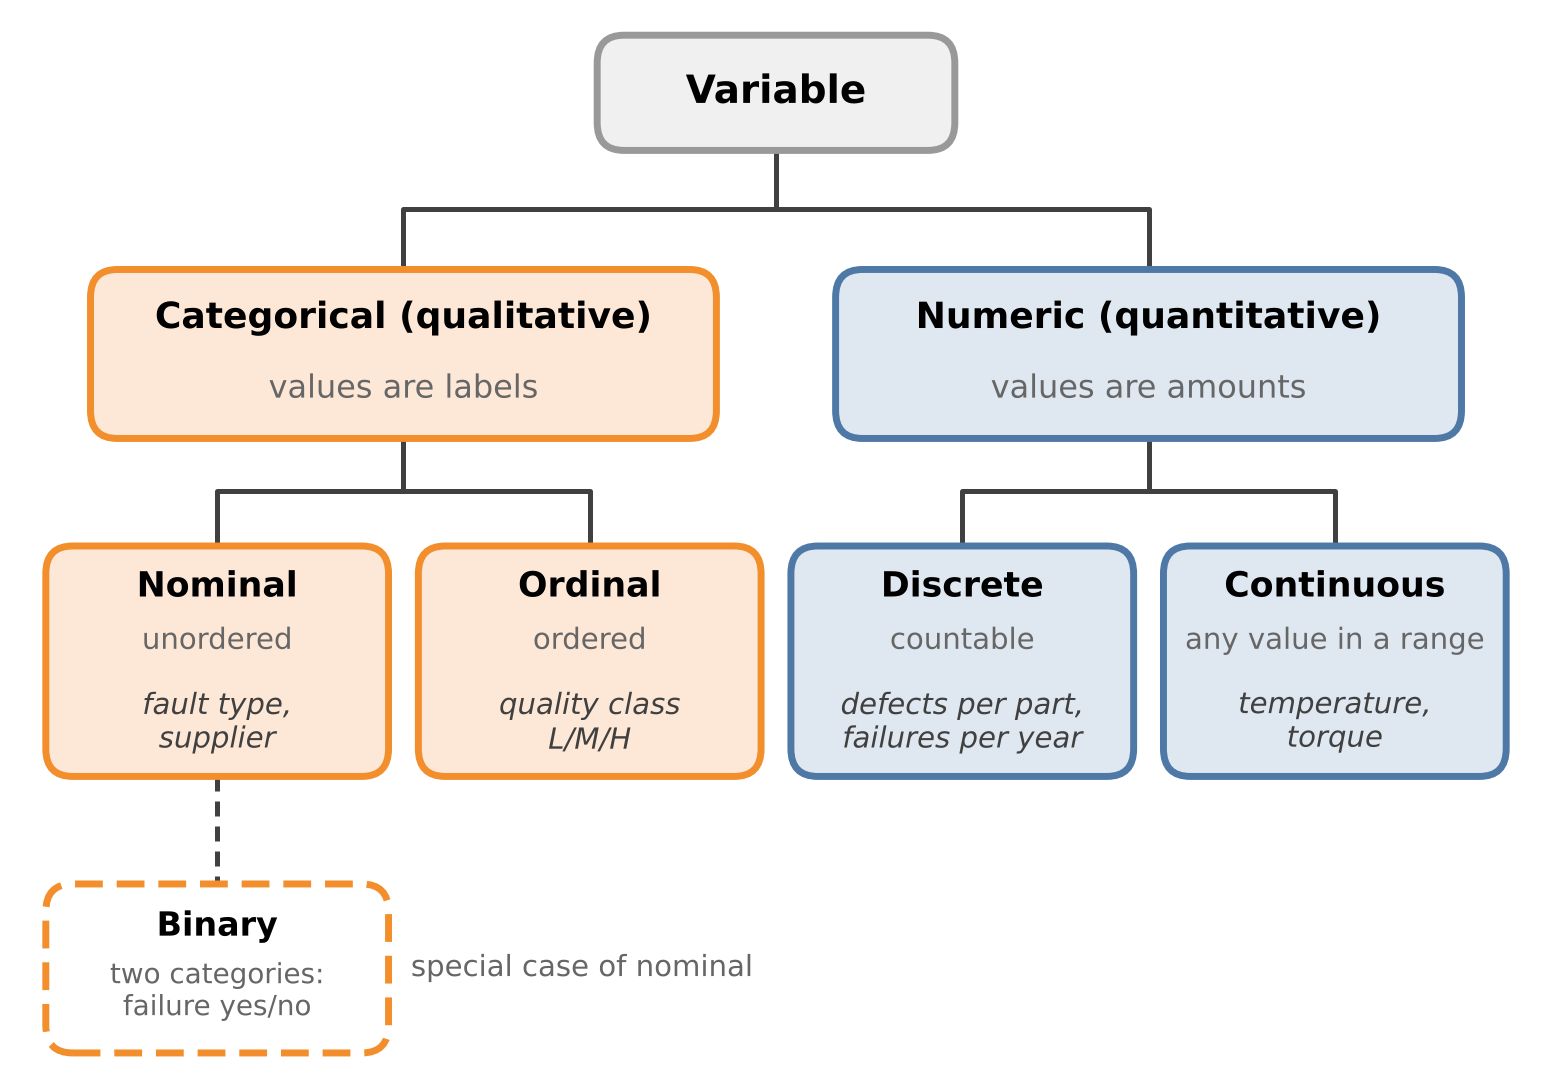
\includegraphics[width=0.75\linewidth,height=\textheight,keepaspectratio]{notebooks/images/variable-types.png}

}

\caption{\label{fig-variable-types}Types of variables with engineering
examples.}

\end{figure}%

For numeric variables we compute means, standard deviations and
histograms; for categorical variables we count frequencies and draw bar
charts. The type also decides which calculations are meaningful at all.
Coding a category as a number does not make it numeric: the mean of the
fault codes 1, 2 and 7 is meaningless. And even for numeric variables,
not every calculation makes sense: 20 °C is 10 K warmer than 10 °C, but
not ``twice as warm'', because the zero of the Celsius scale is
arbitrary -- in kelvin, ratios are meaningful.

In the power plant data, all five variables are continuous, which is
typical for process data. Two kinds of data need special treatment:

\begin{itemize}
\tightlist
\item
  \textbf{Time stamps} are numeric -- the difference between two time
  stamps is a duration -- and mostly serve as the index of a time
  series.
\item
  \textbf{Signals, images and texts} consist of many values per unit,
  e.g.~thousands of samples of a vibration recording. They are condensed
  into a few informative variables, so-called \emph{features} (next
  section) -- either computed by hand, such as the RMS value of a signal
  (Chapter 10), or learned by a neural network (Chapter 12).
\end{itemize}

\subsection{Roles of variables: target and
features}\label{roles-of-variables-target-and-features}

Besides its type, a variable has a role in an analysis. In the power
plant example, we want to predict the electrical output from the ambient
conditions and the condenser pressure:

\begin{itemize}
\tightlist
\item
  The \textbf{target} is the variable we want to explain or predict --
  here the net electrical output (\texttt{PE}). It is also called
  \emph{output}; in classification (Chapter 7), the target is usually
  called \emph{label}.
\item
  The \textbf{features} are the variables used to explain or predict it
  -- here ambient temperature, ambient pressure, relative humidity and
  condenser pressure (\texttt{AT}, \texttt{AP}, \texttt{RH},
  \texttt{V}). They are also called \emph{inputs}.
\end{itemize}

Features can be measured directly or derived from other variables -- the
hour of the day from a time stamp, the RMS value from a vibration
signal. Constructing such features is called \textbf{feature
engineering}; it is where engineering knowledge enters a model most
directly (Chapters 10 and 11).

The role depends on the question, not on the variable: the ambient
temperature is a feature when we predict the power output, but the
target when we forecast the weather. And not every analysis has a target
-- in unsupervised learning (Chapter 9), we look for structure among the
features alone.

\subsection{Something that looks like data -- but is
not}\label{something-that-looks-like-data-but-is-not}

Consider a table with one row per dimension of a turned shaft --
diameter at bearing seat, length, roundness -- and columns \emph{nominal
value}, \emph{upper tolerance}, \emph{lower tolerance}. It has rows,
columns, numbers and units. Is it data?

In the sense of our definition: \textbf{no}. The table comes from the
technical drawing and describes how the shaft \emph{should} be -- a
\textbf{specification}. It contains no observation of any real shaft.
Fitting a model to it would tell us something about the designer's
choices, not about the manufacturing process. The \textbf{data} are the
values the coordinate measuring machine records on the shafts actually
produced. Only by comparing them with the specification can we learn
something about the process -- for example its capability.

Similar cases: a table computed from a formula (a steam table) contains
no information beyond the formula; a production plan is not a record of
production.

\begin{tcolorbox}[enhanced jigsaw, colframe=quarto-callout-tip-color-frame, toprule=.15mm, rightrule=.15mm, title=\textcolor{quarto-callout-tip-color}{\faLightbulb}\hspace{0.5em}{Simulated data}, colbacktitle=quarto-callout-tip-color!10!white, left=2mm, titlerule=0mm, bottomtitle=1mm, toptitle=1mm, opacityback=0, bottomrule=.15mm, breakable, arc=.35mm, opacitybacktitle=0.6, colback=white, coltitle=black, leftrule=.75mm]

Data generated by a simulation are observations of a \textbf{model}, not
of reality. They are extremely useful -- for training, for testing
methods, when real failures are rare -- but every conclusion holds for
the simulated system only, and transfers to reality only as far as the
simulation is valid. Two datasets in this course are simulated: the AI4I
predictive maintenance data and the C-MAPSS turbofan data. We will keep
this in mind when interpreting results.

\end{tcolorbox}

\section{What is data science in
engineering?}\label{what-is-data-science-in-engineering}

Put briefly, data science is the systematic extraction of knowledge and
decisions from data. It combines \emph{statistics} (how to reason under
uncertainty), \emph{computer science} (how to process data and fit
models efficiently) and \emph{domain knowledge} (what the data mean and
which questions matter). How this relates to statistics, machine
learning and AI is sorted out in the next section.

The third ingredient is where engineers have a decisive advantage. A
data scientist without engineering background may find that the
vibration level of a pump correlates with the time of day; an engineer
knows that this is because the pump runs at higher load during the day
shift -- and asks the right follow-up question.

Typical tasks fall into four groups:

\begin{longtable}[]{@{}
  >{\raggedright\arraybackslash}p{(\linewidth - 6\tabcolsep) * \real{0.2500}}
  >{\raggedright\arraybackslash}p{(\linewidth - 6\tabcolsep) * \real{0.2500}}
  >{\raggedright\arraybackslash}p{(\linewidth - 6\tabcolsep) * \real{0.2500}}
  >{\raggedright\arraybackslash}p{(\linewidth - 6\tabcolsep) * \real{0.2500}}@{}}
\toprule\noalign{}
\begin{minipage}[b]{\linewidth}\raggedright
Task
\end{minipage} & \begin{minipage}[b]{\linewidth}\raggedright
Question
\end{minipage} & \begin{minipage}[b]{\linewidth}\raggedright
Engineering example
\end{minipage} & \begin{minipage}[b]{\linewidth}\raggedright
Chapters
\end{minipage} \\
\midrule\noalign{}
\endhead
\bottomrule\noalign{}
\endlastfoot
\textbf{Description} & What happened? & Distribution of tensile strength
in a batch & 2, 3 \\
\textbf{Inference} & Is the effect real? & Did the new supplier change
the scrap rate? & 4, 5 \\
\textbf{Prediction} & What will happen? & Remaining useful life of a
bearing, tomorrow's grid load & 5--8, 11, 12 \\
\textbf{Diagnosis / detection} & What is wrong? & Which fault type? Is
this run abnormal? & 7--10 \\
\end{longtable}

Engineering data have some characteristic properties that we will meet
again and again:

\begin{itemize}
\tightlist
\item
  \textbf{Physics behind the data.} Relationships are often known in
  principle (energy balance, material laws). Good models use this
  knowledge instead of ignoring it.
\item
  \textbf{Rare events.} Failures and defects are -- fortunately -- rare.
  This makes them hard to learn from (Chapter 7).
\item
  \textbf{Time and sequence.} Sensor data are time series. Neighbouring
  values are not independent, which has consequences for validation
  (Chapter 11).
\item
  \textbf{Measurement chains.} Every value went through sensor,
  amplifier, A/D converter, logging system. Each step can introduce
  errors, offsets, gaps and wrong units (Chapter 2).
\item
  \textbf{High cost of errors.} A wrong prediction can mean an unplanned
  standstill or a safety issue. Uncertainty must be quantified and
  communicated.
\end{itemize}

\section{Statistics, machine learning, deep learning, AI: sorting the
terms}\label{statistics-machine-learning-deep-learning-ai-sorting-the-terms}

You have certainly heard all of these terms -- and probably noticed that
they are used inconsistently. Product brochures call a linear regression
``AI'', job advertisements use ``data science'' and ``machine learning''
interchangeably, and research communities draw the borders differently.
There is no official definition. For this course we therefore fix
\textbf{working definitions}: not the only possible ones, but clear
enough to know what we are talking about.

\begin{tcolorbox}[enhanced jigsaw, colframe=quarto-callout-note-color-frame, toprule=.15mm, rightrule=.15mm, title=\textcolor{quarto-callout-note-color}{\faInfo}\hspace{0.5em}{Working definitions used in this course}, colbacktitle=quarto-callout-note-color!10!white, left=2mm, titlerule=0mm, bottomtitle=1mm, toptitle=1mm, opacityback=0, bottomrule=.15mm, breakable, arc=.35mm, opacitybacktitle=0.6, colback=white, coltitle=black, leftrule=.75mm]

\begin{itemize}
\tightlist
\item
  \textbf{Statistics} is the science of learning from data under
  uncertainty: collecting data (sampling, design of experiments),
  describing them, and drawing conclusions with a quantified uncertainty
  (estimates, confidence intervals, tests). Its focus is on
  \emph{understanding} the process that generated the data.
\item
  \textbf{Machine learning (ML)} is the field of algorithms that learn a
  task from examples instead of being explicitly programmed. Its focus
  is on \emph{predicting} well on new, unseen data; models are judged by
  their performance on held-out test data.
\item
  \textbf{Deep learning (DL)} is the part of machine learning that uses
  neural networks with many layers. Such networks learn suitable
  features by themselves, directly from the raw values -- the pixels of
  an image, the samples of a signal, the words of a text -- but
  typically need large amounts of data and computing power.
\item
  \textbf{Artificial intelligence (AI)} is the broadest term: systems
  that perform tasks which would require intelligence if done by humans
  -- perceiving, reasoning, planning, deciding. Machine learning is
  today the dominant approach to AI, but not the only one: rule-based
  expert systems or search and planning algorithms are AI without
  learning.
\item
  \textbf{Data science} is the whole process of turning data into
  knowledge and decisions -- from the question via data acquisition,
  preparation, analysis and modelling to communication and deployment.
  It \emph{uses} statistics and machine learning as tools and requires
  domain knowledge to ask the right questions and interpret the answers.
\end{itemize}

\end{tcolorbox}

\begin{figure}[H]

\centering{

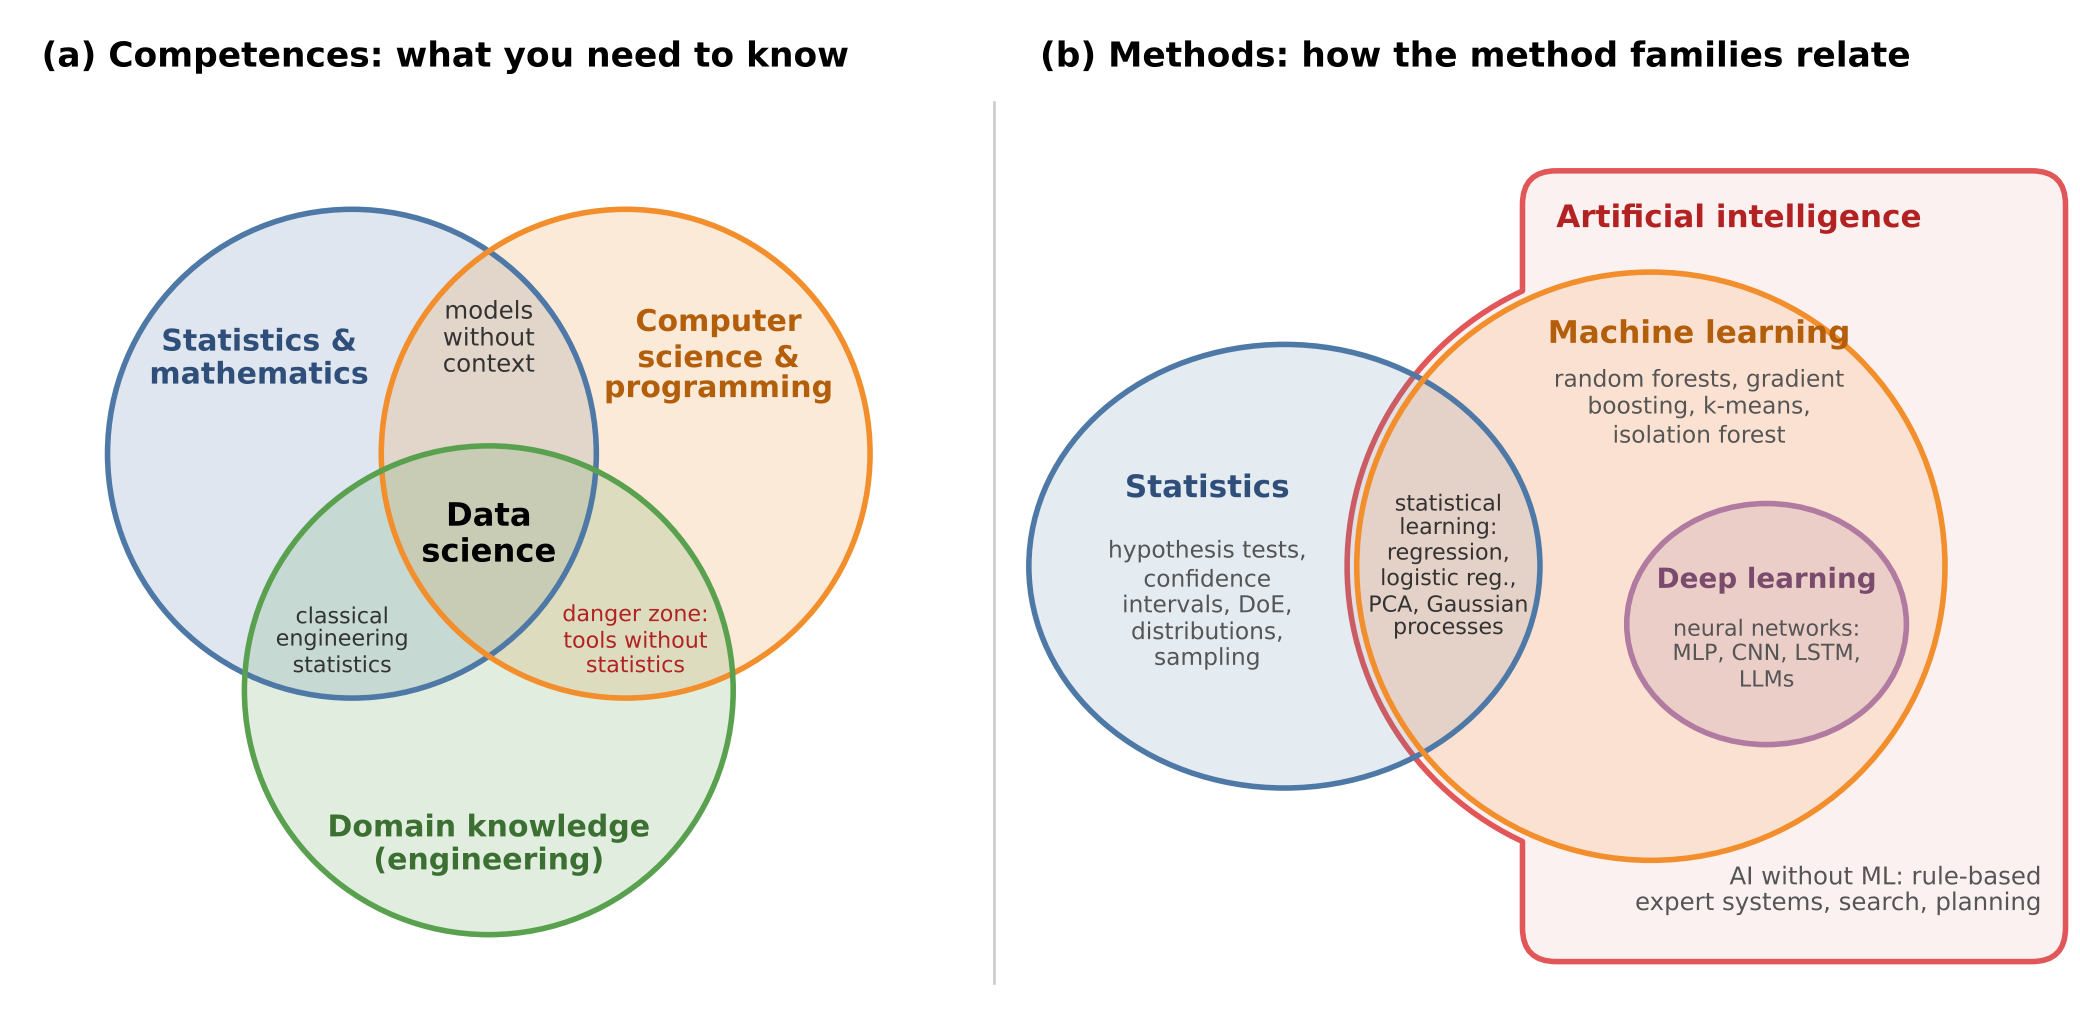
\includegraphics[width=1\linewidth,height=\textheight,keepaspectratio]{notebooks/images/ds-terms.png}

}

\caption{\label{fig-terms}Working definitions used in this course. (a)
Competences: data science lives where statistics, computer science and
domain knowledge meet; any two of them alone fall short. (b) Methods:
deep learning is part of machine learning, which is part of AI;
statistics overlaps strongly with machine learning (``statistical
learning'') but also covers methods outside of it, which are not AI.}

\end{figure}%

The two panels answer different questions. Panel (a) asks what you need
to \emph{know}: data science combines three \textbf{competences}, and
leaving out any one of them leads to typical problems -- models that
answer the wrong engineering question, analyses that do not scale to
large data, or powerful tools used without an understanding of
uncertainty. Panel (b) asks what kind of \emph{method} you use and
arranges the \textbf{method families}.

This is why statistics appears in both panels, with different meanings.
In (a), it is a competence that every data analysis needs -- machine
learning included. In (b), it is a family of methods, of which only one
part, statistical learning, also belongs to machine learning and thus to
AI; a hypothesis test or a confidence interval is statistics, but not
AI. Data science itself does not appear in (b) as a separate region,
because it is defined by its process and purpose, not by a particular
class of methods.

\subsection{Extension: And what about
AI?}\label{extension-and-what-about-ai}

``Artificial intelligence'' is the oldest and the broadest of the terms
-- and today the most overloaded one. The field was founded in the 1950s
with the goal of making machines perform tasks that require
intelligence. For decades, the dominant approach was \textbf{symbolic
AI}: knowledge was written down by experts as rules (``if bearing
temperature \textgreater{} 90 °C and vibration rising, then \ldots{}'')
and combined by logical inference. Such \emph{expert systems} worked in
narrow domains but were laborious to build and brittle when reality
deviated from the rules.

The alternative is to \textbf{learn} the behaviour from data -- machine
learning. Since around 2012, deep neural networks have achieved
breakthroughs in image recognition, speech and text, and today's
\emph{generative AI} (large language models such as the chatbots you
know, image generators) is deep learning trained on enormous amounts of
data. This is why ``AI'' in everyday language now usually means deep
learning -- but the term formally covers much more.

Two distinctions help to keep a clear head:

\begin{itemize}
\tightlist
\item
  \textbf{Narrow vs.~general AI.} All AI systems in practical use,
  including large language models, are built for specific kinds of
  tasks. A system that matches humans across all intellectual tasks
  (\emph{artificial general intelligence}) does not exist and remains a
  matter of research and debate.
\item
  \textbf{Legal vs.~technical meaning.} The EU AI Act defines ``AI
  system'' broadly -- roughly, a machine-based system that infers from
  its input how to produce outputs such as predictions, recommendations
  or decisions -- and attaches obligations depending on the risk of the
  application. For engineers this means that even a fairly simple
  machine learning model in a safety-relevant product can fall under
  regulation.
\end{itemize}

In this course we rarely use the word AI. We say precisely which method
we use -- a test, a regression, a random forest, a neural network --
because that determines its assumptions, its limits and how it must be
validated.

\subsection{Where statistics and machine learning differ -- and where
they
overlap}\label{where-statistics-and-machine-learning-differ-and-where-they-overlap}

The boundary between statistics and machine learning is the most blurred
one, because both fit models to data and many methods belong to both.
The difference lies mainly in the \textbf{goal} and the \textbf{culture}
-- the statistician Leo Breiman famously spoke of ``two cultures'':

\begin{longtable}[]{@{}
  >{\raggedright\arraybackslash}p{(\linewidth - 4\tabcolsep) * \real{0.3333}}
  >{\raggedright\arraybackslash}p{(\linewidth - 4\tabcolsep) * \real{0.3333}}
  >{\raggedright\arraybackslash}p{(\linewidth - 4\tabcolsep) * \real{0.3333}}@{}}
\toprule\noalign{}
\begin{minipage}[b]{\linewidth}\raggedright
\end{minipage} & \begin{minipage}[b]{\linewidth}\raggedright
Statistics
\end{minipage} & \begin{minipage}[b]{\linewidth}\raggedright
Machine learning
\end{minipage} \\
\midrule\noalign{}
\endhead
\bottomrule\noalign{}
\endlastfoot
Main goal & understand and explain: which factors matter, how strong,
how certain? & predict accurately on new data \\
Typical question & ``Does the coolant temperature significantly affect
the tool wear?'' & ``Which tool will fail within the next 100
parts?'' \\
Models & few parameters, interpretable, explicit assumptions & flexible,
often many parameters, ``black box'' accepted \\
Data & often small, carefully designed experiments & often large,
observational (``whatever was logged'') \\
Validation & model assumptions, standard errors, tests & performance on
held-out test data, cross-validation \\
Typical output & estimate ± uncertainty, p-value & prediction, score,
class \\
\end{longtable}

The overlap is large: linear and logistic regression, principal
component analysis and Gaussian processes are standard tools in both
communities -- this common ground is often called \textbf{statistical
learning}. In this course we use both perspectives: when we fit a
regression model in Chapter 5, we look at coefficients and confidence
intervals (statistics) \emph{and} at the prediction error on test data
(machine learning).

\begin{tcolorbox}[enhanced jigsaw, colframe=quarto-callout-important-color-frame, toprule=.15mm, rightrule=.15mm, title=\textcolor{quarto-callout-important-color}{\faExclamation}\hspace{0.5em}{How this course is positioned}, colbacktitle=quarto-callout-important-color!10!white, left=2mm, titlerule=0mm, bottomtitle=1mm, toptitle=1mm, opacityback=0, bottomrule=.15mm, breakable, arc=.35mm, opacitybacktitle=0.6, colback=white, coltitle=black, leftrule=.75mm]

\begin{itemize}
\tightlist
\item
  Chapters 3--5 are mainly \textbf{statistics}: distributions,
  uncertainty, tests, regression, design of experiments.
\item
  Chapters 6--11 are \textbf{statistical learning and machine learning}:
  model selection, classification, ensembles, unsupervised learning,
  signals and time series.
\item
  Chapter 12 gives a first look at \textbf{deep learning}.
\item
  AI methods without learning are not covered. All chapters together
  follow the \textbf{data science} process described next.
\end{itemize}

\end{tcolorbox}

\begin{tcolorbox}[enhanced jigsaw, colframe=quarto-callout-warning-color-frame, toprule=.15mm, rightrule=.15mm, title=\textcolor{quarto-callout-warning-color}{\faExclamationTriangle}\hspace{0.5em}{Pitfall: buzzwords instead of methods}, colbacktitle=quarto-callout-warning-color!10!white, left=2mm, titlerule=0mm, bottomtitle=1mm, toptitle=1mm, opacityback=0, bottomrule=.15mm, breakable, arc=.35mm, opacitybacktitle=0.6, colback=white, coltitle=black, leftrule=.75mm]

When a supplier advertises an ``AI-based'' monitoring system, ask what
is behind it: a threshold rule, a regression model, a random forest or a
neural network? How was it validated, on which data, with which error
rates? The label says nothing about the quality -- the validation does.

\end{tcolorbox}

\section{The CRISP-DM process model}\label{the-crisp-dm-process-model}

Data science projects fail more often for organisational reasons than
for mathematical ones: the wrong question was answered, the data did not
contain the necessary information, or the model was never used. Process
models help to avoid this. The most widely used is CRISP-DM.

\begin{tcolorbox}[enhanced jigsaw, colframe=quarto-callout-note-color-frame, toprule=.15mm, rightrule=.15mm, title=\textcolor{quarto-callout-note-color}{\faInfo}\hspace{0.5em}{Definition: CRISP-DM}, colbacktitle=quarto-callout-note-color!10!white, left=2mm, titlerule=0mm, bottomtitle=1mm, toptitle=1mm, opacityback=0, bottomrule=.15mm, breakable, arc=.35mm, opacitybacktitle=0.6, colback=white, coltitle=black, leftrule=.75mm]

The \emph{Cross-Industry Standard Process for Data Mining} (CRISP-DM)
divides a data science project into six phases: business understanding,
data understanding, data preparation, modelling, evaluation and
deployment. The phases are passed through iteratively, not strictly one
after another.

\end{tcolorbox}

\begin{figure}[H]

\centering{

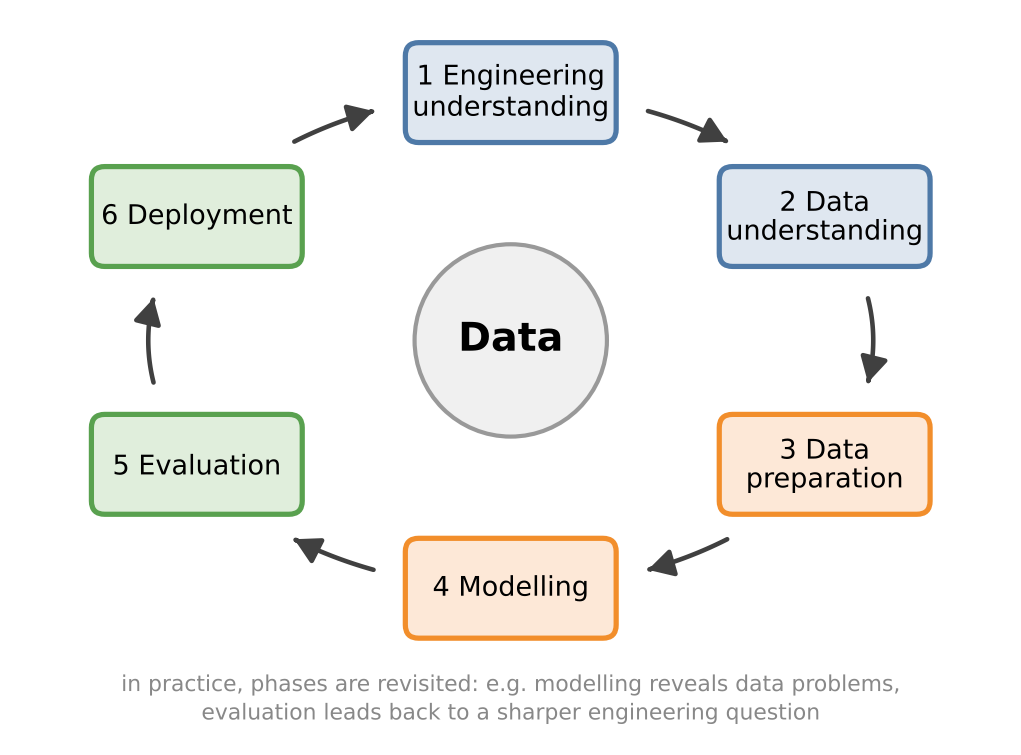
\includegraphics[width=0.65\linewidth,height=\textheight,keepaspectratio]{notebooks/images/crisp-dm.png}

}

\caption{\label{fig-crisp}The CRISP-DM process model. The phases form a
cycle around the data; in practice, the project moves back and forth
between them.}

\end{figure}%

What the phases mean in engineering -- in general and for the day-ahead
commitment of our scenario:

\begin{enumerate}
\def\labelenumi{\arabic{enumi}.}
\tightlist
\item
  \textbf{Engineering understanding} (\emph{business understanding} in
  the original model). Which decision should the analysis support, and
  what does a wrong answer cost? \emph{Power plant:} which output to
  commit for each hour of the next day. Every MWh of deviation costs
  money, so the criterion is economic: switch if the annual savings
  exceed the annual cost of the temperature-based procedure. At noon,
  only a temperature \emph{forecast} for tomorrow is available.
\item
  \textbf{Data understanding.} Which data exist, how were they measured,
  and are the relevant influences measured at all? \emph{Power plant:}
  9,568 hourly averages at full load -- hours below 420 MW were removed
  during cleaning, so a model is only valid for this operating state.
  There are no time stamps, and the temperatures are measured values,
  not forecasts.
\item
  \textbf{Data preparation.} Cleaning, merging data sources, resampling,
  handling missing values, constructing features -- in practice usually
  the largest part of a project. \emph{Power plant:} little to do, the
  table is complete and tidy. In operation, plant records would have to
  be merged with weather forecasts; Chapter 2 shows the pitfalls of raw
  weather files.
\item
  \textbf{Modelling.} Choosing and fitting models -- always together
  with a simple baseline. \emph{Power plant:} the baseline is the flat
  long-term average, the model a straight line for the output as a
  function of the ambient temperature.
\item
  \textbf{Evaluation.} Does the model answer the question, under all
  relevant conditions, and is it better than the baseline? \emph{Power
  plant:} translate the deviations of both rules into annual costs and
  compare them (\emph{Back to the decision}).
\item
  \textbf{Deployment.} Integration into a process, a control system or a
  report -- including monitoring whether the model stays valid.
  \emph{Power plant:} every day before noon, compute the commitment from
  the forecast and record the actual deviations.
\end{enumerate}

\begin{tcolorbox}[enhanced jigsaw, colframe=quarto-callout-tip-color-frame, toprule=.15mm, rightrule=.15mm, title=\textcolor{quarto-callout-tip-color}{\faLightbulb}\hspace{0.5em}{Engineering practice: start with a baseline}, colbacktitle=quarto-callout-tip-color!10!white, left=2mm, titlerule=0mm, bottomtitle=1mm, toptitle=1mm, opacityback=0, bottomrule=.15mm, breakable, arc=.35mm, opacitybacktitle=0.6, colback=white, coltitle=black, leftrule=.75mm]

Before fitting any sophisticated model, compute a trivial baseline: the
mean value, yesterday's value, or a simple physical formula. Every model
must beat the baseline -- otherwise its complexity is not justified.
Surprisingly often, it does not.

\end{tcolorbox}

\begin{tcolorbox}[enhanced jigsaw, colframe=quarto-callout-warning-color-frame, toprule=.15mm, rightrule=.15mm, title=\textcolor{quarto-callout-warning-color}{\faExclamationTriangle}\hspace{0.5em}{Pitfall: answering the wrong question}, colbacktitle=quarto-callout-warning-color!10!white, left=2mm, titlerule=0mm, bottomtitle=1mm, toptitle=1mm, opacityback=0, bottomrule=.15mm, breakable, arc=.35mm, opacitybacktitle=0.6, colback=white, coltitle=black, leftrule=.75mm]

A model that predicts \emph{when} a machine fails is useless if
maintenance can only be scheduled four weeks in advance and the model
warns two days ahead. Clarify the decision and its time horizon in phase
1 -- it determines which data and models make sense.

\end{tcolorbox}

\section{Tools: the Python data
stack}\label{tools-the-python-data-stack}

Python has become the standard language for data science because of its
readable syntax and a large ecosystem of open-source libraries. We use
the following packages:

\begin{longtable}[]{@{}
  >{\raggedright\arraybackslash}p{(\linewidth - 4\tabcolsep) * \real{0.3333}}
  >{\raggedright\arraybackslash}p{(\linewidth - 4\tabcolsep) * \real{0.3333}}
  >{\raggedright\arraybackslash}p{(\linewidth - 4\tabcolsep) * \real{0.3333}}@{}}
\toprule\noalign{}
\begin{minipage}[b]{\linewidth}\raggedright
Package
\end{minipage} & \begin{minipage}[b]{\linewidth}\raggedright
Purpose
\end{minipage} & \begin{minipage}[b]{\linewidth}\raggedright
Typical objects / functions
\end{minipage} \\
\midrule\noalign{}
\endhead
\bottomrule\noalign{}
\endlastfoot
NumPy & n-dimensional arrays, linear algebra, random numbers &
\texttt{np.array}, \texttt{np.mean}, \texttt{np.linalg} \\
pandas & tables and time series, reading and writing files &
\texttt{DataFrame}, \texttt{Series}, \texttt{read\_csv},
\texttt{groupby}, \texttt{resample} \\
Matplotlib & plotting (low level, full control) & \texttt{plt.plot},
\texttt{plt.subplots} \\
seaborn & statistical plots (high level) & \texttt{sns.histplot},
\texttt{sns.pairplot}, \texttt{sns.boxplot} \\
SciPy & statistics, signal processing, optimisation &
\texttt{scipy.stats}, \texttt{scipy.signal}, \texttt{scipy.optimize} \\
statsmodels & statistical models with classical output tables &
\texttt{smf.ols} \\
scikit-learn & machine learning with a uniform interface & \texttt{fit},
\texttt{predict}, \texttt{Pipeline} \\
PyTorch & neural networks (Chapter 12) & \texttt{torch.nn} \\
\end{longtable}

The central data structure is the pandas \textbf{DataFrame}: a table
whose columns have names and data types and whose rows have an index --
for time series typically a time stamp. Most operations are
\emph{vectorised}: instead of looping over rows, we apply an operation
to a whole column at once, which is shorter and much faster.

\begin{tcolorbox}[enhanced jigsaw, colframe=quarto-callout-tip-color-frame, toprule=.15mm, rightrule=.15mm, title=\textcolor{quarto-callout-tip-color}{\faLightbulb}\hspace{0.5em}{Working with notebooks}, colbacktitle=quarto-callout-tip-color!10!white, left=2mm, titlerule=0mm, bottomtitle=1mm, toptitle=1mm, opacityback=0, bottomrule=.15mm, breakable, arc=.35mm, opacitybacktitle=0.6, colback=white, coltitle=black, leftrule=.75mm]

The demo notebooks of the lectures run in
\href{https://colab.research.google.com}{Google Colab} as well as in a
local installation (see the Preface). Packages that are not preinstalled
can be installed from a notebook cell with \texttt{\%pip\ install}. In
Colab, files you download or upload live only as long as the session;
save results you want to keep to Google Drive or download them.

\end{tcolorbox}

\begin{Shaded}
\begin{Highlighting}[]
\CommentTok{\# Setup – every chapter starts with a cell like this one.}

\CommentTok{\# 1) Install packages that are not pre{-}installed in Google Colab or Anaconda.}
\CommentTok{\#    The list depends on the chapter (here it is only one package). The loop}
\CommentTok{\#    checks each package and installs it only if it is missing, so running the}
\CommentTok{\#    cell a second time costs nothing.}
\ImportTok{import}\NormalTok{ importlib.util, subprocess, sys}
\ControlFlowTok{for}\NormalTok{ pkg }\KeywordTok{in}\NormalTok{ [}\StringTok{"ucimlrepo"}\NormalTok{]:}
    \ControlFlowTok{if}\NormalTok{ importlib.util.find\_spec(pkg) }\KeywordTok{is} \VariableTok{None}\NormalTok{:        }\CommentTok{\# package not found?}
\NormalTok{        subprocess.run([sys.executable, }\StringTok{"{-}m"}\NormalTok{, }\StringTok{"pip"}\NormalTok{, }\StringTok{"install"}\NormalTok{, }\StringTok{"{-}q"}\NormalTok{, pkg], check}\OperatorTok{=}\VariableTok{True}\NormalTok{)}

\CommentTok{\# 2) Import the standard data stack (pre{-}installed in Colab and Anaconda).}
\ImportTok{import}\NormalTok{ numpy }\ImportTok{as}\NormalTok{ np}
\ImportTok{import}\NormalTok{ pandas }\ImportTok{as}\NormalTok{ pd}
\ImportTok{import}\NormalTok{ matplotlib.pyplot }\ImportTok{as}\NormalTok{ plt}
\ImportTok{import}\NormalTok{ seaborn }\ImportTok{as}\NormalTok{ sns}

\NormalTok{sns.set\_theme(style}\OperatorTok{=}\StringTok{"whitegrid"}\NormalTok{)                     }\CommentTok{\# common style for all plots}
\end{Highlighting}
\end{Shaded}

\section{Live coding: a first look at the power plant
data}\label{live-coding-a-first-look-at-the-power-plant-data}

A combined cycle power plant (CCPP) combines a gas turbine with a steam
turbine (Figure~\ref{fig-ccpp}). The gas turbine draws in ambient air,
compresses it, burns natural gas in it and drives a generator. Its
exhaust gas is still hot enough to raise steam in a heat recovery steam
generator; the steam drives a second turbine and generator. Behind the
steam turbine, the steam is condensed again in a condenser cooled by
water or air. The plant that supplied our dataset, located in Turkey,
has a nominal capacity of 480 MW: two gas turbines of 160 MW each, two
heat recovery steam generators and one steam turbine of 160 MW
(\href{https://doi.org/10.1016/j.ijepes.2014.02.027}{Tüfekci 2014}).

\begin{figure}[H]

\centering{

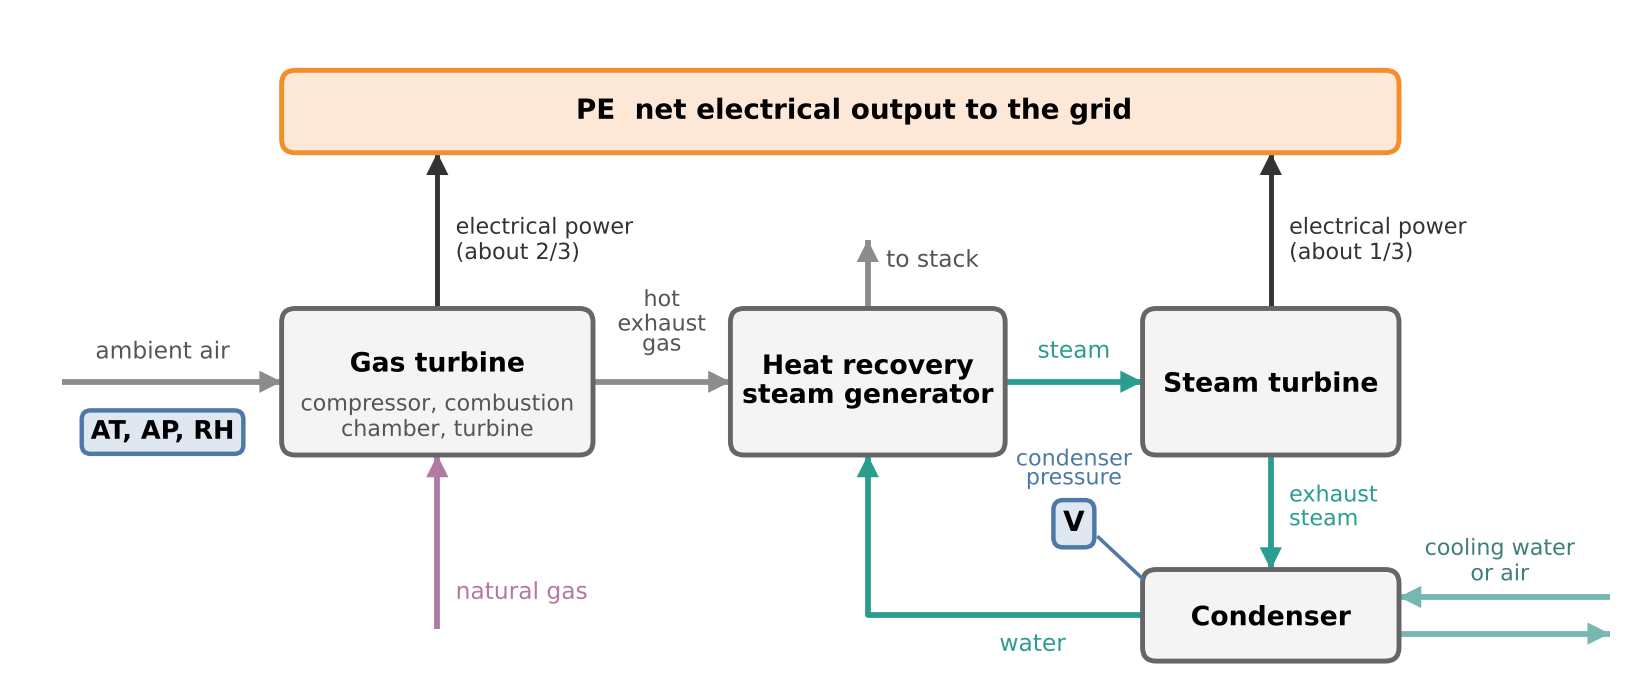
\includegraphics[width=1\linewidth,height=\textheight,keepaspectratio]{notebooks/images/ccpp.png}

}

\caption{\label{fig-ccpp}Simplified block diagram of a combined cycle
power plant with the variables of the dataset. The features (blue)
describe the ambient air and the condenser; the target (orange) is the
net electrical output of gas turbine and steam turbine together.}

\end{figure}%

Why does the weather matter? Warm weather reduces the output twice:

\begin{itemize}
\tightlist
\item
  \textbf{Gas turbine:} warm air is less dense. The compressor draws in
  a smaller mass of air per second, so less fuel can be burnt and the
  gas turbine delivers less power.
\item
  \textbf{Steam turbine:} a turbine delivers the more power, the larger
  the pressure difference between its inlet and its outlet. Cold cooling
  water condenses the steam well and keeps the pressure in the condenser
  low. On warm days, the cooling water is warmer, the condenser pressure
  rises and the steam turbine delivers less power.
\end{itemize}

This is why the condenser pressure is closely linked to the ambient
temperature -- and why we expect the output to fall when either of them
rises.

The dataset contains 9,568 hourly averages from 674 days in six years
(2006--2011), all with the plant at full load. The variables are:

\begin{longtable}[]{@{}
  >{\raggedright\arraybackslash}p{(\linewidth - 6\tabcolsep) * \real{0.2500}}
  >{\raggedright\arraybackslash}p{(\linewidth - 6\tabcolsep) * \real{0.2500}}
  >{\raggedright\arraybackslash}p{(\linewidth - 6\tabcolsep) * \real{0.2500}}
  >{\raggedright\arraybackslash}p{(\linewidth - 6\tabcolsep) * \real{0.2500}}@{}}
\toprule\noalign{}
\begin{minipage}[b]{\linewidth}\raggedright
Column
\end{minipage} & \begin{minipage}[b]{\linewidth}\raggedright
Meaning
\end{minipage} & \begin{minipage}[b]{\linewidth}\raggedright
Unit
\end{minipage} & \begin{minipage}[b]{\linewidth}\raggedright
Role
\end{minipage} \\
\midrule\noalign{}
\endhead
\bottomrule\noalign{}
\endlastfoot
\texttt{AT} & ambient temperature & °C & feature \\
\texttt{V} & exhaust vacuum: pressure in the condenser behind the steam
turbine & cm Hg (according to the documentation -- see below) &
feature \\
\texttt{AP} & ambient pressure & mbar & feature \\
\texttt{RH} & relative humidity & \% & feature \\
\texttt{PE} & net electrical output (hourly average) & MW & target \\
\end{longtable}

The package \texttt{ucimlrepo} downloads datasets from the UCI Machine
Learning Repository directly into pandas.

\begin{Shaded}
\begin{Highlighting}[]
\ImportTok{from}\NormalTok{ ucimlrepo }\ImportTok{import}\NormalTok{ fetch\_ucirepo}

\CommentTok{\# Download dataset no. 294 (Combined Cycle Power Plant) from the UCI repository.}
\CommentTok{\# The number is part of the address of the dataset page:}
\CommentTok{\# archive.ics.uci.edu/dataset/294/combined+cycle+power+plant}
\NormalTok{ccpp }\OperatorTok{=}\NormalTok{ fetch\_ucirepo(}\BuiltInTok{id}\OperatorTok{=}\DecValTok{294}\NormalTok{)}

\CommentTok{\# ucimlrepo returns the features (AT, V, AP, RH) and the target (PE) as two}
\CommentTok{\# separate tables (see "Roles of variables"). pd.concat puts them side by side}
\CommentTok{\# into one DataFrame; axis=1 means "join as columns", not as rows.}
\NormalTok{df }\OperatorTok{=}\NormalTok{ pd.concat([ccpp.data.features, ccpp.data.targets], axis}\OperatorTok{=}\DecValTok{1}\NormalTok{)}

\NormalTok{df.info()   }\CommentTok{\# number of rows, column names, data types, non{-}missing values}
\end{Highlighting}
\end{Shaded}

\begin{verbatim}
<class 'pandas.DataFrame'>
RangeIndex: 9568 entries, 0 to 9567
Data columns (total 5 columns):
 #   Column  Non-Null Count  Dtype  
---  ------  --------------  -----  
 0   AT      9568 non-null   float64
 1   V       9568 non-null   float64
 2   AP      9568 non-null   float64
 3   RH      9568 non-null   float64
 4   PE      9568 non-null   float64
dtypes: float64(5)
memory usage: 373.9 KB
\end{verbatim}

\texttt{df.info()} tells us the number of rows, the column names, the
data types and the number of non-missing values per column. Check the
data types first: pandas stores a column as numbers (\texttt{float64},
\texttt{int64}) only if \emph{every} entry can be read as a number. A
single entry such as \texttt{12,5} (decimal comma) or \texttt{n/a} (a
text marker for a missing value) turns the whole column into text, shown
as \texttt{object}. Calculations then fail or give nonsense -- sorted as
text, \texttt{"10"} comes before \texttt{"9"}. The fix is usually an
argument of \texttt{read\_csv}, e.g.~\texttt{decimal=","} or
\texttt{na\_values={[}"n/a"{]}}. A numeric missing value code such as
\texttt{-999} does not change the type; it shows up only in the summary
statistics (see the weather data in Chapter 2).

Here, all five columns are numeric and complete. The repository also
supplies metadata -- part of the \emph{context} in the sense of our
definition:

\begin{Shaded}
\begin{Highlighting}[]
\NormalTok{ccpp.variables   }\CommentTok{\# metadata supplied by the repository: name, role, type, description, unit}
\end{Highlighting}
\end{Shaded}

\begin{longtable}[]{@{}llllllll@{}}
\toprule\noalign{}
& name & role & type & demographic & description & units &
missing\_values \\
\midrule\noalign{}
\endhead
\bottomrule\noalign{}
\endlastfoot
0 & AT & Feature & Continuous & None & in the range 1.81°C and 37.11°C &
C & no \\
1 & V & Feature & Continuous & None & in teh range 25.36-81.56 cm Hg &
cm Hg & no \\
2 & AP & Feature & Continuous & None & in the range 992.89-1033.30
milibar & milibar & no \\
3 & RH & Feature & Continuous & None & in the range 25.56\% to 100.16\%
& \% & no \\
4 & PE & Target & Continuous & None & 420.26-495.76 MW & MW & no \\
\end{longtable}

Metadata are only as good as the care that went into them -- the unit of
\texttt{V} will show this in a moment.

Next, summary statistics:

\begin{Shaded}
\begin{Highlighting}[]
\NormalTok{df.describe().}\BuiltInTok{round}\NormalTok{(}\DecValTok{2}\NormalTok{)   }\CommentTok{\# one column per variable; round to 2 decimals for readability}
\end{Highlighting}
\end{Shaded}

\begin{longtable}[]{@{}llllll@{}}
\toprule\noalign{}
& AT & V & AP & RH & PE \\
\midrule\noalign{}
\endhead
\bottomrule\noalign{}
\endlastfoot
count & 9568.00 & 9568.00 & 9568.00 & 9568.00 & 9568.00 \\
mean & 19.65 & 54.31 & 1013.26 & 73.31 & 454.37 \\
std & 7.45 & 12.71 & 5.94 & 14.60 & 17.07 \\
min & 1.81 & 25.36 & 992.89 & 25.56 & 420.26 \\
25\% & 13.51 & 41.74 & 1009.10 & 63.33 & 439.75 \\
50\% & 20.34 & 52.08 & 1012.94 & 74.97 & 451.55 \\
75\% & 25.72 & 66.54 & 1017.26 & 84.83 & 468.43 \\
max & 37.11 & 81.56 & 1033.30 & 100.16 & 495.76 \\
\end{longtable}

\begin{tcolorbox}[enhanced jigsaw, colframe=quarto-callout-tip-color-frame, toprule=.15mm, rightrule=.15mm, title=\textcolor{quarto-callout-tip-color}{\faLightbulb}\hspace{0.5em}{How to read \texttt{describe()}}, colbacktitle=quarto-callout-tip-color!10!white, left=2mm, titlerule=0mm, bottomtitle=1mm, toptitle=1mm, opacityback=0, bottomrule=.15mm, breakable, arc=.35mm, opacitybacktitle=0.6, colback=white, coltitle=black, leftrule=.75mm]

Look at each column with an engineer's eye: Are minimum and maximum
physically plausible? Is the mean close to the median (50 \%)? A large
difference indicates a skewed distribution or outliers. Is the standard
deviation large or small compared with the measurement accuracy you
would expect?

\end{tcolorbox}

For the power plant, most ranges are plausible: ambient temperatures
from just above freezing to the mid-thirties, ambient pressures around
1013 mbar, and an output of roughly 420 to 500 MW. The relative humidity
reaches slightly more than 100 \% -- physically impossible, but within
the accuracy of a humidity sensor near saturation. Worth noticing, not
worth correcting.

The lower limit of the output is no coincidence: according to the
original publication, all hours below 420.26 MW were removed as ``out of
range'' during data cleaning. The dataset therefore contains only hours
of high output -- a model fitted to it says nothing about weaker
operating states.

The exhaust vacuum \texttt{V} does not fit, though. According to the
documentation -- and already the original publication -- it is given in
cm Hg, but a vacuum of up to 81.6 cm Hg is impossible: the atmosphere
itself corresponds to only about 76 cm Hg. Moreover, \texttt{V} behaves
like a pressure, not like a vacuum: the larger \texttt{V}, the lower the
output (see the pair plot below). The values would fit the absolute
pressure in the condenser if the unit were mm Hg -- a single wrong
letter -- or mbar. The data alone cannot settle this. For predicting
\texttt{PE}, the unit does not matter; for any physical interpretation,
it does. This is exactly what \emph{numbers without context} means.

A pair plot shows all pairwise relationships at once:

\begin{Shaded}
\begin{Highlighting}[]
\CommentTok{\# Pair plot: a scatter plot for every pair of variables, a histogram of each}
\CommentTok{\# variable on the diagonal.}
\NormalTok{sns.pairplot(}
\NormalTok{    df.sample(}\DecValTok{1000}\NormalTok{, random\_state}\OperatorTok{=}\DecValTok{0}\NormalTok{),   }\CommentTok{\# random subset of 1,000 of the 9,568 rows}
                                       \CommentTok{\# (avoids overplotting); random\_state=0 draws}
                                       \CommentTok{\# the same rows every time the cell is run}
\NormalTok{    corner}\OperatorTok{=}\VariableTok{True}\NormalTok{,                       }\CommentTok{\# lower triangle only – the upper one would}
                                       \CommentTok{\# show the same plots mirrored}
\NormalTok{    plot\_kws}\OperatorTok{=}\NormalTok{\{}\StringTok{"s"}\NormalTok{: }\DecValTok{8}\NormalTok{, }\StringTok{"alpha"}\NormalTok{: }\FloatTok{0.5}\NormalTok{\},   }\CommentTok{\# small (s = marker size), semi{-}transparent}
                                       \CommentTok{\# points (alpha = 0.5), so dense regions}
                                       \CommentTok{\# appear darker}
\NormalTok{)}
\NormalTok{plt.show()}
\end{Highlighting}
\end{Shaded}

\pandocbounded{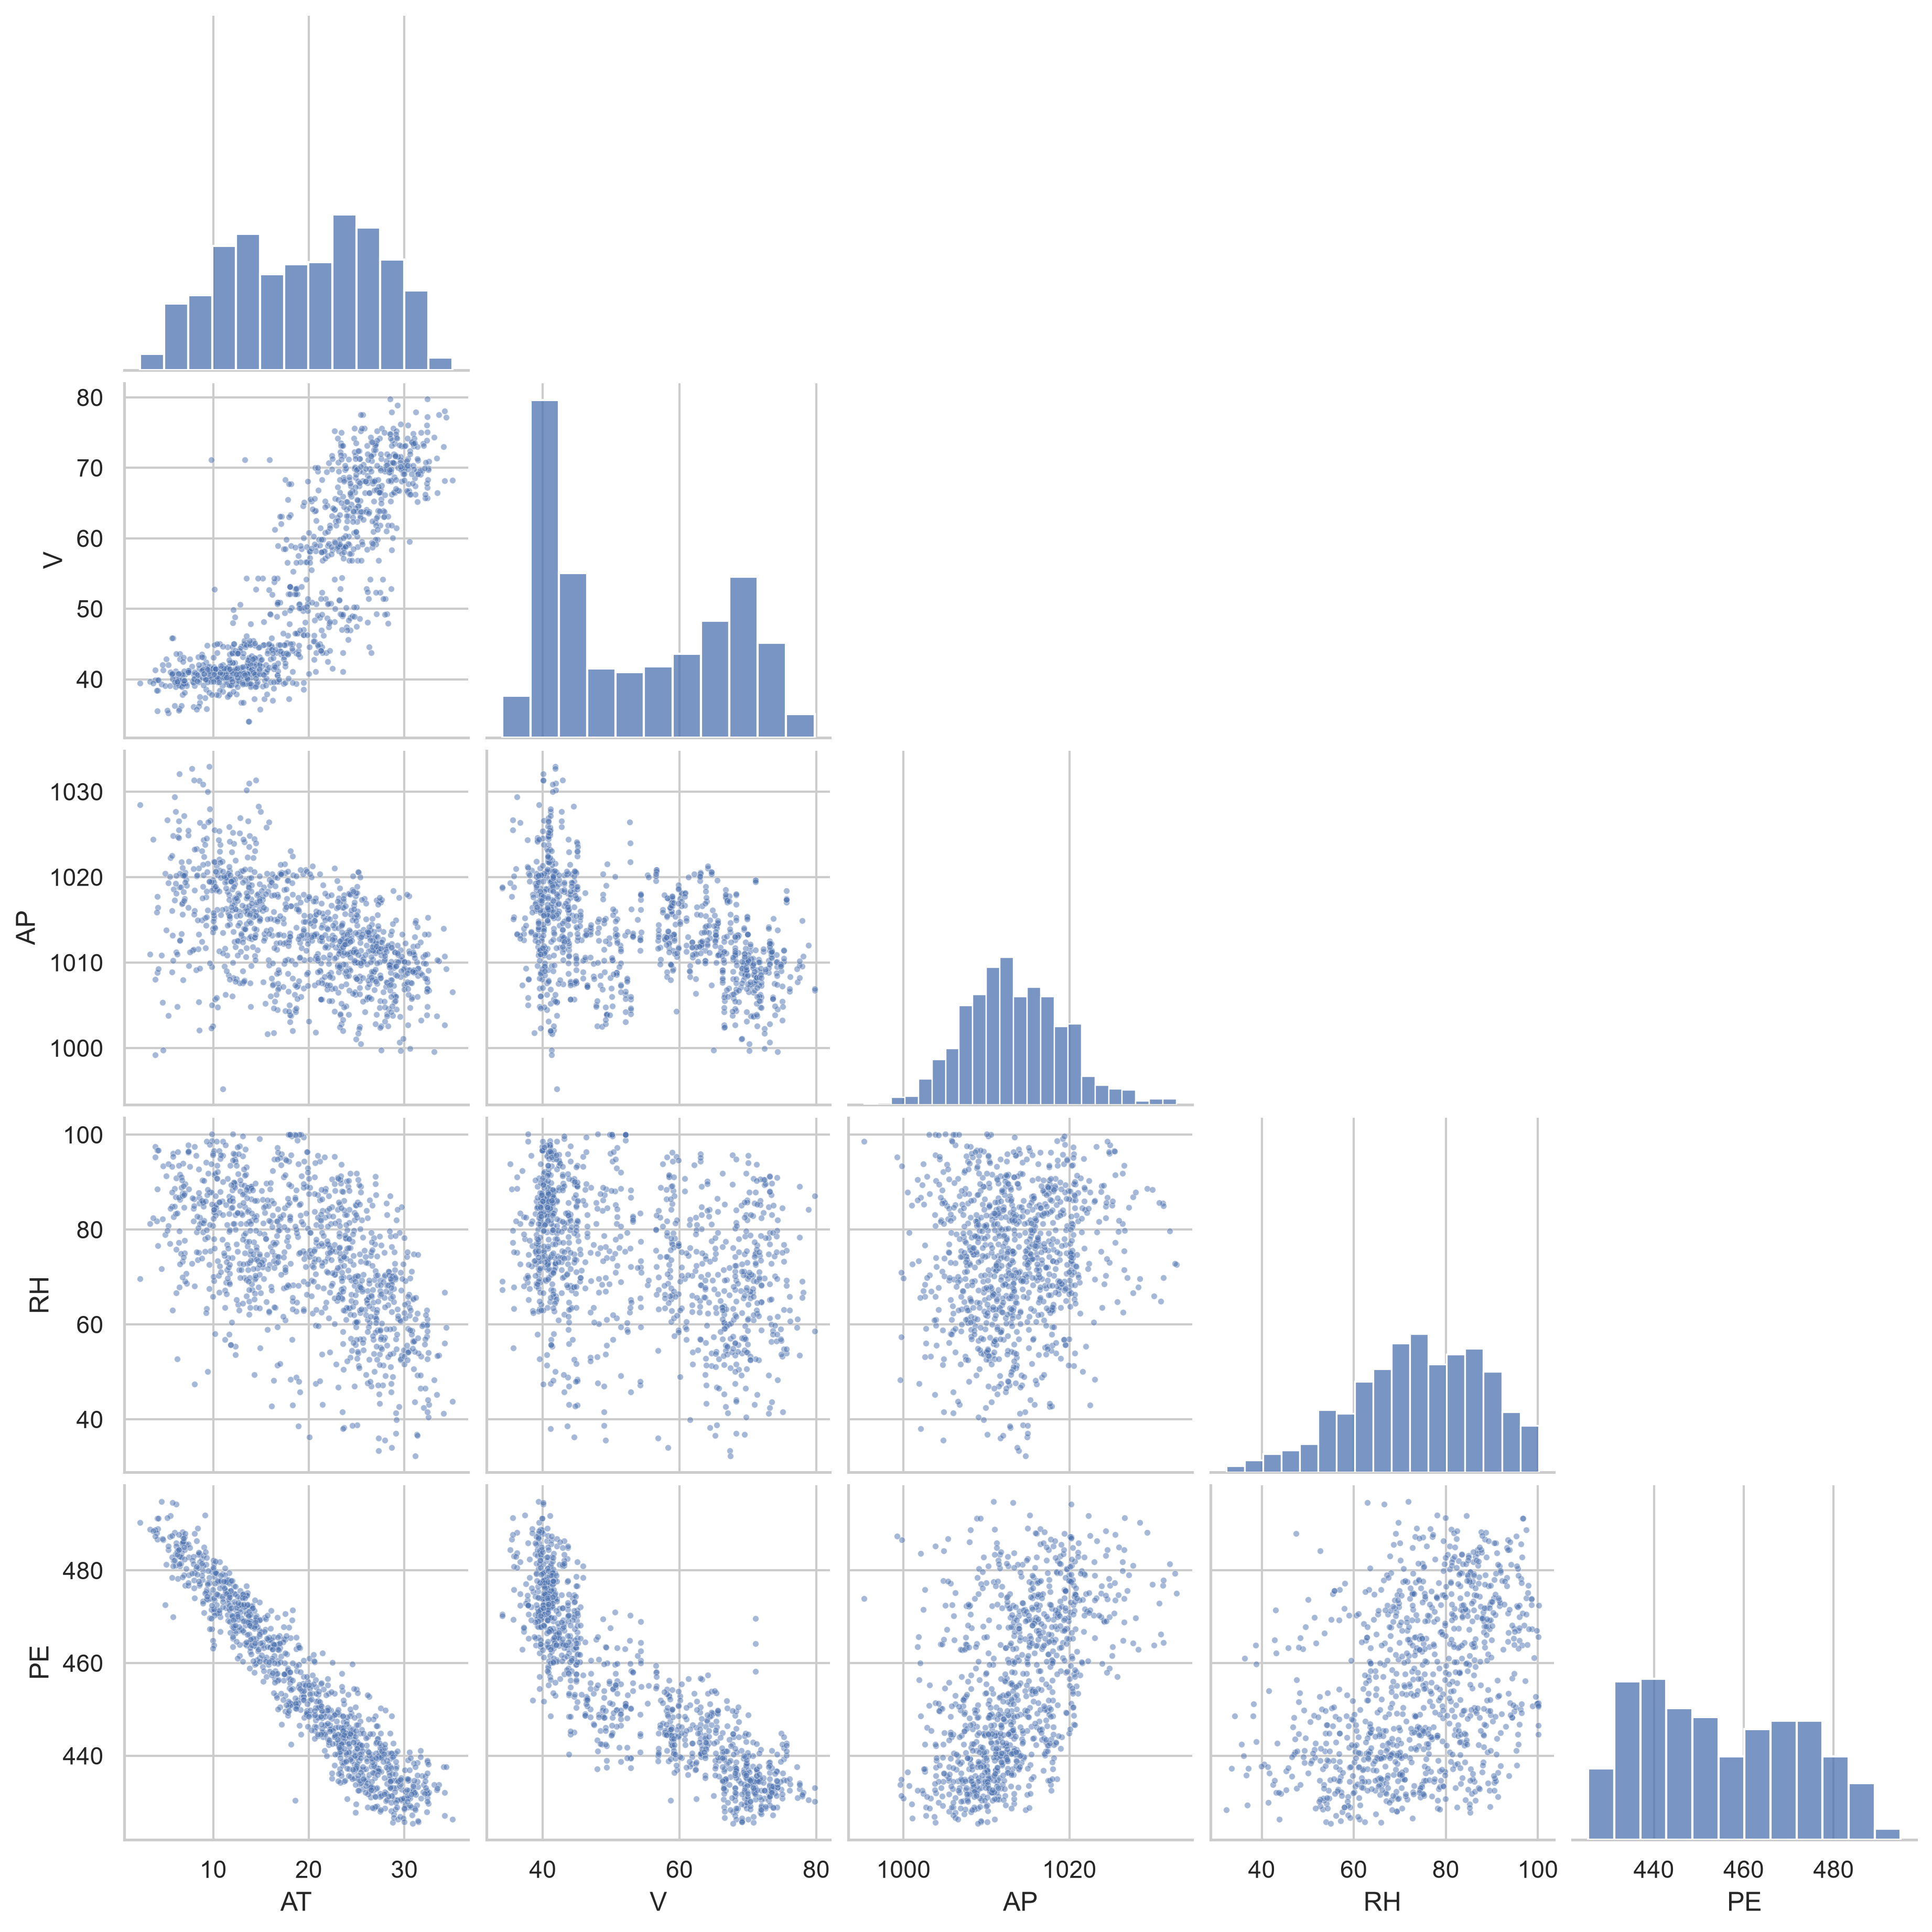
\includegraphics[keepaspectratio]{notebooks/01-workflow_files/figure-pdf/cell-6-output-1.png}}

\textbf{Discussion.} The pair plot is the most informative single figure
for a small tabular dataset. Several observations stand out:

\begin{itemize}
\tightlist
\item
  \texttt{PE} decreases almost linearly with ambient temperature
  \texttt{AT} -- this is the strongest relationship in the data and has
  a clear physical explanation (air density and mass flow).
\item
  \texttt{PE} also decreases with the condenser pressure \texttt{V}, as
  expected from the plant (Figure~\ref{fig-ccpp}).
\item
  \texttt{AT} and \texttt{V} are strongly correlated with each other --
  warm weather means warmer cooling. Such correlated features
  (\emph{collinearity}) make it hard to separate their individual
  effects -- we will return to this in Chapter 5.
\item
  Ambient pressure and humidity show weaker, more diffuse relationships
  with the output.
\end{itemize}

We plotted a random sample of 1,000 points; with all 9,568 points the
scatter plots would be overplotted. Sampling is a simple and legitimate
trick for visual exploration -- but never for computing the final
statistics.

\begin{Shaded}
\begin{Highlighting}[]
\NormalTok{corr }\OperatorTok{=}\NormalTok{ df.corr()                      }\CommentTok{\# Pearson correlation of every pair of columns}
\NormalTok{sns.heatmap(}
\NormalTok{    corr,}
\NormalTok{    annot}\OperatorTok{=}\VariableTok{True}\NormalTok{, fmt}\OperatorTok{=}\StringTok{".2f"}\NormalTok{,            }\CommentTok{\# write each value into its cell, with 2 decimals}
\NormalTok{    cmap}\OperatorTok{=}\StringTok{"RdBu\_r"}\NormalTok{,                    }\CommentTok{\# diverging colour map: red = positive,}
                                      \CommentTok{\# blue = negative (\_r: reversed order of "RdBu")}
\NormalTok{    vmin}\OperatorTok{={-}}\DecValTok{1}\NormalTok{, vmax}\OperatorTok{=}\DecValTok{1}\NormalTok{,                  }\CommentTok{\# colour scale over the full range of r, so that}
                                      \CommentTok{\# white always means r = 0}
\NormalTok{)}
\NormalTok{plt.title(}\StringTok{"Pearson correlation"}\NormalTok{)}
\NormalTok{plt.show()}
\end{Highlighting}
\end{Shaded}

\pandocbounded{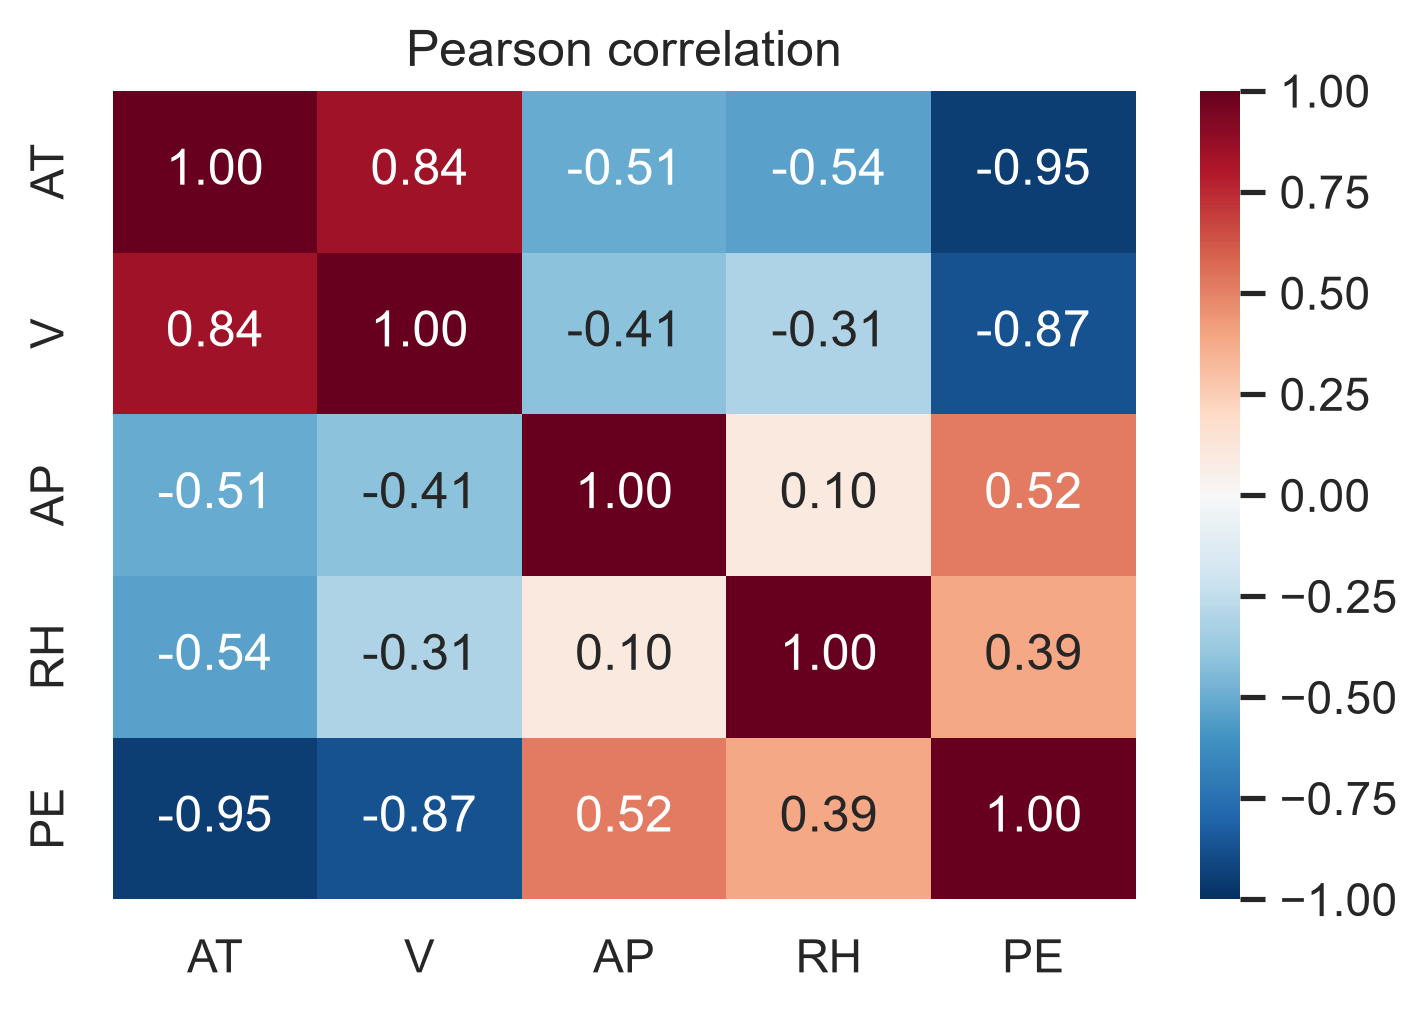
\includegraphics[keepaspectratio]{notebooks/01-workflow_files/figure-pdf/cell-7-output-1.png}}

\begin{tcolorbox}[enhanced jigsaw, colframe=quarto-callout-note-color-frame, toprule=.15mm, rightrule=.15mm, title=\textcolor{quarto-callout-note-color}{\faInfo}\hspace{0.5em}{Definition: Pearson correlation coefficient}, colbacktitle=quarto-callout-note-color!10!white, left=2mm, titlerule=0mm, bottomtitle=1mm, toptitle=1mm, opacityback=0, bottomrule=.15mm, breakable, arc=.35mm, opacitybacktitle=0.6, colback=white, coltitle=black, leftrule=.75mm]

For two variables \(x\) and \(y\) with \(n\) observations,
\[r_{xy} = \frac{\sum_{i=1}^n (x_i - \bar x)(y_i - \bar y)}{\sqrt{\sum_{i=1}^n (x_i - \bar x)^2}\,\sqrt{\sum_{i=1}^n (y_i - \bar y)^2}} \in [-1, 1].\]
It measures the strength of a \textbf{linear} relationship:
\(r = \pm 1\) means all points lie on a straight line, \(r = 0\) means
no linear relationship.

\end{tcolorbox}

\begin{tcolorbox}[enhanced jigsaw, colframe=quarto-callout-warning-color-frame, toprule=.15mm, rightrule=.15mm, title=\textcolor{quarto-callout-warning-color}{\faExclamationTriangle}\hspace{0.5em}{Pitfall: correlation is not causation -- and not every relationship is
linear}, colbacktitle=quarto-callout-warning-color!10!white, left=2mm, titlerule=0mm, bottomtitle=1mm, toptitle=1mm, opacityback=0, bottomrule=.15mm, breakable, arc=.35mm, opacitybacktitle=0.6, colback=white, coltitle=black, leftrule=.75mm]

A correlation near zero does not mean ``no relationship'': \(y = x^2\)
on a symmetric interval has \(r = 0\). And a strong correlation does not
prove a causal effect: both variables may be driven by a third one. In
the power plant, \texttt{V} correlates with \texttt{PE} partly
\emph{because} both depend on the ambient temperature.

\end{tcolorbox}

\subsection{A first simple model}\label{a-first-simple-model}

To make the engineering question concrete, we fit the simplest possible
model: a straight line for \texttt{PE} as a function of \texttt{AT}. We
will treat regression properly in Chapter 5; here we only compare the
line with the trivial baseline that always predicts the mean.

\begin{Shaded}
\begin{Highlighting}[]
\NormalTok{slope, intercept }\OperatorTok{=}\NormalTok{ np.polyfit(df[}\StringTok{"AT"}\NormalTok{], df[}\StringTok{"PE"}\NormalTok{], deg}\OperatorTok{=}\DecValTok{1}\NormalTok{)   }\CommentTok{\# least{-}squares straight line}
                                                             \CommentTok{\# (polynomial of degree 1)}
\NormalTok{pred }\OperatorTok{=}\NormalTok{ intercept }\OperatorTok{+}\NormalTok{ slope }\OperatorTok{*}\NormalTok{ df[}\StringTok{"AT"}\NormalTok{]                          }\CommentTok{\# predicted output for every hour}
\NormalTok{rmse }\OperatorTok{=}\NormalTok{ np.sqrt(np.mean((df[}\StringTok{"PE"}\NormalTok{] }\OperatorTok{{-}}\NormalTok{ pred) }\OperatorTok{**} \DecValTok{2}\NormalTok{))              }\CommentTok{\# root mean squared error}
\BuiltInTok{print}\NormalTok{(}\SpecialStringTok{f"PE ≈ }\SpecialCharTok{\{}\NormalTok{intercept}\SpecialCharTok{:.1f\}}\SpecialStringTok{ MW }\SpecialCharTok{\{}\NormalTok{slope}\SpecialCharTok{:+.2f\}}\SpecialStringTok{ MW/°C · AT,   RMSE = }\SpecialCharTok{\{}\NormalTok{rmse}\SpecialCharTok{:.1f\}}\SpecialStringTok{ MW"}\NormalTok{)}
\CommentTok{\# The RMSE of the constant prediction "mean" is (almost exactly) the standard deviation.}
\BuiltInTok{print}\NormalTok{(}\SpecialStringTok{f"Baseline \textquotesingle{}always predict the mean\textquotesingle{}: RMSE = }\SpecialCharTok{\{}\NormalTok{df[}\StringTok{\textquotesingle{}PE\textquotesingle{}}\NormalTok{]}\SpecialCharTok{.}\NormalTok{std()}\SpecialCharTok{:.1f\}}\SpecialStringTok{ MW"}\NormalTok{)}
\end{Highlighting}
\end{Shaded}

\begin{verbatim}
PE ≈ 497.0 MW -2.17 MW/°C · AT,   RMSE = 5.4 MW
Baseline 'always predict the mean': RMSE = 17.1 MW
\end{verbatim}

The line explains most of the variation: its error (root mean squared
error, RMSE) is a fraction of the error of the trivial mean-value
baseline. Each additional degree Celsius costs about two megawatts of
output. Whether an error of a few MW is ``good enough'' is not a
statistical question -- it depends on the use case defined in CRISP-DM
phase 1.

\section{Back to the decision}\label{back-to-the-decision}

In terms of CRISP-DM, this is phase 5, evaluation: we check the result
against the criterion fixed in phase 1. The trading desk compares two
rules for the committed output: the flat long-term average and the
straight-line estimate from the ambient temperature. To turn the
comparison into an economic decision, we use a deliberately simple cost
model. All figures are assumptions for illustration:

\begin{itemize}
\tightlist
\item
  \textbf{Deviation cost:} every MWh delivered more or less than
  committed costs 30 € extra. (Real imbalance prices vary strongly from
  hour to hour and can be much higher.)
\item
  \textbf{Operating hours:} the plant runs at full load all 8,760 hours
  of a year -- the data contain full-load hours only.
\item
  \textbf{Cost of the new rule:} a weather forecast service,
  implementation and maintenance cost 25,000 € per year.
\end{itemize}

The average deviation in MW -- the \textbf{mean absolute error} (MAE) --
times the number of hours gives the deviation in MWh per year, and times
the price its cost. We switch if the annual savings exceed the annual
cost of the new rule.

\begin{Shaded}
\begin{Highlighting}[]
\CommentTok{\# Simple cost model – all figures are assumptions for illustration}
\NormalTok{price\_dev }\OperatorTok{=} \DecValTok{30}          \CommentTok{\# € per MWh of deviation (extra cost compared with an exact commitment)}
\NormalTok{hours }\OperatorTok{=} \DecValTok{8760}            \CommentTok{\# full{-}load hours per year (simplification: the plant always runs)}
\NormalTok{cost\_rule }\OperatorTok{=} \DecValTok{25\_000}      \CommentTok{\# € per year for the temperature{-}based rule: forecast service,}
                        \CommentTok{\# implementation and maintenance}

\NormalTok{flat\_commitment }\OperatorTok{=}\NormalTok{ df[}\StringTok{"PE"}\NormalTok{].mean()                                     }\CommentTok{\# rule 1: long{-}term average}
\NormalTok{mae\_flat }\OperatorTok{=}\NormalTok{ (df[}\StringTok{"PE"}\NormalTok{] }\OperatorTok{{-}}\NormalTok{ flat\_commitment).}\BuiltInTok{abs}\NormalTok{().mean()                 }\CommentTok{\# mean absolute error (MW)}
\NormalTok{mae\_temp }\OperatorTok{=}\NormalTok{ (df[}\StringTok{"PE"}\NormalTok{] }\OperatorTok{{-}}\NormalTok{ (intercept }\OperatorTok{+}\NormalTok{ slope }\OperatorTok{*}\NormalTok{ df[}\StringTok{"AT"}\NormalTok{])).}\BuiltInTok{abs}\NormalTok{().mean()  }\CommentTok{\# rule 2: straight line}

\CommentTok{\# MW of deviation x hours = MWh of deviation per year; x price = cost per year}
\NormalTok{cost\_flat }\OperatorTok{=}\NormalTok{ mae\_flat }\OperatorTok{*}\NormalTok{ hours }\OperatorTok{*}\NormalTok{ price\_dev}
\NormalTok{cost\_temp }\OperatorTok{=}\NormalTok{ mae\_temp }\OperatorTok{*}\NormalTok{ hours }\OperatorTok{*}\NormalTok{ price\_dev}
\NormalTok{savings }\OperatorTok{=}\NormalTok{ cost\_flat }\OperatorTok{{-}}\NormalTok{ cost\_temp}

\BuiltInTok{print}\NormalTok{(}\SpecialStringTok{f"Average deviation:  flat }\SpecialCharTok{\{}\NormalTok{mae\_flat}\SpecialCharTok{:5.1f\}}\SpecialStringTok{ MW         temperature{-}based }\SpecialCharTok{\{}\NormalTok{mae\_temp}\SpecialCharTok{:5.1f\}}\SpecialStringTok{ MW"}\NormalTok{)}
\BuiltInTok{print}\NormalTok{(}\SpecialStringTok{f"Deviation cost:     flat }\SpecialCharTok{\{}\NormalTok{cost\_flat }\OperatorTok{/} \FloatTok{1e6}\SpecialCharTok{:5.2f\}}\SpecialStringTok{ M€ per year  temperature{-}based }\SpecialCharTok{\{}\NormalTok{cost\_temp }\OperatorTok{/} \FloatTok{1e6}\SpecialCharTok{:5.2f\}}\SpecialStringTok{ M€ per year"}\NormalTok{)}
\BuiltInTok{print}\NormalTok{(}\SpecialStringTok{f"Savings: }\SpecialCharTok{\{}\NormalTok{savings }\OperatorTok{/} \FloatTok{1e6}\SpecialCharTok{:.2f\}}\SpecialStringTok{ M€ per year,  cost of the new rule: }\SpecialCharTok{\{}\NormalTok{cost\_rule }\OperatorTok{/} \FloatTok{1e6}\SpecialCharTok{:.3f\}}\SpecialStringTok{ M€ per year"}\NormalTok{)}
\ControlFlowTok{if}\NormalTok{ savings }\OperatorTok{\textgreater{}}\NormalTok{ cost\_rule:                                               }\CommentTok{\# criterion from phase 1}
    \BuiltInTok{print}\NormalTok{(}\SpecialStringTok{f"Decision: switch to the temperature{-}based estimate "}
          \SpecialStringTok{f"(net benefit }\SpecialCharTok{\{}\NormalTok{(savings }\OperatorTok{{-}}\NormalTok{ cost\_rule) }\OperatorTok{/} \FloatTok{1e6}\SpecialCharTok{:.2f\}}\SpecialStringTok{ M€ per year)."}\NormalTok{)}
\ControlFlowTok{else}\NormalTok{:}
    \BuiltInTok{print}\NormalTok{(}\StringTok{"Decision: keep the flat commitment – the savings do not cover the costs."}\NormalTok{)}

\CommentTok{\# How robust is the decision? Suppose the deviation of rule 2 doubled in operation.}
\NormalTok{savings\_2x }\OperatorTok{=}\NormalTok{ (mae\_flat }\OperatorTok{{-}} \DecValTok{2} \OperatorTok{*}\NormalTok{ mae\_temp) }\OperatorTok{*}\NormalTok{ hours }\OperatorTok{*}\NormalTok{ price\_dev}
\BuiltInTok{print}\NormalTok{(}\SpecialStringTok{f"Robustness: with twice the deviation, the savings would still be }\SpecialCharTok{\{}\NormalTok{savings\_2x }\OperatorTok{/} \FloatTok{1e6}\SpecialCharTok{:.2f\}}\SpecialStringTok{ M€ per year."}\NormalTok{)}
\end{Highlighting}
\end{Shaded}

\begin{verbatim}
Average deviation:  flat  14.8 MW         temperature-based   4.3 MW
Deviation cost:     flat  3.90 M€ per year  temperature-based  1.13 M€ per year
Savings: 2.77 M€ per year,  cost of the new rule: 0.025 M€ per year
Decision: switch to the temperature-based estimate (net benefit 2.75 M€ per year).
Robustness: with twice the deviation, the savings would still be 1.65 M€ per year.
\end{verbatim}

Two caveats belong in the recommendation to the team lead. First, we
evaluated the rule on the same data we used to fit it; Chapter 6 shows
how to evaluate on unseen data. Second, in operation the rule receives a
temperature \emph{forecast}, whose error adds to the error of the model.
Both points make the real benefit smaller. The last line of the output
shows how much room there is: even if the deviation of the
temperature-based rule doubled in operation, the savings would still
exceed the cost of the rule many times over. And the approach is not a
textbook fiction: the plant that supplied the data uses such a model for
its next-day commitment, with the temperature forecast of the national
weather service as input, and reports a mean relative error below 2 \%
in operation
(\href{https://doi.org/10.1016/j.ijepes.2014.02.027}{Tüfekci 2014}).

The cost model is a simplification, too -- Exercise 6 asks you to
question it. Its value lies elsewhere: it turns ``the error is smaller''
into ``the switch is worth this much per year'', which is the language
in which the team lead has to decide.

\begin{tcolorbox}[enhanced jigsaw, colframe=quarto-callout-important-color-frame, toprule=.15mm, rightrule=.15mm, title=\textcolor{quarto-callout-important-color}{\faExclamation}\hspace{0.5em}{Key takeaways}, colbacktitle=quarto-callout-important-color!10!white, left=2mm, titlerule=0mm, bottomtitle=1mm, toptitle=1mm, opacityback=0, bottomrule=.15mm, breakable, arc=.35mm, opacitybacktitle=0.6, colback=white, coltitle=black, leftrule=.75mm]

\begin{itemize}
\tightlist
\item
  Data are recorded values of variables, observed on observational
  units, together with their context. Without unit and meaning, numbers
  cannot be interpreted -- as the condenser pressure \texttt{V} shows.
\item
  Type and role of a variable determine which summaries and models make
  sense.
\item
  Every data science project starts with a precise engineering question
  and a clear criterion for success (CRISP-DM phase 1) -- ideally
  expressed in money, as in the cost model of the power plant.
\item
  Look at the data before modelling: \texttt{info()},
  \texttt{describe()}, pair plots and correlations reveal structure and
  problems quickly.
\item
  Always compare a model with a simple baseline.
\end{itemize}

\end{tcolorbox}

\section{Exercises}\label{exercises}

\begin{enumerate}
\def\labelenumi{\arabic{enumi}.}
\tightlist
\item
  Which columns of the power plant data are features, which is the
  target? Which physical relationships between them do you expect, and
  which signs of the correlations follow from them?
\item
  Fit straight lines for \texttt{PE} against each of the four features
  separately and compare their RMSE. Which single feature is the best
  predictor? Does the ranking agree with the correlation matrix?
\item
  Sketch the six CRISP-DM phases for a project from your own engineering
  background. Which phase do you expect to be the most difficult?
\item
  Place the following in Figure~\ref{fig-terms} (b) and justify: (a) a
  t-test whether a new supplier changes the scrap rate; (b) a
  convolutional neural network that detects cracks in X-ray images; (c)
  route planning for automated guided vehicles with the A* search
  algorithm; (d) a random forest that predicts tool breakage; (e) a
  straight line for power output vs.~temperature with a confidence
  interval for the slope.
\item
  Which of the following are data in the sense of our definition? (a)
  The torque values logged by a screwdriving station for every screw
  joint; (b) the maximum torque in the screwdriver's datasheet; (c) a
  table of thread friction coefficients computed with a formula from a
  handbook; (d) 10,000 lifetimes generated by a reliability simulation;
  (e) a column \texttt{T} with values between 280 and 320, without any
  further information.
\item
  Use the cost model from \emph{Back to the decision}. (a) At which
  deviation price would the savings just cover the cost of the new rule
  (break-even)? (b) How large may the average deviation of the
  temperature-based rule become in operation before switching no longer
  pays off? (c) Which simplifications of the cost model would you
  question first, and in which direction would they change the result?
\end{enumerate}

\subsection{Solutions}\label{solutions}

\begin{tcolorbox}[enhanced jigsaw, colframe=quarto-callout-caution-color-frame, toprule=.15mm, rightrule=.15mm, title=\textcolor{quarto-callout-caution-color}{\faFire}\hspace{0.5em}{Solution to Exercise 1}, colbacktitle=quarto-callout-caution-color!10!white, left=2mm, titlerule=0mm, bottomtitle=1mm, toptitle=1mm, opacityback=0, bottomrule=.15mm, breakable, arc=.35mm, opacitybacktitle=0.6, colback=white, coltitle=black, leftrule=.75mm]

The features are the ambient conditions \texttt{AT}, \texttt{AP},
\texttt{RH} and the condenser pressure \texttt{V}; the target is
\texttt{PE}. Strictly speaking, \texttt{V} is not an ambient condition
but a plant variable -- it depends on the cooling water temperature and
therefore also on the weather (Figure~\ref{fig-ccpp}).

Expected signs: higher ambient temperature lowers air density and thus
the mass flow and power of the gas turbine → negative correlation of
\texttt{AT} with \texttt{PE}. A higher condenser pressure (worse vacuum,
larger \texttt{V} in this dataset) reduces the pressure difference
across the steam turbine → negative correlation of \texttt{V} with
\texttt{PE}. Higher ambient pressure increases air density → positive
correlation. Humidity has a smaller, less obvious effect. The
correlation matrix confirms these signs.

\end{tcolorbox}

\begin{tcolorbox}[enhanced jigsaw, colframe=quarto-callout-caution-color-frame, toprule=.15mm, rightrule=.15mm, title=\textcolor{quarto-callout-caution-color}{\faFire}\hspace{0.5em}{Solution to Exercise 2}, colbacktitle=quarto-callout-caution-color!10!white, left=2mm, titlerule=0mm, bottomtitle=1mm, toptitle=1mm, opacityback=0, bottomrule=.15mm, breakable, arc=.35mm, opacitybacktitle=0.6, colback=white, coltitle=black, leftrule=.75mm]

\begin{Shaded}
\begin{Highlighting}[]
\NormalTok{rows }\OperatorTok{=}\NormalTok{ []}
\ControlFlowTok{for}\NormalTok{ col }\KeywordTok{in}\NormalTok{ [}\StringTok{"AT"}\NormalTok{, }\StringTok{"V"}\NormalTok{, }\StringTok{"AP"}\NormalTok{, }\StringTok{"RH"}\NormalTok{]:                       }\CommentTok{\# one straight line per feature}
\NormalTok{    b1, b0 }\OperatorTok{=}\NormalTok{ np.polyfit(df[col], df[}\StringTok{"PE"}\NormalTok{], deg}\OperatorTok{=}\DecValTok{1}\NormalTok{)         }\CommentTok{\# slope b1, intercept b0}
\NormalTok{    rmse\_col }\OperatorTok{=}\NormalTok{ np.sqrt(np.mean((df[}\StringTok{"PE"}\NormalTok{] }\OperatorTok{{-}}\NormalTok{ (b0 }\OperatorTok{+}\NormalTok{ b1 }\OperatorTok{*}\NormalTok{ df[col])) }\OperatorTok{**} \DecValTok{2}\NormalTok{))}
\NormalTok{    rows.append(\{}\StringTok{"feature"}\NormalTok{: col, }\StringTok{"slope"}\NormalTok{: b1, }\StringTok{"RMSE (MW)"}\NormalTok{: rmse\_col, }\StringTok{"r"}\NormalTok{: df[col].corr(df[}\StringTok{"PE"}\NormalTok{])\})}
\NormalTok{pd.DataFrame(rows).sort\_values(}\StringTok{"RMSE (MW)"}\NormalTok{).}\BuiltInTok{round}\NormalTok{(}\DecValTok{3}\NormalTok{)      }\CommentTok{\# best feature first}
\end{Highlighting}
\end{Shaded}

\begin{longtable}[]{@{}lllll@{}}
\toprule\noalign{}
& feature & slope & RMSE (MW) & r \\
\midrule\noalign{}
\endhead
\bottomrule\noalign{}
\endlastfoot
0 & AT & -2.171 & 5.425 & -0.948 \\
1 & V & -1.168 & 8.421 & -0.870 \\
2 & AP & 1.490 & 14.594 & 0.518 \\
3 & RH & 0.456 & 15.716 & 0.390 \\
\end{longtable}

\texttt{AT} gives by far the smallest RMSE, followed by \texttt{V}. For
a straight-line fit, the ranking by RMSE is exactly the ranking by
\(|r|\), because the fraction of explained variance of a simple linear
regression is \(r^2\). The original publication reports practically the
same values (\href{https://doi.org/10.1016/j.ijepes.2014.02.027}{Tüfekci
2014}).

\end{tcolorbox}

\begin{tcolorbox}[enhanced jigsaw, colframe=quarto-callout-caution-color-frame, toprule=.15mm, rightrule=.15mm, title=\textcolor{quarto-callout-caution-color}{\faFire}\hspace{0.5em}{Solution to Exercise 3}, colbacktitle=quarto-callout-caution-color!10!white, left=2mm, titlerule=0mm, bottomtitle=1mm, toptitle=1mm, opacityback=0, bottomrule=.15mm, breakable, arc=.35mm, opacitybacktitle=0.6, colback=white, coltitle=black, leftrule=.75mm]

There is no single correct answer. A good sketch states a concrete
decision in phase 1 (e.g.~``decide weekly which tools to replace''),
names the data sources and their owners in phase 2, lists expected
preparation steps in phase 3 (merging, time alignment), names a baseline
in phase 4, an evaluation criterion tied to the decision in phase 5
(e.g.~cost of unplanned stops), and a realistic deployment path in phase
6. Many practitioners name phase 2/3 (data access and quality) or phase
6 (deployment and acceptance) as the hardest.

\end{tcolorbox}

\begin{tcolorbox}[enhanced jigsaw, colframe=quarto-callout-caution-color-frame, toprule=.15mm, rightrule=.15mm, title=\textcolor{quarto-callout-caution-color}{\faFire}\hspace{0.5em}{Solution to Exercise 4}, colbacktitle=quarto-callout-caution-color!10!white, left=2mm, titlerule=0mm, bottomtitle=1mm, toptitle=1mm, opacityback=0, bottomrule=.15mm, breakable, arc=.35mm, opacitybacktitle=0.6, colback=white, coltitle=black, leftrule=.75mm]

\begin{enumerate}
\def\labelenumi{(\alph{enumi})}
\tightlist
\item
  \textbf{Statistics} -- inference about a difference with quantified
  uncertainty, no prediction task. (b) \textbf{Deep learning} (and thus
  ML and AI) -- a neural network learns features from raw images. (c)
  \textbf{AI without machine learning} -- A* is a search algorithm;
  nothing is learned from data. (d) \textbf{Machine learning} -- a
  flexible model optimised for predictive accuracy; it is not deep
  learning. (e) The \textbf{overlap of statistics and machine learning}:
  the same linear model, used here in the statistical way
  (interpretation of the slope and its uncertainty). Used purely to
  predict output for the day-ahead market and validated on test data, it
  would be viewed as machine learning. The examples show that the method
  alone does not determine the category -- the purpose matters too.
\end{enumerate}

\end{tcolorbox}

\begin{tcolorbox}[enhanced jigsaw, colframe=quarto-callout-caution-color-frame, toprule=.15mm, rightrule=.15mm, title=\textcolor{quarto-callout-caution-color}{\faFire}\hspace{0.5em}{Solution to Exercise 5}, colbacktitle=quarto-callout-caution-color!10!white, left=2mm, titlerule=0mm, bottomtitle=1mm, toptitle=1mm, opacityback=0, bottomrule=.15mm, breakable, arc=.35mm, opacitybacktitle=0.6, colback=white, coltitle=black, leftrule=.75mm]

\begin{enumerate}
\def\labelenumi{(\alph{enumi})}
\tightlist
\item
  \textbf{Data} -- recorded observations of real screw joints (provided
  we know the unit and which joint each value belongs to). (b)
  \textbf{Not data} -- a specification of what the tool is designed for,
  not an observation. (c) \textbf{Not data} about any real joint -- the
  table only re-expresses the formula; a model fitted to it would
  rediscover the formula. (d) \textbf{Data about a model} -- valid
  observations of the simulation; conclusions hold for real products
  only as far as the simulation is valid. (e) \textbf{Not usable as
  data} -- the numbers might be temperatures in kelvin, but without
  unit, sensor and time stamp they cannot be interpreted. They become
  data once the context is recovered.
\end{enumerate}

\end{tcolorbox}

\begin{tcolorbox}[enhanced jigsaw, colframe=quarto-callout-caution-color-frame, toprule=.15mm, rightrule=.15mm, title=\textcolor{quarto-callout-caution-color}{\faFire}\hspace{0.5em}{Solution to Exercise 6}, colbacktitle=quarto-callout-caution-color!10!white, left=2mm, titlerule=0mm, bottomtitle=1mm, toptitle=1mm, opacityback=0, bottomrule=.15mm, breakable, arc=.35mm, opacitybacktitle=0.6, colback=white, coltitle=black, leftrule=.75mm]

\begin{Shaded}
\begin{Highlighting}[]
\CommentTok{\# (a) price at which the savings equal the cost of the rule}
\NormalTok{price\_break }\OperatorTok{=}\NormalTok{ cost\_rule }\OperatorTok{/}\NormalTok{ ((mae\_flat }\OperatorTok{{-}}\NormalTok{ mae\_temp) }\OperatorTok{*}\NormalTok{ hours)}
\CommentTok{\# (b) deviation of rule 2 at which the savings equal the cost of the rule}
\NormalTok{mae\_break }\OperatorTok{=}\NormalTok{ mae\_flat }\OperatorTok{{-}}\NormalTok{ cost\_rule }\OperatorTok{/}\NormalTok{ (hours }\OperatorTok{*}\NormalTok{ price\_dev)}
\BuiltInTok{print}\NormalTok{(}\SpecialStringTok{f"(a) break{-}even price:     }\SpecialCharTok{\{}\NormalTok{price\_break}\SpecialCharTok{:.2f\}}\SpecialStringTok{ € per MWh (assumed: }\SpecialCharTok{\{}\NormalTok{price\_dev}\SpecialCharTok{\}}\SpecialStringTok{ € per MWh)"}\NormalTok{)}
\BuiltInTok{print}\NormalTok{(}\SpecialStringTok{f"(b) break{-}even deviation: }\SpecialCharTok{\{}\NormalTok{mae\_break}\SpecialCharTok{:.1f\}}\SpecialStringTok{ MW (today: }\SpecialCharTok{\{}\NormalTok{mae\_temp}\SpecialCharTok{:.1f\}}\SpecialStringTok{ MW, flat rule: }\SpecialCharTok{\{}\NormalTok{mae\_flat}\SpecialCharTok{:.1f\}}\SpecialStringTok{ MW)"}\NormalTok{)}
\end{Highlighting}
\end{Shaded}

\begin{verbatim}
(a) break-even price:     0.27 € per MWh (assumed: 30 € per MWh)
(b) break-even deviation: 14.7 MW (today: 4.3 MW, flat rule: 14.8 MW)
\end{verbatim}

\begin{enumerate}
\def\labelenumi{(\alph{enumi})}
\item
  Even a deviation price far below 1 € per MWh would cover the cost of
  the rule -- real prices are much higher. (b) The rule pays off as long
  as it is even slightly better than the flat commitment: the break-even
  deviation lies only about 0.1 MW below that of the flat rule. With
  well over 100,000 MWh of deviation per year, even small improvements
  are worth a lot of money.
\item
  For example: deviations in the two directions are usually priced
  differently, and the price depends on the state of the grid; the plant
  does not run at full load in every hour (maintenance, partial load),
  so fewer hours mean smaller savings; the forecast error of the
  temperature increases the deviation of the new rule; and the cost of
  the new rule may be underestimated (staff time, IT). None of these is
  likely to reverse the decision here -- but in a project with a smaller
  margin, each of them could.
\end{enumerate}

\end{tcolorbox}

\chapter{Exploratory Data Analysis and Data
Quality}\label{exploratory-data-analysis-and-data-quality}

Exploratory data analysis (EDA) is the systematic first look at a
dataset before any model is built. Its purpose is twofold: to understand
the structure of the data -- distributions, relationships, patterns over
time -- and to find problems -- gaps, outliers, implausible values,
inconsistencies. In engineering, a large share of failed data science
projects can be traced back to data problems that a careful EDA would
have revealed.

The statistician John Tukey, who coined the term, put it this way: EDA
is detective work. We look for clues without knowing in advance what we
will find. The tools are simple -- summary statistics and plots -- but
using them well requires domain knowledge.

\textbf{Scenario: go or no-go for a failure prediction project}

A semiconductor fab wants to predict failed production runs from its
process data. A project budget for one year has been requested, and the
fab manager asks you for a quick assessment before signing: ``We have
almost 600 sensors and more than 1,500 runs -- that must be enough,
right?'' You have one week to look at the data.

\textbf{Your decision:} Recommend starting the project now, or first
investing in better data?

\textbf{Learning goals.} After this chapter you can

\begin{itemize}
\tightlist
\item
  describe distributions numerically (location, spread, shape) and
  visually (histogram, box plot),
\item
  explore a multivariate sensor dataset with time series plots, profiles
  and heatmaps,
\item
  detect outliers with the IQR rule and robust z-scores and decide how
  to treat them,
\item
  characterise missing data (MCAR, MAR, MNAR) and choose an appropriate
  treatment,
\item
  read a raw sensor file correctly (separator, missing value code, time
  stamps, time zone),
\item
  resample and aggregate time series correctly,
\item
  judge whether a dataset is fit for the intended analysis.
\end{itemize}

\textbf{Datasets in this chapter}

\begin{itemize}
\tightlist
\item
  \href{https://archive.ics.uci.edu/dataset/374/appliances+energy+prediction}{Appliances
  Energy Prediction (UCI)}
\item
  \href{https://archive.ics.uci.edu/dataset/179/secom}{SECOM (UCI)}
\item
  \href{https://opendata.dwd.de/climate_environment/CDC/}{DWD Climate
  Data Center -- hourly station data}
\end{itemize}

\section{Describing distributions}\label{describing-distributions}

A single variable is described by its \textbf{location} (where are the
values?), its \textbf{spread} (how much do they vary?) and its
\textbf{shape} (symmetric, skewed, multimodal?).

\begin{tcolorbox}[enhanced jigsaw, colframe=quarto-callout-note-color-frame, toprule=.15mm, rightrule=.15mm, title=\textcolor{quarto-callout-note-color}{\faInfo}\hspace{0.5em}{Definition: Location and spread}, colbacktitle=quarto-callout-note-color!10!white, left=2mm, titlerule=0mm, bottomtitle=1mm, toptitle=1mm, opacityback=0, bottomrule=.15mm, breakable, arc=.35mm, opacitybacktitle=0.6, colback=white, coltitle=black, leftrule=.75mm]

For observations \(x_1, \dots, x_n\):

\begin{itemize}
\tightlist
\item
  \textbf{Mean} \(\bar x = \frac{1}{n}\sum_i x_i\) and \textbf{median}
  (the middle value of the sorted data).
\item
  \textbf{Sample standard deviation}
  \(s = \sqrt{\frac{1}{n-1}\sum_i (x_i - \bar x)^2}\).
\item
  \textbf{Quartiles} \(Q_1\), \(Q_3\) (25 \% and 75 \% quantiles) and
  the \textbf{interquartile range} \(\text{IQR} = Q_3 - Q_1\).
\item
  \textbf{Median absolute deviation:} with the median
  \(\tilde x = \operatorname{median}(x_1, \dots, x_n)\),
  \[\text{MAD} = \operatorname{median}\big(|x_1 - \tilde x|, \dots, |x_n - \tilde x|\big),\]
  i.e.~the median of the absolute deviations from the median.
\end{itemize}

\end{tcolorbox}

Mean and standard deviation are sensitive to extreme values: a single
wrong reading of \(10^6\) can dominate both. Median, IQR and MAD are
\textbf{robust}: they barely change if a few values are wrong. For
engineering data, where sensor glitches are common, it pays to look at
both and compare them.

\begin{tcolorbox}[enhanced jigsaw, colframe=quarto-callout-tip-color-frame, toprule=.15mm, rightrule=.15mm, title=\textcolor{quarto-callout-tip-color}{\faLightbulb}\hspace{0.5em}{Which plot for which question?}, colbacktitle=quarto-callout-tip-color!10!white, left=2mm, titlerule=0mm, bottomtitle=1mm, toptitle=1mm, opacityback=0, bottomrule=.15mm, breakable, arc=.35mm, opacitybacktitle=0.6, colback=white, coltitle=black, leftrule=.75mm]

\begin{itemize}
\tightlist
\item
  \emph{Distribution of one variable:} histogram (shape) or box plot
  (compact, good for comparing groups).
\item
  \emph{Relationship between two variables:} scatter plot; with many
  points use transparency or hexbin plots.
\item
  \emph{Development over time:} line plot, possibly with a rolling mean.
\item
  \emph{Patterns over two time scales} (hour of day × weekday): heatmap.
\item
  \emph{Many variables at once:} correlation heatmap, pair plot of a
  subset.
\end{itemize}

\end{tcolorbox}

\section{Data quality in engineering
data}\label{data-quality-in-engineering-data}

Measured data pass through a long chain -- sensor, signal conditioning,
A/D conversion, data logger, database, export -- and every link can
introduce errors. Typical problems:

\begin{longtable}[]{@{}
  >{\raggedright\arraybackslash}p{(\linewidth - 4\tabcolsep) * \real{0.3333}}
  >{\raggedright\arraybackslash}p{(\linewidth - 4\tabcolsep) * \real{0.3333}}
  >{\raggedright\arraybackslash}p{(\linewidth - 4\tabcolsep) * \real{0.3333}}@{}}
\toprule\noalign{}
\begin{minipage}[b]{\linewidth}\raggedright
Problem
\end{minipage} & \begin{minipage}[b]{\linewidth}\raggedright
Typical cause
\end{minipage} & \begin{minipage}[b]{\linewidth}\raggedright
How to detect
\end{minipage} \\
\midrule\noalign{}
\endhead
\bottomrule\noalign{}
\endlastfoot
Missing values & sensor dropout, logging gap, value not measured for
every product & \texttt{isna()}, gaps in the time index \\
Outliers & real rare event \emph{or} measurement error & box plot, IQR
rule, robust z-score \\
Implausible values & sensor fault, wrong scaling & physical limits
(e.g.~humidity \textgreater{} 100 \%) \\
Frozen values & sensor stuck, communication lost & long runs of
identical values \\
Coarse resolution & A/D converter or logger rounds values (e.g.~to 0.1
K) & many identical values, gaps in the histogram \\
Wrong units / time stamps & °C vs.~K, local time vs.~UTC & domain
knowledge, comparison of sources \\
Drift and offsets & sensor ageing, recalibration & trends, steps in the
time series \\
\end{longtable}

\begin{tcolorbox}[enhanced jigsaw, colframe=quarto-callout-warning-color-frame, toprule=.15mm, rightrule=.15mm, title=\textcolor{quarto-callout-warning-color}{\faExclamationTriangle}\hspace{0.5em}{Pitfall: deleting ``outliers'' automatically}, colbacktitle=quarto-callout-warning-color!10!white, left=2mm, titlerule=0mm, bottomtitle=1mm, toptitle=1mm, opacityback=0, bottomrule=.15mm, breakable, arc=.35mm, opacitybacktitle=0.6, colback=white, coltitle=black, leftrule=.75mm]

An outlier is a value that is unusual \emph{with respect to a model} of
the data -- it is not automatically an error. The rare high current
peaks of a motor may be exactly the events that announce a failure.
Never delete data before you understand why they are extreme, and always
document what you removed.

\end{tcolorbox}

\subsection{Missing data}\label{missing-data}

Almost every real dataset has gaps. How to treat them depends less on
\emph{how many} values are missing than on \emph{why} they are missing.
Statisticians distinguish three mechanisms. Because the names are
notoriously confusing, we explain them with one running example.

\textbf{Example: a hardening furnace.} A thermocouple measures the
furnace temperature once per minute; the target is about 850 °C. The
actual temperature depends on the load: a fully loaded furnace runs
hotter than a nearly empty one. The load is logged reliably by the
control system. Now suppose that some temperature values are missing.
Three different reasons are possible:

\begin{enumerate}
\def\labelenumi{\arabic{enumi}.}
\tightlist
\item
  \textbf{The radio link drops messages at random.} About 10 \% of the
  readings are lost, regardless of load, temperature or time of day.
  Whether a value is missing has nothing to do with the process.
\item
  \textbf{The logger runs in an energy-saving mode at low load.} When
  the furnace is nearly empty, only every fifth reading is stored.
  Missing values are therefore much more frequent at low load -- and
  since low load means lower temperatures, the missing values tend to be
  the lower ones. But the reason for the gap (low load) is itself
  recorded in the data.
\item
  \textbf{The amplifier saturates above 900 °C.} Whenever the furnace
  gets too hot, the measurement fails and nothing is stored. The values
  are missing \emph{because} they are high -- and nothing else in the
  data tells us so.
\end{enumerate}

\begin{tcolorbox}[enhanced jigsaw, colframe=quarto-callout-note-color-frame, toprule=.15mm, rightrule=.15mm, title=\textcolor{quarto-callout-note-color}{\faInfo}\hspace{0.5em}{Definition: Missing data mechanisms}, colbacktitle=quarto-callout-note-color!10!white, left=2mm, titlerule=0mm, bottomtitle=1mm, toptitle=1mm, opacityback=0, bottomrule=.15mm, breakable, arc=.35mm, opacitybacktitle=0.6, colback=white, coltitle=black, leftrule=.75mm]

Let \(R\) indicate whether a value is missing.

\begin{itemize}
\tightlist
\item
  \textbf{MCAR} (missing completely at random): \(R\) does not depend on
  any variable, observed or unobserved. \emph{Case 1 -- random radio
  losses.}
\item
  \textbf{MAR} (missing at random): \(R\) depends only on
  \textbf{observed} variables. Once we know those (here: the load), the
  missingness tells us nothing more about the missing value. \emph{Case
  2 -- energy-saving mode at low load.}
\item
  \textbf{MNAR} (missing not at random): \(R\) depends on the
  \textbf{missing value itself} (or on other unobserved quantities),
  even after accounting for everything observed. \emph{Case 3 --
  saturation at high temperatures.}
\end{itemize}

\end{tcolorbox}

\begin{tcolorbox}[enhanced jigsaw, colframe=quarto-callout-warning-color-frame, toprule=.15mm, rightrule=.15mm, title=\textcolor{quarto-callout-warning-color}{\faExclamationTriangle}\hspace{0.5em}{Pitfall: ``missing at random'' is not random}, colbacktitle=quarto-callout-warning-color!10!white, left=2mm, titlerule=0mm, bottomtitle=1mm, toptitle=1mm, opacityback=0, bottomrule=.15mm, breakable, arc=.35mm, opacitybacktitle=0.6, colback=white, coltitle=black, leftrule=.75mm]

The name MAR is misleading: in case 2 the values are \emph{not} missing
randomly -- low temperatures are missing much more often. ``At random''
only means ``random once we take the observed variables into account''.
Do not read MAR as ``harmless''.

\end{tcolorbox}

What the mechanism means in practice:

\begin{longtable}[]{@{}
  >{\raggedright\arraybackslash}p{(\linewidth - 4\tabcolsep) * \real{0.3333}}
  >{\raggedright\arraybackslash}p{(\linewidth - 4\tabcolsep) * \real{0.3333}}
  >{\raggedright\arraybackslash}p{(\linewidth - 4\tabcolsep) * \real{0.3333}}@{}}
\toprule\noalign{}
\begin{minipage}[b]{\linewidth}\raggedright
Mechanism
\end{minipage} & \begin{minipage}[b]{\linewidth}\raggedright
Mean of the remaining values
\end{minipage} & \begin{minipage}[b]{\linewidth}\raggedright
What helps
\end{minipage} \\
\midrule\noalign{}
\endhead
\bottomrule\noalign{}
\endlastfoot
MCAR & unbiased -- we just have fewer values & deleting incomplete rows
is acceptable; any reasonable imputation works \\
MAR & \textbf{biased} (case 2: too high, because low values are missing)
& use the observed variable that explains the gaps -- e.g.~impute
temperature from load with a regression, or average per load level \\
MNAR & \textbf{biased} (case 3: too low, because high values are
missing) & the data alone cannot fix it; we need knowledge of the
mechanism (e.g.~``missing means \textgreater{} 900 °C'') or a better
sensor \\
\end{longtable}

The live coding below simulates the furnace and shows these effects in
numbers. Common strategies in practice:

\begin{itemize}
\tightlist
\item
  drop variables with a very high share of missing values,
\item
  drop rows if few are affected and the mechanism is plausibly MCAR,
\item
  impute with the median (robust) or with a model that uses the
  variables explaining the gaps (MAR),
\item
  for time series: interpolate short gaps, but not long ones,
\item
  add an indicator variable ``value was missing'' -- missingness itself
  can be informative,
\item
  above all: find out \emph{why} the values are missing -- ask the
  people who run the process.
\end{itemize}

\begin{Shaded}
\begin{Highlighting}[]
\CommentTok{\# Setup (as in every chapter): install packages that are not pre{-}installed in}
\CommentTok{\# Google Colab or Anaconda, then import the standard data stack.}
\ImportTok{import}\NormalTok{ importlib.util, subprocess, sys}
\ControlFlowTok{for}\NormalTok{ pkg }\KeywordTok{in}\NormalTok{ [}\StringTok{"ucimlrepo"}\NormalTok{]:}
    \ControlFlowTok{if}\NormalTok{ importlib.util.find\_spec(pkg) }\KeywordTok{is} \VariableTok{None}\NormalTok{:        }\CommentTok{\# package not found?}
\NormalTok{        subprocess.run([sys.executable, }\StringTok{"{-}m"}\NormalTok{, }\StringTok{"pip"}\NormalTok{, }\StringTok{"install"}\NormalTok{, }\StringTok{"{-}q"}\NormalTok{, pkg], check}\OperatorTok{=}\VariableTok{True}\NormalTok{)}

\ImportTok{import}\NormalTok{ numpy }\ImportTok{as}\NormalTok{ np}
\ImportTok{import}\NormalTok{ pandas }\ImportTok{as}\NormalTok{ pd}
\ImportTok{import}\NormalTok{ matplotlib.pyplot }\ImportTok{as}\NormalTok{ plt}
\ImportTok{import}\NormalTok{ seaborn }\ImportTok{as}\NormalTok{ sns}

\NormalTok{sns.set\_theme(style}\OperatorTok{=}\StringTok{"whitegrid"}\NormalTok{)                     }\CommentTok{\# common style for all plots}
\end{Highlighting}
\end{Shaded}

\section{Live coding: how missing values bias a
mean}\label{live-coding-how-missing-values-bias-a-mean}

We simulate the furnace from the example above: 10,000 readings, load
between 0 and 1, temperature rising with load. Then we delete values
according to the three mechanisms and compare the mean of the remaining
values with the true mean. As a remedy for MAR we impute the missing
temperatures from the load with a straight-line regression fitted on the
complete rows.

\begin{Shaded}
\begin{Highlighting}[]
\NormalTok{rng }\OperatorTok{=}\NormalTok{ np.random.default\_rng(}\DecValTok{0}\NormalTok{)}
\NormalTok{n }\OperatorTok{=} \DecValTok{10\_000}
\NormalTok{load }\OperatorTok{=}\NormalTok{ rng.uniform(}\DecValTok{0}\NormalTok{, }\DecValTok{1}\NormalTok{, n)                              }\CommentTok{\# observed for all readings}
\NormalTok{temp }\OperatorTok{=} \DecValTok{820} \OperatorTok{+} \DecValTok{80} \OperatorTok{*}\NormalTok{ load }\OperatorTok{+}\NormalTok{ rng.normal(}\DecValTok{0}\NormalTok{, }\DecValTok{15}\NormalTok{, n)            }\CommentTok{\# true temperature (°C)}

\NormalTok{missing }\OperatorTok{=}\NormalTok{ \{}
    \StringTok{"MCAR: random radio losses"}\NormalTok{: rng.random(n) }\OperatorTok{\textless{}} \FloatTok{0.10}\NormalTok{,}
    \StringTok{"MAR: energy{-}saving mode at low load"}\NormalTok{: rng.random(n) }\OperatorTok{\textless{}} \FloatTok{0.8} \OperatorTok{*}\NormalTok{ (}\DecValTok{1} \OperatorTok{{-}}\NormalTok{ load),}
    \StringTok{"MNAR: saturation above 900 °C"}\NormalTok{: temp }\OperatorTok{\textgreater{}} \DecValTok{900}\NormalTok{,}
\NormalTok{\}}

\NormalTok{rows }\OperatorTok{=}\NormalTok{ []}
\ControlFlowTok{for}\NormalTok{ name, m }\KeywordTok{in}\NormalTok{ missing.items():}
\NormalTok{    obs }\OperatorTok{=} \OperatorTok{\textasciitilde{}}\NormalTok{m}
\NormalTok{    slope, intercept }\OperatorTok{=}\NormalTok{ np.polyfit(load[obs], temp[obs], deg}\OperatorTok{=}\DecValTok{1}\NormalTok{)      }\CommentTok{\# regression on complete rows}
\NormalTok{    imputed }\OperatorTok{=}\NormalTok{ np.where(m, intercept }\OperatorTok{+}\NormalTok{ slope }\OperatorTok{*}\NormalTok{ load, temp)}
\NormalTok{    rows.append(\{}\StringTok{"mechanism"}\NormalTok{: name, }\StringTok{"share missing"}\NormalTok{: m.mean(),}
                 \StringTok{"mean of remaining"}\NormalTok{: temp[obs].mean(),}
                 \StringTok{"mean after regression imputation"}\NormalTok{: imputed.mean()\})}
\NormalTok{result }\OperatorTok{=}\NormalTok{ pd.DataFrame(rows).set\_index(}\StringTok{"mechanism"}\NormalTok{)}
\BuiltInTok{print}\NormalTok{(}\SpecialStringTok{f"True mean temperature: }\SpecialCharTok{\{}\NormalTok{temp}\SpecialCharTok{.}\NormalTok{mean()}\SpecialCharTok{:.1f\}}\SpecialStringTok{ °C"}\NormalTok{)}
\NormalTok{result.style.}\BuiltInTok{format}\NormalTok{(\{}\StringTok{"share missing"}\NormalTok{: }\StringTok{"}\SpecialCharTok{\{:.0\%\}}\StringTok{"}\NormalTok{, }\StringTok{"mean of remaining"}\NormalTok{: }\StringTok{"}\SpecialCharTok{\{:.1f\}}\StringTok{"}\NormalTok{,}
                     \StringTok{"mean after regression imputation"}\NormalTok{: }\StringTok{"}\SpecialCharTok{\{:.1f\}}\StringTok{"}\NormalTok{\})}
\end{Highlighting}
\end{Shaded}

\begin{verbatim}
True mean temperature: 860.0 °C
\end{verbatim}

\begin{longtable}[]{@{}llll@{}}
\caption{}\label{T_162cc}\tabularnewline
\toprule\noalign{}
~ & share missing & mean of remaining & mean after regression
imputation \\
mechanism & ~ & ~ & ~ \\
\midrule\noalign{}
\endfirsthead
\toprule\noalign{}
~ & share missing & mean of remaining & mean after regression
imputation \\
mechanism & ~ & ~ & ~ \\
\midrule\noalign{}
\endhead
\bottomrule\noalign{}
\endlastfoot
MCAR: random radio losses & 10\% & 860.0 & 860.1 \\
MAR: energy-saving mode at low load & 40\% & 868.9 & 860.0 \\
MNAR: saturation above 900 °C & 8\% & 856.0 & 858.3 \\
\end{longtable}

\textbf{Discussion.} Under MCAR, the mean of the remaining values is
practically identical to the true mean. Under MAR it is too high,
because the low-load (cooler) readings are under-represented -- but
imputing from the observed load repairs the bias almost completely,
since the load explains \emph{why} values are missing. Under MNAR the
remaining mean is too low, and the regression imputation removes only
part of the bias: the regression was fitted on readings below 900 °C and
systematically underestimates the hot ones -- it cannot know what
happens above the saturation limit. A few degrees may not sound like
much -- but for a heat treatment with a tolerance of ±10 °C, it can
decide whether a batch is released.

\section{Live coding: reading a raw weather
file}\label{live-coding-reading-a-raw-weather-file}

Real measurement data rarely come as a ready-made table. In Chapter 1,
the trading desk of the power plant needed temperature data to commit
its output -- and weather services deliver such data as raw files. As an
example, we load hourly air temperature and humidity from the German
Weather Service (DWD), station Trier-Petrisberg (station ID 05100). The
power plant of Chapter 1 is not located in Trier, and the file contains
measured values, not forecasts -- but the steps are the same for any
weather service and any raw sensor file.

The DWD provides the data as a zip archive containing a
semicolon-separated text file plus metadata files. Missing values are
coded as \texttt{-999}. This is typical for raw data: we have to know
the file structure, the separator, the missing value code and the time
format before we can use the data. All of this is documented in the
metadata -- reading it is part of CRISP-DM phase 2 (Chapter 1).

\begin{Shaded}
\begin{Highlighting}[]
\ImportTok{from}\NormalTok{ pathlib }\ImportTok{import}\NormalTok{ Path}
\ImportTok{import}\NormalTok{ requests}

\NormalTok{DATA }\OperatorTok{=}\NormalTok{ Path(}\StringTok{"data"}\NormalTok{)}
\NormalTok{DATA.mkdir(exist\_ok}\OperatorTok{=}\VariableTok{True}\NormalTok{)               }\CommentTok{\# create the folder ./data if it does not exist}

\KeywordTok{def}\NormalTok{ download(url, fname}\OperatorTok{=}\VariableTok{None}\NormalTok{):}
    \CommentTok{"""Download a file once and cache it in ./data."""}
\NormalTok{    path }\OperatorTok{=}\NormalTok{ DATA }\OperatorTok{/}\NormalTok{ (fname }\KeywordTok{or}\NormalTok{ url.split(}\StringTok{"/"}\NormalTok{)[}\OperatorTok{{-}}\DecValTok{1}\NormalTok{])   }\CommentTok{\# default file name: last part of the URL}
    \ControlFlowTok{if} \KeywordTok{not}\NormalTok{ path.exists():                         }\CommentTok{\# download only if not cached yet}
\NormalTok{        r }\OperatorTok{=}\NormalTok{ requests.get(url, timeout}\OperatorTok{=}\DecValTok{120}\NormalTok{)        }\CommentTok{\# give up after 120 s without response}
\NormalTok{        r.raise\_for\_status()                      }\CommentTok{\# stop with an error if the download failed}
\NormalTok{        path.write\_bytes(r.content)}
    \ControlFlowTok{return}\NormalTok{ path}
\end{Highlighting}
\end{Shaded}

\begin{Shaded}
\begin{Highlighting}[]
\ImportTok{import}\NormalTok{ zipfile}

\NormalTok{url }\OperatorTok{=}\NormalTok{ (}\StringTok{"https://opendata.dwd.de/climate\_environment/CDC/observations\_germany/"}
       \StringTok{"climate/hourly/air\_temperature/recent/stundenwerte\_TU\_05100\_akt.zip"}\NormalTok{)}
\ControlFlowTok{with}\NormalTok{ zipfile.ZipFile(download(url)) }\ImportTok{as}\NormalTok{ z:}
    \BuiltInTok{print}\NormalTok{(z.namelist())                                     }\CommentTok{\# what is inside?}
\NormalTok{    name }\OperatorTok{=} \BuiltInTok{next}\NormalTok{(n }\ControlFlowTok{for}\NormalTok{ n }\KeywordTok{in}\NormalTok{ z.namelist() }\ControlFlowTok{if}\NormalTok{ n.startswith(}\StringTok{"produkt"}\NormalTok{))   }\CommentTok{\# the data file}
\NormalTok{    dwd }\OperatorTok{=}\NormalTok{ pd.read\_csv(z.}\BuiltInTok{open}\NormalTok{(name),}
\NormalTok{                      sep}\OperatorTok{=}\StringTok{";"}\NormalTok{,                  }\CommentTok{\# columns are separated by semicolons}
\NormalTok{                      na\_values}\OperatorTok{=}\NormalTok{[}\OperatorTok{{-}}\DecValTok{999}\NormalTok{],         }\CommentTok{\# {-}999 is the code for "missing"}
\NormalTok{                      skipinitialspace}\OperatorTok{=}\VariableTok{True}\NormalTok{)    }\CommentTok{\# ignore blanks after each separator}

\NormalTok{dwd.columns }\OperatorTok{=}\NormalTok{ dwd.columns.}\BuiltInTok{str}\NormalTok{.strip()           }\CommentTok{\# remove blanks around the column names}
\NormalTok{dwd.head()}
\end{Highlighting}
\end{Shaded}

\begin{verbatim}
['Metadaten_Stationsname_Betreibername_05100.html', 'Metadaten_Stationsname_Betreibername_05100.txt', 'Metadaten_Parameter_tu_stunde_05100.html', 'Metadaten_Parameter_tu_stunde_05100.txt', 'Metadaten_Geraete_Lufttemperatur_05100.html', 'Metadaten_Geraete_Lufttemperatur_05100.txt', 'Metadaten_Geraete_Rel_Feuchte_05100.html', 'Metadaten_Geraete_Rel_Feuchte_05100.txt', 'Metadaten_Geographie_05100.txt', 'Metadaten_Fehldaten_05100_20250411_20261012.html', 'Metadaten_Fehldaten_05100_20250411_20261012.txt', 'Metadaten_Fehlwerte_05100_20250411_20261012.txt', 'produkt_tu_stunde_20250411_20261012_05100.txt']
\end{verbatim}

\begin{longtable}[]{@{}lllllll@{}}
\toprule\noalign{}
& STATIONS\_ID & MESS\_DATUM & QN\_9 & TT\_TU & RF\_TU & eor \\
\midrule\noalign{}
\endhead
\bottomrule\noalign{}
\endlastfoot
0 & 5100 & 2025041100 & 3 & 4.9 & 83.0 & eor \\
1 & 5100 & 2025041101 & 3 & 4.5 & 85.0 & eor \\
2 & 5100 & 2025041102 & 3 & 3.6 & 88.0 & eor \\
3 & 5100 & 2025041103 & 3 & 2.8 & 91.0 & eor \\
4 & 5100 & 2025041104 & 3 & 1.8 & 92.0 & eor \\
\end{longtable}

The raw table has cryptic column names (\texttt{TT\_TU} = air
temperature in °C, \texttt{RF\_TU} = relative humidity in \%,
\texttt{QN\_9} = quality level). \texttt{STATIONS\_ID} and
\texttt{QN\_9} are stored as numbers but are codes, i.e.~categorical
variables (Chapter 1). The time stamp \texttt{MESS\_DATUM} is an integer
such as \texttt{2025041113} (year, month, day, hour). We convert the
time stamp into a proper \texttt{datetime}, use it as the index and give
the columns meaningful names:

\begin{Shaded}
\begin{Highlighting}[]
\CommentTok{\# MESS\_DATUM is an integer such as 2025041113 (year, month, day, hour):}
\CommentTok{\# convert it to text and parse it with the matching format into a real time stamp.}
\NormalTok{dwd[}\StringTok{"time"}\NormalTok{] }\OperatorTok{=}\NormalTok{ pd.to\_datetime(dwd[}\StringTok{"MESS\_DATUM"}\NormalTok{].astype(}\BuiltInTok{str}\NormalTok{), }\BuiltInTok{format}\OperatorTok{=}\StringTok{"\%Y\%m}\SpecialCharTok{\%d}\StringTok{\%H"}\NormalTok{)}
\NormalTok{weather }\OperatorTok{=}\NormalTok{ (dwd.set\_index(}\StringTok{"time"}\NormalTok{)[[}\StringTok{"TT\_TU"}\NormalTok{, }\StringTok{"RF\_TU"}\NormalTok{]]           }\CommentTok{\# time as index, two columns}
\NormalTok{              .rename(columns}\OperatorTok{=}\NormalTok{\{}\StringTok{"TT\_TU"}\NormalTok{: }\StringTok{"temp\_C"}\NormalTok{, }\StringTok{"RF\_TU"}\NormalTok{: }\StringTok{"rel\_humidity\_pct"}\NormalTok{\}))}
\BuiltInTok{print}\NormalTok{(weather.isna().}\BuiltInTok{sum}\NormalTok{())     }\CommentTok{\# number of missing values per column}
\NormalTok{weather.tail()                  }\CommentTok{\# last five rows}
\end{Highlighting}
\end{Shaded}

\begin{verbatim}
temp_C              19
rel_humidity_pct    19
dtype: int64
\end{verbatim}

\begin{longtable}[]{@{}lll@{}}
\toprule\noalign{}
& temp\_C & rel\_humidity\_pct \\
time & & \\
\midrule\noalign{}
\endhead
\bottomrule\noalign{}
\endlastfoot
2026-10-12 19:00:00 & 12.3 & 71.0 \\
2026-10-12 20:00:00 & 11.4 & 74.0 \\
2026-10-12 21:00:00 & 10.9 & 76.0 \\
2026-10-12 22:00:00 & 9.9 & 82.0 \\
2026-10-12 23:00:00 & 9.8 & 78.0 \\
\end{longtable}

\begin{Shaded}
\begin{Highlighting}[]
\CommentTok{\# resample("D") groups the hourly values by day; agg computes three statistics per day.}
\NormalTok{ax }\OperatorTok{=}\NormalTok{ weather[}\StringTok{"temp\_C"}\NormalTok{].resample(}\StringTok{"D"}\NormalTok{).agg([}\StringTok{"min"}\NormalTok{, }\StringTok{"mean"}\NormalTok{, }\StringTok{"max"}\NormalTok{]).plot(figsize}\OperatorTok{=}\NormalTok{(}\DecValTok{10}\NormalTok{, }\DecValTok{4}\NormalTok{))}
\NormalTok{ax.}\BuiltInTok{set}\NormalTok{(ylabel}\OperatorTok{=}\StringTok{"Air temperature (°C)"}\NormalTok{, title}\OperatorTok{=}\StringTok{"Trier{-}Petrisberg: daily min / mean / max"}\NormalTok{)}
\NormalTok{plt.show()}
\end{Highlighting}
\end{Shaded}

\pandocbounded{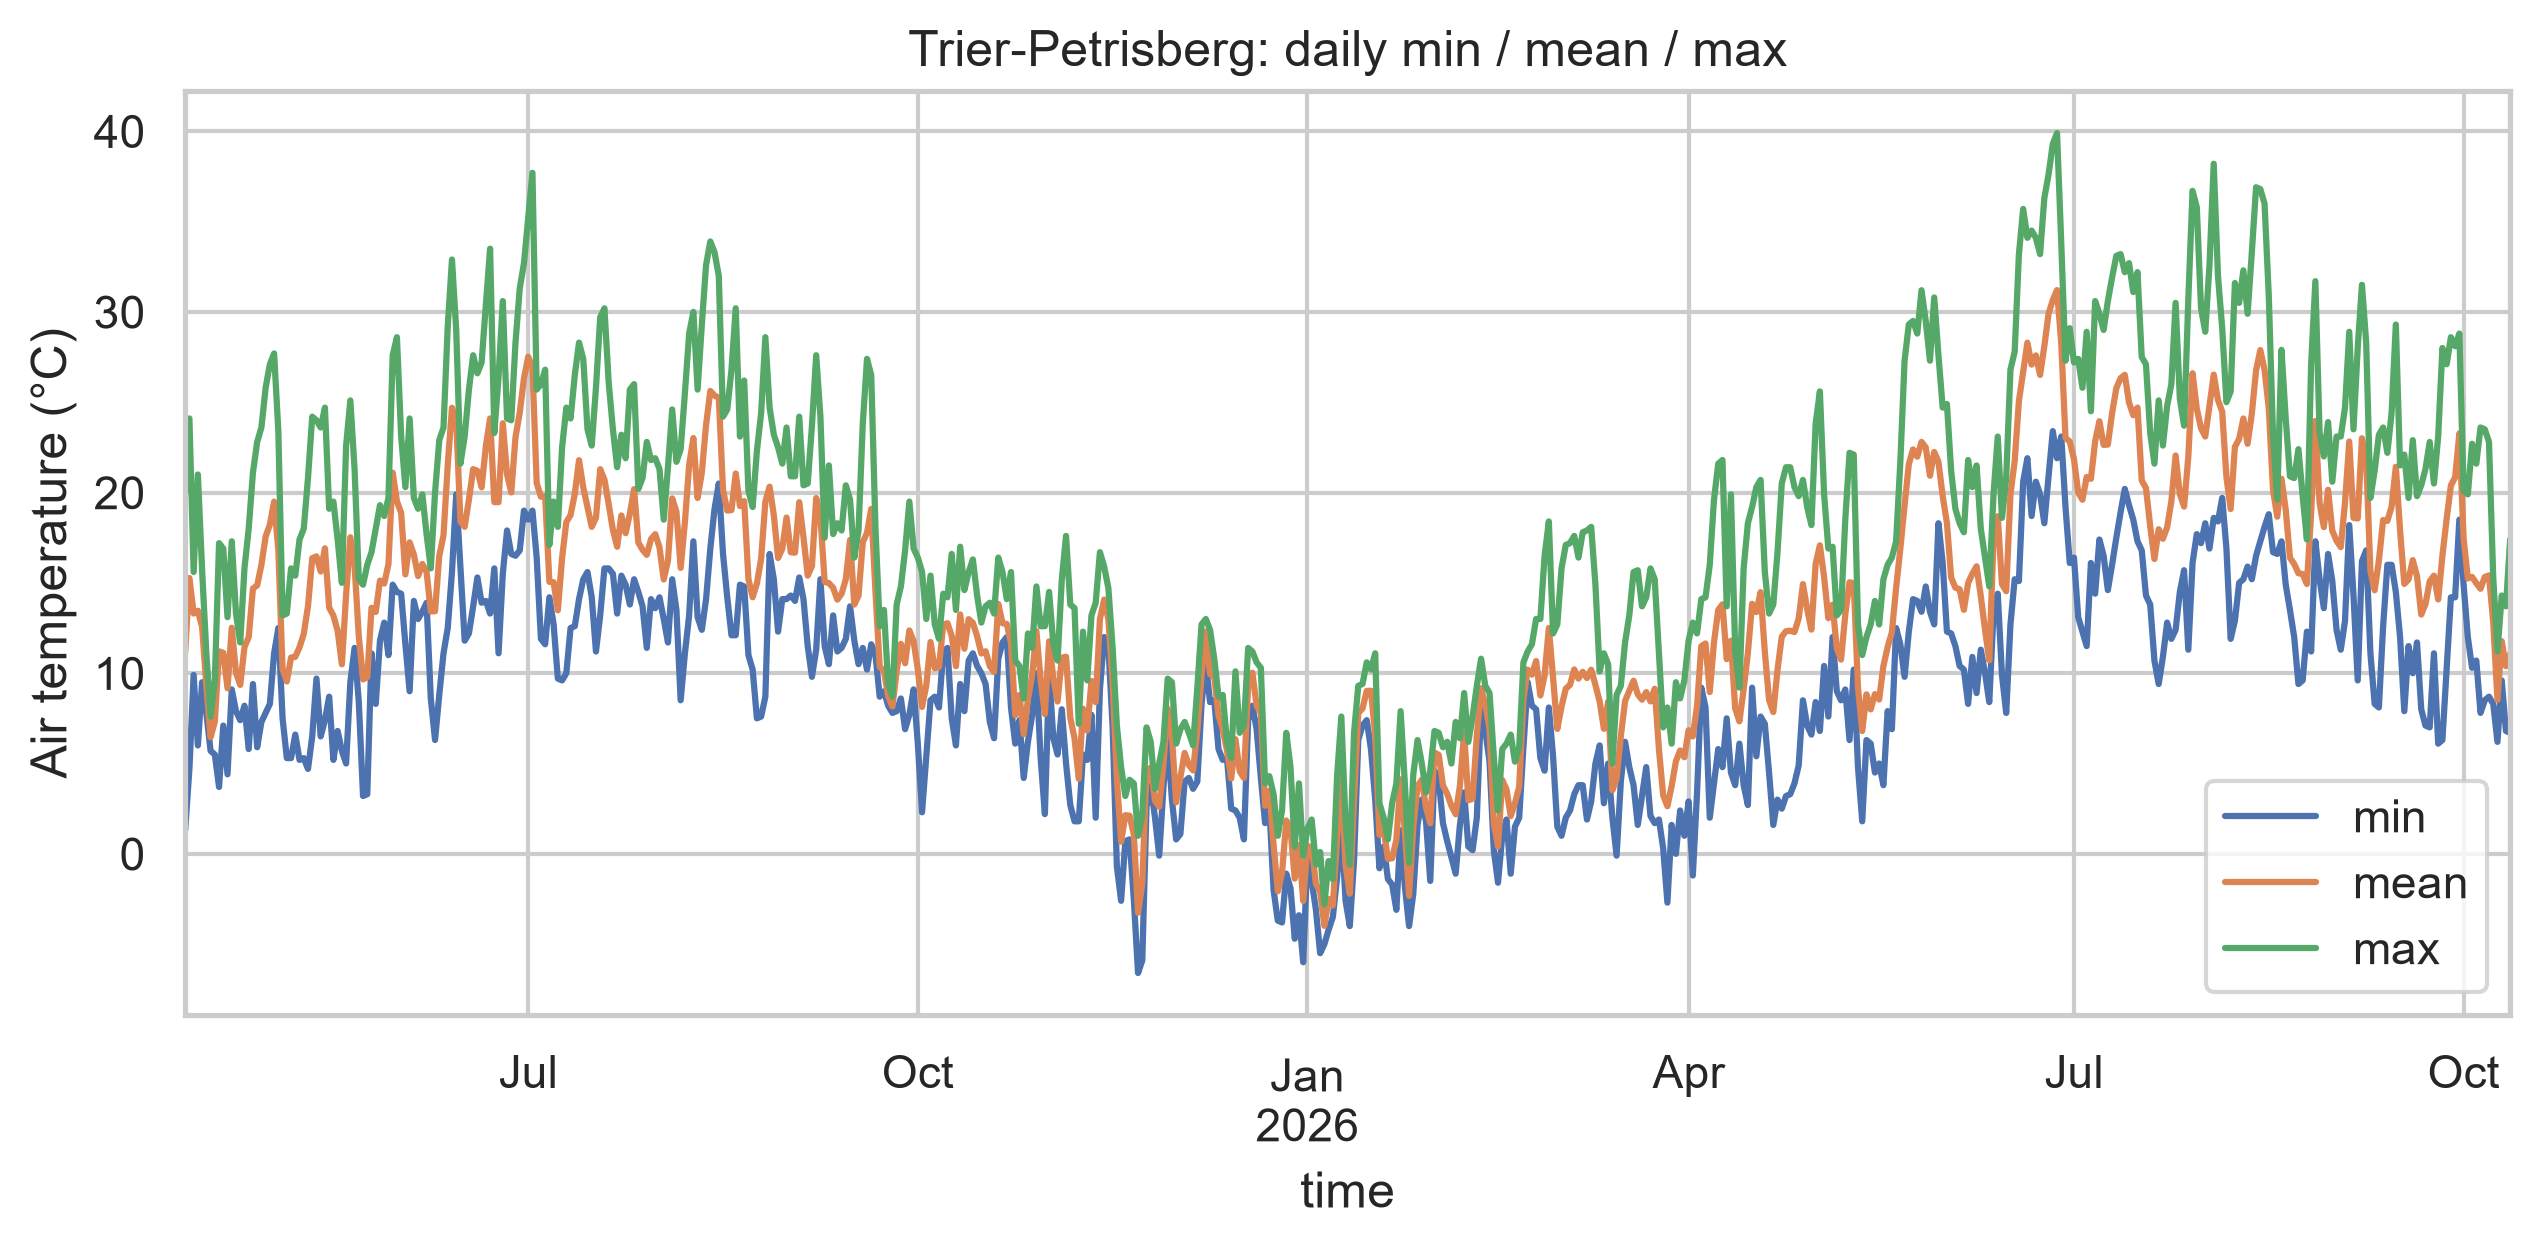
\includegraphics[keepaspectratio]{notebooks/02-eda_files/figure-pdf/cell-7-output-1.png}}

\textbf{Discussion.} With a time index, pandas offers powerful
operations: \texttt{resample("D")} aggregates hourly values to days, and
we can compute several statistics at once. The plot shows the seasonal
cycle and the day-to-day weather variability. Note the time zone: the
DWD files of this product use UTC. When you combine such data with local
production data, time zones and daylight saving time must be handled
explicitly -- a common source of one-hour shifts.

The output above also reports a few missing hours -- the former
\texttt{-999} codes, now \texttt{NaN}. Why they are missing is
documented in the metadata file \texttt{Metadaten\_Fehldaten\_…} in the
archive. Reading it is the first step before choosing a treatment (see
\emph{Missing data} above).

\section{Live coding: energy use of a low-energy
house}\label{live-coding-energy-use-of-a-low-energy-house}

The dataset was recorded in a low-energy house in Belgium. A wireless
sensor network measured temperature and humidity in nine rooms every 10
minutes for about 4.5 months; the electricity consumption of the
appliances was logged by an energy meter, and outdoor weather was taken
from a nearby airport. Key columns:

\begin{longtable}[]{@{}
  >{\raggedright\arraybackslash}p{(\linewidth - 4\tabcolsep) * \real{0.3333}}
  >{\raggedright\arraybackslash}p{(\linewidth - 4\tabcolsep) * \real{0.3333}}
  >{\raggedright\arraybackslash}p{(\linewidth - 4\tabcolsep) * \real{0.3333}}@{}}
\toprule\noalign{}
\begin{minipage}[b]{\linewidth}\raggedright
Column
\end{minipage} & \begin{minipage}[b]{\linewidth}\raggedright
Meaning
\end{minipage} & \begin{minipage}[b]{\linewidth}\raggedright
Unit
\end{minipage} \\
\midrule\noalign{}
\endhead
\bottomrule\noalign{}
\endlastfoot
\texttt{Appliances} & energy use of appliances in the 10-minute interval
& Wh \\
\texttt{lights} & energy use of light fixtures & Wh \\
\texttt{T1} \ldots{} \texttt{T9}, \texttt{RH\_1} \ldots{} \texttt{RH\_9}
& temperature and relative humidity in the rooms & °C, \% \\
\texttt{T\_out}, \texttt{RH\_out}, \texttt{Windspeed}, \ldots{} &
outdoor weather & various \\
\texttt{rv1}, \texttt{rv2} & random variables, added deliberately by the
authors & -- \\
\end{longtable}

The two random variables are a nice feature of this dataset: a sound
analysis should find that they carry no information.

\begin{Shaded}
\begin{Highlighting}[]
\ImportTok{from}\NormalTok{ ucimlrepo }\ImportTok{import}\NormalTok{ fetch\_ucirepo}

\NormalTok{appl }\OperatorTok{=}\NormalTok{ fetch\_ucirepo(}\BuiltInTok{id}\OperatorTok{=}\DecValTok{374}\NormalTok{)}
\NormalTok{energy }\OperatorTok{=}\NormalTok{ appl.data.original.copy()}

\CommentTok{\# Time stamps come in many formats. Look at the raw strings first ...}
\NormalTok{raw }\OperatorTok{=}\NormalTok{ energy[}\StringTok{"date"}\NormalTok{].astype(}\BuiltInTok{str}\NormalTok{).}\BuiltInTok{str}\NormalTok{.strip()}
\BuiltInTok{print}\NormalTok{(}\StringTok{"Raw time stamps:"}\NormalTok{, raw.iloc[:}\DecValTok{3}\NormalTok{].tolist())}

\CommentTok{\# ... and parse them with an explicit format instead of letting pandas guess.}
\KeywordTok{def}\NormalTok{ parse\_timestamps(s, formats}\OperatorTok{=}\NormalTok{(}\StringTok{"\%Y{-}\%m{-}}\SpecialCharTok{\%d}\StringTok{ \%H:\%M:\%S"}\NormalTok{, }\StringTok{"\%Y{-}\%m{-}}\SpecialCharTok{\%d}\StringTok{\%H:\%M:\%S"}\NormalTok{, }\StringTok{"\%Y{-}\%m{-}}\SpecialCharTok{\%d}\StringTok{ \%H:\%M"}\NormalTok{, }\StringTok{"}\SpecialCharTok{\%d}\StringTok{{-}\%m{-}\%Y \%H:\%M:\%S"}\NormalTok{,}
                                 \StringTok{"}\SpecialCharTok{\%d}\StringTok{{-}\%m{-}\%Y \%H:\%M"}\NormalTok{, }\StringTok{"}\SpecialCharTok{\%d}\StringTok{/\%m/\%Y \%H:\%M"}\NormalTok{, }\StringTok{"\%m/}\SpecialCharTok{\%d}\StringTok{/\%Y \%H:\%M"}\NormalTok{,}
                                 \StringTok{"}\SpecialCharTok{\%d}\StringTok{.\%m.\%Y \%H:\%M"}\NormalTok{)):}
    \ControlFlowTok{for}\NormalTok{ fmt }\KeywordTok{in}\NormalTok{ formats:}
\NormalTok{        t }\OperatorTok{=}\NormalTok{ pd.to\_datetime(s, }\BuiltInTok{format}\OperatorTok{=}\NormalTok{fmt, errors}\OperatorTok{=}\StringTok{"coerce"}\NormalTok{)}
        \ControlFlowTok{if}\NormalTok{ t.notna().}\BuiltInTok{all}\NormalTok{():}
            \BuiltInTok{print}\NormalTok{(}\StringTok{"Time stamp format:"}\NormalTok{, fmt)}
            \ControlFlowTok{return}\NormalTok{ t}
\NormalTok{    bad }\OperatorTok{=}\NormalTok{ s[pd.to\_datetime(s, }\BuiltInTok{format}\OperatorTok{=}\StringTok{"mixed"}\NormalTok{, errors}\OperatorTok{=}\StringTok{"coerce"}\NormalTok{).isna()]}
    \ControlFlowTok{raise} \PreprocessorTok{ValueError}\NormalTok{(}\SpecialStringTok{f"Unknown time stamp format, e.g. }\SpecialCharTok{\{}\NormalTok{bad}\SpecialCharTok{.}\NormalTok{iloc[:}\DecValTok{3}\NormalTok{]}\SpecialCharTok{.}\NormalTok{tolist() }\KeywordTok{or}\NormalTok{ s}\SpecialCharTok{.}\NormalTok{iloc[:}\DecValTok{3}\NormalTok{]}\SpecialCharTok{.}\NormalTok{tolist()}\SpecialCharTok{\}}\SpecialStringTok{"}\NormalTok{)}

\NormalTok{energy[}\StringTok{"date"}\NormalTok{] }\OperatorTok{=}\NormalTok{ parse\_timestamps(raw)}
\NormalTok{energy }\OperatorTok{=}\NormalTok{ energy.set\_index(}\StringTok{"date"}\NormalTok{).sort\_index()}
\BuiltInTok{print}\NormalTok{(energy.shape, energy.index.}\BuiltInTok{min}\NormalTok{(), }\StringTok{"to"}\NormalTok{, energy.index.}\BuiltInTok{max}\NormalTok{())}
\BuiltInTok{print}\NormalTok{(}\StringTok{"Missing values:"}\NormalTok{, energy.isna().}\BuiltInTok{sum}\NormalTok{().}\BuiltInTok{sum}\NormalTok{())}
\BuiltInTok{print}\NormalTok{(}\StringTok{"Regular 10{-}min grid:"}\NormalTok{, (energy.index.to\_series().diff().dropna() }\OperatorTok{==}\NormalTok{ pd.Timedelta(}\StringTok{"10min"}\NormalTok{)).}\BuiltInTok{all}\NormalTok{())}
\end{Highlighting}
\end{Shaded}

\begin{verbatim}
Raw time stamps: ['2016-01-1117:00:00', '2016-01-1117:10:00', '2016-01-1117:20:00']
Time stamp format: %Y-%m-%d%H:%M:%S
(19735, 28) 2016-01-11 17:00:00 to 2016-05-27 18:00:00
Missing values: 0
Regular 10-min grid: True
\end{verbatim}

\begin{tcolorbox}[enhanced jigsaw, colframe=quarto-callout-warning-color-frame, toprule=.15mm, rightrule=.15mm, title=\textcolor{quarto-callout-warning-color}{\faExclamationTriangle}\hspace{0.5em}{Pitfall: letting the software guess date formats}, colbacktitle=quarto-callout-warning-color!10!white, left=2mm, titlerule=0mm, bottomtitle=1mm, toptitle=1mm, opacityback=0, bottomrule=.15mm, breakable, arc=.35mm, opacitybacktitle=0.6, colback=white, coltitle=black, leftrule=.75mm]

Is \texttt{03/04/2016} the 3rd of April or the 4th of March? If you let
pandas guess, it may parse some time stamps one way and others the other
way -- or fail on a single unusual entry. Always look at the raw strings
and give the format explicitly. Because the measurement period contains
days after the 12th, only the correct order of day and month can parse
\emph{all} time stamps -- the helper above uses exactly this check.

\end{tcolorbox}

A real-world surprise: in the version of this dataset served by the UCI
repository, date and time are glued together without a space
(\texttt{2016-01-1117:00:00} for 11 January 2016, 17:00). pandas cannot
guess this format -- but the explicit format
\texttt{\%Y-\%m-\%d\%H:\%M:\%S} reads it without problems.

Checking that the time index is regular is a quick but important test.
Gaps in the time grid are ``hidden'' missing values: \texttt{isna()}
does not see them because the rows do not exist at all.

\subsection{The target variable: appliance energy
use}\label{the-target-variable-appliance-energy-use}

\begin{Shaded}
\begin{Highlighting}[]
\NormalTok{fig, axes }\OperatorTok{=}\NormalTok{ plt.subplots(}\DecValTok{1}\NormalTok{, }\DecValTok{2}\NormalTok{, figsize}\OperatorTok{=}\NormalTok{(}\DecValTok{12}\NormalTok{, }\DecValTok{4}\NormalTok{))}
\NormalTok{sns.histplot(energy[}\StringTok{"Appliances"}\NormalTok{], bins}\OperatorTok{=}\DecValTok{60}\NormalTok{, ax}\OperatorTok{=}\NormalTok{axes[}\DecValTok{0}\NormalTok{])}
\NormalTok{axes[}\DecValTok{0}\NormalTok{].}\BuiltInTok{set}\NormalTok{(xlabel}\OperatorTok{=}\StringTok{"Appliances (Wh per 10 min)"}\NormalTok{)}
\NormalTok{sns.boxplot(x}\OperatorTok{=}\NormalTok{energy[}\StringTok{"Appliances"}\NormalTok{], ax}\OperatorTok{=}\NormalTok{axes[}\DecValTok{1}\NormalTok{])}
\NormalTok{axes[}\DecValTok{1}\NormalTok{].}\BuiltInTok{set}\NormalTok{(xlabel}\OperatorTok{=}\StringTok{"Appliances (Wh per 10 min)"}\NormalTok{)}
\NormalTok{plt.tight\_layout()}\OperatorTok{;}\NormalTok{ plt.show()}
\NormalTok{energy[}\StringTok{"Appliances"}\NormalTok{].describe().}\BuiltInTok{round}\NormalTok{(}\DecValTok{1}\NormalTok{)}
\end{Highlighting}
\end{Shaded}

\pandocbounded{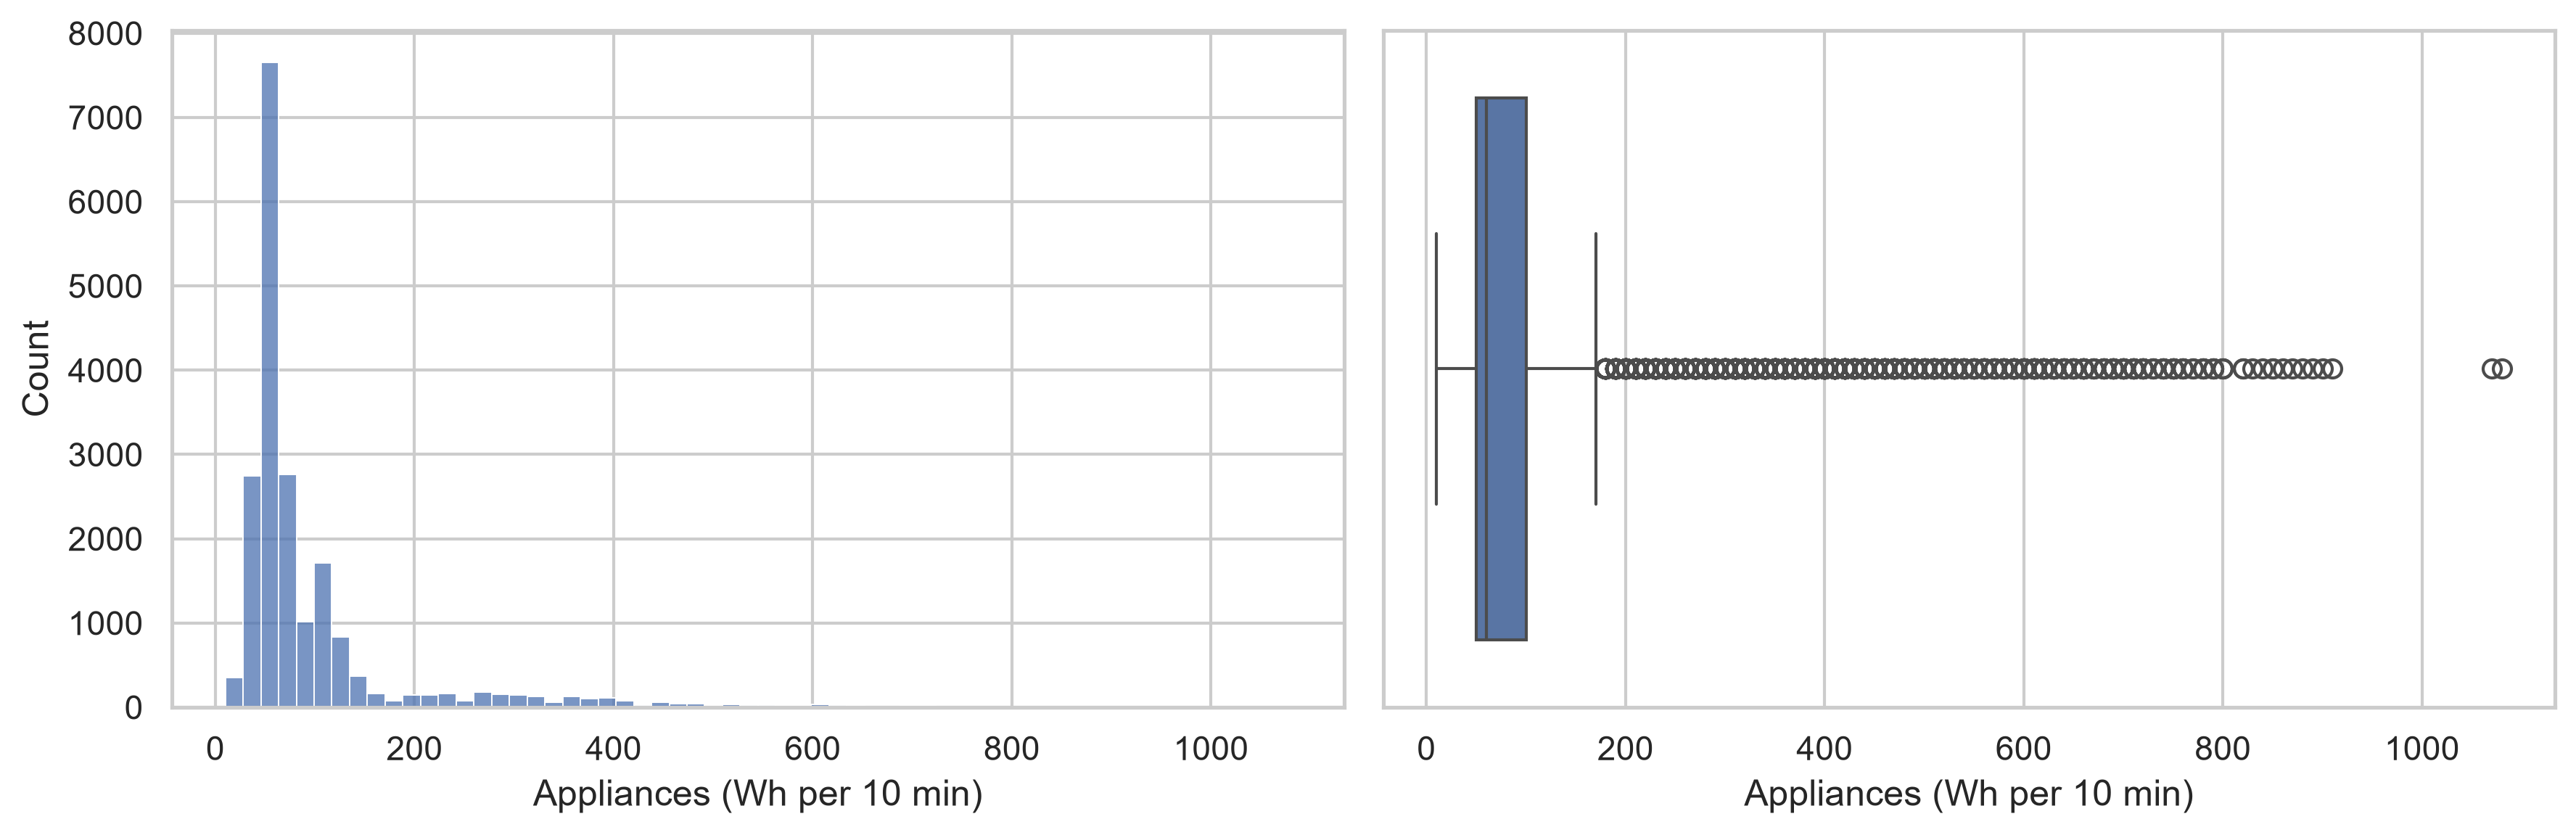
\includegraphics[keepaspectratio]{notebooks/02-eda_files/figure-pdf/cell-9-output-1.png}}

\begin{verbatim}
count    19735.0
mean        97.7
std        102.5
min         10.0
25%         50.0
50%         60.0
75%        100.0
max       1080.0
Name: Appliances, dtype: float64
\end{verbatim}

\textbf{Discussion.} The distribution is strongly \textbf{right-skewed}:
most of the time the consumption is low (base load from fridge,
standby), but occasionally it rises sharply (cooking, washing machine).
Consequently, the mean is clearly larger than the median, and the box
plot flags many points as ``outliers''. Here these are not measurement
errors but real usage events -- deleting them would remove the most
interesting part of the data.

For skewed, positive quantities a \textbf{log transformation} often
helps: it makes the distribution more symmetric and turns multiplicative
effects into additive ones.

\begin{Shaded}
\begin{Highlighting}[]
\NormalTok{fig, axes }\OperatorTok{=}\NormalTok{ plt.subplots(}\DecValTok{2}\NormalTok{, }\DecValTok{1}\NormalTok{, figsize}\OperatorTok{=}\NormalTok{(}\DecValTok{10}\NormalTok{, }\DecValTok{6}\NormalTok{), sharex}\OperatorTok{=}\VariableTok{True}\NormalTok{)}
\NormalTok{energy[}\StringTok{"Appliances"}\NormalTok{].plot(ax}\OperatorTok{=}\NormalTok{axes[}\DecValTok{0}\NormalTok{], lw}\OperatorTok{=}\FloatTok{0.3}\NormalTok{, alpha}\OperatorTok{=}\FloatTok{0.6}\NormalTok{, label}\OperatorTok{=}\StringTok{"10 min"}\NormalTok{)}
\NormalTok{energy[}\StringTok{"Appliances"}\NormalTok{].rolling(}\StringTok{"1D"}\NormalTok{).mean().plot(ax}\OperatorTok{=}\NormalTok{axes[}\DecValTok{0}\NormalTok{], color}\OperatorTok{=}\StringTok{"k"}\NormalTok{, label}\OperatorTok{=}\StringTok{"24 h rolling mean"}\NormalTok{)}
\NormalTok{axes[}\DecValTok{0}\NormalTok{].}\BuiltInTok{set}\NormalTok{(ylabel}\OperatorTok{=}\StringTok{"Appliances (Wh)"}\NormalTok{)}\OperatorTok{;}\NormalTok{ axes[}\DecValTok{0}\NormalTok{].legend()}
\NormalTok{energy[[}\StringTok{"T1"}\NormalTok{, }\StringTok{"T\_out"}\NormalTok{]].resample(}\StringTok{"h"}\NormalTok{).mean().plot(ax}\OperatorTok{=}\NormalTok{axes[}\DecValTok{1}\NormalTok{])}
\NormalTok{axes[}\DecValTok{1}\NormalTok{].}\BuiltInTok{set}\NormalTok{(ylabel}\OperatorTok{=}\StringTok{"Temperature (°C)"}\NormalTok{)}
\NormalTok{plt.show()}
\end{Highlighting}
\end{Shaded}

\pandocbounded{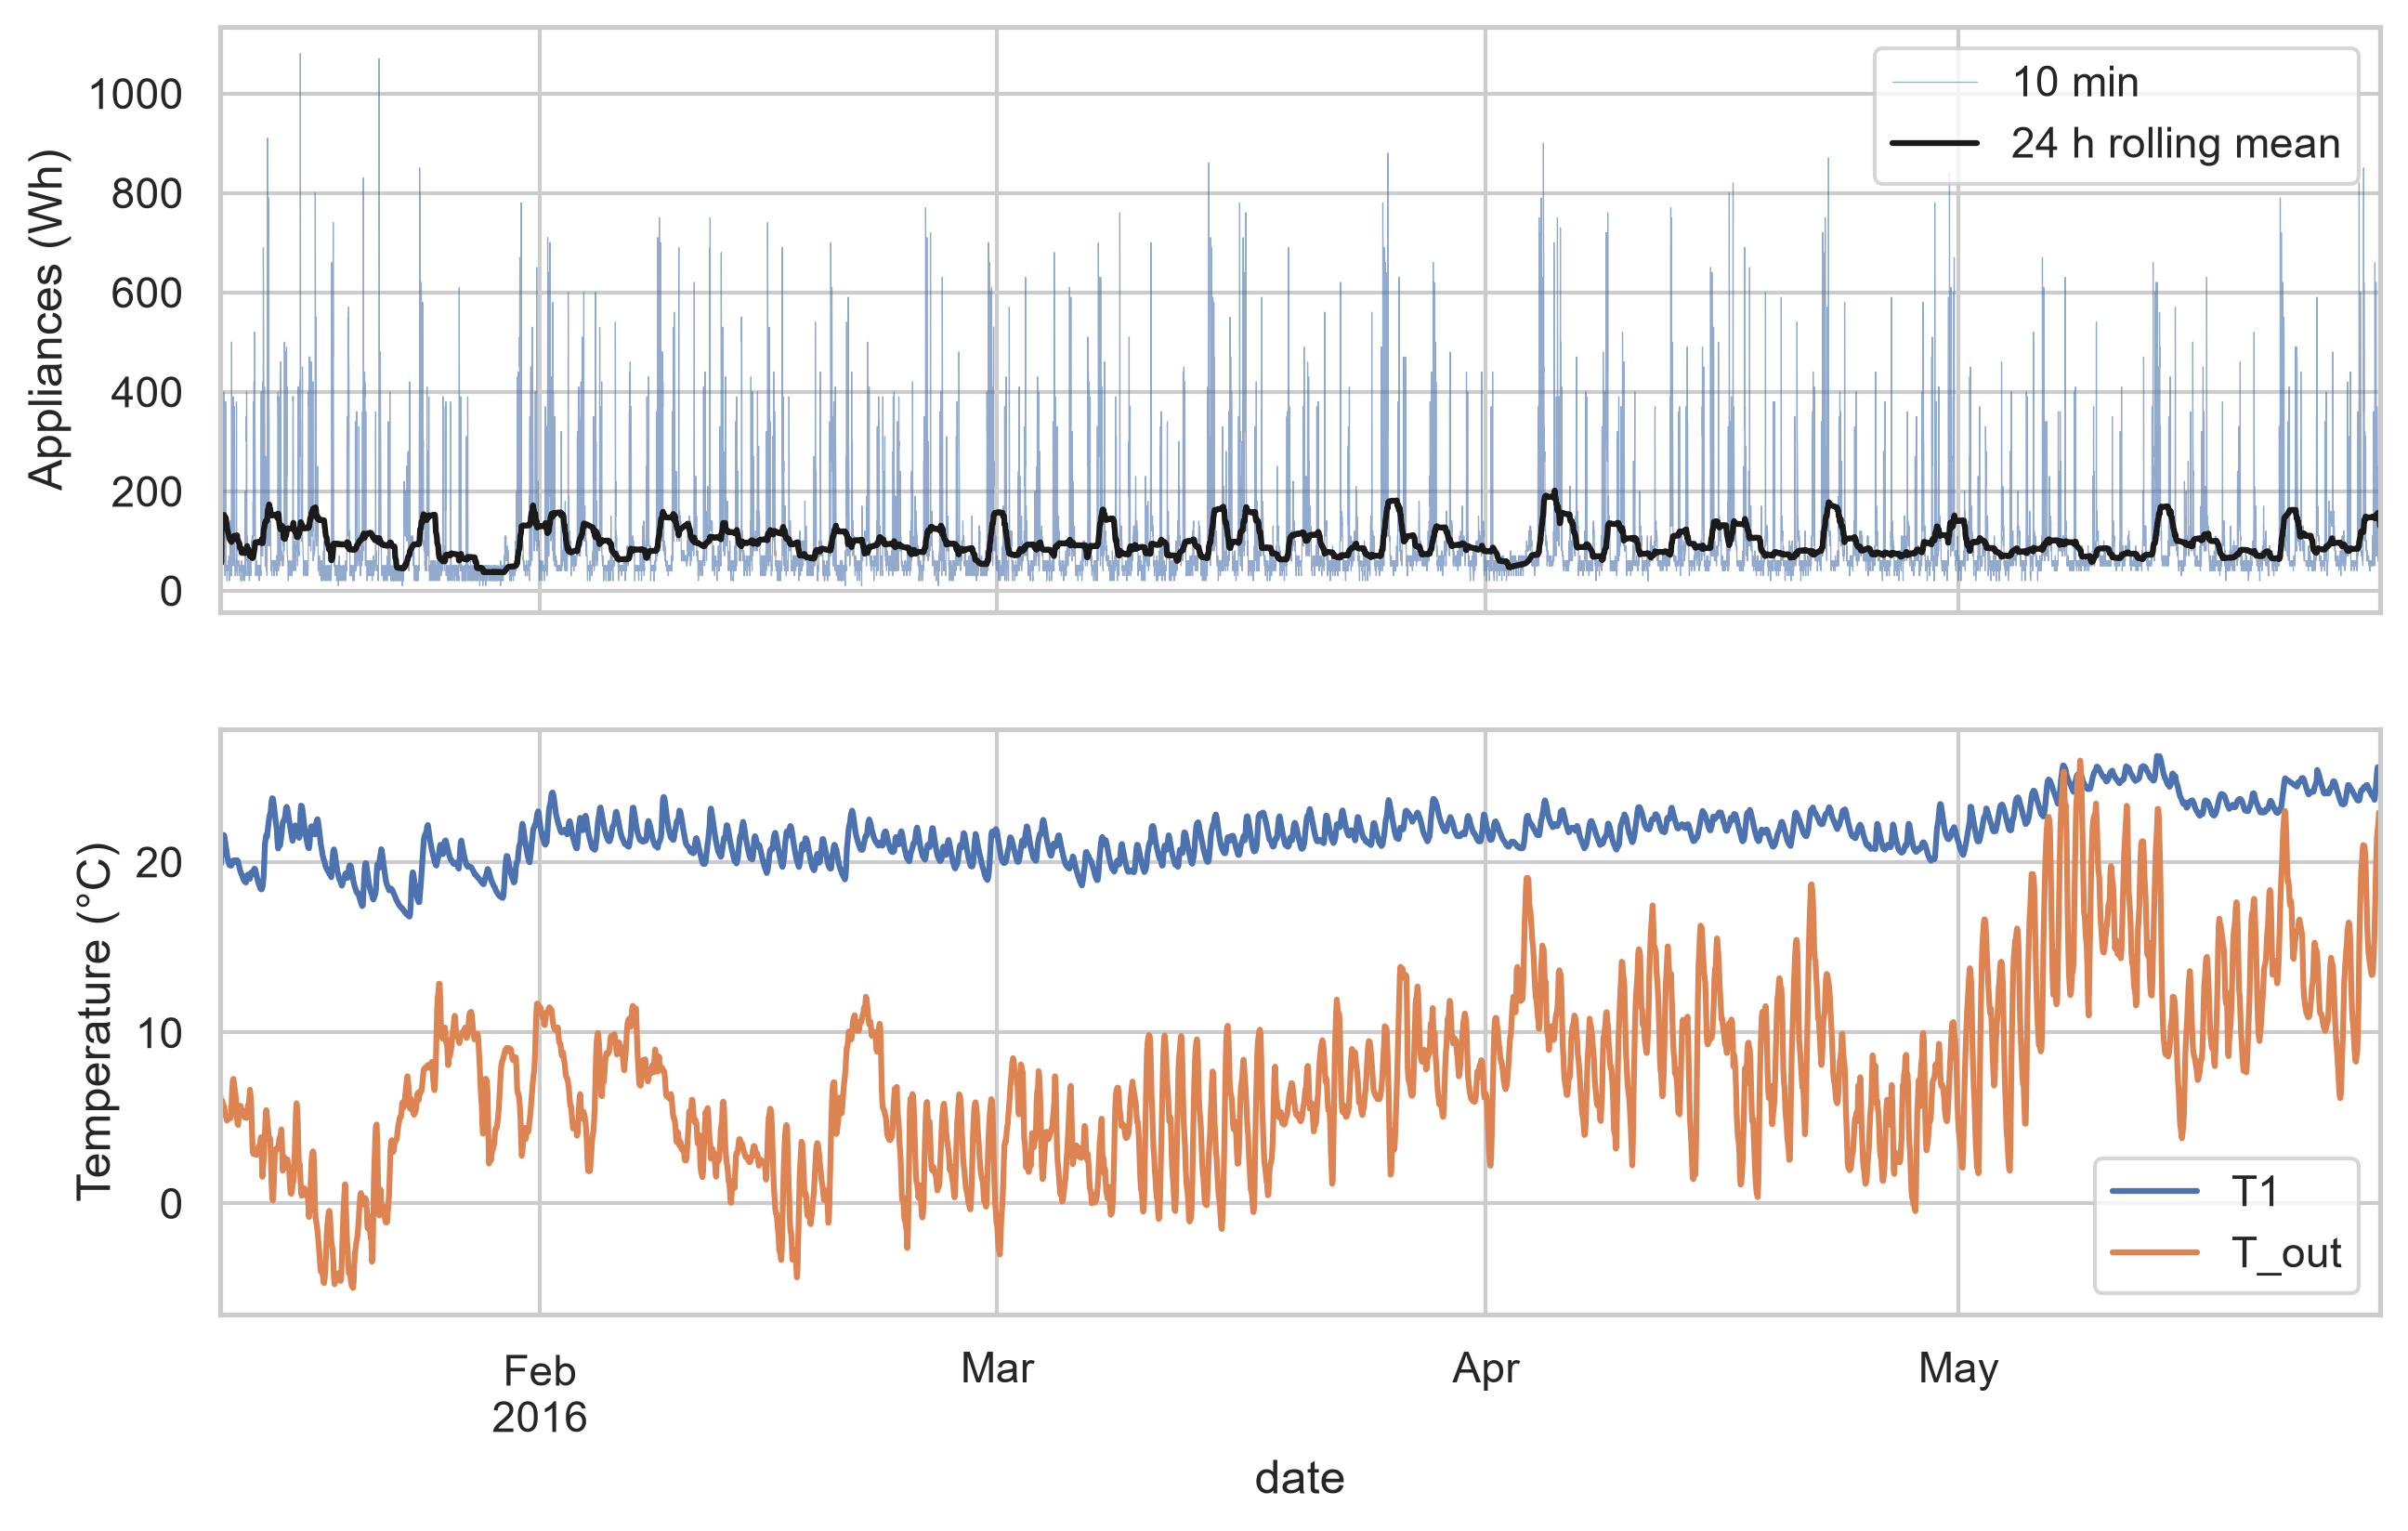
\includegraphics[keepaspectratio]{notebooks/02-eda_files/figure-pdf/cell-10-output-1.png}}

A \textbf{rolling mean} smooths short-term fluctuations and reveals the
level over time. Indoor temperature \texttt{T1} is much more stable than
the outdoor temperature -- as expected for a well-insulated building.

\subsection{Daily and weekly patterns}\label{daily-and-weekly-patterns}

Consumption depends on human behaviour, so we expect patterns over the
hour of the day and the day of the week. A heatmap shows both at once:

\begin{Shaded}
\begin{Highlighting}[]
\NormalTok{profile }\OperatorTok{=}\NormalTok{ energy.groupby([energy.index.dayofweek, energy.index.hour])[}\StringTok{"Appliances"}\NormalTok{].mean().unstack(}\DecValTok{0}\NormalTok{)}
\NormalTok{sns.heatmap(profile, cmap}\OperatorTok{=}\StringTok{"viridis"}\NormalTok{, cbar\_kws}\OperatorTok{=}\NormalTok{\{}\StringTok{"label"}\NormalTok{: }\StringTok{"mean Appliances (Wh)"}\NormalTok{\})}
\NormalTok{plt.xlabel(}\StringTok{"Day of week (0 = Monday)"}\NormalTok{)}\OperatorTok{;}\NormalTok{ plt.ylabel(}\StringTok{"Hour of day"}\NormalTok{)}
\NormalTok{plt.show()}
\end{Highlighting}
\end{Shaded}

\pandocbounded{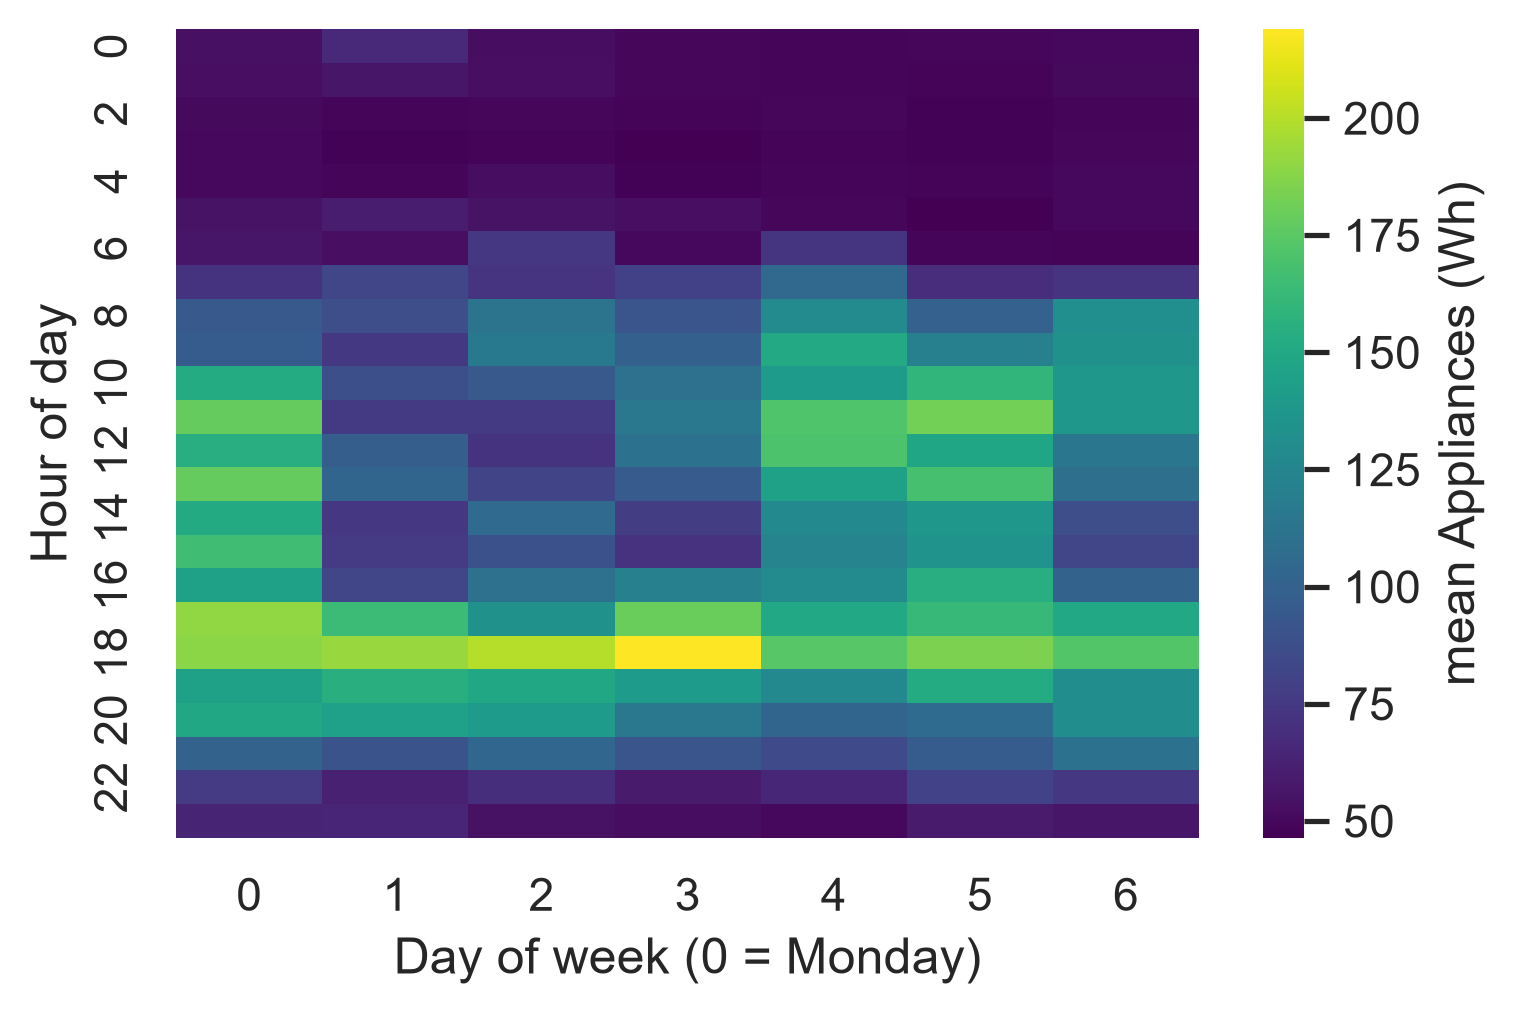
\includegraphics[keepaspectratio]{notebooks/02-eda_files/figure-pdf/cell-11-output-1.png}}

\textbf{Discussion.} Low consumption at night, a rise in the morning and
a peak in the evening hours -- a typical residential profile. Such
patterns are important for later modelling: hour of day and weekday are
strong features for forecasting (Chapter 11).

\subsection{Outliers: IQR rule and robust
z-score}\label{outliers-iqr-rule-and-robust-z-score}

\begin{tcolorbox}[enhanced jigsaw, colframe=quarto-callout-note-color-frame, toprule=.15mm, rightrule=.15mm, title=\textcolor{quarto-callout-note-color}{\faInfo}\hspace{0.5em}{Definition: Outlier rules}, colbacktitle=quarto-callout-note-color!10!white, left=2mm, titlerule=0mm, bottomtitle=1mm, toptitle=1mm, opacityback=0, bottomrule=.15mm, breakable, arc=.35mm, opacitybacktitle=0.6, colback=white, coltitle=black, leftrule=.75mm]

\begin{itemize}
\tightlist
\item
  \textbf{IQR rule (Tukey):} a value is flagged if it lies below
  \(Q_1 - 1.5\,\text{IQR}\) or above \(Q_3 + 1.5\,\text{IQR}\). These
  are the whiskers of the box plot.
\item
  \textbf{Robust z-score:}
  \(z_i = \dfrac{x_i - \tilde x}{1.4826 \cdot \text{MAD}}\), flag if
  \(|z_i| > 3.5\), where \(\tilde x\) is the median. The factor 1.4826
  makes MAD comparable to the standard deviation for normally
  distributed data.
\end{itemize}

\end{tcolorbox}

The ordinary z-score \((x_i - \bar x)/s\) is less suitable for outlier
detection: the outliers themselves inflate \(\bar x\) and \(s\) and can
hide each other (\emph{masking}).

\begin{Shaded}
\begin{Highlighting}[]
\KeywordTok{def}\NormalTok{ iqr\_outliers(x, k}\OperatorTok{=}\FloatTok{1.5}\NormalTok{):}
\NormalTok{    q1, q3 }\OperatorTok{=}\NormalTok{ x.quantile([}\FloatTok{0.25}\NormalTok{, }\FloatTok{0.75}\NormalTok{])}
    \ControlFlowTok{return}\NormalTok{ (x }\OperatorTok{\textless{}}\NormalTok{ q1 }\OperatorTok{{-}}\NormalTok{ k }\OperatorTok{*}\NormalTok{ (q3 }\OperatorTok{{-}}\NormalTok{ q1)) }\OperatorTok{|}\NormalTok{ (x }\OperatorTok{\textgreater{}}\NormalTok{ q3 }\OperatorTok{+}\NormalTok{ k }\OperatorTok{*}\NormalTok{ (q3 }\OperatorTok{{-}}\NormalTok{ q1))}

\KeywordTok{def}\NormalTok{ robust\_z(x):}
\NormalTok{    mad }\OperatorTok{=}\NormalTok{ (x }\OperatorTok{{-}}\NormalTok{ x.median()).}\BuiltInTok{abs}\NormalTok{().median()}
    \ControlFlowTok{return}\NormalTok{ (x }\OperatorTok{{-}}\NormalTok{ x.median()) }\OperatorTok{/}\NormalTok{ (}\FloatTok{1.4826} \OperatorTok{*}\NormalTok{ mad)}

\ControlFlowTok{for}\NormalTok{ col }\KeywordTok{in}\NormalTok{ [}\StringTok{"Appliances"}\NormalTok{, }\StringTok{"T1"}\NormalTok{, }\StringTok{"T\_out"}\NormalTok{, }\StringTok{"RH\_1"}\NormalTok{]:}
\NormalTok{    x }\OperatorTok{=}\NormalTok{ energy[col]}
    \BuiltInTok{print}\NormalTok{(}\SpecialStringTok{f"}\SpecialCharTok{\{}\NormalTok{col}\SpecialCharTok{:11s\}}\SpecialStringTok{ IQR rule: }\SpecialCharTok{\{}\NormalTok{iqr\_outliers(x)}\SpecialCharTok{.}\NormalTok{mean()}\SpecialCharTok{:6.1\%\}}\SpecialStringTok{   |robust z| \textgreater{} 3.5: }\SpecialCharTok{\{}\NormalTok{(robust\_z(x).}\BuiltInTok{abs}\NormalTok{() }\OperatorTok{\textgreater{}} \FloatTok{3.5}\NormalTok{)}\SpecialCharTok{.}\NormalTok{mean()}\SpecialCharTok{:6.1\%\}}\SpecialStringTok{"}\NormalTok{)}
\end{Highlighting}
\end{Shaded}

\begin{verbatim}
Appliances  IQR rule:  10.8%   |robust z| > 3.5:  11.2%
T1          IQR rule:   2.6%   |robust z| > 3.5:   0.2%
T_out       IQR rule:   2.2%   |robust z| > 3.5:   0.3%
RH_1        IQR rule:   0.7%   |robust z| > 3.5:   0.2%
\end{verbatim}

For the room temperature and humidity, very few values are flagged; for
\texttt{Appliances}, many. This confirms that a fixed rule cannot decide
alone: the flags tell us where to \emph{look}, the engineer decides what
the values mean.

\section{Live coding: missing values in semiconductor
manufacturing}\label{live-coding-missing-values-in-semiconductor-manufacturing}

SECOM contains data from a semiconductor manufacturing process: 1,567
production runs, each described by 591 sensor and process measurements,
and a label pass (−1) or fail (1). The sensor names are anonymised. Many
signals have gaps. A small obstacle on the way: in the repository's
metadata the label is not marked as the target variable -- another
example of incomplete metadata. The helper function below therefore
identifies the label column from its values.

\begin{Shaded}
\begin{Highlighting}[]
\KeywordTok{def}\NormalTok{ load\_secom():}
    \CommentTok{"""SECOM: return the process measurements X and the label y ({-}1 = pass, 1 = fail).}

\CommentTok{    In the UCI repository the label is not marked as target variable, so we find it}
\CommentTok{    ourselves: the only numeric column whose values are exactly {-}1 and 1.}
\CommentTok{    """}
\NormalTok{    df }\OperatorTok{=}\NormalTok{ fetch\_ucirepo(}\BuiltInTok{id}\OperatorTok{=}\DecValTok{179}\NormalTok{).data.original}
\NormalTok{    num }\OperatorTok{=}\NormalTok{ df.select\_dtypes(}\StringTok{"number"}\NormalTok{)}
\NormalTok{    labels }\OperatorTok{=}\NormalTok{ [c }\ControlFlowTok{for}\NormalTok{ c }\KeywordTok{in}\NormalTok{ num.columns }\ControlFlowTok{if} \BuiltInTok{set}\NormalTok{(num[c].dropna().unique()) }\OperatorTok{==}\NormalTok{ \{}\OperatorTok{{-}}\DecValTok{1}\NormalTok{, }\DecValTok{1}\NormalTok{\}]}
    \ControlFlowTok{if} \BuiltInTok{len}\NormalTok{(labels) }\OperatorTok{!=} \DecValTok{1}\NormalTok{:}
\NormalTok{        labels }\OperatorTok{=}\NormalTok{ [c }\ControlFlowTok{for}\NormalTok{ c }\KeywordTok{in}\NormalTok{ df.columns }\ControlFlowTok{if} \BuiltInTok{any}\NormalTok{(k }\KeywordTok{in} \BuiltInTok{str}\NormalTok{(c).lower() }\ControlFlowTok{for}\NormalTok{ k }\KeywordTok{in}\NormalTok{ (}\StringTok{"pass"}\NormalTok{, }\StringTok{"fail"}\NormalTok{, }\StringTok{"label"}\NormalTok{))]}
    \ControlFlowTok{assert} \BuiltInTok{len}\NormalTok{(labels) }\OperatorTok{==} \DecValTok{1}\NormalTok{, }\SpecialStringTok{f"Label column not found unambiguously: }\SpecialCharTok{\{}\NormalTok{labels}\SpecialCharTok{\}}\SpecialStringTok{"}
\NormalTok{    y }\OperatorTok{=}\NormalTok{ df[labels[}\DecValTok{0}\NormalTok{]].astype(}\BuiltInTok{int}\NormalTok{)}
\NormalTok{    X }\OperatorTok{=}\NormalTok{ num.drop(columns}\OperatorTok{=}\NormalTok{labels, errors}\OperatorTok{=}\StringTok{"ignore"}\NormalTok{)}
    \BuiltInTok{print}\NormalTok{(}\SpecialStringTok{f"Label column: }\SpecialCharTok{\{}\NormalTok{labels[}\DecValTok{0}\NormalTok{]}\SpecialCharTok{!r\}}\SpecialStringTok{, measurement columns: }\SpecialCharTok{\{}\NormalTok{X}\SpecialCharTok{.}\NormalTok{shape[}\DecValTok{1}\NormalTok{]}\SpecialCharTok{\}}\SpecialStringTok{, "}
          \SpecialStringTok{f"ignored non{-}numeric columns: }\SpecialCharTok{\{}\NormalTok{[c }\ControlFlowTok{for}\NormalTok{ c }\KeywordTok{in}\NormalTok{ df.columns }\ControlFlowTok{if}\NormalTok{ c }\KeywordTok{not} \KeywordTok{in}\NormalTok{ num.columns]}\SpecialCharTok{\}}\SpecialStringTok{"}\NormalTok{)}
    \ControlFlowTok{return}\NormalTok{ X, y}

\NormalTok{X, y }\OperatorTok{=}\NormalTok{ load\_secom()}
\NormalTok{missing }\OperatorTok{=}\NormalTok{ X.isna().mean().sort\_values(ascending}\OperatorTok{=}\VariableTok{False}\NormalTok{)}
\BuiltInTok{print}\NormalTok{(}\SpecialStringTok{f"Runs: }\SpecialCharTok{\{}\BuiltInTok{len}\NormalTok{(X)}\SpecialCharTok{\}}\SpecialStringTok{, failed runs: }\SpecialCharTok{\{}\NormalTok{(y }\OperatorTok{==} \DecValTok{1}\NormalTok{)}\SpecialCharTok{.}\BuiltInTok{sum}\NormalTok{()}\SpecialCharTok{\}}\SpecialStringTok{"}\NormalTok{)}
\BuiltInTok{print}\NormalTok{(}\SpecialStringTok{f"Features: }\SpecialCharTok{\{}\NormalTok{X}\SpecialCharTok{.}\NormalTok{shape[}\DecValTok{1}\NormalTok{]}\SpecialCharTok{\}}\SpecialStringTok{, with any missing value: }\SpecialCharTok{\{}\NormalTok{(missing }\OperatorTok{\textgreater{}} \DecValTok{0}\NormalTok{)}\SpecialCharTok{.}\BuiltInTok{sum}\NormalTok{()}\SpecialCharTok{\}}\SpecialStringTok{, "}
      \SpecialStringTok{f"more than 50 \% missing: }\SpecialCharTok{\{}\NormalTok{(missing }\OperatorTok{\textgreater{}} \FloatTok{0.5}\NormalTok{)}\SpecialCharTok{.}\BuiltInTok{sum}\NormalTok{()}\SpecialCharTok{\}}\SpecialStringTok{"}\NormalTok{)}
\NormalTok{missing.plot.hist(bins}\OperatorTok{=}\DecValTok{40}\NormalTok{, xlabel}\OperatorTok{=}\StringTok{"Share of missing values per feature"}\NormalTok{)}
\NormalTok{plt.show()}
\end{Highlighting}
\end{Shaded}

\begin{verbatim}
Label column: 'class', measurement columns: 590, ignored non-numeric columns: ['timestamp']
Runs: 1567, failed runs: 104
Features: 590, with any missing value: 538, more than 50 % missing: 28
\end{verbatim}

\pandocbounded{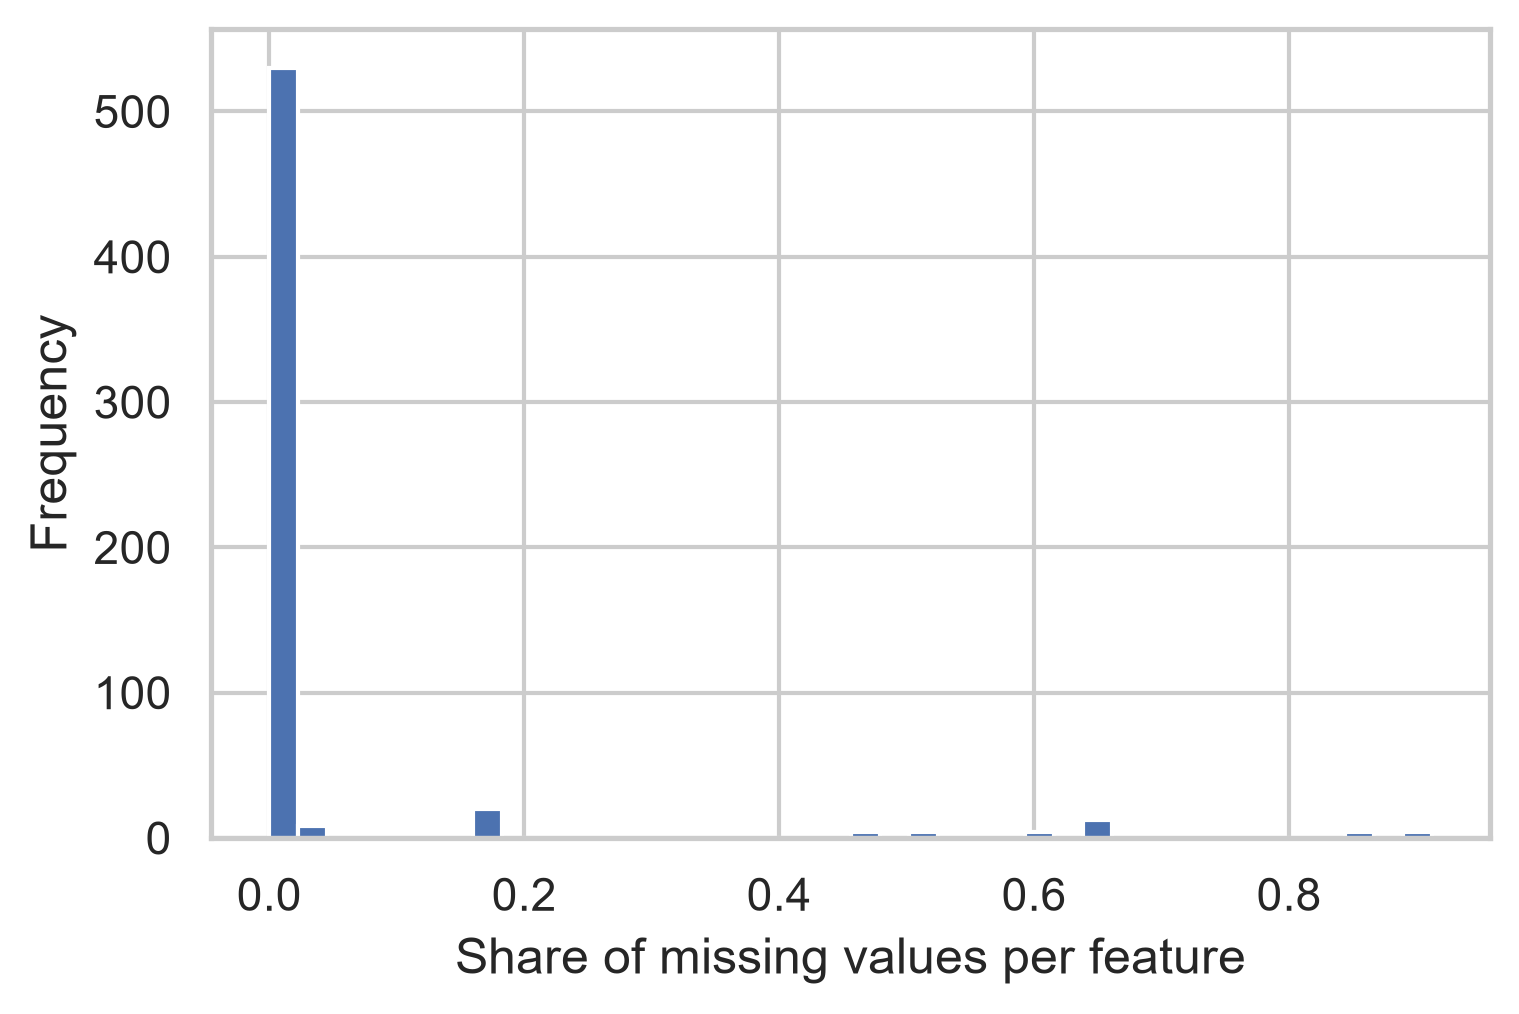
\includegraphics[keepaspectratio]{notebooks/02-eda_files/figure-pdf/cell-13-output-2.png}}

\begin{Shaded}
\begin{Highlighting}[]
\CommentTok{\# Is the missingness itself related to the outcome?}
\NormalTok{miss\_rate }\OperatorTok{=}\NormalTok{ X.isna().mean(axis}\OperatorTok{=}\DecValTok{1}\NormalTok{)}
\BuiltInTok{print}\NormalTok{(miss\_rate.groupby(y).describe().}\BuiltInTok{round}\NormalTok{(}\DecValTok{3}\NormalTok{))}

\CommentTok{\# Constant features carry no information}
\NormalTok{n\_constant }\OperatorTok{=}\NormalTok{ (X.nunique(dropna}\OperatorTok{=}\VariableTok{True}\NormalTok{) }\OperatorTok{\textless{}=} \DecValTok{1}\NormalTok{).}\BuiltInTok{sum}\NormalTok{()}
\BuiltInTok{print}\NormalTok{(}\StringTok{"Constant features:"}\NormalTok{, n\_constant)}
\end{Highlighting}
\end{Shaded}

\begin{verbatim}
        count   mean    std    min    25%    50%    75%    max
class                                                         
-1     1463.0  0.046  0.023  0.007  0.034  0.041  0.054  0.258
 1      104.0  0.043  0.017  0.014  0.034  0.041  0.047  0.108
Constant features: 116
\end{verbatim}

\textbf{Discussion.} Most features are complete or nearly complete, but
a group of features has a large share of missing values -- often entire
sensors that were only recorded for part of the runs. In addition, a
considerable number of features are constant and can be removed without
loss. Comparing the share of missing values between passed and failed
runs is a quick check of whether missingness could be informative
(MAR/MNAR rather than MCAR).

A pragmatic preparation for SECOM, which we will use in Chapter 9:

\begin{enumerate}
\def\labelenumi{\arabic{enumi}.}
\tightlist
\item
  remove constant features,
\item
  remove features with more than 50 \% missing values,
\item
  impute the remaining gaps with the median,
\item
  standardise all features.
\end{enumerate}

\begin{tcolorbox}[enhanced jigsaw, colframe=quarto-callout-warning-color-frame, toprule=.15mm, rightrule=.15mm, title=\textcolor{quarto-callout-warning-color}{\faExclamationTriangle}\hspace{0.5em}{Pitfall: preprocessing before splitting}, colbacktitle=quarto-callout-warning-color!10!white, left=2mm, titlerule=0mm, bottomtitle=1mm, toptitle=1mm, opacityback=0, bottomrule=.15mm, breakable, arc=.35mm, opacitybacktitle=0.6, colback=white, coltitle=black, leftrule=.75mm]

Medians for imputation and means/standard deviations for scaling must be
computed on the \textbf{training data only} and then applied to the test
data. Computing them on the full dataset leaks information from the test
set into the model. In scikit-learn, putting all steps into a
\texttt{Pipeline} prevents this automatically (Chapter 6).

\emph{And how are gaps in the test data filled?} With the
\textbf{training} median as well -- not with a median computed from the
test data. The median is a parameter of the model, just like a
regression coefficient: it is estimated once from the training data and
then applied unchanged to all new data. Three reasons:

\begin{itemize}
\tightlist
\item
  In operation there is no ``test median'': new data often arrive one
  observation at a time -- a single production run, a single sensor
  reading -- and a median cannot be computed from one value.
\item
  The model must always receive the same preprocessing. If a gap was
  filled with 52.3 during training but with 48.9 during testing, the
  model sees inputs it was not trained on.
\item
  A test median would itself be a small leak: the prediction for one
  test point would depend on the other test points.
\end{itemize}

The same holds for scaling, PCA and every other preprocessing step:
\texttt{fit} on the training data, \texttt{transform} on training
\emph{and} test data. If the distribution of new data drifts away from
the training data, the remedy is to monitor the drift and retrain -- not
to compute statistics on the test data. (One legitimate exception: if a
whole batch -- say all wafers of a lot -- is always available at
prediction time, statistics per batch may be used, but then in exactly
the same way during training.)

\end{tcolorbox}

\section{Back to the decision}\label{back-to-the-decision-1}

For a go/no-go recommendation, three questions matter: Are enough
features usable? Are there enough examples of the event we want to
predict? And are the gaps understood? We use simple, transparent
criteria: at least half of the features should be non-constant with at
most 50 \% missing values, and there should be at least 50 failed runs
to learn from.

\begin{Shaded}
\begin{Highlighting}[]
\NormalTok{usable }\OperatorTok{=}\NormalTok{ (X.nunique(dropna}\OperatorTok{=}\VariableTok{True}\NormalTok{) }\OperatorTok{\textgreater{}} \DecValTok{1}\NormalTok{) }\OperatorTok{\&}\NormalTok{ (X.isna().mean() }\OperatorTok{\textless{}=} \FloatTok{0.5}\NormalTok{)}
\NormalTok{n\_fail }\OperatorTok{=} \BuiltInTok{int}\NormalTok{((y }\OperatorTok{==} \DecValTok{1}\NormalTok{).}\BuiltInTok{sum}\NormalTok{())}
\BuiltInTok{print}\NormalTok{(}\SpecialStringTok{f"Usable features: }\SpecialCharTok{\{}\NormalTok{usable}\SpecialCharTok{.}\BuiltInTok{sum}\NormalTok{()}\SpecialCharTok{\}}\SpecialStringTok{ of }\SpecialCharTok{\{}\NormalTok{X}\SpecialCharTok{.}\NormalTok{shape[}\DecValTok{1}\NormalTok{]}\SpecialCharTok{\}}\SpecialStringTok{ (}\SpecialCharTok{\{}\NormalTok{usable}\SpecialCharTok{.}\NormalTok{mean()}\SpecialCharTok{:.0\%\}}\SpecialStringTok{)"}\NormalTok{)}
\BuiltInTok{print}\NormalTok{(}\SpecialStringTok{f"Failed runs: }\SpecialCharTok{\{}\NormalTok{n\_fail}\SpecialCharTok{\}}\SpecialStringTok{ of }\SpecialCharTok{\{}\BuiltInTok{len}\NormalTok{(y)}\SpecialCharTok{\}}\SpecialStringTok{ (}\SpecialCharTok{\{}\NormalTok{n\_fail }\OperatorTok{/} \BuiltInTok{len}\NormalTok{(y)}\SpecialCharTok{:.1\%\}}\SpecialStringTok{)"}\NormalTok{)}
\ControlFlowTok{if}\NormalTok{ usable.mean() }\OperatorTok{\textgreater{}=} \FloatTok{0.5} \KeywordTok{and}\NormalTok{ n\_fail }\OperatorTok{\textgreater{}=} \DecValTok{50}\NormalTok{:}
    \BuiltInTok{print}\NormalTok{(}\StringTok{"Decision: GO – with a data{-}quality work package in the first project phase."}\NormalTok{)}
\ControlFlowTok{else}\NormalTok{:}
    \BuiltInTok{print}\NormalTok{(}\StringTok{"Decision: NO{-}GO for now – improve data acquisition first."}\NormalTok{)}
\end{Highlighting}
\end{Shaded}

\begin{verbatim}
Usable features: 446 of 590 (76%)
Failed runs: 104 of 1567 (6.6%)
Decision: GO – with a data-quality work package in the first project phase.
\end{verbatim}

Whatever the code prints, the recommendation should name the conditions:
the sensor names are anonymised, so no process engineer can yet judge
which signals are physically relevant; the missing values must be
explained (are they MAR or MNAR?); and roughly one hundred failures is a
small number for a problem with hundreds of candidate features. Chapter
9 will show how hard the prediction actually is.

\begin{tcolorbox}[enhanced jigsaw, colframe=quarto-callout-important-color-frame, toprule=.15mm, rightrule=.15mm, title=\textcolor{quarto-callout-important-color}{\faExclamation}\hspace{0.5em}{Key takeaways}, colbacktitle=quarto-callout-important-color!10!white, left=2mm, titlerule=0mm, bottomtitle=1mm, toptitle=1mm, opacityback=0, bottomrule=.15mm, breakable, arc=.35mm, opacitybacktitle=0.6, colback=white, coltitle=black, leftrule=.75mm]

\begin{itemize}
\tightlist
\item
  Describe distributions by location, spread and shape; compare
  classical (mean, s) and robust (median, IQR, MAD) statistics.
\item
  Read raw files deliberately: separator, missing value code, time
  format, units and time zone are documented in the metadata.
\item
  Check data quality systematically: missing values, gaps in time,
  implausible values, frozen sensors, outliers.
\item
  Outlier rules flag candidates -- domain knowledge decides whether they
  are errors or important events.
\item
  The treatment of missing data depends on the mechanism (MCAR, MAR,
  MNAR).
\end{itemize}

\end{tcolorbox}

\section{Exercises}\label{exercises-1}

\begin{enumerate}
\def\labelenumi{\arabic{enumi}.}
\tightlist
\item
  Compare the IQR rule and the robust z-score for \texttt{Appliances}
  after a log transformation, \texttt{np.log(energy{[}"Appliances"{]})}.
  How many values are flagged now? What does this tell you about the
  ``outliers'' in the original scale?
\item
  Check all temperature columns (\texttt{T1}--\texttt{T9},
  \texttt{T\_out}) and humidity columns (\texttt{RH\_1}--\texttt{RH\_9},
  \texttt{RH\_out}) of the energy dataset for physically implausible
  values and for ``frozen'' periods, i.e.~more than 6 identical
  consecutive values.
\item
  Resample the energy data to hourly values. Which aggregation (mean,
  sum, max, last) is correct for \texttt{Appliances}, which for the
  temperatures? Explain.
\item
  Show that the random variables \texttt{rv1} and \texttt{rv2} carry no
  information about \texttt{Appliances}. Compare their correlation with
  that of the outdoor temperature.
\item
  For SECOM: propose a strategy for features with 0--5 \%, 5--50 \% and
  more than 50 \% missing values, and implement steps 1--3 of the
  preparation described above. How many features remain?
\item
  Change the DWD code to load a weather station near your home town. The
  station list \texttt{TU\_Stundenwerte\_Beschreibung\_Stationen.txt} is
  in the same DWD folder.
\item
  Compute the mean temperature per hour of the day for the DWD data and
  plot the daily cycle. At which hour is it warmest -- and does the
  result change if you convert the time stamps from UTC to German local
  time?
\item
  Determine type and role (see Chapter 1) of each column of the raw DWD
  file (\texttt{STATIONS\_ID}, \texttt{MESS\_DATUM}, \texttt{QN\_9},
  \texttt{TT\_TU}, \texttt{RF\_TU}, \texttt{eor}) for the question ``How
  does the air temperature in Trier vary over the day?''.
\end{enumerate}

\subsection{Solutions}\label{solutions-1}

\begin{tcolorbox}[enhanced jigsaw, colframe=quarto-callout-caution-color-frame, toprule=.15mm, rightrule=.15mm, title=\textcolor{quarto-callout-caution-color}{\faFire}\hspace{0.5em}{Solution to Exercise 1}, colbacktitle=quarto-callout-caution-color!10!white, left=2mm, titlerule=0mm, bottomtitle=1mm, toptitle=1mm, opacityback=0, bottomrule=.15mm, breakable, arc=.35mm, opacitybacktitle=0.6, colback=white, coltitle=black, leftrule=.75mm]

\begin{Shaded}
\begin{Highlighting}[]
\NormalTok{log\_app }\OperatorTok{=}\NormalTok{ np.log(energy[}\StringTok{"Appliances"}\NormalTok{])}
\BuiltInTok{print}\NormalTok{(}\SpecialStringTok{f"IQR rule:          }\SpecialCharTok{\{}\NormalTok{iqr\_outliers(log\_app)}\SpecialCharTok{.}\NormalTok{mean()}\SpecialCharTok{:.1\%\}}\SpecialStringTok{"}\NormalTok{)}
\BuiltInTok{print}\NormalTok{(}\SpecialStringTok{f"|robust z| \textgreater{} 3.5:  }\SpecialCharTok{\{}\NormalTok{(robust\_z(log\_app).}\BuiltInTok{abs}\NormalTok{() }\OperatorTok{\textgreater{}} \FloatTok{3.5}\NormalTok{)}\SpecialCharTok{.}\NormalTok{mean()}\SpecialCharTok{:.1\%\}}\SpecialStringTok{"}\NormalTok{)}
\end{Highlighting}
\end{Shaded}

\begin{verbatim}
IQR rule:          6.5%
|robust z| > 3.5:  7.4%
\end{verbatim}

After the log transformation far fewer values are flagged. Many
``outliers'' on the original scale were simply the long right tail of a
skewed distribution. Outlier rules implicitly assume a roughly symmetric
distribution -- applying them to skewed data without transformation
flags normal behaviour.

\end{tcolorbox}

\begin{tcolorbox}[enhanced jigsaw, colframe=quarto-callout-caution-color-frame, toprule=.15mm, rightrule=.15mm, title=\textcolor{quarto-callout-caution-color}{\faFire}\hspace{0.5em}{Solution to Exercise 2}, colbacktitle=quarto-callout-caution-color!10!white, left=2mm, titlerule=0mm, bottomtitle=1mm, toptitle=1mm, opacityback=0, bottomrule=.15mm, breakable, arc=.35mm, opacitybacktitle=0.6, colback=white, coltitle=black, leftrule=.75mm]

\begin{Shaded}
\begin{Highlighting}[]
\NormalTok{temp\_cols }\OperatorTok{=}\NormalTok{ [}\SpecialStringTok{f"T}\SpecialCharTok{\{}\NormalTok{i}\SpecialCharTok{\}}\SpecialStringTok{"} \ControlFlowTok{for}\NormalTok{ i }\KeywordTok{in} \BuiltInTok{range}\NormalTok{(}\DecValTok{1}\NormalTok{, }\DecValTok{10}\NormalTok{)] }\OperatorTok{+}\NormalTok{ [}\StringTok{"T\_out"}\NormalTok{]}
\NormalTok{rh\_cols }\OperatorTok{=}\NormalTok{ [}\SpecialStringTok{f"RH\_}\SpecialCharTok{\{}\NormalTok{i}\SpecialCharTok{\}}\SpecialStringTok{"} \ControlFlowTok{for}\NormalTok{ i }\KeywordTok{in} \BuiltInTok{range}\NormalTok{(}\DecValTok{1}\NormalTok{, }\DecValTok{10}\NormalTok{)] }\OperatorTok{+}\NormalTok{ [}\StringTok{"RH\_out"}\NormalTok{]}
\BuiltInTok{print}\NormalTok{(}\StringTok{"Temperature range (°C):"}\NormalTok{, energy[temp\_cols].}\BuiltInTok{min}\NormalTok{().}\BuiltInTok{min}\NormalTok{(), }\StringTok{"to"}\NormalTok{, energy[temp\_cols].}\BuiltInTok{max}\NormalTok{().}\BuiltInTok{max}\NormalTok{())}
\BuiltInTok{print}\NormalTok{(}\StringTok{"Humidity outside 0–100 \%:"}\NormalTok{, ((energy[rh\_cols] }\OperatorTok{\textless{}} \DecValTok{0}\NormalTok{) }\OperatorTok{|}\NormalTok{ (energy[rh\_cols] }\OperatorTok{\textgreater{}} \DecValTok{100}\NormalTok{)).}\BuiltInTok{sum}\NormalTok{().}\BuiltInTok{sum}\NormalTok{())}

\KeywordTok{def}\NormalTok{ longest\_constant\_run(x):}
\NormalTok{    runs }\OperatorTok{=}\NormalTok{ (x }\OperatorTok{!=}\NormalTok{ x.shift()).cumsum()}
    \ControlFlowTok{return}\NormalTok{ x.groupby(runs).size().}\BuiltInTok{max}\NormalTok{()}

\NormalTok{frozen }\OperatorTok{=}\NormalTok{ \{c: longest\_constant\_run(energy[c]) }\ControlFlowTok{for}\NormalTok{ c }\KeywordTok{in}\NormalTok{ temp\_cols }\OperatorTok{+}\NormalTok{ rh\_cols\}}
\NormalTok{pd.Series(frozen).sort\_values(ascending}\OperatorTok{=}\VariableTok{False}\NormalTok{).head()}
\end{Highlighting}
\end{Shaded}

\begin{verbatim}
Temperature range (°C): -6.065 to 29.85666667
Humidity outside 0–100 %: 0
\end{verbatim}

\begin{verbatim}
RH_6    353
T9       79
T7       78
T5       62
RH_8     42
dtype: int64
\end{verbatim}

The temperature and humidity ranges should be physically plausible. Runs
of identical values occur in practice because sensors report with
limited resolution and indoor conditions change slowly; a run is
suspicious only if it is long compared with the normal dynamics
(e.g.~several hours for an outdoor temperature). Here, the outdoor
weather comes from an airport station with lower update rate and was
interpolated to 10 minutes -- this explains smooth or repeated values in
the \texttt{\_out} columns.

\end{tcolorbox}

\begin{tcolorbox}[enhanced jigsaw, colframe=quarto-callout-caution-color-frame, toprule=.15mm, rightrule=.15mm, title=\textcolor{quarto-callout-caution-color}{\faFire}\hspace{0.5em}{Solution to Exercise 3}, colbacktitle=quarto-callout-caution-color!10!white, left=2mm, titlerule=0mm, bottomtitle=1mm, toptitle=1mm, opacityback=0, bottomrule=.15mm, breakable, arc=.35mm, opacitybacktitle=0.6, colback=white, coltitle=black, leftrule=.75mm]

\begin{Shaded}
\begin{Highlighting}[]
\NormalTok{hourly }\OperatorTok{=}\NormalTok{ energy.resample(}\StringTok{"h"}\NormalTok{).agg(\{}\StringTok{"Appliances"}\NormalTok{: }\StringTok{"sum"}\NormalTok{, }\StringTok{"lights"}\NormalTok{: }\StringTok{"sum"}\NormalTok{,}
                                   \StringTok{"T1"}\NormalTok{: }\StringTok{"mean"}\NormalTok{, }\StringTok{"T\_out"}\NormalTok{: }\StringTok{"mean"}\NormalTok{\})}
\NormalTok{hourly.head()}
\end{Highlighting}
\end{Shaded}

\begin{longtable}[]{@{}lllll@{}}
\toprule\noalign{}
& Appliances & lights & T1 & T\_out \\
date & & & & \\
\midrule\noalign{}
\endhead
\bottomrule\noalign{}
\endlastfoot
2016-01-11 17:00:00 & 330 & 210 & 19.890000 & 6.308333 \\
2016-01-11 18:00:00 & 1060 & 310 & 19.897778 & 5.941667 \\
2016-01-11 19:00:00 & 1040 & 150 & 20.495556 & 6.000000 \\
2016-01-11 20:00:00 & 750 & 210 & 20.961111 & 6.000000 \\
2016-01-11 21:00:00 & 620 & 140 & 21.311667 & 5.833333 \\
\end{longtable}

\texttt{Appliances} is an energy per interval (Wh in 10 minutes). The
energy of one hour is the \textbf{sum} of the six 10-minute values
(unit: Wh per hour, i.e.~the mean power in W). Temperatures are state
variables: the hourly value is the \textbf{mean} (or, for an
instantaneous value, the last one). Summing temperatures would be
physically meaningless. \texttt{max} is useful for questions about
peaks, e.g.~dimensioning a fuse.

\end{tcolorbox}

\begin{tcolorbox}[enhanced jigsaw, colframe=quarto-callout-caution-color-frame, toprule=.15mm, rightrule=.15mm, title=\textcolor{quarto-callout-caution-color}{\faFire}\hspace{0.5em}{Solution to Exercise 4}, colbacktitle=quarto-callout-caution-color!10!white, left=2mm, titlerule=0mm, bottomtitle=1mm, toptitle=1mm, opacityback=0, bottomrule=.15mm, breakable, arc=.35mm, opacitybacktitle=0.6, colback=white, coltitle=black, leftrule=.75mm]

\begin{Shaded}
\begin{Highlighting}[]
\NormalTok{energy[[}\StringTok{"rv1"}\NormalTok{, }\StringTok{"rv2"}\NormalTok{, }\StringTok{"T\_out"}\NormalTok{, }\StringTok{"T2"}\NormalTok{, }\StringTok{"RH\_out"}\NormalTok{]].corrwith(energy[}\StringTok{"Appliances"}\NormalTok{]).}\BuiltInTok{round}\NormalTok{(}\DecValTok{3}\NormalTok{)}
\end{Highlighting}
\end{Shaded}

\begin{verbatim}
rv1      -0.011
rv2      -0.011
T_out     0.099
T2        0.120
RH_out   -0.152
dtype: float64
\end{verbatim}

The correlations of \texttt{rv1} and \texttt{rv2} with
\texttt{Appliances} are close to zero. (Check also with
\texttt{energy{[}"rv1"{]}.equals(energy{[}"rv2"{]})} whether the two
random columns are identical copies -- a nice example of a redundant
feature.) The weather variables show small but non-zero correlations.
Note that with almost 20,000 observations even tiny correlations can be
``statistically significant'' (Chapter 4) -- the size of the correlation
matters more than its p-value.

\end{tcolorbox}

\begin{tcolorbox}[enhanced jigsaw, colframe=quarto-callout-caution-color-frame, toprule=.15mm, rightrule=.15mm, title=\textcolor{quarto-callout-caution-color}{\faFire}\hspace{0.5em}{Solution to Exercise 5}, colbacktitle=quarto-callout-caution-color!10!white, left=2mm, titlerule=0mm, bottomtitle=1mm, toptitle=1mm, opacityback=0, bottomrule=.15mm, breakable, arc=.35mm, opacitybacktitle=0.6, colback=white, coltitle=black, leftrule=.75mm]

\begin{Shaded}
\begin{Highlighting}[]
\NormalTok{X1 }\OperatorTok{=}\NormalTok{ X.loc[:, X.nunique(dropna}\OperatorTok{=}\VariableTok{True}\NormalTok{) }\OperatorTok{\textgreater{}} \DecValTok{1}\NormalTok{]              }\CommentTok{\# 1. drop constant features}
\NormalTok{X2 }\OperatorTok{=}\NormalTok{ X1.loc[:, X1.isna().mean() }\OperatorTok{\textless{}=} \FloatTok{0.5}\NormalTok{]                }\CommentTok{\# 2. drop \textgreater{} 50 \% missing}
\NormalTok{X3 }\OperatorTok{=}\NormalTok{ X2.fillna(X2.median())                            }\CommentTok{\# 3. median imputation}
\BuiltInTok{print}\NormalTok{(}\SpecialStringTok{f"}\SpecialCharTok{\{}\NormalTok{X}\SpecialCharTok{.}\NormalTok{shape[}\DecValTok{1}\NormalTok{]}\SpecialCharTok{\}}\SpecialStringTok{ {-}\textgreater{} }\SpecialCharTok{\{}\NormalTok{X1}\SpecialCharTok{.}\NormalTok{shape[}\DecValTok{1}\NormalTok{]}\SpecialCharTok{\}}\SpecialStringTok{ (constant removed) {-}\textgreater{} }\SpecialCharTok{\{}\NormalTok{X2}\SpecialCharTok{.}\NormalTok{shape[}\DecValTok{1}\NormalTok{]}\SpecialCharTok{\}}\SpecialStringTok{ (sparse removed)"}\NormalTok{)}
\BuiltInTok{print}\NormalTok{(}\StringTok{"Remaining missing values:"}\NormalTok{, X3.isna().}\BuiltInTok{sum}\NormalTok{().}\BuiltInTok{sum}\NormalTok{())}
\end{Highlighting}
\end{Shaded}

\begin{verbatim}
590 -> 474 (constant removed) -> 446 (sparse removed)
Remaining missing values: 0
\end{verbatim}

Strategy: 0--5 \% missing → median imputation (little influence on
results); 5--50 \% → median or model-based imputation plus an indicator
variable ``was missing''; more than 50 \% → remove the feature, unless
domain experts know that it is important (then investigate why it is
missing). In a real project the imputation would be fitted on the
training data only (see the warning above).

\end{tcolorbox}

\begin{tcolorbox}[enhanced jigsaw, colframe=quarto-callout-caution-color-frame, toprule=.15mm, rightrule=.15mm, title=\textcolor{quarto-callout-caution-color}{\faFire}\hspace{0.5em}{Solution to Exercise 6}, colbacktitle=quarto-callout-caution-color!10!white, left=2mm, titlerule=0mm, bottomtitle=1mm, toptitle=1mm, opacityback=0, bottomrule=.15mm, breakable, arc=.35mm, opacitybacktitle=0.6, colback=white, coltitle=black, leftrule=.75mm]

Open the station list in a browser or read it with pandas, find your
station and replace \texttt{05100} in the file name. The file name of
the \texttt{recent} product always has the form
\texttt{stundenwerte\_TU\_\textless{}ID\textgreater{}\_akt.zip}, where
\texttt{\textless{}ID\textgreater{}} is the five-digit station ID with
leading zeros. Not all stations measure all variables -- if the file
does not exist, choose a neighbouring station.

\end{tcolorbox}

\begin{tcolorbox}[enhanced jigsaw, colframe=quarto-callout-caution-color-frame, toprule=.15mm, rightrule=.15mm, title=\textcolor{quarto-callout-caution-color}{\faFire}\hspace{0.5em}{Solution to Exercise 7}, colbacktitle=quarto-callout-caution-color!10!white, left=2mm, titlerule=0mm, bottomtitle=1mm, toptitle=1mm, opacityback=0, bottomrule=.15mm, breakable, arc=.35mm, opacitybacktitle=0.6, colback=white, coltitle=black, leftrule=.75mm]

\begin{Shaded}
\begin{Highlighting}[]
\CommentTok{\# The DWD time stamps are in UTC: declare this (tz\_localize), then convert to German time.}
\NormalTok{local }\OperatorTok{=}\NormalTok{ weather.tz\_localize(}\StringTok{"UTC"}\NormalTok{).tz\_convert(}\StringTok{"Europe/Berlin"}\NormalTok{)}
\NormalTok{cycle }\OperatorTok{=}\NormalTok{ pd.DataFrame(\{                                    }\CommentTok{\# mean temperature per hour of day}
    \StringTok{"UTC"}\NormalTok{: weather.groupby(weather.index.hour)[}\StringTok{"temp\_C"}\NormalTok{].mean(),}
    \StringTok{"local time"}\NormalTok{: local.groupby(local.index.hour)[}\StringTok{"temp\_C"}\NormalTok{].mean(),}
\NormalTok{\})}
\NormalTok{ax }\OperatorTok{=}\NormalTok{ cycle.plot(marker}\OperatorTok{=}\StringTok{"o"}\NormalTok{)}
\NormalTok{ax.}\BuiltInTok{set}\NormalTok{(xlabel}\OperatorTok{=}\StringTok{"Hour of day"}\NormalTok{, ylabel}\OperatorTok{=}\StringTok{"Mean temperature (°C)"}\NormalTok{)}
\NormalTok{plt.show()}
\NormalTok{cycle.idxmax()                                            }\CommentTok{\# hour of the maximum}
\end{Highlighting}
\end{Shaded}

\pandocbounded{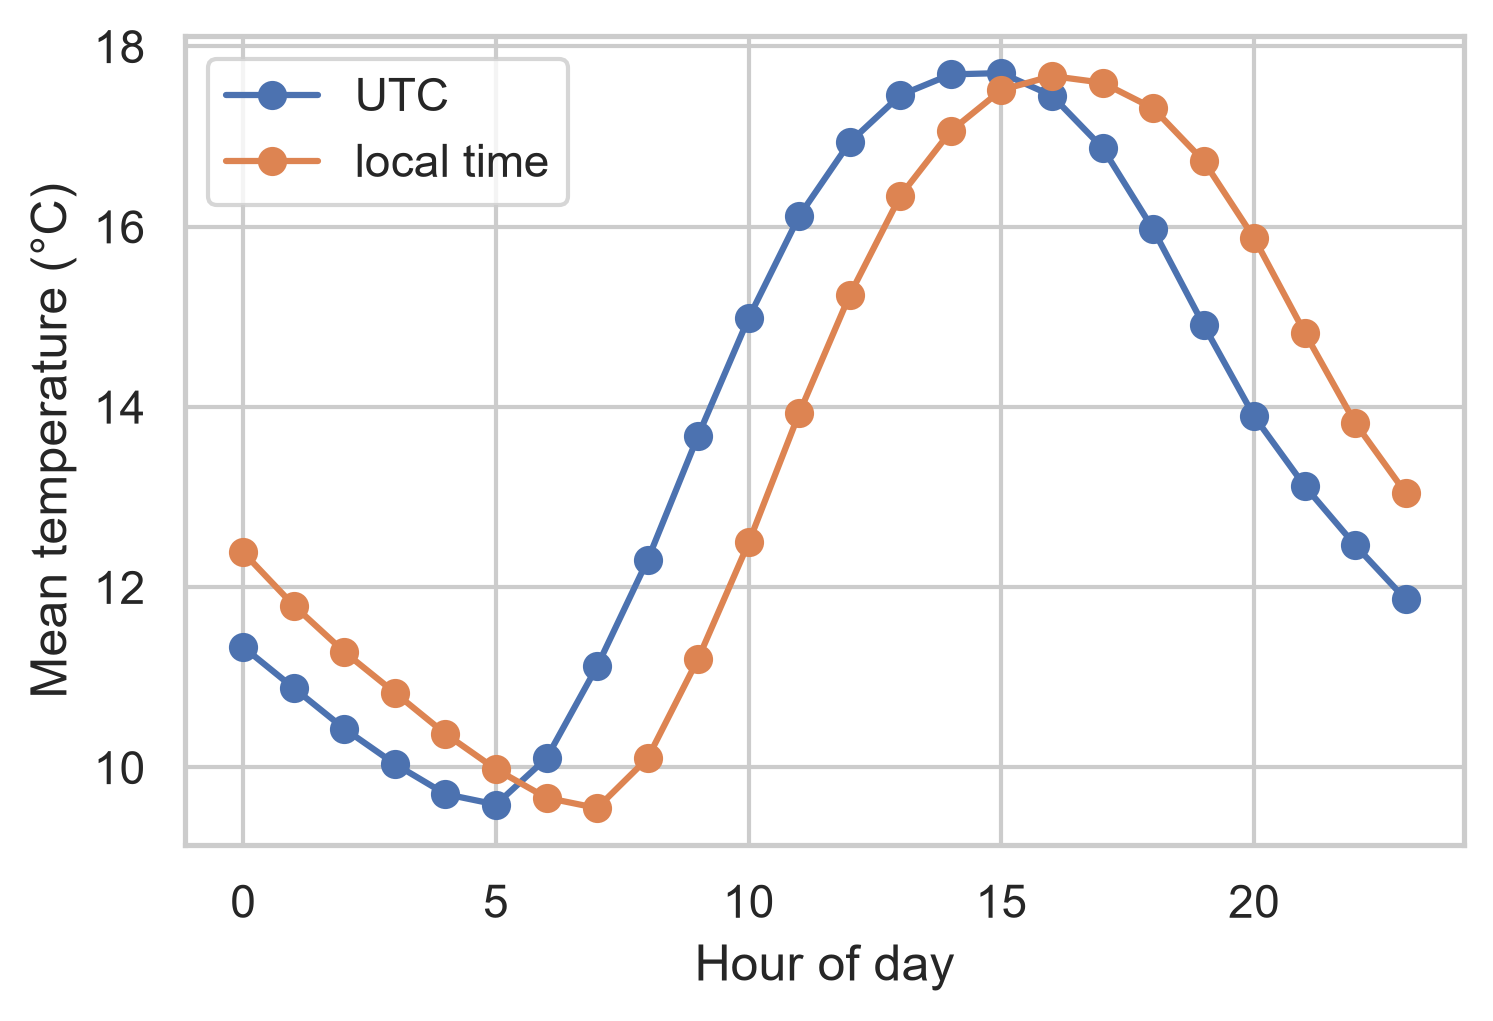
\includegraphics[keepaspectratio]{notebooks/02-eda_files/figure-pdf/cell-21-output-1.png}}

\begin{verbatim}
UTC           15
local time    16
dtype: int32
\end{verbatim}

The maximum typically occurs in the early or mid afternoon. In local
time the curve is shifted by one hour in winter and two hours in summer,
so the hour of the maximum changes accordingly. This is exactly the kind
of shift that causes errors when weather data are merged with production
data recorded in local time.

\end{tcolorbox}

\begin{tcolorbox}[enhanced jigsaw, colframe=quarto-callout-caution-color-frame, toprule=.15mm, rightrule=.15mm, title=\textcolor{quarto-callout-caution-color}{\faFire}\hspace{0.5em}{Solution to Exercise 8}, colbacktitle=quarto-callout-caution-color!10!white, left=2mm, titlerule=0mm, bottomtitle=1mm, toptitle=1mm, opacityback=0, bottomrule=.15mm, breakable, arc=.35mm, opacitybacktitle=0.6, colback=white, coltitle=black, leftrule=.75mm]

\begin{itemize}
\tightlist
\item
  \texttt{STATIONS\_ID}: categorical (nominal) -- a code, although
  stored as a number; constant within the file.
\item
  \texttt{MESS\_DATUM}: time stamp -- numeric (differences are
  durations); after conversion, the index of the time series.
\item
  \texttt{QN\_9}: categorical -- a code for the quality level of the
  record. Whether the levels are ordered must be looked up in the DWD
  documentation; computing a mean is meaningless either way.
\item
  \texttt{TT\_TU}: continuous (°C) -- the variable of interest for this
  question; there is no target, because nothing is predicted.
\item
  \texttt{RF\_TU}: continuous (\%) -- not needed for this question.
\item
  \texttt{eor}: not a variable at all -- a marker for ``end of record''
  in each line of the file.
\end{itemize}

\end{tcolorbox}

\chapter{Probability and Uncertainty}\label{probability-and-uncertainty}

No two measurements are identical, no two components have the same
lifetime, and every estimate computed from a sample would come out
slightly differently with another sample. Engineers deal with this
variability every day -- in tolerances, safety factors, reliability
targets and maintenance plans. Probability theory provides the language
to describe it, and statistics provides the tools to quantify how
certain our estimates are.

In this chapter we model the lifetimes of jet engines with a probability
distribution, derive reliability figures such as the B10 life, and
quantify the uncertainty of our estimates with confidence intervals --
computed both with a classical formula and with the bootstrap. Finally
we meet Bayes' theorem, which tells us how to update probabilities when
new information arrives.

\textbf{Scenario: the replacement interval}

You are the reliability engineer of an airline that operates a fleet of
turbofan engines of one type. The airworthiness authority requires a
maintenance programme in which, with 95 \% confidence, at most 10 \% of
the engines reach a critical degradation state before they are taken off
wing for overhaul. Your data: the complete run-to-failure histories of
100 engines of the same type. The fleet manager wants the interval as
long as possible -- every additional cycle on wing saves money.

\textbf{Your decision:} After how many flight cycles should engines be
overhauled preventively?

\textbf{Learning goals.} After this chapter you can

\begin{itemize}
\tightlist
\item
  describe random quantities with probability density, distribution
  function, expected value and variance,
\item
  choose suitable distributions for engineering data (normal, lognormal,
  Weibull, exponential),
\item
  fit a distribution to lifetime data by maximum likelihood and check
  the fit with a probability plot,
\item
  interpret the Weibull shape parameter in terms of failure behaviour
  and derive the B10 life,
\item
  compute and correctly interpret confidence intervals, analytically and
  with the bootstrap,
\item
  apply Bayes' theorem to diagnostic alarms and explain the base rate
  effect,
\item
  (extension) update prior knowledge with test data (beta--binomial
  model) and interpret a credible interval.
\end{itemize}

\textbf{Datasets in this chapter}

\begin{itemize}
\tightlist
\item
  \href{https://data.nasa.gov/dataset/cmapss-jet-engine-simulated-data}{NASA
  C-MAPSS turbofan degradation data}
\end{itemize}

\section{Random variables and
distributions}\label{random-variables-and-distributions}

\begin{tcolorbox}[enhanced jigsaw, colframe=quarto-callout-note-color-frame, toprule=.15mm, rightrule=.15mm, title=\textcolor{quarto-callout-note-color}{\faInfo}\hspace{0.5em}{Definition: Random variable, PDF and CDF}, colbacktitle=quarto-callout-note-color!10!white, left=2mm, titlerule=0mm, bottomtitle=1mm, toptitle=1mm, opacityback=0, bottomrule=.15mm, breakable, arc=.35mm, opacitybacktitle=0.6, colback=white, coltitle=black, leftrule=.75mm]

A \textbf{random variable} \(X\) assigns a number to the outcome of a
random experiment, e.g.~the lifetime of a component. For a continuous
random variable,

\begin{itemize}
\tightlist
\item
  the \textbf{cumulative distribution function (CDF)}
  \(F(x) = P(X \le x)\) gives the probability of a value up to \(x\),
\item
  the \textbf{probability density function (PDF)} \(f(x) = F'(x)\)
  describes how probability is distributed;
  \(P(a < X \le b) = \int_a^b f(x)\,dx\).
\end{itemize}

The \textbf{expected value} \(E[X] = \int x\,f(x)\,dx\) is the long-run
average, the \textbf{variance} \(\text{Var}(X) = E[(X - E[X])^2]\)
measures the spread.

\end{tcolorbox}

In reliability engineering, \(F(t)\) is the probability that a component
has failed by time \(t\), and the \textbf{reliability} (survival
function) is \(R(t) = 1 - F(t)\).

Choosing a distribution is a modelling decision, guided by physics and
by the data:

\begin{longtable}[]{@{}
  >{\raggedright\arraybackslash}p{(\linewidth - 6\tabcolsep) * \real{0.2500}}
  >{\raggedright\arraybackslash}p{(\linewidth - 6\tabcolsep) * \real{0.2500}}
  >{\raggedright\arraybackslash}p{(\linewidth - 6\tabcolsep) * \real{0.2500}}
  >{\raggedright\arraybackslash}p{(\linewidth - 6\tabcolsep) * \real{0.2500}}@{}}
\toprule\noalign{}
\begin{minipage}[b]{\linewidth}\raggedright
Distribution
\end{minipage} & \begin{minipage}[b]{\linewidth}\raggedright
Parameters
\end{minipage} & \begin{minipage}[b]{\linewidth}\raggedright
Typical use
\end{minipage} & \begin{minipage}[b]{\linewidth}\raggedright
Physical reasoning
\end{minipage} \\
\midrule\noalign{}
\endhead
\bottomrule\noalign{}
\endlastfoot
Normal & \(\mu\), \(\sigma\) & measurement errors, machined dimensions &
sum of many small independent effects \\
Lognormal & \(\mu\), \(\sigma\) of \(\ln X\) & fatigue life, particle
sizes, repair times & product of many small independent effects \\
Weibull & shape \(\beta\), scale \(\eta\) & lifetimes, strength of
brittle materials & ``weakest link'': the first of many flaws fails \\
Exponential & rate \(\lambda\) & random failures, times between events &
constant failure rate, no memory \\
Poisson & rate \(\lambda\) & number of defects per unit or per time &
rare independent events \\
\end{longtable}

The prominence of the normal distribution is explained by one of the
most important results of probability theory:

\begin{tcolorbox}[enhanced jigsaw, colframe=quarto-callout-important-color-frame, toprule=.15mm, rightrule=.15mm, title=\textcolor{quarto-callout-important-color}{\faExclamation}\hspace{0.5em}{Theorem: Central limit theorem}, colbacktitle=quarto-callout-important-color!10!white, left=2mm, titlerule=0mm, bottomtitle=1mm, toptitle=1mm, opacityback=0, bottomrule=.15mm, breakable, arc=.35mm, opacitybacktitle=0.6, colback=white, coltitle=black, leftrule=.75mm]

Let \(X_1, \dots, X_n\) be independent random variables with the same
distribution, mean \(\mu\) and finite variance \(\sigma^2\). Then the
distribution of the sample mean \(\bar X_n\) approaches a normal
distribution with mean \(\mu\) and standard deviation
\(\sigma/\sqrt{n}\) as \(n\) grows -- \textbf{whatever the distribution
of the \(X_i\)}.

\end{tcolorbox}

Two consequences matter for engineers: quantities that arise as sums of
many small effects are approximately normal, and the uncertainty of a
mean decreases with \(1/\sqrt{n}\) -- four times as many measurements
halve the uncertainty.

\section{The Weibull distribution for
lifetimes}\label{the-weibull-distribution-for-lifetimes}

The two-parameter Weibull distribution has the CDF and the
\textbf{hazard rate} (instantaneous failure rate of the survivors)

\[F(t) = 1 - \exp\left[-\left(\frac{t}{\eta}\right)^{\beta}\right], \qquad h(t) = \frac{f(t)}{R(t)} = \frac{\beta}{\eta}\left(\frac{t}{\eta}\right)^{\beta - 1}.\]

The scale parameter \(\eta\) is the \textbf{characteristic life}: by
\(t = \eta\), 63.2 \% of all units have failed, regardless of \(\beta\).
The shape parameter \(\beta\) determines how the failure rate changes
over time:

\begin{tcolorbox}[enhanced jigsaw, colframe=quarto-callout-important-color-frame, toprule=.15mm, rightrule=.15mm, title=\textcolor{quarto-callout-important-color}{\faExclamation}\hspace{0.5em}{Interpretation of the Weibull shape parameter}, colbacktitle=quarto-callout-important-color!10!white, left=2mm, titlerule=0mm, bottomtitle=1mm, toptitle=1mm, opacityback=0, bottomrule=.15mm, breakable, arc=.35mm, opacitybacktitle=0.6, colback=white, coltitle=black, leftrule=.75mm]

\begin{itemize}
\tightlist
\item
  \(\beta < 1\): decreasing failure rate -- \textbf{early failures}
  (manufacturing defects, infant mortality).
\item
  \(\beta = 1\): constant failure rate -- \textbf{random failures}; the
  Weibull becomes the exponential distribution.
\item
  \(\beta > 1\): increasing failure rate -- \textbf{wear-out} (fatigue,
  corrosion, abrasion). \(\beta \approx 3.5\) gives a nearly symmetric
  distribution.
\end{itemize}

Together, the three regimes form the well-known \emph{bathtub curve} of
a product's life.

\end{tcolorbox}

\begin{figure}[H]

\centering{

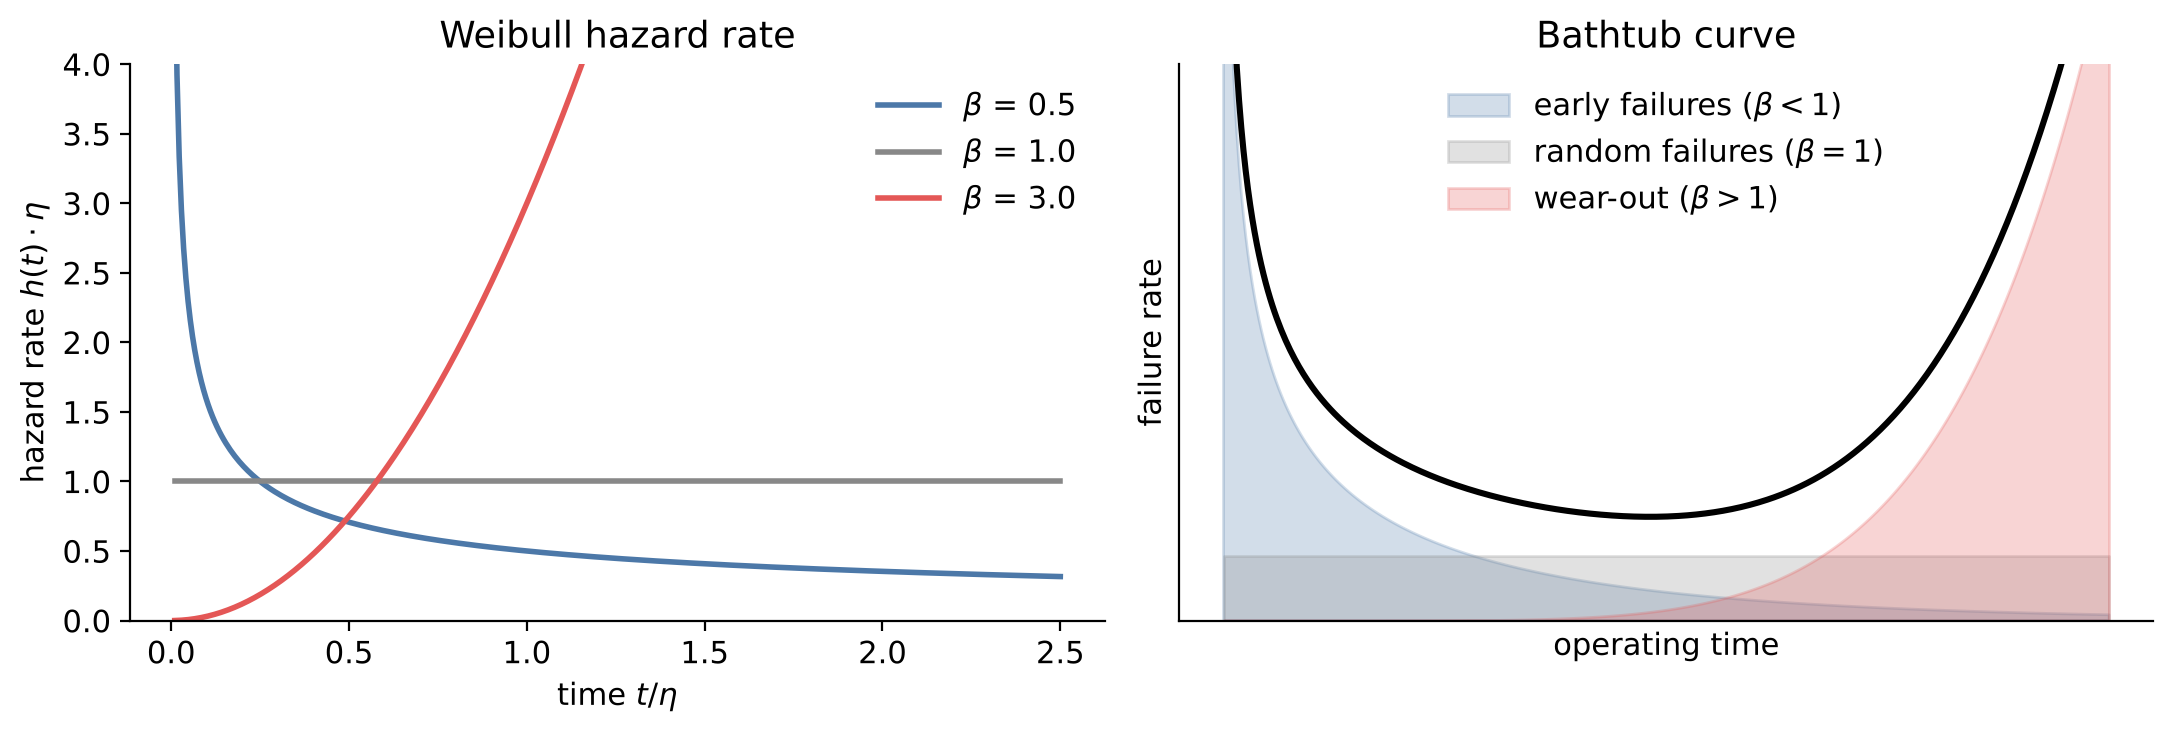
\includegraphics[width=1\linewidth,height=\textheight,keepaspectratio]{notebooks/images/bathtub.png}

}

\caption{\label{fig-bathtub}Left: Weibull hazard rate for different
shape parameters. Right: the bathtub curve of a product's life as the
superposition of early failures, random failures and wear-out.}

\end{figure}%

The shape parameter has direct consequences for maintenance: preventive
replacement only makes sense if the failure rate increases
(\(\beta > 1\)). With \(\beta \le 1\), a new part is not more reliable
than an old one, and replacing it early wastes money.

A frequently used reliability figure is the \textbf{B10 life}: the time
by which 10 \% of the units have failed, i.e.~\(F(B_{10}) = 0.1\).
Solving the Weibull CDF gives

\[B_{10} = \eta\,\left(-\ln 0.9\right)^{1/\beta}.\]

\subsection{Estimating parameters: maximum
likelihood}\label{estimating-parameters-maximum-likelihood}

\begin{tcolorbox}[enhanced jigsaw, colframe=quarto-callout-note-color-frame, toprule=.15mm, rightrule=.15mm, title=\textcolor{quarto-callout-note-color}{\faInfo}\hspace{0.5em}{Definition: Maximum likelihood estimation (MLE)}, colbacktitle=quarto-callout-note-color!10!white, left=2mm, titlerule=0mm, bottomtitle=1mm, toptitle=1mm, opacityback=0, bottomrule=.15mm, breakable, arc=.35mm, opacitybacktitle=0.6, colback=white, coltitle=black, leftrule=.75mm]

Given independent observations \(x_1, \dots, x_n\) and a model with
density \(f(x;\theta)\), the \textbf{likelihood}
\(L(\theta) = \prod_i f(x_i;\theta)\) measures how plausible the data
are for a parameter value \(\theta\). The maximum likelihood estimate
\(\hat\theta\) maximises \(L\), in practice its logarithm
\(\ell(\theta) = \sum_i \ln f(x_i;\theta)\).

\end{tcolorbox}

For the normal distribution, MLE leads to the familiar mean and (biased)
standard deviation. For the Weibull distribution, there is no
closed-form solution; \texttt{scipy.stats.weibull\_min.fit} maximises
the likelihood numerically.

To check whether the fitted distribution describes the data, we use a
\textbf{probability plot} (Q--Q plot): the sorted data are plotted
against the corresponding quantiles of the fitted distribution. If the
model fits, the points lie on a straight line. Systematic curvature at
the ends reveals a wrong tail behaviour -- exactly where reliability
questions are decided.

\begin{Shaded}
\begin{Highlighting}[]
\CommentTok{\# Setup: works locally and in Google Colab}
\ImportTok{import}\NormalTok{ numpy }\ImportTok{as}\NormalTok{ np}
\ImportTok{import}\NormalTok{ pandas }\ImportTok{as}\NormalTok{ pd}
\ImportTok{import}\NormalTok{ matplotlib.pyplot }\ImportTok{as}\NormalTok{ plt}
\ImportTok{import}\NormalTok{ seaborn }\ImportTok{as}\NormalTok{ sns}
\ImportTok{from}\NormalTok{ scipy }\ImportTok{import}\NormalTok{ stats}

\NormalTok{sns.set\_theme(style}\OperatorTok{=}\StringTok{"whitegrid"}\NormalTok{)}
\end{Highlighting}
\end{Shaded}

\section{Live coding: lifetimes of turbofan
engines}\label{live-coding-lifetimes-of-turbofan-engines}

C-MAPSS (\emph{Commercial Modular Aero-Propulsion System Simulation}) is
a NASA simulation of a large turbofan engine. The dataset contains
run-to-failure trajectories of a fleet of engines with different initial
wear and manufacturing variation. In the training file
\texttt{train\_FD001.txt}, every one of the 100 engines runs until
failure, so the last recorded cycle of each engine is its lifetime (in
flight cycles). We will use the sensor data of the same file in Chapter
12.

\textbf{Data access.} The cell below downloads \texttt{CMAPSSData.zip}
(about 12 MB) from the NASA Open Data Portal once and extracts it into
the folder \texttt{data/CMAPSSData/}.

\begin{Shaded}
\begin{Highlighting}[]
\ImportTok{from}\NormalTok{ pathlib }\ImportTok{import}\NormalTok{ Path}
\ImportTok{import}\NormalTok{ zipfile, io, requests}

\KeywordTok{def}\NormalTok{ cmapss\_dir(root}\OperatorTok{=}\NormalTok{Path(}\StringTok{"data"}\NormalTok{)):}
    \CommentTok{"""Download and extract the NASA C{-}MAPSS data once; return the folder with train\_FD001.txt."""}
\NormalTok{    root.mkdir(exist\_ok}\OperatorTok{=}\VariableTok{True}\NormalTok{)}
\NormalTok{    target }\OperatorTok{=}\NormalTok{ root }\OperatorTok{/} \StringTok{"CMAPSSData"}
    \ControlFlowTok{if} \KeywordTok{not} \BuiltInTok{any}\NormalTok{(target.rglob(}\StringTok{"train\_FD001.txt"}\NormalTok{)):}
\NormalTok{        zip\_path }\OperatorTok{=}\NormalTok{ root }\OperatorTok{/} \StringTok{"CMAPSSData.zip"}
        \ControlFlowTok{if} \KeywordTok{not}\NormalTok{ zip\_path.exists():}
\NormalTok{            r }\OperatorTok{=}\NormalTok{ requests.get(}\StringTok{"https://data.nasa.gov/docs/legacy/CMAPSSData.zip"}\NormalTok{, timeout}\OperatorTok{=}\DecValTok{300}\NormalTok{)}
\NormalTok{            r.raise\_for\_status()}
\NormalTok{            zip\_path.write\_bytes(r.content)}
        \ControlFlowTok{with}\NormalTok{ zipfile.ZipFile(zip\_path) }\ImportTok{as}\NormalTok{ z:}
\NormalTok{            z.extractall(target)}
        \ControlFlowTok{for}\NormalTok{ inner }\KeywordTok{in} \BuiltInTok{list}\NormalTok{(target.rglob(}\StringTok{"*.zip"}\NormalTok{)):          }\CommentTok{\# some versions contain a nested zip}
\NormalTok{            zipfile.ZipFile(inner).extractall(inner.parent)}
    \ControlFlowTok{return} \BuiltInTok{next}\NormalTok{(target.rglob(}\StringTok{"train\_FD001.txt"}\NormalTok{)).parent}

\NormalTok{CMAPSS }\OperatorTok{=}\NormalTok{ cmapss\_dir()}
\NormalTok{cols }\OperatorTok{=}\NormalTok{ [}\StringTok{"unit"}\NormalTok{, }\StringTok{"cycle"}\NormalTok{, }\StringTok{"op1"}\NormalTok{, }\StringTok{"op2"}\NormalTok{, }\StringTok{"op3"}\NormalTok{] }\OperatorTok{+}\NormalTok{ [}\SpecialStringTok{f"s}\SpecialCharTok{\{}\NormalTok{i}\SpecialCharTok{\}}\SpecialStringTok{"} \ControlFlowTok{for}\NormalTok{ i }\KeywordTok{in} \BuiltInTok{range}\NormalTok{(}\DecValTok{1}\NormalTok{, }\DecValTok{22}\NormalTok{)]}
\NormalTok{train }\OperatorTok{=}\NormalTok{ pd.read\_csv(CMAPSS }\OperatorTok{/} \StringTok{"train\_FD001.txt"}\NormalTok{, sep}\OperatorTok{=}\VerbatimStringTok{r"\textbackslash{}s+"}\NormalTok{, header}\OperatorTok{=}\VariableTok{None}\NormalTok{, names}\OperatorTok{=}\NormalTok{cols)}
\NormalTok{lifetimes }\OperatorTok{=}\NormalTok{ train.groupby(}\StringTok{"unit"}\NormalTok{)[}\StringTok{"cycle"}\NormalTok{].}\BuiltInTok{max}\NormalTok{()}
\NormalTok{lifetimes.describe().}\BuiltInTok{round}\NormalTok{(}\DecValTok{1}\NormalTok{)}
\end{Highlighting}
\end{Shaded}

\begin{verbatim}
count    100.0
mean     206.3
std       46.3
min      128.0
25%      177.0
50%      199.0
75%      229.2
max      362.0
Name: cycle, dtype: float64
\end{verbatim}

\begin{Shaded}
\begin{Highlighting}[]
\NormalTok{beta, loc, eta }\OperatorTok{=}\NormalTok{ stats.weibull\_min.fit(lifetimes, floc}\OperatorTok{=}\DecValTok{0}\NormalTok{)}
\BuiltInTok{print}\NormalTok{(}\SpecialStringTok{f"Weibull fit: shape beta = }\SpecialCharTok{\{}\NormalTok{beta}\SpecialCharTok{:.2f\}}\SpecialStringTok{, scale eta = }\SpecialCharTok{\{}\NormalTok{eta}\SpecialCharTok{:.1f\}}\SpecialStringTok{ cycles"}\NormalTok{)}

\NormalTok{fig, axes }\OperatorTok{=}\NormalTok{ plt.subplots(}\DecValTok{1}\NormalTok{, }\DecValTok{2}\NormalTok{, figsize}\OperatorTok{=}\NormalTok{(}\DecValTok{11}\NormalTok{, }\DecValTok{4}\NormalTok{))}
\NormalTok{t }\OperatorTok{=}\NormalTok{ np.linspace(}\DecValTok{0}\NormalTok{, lifetimes.}\BuiltInTok{max}\NormalTok{() }\OperatorTok{*} \FloatTok{1.1}\NormalTok{, }\DecValTok{300}\NormalTok{)}
\NormalTok{axes[}\DecValTok{0}\NormalTok{].hist(lifetimes, bins}\OperatorTok{=}\DecValTok{15}\NormalTok{, density}\OperatorTok{=}\VariableTok{True}\NormalTok{, alpha}\OperatorTok{=}\FloatTok{0.6}\NormalTok{, label}\OperatorTok{=}\StringTok{"data"}\NormalTok{)}
\NormalTok{axes[}\DecValTok{0}\NormalTok{].plot(t, stats.weibull\_min.pdf(t, beta, scale}\OperatorTok{=}\NormalTok{eta), label}\OperatorTok{=}\StringTok{"Weibull fit"}\NormalTok{)}
\NormalTok{axes[}\DecValTok{0}\NormalTok{].}\BuiltInTok{set}\NormalTok{(xlabel}\OperatorTok{=}\StringTok{"Lifetime (cycles)"}\NormalTok{, ylabel}\OperatorTok{=}\StringTok{"Density"}\NormalTok{)}\OperatorTok{;}\NormalTok{ axes[}\DecValTok{0}\NormalTok{].legend()}
\NormalTok{stats.probplot(lifetimes, dist}\OperatorTok{=}\NormalTok{stats.weibull\_min, sparams}\OperatorTok{=}\NormalTok{(beta, }\DecValTok{0}\NormalTok{, eta), plot}\OperatorTok{=}\NormalTok{axes[}\DecValTok{1}\NormalTok{])}
\NormalTok{axes[}\DecValTok{1}\NormalTok{].set\_title(}\StringTok{"Probability plot (Weibull)"}\NormalTok{)}
\NormalTok{plt.show()}
\end{Highlighting}
\end{Shaded}

\begin{verbatim}
Weibull fit: shape beta = 4.41, scale eta = 225.0 cycles
\end{verbatim}

\pandocbounded{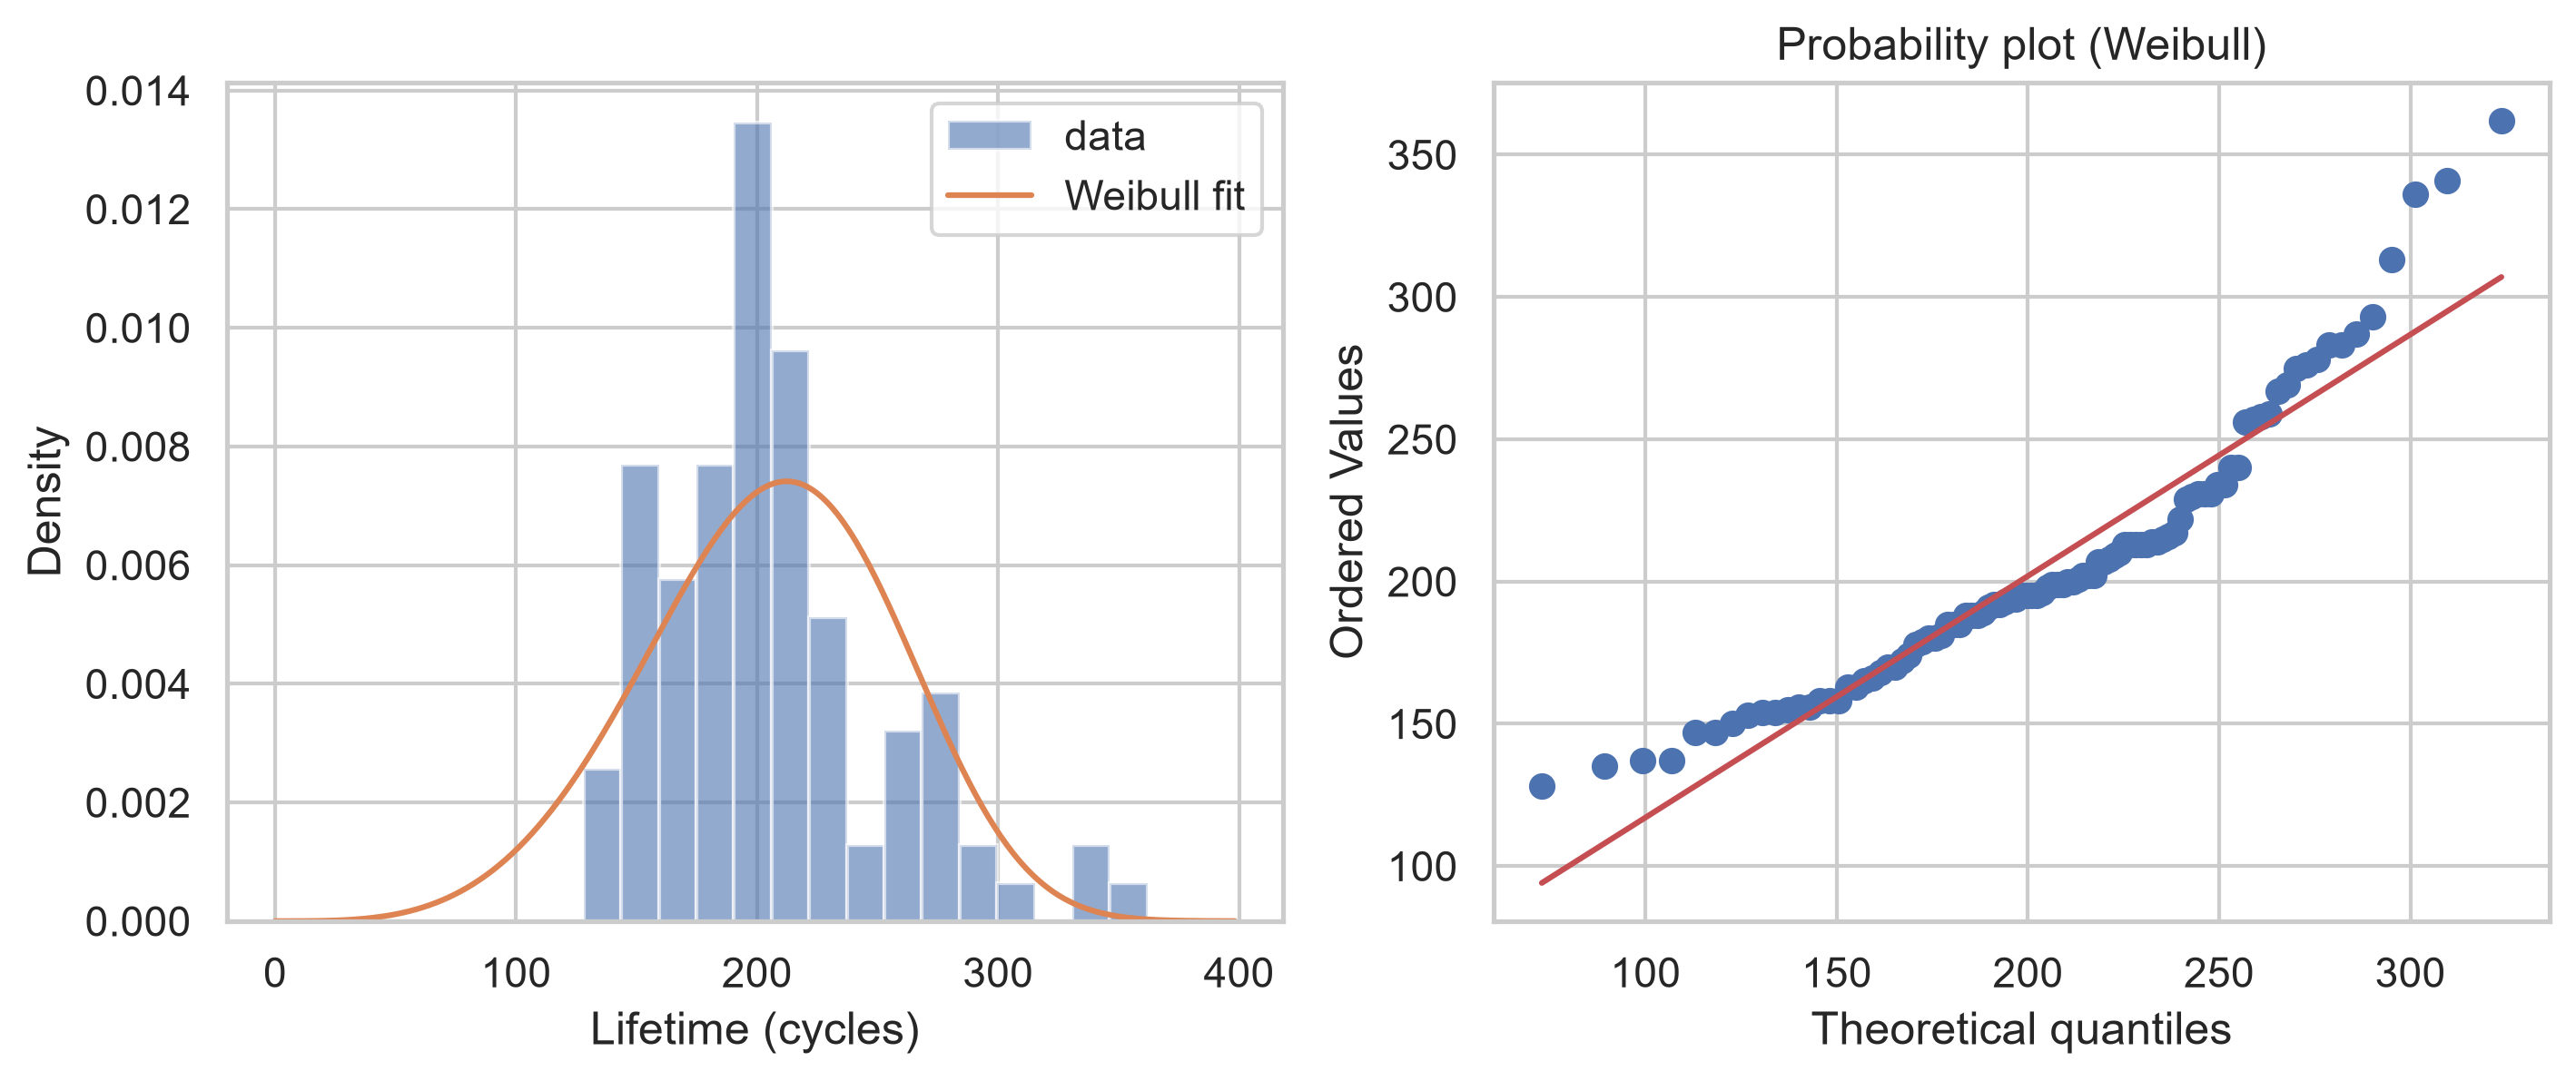
\includegraphics[keepaspectratio]{notebooks/03-uncertainty_files/figure-pdf/cell-4-output-2.png}}

\textbf{Discussion.} We fixed the location parameter at zero
(\texttt{floc=0}), i.e.~we use the two-parameter Weibull distribution.
The estimated shape parameter is clearly larger than 1 -- the engines
show \textbf{wear-out behaviour}, as expected for a degradation
simulation. The probability plot tells us whether the Weibull model is
adequate over the whole range; pay particular attention to the lower
tail, which determines the B10 life.

Note that no engine fails very early: the shortest lifetime is well
above zero. A three-parameter Weibull distribution with a
\emph{failure-free time} (location parameter \(t_0 > 0\)) could describe
this better -- a question for Exercise 1.

\begin{Shaded}
\begin{Highlighting}[]
\NormalTok{b10 }\OperatorTok{=}\NormalTok{ stats.weibull\_min.ppf(}\FloatTok{0.10}\NormalTok{, beta, scale}\OperatorTok{=}\NormalTok{eta)}
\BuiltInTok{print}\NormalTok{(}\SpecialStringTok{f"B10 life from the fit:    }\SpecialCharTok{\{}\NormalTok{b10}\SpecialCharTok{:.0f\}}\SpecialStringTok{ cycles"}\NormalTok{)}
\BuiltInTok{print}\NormalTok{(}\SpecialStringTok{f"B10 from the formula:     }\SpecialCharTok{\{}\NormalTok{eta }\OperatorTok{*}\NormalTok{ (}\OperatorTok{{-}}\NormalTok{np.log(}\FloatTok{0.9}\NormalTok{)) }\OperatorTok{**}\NormalTok{ (}\DecValTok{1} \OperatorTok{/}\NormalTok{ beta)}\SpecialCharTok{:.0f\}}\SpecialStringTok{ cycles"}\NormalTok{)}
\BuiltInTok{print}\NormalTok{(}\SpecialStringTok{f"Empirical 10 \% quantile:  }\SpecialCharTok{\{}\NormalTok{lifetimes}\SpecialCharTok{.}\NormalTok{quantile(}\FloatTok{0.10}\NormalTok{)}\SpecialCharTok{:.0f\}}\SpecialStringTok{ cycles"}\NormalTok{)}
\end{Highlighting}
\end{Shaded}

\begin{verbatim}
B10 life from the fit:    135 cycles
B10 from the formula:     135 cycles
Empirical 10 % quantile:  155 cycles
\end{verbatim}

\section{Confidence intervals}\label{confidence-intervals}

The mean lifetime we computed is an \textbf{estimate} from 100 engines.
Another fleet of 100 engines would give a somewhat different value. A
confidence interval quantifies this sampling uncertainty.

\begin{tcolorbox}[enhanced jigsaw, colframe=quarto-callout-note-color-frame, toprule=.15mm, rightrule=.15mm, title=\textcolor{quarto-callout-note-color}{\faInfo}\hspace{0.5em}{Definition: Confidence interval}, colbacktitle=quarto-callout-note-color!10!white, left=2mm, titlerule=0mm, bottomtitle=1mm, toptitle=1mm, opacityback=0, bottomrule=.15mm, breakable, arc=.35mm, opacitybacktitle=0.6, colback=white, coltitle=black, leftrule=.75mm]

A 95 \% \textbf{confidence interval} is computed from the data by a
procedure that, if the experiment were repeated many times, would
contain the true parameter in 95 \% of the repetitions.

For the mean of approximately normal data (or large \(n\) by the central
limit theorem): \[\bar x \pm t_{n-1,\,0.975}\,\frac{s}{\sqrt n},\] where
\(t_{n-1,\,0.975}\) is the 97.5 \% quantile of the t-distribution with
\(n-1\) degrees of freedom (\(\approx 1.98\) for \(n = 100\)).

\end{tcolorbox}

\begin{figure}[H]

\centering{

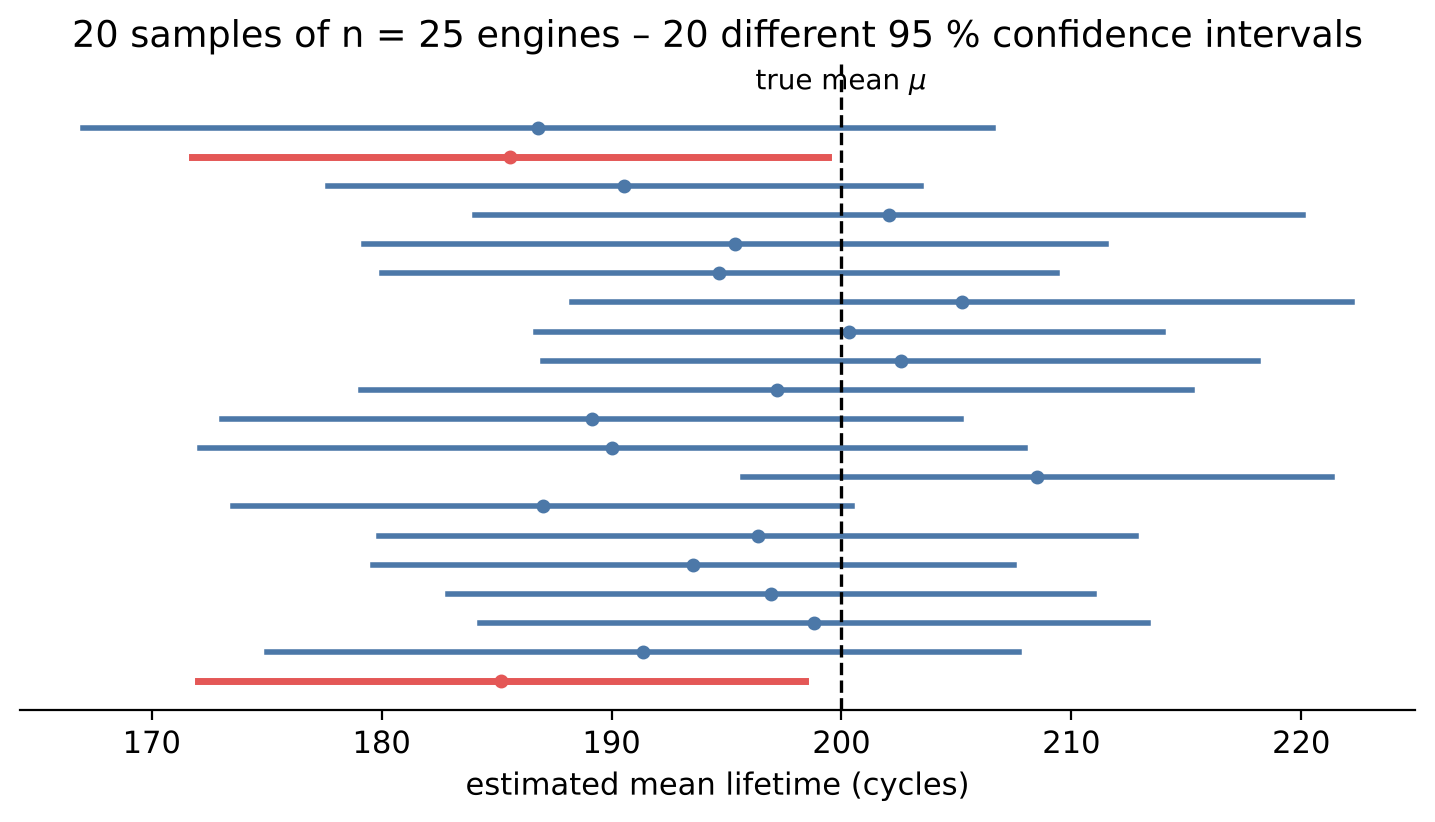
\includegraphics[width=0.9\linewidth,height=\textheight,keepaspectratio]{notebooks/images/ci-coverage.png}

}

\caption{\label{fig-cicoverage}Twenty repetitions of the same
experiment, each with its own 95 \% confidence interval for the mean. On
average, 19 of 20 intervals contain the true mean; here two miss it
(red). For a single computed interval we never know whether it is one of
the lucky ones.}

\end{figure}%

\begin{tcolorbox}[enhanced jigsaw, colframe=quarto-callout-warning-color-frame, toprule=.15mm, rightrule=.15mm, title=\textcolor{quarto-callout-warning-color}{\faExclamationTriangle}\hspace{0.5em}{Pitfall: what a confidence interval does \emph{not} say}, colbacktitle=quarto-callout-warning-color!10!white, left=2mm, titlerule=0mm, bottomtitle=1mm, toptitle=1mm, opacityback=0, bottomrule=.15mm, breakable, arc=.35mm, opacitybacktitle=0.6, colback=white, coltitle=black, leftrule=.75mm]

A computed interval, say {[}195, 215{]} cycles, does \textbf{not}
contain the true mean ``with 95 \% probability'' -- in the classical
view, the true mean is fixed and either inside or not. The 95 \% refers
to the reliability of the method. Also, a confidence interval for the
\emph{mean} says nothing about the spread of \emph{individual}
lifetimes: most single engines lie far outside it.

\end{tcolorbox}

For many quantities -- the B10 life, a median, a ratio -- there is no
simple formula for the interval. The bootstrap solves this by
simulation:

\begin{tcolorbox}[enhanced jigsaw, colframe=quarto-callout-note-color-frame, toprule=.15mm, rightrule=.15mm, title=\textcolor{quarto-callout-note-color}{\faInfo}\hspace{0.5em}{Definition: Bootstrap}, colbacktitle=quarto-callout-note-color!10!white, left=2mm, titlerule=0mm, bottomtitle=1mm, toptitle=1mm, opacityback=0, bottomrule=.15mm, breakable, arc=.35mm, opacitybacktitle=0.6, colback=white, coltitle=black, leftrule=.75mm]

Draw \(B\) (e.g.~10,000) samples of size \(n\) \textbf{with replacement}
from the observed data and compute the statistic of interest for each.
The distribution of these bootstrap replicates approximates the sampling
distribution of the statistic; its 2.5 \% and 97.5 \% quantiles give an
approximate 95 \% confidence interval (percentile method; SciPy uses the
refined BCa method by default).

\end{tcolorbox}

\begin{Shaded}
\begin{Highlighting}[]
\NormalTok{ci\_t }\OperatorTok{=}\NormalTok{ stats.t.interval(}\FloatTok{0.95}\NormalTok{, df}\OperatorTok{=}\BuiltInTok{len}\NormalTok{(lifetimes) }\OperatorTok{{-}} \DecValTok{1}\NormalTok{,}
\NormalTok{                        loc}\OperatorTok{=}\NormalTok{lifetimes.mean(), scale}\OperatorTok{=}\NormalTok{stats.sem(lifetimes))}
\NormalTok{boot }\OperatorTok{=}\NormalTok{ stats.bootstrap((lifetimes.values,), np.mean, confidence\_level}\OperatorTok{=}\FloatTok{0.95}\NormalTok{,}
\NormalTok{                       random\_state}\OperatorTok{=}\DecValTok{0}\NormalTok{)}
\BuiltInTok{print}\NormalTok{(}\SpecialStringTok{f"Mean lifetime: }\SpecialCharTok{\{}\NormalTok{lifetimes}\SpecialCharTok{.}\NormalTok{mean()}\SpecialCharTok{:.1f\}}\SpecialStringTok{ cycles"}\NormalTok{)}
\BuiltInTok{print}\NormalTok{(}\StringTok{"t{-}interval:        "}\NormalTok{, np.}\BuiltInTok{round}\NormalTok{(ci\_t, }\DecValTok{1}\NormalTok{))}
\BuiltInTok{print}\NormalTok{(}\StringTok{"bootstrap interval:"}\NormalTok{, np.}\BuiltInTok{round}\NormalTok{(boot.confidence\_interval, }\DecValTok{1}\NormalTok{))}
\end{Highlighting}
\end{Shaded}

\begin{verbatim}
Mean lifetime: 206.3 cycles
t-interval:         [197.1 215.5]
bootstrap interval: [197.9 215.8]
\end{verbatim}

\textbf{Discussion.} For the mean of 100 observations both methods give
almost the same interval -- the central limit theorem makes the
t-interval reliable here. The bootstrap becomes valuable for statistics
without a known formula (Exercise 2) and for small or strongly skewed
samples.

\section{Back to the decision}\label{back-to-the-decision-2}

The requirement ``at most 10 \% failures with 95 \% confidence'' has two
parts. The 10 \% defines the B10 life. The 95 \% confidence means that
we must not use the point estimate of B10 but a value that is, with 95
\% confidence, \emph{below} the true B10 -- the lower bound of a
one-sided 95 \% confidence interval, which we obtain with the bootstrap.
And preventive overhaul only makes sense if the failure rate increases
with age, i.e.~\(\beta > 1\).

\begin{Shaded}
\begin{Highlighting}[]
\KeywordTok{def}\NormalTok{ b10\_of(x):}
\NormalTok{    c, \_, scale }\OperatorTok{=}\NormalTok{ stats.weibull\_min.fit(x, floc}\OperatorTok{=}\DecValTok{0}\NormalTok{)}
    \ControlFlowTok{return}\NormalTok{ stats.weibull\_min.ppf(}\FloatTok{0.10}\NormalTok{, c, scale}\OperatorTok{=}\NormalTok{scale)}

\NormalTok{boot\_b10 }\OperatorTok{=}\NormalTok{ stats.bootstrap((lifetimes.values,), b10\_of, n\_resamples}\OperatorTok{=}\DecValTok{1000}\NormalTok{, confidence\_level}\OperatorTok{=}\FloatTok{0.90}\NormalTok{,}
\NormalTok{                           method}\OperatorTok{=}\StringTok{"percentile"}\NormalTok{, random\_state}\OperatorTok{=}\DecValTok{1}\NormalTok{)}
\NormalTok{b10\_lower }\OperatorTok{=}\NormalTok{ boot\_b10.confidence\_interval.low      }\CommentTok{\# lower end of a 90 \% two{-}sided = 95 \% one{-}sided bound}
\BuiltInTok{print}\NormalTok{(}\SpecialStringTok{f"Weibull shape beta = }\SpecialCharTok{\{}\NormalTok{beta}\SpecialCharTok{:.2f\}}\SpecialStringTok{  {-}\textgreater{}  }\SpecialCharTok{\{}\StringTok{\textquotesingle{}wear{-}out: preventive overhaul is sensible\textquotesingle{}} \ControlFlowTok{if}\NormalTok{ beta }\OperatorTok{\textgreater{}} \DecValTok{1} \ControlFlowTok{else} \StringTok{\textquotesingle{}no wear{-}out: preventive overhaul does not help\textquotesingle{}}\SpecialCharTok{\}}\SpecialStringTok{"}\NormalTok{)}
\BuiltInTok{print}\NormalTok{(}\SpecialStringTok{f"B10 point estimate: }\SpecialCharTok{\{}\NormalTok{b10}\SpecialCharTok{:.0f\}}\SpecialStringTok{ cycles, 95 \% lower confidence bound: }\SpecialCharTok{\{}\NormalTok{b10\_lower}\SpecialCharTok{:.0f\}}\SpecialStringTok{ cycles"}\NormalTok{)}
\BuiltInTok{print}\NormalTok{(}\SpecialStringTok{f"Decision: overhaul after }\SpecialCharTok{\{}\BuiltInTok{int}\NormalTok{(np.floor(b10\_lower))}\SpecialCharTok{\}}\SpecialStringTok{ flight cycles at the latest."}\NormalTok{)}
\end{Highlighting}
\end{Shaded}

\begin{verbatim}
Weibull shape beta = 4.41  ->  wear-out: preventive overhaul is sensible
B10 point estimate: 135 cycles, 95 % lower confidence bound: 128 cycles
Decision: overhaul after 128 flight cycles at the latest.
\end{verbatim}

The difference between the point estimate and the lower bound is the
price of having data from only 100 engines -- more data would allow a
longer interval. In the real world, the decision would also consider
that C-MAPSS is a \emph{simulation}: before an interval is approved, the
model would have to be validated against field data of real engines.

\section{Bayes' theorem: how much should we trust an
alarm?}\label{bayes-theorem-how-much-should-we-trust-an-alarm}

So far we have treated probabilities as long-run frequencies.
\textbf{Conditional probabilities} describe how the probability of an
event changes when we know that another event has occurred.

\begin{tcolorbox}[enhanced jigsaw, colframe=quarto-callout-important-color-frame, toprule=.15mm, rightrule=.15mm, title=\textcolor{quarto-callout-important-color}{\faExclamation}\hspace{0.5em}{Theorem: Bayes' theorem}, colbacktitle=quarto-callout-important-color!10!white, left=2mm, titlerule=0mm, bottomtitle=1mm, toptitle=1mm, opacityback=0, bottomrule=.15mm, breakable, arc=.35mm, opacitybacktitle=0.6, colback=white, coltitle=black, leftrule=.75mm]

For events \(F\) and \(A\) with \(P(A) > 0\):
\[P(F \mid A) = \frac{P(A \mid F)\,P(F)}{P(A)} = \frac{P(A \mid F)\,P(F)}{P(A \mid F)\,P(F) + P(A \mid \bar F)\,P(\bar F)}.\]
\(P(F)\) is the \textbf{prior} probability, \(P(F \mid A)\) the
\textbf{posterior} probability after observing \(A\).

\end{tcolorbox}

Example: a condition monitoring system detects a bearing fault \(F\)
with probability \(P(A \mid F) = 0.95\) (\emph{sensitivity}) and raises
a false alarm on a healthy bearing with probability
\(P(A \mid \bar F) = 0.05\). Only 1 \% of the monitored bearings are
actually damaged. If the system raises an alarm \(A\), how likely is a
real fault?

\[P(F \mid A) = \frac{0.95 \cdot 0.01}{0.95 \cdot 0.01 + 0.05 \cdot 0.99} \approx 0.16\]

Five out of six alarms are false -- not because the system is bad, but
because faults are rare.

\begin{tcolorbox}[enhanced jigsaw, colframe=quarto-callout-warning-color-frame, toprule=.15mm, rightrule=.15mm, title=\textcolor{quarto-callout-warning-color}{\faExclamationTriangle}\hspace{0.5em}{Pitfall: base rate neglect}, colbacktitle=quarto-callout-warning-color!10!white, left=2mm, titlerule=0mm, bottomtitle=1mm, toptitle=1mm, opacityback=0, bottomrule=.15mm, breakable, arc=.35mm, opacitybacktitle=0.6, colback=white, coltitle=black, leftrule=.75mm]

Intuition tends to confuse \(P(A \mid F)\) (``the system detects 95 \%
of all faults'') with \(P(F \mid A)\) (``95 \% of all alarms are
real''). When the base rate \(P(F)\) is small, the two differ
dramatically. This effect returns in Chapter 7 as the \emph{precision}
of a classifier.

\end{tcolorbox}

\begin{Shaded}
\begin{Highlighting}[]
\NormalTok{sens, false\_alarm }\OperatorTok{=} \FloatTok{0.95}\NormalTok{, }\FloatTok{0.05}
\NormalTok{prevalence }\OperatorTok{=}\NormalTok{ np.logspace(}\OperatorTok{{-}}\DecValTok{4}\NormalTok{, }\OperatorTok{{-}}\FloatTok{0.3}\NormalTok{, }\DecValTok{200}\NormalTok{)}
\NormalTok{posterior }\OperatorTok{=}\NormalTok{ sens }\OperatorTok{*}\NormalTok{ prevalence }\OperatorTok{/}\NormalTok{ (sens }\OperatorTok{*}\NormalTok{ prevalence }\OperatorTok{+}\NormalTok{ false\_alarm }\OperatorTok{*}\NormalTok{ (}\DecValTok{1} \OperatorTok{{-}}\NormalTok{ prevalence))}

\NormalTok{plt.semilogx(prevalence, posterior)}
\NormalTok{plt.axvline(}\FloatTok{0.01}\NormalTok{, ls}\OperatorTok{=}\StringTok{":"}\NormalTok{, c}\OperatorTok{=}\StringTok{"k"}\NormalTok{)}
\NormalTok{plt.xlabel(}\StringTok{"Share of damaged bearings P(F)"}\NormalTok{)}\OperatorTok{;}\NormalTok{ plt.ylabel(}\StringTok{"P(fault | alarm)"}\NormalTok{)}
\NormalTok{plt.title(}\StringTok{"Same sensor, very different meaning of an alarm"}\NormalTok{)}
\NormalTok{plt.show()}
\end{Highlighting}
\end{Shaded}

\pandocbounded{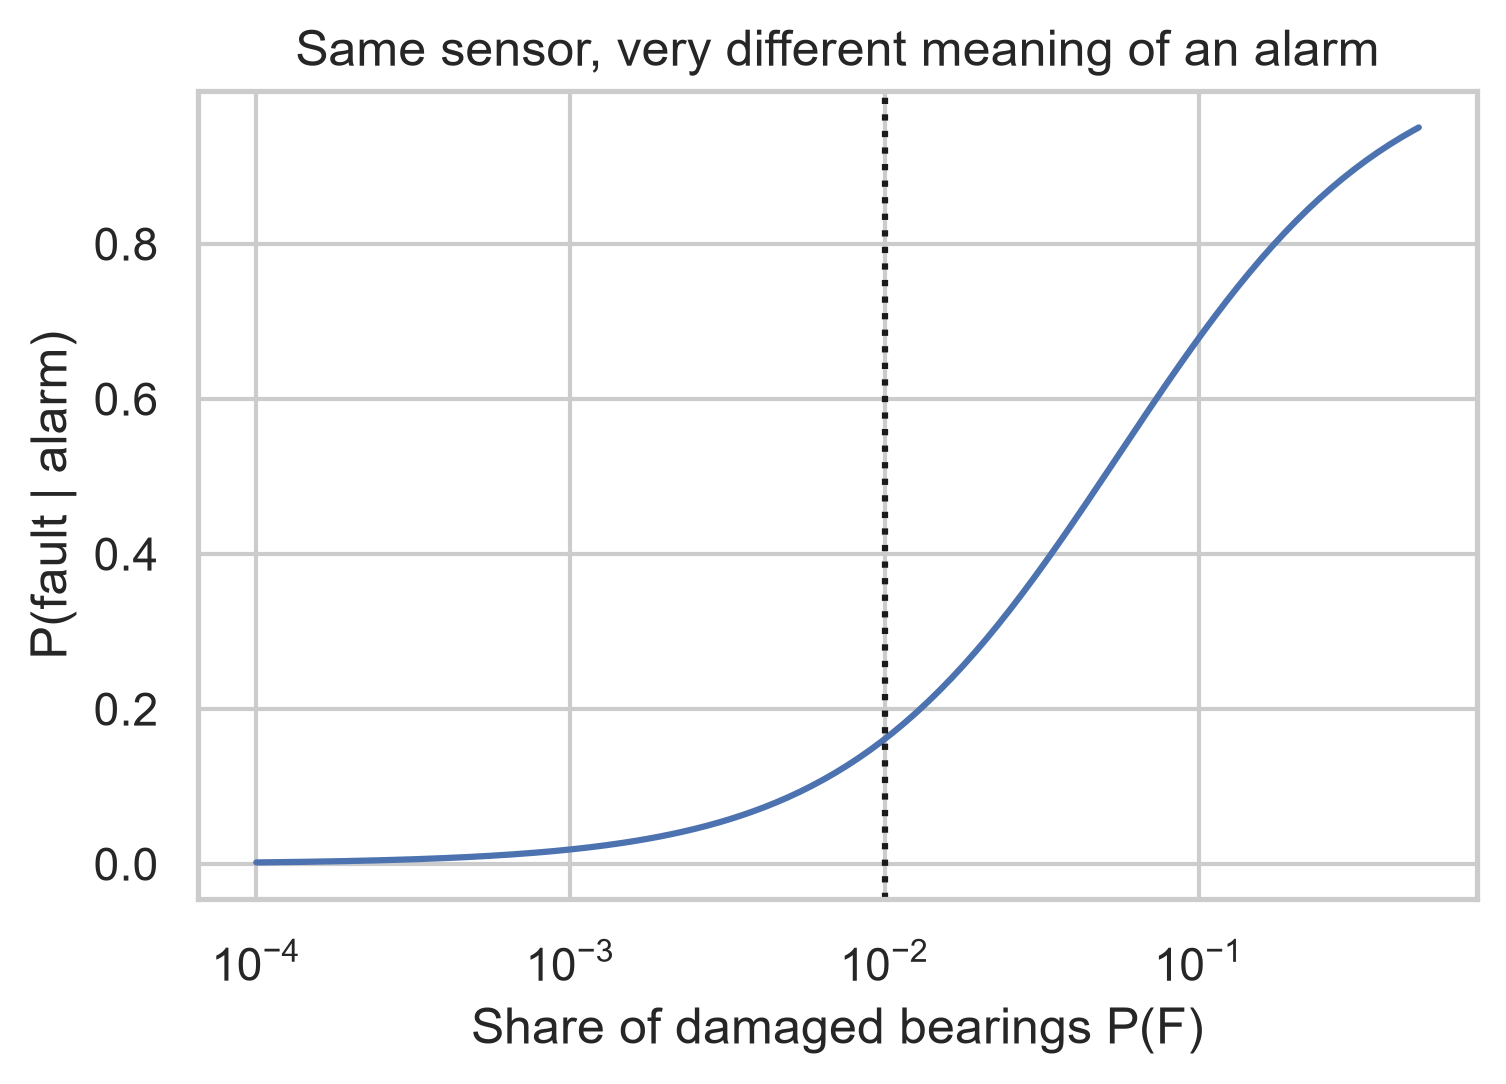
\includegraphics[keepaspectratio]{notebooks/03-uncertainty_files/figure-pdf/cell-8-output-1.png}}

\section{Extension: Bayesian estimation with prior
knowledge}\label{extension-bayesian-estimation-with-prior-knowledge}

\emph{Extension -- optional material, not required for the exam.}

Classical (frequentist) statistics uses only the current data. Bayesian
statistics treats an unknown parameter \(\theta\) itself as uncertain,
describes the knowledge before the experiment by a \textbf{prior
distribution} and updates it with the data to a \textbf{posterior
distribution}:

\[p(\theta \mid \text{data}) \propto p(\text{data} \mid \theta)\; p(\theta).\]

This is attractive in engineering, where tests are expensive but
experience from predecessor products exists. Example: a new product
variant is tested, 3 of 50 parts are defective. From the predecessor
product we know a defect rate of about 2 \%.

For a proportion, the \textbf{beta distribution} is a convenient prior:
with prior \(\text{Beta}(a, b)\) and \(k\) defects in \(n\) parts, the
posterior is again a beta distribution,
\(\text{Beta}(a + k,\; b + n - k)\). (We write \(a, b\) for the beta
parameters to avoid confusion with the Weibull shape \(\beta\).) The
prior mean is \(a/(a+b)\), so \(\text{Beta}(2, 98)\) has mean
\(2/(2+98) = 2\,\%\) and carries roughly the weight of 100 previously
inspected parts.

\begin{Shaded}
\begin{Highlighting}[]
\NormalTok{k, n }\OperatorTok{=} \DecValTok{3}\NormalTok{, }\DecValTok{50}                       \CommentTok{\# new tests: defects, parts}
\NormalTok{a0, b0 }\OperatorTok{=} \DecValTok{2}\NormalTok{, }\DecValTok{98}                     \CommentTok{\# prior from the predecessor product}
\NormalTok{a1, b1 }\OperatorTok{=}\NormalTok{ a0 }\OperatorTok{+}\NormalTok{ k, b0 }\OperatorTok{+}\NormalTok{ n }\OperatorTok{{-}}\NormalTok{ k        }\CommentTok{\# posterior}

\NormalTok{p }\OperatorTok{=}\NormalTok{ np.linspace(}\DecValTok{0}\NormalTok{, }\FloatTok{0.20}\NormalTok{, }\DecValTok{500}\NormalTok{)}
\NormalTok{plt.plot(p, stats.beta.pdf(p, a0, b0), label}\OperatorTok{=}\StringTok{"prior (predecessor)"}\NormalTok{)}
\NormalTok{plt.plot(p, stats.beta.pdf(p, }\DecValTok{1} \OperatorTok{+}\NormalTok{ k, }\DecValTok{1} \OperatorTok{+}\NormalTok{ n }\OperatorTok{{-}}\NormalTok{ k), label}\OperatorTok{=}\StringTok{"data only (flat prior)"}\NormalTok{)}
\NormalTok{plt.plot(p, stats.beta.pdf(p, a1, b1), label}\OperatorTok{=}\StringTok{"posterior"}\NormalTok{)}
\NormalTok{plt.xlabel(}\StringTok{"Defect rate"}\NormalTok{)}\OperatorTok{;}\NormalTok{ plt.ylabel(}\StringTok{"Density"}\NormalTok{)}\OperatorTok{;}\NormalTok{ plt.legend()}
\NormalTok{plt.show()}

\NormalTok{ci\_freq }\OperatorTok{=}\NormalTok{ stats.binomtest(k, n).proportion\_ci(}\FloatTok{0.95}\NormalTok{)}
\BuiltInTok{print}\NormalTok{(}\SpecialStringTok{f"Frequentist: }\SpecialCharTok{\{}\NormalTok{k}\OperatorTok{/}\NormalTok{n}\SpecialCharTok{:.1\%\}}\SpecialStringTok{, 95 \% CI [}\SpecialCharTok{\{}\NormalTok{ci\_freq}\SpecialCharTok{.}\NormalTok{low}\SpecialCharTok{:.1\%\}}\SpecialStringTok{, }\SpecialCharTok{\{}\NormalTok{ci\_freq}\SpecialCharTok{.}\NormalTok{high}\SpecialCharTok{:.1\%\}}\SpecialStringTok{]"}\NormalTok{)}
\NormalTok{lo, hi }\OperatorTok{=}\NormalTok{ stats.beta.interval(}\FloatTok{0.95}\NormalTok{, a1, b1)}
\BuiltInTok{print}\NormalTok{(}\SpecialStringTok{f"Bayesian:    }\SpecialCharTok{\{}\NormalTok{a1}\OperatorTok{/}\NormalTok{(a1}\OperatorTok{+}\NormalTok{b1)}\SpecialCharTok{:.1\%\}}\SpecialStringTok{, 95 \% credible interval [}\SpecialCharTok{\{}\NormalTok{lo}\SpecialCharTok{:.1\%\}}\SpecialStringTok{, }\SpecialCharTok{\{}\NormalTok{hi}\SpecialCharTok{:.1\%\}}\SpecialStringTok{]"}\NormalTok{)}
\end{Highlighting}
\end{Shaded}

\pandocbounded{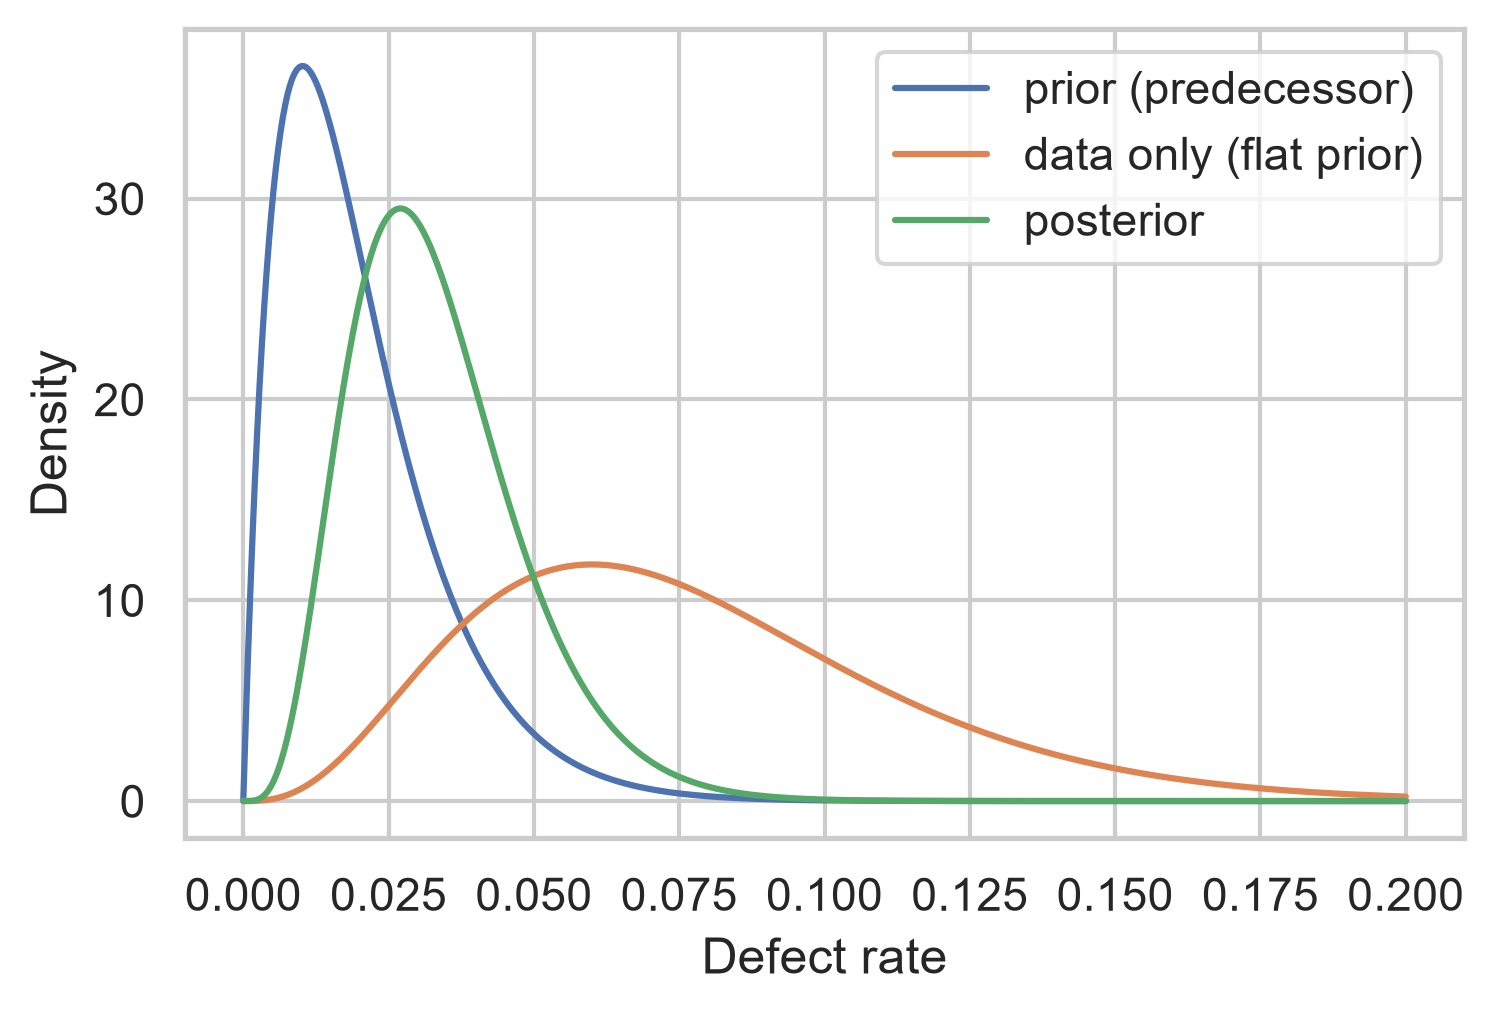
\includegraphics[keepaspectratio]{notebooks/03-uncertainty_files/figure-pdf/cell-9-output-1.png}}

\begin{verbatim}
Frequentist: 6.0%, 95 % CI [1.3%, 16.5%]
Bayesian:    3.3%, 95 % credible interval [1.1%, 6.7%]
\end{verbatim}

\textbf{Discussion.} The posterior lies between prior and data: the new
tests suggest a higher defect rate than the predecessor, but 50 parts
are not enough to overrule the experience from 100 parts completely. The
Bayesian \textbf{credible interval} has the intuitive interpretation
that the classical confidence interval lacks: given prior and data, the
defect rate lies in this interval with 95 \% probability. The price is
that the result depends on the prior -- which must therefore be
justified and documented. Whether the predecessor is really comparable
is an engineering judgement, not a statistical one.

\begin{tcolorbox}[enhanced jigsaw, colframe=quarto-callout-important-color-frame, toprule=.15mm, rightrule=.15mm, title=\textcolor{quarto-callout-important-color}{\faExclamation}\hspace{0.5em}{Key takeaways}, colbacktitle=quarto-callout-important-color!10!white, left=2mm, titlerule=0mm, bottomtitle=1mm, toptitle=1mm, opacityback=0, bottomrule=.15mm, breakable, arc=.35mm, opacitybacktitle=0.6, colback=white, coltitle=black, leftrule=.75mm]

\begin{itemize}
\tightlist
\item
  Distributions are modelling choices; physics (sum, product, weakest
  link) guides the choice, probability plots check it.
\item
  The Weibull shape parameter distinguishes early failures, random
  failures and wear-out -- and decides whether preventive maintenance
  makes sense.
\item
  Confidence intervals quantify the uncertainty of an estimate; the
  bootstrap provides them for almost any statistic.
\item
  Bayes' theorem: with rare events, even good detectors produce mostly
  false alarms.
\end{itemize}

\end{tcolorbox}

\section{Exercises}\label{exercises-2}

\begin{enumerate}
\def\labelenumi{\arabic{enumi}.}
\tightlist
\item
  Fit a lognormal, a normal and a three-parameter Weibull distribution
  (free location parameter) to the lifetimes. Compare the fits with
  probability plots and the Kolmogorov--Smirnov statistic.
\item
  Use the bootstrap to compute a 95 \% confidence interval for the B10
  life. Why is it much wider (relative to the estimate) than the
  interval for the mean?
\item
  How does the width of the confidence interval of the mean change if
  only 20 engines are available? Simulate it by drawing many random
  subsamples of 20 engines.
\item
  Interpret the shape parameter for the maintenance strategy: does
  preventive replacement make sense? At which age would you replace an
  engine if at most 5 \% of the engines may fail before replacement?
\item
  The fault share in a well-maintained fleet is only 0.1 \%. How
  reliable is an alarm of the monitoring system above? Which false alarm
  rate would be needed to reach \(P(F \mid A) = 50\,\%\)?
\item
  (Extension) Repeat the defect-rate analysis with a weak prior
  Beta(0.2, 9.8) and a strong prior Beta(20, 980). When does the prior
  dominate, when the data?
\end{enumerate}

\subsection{Solutions}\label{solutions-2}

\begin{tcolorbox}[enhanced jigsaw, colframe=quarto-callout-caution-color-frame, toprule=.15mm, rightrule=.15mm, title=\textcolor{quarto-callout-caution-color}{\faFire}\hspace{0.5em}{Solution to Exercise 1}, colbacktitle=quarto-callout-caution-color!10!white, left=2mm, titlerule=0mm, bottomtitle=1mm, toptitle=1mm, opacityback=0, bottomrule=.15mm, breakable, arc=.35mm, opacitybacktitle=0.6, colback=white, coltitle=black, leftrule=.75mm]

\begin{Shaded}
\begin{Highlighting}[]
\NormalTok{fits }\OperatorTok{=}\NormalTok{ \{}
    \StringTok{"Weibull (2p)"}\NormalTok{: (stats.weibull\_min, stats.weibull\_min.fit(lifetimes, floc}\OperatorTok{=}\DecValTok{0}\NormalTok{)),}
    \StringTok{"Weibull (3p)"}\NormalTok{: (stats.weibull\_min, stats.weibull\_min.fit(lifetimes)),}
    \StringTok{"lognormal"}\NormalTok{:    (stats.lognorm, stats.lognorm.fit(lifetimes, floc}\OperatorTok{=}\DecValTok{0}\NormalTok{)),}
    \StringTok{"normal"}\NormalTok{:       (stats.norm, stats.norm.fit(lifetimes)),}
\NormalTok{\}}
\NormalTok{fig, axes }\OperatorTok{=}\NormalTok{ plt.subplots(}\DecValTok{1}\NormalTok{, }\DecValTok{4}\NormalTok{, figsize}\OperatorTok{=}\NormalTok{(}\DecValTok{16}\NormalTok{, }\DecValTok{4}\NormalTok{))}
\ControlFlowTok{for}\NormalTok{ ax, (name, (dist, params)) }\KeywordTok{in} \BuiltInTok{zip}\NormalTok{(axes, fits.items()):}
\NormalTok{    stats.probplot(lifetimes, dist}\OperatorTok{=}\NormalTok{dist, sparams}\OperatorTok{=}\NormalTok{params, plot}\OperatorTok{=}\NormalTok{ax)}
\NormalTok{    ks }\OperatorTok{=}\NormalTok{ stats.kstest(lifetimes, dist.cdf, args}\OperatorTok{=}\NormalTok{params)}
\NormalTok{    ax.set\_title(}\SpecialStringTok{f"}\SpecialCharTok{\{}\NormalTok{name}\SpecialCharTok{\}}\CharTok{\textbackslash{}n}\SpecialStringTok{KS D = }\SpecialCharTok{\{}\NormalTok{ks}\SpecialCharTok{.}\NormalTok{statistic}\SpecialCharTok{:.3f\}}\SpecialStringTok{"}\NormalTok{)}
\NormalTok{plt.tight\_layout()}\OperatorTok{;}\NormalTok{ plt.show()}
\end{Highlighting}
\end{Shaded}

\pandocbounded{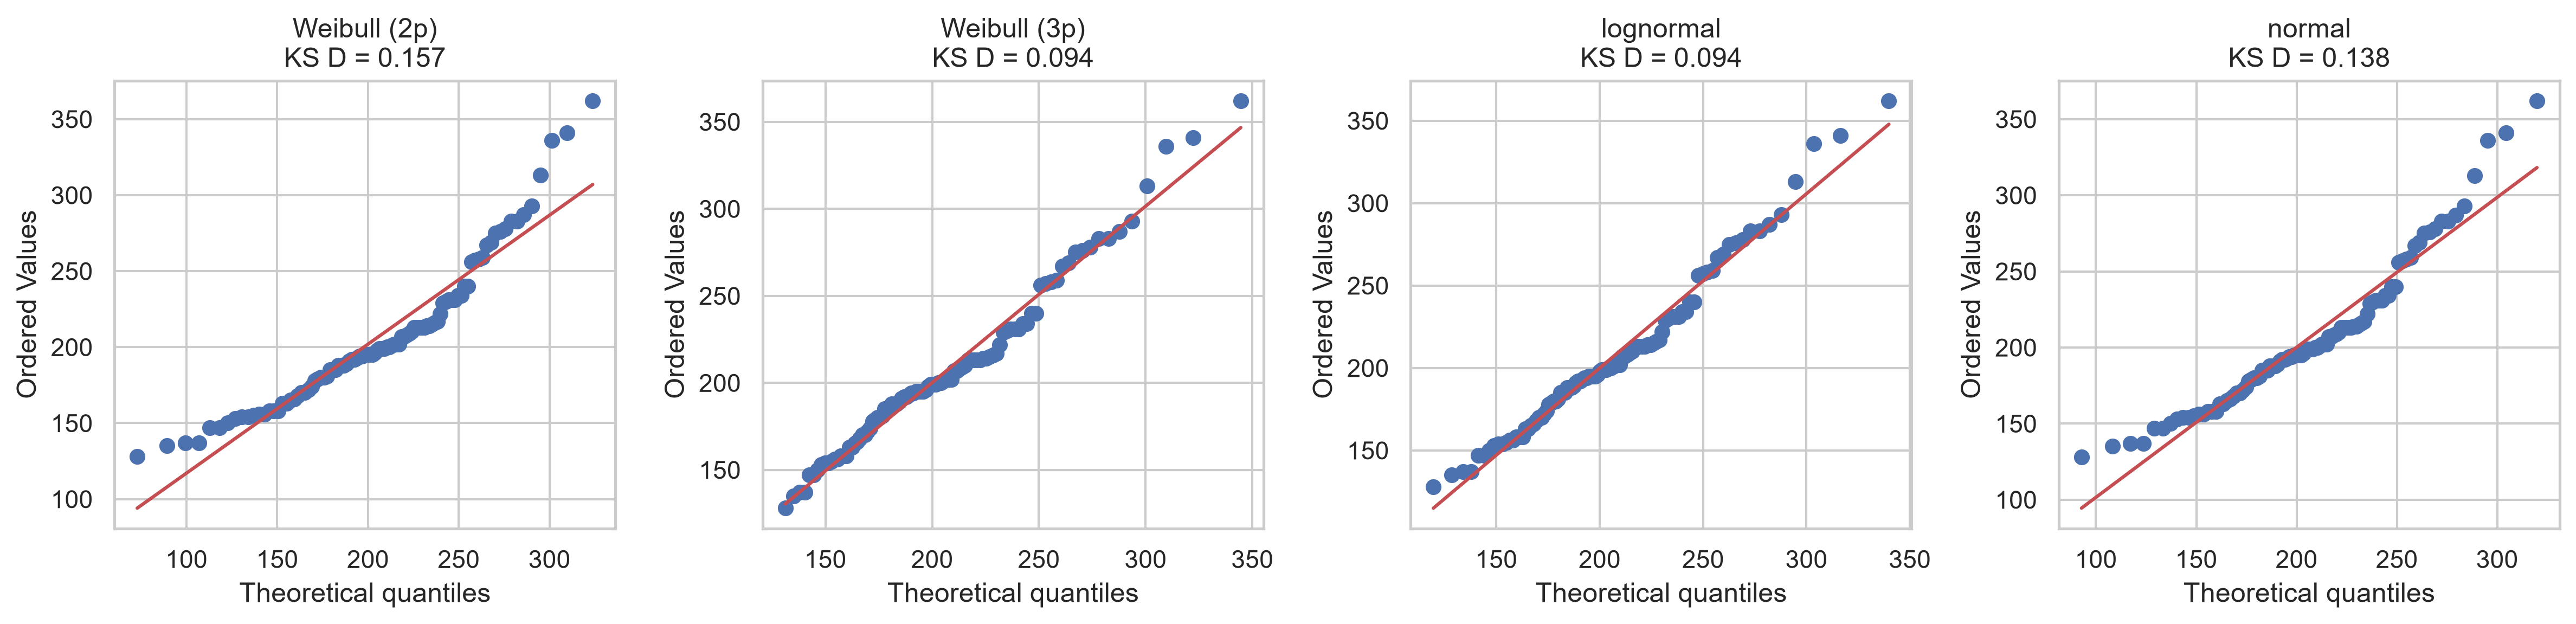
\includegraphics[keepaspectratio]{notebooks/03-uncertainty_files/figure-pdf/cell-10-output-1.png}}

The model with the smallest KS statistic and the straightest probability
plot fits best. The three-parameter Weibull has one more parameter and
therefore always fits at least as well as the two-parameter version; its
location parameter estimates a failure-free time. Caution: the p-values
of the KS test are not valid when the parameters were estimated from the
same data, so use the statistic for comparison only. With 100
observations, several distributions usually fit acceptably -- the choice
should also be guided by physics (Weibull for wear-out).

\end{tcolorbox}

\begin{tcolorbox}[enhanced jigsaw, colframe=quarto-callout-caution-color-frame, toprule=.15mm, rightrule=.15mm, title=\textcolor{quarto-callout-caution-color}{\faFire}\hspace{0.5em}{Solution to Exercise 2}, colbacktitle=quarto-callout-caution-color!10!white, left=2mm, titlerule=0mm, bottomtitle=1mm, toptitle=1mm, opacityback=0, bottomrule=.15mm, breakable, arc=.35mm, opacitybacktitle=0.6, colback=white, coltitle=black, leftrule=.75mm]

\begin{Shaded}
\begin{Highlighting}[]
\KeywordTok{def}\NormalTok{ b10\_stat(x):}
\NormalTok{    c, \_, scale }\OperatorTok{=}\NormalTok{ stats.weibull\_min.fit(x, floc}\OperatorTok{=}\DecValTok{0}\NormalTok{)}
    \ControlFlowTok{return}\NormalTok{ stats.weibull\_min.ppf(}\FloatTok{0.10}\NormalTok{, c, scale}\OperatorTok{=}\NormalTok{scale)}

\NormalTok{boot\_b10 }\OperatorTok{=}\NormalTok{ stats.bootstrap((lifetimes.values,), b10\_stat, n\_resamples}\OperatorTok{=}\DecValTok{1000}\NormalTok{,}
\NormalTok{                           method}\OperatorTok{=}\StringTok{"percentile"}\NormalTok{, random\_state}\OperatorTok{=}\DecValTok{0}\NormalTok{)}
\NormalTok{lo, hi }\OperatorTok{=}\NormalTok{ boot\_b10.confidence\_interval}
\BuiltInTok{print}\NormalTok{(}\SpecialStringTok{f"B10 = }\SpecialCharTok{\{}\NormalTok{b10}\SpecialCharTok{:.0f\}}\SpecialStringTok{ cycles, 95 \% CI [}\SpecialCharTok{\{}\NormalTok{lo}\SpecialCharTok{:.0f\}}\SpecialStringTok{, }\SpecialCharTok{\{}\NormalTok{hi}\SpecialCharTok{:.0f\}}\SpecialStringTok{]  (relative width }\SpecialCharTok{\{}\NormalTok{(hi }\OperatorTok{{-}}\NormalTok{ lo) }\OperatorTok{/}\NormalTok{ b10}\SpecialCharTok{:.0\%\}}\SpecialStringTok{)"}\NormalTok{)}
\BuiltInTok{print}\NormalTok{(}\SpecialStringTok{f"Mean: relative width }\SpecialCharTok{\{}\NormalTok{(ci\_t[}\DecValTok{1}\NormalTok{] }\OperatorTok{{-}}\NormalTok{ ci\_t[}\DecValTok{0}\NormalTok{]) }\OperatorTok{/}\NormalTok{ lifetimes}\SpecialCharTok{.}\NormalTok{mean()}\SpecialCharTok{:.0\%\}}\SpecialStringTok{"}\NormalTok{)}
\end{Highlighting}
\end{Shaded}

\begin{verbatim}
B10 = 135 cycles, 95 % CI [127, 146]  (relative width 14%)
Mean: relative width 9%
\end{verbatim}

The B10 life is a statement about the \textbf{lower tail} of the
distribution, where only about 10 of the 100 engines contribute
information. In addition, it depends on two estimated parameters, and
the shape parameter enters as an exponent. The mean uses all
observations equally. Reliability figures in the tails are therefore
always much more uncertain than averages -- a reason for large safety
factors.

\end{tcolorbox}

\begin{tcolorbox}[enhanced jigsaw, colframe=quarto-callout-caution-color-frame, toprule=.15mm, rightrule=.15mm, title=\textcolor{quarto-callout-caution-color}{\faFire}\hspace{0.5em}{Solution to Exercise 3}, colbacktitle=quarto-callout-caution-color!10!white, left=2mm, titlerule=0mm, bottomtitle=1mm, toptitle=1mm, opacityback=0, bottomrule=.15mm, breakable, arc=.35mm, opacitybacktitle=0.6, colback=white, coltitle=black, leftrule=.75mm]

\begin{Shaded}
\begin{Highlighting}[]
\NormalTok{rng }\OperatorTok{=}\NormalTok{ np.random.default\_rng(}\DecValTok{0}\NormalTok{)}
\NormalTok{widths }\OperatorTok{=}\NormalTok{ []}
\ControlFlowTok{for}\NormalTok{ \_ }\KeywordTok{in} \BuiltInTok{range}\NormalTok{(}\DecValTok{2000}\NormalTok{):}
\NormalTok{    sub }\OperatorTok{=}\NormalTok{ rng.choice(lifetimes.values, size}\OperatorTok{=}\DecValTok{20}\NormalTok{, replace}\OperatorTok{=}\VariableTok{False}\NormalTok{)}
\NormalTok{    lo\_, hi\_ }\OperatorTok{=}\NormalTok{ stats.t.interval(}\FloatTok{0.95}\NormalTok{, df}\OperatorTok{=}\DecValTok{19}\NormalTok{, loc}\OperatorTok{=}\NormalTok{sub.mean(), scale}\OperatorTok{=}\NormalTok{stats.sem(sub))}
\NormalTok{    widths.append(hi\_ }\OperatorTok{{-}}\NormalTok{ lo\_)}
\BuiltInTok{print}\NormalTok{(}\SpecialStringTok{f"n = 100: width }\SpecialCharTok{\{}\NormalTok{ci\_t[}\DecValTok{1}\NormalTok{] }\OperatorTok{{-}}\NormalTok{ ci\_t[}\DecValTok{0}\NormalTok{]}\SpecialCharTok{:.1f\}}\SpecialStringTok{ cycles"}\NormalTok{)}
\BuiltInTok{print}\NormalTok{(}\SpecialStringTok{f"n = 20:  mean width }\SpecialCharTok{\{}\NormalTok{np}\SpecialCharTok{.}\NormalTok{mean(widths)}\SpecialCharTok{:.1f\}}\SpecialStringTok{ cycles (ratio }\SpecialCharTok{\{}\NormalTok{np}\SpecialCharTok{.}\NormalTok{mean(widths) }\OperatorTok{/}\NormalTok{ (ci\_t[}\DecValTok{1}\NormalTok{] }\OperatorTok{{-}}\NormalTok{ ci\_t[}\DecValTok{0}\NormalTok{])}\SpecialCharTok{:.2f\}}\SpecialStringTok{)"}\NormalTok{)}
\end{Highlighting}
\end{Shaded}

\begin{verbatim}
n = 100: width 18.4 cycles
n = 20:  mean width 42.6 cycles (ratio 2.32)
\end{verbatim}

The width scales approximately with \(1/\sqrt{n}\), so going from 100 to
20 engines should make the interval about \(\sqrt{5} \approx 2.2\) times
wider; the t-quantile for 19 degrees of freedom (2.09 instead of 1.98)
adds a little more. (Subsampling without replacement from only 100
engines slightly reduces the spread, so the simulated ratio can be a bit
smaller.)

\end{tcolorbox}

\begin{tcolorbox}[enhanced jigsaw, colframe=quarto-callout-caution-color-frame, toprule=.15mm, rightrule=.15mm, title=\textcolor{quarto-callout-caution-color}{\faFire}\hspace{0.5em}{Solution to Exercise 4}, colbacktitle=quarto-callout-caution-color!10!white, left=2mm, titlerule=0mm, bottomtitle=1mm, toptitle=1mm, opacityback=0, bottomrule=.15mm, breakable, arc=.35mm, opacitybacktitle=0.6, colback=white, coltitle=black, leftrule=.75mm]

\begin{Shaded}
\begin{Highlighting}[]
\NormalTok{t05 }\OperatorTok{=}\NormalTok{ stats.weibull\_min.ppf(}\FloatTok{0.05}\NormalTok{, beta, scale}\OperatorTok{=}\NormalTok{eta)}
\BuiltInTok{print}\NormalTok{(}\SpecialStringTok{f"beta = }\SpecialCharTok{\{}\NormalTok{beta}\SpecialCharTok{:.2f\}}\SpecialStringTok{ \textgreater{} 1 {-}\textgreater{} wear{-}out; replacement age for 5 \% failures: }\SpecialCharTok{\{}\NormalTok{t05}\SpecialCharTok{:.0f\}}\SpecialStringTok{ cycles"}\NormalTok{)}
\end{Highlighting}
\end{Shaded}

\begin{verbatim}
beta = 4.41 > 1 -> wear-out; replacement age for 5 % failures: 115 cycles
\end{verbatim}

Since \(\beta > 1\), the failure rate increases with age, so preventive
replacement reduces failures. The replacement age for at most 5 \%
failures is the 5 \% quantile \(B_5 = \eta(-\ln 0.95)^{1/\beta}\). Given
the large uncertainty of tail estimates (Exercise 2), one would in
practice use the lower confidence bound of \(B_5\) rather than the point
estimate. Whether replacement is economical depends additionally on the
cost ratio of planned replacement and unplanned failure.

\end{tcolorbox}

\begin{tcolorbox}[enhanced jigsaw, colframe=quarto-callout-caution-color-frame, toprule=.15mm, rightrule=.15mm, title=\textcolor{quarto-callout-caution-color}{\faFire}\hspace{0.5em}{Solution to Exercise 5}, colbacktitle=quarto-callout-caution-color!10!white, left=2mm, titlerule=0mm, bottomtitle=1mm, toptitle=1mm, opacityback=0, bottomrule=.15mm, breakable, arc=.35mm, opacitybacktitle=0.6, colback=white, coltitle=black, leftrule=.75mm]

With \(P(F) = 0.001\):
\[P(F \mid A) = \frac{0.95 \cdot 0.001}{0.95 \cdot 0.001 + 0.05 \cdot 0.999} \approx 0.019,\]
i.e.~only about 2 \% of the alarms are real. For \(P(F \mid A) = 0.5\)
we need \(0.95 \cdot 0.001 = q \cdot 0.999\), where
\(q = P(A \mid \bar F)\) is the false alarm rate, so
\(q \approx 0.00095\) -- roughly one false alarm per thousand healthy
bearings. The better the fleet, the more specific the monitoring must
be.

\end{tcolorbox}

\begin{tcolorbox}[enhanced jigsaw, colframe=quarto-callout-caution-color-frame, toprule=.15mm, rightrule=.15mm, title=\textcolor{quarto-callout-caution-color}{\faFire}\hspace{0.5em}{Solution to Exercise 6}, colbacktitle=quarto-callout-caution-color!10!white, left=2mm, titlerule=0mm, bottomtitle=1mm, toptitle=1mm, opacityback=0, bottomrule=.15mm, breakable, arc=.35mm, opacitybacktitle=0.6, colback=white, coltitle=black, leftrule=.75mm]

\begin{Shaded}
\begin{Highlighting}[]
\ControlFlowTok{for}\NormalTok{ name, (a, b) }\KeywordTok{in}\NormalTok{ \{}\StringTok{"weak"}\NormalTok{: (}\FloatTok{0.2}\NormalTok{, }\FloatTok{9.8}\NormalTok{), }\StringTok{"medium"}\NormalTok{: (}\DecValTok{2}\NormalTok{, }\DecValTok{98}\NormalTok{), }\StringTok{"strong"}\NormalTok{: (}\DecValTok{20}\NormalTok{, }\DecValTok{980}\NormalTok{)\}.items():}
\NormalTok{    post }\OperatorTok{=}\NormalTok{ stats.beta(a }\OperatorTok{+}\NormalTok{ k, b }\OperatorTok{+}\NormalTok{ n }\OperatorTok{{-}}\NormalTok{ k)}
\NormalTok{    lo\_, hi\_ }\OperatorTok{=}\NormalTok{ post.interval(}\FloatTok{0.95}\NormalTok{)}
    \BuiltInTok{print}\NormalTok{(}\SpecialStringTok{f"}\SpecialCharTok{\{}\NormalTok{name}\SpecialCharTok{:6s\}}\SpecialStringTok{ prior: posterior mean }\SpecialCharTok{\{}\NormalTok{post}\SpecialCharTok{.}\NormalTok{mean()}\SpecialCharTok{:.1\%\}}\SpecialStringTok{, 95 \% credible interval [}\SpecialCharTok{\{}\NormalTok{lo\_}\SpecialCharTok{:.1\%\}}\SpecialStringTok{, }\SpecialCharTok{\{}\NormalTok{hi\_}\SpecialCharTok{:.1\%\}}\SpecialStringTok{]"}\NormalTok{)}
\end{Highlighting}
\end{Shaded}

\begin{verbatim}
weak   prior: posterior mean 5.3%, 95 % credible interval [1.2%, 12.2%]
medium prior: posterior mean 3.3%, 95 % credible interval [1.1%, 6.7%]
strong prior: posterior mean 2.2%, 95 % credible interval [1.4%, 3.2%]
\end{verbatim}

All three priors have a mean of 2 \% but different weights (\(a + b\) =
10, 100, 1000 ``virtual parts''). The weak prior is dominated by the 50
real parts: the posterior mean is close to the observed 6 \%. The strong
prior hardly moves -- 50 parts are not enough to overrule 1,000 virtual
ones. Rule of thumb: the data dominate once \(n\) is large compared with
\(a + b\).

\end{tcolorbox}

\part{Part B -- Statistics for Engineers}

\chapter{Statistical Testing}\label{statistical-testing}

A process engineer changes the supplier of a raw material, and the mean
scrap rate in the following week is slightly lower. Is the new material
better -- or was it a good week by chance? Questions like this are
everyday engineering questions, and statistical hypothesis tests are the
standard tool to answer them. They provide a disciplined way to decide
whether an observed difference is larger than what random variation
alone would plausibly produce.

Tests are also among the most misunderstood tools of statistics. A small
p-value does not mean that an effect is large or important, and a large
p-value does not prove that there is no effect. With the big datasets of
modern production, almost every difference becomes ``significant''. This
chapter therefore puts as much weight on \textbf{effect sizes} and
\textbf{practical relevance} as on p-values.

\textbf{Scenario: the consultant's bonus}

A gas turbine power plant hired a consultant in 2011 to reduce its NOx
emissions through better operating practices. The contract promises a
bonus if the emissions in 2015 are ``demonstrably and relevantly lower''
than in 2011; the contract defines \emph{relevant} as a reduction of at
least 5 \% of the 2011 mean. The consultant presents a test with a tiny
p-value and asks for payment. You are asked to review the claim for the
plant management.

\textbf{Your decision:} Confirm the claim and approve the bonus -- or
not?

\textbf{Learning goals.} After this chapter you can

\begin{itemize}
\tightlist
\item
  formulate engineering questions as statistical hypotheses,
\item
  explain test statistic, p-value, significance level, type I and type
  II errors and power,
\item
  choose and apply t-tests, ANOVA, chi-squared and non-parametric tests,
\item
  distinguish statistical significance from practical relevance (effect
  size),
\item
  recognise and correct for the multiple-testing problem,
\item
  estimate the sample size needed to detect a relevant effect.
\end{itemize}

\textbf{Datasets in this chapter}

\begin{itemize}
\tightlist
\item
  \href{https://archive.ics.uci.edu/dataset/551/gas+turbine+co+and+nox+emission+data+set}{Gas
  Turbine CO and NOx Emission (UCI)}
\item
  \href{https://archive.ics.uci.edu/dataset/601/ai4i+2020+predictive+maintenance+dataset}{AI4I
  2020 Predictive Maintenance (UCI)}
\end{itemize}

\section{The logic of a hypothesis
test}\label{the-logic-of-a-hypothesis-test}

A hypothesis test is a proof by contradiction with uncertainty. We
assume that there is \emph{no} effect and check whether the data are
compatible with this assumption.

\begin{tcolorbox}[enhanced jigsaw, colframe=quarto-callout-note-color-frame, toprule=.15mm, rightrule=.15mm, title=\textcolor{quarto-callout-note-color}{\faInfo}\hspace{0.5em}{Definition: Elements of a hypothesis test}, colbacktitle=quarto-callout-note-color!10!white, left=2mm, titlerule=0mm, bottomtitle=1mm, toptitle=1mm, opacityback=0, bottomrule=.15mm, breakable, arc=.35mm, opacitybacktitle=0.6, colback=white, coltitle=black, leftrule=.75mm]

\begin{itemize}
\tightlist
\item
  \textbf{Null hypothesis} \(H_0\): the ``nothing special'' statement,
  e.g.~\(\mu_1 = \mu_2\) (both suppliers give the same mean).
\item
  \textbf{Alternative hypothesis} \(H_1\): what we want to detect,
  e.g.~\(\mu_1 \neq \mu_2\).
\item
  \textbf{Test statistic} \(T\): a number computed from the data that
  measures the deviation from \(H_0\).
\item
  \textbf{p-value}: the probability of obtaining a test statistic at
  least as extreme as the observed one, \textbf{assuming \(H_0\) is
  true}.
\item
  \textbf{Significance level} \(\alpha\) (often 0.05): \(H_0\) is
  rejected if \(p < \alpha\).
\end{itemize}

\end{tcolorbox}

Two kinds of wrong decisions are possible:

\begin{longtable}[]{@{}
  >{\raggedright\arraybackslash}p{(\linewidth - 4\tabcolsep) * \real{0.3333}}
  >{\raggedright\arraybackslash}p{(\linewidth - 4\tabcolsep) * \real{0.3333}}
  >{\raggedright\arraybackslash}p{(\linewidth - 4\tabcolsep) * \real{0.3333}}@{}}
\toprule\noalign{}
\begin{minipage}[b]{\linewidth}\raggedright
\end{minipage} & \begin{minipage}[b]{\linewidth}\raggedright
\(H_0\) true (no effect)
\end{minipage} & \begin{minipage}[b]{\linewidth}\raggedright
\(H_0\) false (effect exists)
\end{minipage} \\
\midrule\noalign{}
\endhead
\bottomrule\noalign{}
\endlastfoot
\textbf{\(H_0\) rejected} & type I error (false alarm), probability
\(\alpha\) & correct decision, probability \(1 - \beta\) =
\textbf{power} \\
\textbf{\(H_0\) not rejected} & correct decision & type II error (missed
effect), probability \(\beta\) \\
\end{longtable}

\begin{figure}[H]

\centering{

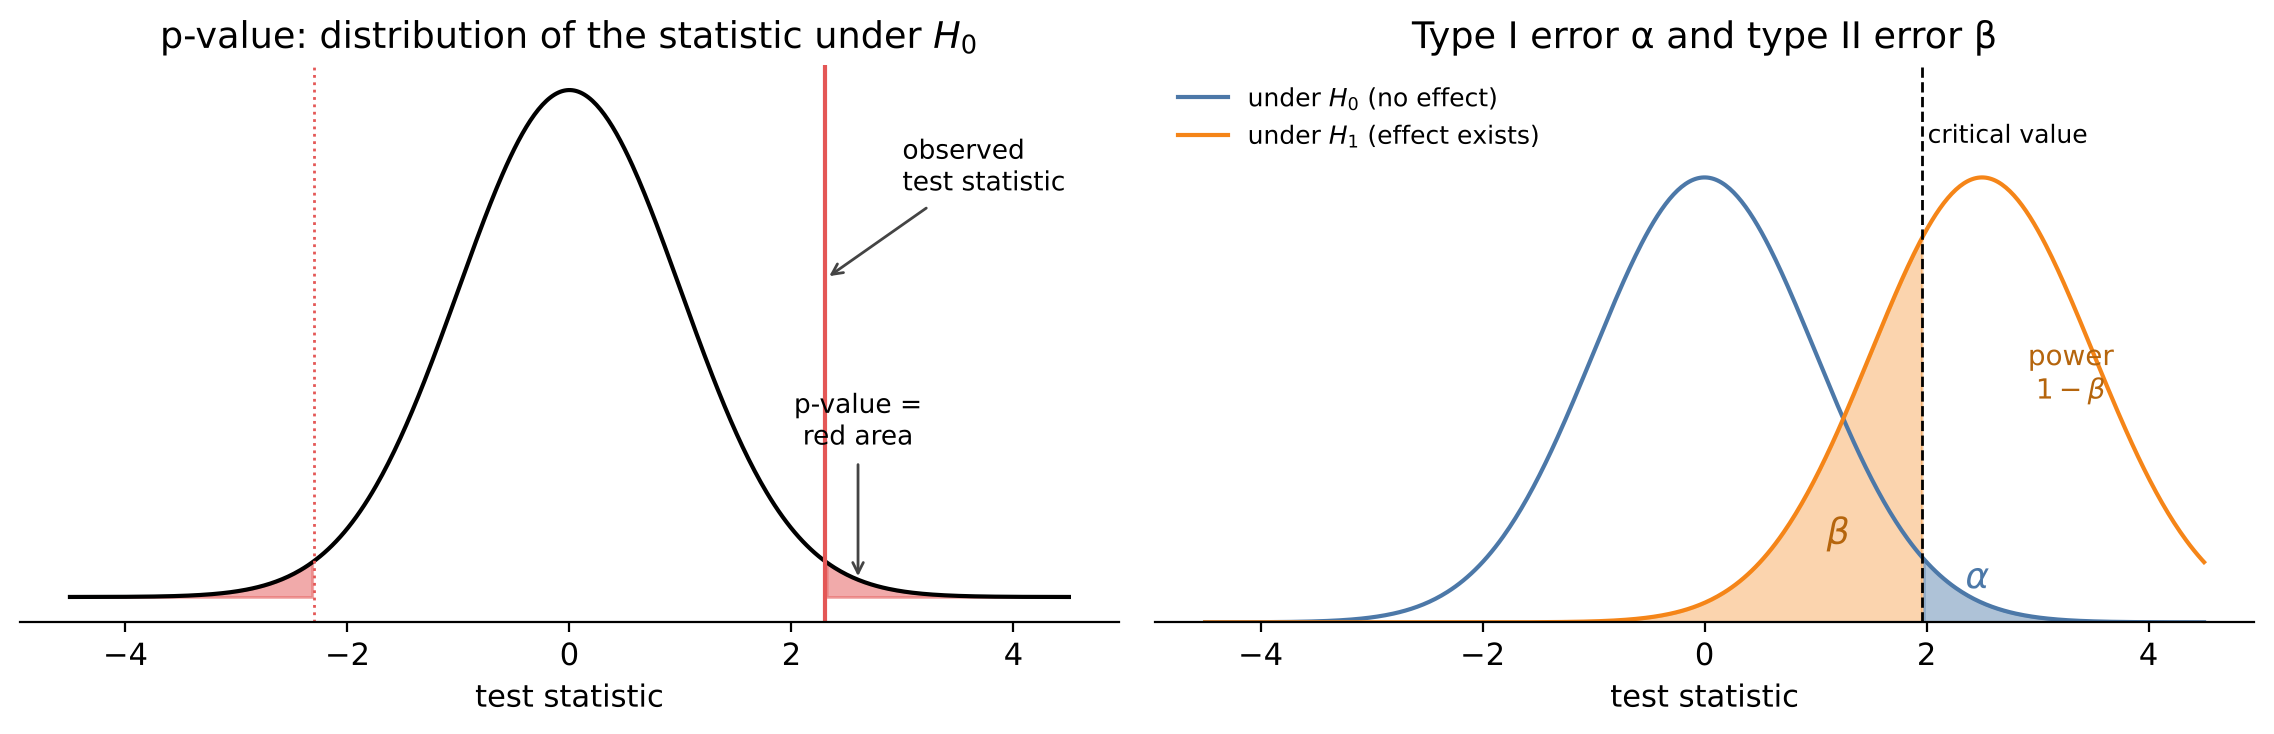
\includegraphics[width=1\linewidth,height=\textheight,keepaspectratio]{notebooks/images/pvalue-errors.png}

}

\caption{\label{fig-pvalue}Left: the p-value is the probability,
computed under the null hypothesis, of a test statistic at least as
extreme as the observed one (two-sided test). Right: the two error
types. The critical value is set such that the false alarm probability α
is 5 \%; the probability β of missing a real effect depends on the
effect size and the sample size.}

\end{figure}%

The significance level controls the false alarm rate. The power depends
on the size of the effect, the noise level and the sample size -- small
samples often have too little power to detect relevant effects.

\begin{tcolorbox}[enhanced jigsaw, colframe=quarto-callout-warning-color-frame, toprule=.15mm, rightrule=.15mm, title=\textcolor{quarto-callout-warning-color}{\faExclamationTriangle}\hspace{0.5em}{Pitfall: what the p-value is not}, colbacktitle=quarto-callout-warning-color!10!white, left=2mm, titlerule=0mm, bottomtitle=1mm, toptitle=1mm, opacityback=0, bottomrule=.15mm, breakable, arc=.35mm, opacitybacktitle=0.6, colback=white, coltitle=black, leftrule=.75mm]

\begin{itemize}
\tightlist
\item
  It is \textbf{not} the probability that \(H_0\) is true.
\item
  \(p \ge 0.05\) does \textbf{not} prove that there is no effect --
  maybe the sample was just too small (``absence of evidence is not
  evidence of absence'').
\item
  \(p < 0.05\) says nothing about the \textbf{size} or the
  \textbf{importance} of the effect.
\end{itemize}

\end{tcolorbox}

\section{Comparing two groups: the
t-test}\label{comparing-two-groups-the-t-test}

For two independent samples with means \(\bar x_1, \bar x_2\), standard
deviations \(s_1, s_2\) and sizes \(n_1, n_2\), the \textbf{Welch
t-test} uses

\[t = \frac{\bar x_1 - \bar x_2}{\sqrt{s_1^2/n_1 + s_2^2/n_2}}.\]

Under \(H_0\), \(t\) follows approximately a t-distribution. Welch's
version does not assume equal variances and should be the default (the
classical Student t-test assumes them). The test assumes independent
observations and approximately normal data -- for large samples, the
central limit theorem makes the normality assumption less critical.

\begin{tcolorbox}[enhanced jigsaw, colframe=quarto-callout-important-color-frame, toprule=.15mm, rightrule=.15mm, title=\textcolor{quarto-callout-important-color}{\faExclamation}\hspace{0.5em}{Tests and confidence intervals are two sides of one coin}, colbacktitle=quarto-callout-important-color!10!white, left=2mm, titlerule=0mm, bottomtitle=1mm, toptitle=1mm, opacityback=0, bottomrule=.15mm, breakable, arc=.35mm, opacitybacktitle=0.6, colback=white, coltitle=black, leftrule=.75mm]

A two-sided test at level \(\alpha = 0.05\) rejects
\(H_0: \mu_1 - \mu_2 = 0\) exactly when the 95 \% confidence interval
for \(\mu_1 - \mu_2\) does not contain 0. The interval is more
informative: it shows not only \emph{whether} there is a difference but
also \emph{how large} it plausibly is. Report intervals whenever
possible.

\end{tcolorbox}

\section{More than two groups, categories and non-normal
data}\label{more-than-two-groups-categories-and-non-normal-data}

\begin{longtable}[]{@{}
  >{\raggedright\arraybackslash}p{(\linewidth - 6\tabcolsep) * \real{0.2500}}
  >{\raggedright\arraybackslash}p{(\linewidth - 6\tabcolsep) * \real{0.2500}}
  >{\raggedright\arraybackslash}p{(\linewidth - 6\tabcolsep) * \real{0.2500}}
  >{\raggedright\arraybackslash}p{(\linewidth - 6\tabcolsep) * \real{0.2500}}@{}}
\toprule\noalign{}
\begin{minipage}[b]{\linewidth}\raggedright
Question
\end{minipage} & \begin{minipage}[b]{\linewidth}\raggedright
Data
\end{minipage} & \begin{minipage}[b]{\linewidth}\raggedright
Test
\end{minipage} & \begin{minipage}[b]{\linewidth}\raggedright
SciPy
\end{minipage} \\
\midrule\noalign{}
\endhead
\bottomrule\noalign{}
\endlastfoot
Do two groups differ in their mean? & continuous, approx. normal & Welch
t-test & \texttt{ttest\_ind(equal\_var=False)} \\
\ldots{} without normality assumption & continuous / ordinal &
Mann--Whitney U & \texttt{mannwhitneyu} \\
Paired measurements (before/after on the same parts) & continuous &
paired t-test / Wilcoxon & \texttt{ttest\_rel} / \texttt{wilcoxon} \\
Do \(k\) groups differ? & continuous & one-way ANOVA / Kruskal--Wallis &
\texttt{f\_oneway} / \texttt{kruskal} \\
Are two categorical variables related? & counts in a contingency table &
chi-squared test & \texttt{chi2\_contingency} \\
\end{longtable}

The \textbf{one-way ANOVA} (analysis of variance) compares the variation
\emph{between} group means with the variation \emph{within} the groups:

\[F = \frac{\text{variance between groups}}{\text{variance within groups}} = \frac{\sum_j n_j(\bar x_j - \bar x)^2/(k-1)}{\sum_j \sum_i (x_{ij} - \bar x_j)^2/(N-k)}.\]

Here \(x_{ij}\) is observation \(i\) in group \(j\), \(\bar x_j\) the
mean of group \(j\) with \(n_j\) observations, \(\bar x\) the overall
mean, \(k\) the number of groups and \(N\) the total number of
observations. A large \(F\) indicates that at least one group mean
differs. ANOVA does not say \emph{which} one -- this requires pairwise
comparisons, which lead to the multiple-testing problem below.

The \textbf{chi-squared test} compares the observed counts \(O\) in a
contingency table with the counts \(E\) expected if the variables were
independent: \(\chi^2 = \sum (O - E)^2/E\).

\section{Effect size and practical
relevance}\label{effect-size-and-practical-relevance}

\begin{tcolorbox}[enhanced jigsaw, colframe=quarto-callout-note-color-frame, toprule=.15mm, rightrule=.15mm, title=\textcolor{quarto-callout-note-color}{\faInfo}\hspace{0.5em}{Definition: Cohen's d}, colbacktitle=quarto-callout-note-color!10!white, left=2mm, titlerule=0mm, bottomtitle=1mm, toptitle=1mm, opacityback=0, bottomrule=.15mm, breakable, arc=.35mm, opacitybacktitle=0.6, colback=white, coltitle=black, leftrule=.75mm]

The standardised mean difference
\[d = \frac{\bar x_1 - \bar x_2}{s_p}, \qquad s_p = \sqrt{\frac{s_1^2 + s_2^2}{2}},\]
expresses a difference in units of the standard deviation. Rough
conventions: \(|d| \approx 0.2\) small, \(0.5\) medium, \(0.8\) large.

\end{tcolorbox}

In engineering, the most meaningful effect size is often the raw
difference in physical units, compared with a tolerance or a
requirement: ``the mean diameter differs by 0.2 µm, the tolerance is ±20
µm''.

\begin{tcolorbox}[enhanced jigsaw, colframe=quarto-callout-warning-color-frame, toprule=.15mm, rightrule=.15mm, title=\textcolor{quarto-callout-warning-color}{\faExclamationTriangle}\hspace{0.5em}{Pitfall: significance with large samples}, colbacktitle=quarto-callout-warning-color!10!white, left=2mm, titlerule=0mm, bottomtitle=1mm, toptitle=1mm, opacityback=0, bottomrule=.15mm, breakable, arc=.35mm, opacitybacktitle=0.6, colback=white, coltitle=black, leftrule=.75mm]

The standard error shrinks with \(1/\sqrt{n}\). With thousands of
observations, differences far too small to matter become highly
significant. With big data, always ask: \emph{Is the difference large
enough to matter for the process?}

\end{tcolorbox}

\section{The multiple-testing
problem}\label{the-multiple-testing-problem}

If we perform 20 independent tests at \(\alpha = 0.05\) and no effect
exists anywhere, we still expect one ``significant'' result by chance.
The probability of at least one false alarm is
\(1 - 0.95^{20} \approx 64\,\%\).

\begin{tcolorbox}[enhanced jigsaw, colframe=quarto-callout-tip-color-frame, toprule=.15mm, rightrule=.15mm, title=\textcolor{quarto-callout-tip-color}{\faLightbulb}\hspace{0.5em}{Correcting for multiple tests}, colbacktitle=quarto-callout-tip-color!10!white, left=2mm, titlerule=0mm, bottomtitle=1mm, toptitle=1mm, opacityback=0, bottomrule=.15mm, breakable, arc=.35mm, opacitybacktitle=0.6, colback=white, coltitle=black, leftrule=.75mm]

The simplest correction is \textbf{Bonferroni}: with \(m\) tests, use
\(\alpha/m\) for each. It is conservative. The \textbf{Holm} method is
uniformly better and equally simple. Both are available in
\texttt{statsmodels.stats.multitest.multipletests}. Most importantly:
decide \emph{before} looking at the data which comparisons you will
test.

\end{tcolorbox}

\begin{Shaded}
\begin{Highlighting}[]
\CommentTok{\# Setup: works locally and in Google Colab}
\ImportTok{import}\NormalTok{ importlib.util, subprocess, sys}
\ControlFlowTok{for}\NormalTok{ pkg }\KeywordTok{in}\NormalTok{ [}\StringTok{"ucimlrepo"}\NormalTok{]:}
    \ControlFlowTok{if}\NormalTok{ importlib.util.find\_spec(pkg) }\KeywordTok{is} \VariableTok{None}\NormalTok{:}
\NormalTok{        subprocess.run([sys.executable, }\StringTok{"{-}m"}\NormalTok{, }\StringTok{"pip"}\NormalTok{, }\StringTok{"install"}\NormalTok{, }\StringTok{"{-}q"}\NormalTok{, pkg], check}\OperatorTok{=}\VariableTok{True}\NormalTok{)}

\ImportTok{import}\NormalTok{ numpy }\ImportTok{as}\NormalTok{ np}
\ImportTok{import}\NormalTok{ pandas }\ImportTok{as}\NormalTok{ pd}
\ImportTok{import}\NormalTok{ matplotlib.pyplot }\ImportTok{as}\NormalTok{ plt}
\ImportTok{import}\NormalTok{ seaborn }\ImportTok{as}\NormalTok{ sns}
\ImportTok{from}\NormalTok{ scipy }\ImportTok{import}\NormalTok{ stats}

\NormalTok{sns.set\_theme(style}\OperatorTok{=}\StringTok{"whitegrid"}\NormalTok{)}
\end{Highlighting}
\end{Shaded}

\begin{Shaded}
\begin{Highlighting}[]
\ImportTok{from}\NormalTok{ pathlib }\ImportTok{import}\NormalTok{ Path}
\ImportTok{import}\NormalTok{ requests}

\NormalTok{DATA }\OperatorTok{=}\NormalTok{ Path(}\StringTok{"data"}\NormalTok{)}
\NormalTok{DATA.mkdir(exist\_ok}\OperatorTok{=}\VariableTok{True}\NormalTok{)}

\KeywordTok{def}\NormalTok{ download(url, fname}\OperatorTok{=}\VariableTok{None}\NormalTok{):}
    \CommentTok{"""Download a file once and cache it in ./data."""}
\NormalTok{    path }\OperatorTok{=}\NormalTok{ DATA }\OperatorTok{/}\NormalTok{ (fname }\KeywordTok{or}\NormalTok{ url.split(}\StringTok{"/"}\NormalTok{)[}\OperatorTok{{-}}\DecValTok{1}\NormalTok{])}
    \ControlFlowTok{if} \KeywordTok{not}\NormalTok{ path.exists():}
\NormalTok{        r }\OperatorTok{=}\NormalTok{ requests.get(url, timeout}\OperatorTok{=}\DecValTok{120}\NormalTok{)}
\NormalTok{        r.raise\_for\_status()}
\NormalTok{        path.write\_bytes(r.content)}
    \ControlFlowTok{return}\NormalTok{ path}
\end{Highlighting}
\end{Shaded}

\section{Live coding: NOx emissions
2011--2015}\label{live-coding-nox-emissions-20112015}

The dataset contains 36,733 hourly sensor values of a gas turbine in
north-western Turkey, recorded over five years, with one CSV file per
year. Besides ambient conditions and turbine process variables, it
contains the emissions of carbon monoxide (\texttt{CO}) and nitrogen
oxides (\texttt{NOX}), both in mg/m³. Emission limits make NOx a
relevant quantity for plant operators and authorities.

\begin{Shaded}
\begin{Highlighting}[]
\ImportTok{import}\NormalTok{ zipfile}

\NormalTok{url }\OperatorTok{=} \StringTok{"https://archive.ics.uci.edu/static/public/551/gas+turbine+co+and+nox+emission+data+set.zip"}
\NormalTok{frames }\OperatorTok{=}\NormalTok{ []}
\ControlFlowTok{with}\NormalTok{ zipfile.ZipFile(download(url, }\StringTok{"gas\_turbine.zip"}\NormalTok{)) }\ImportTok{as}\NormalTok{ z:}
    \ControlFlowTok{for}\NormalTok{ name }\KeywordTok{in} \BuiltInTok{sorted}\NormalTok{(n }\ControlFlowTok{for}\NormalTok{ n }\KeywordTok{in}\NormalTok{ z.namelist() }\ControlFlowTok{if}\NormalTok{ n.endswith(}\StringTok{".csv"}\NormalTok{)):}
\NormalTok{        year }\OperatorTok{=} \BuiltInTok{int}\NormalTok{(name.split(}\StringTok{"\_"}\NormalTok{)[}\OperatorTok{{-}}\DecValTok{1}\NormalTok{][:}\DecValTok{4}\NormalTok{])}
\NormalTok{        frames.append(pd.read\_csv(z.}\BuiltInTok{open}\NormalTok{(name)).assign(year}\OperatorTok{=}\NormalTok{year))}
\NormalTok{gt }\OperatorTok{=}\NormalTok{ pd.concat(frames, ignore\_index}\OperatorTok{=}\VariableTok{True}\NormalTok{)}
\NormalTok{gt.columns }\OperatorTok{=}\NormalTok{ gt.columns.}\BuiltInTok{str}\NormalTok{.upper()}
\NormalTok{gt.groupby(}\StringTok{"YEAR"}\NormalTok{)[}\StringTok{"NOX"}\NormalTok{].describe().}\BuiltInTok{round}\NormalTok{(}\DecValTok{1}\NormalTok{)}
\end{Highlighting}
\end{Shaded}

\begin{longtable}[]{@{}lllllllll@{}}
\toprule\noalign{}
& count & mean & std & min & 25\% & 50\% & 75\% & max \\
YEAR & & & & & & & & \\
\midrule\noalign{}
\endhead
\bottomrule\noalign{}
\endlastfoot
2011 & 7411.0 & 67.6 & 10.7 & 27.8 & 60.4 & 65.5 & 74.3 & 119.3 \\
2012 & 7628.0 & 68.8 & 10.2 & 41.8 & 62.5 & 67.2 & 73.4 & 119.9 \\
2013 & 7152.0 & 70.0 & 12.0 & 43.2 & 62.3 & 68.7 & 76.0 & 119.9 \\
2014 & 7158.0 & 60.1 & 10.0 & 27.2 & 53.9 & 59.3 & 64.0 & 118.5 \\
2015 & 7384.0 & 59.9 & 11.1 & 25.9 & 52.4 & 56.8 & 65.1 & 119.7 \\
\end{longtable}

\begin{Shaded}
\begin{Highlighting}[]
\NormalTok{sns.boxplot(data}\OperatorTok{=}\NormalTok{gt, x}\OperatorTok{=}\StringTok{"YEAR"}\NormalTok{, y}\OperatorTok{=}\StringTok{"NOX"}\NormalTok{)}
\NormalTok{plt.ylabel(}\StringTok{"NOx (mg/m³)"}\NormalTok{)}
\NormalTok{plt.show()}
\end{Highlighting}
\end{Shaded}

\pandocbounded{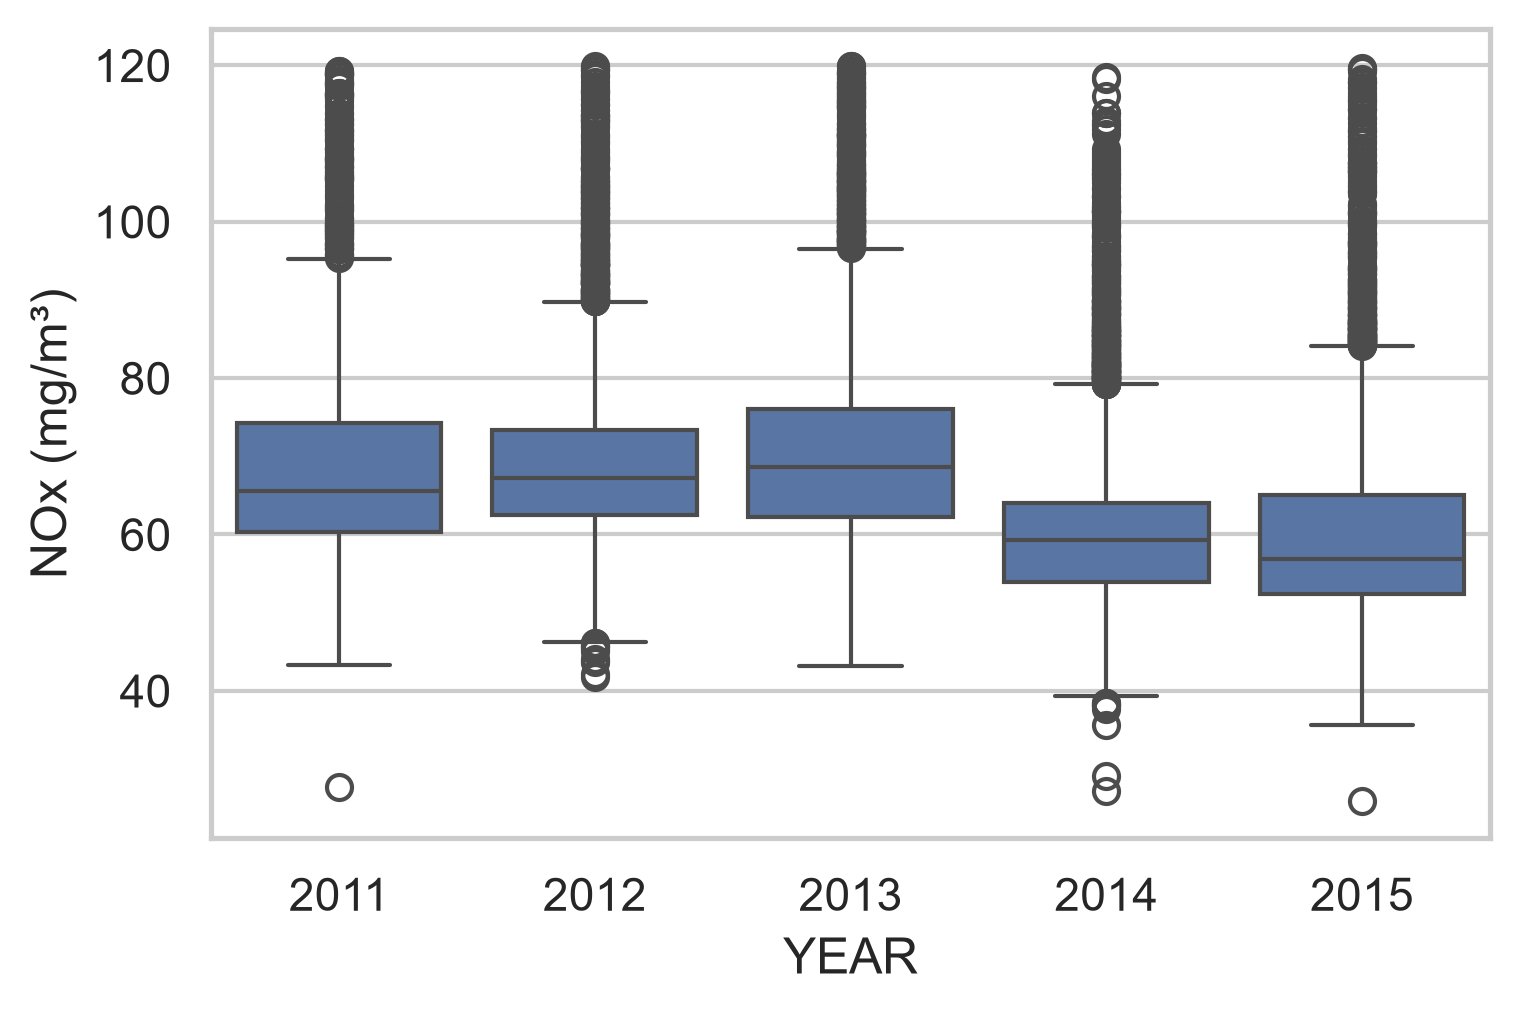
\includegraphics[keepaspectratio]{notebooks/04-testing_files/figure-pdf/cell-5-output-1.png}}

The box plots show the distribution of NOx per year. Before testing,
look at the size of the differences between the medians compared with
the spread within each year -- this is what the tests will formalise.

\begin{Shaded}
\begin{Highlighting}[]
\NormalTok{groups }\OperatorTok{=}\NormalTok{ [g[}\StringTok{"NOX"}\NormalTok{].values }\ControlFlowTok{for}\NormalTok{ \_, g }\KeywordTok{in}\NormalTok{ gt.groupby(}\StringTok{"YEAR"}\NormalTok{)]}
\BuiltInTok{print}\NormalTok{(}\StringTok{"ANOVA:         "}\NormalTok{, stats.f\_oneway(}\OperatorTok{*}\NormalTok{groups))}
\BuiltInTok{print}\NormalTok{(}\StringTok{"Kruskal{-}Wallis:"}\NormalTok{, stats.kruskal(}\OperatorTok{*}\NormalTok{groups))}

\NormalTok{a, b }\OperatorTok{=}\NormalTok{ gt.loc[gt.YEAR }\OperatorTok{==} \DecValTok{2011}\NormalTok{, }\StringTok{"NOX"}\NormalTok{], gt.loc[gt.YEAR }\OperatorTok{==} \DecValTok{2015}\NormalTok{, }\StringTok{"NOX"}\NormalTok{]}
\NormalTok{res }\OperatorTok{=}\NormalTok{ stats.ttest\_ind(a, b, equal\_var}\OperatorTok{=}\VariableTok{False}\NormalTok{)}
\NormalTok{ci }\OperatorTok{=}\NormalTok{ res.confidence\_interval(}\FloatTok{0.95}\NormalTok{)}
\NormalTok{cohens\_d }\OperatorTok{=}\NormalTok{ (a.mean() }\OperatorTok{{-}}\NormalTok{ b.mean()) }\OperatorTok{/}\NormalTok{ np.sqrt((a.var() }\OperatorTok{+}\NormalTok{ b.var()) }\OperatorTok{/} \DecValTok{2}\NormalTok{)}
\BuiltInTok{print}\NormalTok{(}\SpecialStringTok{f"Welch t{-}test 2011 vs 2015: p = }\SpecialCharTok{\{}\NormalTok{res}\SpecialCharTok{.}\NormalTok{pvalue}\SpecialCharTok{:.2e\}}\SpecialStringTok{"}\NormalTok{)}
\BuiltInTok{print}\NormalTok{(}\SpecialStringTok{f"difference = }\SpecialCharTok{\{}\NormalTok{a}\SpecialCharTok{.}\NormalTok{mean() }\OperatorTok{{-}}\NormalTok{ b}\SpecialCharTok{.}\NormalTok{mean()}\SpecialCharTok{:.1f\}}\SpecialStringTok{ mg/m³, 95 \% CI [}\SpecialCharTok{\{}\NormalTok{ci}\SpecialCharTok{.}\NormalTok{low}\SpecialCharTok{:.1f\}}\SpecialStringTok{, }\SpecialCharTok{\{}\NormalTok{ci}\SpecialCharTok{.}\NormalTok{high}\SpecialCharTok{:.1f\}}\SpecialStringTok{], Cohen\textquotesingle{}s d = }\SpecialCharTok{\{}\NormalTok{cohens\_d}\SpecialCharTok{:.2f\}}\SpecialStringTok{"}\NormalTok{)}
\end{Highlighting}
\end{Shaded}

\begin{verbatim}
ANOVA:          F_onewayResult(statistic=np.float64(1495.9585853305857), pvalue=np.float64(0.0))
Kruskal-Wallis: KruskalResult(statistic=np.float64(6795.540640131331), pvalue=np.float64(0.0))
Welch t-test 2011 vs 2015: p = 0.00e+00
difference = 7.7 mg/m³, 95 % CI [7.3, 8.0], Cohen's d = 0.70
\end{verbatim}

\textbf{Discussion.} With several thousand hourly values per year, the
p-values are astronomically small -- any systematic difference between
years is detected. The informative numbers are the difference in mg/m³
with its confidence interval and Cohen's d.~Whether the change matters
depends on the distance to the emission limit and on the cause.

And here an engineering caution is needed: the hourly values are
\textbf{not independent} -- consecutive hours are strongly correlated,
so the effective sample size is much smaller than the number of rows,
and the p-values are too optimistic. Moreover, differences between years
can be caused by different ambient conditions (a hot year), different
load profiles or maintenance work. A test can establish \emph{that} the
years differ, not \emph{why}. To attribute the change to a cause we
would need a model that accounts for these influences (Chapter 5).

\section{Live coding: product variant and machine
failures}\label{live-coding-product-variant-and-machine-failures}

The AI4I dataset is a synthetic dataset modelled on a real milling
process. Each of the 10,000 records belongs to a product of quality
variant L (low, 50 \% of products), M (medium, 30 \%) or H (high, 20
\%). Is the failure rate independent of the variant? Both variables are
categorical, so we use the chi-squared test.

\begin{Shaded}
\begin{Highlighting}[]
\ImportTok{from}\NormalTok{ ucimlrepo }\ImportTok{import}\NormalTok{ fetch\_ucirepo}

\NormalTok{ai4i }\OperatorTok{=}\NormalTok{ fetch\_ucirepo(}\BuiltInTok{id}\OperatorTok{=}\DecValTok{601}\NormalTok{).data.original}
\NormalTok{table }\OperatorTok{=}\NormalTok{ pd.crosstab(ai4i[}\StringTok{"Type"}\NormalTok{], ai4i[}\StringTok{"Machine failure"}\NormalTok{])}
\NormalTok{chi2, p, dof, expected }\OperatorTok{=}\NormalTok{ stats.chi2\_contingency(table)}
\BuiltInTok{print}\NormalTok{(table, }\SpecialStringTok{f"}\CharTok{\textbackslash{}n}\SpecialStringTok{chi2 = }\SpecialCharTok{\{}\NormalTok{chi2}\SpecialCharTok{:.2f\}}\SpecialStringTok{, dof = }\SpecialCharTok{\{}\NormalTok{dof}\SpecialCharTok{\}}\SpecialStringTok{, p = }\SpecialCharTok{\{}\NormalTok{p}\SpecialCharTok{:.3f\}}\SpecialStringTok{"}\NormalTok{)}
\NormalTok{(table[}\DecValTok{1}\NormalTok{] }\OperatorTok{/}\NormalTok{ table.}\BuiltInTok{sum}\NormalTok{(axis}\OperatorTok{=}\DecValTok{1}\NormalTok{)).rename(}\StringTok{"failure rate"}\NormalTok{).}\BuiltInTok{round}\NormalTok{(}\DecValTok{4}\NormalTok{)}
\end{Highlighting}
\end{Shaded}

\begin{verbatim}
Machine failure     0    1
Type                      
H                 982   21
L                5765  235
M                2914   83 
chi2 = 13.75, dof = 2, p = 0.001
\end{verbatim}

\begin{verbatim}
Type
H    0.0209
L    0.0392
M    0.0277
Name: failure rate, dtype: float64
\end{verbatim}

\textbf{Discussion.} Compare the failure rates per variant and the
p-value. The chi-squared test needs sufficiently large expected counts
(rule of thumb: at least 5 in every cell) -- check \texttt{expected}.
Even if the test is significant, ask whether the difference in failure
rates is relevant, and whether the variants differ in other respects
(e.g.~tool wear or load) that could explain it.

\section{How many measurements do we
need?}\label{how-many-measurements-do-we-need}

Planning comes before testing. If a difference of \(\delta\) is
relevant, how many samples are needed to detect it with a power of, say,
80 \%? For the two-sample t-test, the required number per group is
approximately

\[n \approx \frac{2\,(z_{1-\alpha/2} + z_{1-\beta})^2}{d^2}, \qquad d = \delta/\sigma,\]

where \(\delta\) is the smallest relevant difference, \(\sigma\) the
standard deviation and \(z_q\) the \(q\)-quantile of the standard normal
distribution. This gives about \(16/d^2\) for \(\alpha = 0.05\) and
power 0.8. Halving the detectable effect requires four times as many
samples.

\begin{Shaded}
\begin{Highlighting}[]
\ImportTok{from}\NormalTok{ statsmodels.stats.power }\ImportTok{import}\NormalTok{ TTestIndPower}

\NormalTok{power\_analysis }\OperatorTok{=}\NormalTok{ TTestIndPower()}
\ControlFlowTok{for}\NormalTok{ d }\KeywordTok{in}\NormalTok{ [}\FloatTok{0.2}\NormalTok{, }\FloatTok{0.5}\NormalTok{, }\FloatTok{0.8}\NormalTok{]:}
\NormalTok{    n }\OperatorTok{=}\NormalTok{ power\_analysis.solve\_power(effect\_size}\OperatorTok{=}\NormalTok{d, alpha}\OperatorTok{=}\FloatTok{0.05}\NormalTok{, power}\OperatorTok{=}\FloatTok{0.8}\NormalTok{)}
    \BuiltInTok{print}\NormalTok{(}\SpecialStringTok{f"d = }\SpecialCharTok{\{}\NormalTok{d}\SpecialCharTok{\}}\SpecialStringTok{: n = }\SpecialCharTok{\{}\NormalTok{np}\SpecialCharTok{.}\NormalTok{ceil(n)}\SpecialCharTok{:.0f\}}\SpecialStringTok{ per group"}\NormalTok{)}
\end{Highlighting}
\end{Shaded}

\begin{verbatim}
d = 0.2: n = 394 per group
d = 0.5: n = 64 per group
d = 0.8: n = 26 per group
\end{verbatim}

\section{Back to the decision}\label{back-to-the-decision-3}

The contract requires two things: the reduction must be
\emph{demonstrable} (larger than random variation) and \emph{relevant}
(at least 5 \% of the 2011 mean). A small p-value only covers the first
part. We therefore look at the confidence interval of the difference:
the bonus is justified only if the whole interval lies above the
relevance threshold.

\begin{Shaded}
\begin{Highlighting}[]
\NormalTok{nox\_2011 }\OperatorTok{=}\NormalTok{ gt.loc[gt.YEAR }\OperatorTok{==} \DecValTok{2011}\NormalTok{, }\StringTok{"NOX"}\NormalTok{]}
\NormalTok{nox\_2015 }\OperatorTok{=}\NormalTok{ gt.loc[gt.YEAR }\OperatorTok{==} \DecValTok{2015}\NormalTok{, }\StringTok{"NOX"}\NormalTok{]}
\NormalTok{res\_bonus }\OperatorTok{=}\NormalTok{ stats.ttest\_ind(nox\_2011, nox\_2015, equal\_var}\OperatorTok{=}\VariableTok{False}\NormalTok{)}
\NormalTok{ci\_red }\OperatorTok{=}\NormalTok{ res\_bonus.confidence\_interval(}\FloatTok{0.95}\NormalTok{)              }\CommentTok{\# CI of mean(2011) {-} mean(2015)}
\NormalTok{threshold }\OperatorTok{=} \FloatTok{0.05} \OperatorTok{*}\NormalTok{ nox\_2011.mean()}
\BuiltInTok{print}\NormalTok{(}\SpecialStringTok{f"Reduction 2011 {-}\textgreater{} 2015: }\SpecialCharTok{\{}\NormalTok{nox\_2011}\SpecialCharTok{.}\NormalTok{mean() }\OperatorTok{{-}}\NormalTok{ nox\_2015}\SpecialCharTok{.}\NormalTok{mean()}\SpecialCharTok{:.1f\}}\SpecialStringTok{ mg/m³, "}
      \SpecialStringTok{f"95 \% CI [}\SpecialCharTok{\{}\NormalTok{ci\_red}\SpecialCharTok{.}\NormalTok{low}\SpecialCharTok{:.1f\}}\SpecialStringTok{, }\SpecialCharTok{\{}\NormalTok{ci\_red}\SpecialCharTok{.}\NormalTok{high}\SpecialCharTok{:.1f\}}\SpecialStringTok{], relevance threshold }\SpecialCharTok{\{}\NormalTok{threshold}\SpecialCharTok{:.1f\}}\SpecialStringTok{ mg/m³"}\NormalTok{)}
\ControlFlowTok{if}\NormalTok{ ci\_red.low }\OperatorTok{\textgreater{}}\NormalTok{ threshold:}
    \BuiltInTok{print}\NormalTok{(}\StringTok{"Decision: claim confirmed – the reduction is demonstrable and relevant."}\NormalTok{)}
\ControlFlowTok{elif}\NormalTok{ ci\_red.low }\OperatorTok{\textgreater{}} \DecValTok{0}\NormalTok{:}
    \BuiltInTok{print}\NormalTok{(}\StringTok{"Decision: reduction demonstrable, but not demonstrably relevant – no bonus under the contract."}\NormalTok{)}
\ControlFlowTok{else}\NormalTok{:}
    \BuiltInTok{print}\NormalTok{(}\StringTok{"Decision: no demonstrable reduction – claim rejected."}\NormalTok{)}
\end{Highlighting}
\end{Shaded}

\begin{verbatim}
Reduction 2011 -> 2015: 7.7 mg/m³, 95 % CI [7.3, 8.0], relevance threshold 3.4 mg/m³
Decision: claim confirmed – the reduction is demonstrable and relevant.
\end{verbatim}

Two further points belong in the review. The hourly values are
autocorrelated, so the true uncertainty is larger than the interval
suggests -- a borderline case should be decided against the claim. And
even a confirmed reduction does not prove that the consultant
\emph{caused} it: different weather, load profiles or maintenance could
have the same effect. A fair contract would have specified how such
influences are accounted for -- a lesson for the next one.

\begin{tcolorbox}[enhanced jigsaw, colframe=quarto-callout-important-color-frame, toprule=.15mm, rightrule=.15mm, title=\textcolor{quarto-callout-important-color}{\faExclamation}\hspace{0.5em}{Key takeaways}, colbacktitle=quarto-callout-important-color!10!white, left=2mm, titlerule=0mm, bottomtitle=1mm, toptitle=1mm, opacityback=0, bottomrule=.15mm, breakable, arc=.35mm, opacitybacktitle=0.6, colback=white, coltitle=black, leftrule=.75mm]

\begin{itemize}
\tightlist
\item
  A test checks whether data are compatible with ``no effect''; the
  p-value is a probability \emph{under} \(H_0\), not \emph{of} \(H_0\).
\item
  Report effect sizes and confidence intervals, not just p-values; judge
  relevance in physical units.
\item
  Large samples make tiny effects significant; small samples miss
  relevant effects -- plan the sample size.
\item
  Many tests produce false alarms; correct (Bonferroni, Holm) and plan
  comparisons in advance.
\item
  Tests assume independent observations -- time series data violate
  this.
\end{itemize}

\end{tcolorbox}

\section{Exercises}\label{exercises-3}

\begin{enumerate}
\def\labelenumi{\arabic{enumi}.}
\tightlist
\item
  Check the normality assumption for NOx per year with QQ plots. Does a
  violation matter for the ANOVA with these sample sizes?
\item
  Draw a random sample of 30 hourly values per year and repeat the ANOVA
  and the 2011 vs.~2015 t-test. What changes and why? Repeat the
  sampling a few times.
\item
  Run pairwise Welch t-tests between all years. How many comparisons are
  there? Apply a Bonferroni and a Holm correction.
\item
  Formulate an engineering conclusion from the NOx analysis in two or
  three sentences -- for a plant manager, not for a statistician.
\item
  A new coating is supposed to reduce the wear of a tool by 10 µm. From
  previous tests the standard deviation of the wear is 25 µm. How many
  tools must be tested per variant to detect the improvement with 80 \%
  power (\(\alpha = 0.05\))?
\end{enumerate}

\subsection{Solutions}\label{solutions-3}

\begin{tcolorbox}[enhanced jigsaw, colframe=quarto-callout-caution-color-frame, toprule=.15mm, rightrule=.15mm, title=\textcolor{quarto-callout-caution-color}{\faFire}\hspace{0.5em}{Solution to Exercise 1}, colbacktitle=quarto-callout-caution-color!10!white, left=2mm, titlerule=0mm, bottomtitle=1mm, toptitle=1mm, opacityback=0, bottomrule=.15mm, breakable, arc=.35mm, opacitybacktitle=0.6, colback=white, coltitle=black, leftrule=.75mm]

\begin{Shaded}
\begin{Highlighting}[]
\NormalTok{years }\OperatorTok{=} \BuiltInTok{sorted}\NormalTok{(gt[}\StringTok{"YEAR"}\NormalTok{].unique())}
\NormalTok{fig, axes }\OperatorTok{=}\NormalTok{ plt.subplots(}\DecValTok{1}\NormalTok{, }\BuiltInTok{len}\NormalTok{(years), figsize}\OperatorTok{=}\NormalTok{(}\DecValTok{16}\NormalTok{, }\FloatTok{3.5}\NormalTok{))}
\ControlFlowTok{for}\NormalTok{ ax, yr }\KeywordTok{in} \BuiltInTok{zip}\NormalTok{(axes, years):}
\NormalTok{    stats.probplot(gt.loc[gt.YEAR }\OperatorTok{==}\NormalTok{ yr, }\StringTok{"NOX"}\NormalTok{], dist}\OperatorTok{=}\StringTok{"norm"}\NormalTok{, plot}\OperatorTok{=}\NormalTok{ax)}
\NormalTok{    ax.set\_title(}\BuiltInTok{str}\NormalTok{(yr))}
\NormalTok{plt.tight\_layout()}\OperatorTok{;}\NormalTok{ plt.show()}
\end{Highlighting}
\end{Shaded}

\pandocbounded{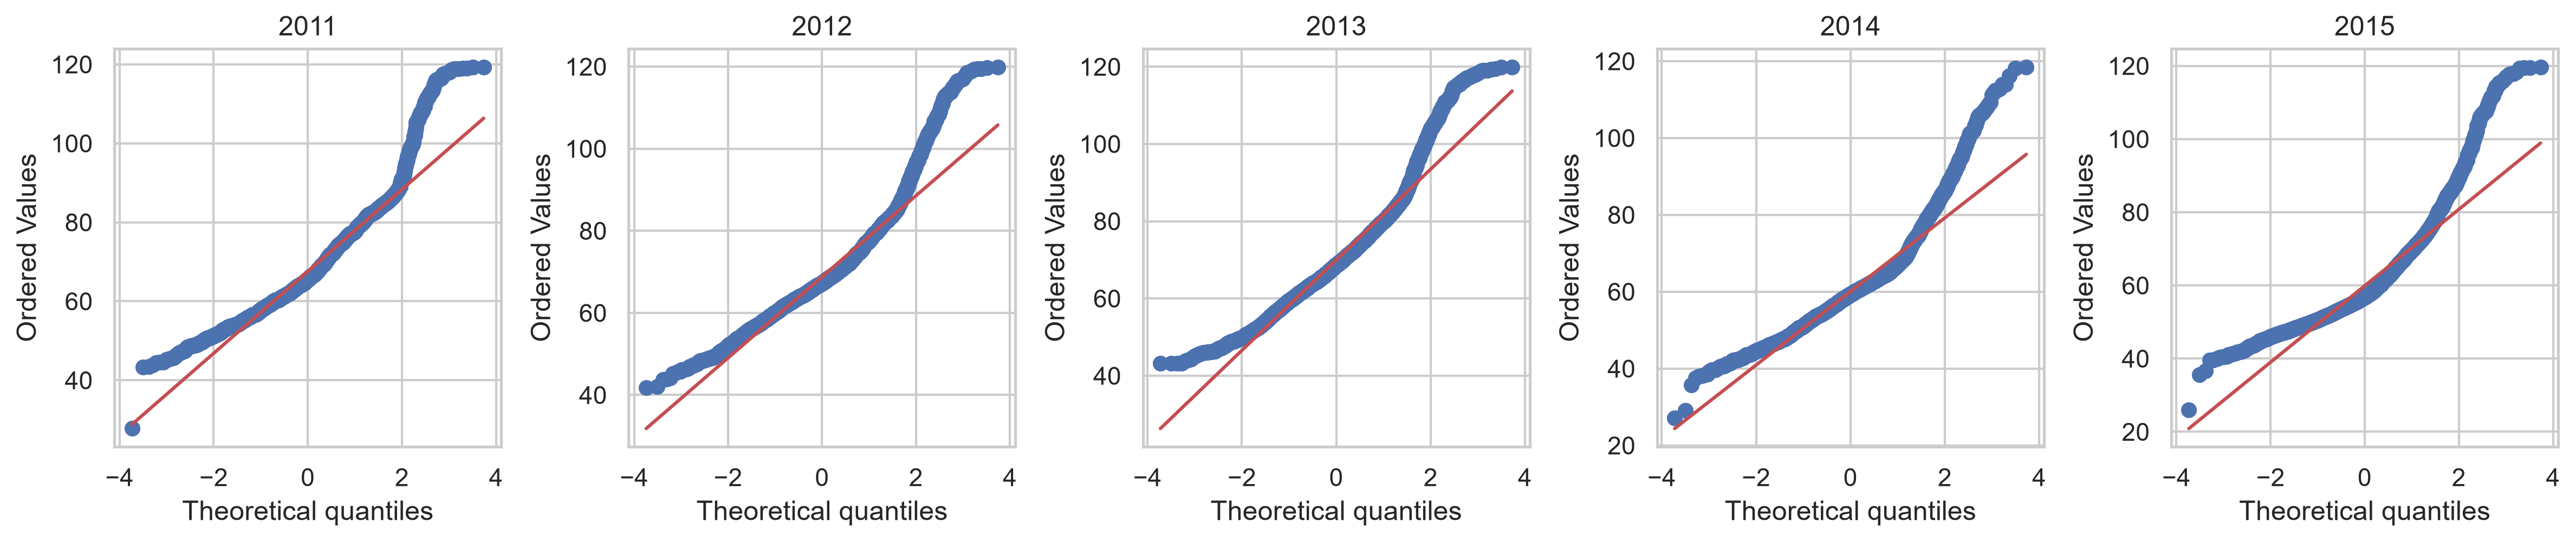
\includegraphics[keepaspectratio]{notebooks/04-testing_files/figure-pdf/cell-10-output-1.png}}

Deviations from the straight line at the ends indicate heavier or
lighter tails than the normal distribution, curvature indicates
skewness. With thousands of observations per group, the central limit
theorem makes the group \emph{means} approximately normal, so the ANOVA
is robust against moderate non-normality. More critical are the unequal
variances between years and above all the dependence of consecutive
hourly values. The Kruskal--Wallis test, which does not assume
normality, serves as a cross-check.

\end{tcolorbox}

\begin{tcolorbox}[enhanced jigsaw, colframe=quarto-callout-caution-color-frame, toprule=.15mm, rightrule=.15mm, title=\textcolor{quarto-callout-caution-color}{\faFire}\hspace{0.5em}{Solution to Exercise 2}, colbacktitle=quarto-callout-caution-color!10!white, left=2mm, titlerule=0mm, bottomtitle=1mm, toptitle=1mm, opacityback=0, bottomrule=.15mm, breakable, arc=.35mm, opacitybacktitle=0.6, colback=white, coltitle=black, leftrule=.75mm]

\begin{Shaded}
\begin{Highlighting}[]
\ControlFlowTok{for}\NormalTok{ seed }\KeywordTok{in} \BuiltInTok{range}\NormalTok{(}\DecValTok{3}\NormalTok{):}
\NormalTok{    small }\OperatorTok{=}\NormalTok{ gt.groupby(}\StringTok{"YEAR"}\NormalTok{, group\_keys}\OperatorTok{=}\VariableTok{False}\NormalTok{).sample(}\DecValTok{30}\NormalTok{, random\_state}\OperatorTok{=}\NormalTok{seed)}
\NormalTok{    groups\_s }\OperatorTok{=}\NormalTok{ [g[}\StringTok{"NOX"}\NormalTok{].values }\ControlFlowTok{for}\NormalTok{ \_, g }\KeywordTok{in}\NormalTok{ small.groupby(}\StringTok{"YEAR"}\NormalTok{)]}
\NormalTok{    a\_s }\OperatorTok{=}\NormalTok{ small.loc[small.YEAR }\OperatorTok{==} \DecValTok{2011}\NormalTok{, }\StringTok{"NOX"}\NormalTok{]}\OperatorTok{;}\NormalTok{ b\_s }\OperatorTok{=}\NormalTok{ small.loc[small.YEAR }\OperatorTok{==} \DecValTok{2015}\NormalTok{, }\StringTok{"NOX"}\NormalTok{]}
    \BuiltInTok{print}\NormalTok{(}\SpecialStringTok{f"seed }\SpecialCharTok{\{}\NormalTok{seed}\SpecialCharTok{\}}\SpecialStringTok{: ANOVA p = }\SpecialCharTok{\{}\NormalTok{stats}\SpecialCharTok{.}\NormalTok{f\_oneway(}\OperatorTok{*}\NormalTok{groups\_s)}\SpecialCharTok{.}\NormalTok{pvalue}\SpecialCharTok{:.3g\}}\SpecialStringTok{, "}
          \SpecialStringTok{f"t{-}test p = }\SpecialCharTok{\{}\NormalTok{stats}\SpecialCharTok{.}\NormalTok{ttest\_ind(a\_s, b\_s, equal\_var}\OperatorTok{=}\VariableTok{False}\NormalTok{)}\SpecialCharTok{.}\NormalTok{pvalue}\SpecialCharTok{:.3g\}}\SpecialStringTok{, "}
          \SpecialStringTok{f"difference = }\SpecialCharTok{\{}\NormalTok{a\_s}\SpecialCharTok{.}\NormalTok{mean() }\OperatorTok{{-}}\NormalTok{ b\_s}\SpecialCharTok{.}\NormalTok{mean()}\SpecialCharTok{:.1f\}}\SpecialStringTok{ mg/m³"}\NormalTok{)}
\end{Highlighting}
\end{Shaded}

\begin{verbatim}
seed 0: ANOVA p = 0.000462, t-test p = 0.203, difference = 4.5 mg/m³
seed 1: ANOVA p = 5.7e-07, t-test p = 0.000116, difference = 8.8 mg/m³
seed 2: ANOVA p = 7.32e-06, t-test p = 0.0237, difference = 7.0 mg/m³
\end{verbatim}

The estimated differences stay of similar size, but the p-values are
much larger and vary from sample to sample: with 30 values per year, the
standard error is roughly \(\sqrt{7000/30} \approx 15\) times larger.
Small differences that were ``highly significant'' with all data may no
longer be detectable. The effect did not change -- only the power of the
test.

\end{tcolorbox}

\begin{tcolorbox}[enhanced jigsaw, colframe=quarto-callout-caution-color-frame, toprule=.15mm, rightrule=.15mm, title=\textcolor{quarto-callout-caution-color}{\faFire}\hspace{0.5em}{Solution to Exercise 3}, colbacktitle=quarto-callout-caution-color!10!white, left=2mm, titlerule=0mm, bottomtitle=1mm, toptitle=1mm, opacityback=0, bottomrule=.15mm, breakable, arc=.35mm, opacitybacktitle=0.6, colback=white, coltitle=black, leftrule=.75mm]

\begin{Shaded}
\begin{Highlighting}[]
\ImportTok{import}\NormalTok{ itertools}
\ImportTok{from}\NormalTok{ statsmodels.stats.multitest }\ImportTok{import}\NormalTok{ multipletests}

\NormalTok{pairs, pvals }\OperatorTok{=}\NormalTok{ [], []}
\ControlFlowTok{for}\NormalTok{ y1, y2 }\KeywordTok{in}\NormalTok{ itertools.combinations(years, }\DecValTok{2}\NormalTok{):}
\NormalTok{    pairs.append(}\SpecialStringTok{f"}\SpecialCharTok{\{}\NormalTok{y1}\SpecialCharTok{\}}\SpecialStringTok{{-}}\SpecialCharTok{\{}\NormalTok{y2}\SpecialCharTok{\}}\SpecialStringTok{"}\NormalTok{)}
\NormalTok{    pvals.append(stats.ttest\_ind(gt.loc[gt.YEAR }\OperatorTok{==}\NormalTok{ y1, }\StringTok{"NOX"}\NormalTok{], gt.loc[gt.YEAR }\OperatorTok{==}\NormalTok{ y2, }\StringTok{"NOX"}\NormalTok{],}
\NormalTok{                                 equal\_var}\OperatorTok{=}\VariableTok{False}\NormalTok{).pvalue)}
\NormalTok{result }\OperatorTok{=}\NormalTok{ pd.DataFrame(\{}\StringTok{"p"}\NormalTok{: pvals,}
                       \StringTok{"Bonferroni"}\NormalTok{: multipletests(pvals, method}\OperatorTok{=}\StringTok{"bonferroni"}\NormalTok{)[}\DecValTok{1}\NormalTok{],}
                       \StringTok{"Holm"}\NormalTok{: multipletests(pvals, method}\OperatorTok{=}\StringTok{"holm"}\NormalTok{)[}\DecValTok{1}\NormalTok{]\}, index}\OperatorTok{=}\NormalTok{pairs)}
\NormalTok{result.style.}\BuiltInTok{format}\NormalTok{(}\StringTok{"}\SpecialCharTok{\{:.2e\}}\StringTok{"}\NormalTok{)}
\end{Highlighting}
\end{Shaded}

\begin{longtable}[]{@{}llll@{}}
\caption{}\label{T_e0b44}\tabularnewline
\toprule\noalign{}
~ & p & Bonferroni & Holm \\
\midrule\noalign{}
\endfirsthead
\toprule\noalign{}
~ & p & Bonferroni & Holm \\
\midrule\noalign{}
\endhead
\bottomrule\noalign{}
\endlastfoot
2011-2012 & 1.18e-12 & 1.18e-11 & 3.55e-12 \\
2011-2013 & 1.01e-37 & 1.01e-36 & 4.06e-37 \\
2011-2014 & 0.00e+00 & 0.00e+00 & 0.00e+00 \\
2011-2015 & 0.00e+00 & 0.00e+00 & 0.00e+00 \\
2012-2013 & 3.97e-11 & 3.97e-10 & 7.94e-11 \\
2012-2014 & 0.00e+00 & 0.00e+00 & 0.00e+00 \\
2012-2015 & 0.00e+00 & 0.00e+00 & 0.00e+00 \\
2013-2014 & 0.00e+00 & 0.00e+00 & 0.00e+00 \\
2013-2015 & 0.00e+00 & 0.00e+00 & 0.00e+00 \\
2014-2015 & 3.14e-01 & 1.00e+00 & 3.14e-01 \\
\end{longtable}

With 5 years there are \(\binom{5}{2} = 10\) comparisons. Bonferroni
multiplies each p-value by 10 (capped at 1); Holm multiplies the
smallest by 10, the next by 9 and so on, and is therefore less
conservative. With these large samples most comparisons remain
significant even after correction -- the correction matters most when
p-values are close to \(\alpha\).

\end{tcolorbox}

\begin{tcolorbox}[enhanced jigsaw, colframe=quarto-callout-caution-color-frame, toprule=.15mm, rightrule=.15mm, title=\textcolor{quarto-callout-caution-color}{\faFire}\hspace{0.5em}{Solution to Exercise 4}, colbacktitle=quarto-callout-caution-color!10!white, left=2mm, titlerule=0mm, bottomtitle=1mm, toptitle=1mm, opacityback=0, bottomrule=.15mm, breakable, arc=.35mm, opacitybacktitle=0.6, colback=white, coltitle=black, leftrule=.75mm]

A good answer states the size of the change in physical units, relates
it to a meaningful reference and names the limits of the analysis, for
example: ``The mean NOx emission in 2015 was X mg/m³ lower (higher) than
in 2011, a change of about Y \% of the typical level. This difference is
clearly larger than random variation. The data alone do not show whether
the change was caused by maintenance, different operation or different
weather; to find out, we should model the emissions as a function of
load and ambient conditions.'' (Insert X and Y from your results.) Avoid
statistical jargon such as ``p \textless{} 0.001'' without explanation.

\end{tcolorbox}

\begin{tcolorbox}[enhanced jigsaw, colframe=quarto-callout-caution-color-frame, toprule=.15mm, rightrule=.15mm, title=\textcolor{quarto-callout-caution-color}{\faFire}\hspace{0.5em}{Solution to Exercise 5}, colbacktitle=quarto-callout-caution-color!10!white, left=2mm, titlerule=0mm, bottomtitle=1mm, toptitle=1mm, opacityback=0, bottomrule=.15mm, breakable, arc=.35mm, opacitybacktitle=0.6, colback=white, coltitle=black, leftrule=.75mm]

\begin{Shaded}
\begin{Highlighting}[]
\NormalTok{d }\OperatorTok{=} \DecValTok{10} \OperatorTok{/} \DecValTok{25}
\NormalTok{n }\OperatorTok{=}\NormalTok{ TTestIndPower().solve\_power(effect\_size}\OperatorTok{=}\NormalTok{d, alpha}\OperatorTok{=}\FloatTok{0.05}\NormalTok{, power}\OperatorTok{=}\FloatTok{0.8}\NormalTok{)}
\BuiltInTok{print}\NormalTok{(}\SpecialStringTok{f"d = }\SpecialCharTok{\{}\NormalTok{d}\SpecialCharTok{\}}\SpecialStringTok{, n = }\SpecialCharTok{\{}\NormalTok{np}\SpecialCharTok{.}\NormalTok{ceil(n)}\SpecialCharTok{:.0f\}}\SpecialStringTok{ tools per variant (rule of thumb 16/d² = }\SpecialCharTok{\{}\DecValTok{16} \OperatorTok{/}\NormalTok{ d}\OperatorTok{**}\DecValTok{2}\SpecialCharTok{:.0f\}}\SpecialStringTok{)"}\NormalTok{)}
\end{Highlighting}
\end{Shaded}

\begin{verbatim}
d = 0.4, n = 100 tools per variant (rule of thumb 16/d² = 100)
\end{verbatim}

The effect size is \(d = 10/25 = 0.4\), which requires about 100 tools
per variant. If that is too expensive, options are: reduce the noise
(more homogeneous test conditions, paired design with both coatings on
the same machine), accept a lower power, or test for a larger minimum
effect.

\end{tcolorbox}

\chapter{Linear and Nonlinear
Regression}\label{linear-and-nonlinear-regression}

Regression is the workhorse of engineering data analysis. Calibration
curves, empirical material laws, characteristic maps of engines and
process models are all regression models: they describe how a quantity
of interest -- the \emph{response} -- depends on one or more influencing
quantities -- the \emph{inputs}, \emph{factors} or \emph{features}. A
regression model can be used to \textbf{understand} a process (which
factors matter, how strongly?) and to \textbf{predict} the response for
new input values.

This chapter starts with the multiple linear regression model, its
estimation by least squares and the statistical tools to interpret and
check it. We then fit nonlinear models with physical meaning, which are
common in engineering. An extension section shows how designed
experiments make sure that the data actually contain the information we
need.

\textbf{Scenario: releasing a precast element}

A precast concrete plant wants to use a new, cheaper mix: 350 kg cement
and 180 kg water per m³, 5 kg superplasticizer, no slag or fly ash. The
elements require a compressive strength of 35 MPa before they may be
loaded. No test specimens of the new mix exist yet, and the production
manager asks: ``Can we promise the customer 35 MPa after 28 days -- and
if not, when?''

\textbf{Your decision:} Approve the mix for the 28-day delivery promise
-- or name a later date?

\textbf{Learning goals.} After this chapter you can

\begin{itemize}
\tightlist
\item
  fit and interpret multiple linear regression models with statsmodels,
\item
  explain least squares, coefficient standard errors, R² and the
  difference between confidence and prediction intervals,
\item
  check model assumptions with residual analysis and recognise
  collinearity,
\item
  include transformations and interaction terms,
\item
  fit nonlinear physical or empirical models with
  \texttt{scipy.optimize.curve\_fit} and quantify parameter uncertainty,
\item
  (extension) plan a full factorial experiment and estimate main effects
  and interactions.
\end{itemize}

\textbf{Datasets in this chapter}

\begin{itemize}
\tightlist
\item
  \href{https://archive.ics.uci.edu/dataset/165/concrete+compressive+strength}{Concrete
  Compressive Strength (UCI)}
\end{itemize}

\section{The linear model}\label{the-linear-model}

\begin{tcolorbox}[enhanced jigsaw, colframe=quarto-callout-note-color-frame, toprule=.15mm, rightrule=.15mm, title=\textcolor{quarto-callout-note-color}{\faInfo}\hspace{0.5em}{Definition: Multiple linear regression}, colbacktitle=quarto-callout-note-color!10!white, left=2mm, titlerule=0mm, bottomtitle=1mm, toptitle=1mm, opacityback=0, bottomrule=.15mm, breakable, arc=.35mm, opacitybacktitle=0.6, colback=white, coltitle=black, leftrule=.75mm]

The response \(y\) is modelled as a linear function of \(p\) inputs plus
a random error:
\[y_i = \beta_0 + \beta_1 x_{i1} + \dots + \beta_p x_{ip} + \varepsilon_i, \qquad \varepsilon_i \sim N(0, \sigma^2) \text{ independent}.\]
In matrix form, \(y = X\beta + \varepsilon\), where the design matrix
\(X\) has a first column of ones for the intercept.

\end{tcolorbox}

``Linear'' refers to the \textbf{parameters}, not to the inputs. Models
like \(y = \beta_0 + \beta_1 \ln x + \beta_2 x^2\) or
\(y = \beta_0 + \beta_1 x_1 x_2\) are linear models, because they are
linear in \(\beta\). This makes the linear model much more flexible than
its name suggests.

\subsection{Estimation by least
squares}\label{estimation-by-least-squares}

The coefficients are chosen to minimise the sum of squared residuals
\(\sum_i (y_i - \hat y_i)^2\). Setting the derivatives to zero gives the
\textbf{normal equations} and their solution:

\begin{tcolorbox}[enhanced jigsaw, colframe=quarto-callout-important-color-frame, toprule=.15mm, rightrule=.15mm, title=\textcolor{quarto-callout-important-color}{\faExclamation}\hspace{0.5em}{Least squares estimate}, colbacktitle=quarto-callout-important-color!10!white, left=2mm, titlerule=0mm, bottomtitle=1mm, toptitle=1mm, opacityback=0, bottomrule=.15mm, breakable, arc=.35mm, opacitybacktitle=0.6, colback=white, coltitle=black, leftrule=.75mm]

\[\hat\beta = (X^\top X)^{-1} X^\top y, \qquad \widehat{\text{Cov}}(\hat\beta) = \hat\sigma^2 (X^\top X)^{-1}, \qquad \hat\sigma^2 = \frac{1}{n - p - 1}\sum_i (y_i - \hat y_i)^2.\]
The square roots of the diagonal of \(\widehat{\text{Cov}}(\hat\beta)\)
are the \textbf{standard errors} of the coefficients.

\end{tcolorbox}

(Numerically, software never inverts \(X^\top X\) explicitly but uses a
QR or SVD decomposition -- more stable, same result.)

\subsection{Interpreting the output}\label{interpreting-the-output}

\begin{itemize}
\tightlist
\item
  \textbf{Coefficient \(\hat\beta_j\):} expected change of \(y\) when
  \(x_j\) increases by one unit \emph{and all other inputs stay
  constant}. The last part is crucial -- and often unrealistic when
  inputs are correlated.
\item
  \textbf{Standard error, t-value, p-value:} test of
  \(H_0: \beta_j = 0\) given the other inputs in the model; the 95 \%
  confidence interval is
  \(\hat\beta_j \pm t_{0.975}\,\text{SE}(\hat\beta_j)\).
\item
  \textbf{Coefficient of determination}
  \(R^2 = 1 - \frac{\sum (y_i - \hat y_i)^2}{\sum (y_i - \bar y)^2}\):
  share of the variance of \(y\) explained by the model. It never
  decreases when inputs are added; the \textbf{adjusted \(R^2\)}
  penalises additional inputs.
\end{itemize}

\begin{tcolorbox}[enhanced jigsaw, colframe=quarto-callout-warning-color-frame, toprule=.15mm, rightrule=.15mm, title=\textcolor{quarto-callout-warning-color}{\faExclamationTriangle}\hspace{0.5em}{Pitfall: R² measures fit, not validity}, colbacktitle=quarto-callout-warning-color!10!white, left=2mm, titlerule=0mm, bottomtitle=1mm, toptitle=1mm, opacityback=0, bottomrule=.15mm, breakable, arc=.35mm, opacitybacktitle=0.6, colback=white, coltitle=black, leftrule=.75mm]

A high \(R^2\) does not mean that the model is correct, that it predicts
well on new data or that the relationships are causal. Conversely, a low
\(R^2\) can be perfectly acceptable if the process is inherently noisy.
Always look at the residuals -- and, for prediction, at the error on
test data (Chapter 6).

\end{tcolorbox}

\subsection{Model assumptions and residual
analysis}\label{model-assumptions-and-residual-analysis}

The statistical statements (standard errors, p-values, intervals) rely
on assumptions about the errors. The \textbf{residuals}
\(e_i = y_i - \hat y_i\) are our window to check them:

\begin{longtable}[]{@{}
  >{\raggedright\arraybackslash}p{(\linewidth - 4\tabcolsep) * \real{0.3333}}
  >{\raggedright\arraybackslash}p{(\linewidth - 4\tabcolsep) * \real{0.3333}}
  >{\raggedright\arraybackslash}p{(\linewidth - 4\tabcolsep) * \real{0.3333}}@{}}
\toprule\noalign{}
\begin{minipage}[b]{\linewidth}\raggedright
Assumption
\end{minipage} & \begin{minipage}[b]{\linewidth}\raggedright
Check
\end{minipage} & \begin{minipage}[b]{\linewidth}\raggedright
Typical violation in engineering data
\end{minipage} \\
\midrule\noalign{}
\endhead
\bottomrule\noalign{}
\endlastfoot
Linearity (correct functional form) & residuals vs.~fitted values and
vs.~each input: no pattern & saturation, threshold effects \\
Constant variance & spread of residuals constant & relative errors:
spread grows with the response \\
Independence & residuals vs.~time / order & time series, batches,
repeated measurements on the same part \\
Normality & QQ plot of residuals & outliers, skewed responses \\
\end{longtable}

\begin{tcolorbox}[enhanced jigsaw, colframe=quarto-callout-tip-color-frame, toprule=.15mm, rightrule=.15mm, title=\textcolor{quarto-callout-tip-color}{\faLightbulb}\hspace{0.5em}{Engineering practice: transformations}, colbacktitle=quarto-callout-tip-color!10!white, left=2mm, titlerule=0mm, bottomtitle=1mm, toptitle=1mm, opacityback=0, bottomrule=.15mm, breakable, arc=.35mm, opacitybacktitle=0.6, colback=white, coltitle=black, leftrule=.75mm]

Many engineering relationships are multiplicative or saturating. A log
transformation of the response or of an input often linearises the
relationship and stabilises the variance at the same time. Physical
knowledge tells you which transformation makes sense: for concrete,
strength grows quickly at first and then levels off, which suggests
\(\ln(\text{age})\).

\end{tcolorbox}

\subsection{Collinearity}\label{collinearity}

When inputs are strongly correlated, their individual effects cannot be
separated well: the coefficients get large standard errors, can have
implausible signs and change strongly when another input is added. The
\textbf{variance inflation factor} \(\text{VIF}_j = 1/(1 - R_j^2)\),
where \(R_j^2\) is the \(R^2\) of regressing \(x_j\) on all other
inputs, quantifies this; values above about 5--10 indicate problematic
collinearity. Collinearity does not harm predictions within the range of
the data, but it ruins the interpretation of individual coefficients.

\begin{Shaded}
\begin{Highlighting}[]
\CommentTok{\# Setup: works locally and in Google Colab}
\ImportTok{import}\NormalTok{ importlib.util, subprocess, sys}
\ControlFlowTok{for}\NormalTok{ pkg }\KeywordTok{in}\NormalTok{ [}\StringTok{"ucimlrepo"}\NormalTok{]:}
    \ControlFlowTok{if}\NormalTok{ importlib.util.find\_spec(pkg) }\KeywordTok{is} \VariableTok{None}\NormalTok{:}
\NormalTok{        subprocess.run([sys.executable, }\StringTok{"{-}m"}\NormalTok{, }\StringTok{"pip"}\NormalTok{, }\StringTok{"install"}\NormalTok{, }\StringTok{"{-}q"}\NormalTok{, pkg], check}\OperatorTok{=}\VariableTok{True}\NormalTok{)}

\ImportTok{import}\NormalTok{ numpy }\ImportTok{as}\NormalTok{ np}
\ImportTok{import}\NormalTok{ pandas }\ImportTok{as}\NormalTok{ pd}
\ImportTok{import}\NormalTok{ matplotlib.pyplot }\ImportTok{as}\NormalTok{ plt}
\ImportTok{import}\NormalTok{ seaborn }\ImportTok{as}\NormalTok{ sns}
\ImportTok{import}\NormalTok{ statsmodels.formula.api }\ImportTok{as}\NormalTok{ smf}
\ImportTok{import}\NormalTok{ statsmodels.api }\ImportTok{as}\NormalTok{ sm}

\NormalTok{sns.set\_theme(style}\OperatorTok{=}\StringTok{"whitegrid"}\NormalTok{)}
\end{Highlighting}
\end{Shaded}

\section{Live coding: concrete
strength}\label{live-coding-concrete-strength}

The dataset contains 1,030 laboratory tests of concrete. Each test is
described by the amounts of seven mixture components in kg per m³ of
concrete and the age of the specimen at testing (1 to 365 days); the
response is the compressive strength in MPa. Concrete strength is a
classic example of a highly nonlinear material property: it depends on
the water/cement ratio, on supplementary materials such as blast furnace
slag and fly ash, on the superplasticizer and on the curing time.

\begin{Shaded}
\begin{Highlighting}[]
\ImportTok{from}\NormalTok{ ucimlrepo }\ImportTok{import}\NormalTok{ fetch\_ucirepo}

\NormalTok{concrete }\OperatorTok{=}\NormalTok{ fetch\_ucirepo(}\BuiltInTok{id}\OperatorTok{=}\DecValTok{165}\NormalTok{)}
\NormalTok{conc }\OperatorTok{=}\NormalTok{ concrete.data.features.copy()}
\NormalTok{conc.columns }\OperatorTok{=}\NormalTok{ [}\StringTok{"cement"}\NormalTok{, }\StringTok{"slag"}\NormalTok{, }\StringTok{"fly\_ash"}\NormalTok{, }\StringTok{"water"}\NormalTok{, }\StringTok{"superplasticizer"}\NormalTok{,}
                \StringTok{"coarse\_agg"}\NormalTok{, }\StringTok{"fine\_agg"}\NormalTok{, }\StringTok{"age"}\NormalTok{]          }\CommentTok{\# kg/m³, age in days}
\NormalTok{conc[}\StringTok{"strength"}\NormalTok{] }\OperatorTok{=}\NormalTok{ concrete.data.targets.iloc[:, }\DecValTok{0}\NormalTok{]        }\CommentTok{\# MPa}
\NormalTok{conc.describe().T.}\BuiltInTok{round}\NormalTok{(}\DecValTok{1}\NormalTok{)}
\end{Highlighting}
\end{Shaded}

\begin{longtable}[]{@{}lllllllll@{}}
\toprule\noalign{}
& count & mean & std & min & 25\% & 50\% & 75\% & max \\
\midrule\noalign{}
\endhead
\bottomrule\noalign{}
\endlastfoot
cement & 1030.0 & 281.2 & 104.5 & 102.0 & 192.4 & 272.9 & 350.0 &
540.0 \\
slag & 1030.0 & 73.9 & 86.3 & 0.0 & 0.0 & 22.0 & 143.0 & 359.4 \\
fly\_ash & 1030.0 & 54.2 & 64.0 & 0.0 & 0.0 & 0.0 & 118.3 & 200.1 \\
water & 1030.0 & 181.6 & 21.4 & 121.8 & 164.9 & 185.0 & 192.0 & 247.0 \\
superplasticizer & 1030.0 & 6.2 & 6.0 & 0.0 & 0.0 & 6.4 & 10.2 & 32.2 \\
coarse\_agg & 1030.0 & 972.9 & 77.8 & 801.0 & 932.0 & 968.0 & 1029.4 &
1145.0 \\
fine\_agg & 1030.0 & 773.6 & 80.2 & 594.0 & 731.0 & 779.5 & 824.0 &
992.6 \\
age & 1030.0 & 45.7 & 63.2 & 1.0 & 7.0 & 28.0 & 56.0 & 365.0 \\
strength & 1030.0 & 35.8 & 16.7 & 2.3 & 23.7 & 34.4 & 46.1 & 82.6 \\
\end{longtable}

\begin{Shaded}
\begin{Highlighting}[]
\NormalTok{fig, axes }\OperatorTok{=}\NormalTok{ plt.subplots(}\DecValTok{1}\NormalTok{, }\DecValTok{3}\NormalTok{, figsize}\OperatorTok{=}\NormalTok{(}\DecValTok{14}\NormalTok{, }\DecValTok{4}\NormalTok{))}
\NormalTok{axes[}\DecValTok{0}\NormalTok{].scatter(conc[}\StringTok{"cement"}\NormalTok{], conc[}\StringTok{"strength"}\NormalTok{], s}\OperatorTok{=}\DecValTok{8}\NormalTok{, alpha}\OperatorTok{=}\FloatTok{0.5}\NormalTok{)}
\NormalTok{axes[}\DecValTok{0}\NormalTok{].}\BuiltInTok{set}\NormalTok{(xlabel}\OperatorTok{=}\StringTok{"Cement (kg/m³)"}\NormalTok{, ylabel}\OperatorTok{=}\StringTok{"Strength (MPa)"}\NormalTok{)}
\NormalTok{axes[}\DecValTok{1}\NormalTok{].scatter(conc[}\StringTok{"water"}\NormalTok{] }\OperatorTok{/}\NormalTok{ conc[}\StringTok{"cement"}\NormalTok{], conc[}\StringTok{"strength"}\NormalTok{], s}\OperatorTok{=}\DecValTok{8}\NormalTok{, alpha}\OperatorTok{=}\FloatTok{0.5}\NormalTok{)}
\NormalTok{axes[}\DecValTok{1}\NormalTok{].}\BuiltInTok{set}\NormalTok{(xlabel}\OperatorTok{=}\StringTok{"Water/cement ratio"}\NormalTok{, ylabel}\OperatorTok{=}\StringTok{"Strength (MPa)"}\NormalTok{)}
\NormalTok{axes[}\DecValTok{2}\NormalTok{].scatter(conc[}\StringTok{"age"}\NormalTok{], conc[}\StringTok{"strength"}\NormalTok{], s}\OperatorTok{=}\DecValTok{8}\NormalTok{, alpha}\OperatorTok{=}\FloatTok{0.5}\NormalTok{)}
\NormalTok{axes[}\DecValTok{2}\NormalTok{].}\BuiltInTok{set}\NormalTok{(xscale}\OperatorTok{=}\StringTok{"log"}\NormalTok{, xlabel}\OperatorTok{=}\StringTok{"Age (days, log scale)"}\NormalTok{, ylabel}\OperatorTok{=}\StringTok{"Strength (MPa)"}\NormalTok{)}
\NormalTok{plt.tight\_layout()}\OperatorTok{;}\NormalTok{ plt.show()}
\end{Highlighting}
\end{Shaded}

\pandocbounded{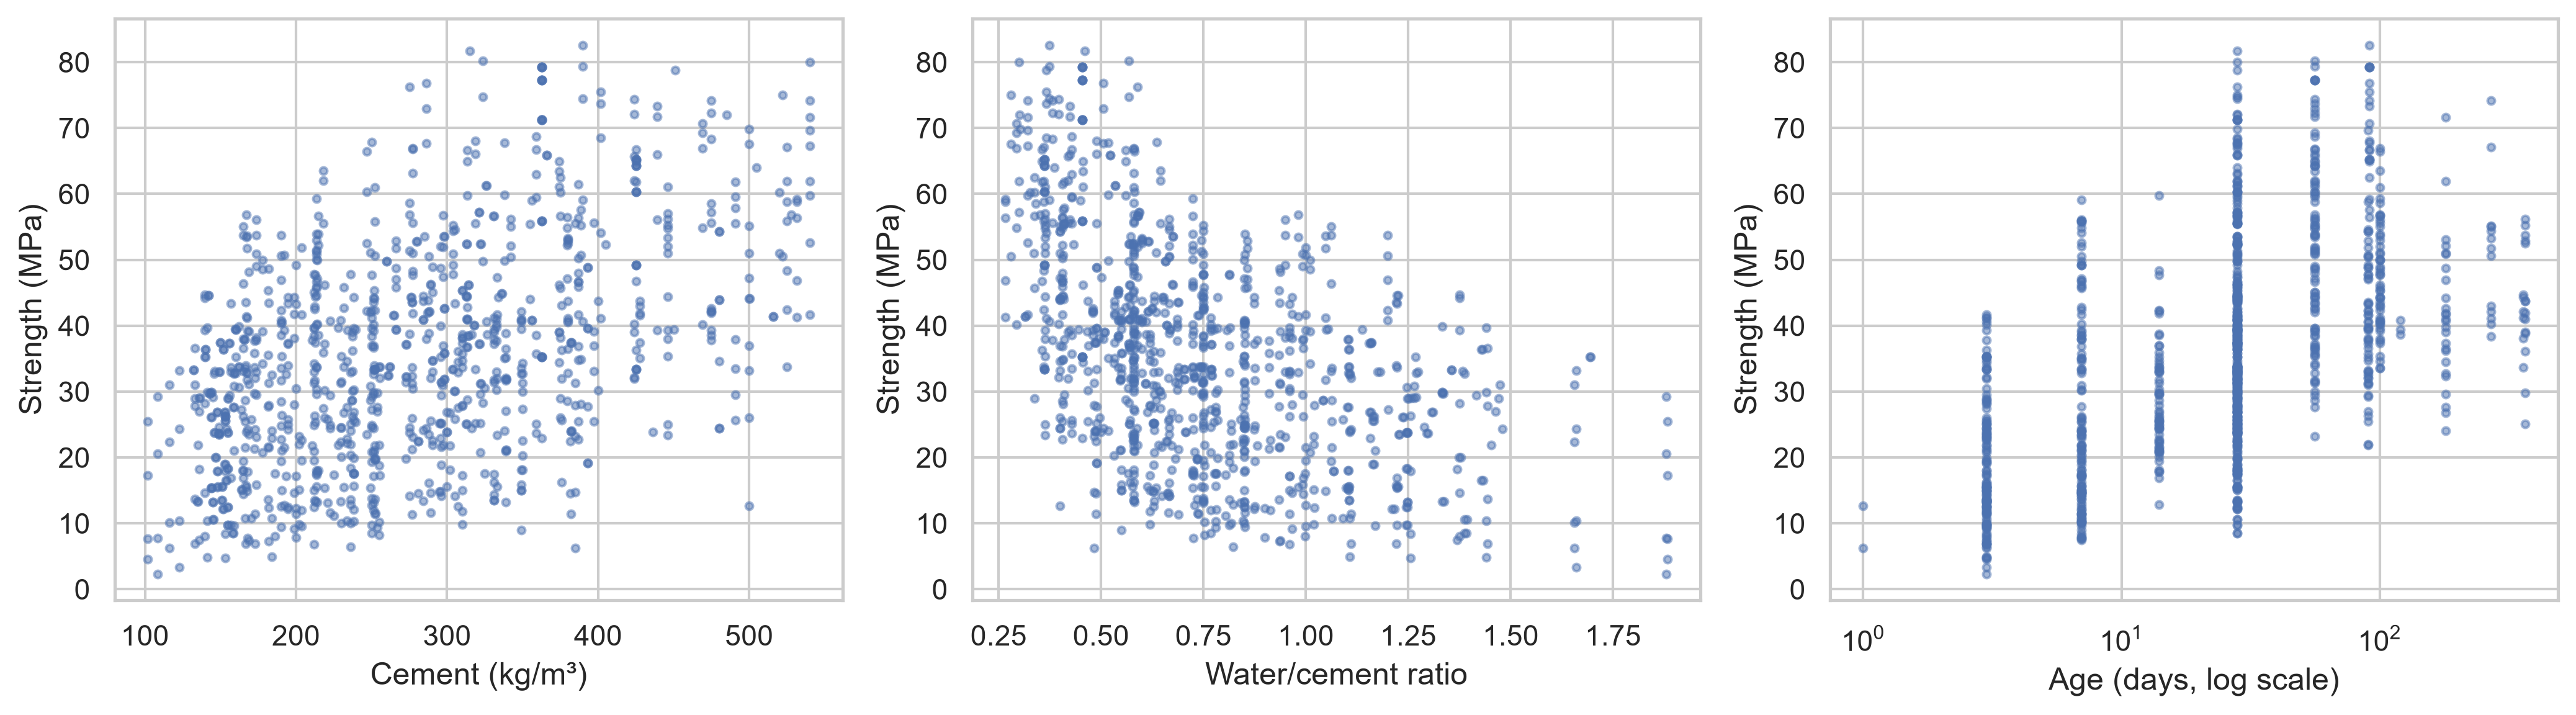
\includegraphics[keepaspectratio]{notebooks/05-regression-doe_files/figure-pdf/cell-4-output-1.png}}

Strength increases with the cement content, decreases with the
water/cement ratio (a classical rule in concrete technology, known as
Abrams' law) and grows with age -- roughly linearly in the
\emph{logarithm} of the age. We therefore enter age as
\(\ln(\text{age})\):

\begin{Shaded}
\begin{Highlighting}[]
\NormalTok{model }\OperatorTok{=}\NormalTok{ smf.ols(}\StringTok{"strength \textasciitilde{} cement + slag + fly\_ash + water + superplasticizer"}
                \StringTok{" + coarse\_agg + fine\_agg + np.log(age)"}\NormalTok{, data}\OperatorTok{=}\NormalTok{conc).fit()}
\BuiltInTok{print}\NormalTok{(model.summary())}
\end{Highlighting}
\end{Shaded}

\begin{verbatim}
                            OLS Regression Results                            
==============================================================================
Dep. Variable:               strength   R-squared:                       0.819
Model:                            OLS   Adj. R-squared:                  0.817
Method:                 Least Squares   F-statistic:                     575.6
Date:                Tue, 10 Nov 2026   Prob (F-statistic):               0.00
Time:                        14:16:35   Log-Likelihood:                -3482.4
No. Observations:                1030   AIC:                             6983.
Df Residuals:                    1021   BIC:                             7027.
Df Model:                           8                                         
Covariance Type:            nonrobust                                         
====================================================================================
                       coef    std err          t      P>|t|      [0.025      0.975]
------------------------------------------------------------------------------------
Intercept          -77.5334     18.331     -4.230      0.000    -113.504     -41.563
cement               0.1349      0.006     23.055      0.000       0.123       0.146
slag                 0.1159      0.007     16.647      0.000       0.102       0.130
fly_ash              0.0944      0.009     10.944      0.000       0.077       0.111
water               -0.1288      0.028     -4.673      0.000      -0.183      -0.075
superplasticizer     0.1188      0.064      1.846      0.065      -0.007       0.245
coarse_agg           0.0297      0.006      4.593      0.000       0.017       0.042
fine_agg             0.0360      0.007      4.886      0.000       0.022       0.050
np.log(age)          8.7466      0.192     45.610      0.000       8.370       9.123
==============================================================================
Omnibus:                       19.634   Durbin-Watson:                   1.305
Prob(Omnibus):                  0.000   Jarque-Bera (JB):               22.742
Skew:                           0.266   Prob(JB):                     1.15e-05
Kurtosis:                       3.496   Cond. No.                     1.06e+05
==============================================================================

Notes:
[1] Standard Errors assume that the covariance matrix of the errors is correctly specified.
[2] The condition number is large, 1.06e+05. This might indicate that there are
strong multicollinearity or other numerical problems.
\end{verbatim}

\textbf{Discussion.} Read the summary from top to bottom:

\begin{itemize}
\tightlist
\item
  \textbf{R² and adjusted R²} tell you how much of the variation in
  strength the model explains.
\item
  \textbf{Coefficients:} each value is the change in MPa per additional
  kg/m³ of the component (or per unit of \(\ln\) age), holding all other
  components constant. Cement, slag and fly ash act as binders and
  should have positive coefficients; water should have a negative one.
\item
  \textbf{Holding constant is tricky here:} the components add up to
  roughly the volume of one cubic metre. If we add more cement,
  something else must be reduced. This built-in dependence causes
  collinearity, which explains why some aggregate coefficients can be
  small or have surprising signs.
\item
  \textbf{Notes at the bottom:} statsmodels warns, for example, about a
  large condition number -- a hint at collinearity or very differently
  scaled inputs.
\end{itemize}

\begin{Shaded}
\begin{Highlighting}[]
\NormalTok{fig, axes }\OperatorTok{=}\NormalTok{ plt.subplots(}\DecValTok{1}\NormalTok{, }\DecValTok{3}\NormalTok{, figsize}\OperatorTok{=}\NormalTok{(}\DecValTok{14}\NormalTok{, }\DecValTok{4}\NormalTok{))}
\NormalTok{axes[}\DecValTok{0}\NormalTok{].scatter(model.fittedvalues, model.resid, s}\OperatorTok{=}\DecValTok{8}\NormalTok{, alpha}\OperatorTok{=}\FloatTok{0.5}\NormalTok{)}
\NormalTok{axes[}\DecValTok{0}\NormalTok{].axhline(}\DecValTok{0}\NormalTok{, color}\OperatorTok{=}\StringTok{"k"}\NormalTok{, lw}\OperatorTok{=}\DecValTok{1}\NormalTok{)}
\NormalTok{axes[}\DecValTok{0}\NormalTok{].}\BuiltInTok{set}\NormalTok{(xlabel}\OperatorTok{=}\StringTok{"Fitted strength (MPa)"}\NormalTok{, ylabel}\OperatorTok{=}\StringTok{"Residual (MPa)"}\NormalTok{, title}\OperatorTok{=}\StringTok{"Residuals vs fitted"}\NormalTok{)}
\NormalTok{sm.qqplot(model.resid, line}\OperatorTok{=}\StringTok{"45"}\NormalTok{, fit}\OperatorTok{=}\VariableTok{True}\NormalTok{, ax}\OperatorTok{=}\NormalTok{axes[}\DecValTok{1}\NormalTok{])}\OperatorTok{;}\NormalTok{ axes[}\DecValTok{1}\NormalTok{].set\_title(}\StringTok{"Normal QQ plot"}\NormalTok{)}
\NormalTok{axes[}\DecValTok{2}\NormalTok{].scatter(conc[}\StringTok{"age"}\NormalTok{], model.resid, s}\OperatorTok{=}\DecValTok{8}\NormalTok{, alpha}\OperatorTok{=}\FloatTok{0.5}\NormalTok{)}
\NormalTok{axes[}\DecValTok{2}\NormalTok{].}\BuiltInTok{set}\NormalTok{(xscale}\OperatorTok{=}\StringTok{"log"}\NormalTok{, xlabel}\OperatorTok{=}\StringTok{"Age (days)"}\NormalTok{, ylabel}\OperatorTok{=}\StringTok{"Residual (MPa)"}\NormalTok{, title}\OperatorTok{=}\StringTok{"Residuals vs age"}\NormalTok{)}
\NormalTok{plt.tight\_layout()}\OperatorTok{;}\NormalTok{ plt.show()}
\end{Highlighting}
\end{Shaded}

\pandocbounded{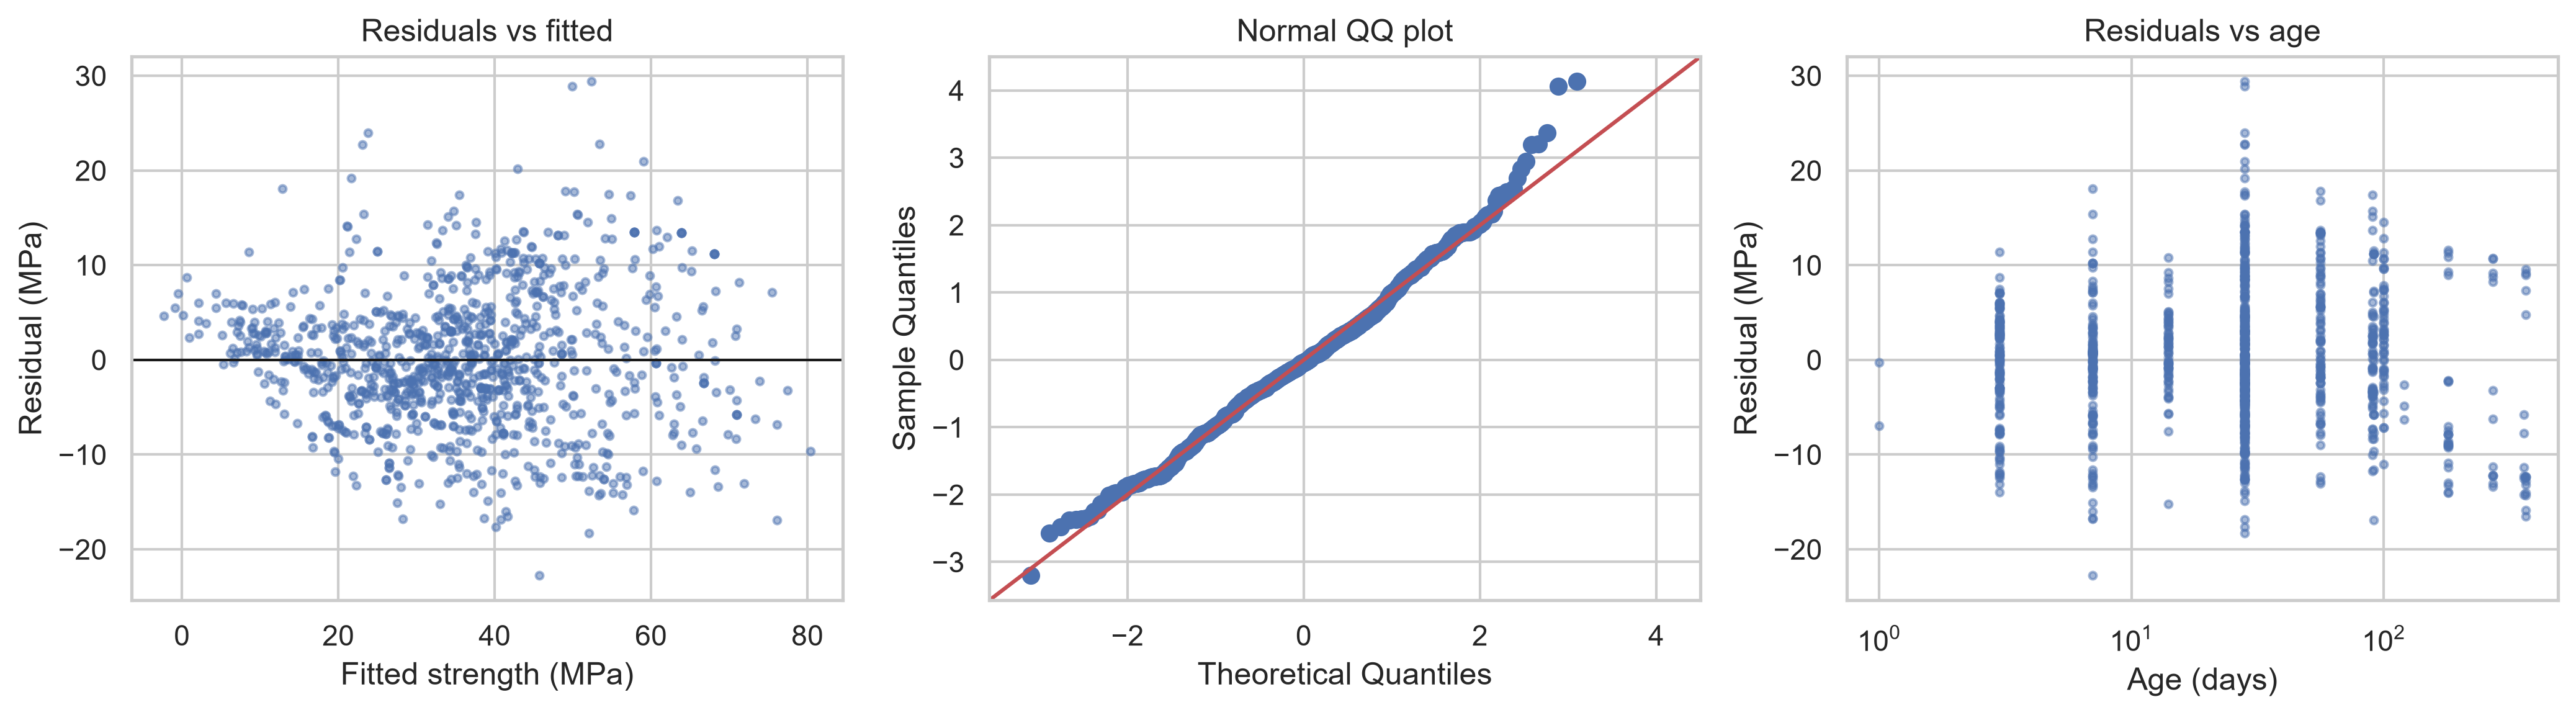
\includegraphics[keepaspectratio]{notebooks/05-regression-doe_files/figure-pdf/cell-6-output-1.png}}

\textbf{Discussion.} Look for patterns: a curved band in the residuals
vs.~fitted values indicates a missing nonlinearity; a funnel shape
indicates non-constant variance; structure in the residuals vs.~age
shows that the \(\ln\) transformation captures the age effect only
approximately. Systematic patterns tell us that the linear model is an
approximation -- which is fine for interpretation of the main effects
but limits its predictive accuracy. Flexible models in Chapters 6 and 8
will do better.

\begin{Shaded}
\begin{Highlighting}[]
\ImportTok{from}\NormalTok{ statsmodels.stats.outliers\_influence }\ImportTok{import}\NormalTok{ variance\_inflation\_factor}

\NormalTok{Xv }\OperatorTok{=}\NormalTok{ sm.add\_constant(conc[[}\StringTok{"cement"}\NormalTok{, }\StringTok{"slag"}\NormalTok{, }\StringTok{"fly\_ash"}\NormalTok{, }\StringTok{"water"}\NormalTok{, }\StringTok{"superplasticizer"}\NormalTok{,}
                          \StringTok{"coarse\_agg"}\NormalTok{, }\StringTok{"fine\_agg"}\NormalTok{]].assign(log\_age}\OperatorTok{=}\NormalTok{np.log(conc[}\StringTok{"age"}\NormalTok{])))}
\NormalTok{vif }\OperatorTok{=}\NormalTok{ pd.Series([variance\_inflation\_factor(Xv.values, i) }\ControlFlowTok{for}\NormalTok{ i }\KeywordTok{in} \BuiltInTok{range}\NormalTok{(}\DecValTok{1}\NormalTok{, Xv.shape[}\DecValTok{1}\NormalTok{])],}
\NormalTok{                index}\OperatorTok{=}\NormalTok{Xv.columns[}\DecValTok{1}\NormalTok{:], name}\OperatorTok{=}\StringTok{"VIF"}\NormalTok{)}
\NormalTok{vif.}\BuiltInTok{round}\NormalTok{(}\DecValTok{1}\NormalTok{)}
\end{Highlighting}
\end{Shaded}

\begin{verbatim}
cement              7.5
slag                7.3
fly_ash             6.1
water               7.0
superplasticizer    3.0
coarse_agg          5.1
fine_agg            7.0
log_age             1.1
Name: VIF, dtype: float64
\end{verbatim}

\subsection{Confidence vs.~prediction
intervals}\label{confidence-vs.-prediction-intervals}

A regression model gives two different kinds of intervals for a new
input \(x_0\):

\begin{tcolorbox}[enhanced jigsaw, colframe=quarto-callout-note-color-frame, toprule=.15mm, rightrule=.15mm, title=\textcolor{quarto-callout-note-color}{\faInfo}\hspace{0.5em}{Definition: Confidence interval vs.~prediction interval}, colbacktitle=quarto-callout-note-color!10!white, left=2mm, titlerule=0mm, bottomtitle=1mm, toptitle=1mm, opacityback=0, bottomrule=.15mm, breakable, arc=.35mm, opacitybacktitle=0.6, colback=white, coltitle=black, leftrule=.75mm]

\begin{itemize}
\tightlist
\item
  The \textbf{confidence interval} for the \emph{mean response}
  \(E[y \mid x_0]\) reflects only the uncertainty of the estimated
  coefficients. It shrinks towards zero as \(n\) grows.
\item
  The \textbf{prediction interval} for a \emph{single new observation}
  \(y_0\) additionally contains the scatter \(\sigma\) of individual
  observations around the mean. It never becomes narrower than about
  \(\pm 2\sigma\).
\end{itemize}

\end{tcolorbox}

\begin{figure}[H]

\centering{

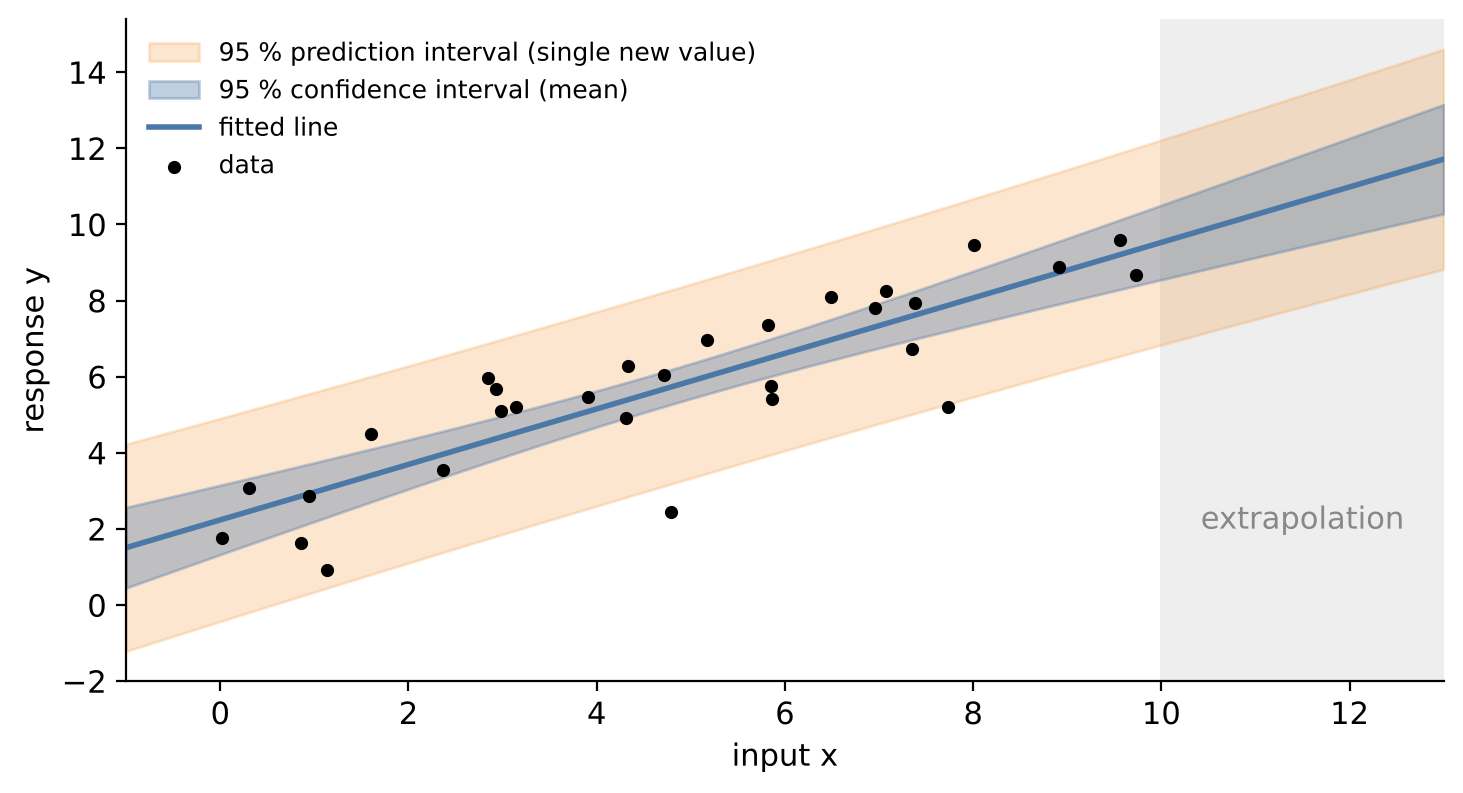
\includegraphics[width=0.85\linewidth,height=\textheight,keepaspectratio]{notebooks/images/ci-vs-pi.png}

}

\caption{\label{fig-cipi}Confidence band of the regression line (mean
response) and prediction band for single new observations. Both widen
with distance from the centre of the data -- and in the extrapolation
region, neither is supported by data.}

\end{figure}%

For an engineer who needs to know the strength of \emph{the next}
concrete batch, the prediction interval is the relevant one.

\begin{Shaded}
\begin{Highlighting}[]
\NormalTok{new\_mix }\OperatorTok{=}\NormalTok{ pd.DataFrame(\{}\StringTok{"cement"}\NormalTok{: [}\DecValTok{350}\NormalTok{], }\StringTok{"slag"}\NormalTok{: [}\DecValTok{0}\NormalTok{], }\StringTok{"fly\_ash"}\NormalTok{: [}\DecValTok{0}\NormalTok{], }\StringTok{"water"}\NormalTok{: [}\DecValTok{180}\NormalTok{],}
                        \StringTok{"superplasticizer"}\NormalTok{: [}\DecValTok{5}\NormalTok{], }\StringTok{"coarse\_agg"}\NormalTok{: [}\DecValTok{1000}\NormalTok{], }\StringTok{"fine\_agg"}\NormalTok{: [}\DecValTok{780}\NormalTok{],}
                        \StringTok{"age"}\NormalTok{: [}\DecValTok{28}\NormalTok{]\})}
\NormalTok{model.get\_prediction(new\_mix).summary\_frame(alpha}\OperatorTok{=}\FloatTok{0.05}\NormalTok{).}\BuiltInTok{round}\NormalTok{(}\DecValTok{1}\NormalTok{)}
\end{Highlighting}
\end{Shaded}

\begin{longtable}[]{@{}lllllll@{}}
\toprule\noalign{}
& mean & mean\_se & mean\_ci\_lower & mean\_ci\_upper & obs\_ci\_lower &
obs\_ci\_upper \\
\midrule\noalign{}
\endhead
\bottomrule\noalign{}
\endlastfoot
0 & 34.0 & 0.5 & 32.9 & 35.0 & 19.9 & 48.0 \\
\end{longtable}

\texttt{mean\_ci\_lower/upper} is the confidence interval of the mean
strength of such mixes at 28 days, \texttt{obs\_ci\_lower/upper} the
prediction interval for a single specimen. The difference shows how much
individual tests scatter.

\begin{tcolorbox}[enhanced jigsaw, colframe=quarto-callout-warning-color-frame, toprule=.15mm, rightrule=.15mm, title=\textcolor{quarto-callout-warning-color}{\faExclamationTriangle}\hspace{0.5em}{Pitfall: extrapolation}, colbacktitle=quarto-callout-warning-color!10!white, left=2mm, titlerule=0mm, bottomtitle=1mm, toptitle=1mm, opacityback=0, bottomrule=.15mm, breakable, arc=.35mm, opacitybacktitle=0.6, colback=white, coltitle=black, leftrule=.75mm]

Regression models are only supported by data within the range of the
inputs -- and, with correlated inputs, only within the region where
input \emph{combinations} were observed. A mix with an unusual
combination of components may lie within every single input range and
still be far from the data.

\end{tcolorbox}

\section{Nonlinear curve fitting}\label{nonlinear-curve-fitting}

Many engineering models are nonlinear in their parameters: hardening and
creep curves, exponential decay, saturation curves, characteristic
curves of components. They cannot be written as a linear model, but
their parameters can still be estimated by least squares -- numerically,
by iteration:

\[\hat\theta = \arg\min_{\theta} \sum_i \left(y_i - f(x_i; \theta)\right)^2.\]

\texttt{scipy.optimize.curve\_fit} solves this problem with the
Levenberg--Marquardt algorithm or a trust-region method.

\begin{tcolorbox}[enhanced jigsaw, colframe=quarto-callout-tip-color-frame, toprule=.15mm, rightrule=.15mm, title=\textcolor{quarto-callout-tip-color}{\faLightbulb}\hspace{0.5em}{Engineering practice: fitting physical models}, colbacktitle=quarto-callout-tip-color!10!white, left=2mm, titlerule=0mm, bottomtitle=1mm, toptitle=1mm, opacityback=0, bottomrule=.15mm, breakable, arc=.35mm, opacitybacktitle=0.6, colback=white, coltitle=black, leftrule=.75mm]

\begin{itemize}
\tightlist
\item
  \textbf{Starting values} matter: the iteration can converge to a local
  minimum or not at all. Derive them from physics or read them off a
  plot.
\item
  \textbf{Parameter uncertainty:} the covariance matrix \texttt{pcov}
  returned by \texttt{curve\_fit} gives standard errors (based on a
  linear approximation around the optimum; valid for approximately
  normal, independent errors).
\item
  \textbf{Identifiability:} if two parameters are strongly correlated,
  the data cannot separate them -- the model is too complex for the data
  or the experimental design is poor.
\item
  \textbf{Linearisation} (e.g.~fitting \(\ln y\)) is tempting but
  changes the error structure; a direct nonlinear fit is usually
  preferable.
\item
  \textbf{Physically meaningful parameters} are an advantage over a
  polynomial: they can be compared between materials and checked for
  plausibility.
\end{itemize}

\end{tcolorbox}

As an example we model the strength development of one concrete mix over
time with the hyperbolic model

\[f_c(t) = f_\infty \, \frac{t}{a + t},\]

with the final strength \(f_\infty\) (MPa) and the time \(a\) (days) at
which half of it is reached. Physically it describes a hydration process
that slows down over time.

\begin{Shaded}
\begin{Highlighting}[]
\ImportTok{from}\NormalTok{ scipy.optimize }\ImportTok{import}\NormalTok{ curve\_fit}

\NormalTok{mix\_cols }\OperatorTok{=}\NormalTok{ [}\StringTok{"cement"}\NormalTok{, }\StringTok{"slag"}\NormalTok{, }\StringTok{"fly\_ash"}\NormalTok{, }\StringTok{"water"}\NormalTok{, }\StringTok{"superplasticizer"}\NormalTok{, }\StringTok{"coarse\_agg"}\NormalTok{, }\StringTok{"fine\_agg"}\NormalTok{]}
\NormalTok{n\_ages }\OperatorTok{=}\NormalTok{ conc.groupby(mix\_cols)[}\StringTok{"age"}\NormalTok{].nunique()}
\NormalTok{best }\OperatorTok{=}\NormalTok{ n\_ages.idxmax()                                   }\CommentTok{\# the mix tested at most ages}
\NormalTok{mix }\OperatorTok{=}\NormalTok{ conc[(conc[mix\_cols] }\OperatorTok{==}\NormalTok{ pd.Series(best, index}\OperatorTok{=}\NormalTok{mix\_cols)).}\BuiltInTok{all}\NormalTok{(axis}\OperatorTok{=}\DecValTok{1}\NormalTok{)].sort\_values(}\StringTok{"age"}\NormalTok{)}
\BuiltInTok{print}\NormalTok{(}\SpecialStringTok{f"Mix tested at }\SpecialCharTok{\{}\NormalTok{n\_ages}\SpecialCharTok{.}\BuiltInTok{max}\NormalTok{()}\SpecialCharTok{\}}\SpecialStringTok{ different ages:"}\NormalTok{, }\BuiltInTok{dict}\NormalTok{(}\BuiltInTok{zip}\NormalTok{(mix\_cols, best)))}

\KeywordTok{def}\NormalTok{ strength\_model(t, f\_inf, a):}
    \ControlFlowTok{return}\NormalTok{ f\_inf }\OperatorTok{*}\NormalTok{ t }\OperatorTok{/}\NormalTok{ (a }\OperatorTok{+}\NormalTok{ t)}

\NormalTok{p0 }\OperatorTok{=}\NormalTok{ [mix[}\StringTok{"strength"}\NormalTok{].}\BuiltInTok{max}\NormalTok{(), }\DecValTok{7}\NormalTok{]                          }\CommentTok{\# starting values from the data}
\NormalTok{popt, pcov }\OperatorTok{=}\NormalTok{ curve\_fit(strength\_model, mix[}\StringTok{"age"}\NormalTok{], mix[}\StringTok{"strength"}\NormalTok{], p0}\OperatorTok{=}\NormalTok{p0)}
\NormalTok{perr }\OperatorTok{=}\NormalTok{ np.sqrt(np.diag(pcov))}
\NormalTok{corr }\OperatorTok{=}\NormalTok{ pcov[}\DecValTok{0}\NormalTok{, }\DecValTok{1}\NormalTok{] }\OperatorTok{/}\NormalTok{ (perr[}\DecValTok{0}\NormalTok{] }\OperatorTok{*}\NormalTok{ perr[}\DecValTok{1}\NormalTok{])}
\BuiltInTok{print}\NormalTok{(}\SpecialStringTok{f"f\_inf = }\SpecialCharTok{\{}\NormalTok{popt[}\DecValTok{0}\NormalTok{]}\SpecialCharTok{:.1f\}}\SpecialStringTok{ ± }\SpecialCharTok{\{}\NormalTok{perr[}\DecValTok{0}\NormalTok{]}\SpecialCharTok{:.1f\}}\SpecialStringTok{ MPa,  a = }\SpecialCharTok{\{}\NormalTok{popt[}\DecValTok{1}\NormalTok{]}\SpecialCharTok{:.1f\}}\SpecialStringTok{ ± }\SpecialCharTok{\{}\NormalTok{perr[}\DecValTok{1}\NormalTok{]}\SpecialCharTok{:.1f\}}\SpecialStringTok{ days,  "}
      \SpecialStringTok{f"correlation = }\SpecialCharTok{\{}\NormalTok{corr}\SpecialCharTok{:.2f\}}\SpecialStringTok{"}\NormalTok{)}
\end{Highlighting}
\end{Shaded}

\begin{verbatim}
Mix tested at 8 different ages: {'cement': np.float64(500.0), 'slag': np.float64(0.0), 'fly_ash': np.float64(0.0), 'water': np.float64(200.0), 'superplasticizer': np.float64(0.0), 'coarse_agg': np.float64(1125.0), 'fine_agg': np.float64(613.0)}
f_inf = 51.3 ± 1.7 MPa,  a = 3.6 ± 0.6 days,  correlation = 0.62
\end{verbatim}

\begin{Shaded}
\begin{Highlighting}[]
\CommentTok{\# 95 \% confidence band of the fitted curve (delta method)}
\NormalTok{t }\OperatorTok{=}\NormalTok{ np.linspace(}\DecValTok{1}\NormalTok{, mix[}\StringTok{"age"}\NormalTok{].}\BuiltInTok{max}\NormalTok{() }\OperatorTok{*} \FloatTok{1.1}\NormalTok{, }\DecValTok{300}\NormalTok{)}
\NormalTok{f\_inf, a }\OperatorTok{=}\NormalTok{ popt}
\NormalTok{J }\OperatorTok{=}\NormalTok{ np.column\_stack([t }\OperatorTok{/}\NormalTok{ (a }\OperatorTok{+}\NormalTok{ t), }\OperatorTok{{-}}\NormalTok{f\_inf }\OperatorTok{*}\NormalTok{ t }\OperatorTok{/}\NormalTok{ (a }\OperatorTok{+}\NormalTok{ t) }\OperatorTok{**} \DecValTok{2}\NormalTok{])   }\CommentTok{\# partial derivatives}
\NormalTok{se }\OperatorTok{=}\NormalTok{ np.sqrt(np.einsum(}\StringTok{"ij,jk,ik{-}\textgreater{}i"}\NormalTok{, J, pcov, J))}
\NormalTok{fit }\OperatorTok{=}\NormalTok{ strength\_model(t, }\OperatorTok{*}\NormalTok{popt)}

\NormalTok{plt.scatter(mix[}\StringTok{"age"}\NormalTok{], mix[}\StringTok{"strength"}\NormalTok{], label}\OperatorTok{=}\StringTok{"measurements"}\NormalTok{, zorder}\OperatorTok{=}\DecValTok{3}\NormalTok{)}
\NormalTok{plt.plot(t, fit, label}\OperatorTok{=}\StringTok{"nonlinear fit"}\NormalTok{)}
\NormalTok{plt.fill\_between(t, fit }\OperatorTok{{-}} \FloatTok{1.96} \OperatorTok{*}\NormalTok{ se, fit }\OperatorTok{+} \FloatTok{1.96} \OperatorTok{*}\NormalTok{ se, alpha}\OperatorTok{=}\FloatTok{0.25}\NormalTok{, label}\OperatorTok{=}\StringTok{"95 }\SpecialCharTok{\% c}\StringTok{onfidence band"}\NormalTok{)}
\NormalTok{plt.axhline(f\_inf, ls}\OperatorTok{=}\StringTok{":"}\NormalTok{, c}\OperatorTok{=}\StringTok{"k"}\NormalTok{, lw}\OperatorTok{=}\DecValTok{1}\NormalTok{)}
\NormalTok{plt.xlabel(}\StringTok{"Age (days)"}\NormalTok{)}\OperatorTok{;}\NormalTok{ plt.ylabel(}\StringTok{"Compressive strength (MPa)"}\NormalTok{)}\OperatorTok{;}\NormalTok{ plt.legend()}
\NormalTok{plt.show()}
\end{Highlighting}
\end{Shaded}

\pandocbounded{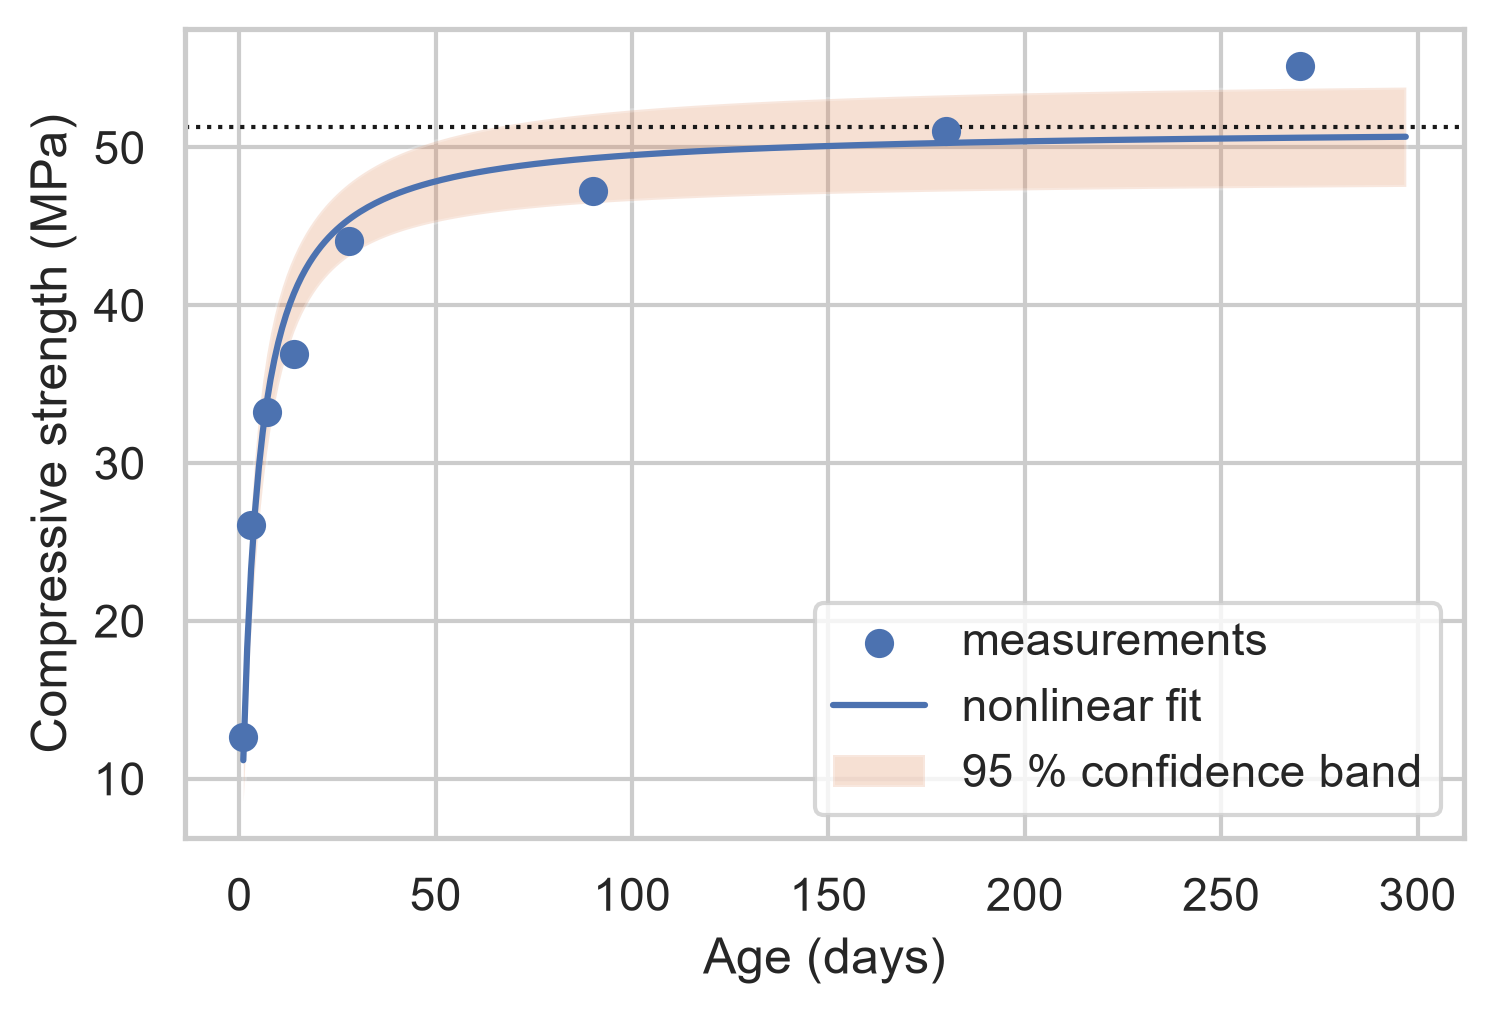
\includegraphics[keepaspectratio]{notebooks/05-regression-doe_files/figure-pdf/cell-10-output-1.png}}

\textbf{Discussion.} The two parameters have a direct engineering
meaning and can be compared between mixes. The confidence band is
computed with the \textbf{delta method}: the variance of the fitted
curve is approximated by \(J\,\text{Cov}(\hat\theta)\,J^\top\), where
\(J\) contains the partial derivatives of the model with respect to the
parameters. The band is narrow where many measurements exist and widens
towards long ages. A strong correlation between \(\hat f_\infty\) and
\(\hat a\) is typical for saturation models: if the data do not reach
the plateau, a higher final strength reached later explains them almost
equally well.

\section{Back to the decision}\label{back-to-the-decision-4}

A strength promise concerns \emph{individual} elements, not the average
of many -- so the relevant interval is the \textbf{prediction interval}.
To be on the safe side, we require that the lower end of the 95 \%
prediction interval reaches 35 MPa. We check 28 days and, if necessary,
search for the earliest age at which the requirement is met.

\begin{Shaded}
\begin{Highlighting}[]
\NormalTok{required }\OperatorTok{=} \FloatTok{35.0}
\NormalTok{ages }\OperatorTok{=}\NormalTok{ np.arange(}\DecValTok{1}\NormalTok{, }\DecValTok{366}\NormalTok{)}
\NormalTok{candidates }\OperatorTok{=}\NormalTok{ pd.concat([new\_mix.drop(columns}\OperatorTok{=}\StringTok{"age"}\NormalTok{)] }\OperatorTok{*} \BuiltInTok{len}\NormalTok{(ages), ignore\_index}\OperatorTok{=}\VariableTok{True}\NormalTok{).assign(age}\OperatorTok{=}\NormalTok{ages)}
\NormalTok{pi\_low }\OperatorTok{=}\NormalTok{ model.get\_prediction(candidates).summary\_frame(alpha}\OperatorTok{=}\FloatTok{0.05}\NormalTok{)[}\StringTok{"obs\_ci\_lower"}\NormalTok{].values}
\NormalTok{low\_28 }\OperatorTok{=}\NormalTok{ pi\_low[ages }\OperatorTok{==} \DecValTok{28}\NormalTok{][}\DecValTok{0}\NormalTok{]}
\BuiltInTok{print}\NormalTok{(}\SpecialStringTok{f"Lower 95 \% prediction bound at 28 days: }\SpecialCharTok{\{}\NormalTok{low\_28}\SpecialCharTok{:.1f\}}\SpecialStringTok{ MPa"}\NormalTok{)}
\ControlFlowTok{if}\NormalTok{ low\_28 }\OperatorTok{\textgreater{}=}\NormalTok{ required:}
    \BuiltInTok{print}\NormalTok{(}\StringTok{"Decision: approve the mix for the 28{-}day promise."}\NormalTok{)}
\ControlFlowTok{elif}\NormalTok{ (pi\_low }\OperatorTok{\textgreater{}=}\NormalTok{ required).}\BuiltInTok{any}\NormalTok{():}
    \BuiltInTok{print}\NormalTok{(}\SpecialStringTok{f"Decision: not at 28 days – promise }\SpecialCharTok{\{}\NormalTok{ages[np.argmax(pi\_low }\OperatorTok{\textgreater{}=}\NormalTok{ required)]}\SpecialCharTok{\}}\SpecialStringTok{ days, or confirm with test specimens."}\NormalTok{)}
\ControlFlowTok{else}\NormalTok{:}
    \BuiltInTok{print}\NormalTok{(}\StringTok{"Decision: the model cannot guarantee 35 MPa within a year – adjust the mix (e.g. lower w/c ratio)."}\NormalTok{)}
\end{Highlighting}
\end{Shaded}

\begin{verbatim}
Lower 95 % prediction bound at 28 days: 19.9 MPa
Decision: not at 28 days – promise 158 days, or confirm with test specimens.
\end{verbatim}

The recommendation should also state the limits of the model: it is a
linear approximation fitted to laboratory specimens from one study, and
the residual analysis showed systematic deviations. In practice, no
plant would release a new mix on the basis of a regression model alone
-- but the model tells us whether the trial batches are worth casting
and which test age to plan.

\section{Extension: design of experiments -- a 2³ full factorial
design}\label{extension-design-of-experiments-a-2uxb3-full-factorial-design}

\emph{Extension -- optional material, not required for the exam.}

The concrete data are \emph{observational}: the mixes were not chosen to
estimate effects efficiently, and the inputs are correlated. In a
\textbf{designed experiment} we choose the factor settings ourselves, so
that the effects can be separated cleanly with as few runs as possible.

\begin{tcolorbox}[enhanced jigsaw, colframe=quarto-callout-note-color-frame, toprule=.15mm, rightrule=.15mm, title=\textcolor{quarto-callout-note-color}{\faInfo}\hspace{0.5em}{Definition: Full factorial design}, colbacktitle=quarto-callout-note-color!10!white, left=2mm, titlerule=0mm, bottomtitle=1mm, toptitle=1mm, opacityback=0, bottomrule=.15mm, breakable, arc=.35mm, opacitybacktitle=0.6, colback=white, coltitle=black, leftrule=.75mm]

In a \(2^k\) full factorial design, each of \(k\) factors is set to a
low (−1) and a high (+1) level, and all \(2^k\) combinations are run.
The columns of the coded design matrix are \textbf{orthogonal}, so all
main effects and interactions are estimated independently of each other
and with the smallest possible variance.

\end{tcolorbox}

With three factors, 8 runs estimate 3 main effects, 3 two-factor
interactions and 1 three-factor interaction. \textbf{Replicates}
(repeating all runs) provide an estimate of the experimental error.
\textbf{Randomising} the run order protects against drifts in the test
setup.

The example simulates such an experiment with a known ``true'' model, so
we can check whether the analysis recovers it.

\begin{Shaded}
\begin{Highlighting}[]
\ImportTok{import}\NormalTok{ itertools}

\NormalTok{design }\OperatorTok{=}\NormalTok{ pd.DataFrame(}\BuiltInTok{list}\NormalTok{(itertools.product([}\OperatorTok{{-}}\DecValTok{1}\NormalTok{, }\DecValTok{1}\NormalTok{], repeat}\OperatorTok{=}\DecValTok{3}\NormalTok{)),}
\NormalTok{                      columns}\OperatorTok{=}\NormalTok{[}\StringTok{"cement"}\NormalTok{, }\StringTok{"water"}\NormalTok{, }\StringTok{"age"}\NormalTok{])}
\NormalTok{rng }\OperatorTok{=}\NormalTok{ np.random.default\_rng(}\DecValTok{42}\NormalTok{)}
\NormalTok{design }\OperatorTok{=}\NormalTok{ pd.concat([design, design], ignore\_index}\OperatorTok{=}\VariableTok{True}\NormalTok{)        }\CommentTok{\# 2 replicates}
\NormalTok{design[}\StringTok{"strength"}\NormalTok{] }\OperatorTok{=}\NormalTok{ (}\DecValTok{40} \OperatorTok{+} \DecValTok{8} \OperatorTok{*}\NormalTok{ design.cement }\OperatorTok{{-}} \DecValTok{6} \OperatorTok{*}\NormalTok{ design.water }\OperatorTok{+} \DecValTok{5} \OperatorTok{*}\NormalTok{ design.age}
                      \OperatorTok{+} \DecValTok{2} \OperatorTok{*}\NormalTok{ design.cement }\OperatorTok{*}\NormalTok{ design.age }\OperatorTok{+}\NormalTok{ rng.normal(}\DecValTok{0}\NormalTok{, }\FloatTok{1.5}\NormalTok{, }\BuiltInTok{len}\NormalTok{(design)))}

\NormalTok{doe }\OperatorTok{=}\NormalTok{ smf.ols(}\StringTok{"strength \textasciitilde{} cement * water * age"}\NormalTok{, data}\OperatorTok{=}\NormalTok{design).fit()}
\BuiltInTok{print}\NormalTok{(doe.params.}\BuiltInTok{round}\NormalTok{(}\DecValTok{2}\NormalTok{))}
\BuiltInTok{print}\NormalTok{(}\StringTok{"Correlation between design columns:}\CharTok{\textbackslash{}n}\StringTok{"}\NormalTok{,}
\NormalTok{      np.}\BuiltInTok{round}\NormalTok{(np.corrcoef(design[[}\StringTok{"cement"}\NormalTok{, }\StringTok{"water"}\NormalTok{, }\StringTok{"age"}\NormalTok{]].T.values), }\DecValTok{2}\NormalTok{))}
\end{Highlighting}
\end{Shaded}

\begin{verbatim}
Intercept           39.92
cement               7.59
water               -5.40
cement:water        -0.33
age                  4.80
cement:age           2.19
water:age           -0.11
cement:water:age    -0.54
dtype: float64
Correlation between design columns:
 [[1. 0. 0.]
 [0. 1. 0.]
 [0. 0. 1.]]
\end{verbatim}

The estimated coefficients reproduce the true values (8, −6, 5 and 2 for
the cement × age interaction) up to the noise, and the non-existing
interactions are estimated near zero. With coded factors, a coefficient
is half the \textbf{effect} (change of the response from the low to the
high level). The design columns are uncorrelated -- the exact opposite
of the observational concrete data.

\begin{tcolorbox}[enhanced jigsaw, colframe=quarto-callout-important-color-frame, toprule=.15mm, rightrule=.15mm, title=\textcolor{quarto-callout-important-color}{\faExclamation}\hspace{0.5em}{Key takeaways}, colbacktitle=quarto-callout-important-color!10!white, left=2mm, titlerule=0mm, bottomtitle=1mm, toptitle=1mm, opacityback=0, bottomrule=.15mm, breakable, arc=.35mm, opacitybacktitle=0.6, colback=white, coltitle=black, leftrule=.75mm]

\begin{itemize}
\tightlist
\item
  Linear regression is linear in the parameters; transformations and
  interactions make it flexible.
\item
  Coefficients mean ``change per unit, all else constant'' --
  collinearity makes this hard to interpret.
\item
  Check residuals for patterns; R² alone does not validate a model.
\item
  Use prediction intervals for single new observations; beware of
  extrapolation.
\item
  Nonlinear models with physically meaningful parameters are fitted with
  \texttt{curve\_fit}; good starting values and parameter correlations
  deserve attention.
\end{itemize}

\end{tcolorbox}

\section{Exercises}\label{exercises-4}

\begin{enumerate}
\def\labelenumi{\arabic{enumi}.}
\tightlist
\item
  Replace \texttt{np.log(age)} by \texttt{age} in the linear model. How
  do R² and the residual plot change? Explain physically why the log
  transform helps.
\item
  Compute the water/cement ratio and use it as an input instead of
  \texttt{water} and \texttt{cement}. Compare R² and interpretability
  with the original model.
\item
  Which coefficients of the concrete model are statistically
  significant? Are the signs plausible from a materials point of view?
  Relate your answer to the VIF values.
\item
  Fit the strength model \(f_\infty\,t/(a+t)\) to all mixes with at
  least four test ages. How does the final strength \(f_\infty\) depend
  on the water/cement ratio?
\item
  Compare the hyperbolic model with a logarithmic model
  \(f(t) = c_0 + c_1 \ln t\) for the selected mix. Which one
  extrapolates more plausibly to 1000 days, and why is extrapolation
  risky anyway?
\item
  (Extension) Extend the DoE example to a \(2^4\) design with a fourth
  factor. How many runs are needed? What is a fractional factorial
  design, and what is its price?
\end{enumerate}

\subsection{Solutions}\label{solutions-4}

\begin{tcolorbox}[enhanced jigsaw, colframe=quarto-callout-caution-color-frame, toprule=.15mm, rightrule=.15mm, title=\textcolor{quarto-callout-caution-color}{\faFire}\hspace{0.5em}{Solution to Exercise 1}, colbacktitle=quarto-callout-caution-color!10!white, left=2mm, titlerule=0mm, bottomtitle=1mm, toptitle=1mm, opacityback=0, bottomrule=.15mm, breakable, arc=.35mm, opacitybacktitle=0.6, colback=white, coltitle=black, leftrule=.75mm]

\begin{Shaded}
\begin{Highlighting}[]
\NormalTok{model\_lin\_age }\OperatorTok{=}\NormalTok{ smf.ols(}\StringTok{"strength \textasciitilde{} cement + slag + fly\_ash + water + superplasticizer"}
                        \StringTok{" + coarse\_agg + fine\_agg + age"}\NormalTok{, data}\OperatorTok{=}\NormalTok{conc).fit()}
\BuiltInTok{print}\NormalTok{(}\SpecialStringTok{f"R² with log(age): }\SpecialCharTok{\{}\NormalTok{model}\SpecialCharTok{.}\NormalTok{rsquared}\SpecialCharTok{:.3f\}}\SpecialStringTok{,  with age: }\SpecialCharTok{\{}\NormalTok{model\_lin\_age}\SpecialCharTok{.}\NormalTok{rsquared}\SpecialCharTok{:.3f\}}\SpecialStringTok{"}\NormalTok{)}
\NormalTok{plt.scatter(conc[}\StringTok{"age"}\NormalTok{], model\_lin\_age.resid, s}\OperatorTok{=}\DecValTok{8}\NormalTok{, alpha}\OperatorTok{=}\FloatTok{0.5}\NormalTok{)}
\NormalTok{plt.axhline(}\DecValTok{0}\NormalTok{, c}\OperatorTok{=}\StringTok{"k"}\NormalTok{)}\OperatorTok{;}\NormalTok{ plt.xscale(}\StringTok{"log"}\NormalTok{)}\OperatorTok{;}\NormalTok{ plt.xlabel(}\StringTok{"Age (days)"}\NormalTok{)}\OperatorTok{;}\NormalTok{ plt.ylabel(}\StringTok{"Residual (MPa)"}\NormalTok{)}
\NormalTok{plt.show()}
\end{Highlighting}
\end{Shaded}

\begin{verbatim}
R² with log(age): 0.819,  with age: 0.616
\end{verbatim}

\pandocbounded{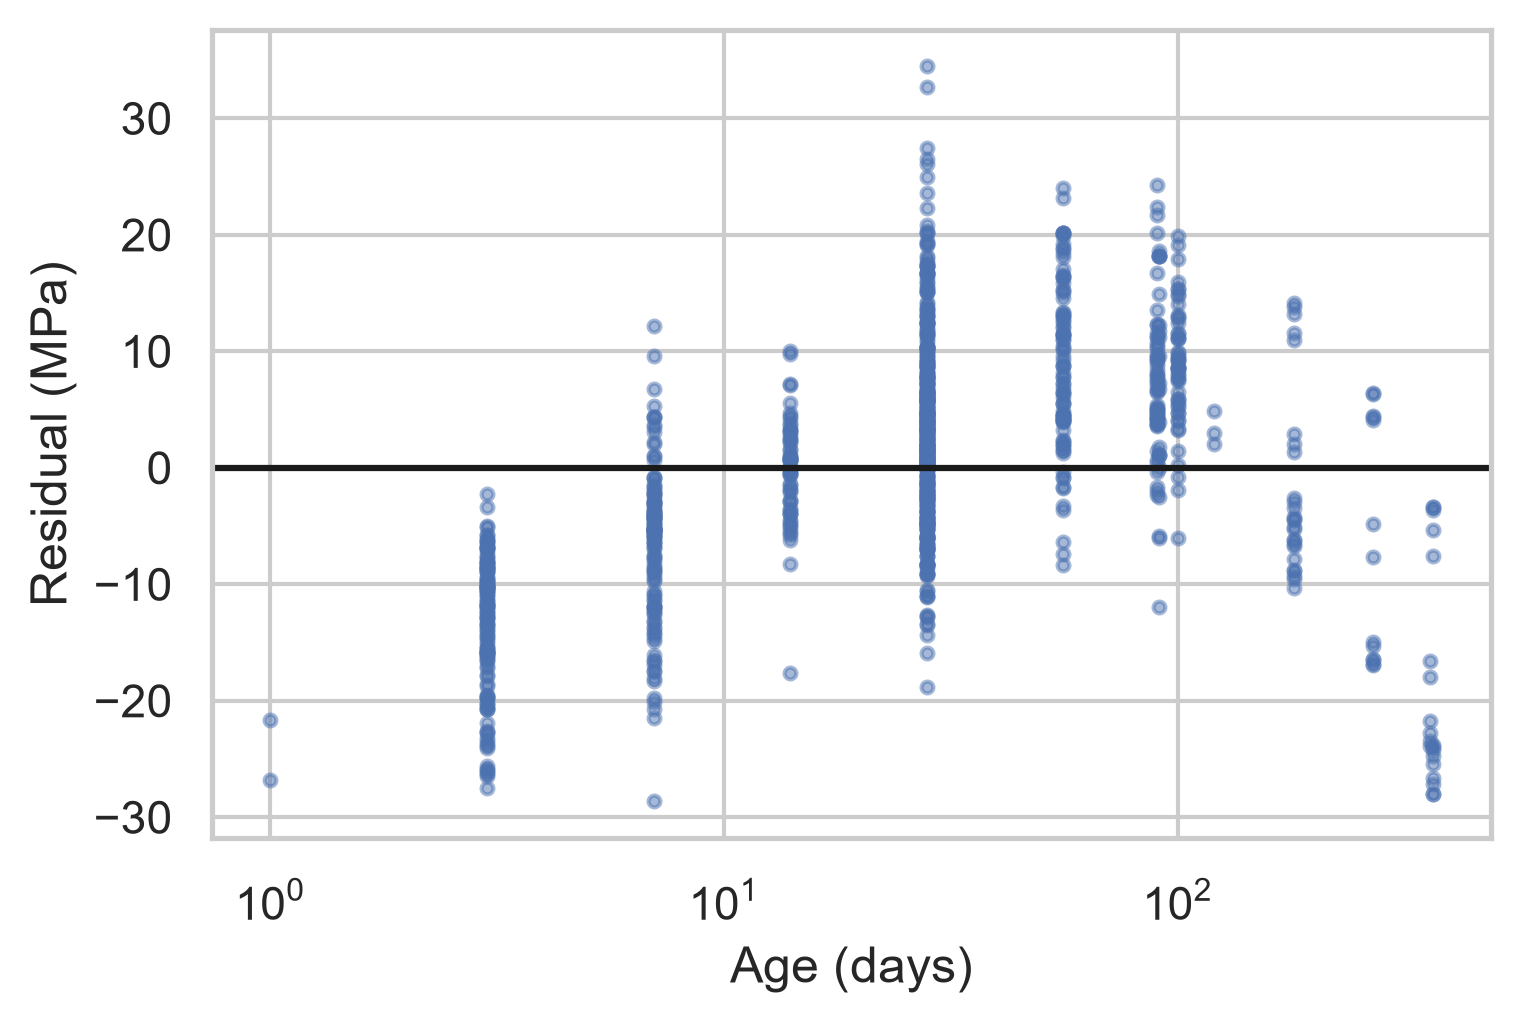
\includegraphics[keepaspectratio]{notebooks/05-regression-doe_files/figure-pdf/cell-13-output-2.png}}

With a linear age term, R² drops noticeably and the residuals show a
clear curved pattern over age: the model overestimates young and very
old specimens and underestimates intermediate ages. Physically,
hydration of cement is fast in the first days and slows down later --
the strength gain per day decreases with age. \(\ln(\text{age})\)
captures this diminishing return.

\end{tcolorbox}

\begin{tcolorbox}[enhanced jigsaw, colframe=quarto-callout-caution-color-frame, toprule=.15mm, rightrule=.15mm, title=\textcolor{quarto-callout-caution-color}{\faFire}\hspace{0.5em}{Solution to Exercise 2}, colbacktitle=quarto-callout-caution-color!10!white, left=2mm, titlerule=0mm, bottomtitle=1mm, toptitle=1mm, opacityback=0, bottomrule=.15mm, breakable, arc=.35mm, opacitybacktitle=0.6, colback=white, coltitle=black, leftrule=.75mm]

\begin{Shaded}
\begin{Highlighting}[]
\NormalTok{conc[}\StringTok{"wc"}\NormalTok{] }\OperatorTok{=}\NormalTok{ conc[}\StringTok{"water"}\NormalTok{] }\OperatorTok{/}\NormalTok{ conc[}\StringTok{"cement"}\NormalTok{]}
\NormalTok{model\_wc }\OperatorTok{=}\NormalTok{ smf.ols(}\StringTok{"strength \textasciitilde{} wc + slag + fly\_ash + superplasticizer"}
                   \StringTok{" + coarse\_agg + fine\_agg + np.log(age)"}\NormalTok{, data}\OperatorTok{=}\NormalTok{conc).fit()}
\BuiltInTok{print}\NormalTok{(}\SpecialStringTok{f"R²: original }\SpecialCharTok{\{}\NormalTok{model}\SpecialCharTok{.}\NormalTok{rsquared}\SpecialCharTok{:.3f\}}\SpecialStringTok{, with w/c ratio }\SpecialCharTok{\{}\NormalTok{model\_wc}\SpecialCharTok{.}\NormalTok{rsquared}\SpecialCharTok{:.3f\}}\SpecialStringTok{"}\NormalTok{)}
\NormalTok{model\_wc.params.}\BuiltInTok{round}\NormalTok{(}\DecValTok{3}\NormalTok{)}
\end{Highlighting}
\end{Shaded}

\begin{verbatim}
R²: original 0.819, with w/c ratio 0.759
\end{verbatim}

\begin{verbatim}
Intercept           21.087
wc                 -35.379
slag                 0.083
fly_ash              0.036
superplasticizer     0.475
coarse_agg           0.001
fine_agg             0.003
np.log(age)          8.240
dtype: float64
\end{verbatim}

The fit is of similar quality -- the w/c ratio carries most of the
information of water and cement together. The advantage is
interpretability: the coefficient of \texttt{wc} directly expresses the
well-known strength loss with increasing water/cement ratio, a quantity
concrete engineers think in. Strictly, Abrams' law is nonlinear
(strength ∝ \(B^{-w/c}\) with a material constant \(B\)), so
\(\ln(\text{strength})\) vs.~\texttt{wc} might fit even better.

\end{tcolorbox}

\begin{tcolorbox}[enhanced jigsaw, colframe=quarto-callout-caution-color-frame, toprule=.15mm, rightrule=.15mm, title=\textcolor{quarto-callout-caution-color}{\faFire}\hspace{0.5em}{Solution to Exercise 3}, colbacktitle=quarto-callout-caution-color!10!white, left=2mm, titlerule=0mm, bottomtitle=1mm, toptitle=1mm, opacityback=0, bottomrule=.15mm, breakable, arc=.35mm, opacitybacktitle=0.6, colback=white, coltitle=black, leftrule=.75mm]

\begin{Shaded}
\begin{Highlighting}[]
\NormalTok{pd.DataFrame(\{}\StringTok{"coef"}\NormalTok{: model.params, }\StringTok{"p"}\NormalTok{: model.pvalues, }\StringTok{"VIF"}\NormalTok{: vif\}).}\BuiltInTok{round}\NormalTok{(}\DecValTok{4}\NormalTok{)}
\end{Highlighting}
\end{Shaded}

\begin{longtable}[]{@{}llll@{}}
\toprule\noalign{}
& coef & p & VIF \\
\midrule\noalign{}
\endhead
\bottomrule\noalign{}
\endlastfoot
Intercept & -77.5334 & 0.0000 & NaN \\
cement & 0.1349 & 0.0000 & 7.5324 \\
coarse\_agg & 0.0297 & 0.0000 & 5.0890 \\
fine\_agg & 0.0360 & 0.0000 & 7.0304 \\
fly\_ash & 0.0944 & 0.0000 & 6.1411 \\
log\_age & NaN & NaN & 1.0523 \\
np.log(age) & 8.7466 & 0.0000 & NaN \\
slag & 0.1159 & 0.0000 & 7.2792 \\
superplasticizer & 0.1188 & 0.0652 & 2.9803 \\
water & -0.1288 & 0.0000 & 6.9839 \\
\end{longtable}

Expected signs: cement, slag and fly ash (binders) and superplasticizer
positive; water negative; age positive. Coefficients that are not
significant or have counterintuitive signs typically belong to inputs
with high VIF -- the aggregates, which are strongly linked to the other
components through the fixed total volume. Their individual coefficients
cannot be interpreted reliably, even though the model as a whole
predicts reasonably.

\end{tcolorbox}

\begin{tcolorbox}[enhanced jigsaw, colframe=quarto-callout-caution-color-frame, toprule=.15mm, rightrule=.15mm, title=\textcolor{quarto-callout-caution-color}{\faFire}\hspace{0.5em}{Solution to Exercise 4}, colbacktitle=quarto-callout-caution-color!10!white, left=2mm, titlerule=0mm, bottomtitle=1mm, toptitle=1mm, opacityback=0, bottomrule=.15mm, breakable, arc=.35mm, opacitybacktitle=0.6, colback=white, coltitle=black, leftrule=.75mm]

\begin{Shaded}
\begin{Highlighting}[]
\NormalTok{rows }\OperatorTok{=}\NormalTok{ []}
\ControlFlowTok{for}\NormalTok{ key, g }\KeywordTok{in}\NormalTok{ conc.groupby(mix\_cols):}
    \ControlFlowTok{if}\NormalTok{ g[}\StringTok{"age"}\NormalTok{].nunique() }\OperatorTok{\textless{}} \DecValTok{4}\NormalTok{:}
        \ControlFlowTok{continue}
    \ControlFlowTok{try}\NormalTok{:}
\NormalTok{        p, \_ }\OperatorTok{=}\NormalTok{ curve\_fit(strength\_model, g[}\StringTok{"age"}\NormalTok{], g[}\StringTok{"strength"}\NormalTok{],}
\NormalTok{                         p0}\OperatorTok{=}\NormalTok{[g[}\StringTok{"strength"}\NormalTok{].}\BuiltInTok{max}\NormalTok{(), }\DecValTok{7}\NormalTok{], maxfev}\OperatorTok{=}\DecValTok{5000}\NormalTok{)}
    \ControlFlowTok{except} \PreprocessorTok{RuntimeError}\NormalTok{:}
        \ControlFlowTok{continue}                                          \CommentTok{\# fit did not converge}
\NormalTok{    rows.append(\{}\StringTok{"wc"}\NormalTok{: g[}\StringTok{"water"}\NormalTok{].iloc[}\DecValTok{0}\NormalTok{] }\OperatorTok{/}\NormalTok{ g[}\StringTok{"cement"}\NormalTok{].iloc[}\DecValTok{0}\NormalTok{], }\StringTok{"f\_inf"}\NormalTok{: p[}\DecValTok{0}\NormalTok{], }\StringTok{"a"}\NormalTok{: p[}\DecValTok{1}\NormalTok{]\})}
\NormalTok{fits }\OperatorTok{=}\NormalTok{ pd.DataFrame(rows)}
\NormalTok{fits }\OperatorTok{=}\NormalTok{ fits[(fits[}\StringTok{"a"}\NormalTok{] }\OperatorTok{\textgreater{}} \DecValTok{0}\NormalTok{) }\OperatorTok{\&}\NormalTok{ (fits[}\StringTok{"f\_inf"}\NormalTok{] }\OperatorTok{\textless{}} \DecValTok{200}\NormalTok{)]        }\CommentTok{\# drop physically meaningless fits}
\NormalTok{plt.scatter(fits[}\StringTok{"wc"}\NormalTok{], fits[}\StringTok{"f\_inf"}\NormalTok{])}
\NormalTok{plt.xlabel(}\StringTok{"Water/cement ratio"}\NormalTok{)}\OperatorTok{;}\NormalTok{ plt.ylabel(}\StringTok{"Fitted final strength f\_inf (MPa)"}\NormalTok{)}
\NormalTok{plt.show()}
\BuiltInTok{print}\NormalTok{(}\SpecialStringTok{f"}\SpecialCharTok{\{}\BuiltInTok{len}\NormalTok{(fits)}\SpecialCharTok{\}}\SpecialStringTok{ mixes fitted"}\NormalTok{)}
\end{Highlighting}
\end{Shaded}

\pandocbounded{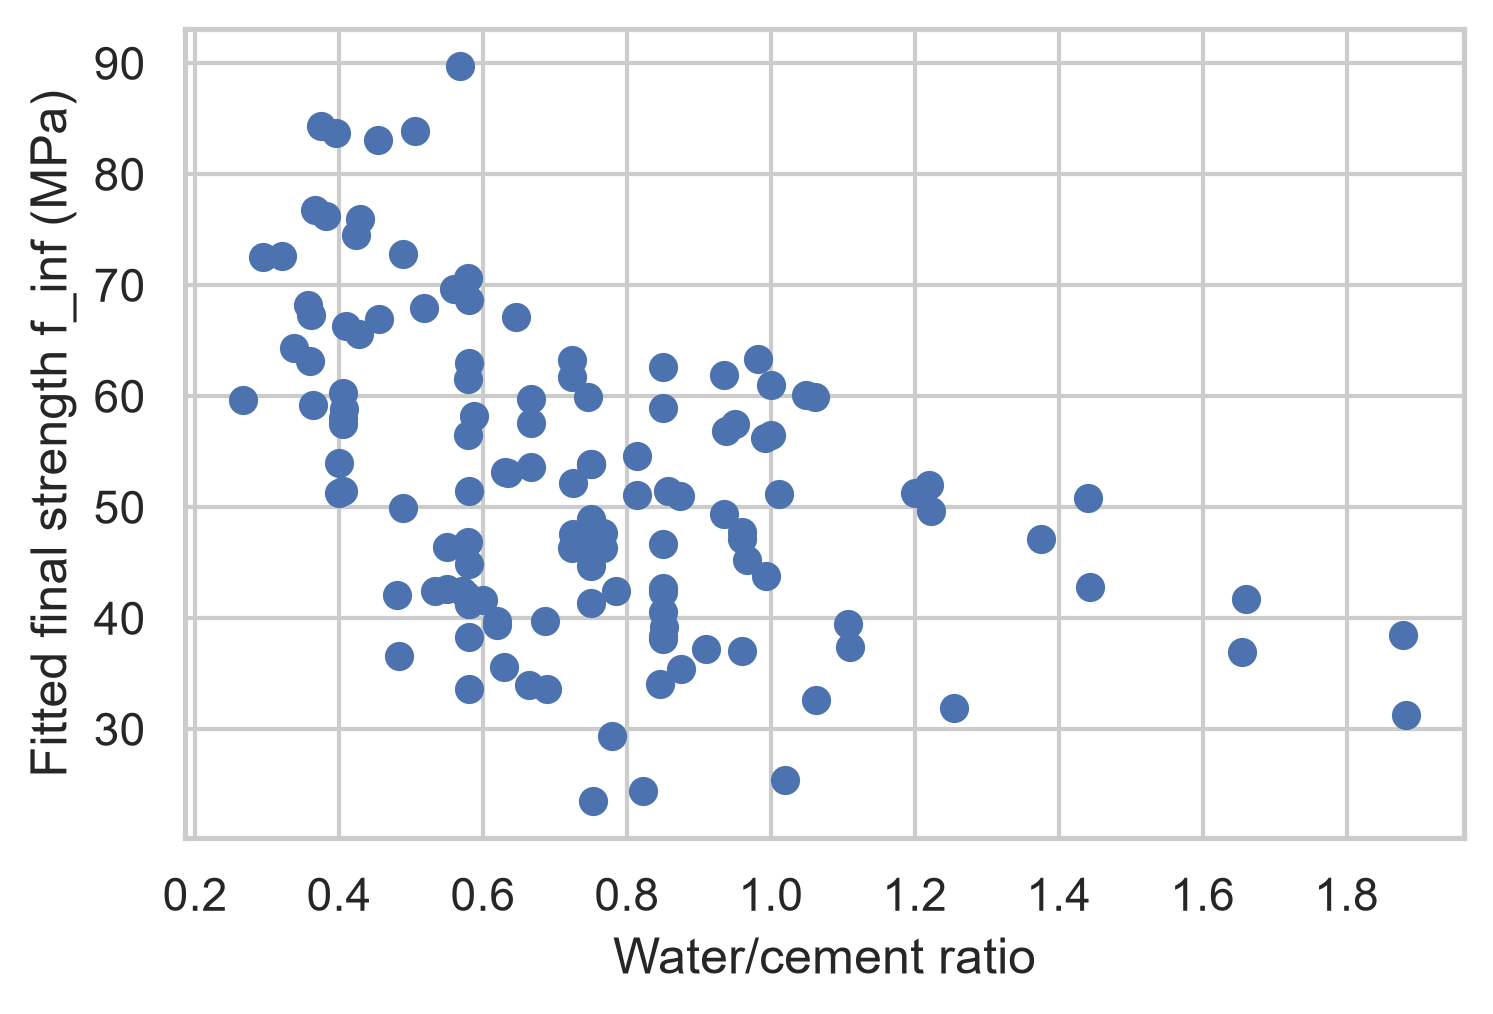
\includegraphics[keepaspectratio]{notebooks/05-regression-doe_files/figure-pdf/cell-16-output-1.png}}

\begin{verbatim}
131 mixes fitted
\end{verbatim}

The final strength decreases clearly with increasing water/cement ratio
-- the same relationship as in the linear model, but now expressed
through a physically meaningful parameter. Some fits must be discarded
because the mix was tested at too few or too early ages to determine the
plateau (the parameters are then not identifiable). Checking
plausibility of fitted parameters is an essential step when fitting many
curves automatically.

\end{tcolorbox}

\begin{tcolorbox}[enhanced jigsaw, colframe=quarto-callout-caution-color-frame, toprule=.15mm, rightrule=.15mm, title=\textcolor{quarto-callout-caution-color}{\faFire}\hspace{0.5em}{Solution to Exercise 5}, colbacktitle=quarto-callout-caution-color!10!white, left=2mm, titlerule=0mm, bottomtitle=1mm, toptitle=1mm, opacityback=0, bottomrule=.15mm, breakable, arc=.35mm, opacitybacktitle=0.6, colback=white, coltitle=black, leftrule=.75mm]

\begin{Shaded}
\begin{Highlighting}[]
\NormalTok{c1, c0 }\OperatorTok{=}\NormalTok{ np.polyfit(np.log(mix[}\StringTok{"age"}\NormalTok{]), mix[}\StringTok{"strength"}\NormalTok{], deg}\OperatorTok{=}\DecValTok{1}\NormalTok{)}
\NormalTok{t\_long }\OperatorTok{=}\NormalTok{ np.linspace(}\DecValTok{1}\NormalTok{, }\DecValTok{1000}\NormalTok{, }\DecValTok{400}\NormalTok{)}
\NormalTok{plt.scatter(mix[}\StringTok{"age"}\NormalTok{], mix[}\StringTok{"strength"}\NormalTok{], zorder}\OperatorTok{=}\DecValTok{3}\NormalTok{, label}\OperatorTok{=}\StringTok{"measurements"}\NormalTok{)}
\NormalTok{plt.plot(t\_long, strength\_model(t\_long, }\OperatorTok{*}\NormalTok{popt), label}\OperatorTok{=}\StringTok{"hyperbolic"}\NormalTok{)}
\NormalTok{plt.plot(t\_long, c0 }\OperatorTok{+}\NormalTok{ c1 }\OperatorTok{*}\NormalTok{ np.log(t\_long), label}\OperatorTok{=}\StringTok{"logarithmic"}\NormalTok{)}
\NormalTok{plt.axvline(mix[}\StringTok{"age"}\NormalTok{].}\BuiltInTok{max}\NormalTok{(), ls}\OperatorTok{=}\StringTok{":"}\NormalTok{, c}\OperatorTok{=}\StringTok{"k"}\NormalTok{)}
\NormalTok{plt.xlabel(}\StringTok{"Age (days)"}\NormalTok{)}\OperatorTok{;}\NormalTok{ plt.ylabel(}\StringTok{"Strength (MPa)"}\NormalTok{)}\OperatorTok{;}\NormalTok{ plt.legend()}
\NormalTok{plt.show()}
\end{Highlighting}
\end{Shaded}

\pandocbounded{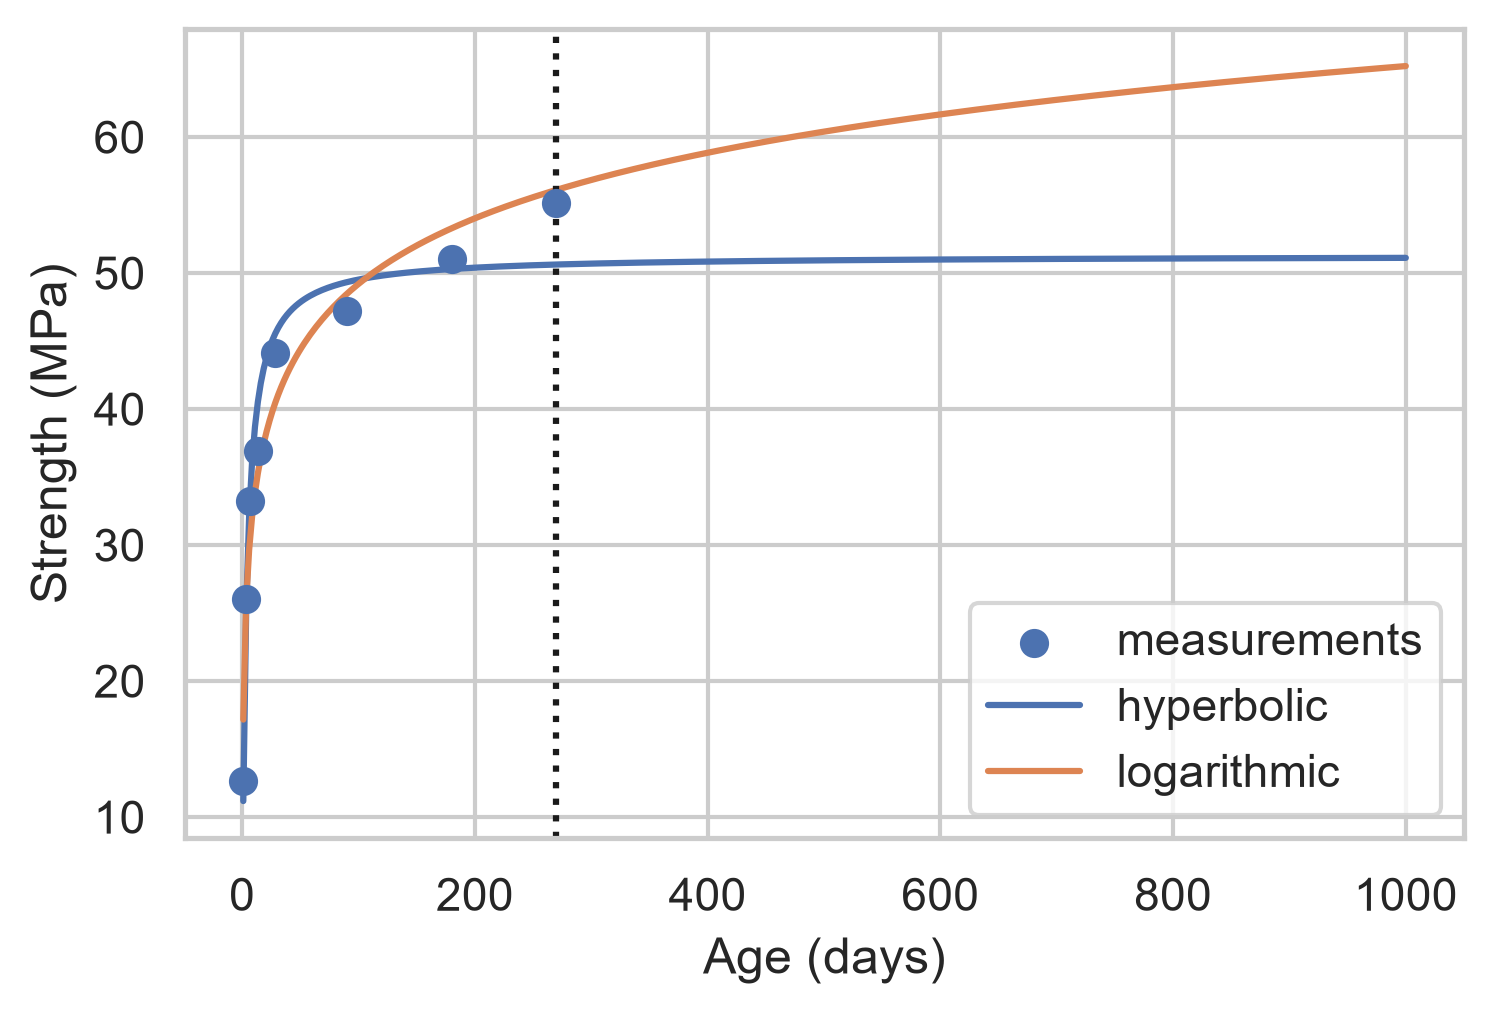
\includegraphics[keepaspectratio]{notebooks/05-regression-doe_files/figure-pdf/cell-17-output-1.png}}

Within the measured range both models can fit similarly well. Beyond it,
the logarithmic model grows without bound, while the hyperbolic model
approaches a final strength -- physically more plausible, since
hydration eventually stops. But neither model is validated beyond the
last measurement: long-term effects (e.g.~carbonation, drying) are not
in the data. Extrapolation relies on the model \emph{form}, not on data
-- and different plausible forms can give very different answers.

\end{tcolorbox}

\begin{tcolorbox}[enhanced jigsaw, colframe=quarto-callout-caution-color-frame, toprule=.15mm, rightrule=.15mm, title=\textcolor{quarto-callout-caution-color}{\faFire}\hspace{0.5em}{Solution to Exercise 6}, colbacktitle=quarto-callout-caution-color!10!white, left=2mm, titlerule=0mm, bottomtitle=1mm, toptitle=1mm, opacityback=0, bottomrule=.15mm, breakable, arc=.35mm, opacitybacktitle=0.6, colback=white, coltitle=black, leftrule=.75mm]

A \(2^4\) full factorial design needs \(2^4 = 16\) runs (32 with two
replicates). It estimates 4 main effects, 6 two-factor, 4 three-factor
and 1 four-factor interaction. A \textbf{fractional factorial design}
\(2^{4-1}\) uses only 8 runs, chosen such that the main effects remain
orthogonal. The price is \textbf{aliasing}: some effects can no longer
be distinguished -- in the \(2^{4-1}\) design with generator
\(D = ABC\), each main effect is aliased with a three-factor interaction
and the two-factor interactions are aliased in pairs. This is acceptable
when higher-order interactions are negligible, which is often the case
in screening experiments.

\begin{Shaded}
\begin{Highlighting}[]
\NormalTok{design4 }\OperatorTok{=}\NormalTok{ pd.DataFrame(}\BuiltInTok{list}\NormalTok{(itertools.product([}\OperatorTok{{-}}\DecValTok{1}\NormalTok{, }\DecValTok{1}\NormalTok{], repeat}\OperatorTok{=}\DecValTok{3}\NormalTok{)), columns}\OperatorTok{=}\BuiltInTok{list}\NormalTok{(}\StringTok{"ABC"}\NormalTok{))}
\NormalTok{design4[}\StringTok{"D"}\NormalTok{] }\OperatorTok{=}\NormalTok{ design4[}\StringTok{"A"}\NormalTok{] }\OperatorTok{*}\NormalTok{ design4[}\StringTok{"B"}\NormalTok{] }\OperatorTok{*}\NormalTok{ design4[}\StringTok{"C"}\NormalTok{]       }\CommentTok{\# generator D = ABC}
\NormalTok{design4}
\end{Highlighting}
\end{Shaded}

\begin{longtable}[]{@{}lllll@{}}
\toprule\noalign{}
& A & B & C & D \\
\midrule\noalign{}
\endhead
\bottomrule\noalign{}
\endlastfoot
0 & -1 & -1 & -1 & -1 \\
1 & -1 & -1 & 1 & 1 \\
2 & -1 & 1 & -1 & 1 \\
3 & -1 & 1 & 1 & -1 \\
4 & 1 & -1 & -1 & 1 \\
5 & 1 & -1 & 1 & -1 \\
6 & 1 & 1 & -1 & -1 \\
7 & 1 & 1 & 1 & 1 \\
\end{longtable}

\end{tcolorbox}

\chapter{Model Selection, Regularisation and Gaussian
Processes}\label{model-selection-regularisation-and-gaussian-processes}

A model that reproduces its training data perfectly is usually useless.
Given enough parameters, any model can pass through every data point --
including the noise. What we really want is a model that
\textbf{generalises}: that predicts well for new operating points, new
parts, next week's data. This chapter introduces the central idea of
machine learning: models must be judged on data they have not seen
during fitting.

We study how model complexity affects the prediction error, learn to
estimate this error honestly with cross-validation, and meet two ways to
control complexity: regularisation, which penalises large coefficients,
and Gaussian processes, a Bayesian approach that also tells us how
uncertain each prediction is.

\textbf{Scenario: a surrogate model instead of wind tunnel time}

An aerodynamics team is screening thousands of airfoil configurations
for a quiet fan blade. Each wind tunnel measurement costs half a day.
The team lead asks whether a data-driven model, trained on the existing
NASA measurements, could replace the tunnel for the screening stage. The
acoustics expert sets the requirement: the prediction error on
\emph{new} conditions must be below 2 dB (RMSE), otherwise the ranking
of configurations is unreliable.

\textbf{Your decision:} Which model, if any, do you release for the
screening?

\textbf{Learning goals.} After this chapter you can

\begin{itemize}
\tightlist
\item
  explain overfitting and the bias--variance trade-off,
\item
  evaluate models with train/test splits and k-fold cross-validation,
\item
  build preprocessing and model as a scikit-learn pipeline and avoid
  data leakage,
\item
  use Ridge and Lasso regression to control model complexity,
\item
  fit Gaussian process regression models and interpret their prediction
  uncertainty,
\item
  (extension) explain the idea of Bayesian optimisation for expensive
  experiments.
\end{itemize}

\textbf{Datasets in this chapter}

\begin{itemize}
\tightlist
\item
  \href{https://archive.ics.uci.edu/dataset/291/airfoil+self+noise}{Airfoil
  Self-Noise (UCI)}
\item
  \href{https://archive.ics.uci.edu/dataset/294/combined+cycle+power+plant}{Combined
  Cycle Power Plant (UCI)}
\end{itemize}

\section{Training error, test error and
overfitting}\label{training-error-test-error-and-overfitting}

Suppose the data are generated by \(y = f(x) + \varepsilon\) with an
unknown function \(f\) and noise \(\varepsilon\) with variance
\(\sigma^2\). We fit a model \(\hat f\) on a training set. Its error on
the \textbf{training data} is always optimistic: the model was tuned to
exactly these points. The relevant quantity is the expected error on
\textbf{new data} from the same process -- the \emph{generalisation
error} or \emph{test error}.

\begin{figure}[H]

\centering{

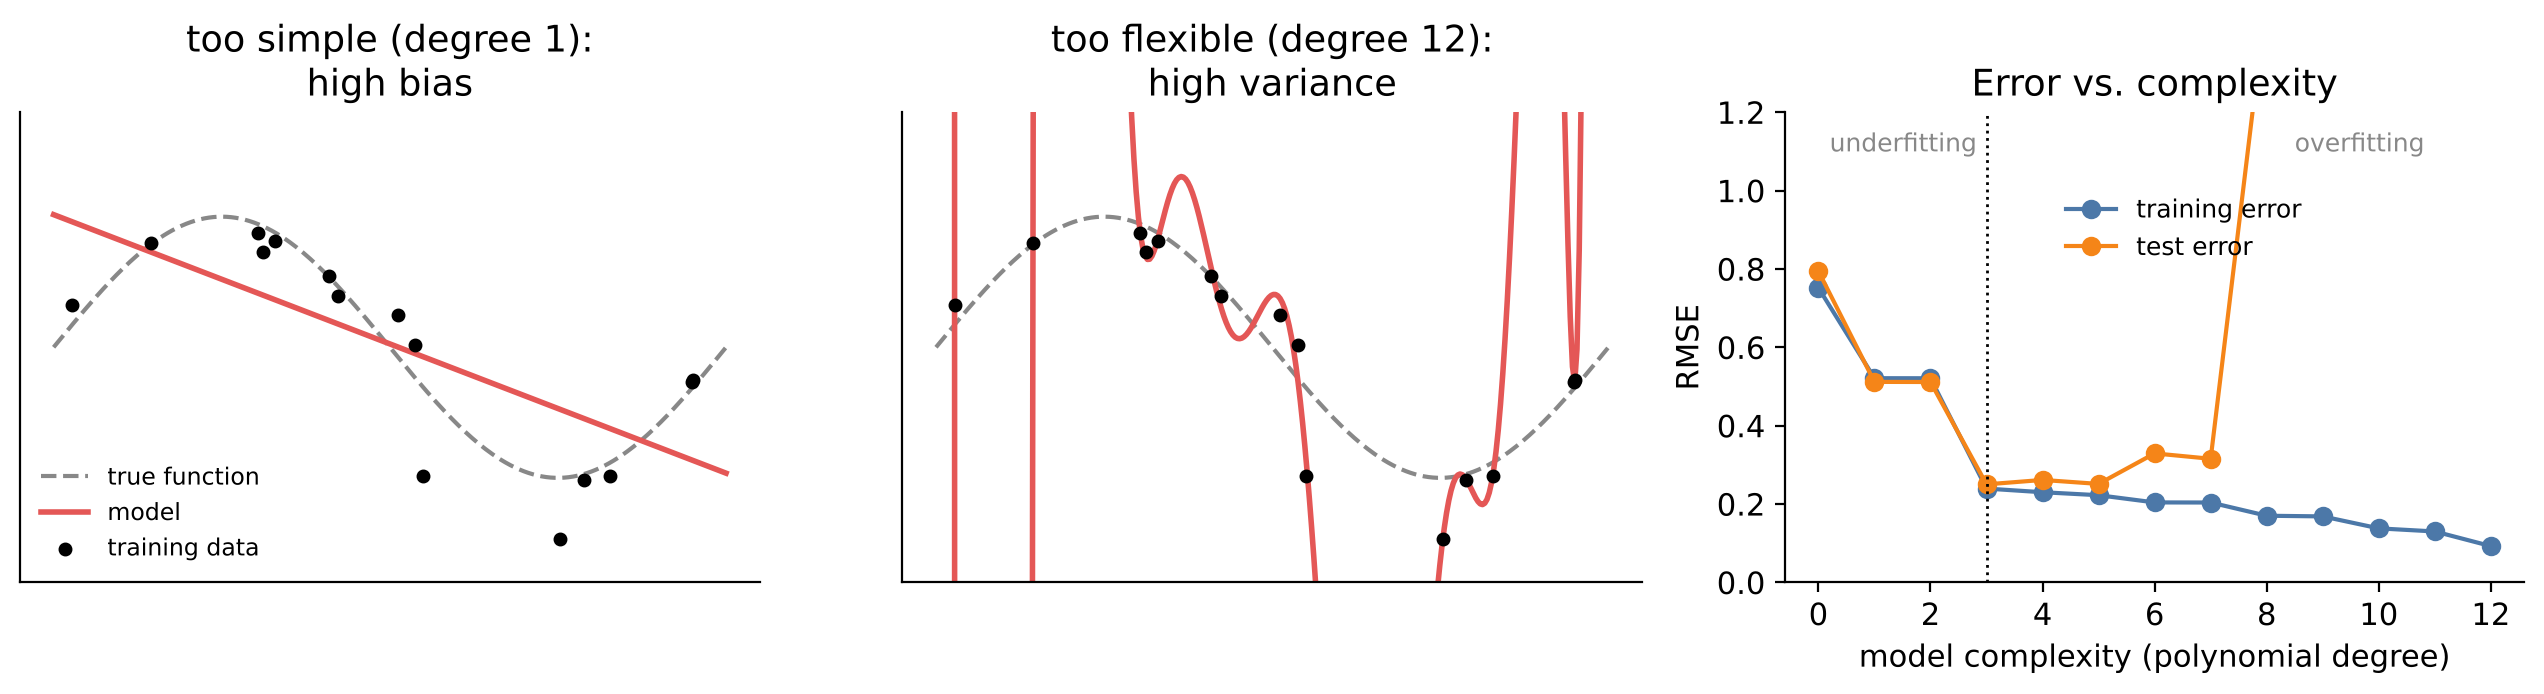
\includegraphics[width=1\linewidth,height=\textheight,keepaspectratio]{notebooks/images/overfitting.png}

}

\caption{\label{fig-overfitting}Under- and overfitting. A model that is
too simple (left) misses the structure; a model that is too flexible
(centre) follows the noise of the training data. The test error is
U-shaped in model complexity (right), while the training error keeps
decreasing.}

\end{figure}%

\begin{tcolorbox}[enhanced jigsaw, colframe=quarto-callout-important-color-frame, toprule=.15mm, rightrule=.15mm, title=\textcolor{quarto-callout-important-color}{\faExclamation}\hspace{0.5em}{Bias--variance decomposition}, colbacktitle=quarto-callout-important-color!10!white, left=2mm, titlerule=0mm, bottomtitle=1mm, toptitle=1mm, opacityback=0, bottomrule=.15mm, breakable, arc=.35mm, opacitybacktitle=0.6, colback=white, coltitle=black, leftrule=.75mm]

For squared error loss, the expected test error at a point \(x\)
decomposes into
\[E\big[(y - \hat f(x))^2\big] = \underbrace{\big(E[\hat f(x)] - f(x)\big)^2}_{\text{bias}^2} + \underbrace{\text{Var}\big(\hat f(x)\big)}_{\text{variance}} + \underbrace{\sigma^2}_{\text{irreducible noise}}.\]
Simple models have high \textbf{bias} (systematic error,
\emph{underfitting}); flexible models have high \textbf{variance} (they
change strongly with the training sample, \emph{overfitting}). The best
model balances both. The noise \(\sigma^2\) cannot be reduced by any
model.

\end{tcolorbox}

The practical consequence: \textbf{never judge a model by its training
error.} Set data aside for testing, or use cross-validation.

\section{Cross-validation}\label{cross-validation}

\begin{tcolorbox}[enhanced jigsaw, colframe=quarto-callout-note-color-frame, toprule=.15mm, rightrule=.15mm, title=\textcolor{quarto-callout-note-color}{\faInfo}\hspace{0.5em}{Definition: k-fold cross-validation}, colbacktitle=quarto-callout-note-color!10!white, left=2mm, titlerule=0mm, bottomtitle=1mm, toptitle=1mm, opacityback=0, bottomrule=.15mm, breakable, arc=.35mm, opacitybacktitle=0.6, colback=white, coltitle=black, leftrule=.75mm]

Split the data randomly into \(k\) parts (\emph{folds}) of equal size.
For each fold, train the model on the other \(k-1\) folds and compute
the error on the held-out fold. The \textbf{cross-validation error} is
the average over the \(k\) folds. Typical values are \(k = 5\) or
\(k = 10\).

\end{tcolorbox}

\begin{figure}[H]

\centering{

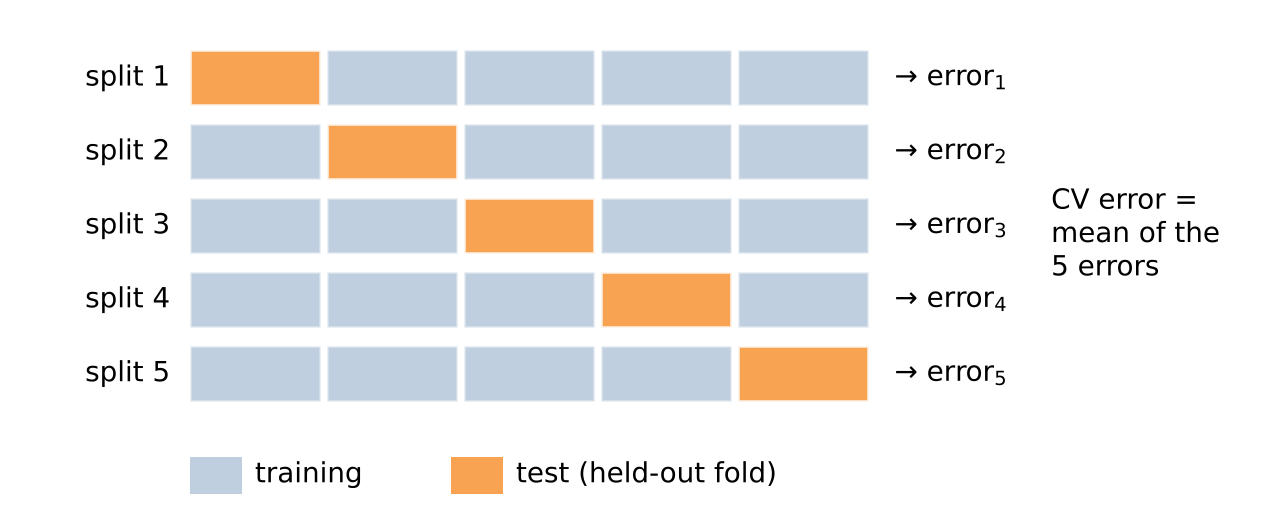
\includegraphics[width=0.8\linewidth,height=\textheight,keepaspectratio]{notebooks/images/kfold.png}

}

\caption{\label{fig-kfold}5-fold cross-validation: each observation is
used for testing exactly once and for training four times.}

\end{figure}%

Cross-validation uses the data efficiently and gives, besides the mean,
an idea of the variability of the error across folds. It is the standard
tool to \textbf{select} a model or a hyperparameter (polynomial degree,
regularisation strength). If the selected model's performance must be
reported, use a separate \textbf{test set} that was never touched during
selection -- otherwise the reported error is again optimistic.

\begin{tcolorbox}[enhanced jigsaw, colframe=quarto-callout-warning-color-frame, toprule=.15mm, rightrule=.15mm, title=\textcolor{quarto-callout-warning-color}{\faExclamationTriangle}\hspace{0.5em}{Pitfall: data leakage}, colbacktitle=quarto-callout-warning-color!10!white, left=2mm, titlerule=0mm, bottomtitle=1mm, toptitle=1mm, opacityback=0, bottomrule=.15mm, breakable, arc=.35mm, opacitybacktitle=0.6, colback=white, coltitle=black, leftrule=.75mm]

Any information from the test data that influences training makes the
test error too optimistic. Typical leaks: scaling or imputing with
statistics of the full dataset, selecting features by their correlation
with the target on all data, random splits of time series (Chapter 11),
or several rows of the same part/machine in both training and test set.
In scikit-learn, putting all preprocessing steps into a
\texttt{Pipeline} ensures that they are fitted inside each training fold
only.

\end{tcolorbox}

\section{Regularisation: Ridge and
Lasso}\label{regularisation-ridge-and-lasso}

Instead of choosing between few and many features, we can keep a
flexible model and penalise large coefficients:

\begin{tcolorbox}[enhanced jigsaw, colframe=quarto-callout-note-color-frame, toprule=.15mm, rightrule=.15mm, title=\textcolor{quarto-callout-note-color}{\faInfo}\hspace{0.5em}{Definition: Ridge and Lasso regression}, colbacktitle=quarto-callout-note-color!10!white, left=2mm, titlerule=0mm, bottomtitle=1mm, toptitle=1mm, opacityback=0, bottomrule=.15mm, breakable, arc=.35mm, opacitybacktitle=0.6, colback=white, coltitle=black, leftrule=.75mm]

\[\text{Ridge:}\quad \min_\beta \sum_i (y_i - x_i^\top\beta)^2 + \lambda \sum_j \beta_j^2, \qquad \text{Lasso:}\quad \min_\beta \sum_i (y_i - x_i^\top\beta)^2 + \lambda \sum_j |\beta_j|.\]
The hyperparameter \(\lambda \ge 0\) (in scikit-learn: \texttt{alpha})
controls the strength of the penalty: \(\lambda = 0\) gives ordinary
least squares, large \(\lambda\) shrinks all coefficients towards zero.

\end{tcolorbox}

Ridge shrinks coefficients smoothly and copes well with collinear
inputs. Lasso can set coefficients \textbf{exactly to zero} and thus
performs feature selection. Because the penalty depends on the size of
the coefficients, the inputs must be \textbf{standardised} first --
otherwise the penalty depends on the units. \(\lambda\) is chosen by
cross-validation (\texttt{RidgeCV}, \texttt{LassoCV}).

\begin{Shaded}
\begin{Highlighting}[]
\CommentTok{\# Setup: works locally and in Google Colab}
\ImportTok{import}\NormalTok{ importlib.util, subprocess, sys}
\ControlFlowTok{for}\NormalTok{ pkg }\KeywordTok{in}\NormalTok{ [}\StringTok{"ucimlrepo"}\NormalTok{]:}
    \ControlFlowTok{if}\NormalTok{ importlib.util.find\_spec(pkg) }\KeywordTok{is} \VariableTok{None}\NormalTok{:}
\NormalTok{        subprocess.run([sys.executable, }\StringTok{"{-}m"}\NormalTok{, }\StringTok{"pip"}\NormalTok{, }\StringTok{"install"}\NormalTok{, }\StringTok{"{-}q"}\NormalTok{, pkg], check}\OperatorTok{=}\VariableTok{True}\NormalTok{)}

\ImportTok{import}\NormalTok{ numpy }\ImportTok{as}\NormalTok{ np}
\ImportTok{import}\NormalTok{ pandas }\ImportTok{as}\NormalTok{ pd}
\ImportTok{import}\NormalTok{ matplotlib.pyplot }\ImportTok{as}\NormalTok{ plt}
\ImportTok{import}\NormalTok{ seaborn }\ImportTok{as}\NormalTok{ sns}

\NormalTok{sns.set\_theme(style}\OperatorTok{=}\StringTok{"whitegrid"}\NormalTok{)}
\end{Highlighting}
\end{Shaded}

\section{Live coding: airfoil
self-noise}\label{live-coding-airfoil-self-noise}

NASA measured the self-noise of airfoil sections (NACA 0012 profiles of
different chord lengths) in an anechoic wind tunnel. The noise is
generated by the interaction of the turbulent boundary layer with the
trailing edge -- a physically complex mechanism that is hard to model
from first principles. The dataset has 1,503 measurements:

\begin{longtable}[]{@{}lll@{}}
\toprule\noalign{}
Input & Meaning & Unit \\
\midrule\noalign{}
\endhead
\bottomrule\noalign{}
\endlastfoot
\texttt{frequency} & frequency & Hz \\
\texttt{angle} & angle of attack & deg \\
\texttt{chord} & chord length & m \\
\texttt{velocity} & free-stream velocity & m/s \\
\texttt{thickness} & suction side displacement thickness & m \\
\textbf{\texttt{spl}} (target) & scaled sound pressure level & dB \\
\end{longtable}

\begin{Shaded}
\begin{Highlighting}[]
\ImportTok{from}\NormalTok{ ucimlrepo }\ImportTok{import}\NormalTok{ fetch\_ucirepo}

\NormalTok{air }\OperatorTok{=}\NormalTok{ fetch\_ucirepo(}\BuiltInTok{id}\OperatorTok{=}\DecValTok{291}\NormalTok{)}
\NormalTok{X }\OperatorTok{=}\NormalTok{ air.data.features.copy()}
\NormalTok{X.columns }\OperatorTok{=}\NormalTok{ [}\StringTok{"frequency"}\NormalTok{, }\StringTok{"angle"}\NormalTok{, }\StringTok{"chord"}\NormalTok{, }\StringTok{"velocity"}\NormalTok{, }\StringTok{"thickness"}\NormalTok{]   }\CommentTok{\# Hz, deg, m, m/s, m}
\NormalTok{y }\OperatorTok{=}\NormalTok{ air.data.targets.iloc[:, }\DecValTok{0}\NormalTok{].rename(}\StringTok{"spl"}\NormalTok{)                           }\CommentTok{\# dB}
\NormalTok{X.describe().T.}\BuiltInTok{round}\NormalTok{(}\DecValTok{4}\NormalTok{)}
\end{Highlighting}
\end{Shaded}

\begin{longtable}[]{@{}lllllllll@{}}
\toprule\noalign{}
& count & mean & std & min & 25\% & 50\% & 75\% & max \\
\midrule\noalign{}
\endhead
\bottomrule\noalign{}
\endlastfoot
frequency & 1503.0 & 2886.3806 & 3152.5731 & 200.0000 & 800.0000 &
1600.0000 & 4000.0000 & 20000.0000 \\
angle & 1503.0 & 6.7823 & 5.9181 & 0.0000 & 2.0000 & 5.4000 & 9.9000 &
22.2000 \\
chord & 1503.0 & 0.1365 & 0.0935 & 0.0254 & 0.0508 & 0.1016 & 0.2286 &
0.3048 \\
velocity & 1503.0 & 50.8607 & 15.5728 & 31.7000 & 39.6000 & 39.6000 &
71.3000 & 71.3000 \\
thickness & 1503.0 & 0.0111 & 0.0132 & 0.0004 & 0.0025 & 0.0050 & 0.0156
& 0.0584 \\
\end{longtable}

\subsection{How complex should the model
be?}\label{how-complex-should-the-model-be}

We fit polynomial models of increasing degree -- with five inputs,
degree 6 already produces several hundred terms -- and compare training
and cross-validation errors.

\begin{Shaded}
\begin{Highlighting}[]
\ImportTok{from}\NormalTok{ sklearn.pipeline }\ImportTok{import}\NormalTok{ make\_pipeline}
\ImportTok{from}\NormalTok{ sklearn.preprocessing }\ImportTok{import}\NormalTok{ PolynomialFeatures, StandardScaler}
\ImportTok{from}\NormalTok{ sklearn.linear\_model }\ImportTok{import}\NormalTok{ LinearRegression, RidgeCV}
\ImportTok{from}\NormalTok{ sklearn.model\_selection }\ImportTok{import}\NormalTok{ KFold, cross\_validate}

\NormalTok{cv }\OperatorTok{=}\NormalTok{ KFold(n\_splits}\OperatorTok{=}\DecValTok{5}\NormalTok{, shuffle}\OperatorTok{=}\VariableTok{True}\NormalTok{, random\_state}\OperatorTok{=}\DecValTok{0}\NormalTok{)}
\NormalTok{rows }\OperatorTok{=}\NormalTok{ []}
\ControlFlowTok{for}\NormalTok{ degree }\KeywordTok{in} \BuiltInTok{range}\NormalTok{(}\DecValTok{1}\NormalTok{, }\DecValTok{7}\NormalTok{):}
\NormalTok{    pipe }\OperatorTok{=}\NormalTok{ make\_pipeline(PolynomialFeatures(degree), StandardScaler(), LinearRegression())}
\NormalTok{    res }\OperatorTok{=}\NormalTok{ cross\_validate(pipe, X, y, cv}\OperatorTok{=}\NormalTok{cv, scoring}\OperatorTok{=}\StringTok{"neg\_root\_mean\_squared\_error"}\NormalTok{,}
\NormalTok{                         return\_train\_score}\OperatorTok{=}\VariableTok{True}\NormalTok{)}
\NormalTok{    rows.append(\{}\StringTok{"degree"}\NormalTok{: degree, }\StringTok{"terms"}\NormalTok{: PolynomialFeatures(degree).fit(X).n\_output\_features\_,}
                 \StringTok{"train RMSE"}\NormalTok{: }\OperatorTok{{-}}\NormalTok{res[}\StringTok{"train\_score"}\NormalTok{].mean(), }\StringTok{"CV RMSE"}\NormalTok{: }\OperatorTok{{-}}\NormalTok{res[}\StringTok{"test\_score"}\NormalTok{].mean()\})}
\NormalTok{scores }\OperatorTok{=}\NormalTok{ pd.DataFrame(rows).set\_index(}\StringTok{"degree"}\NormalTok{)}
\NormalTok{ax }\OperatorTok{=}\NormalTok{ scores[[}\StringTok{"train RMSE"}\NormalTok{, }\StringTok{"CV RMSE"}\NormalTok{]].plot(marker}\OperatorTok{=}\StringTok{"o"}\NormalTok{)}
\NormalTok{ax.}\BuiltInTok{set}\NormalTok{(ylabel}\OperatorTok{=}\StringTok{"RMSE (dB)"}\NormalTok{, ylim}\OperatorTok{=}\NormalTok{(}\DecValTok{0}\NormalTok{, }\VariableTok{None}\NormalTok{))}
\NormalTok{plt.show()}
\NormalTok{scores.}\BuiltInTok{round}\NormalTok{(}\DecValTok{2}\NormalTok{)}
\end{Highlighting}
\end{Shaded}

\pandocbounded{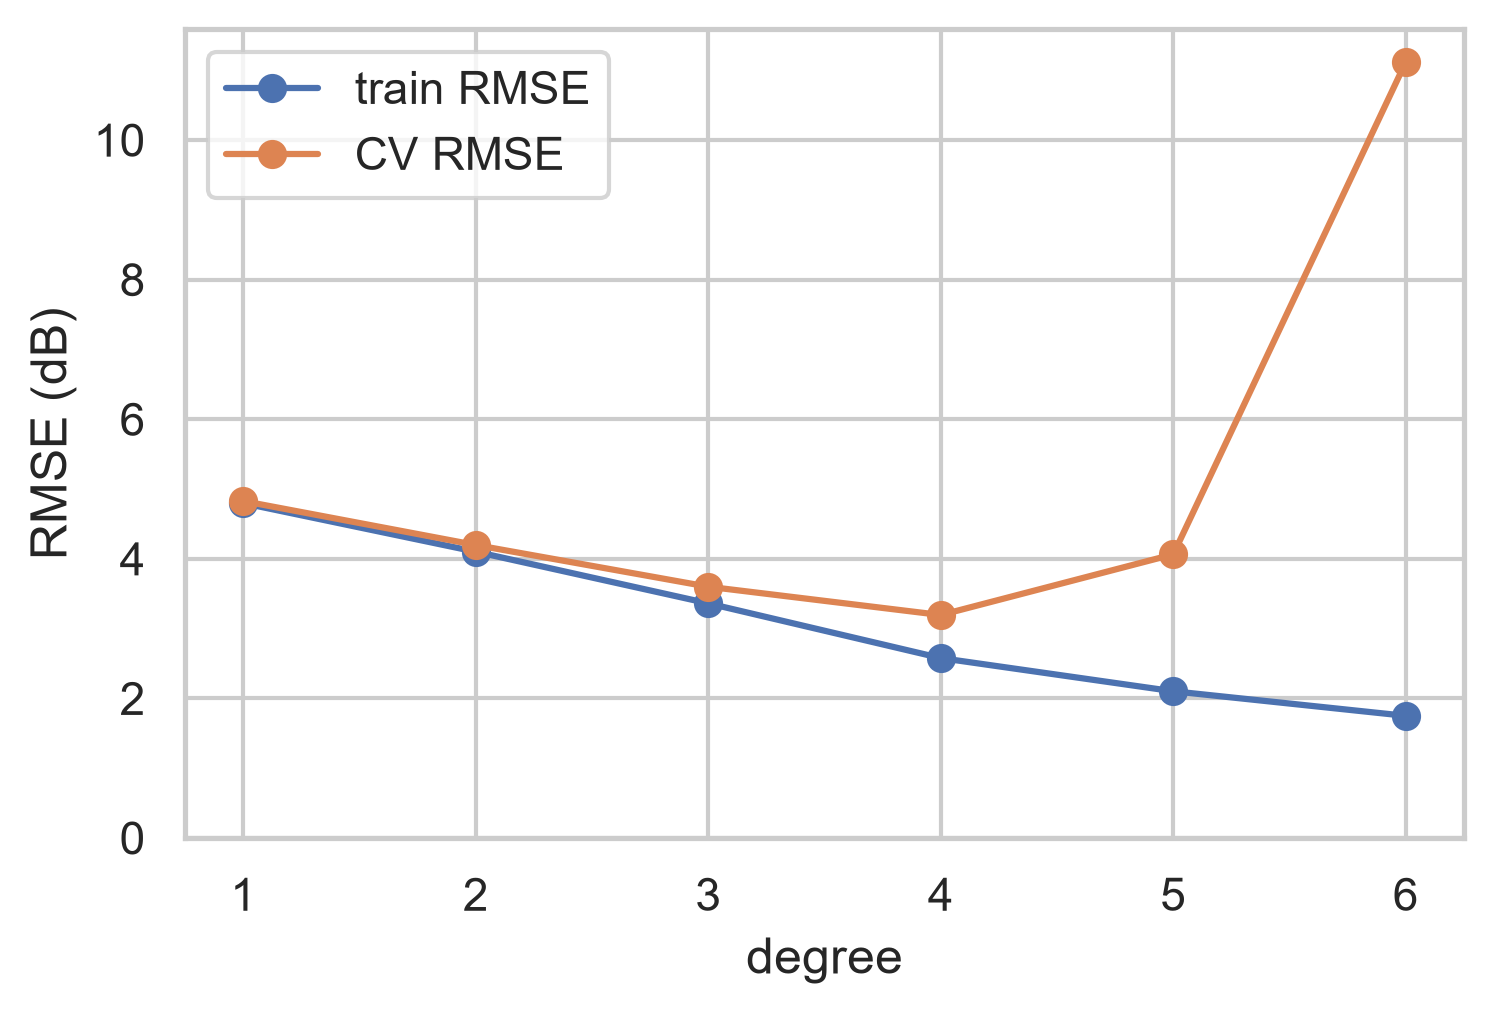
\includegraphics[keepaspectratio]{notebooks/06-model-selection_files/figure-pdf/cell-4-output-1.png}}

\begin{longtable}[]{@{}llll@{}}
\toprule\noalign{}
& terms & train RMSE & CV RMSE \\
degree & & & \\
\midrule\noalign{}
\endhead
\bottomrule\noalign{}
\endlastfoot
1 & 6 & 4.80 & 4.83 \\
2 & 21 & 4.10 & 4.20 \\
3 & 56 & 3.36 & 3.60 \\
4 & 126 & 2.58 & 3.19 \\
5 & 252 & 2.10 & 4.06 \\
6 & 462 & 1.75 & 11.12 \\
\end{longtable}

\textbf{Discussion.} The training error decreases steadily with the
degree -- more terms can always fit the training data better. The
cross-validation error first decreases (less bias) and eventually
increases again (more variance); its minimum indicates a good degree.
The growing gap between training and CV error is the signature of
overfitting. Note also the scale: a straight-line model leaves errors of
several dB, which matters for acoustic requirements.

\subsection{Regularisation in action}\label{regularisation-in-action}

Instead of picking the degree exactly, we can use a rich model and let
Ridge regression control its complexity. \texttt{RidgeCV} selects
\(\lambda\) by internal cross-validation; the outer cross-validation
evaluates the whole procedure.

\begin{Shaded}
\begin{Highlighting}[]
\NormalTok{ridge }\OperatorTok{=}\NormalTok{ make\_pipeline(PolynomialFeatures(}\DecValTok{5}\NormalTok{), StandardScaler(),}
\NormalTok{                      RidgeCV(alphas}\OperatorTok{=}\NormalTok{np.logspace(}\OperatorTok{{-}}\DecValTok{4}\NormalTok{, }\DecValTok{3}\NormalTok{, }\DecValTok{30}\NormalTok{)))}
\NormalTok{res\_ridge }\OperatorTok{=}\NormalTok{ cross\_validate(ridge, X, y, cv}\OperatorTok{=}\NormalTok{cv, scoring}\OperatorTok{=}\StringTok{"neg\_root\_mean\_squared\_error"}\NormalTok{)}
\BuiltInTok{print}\NormalTok{(}\SpecialStringTok{f"Ridge, degree 5: CV RMSE = }\SpecialCharTok{\{}\OperatorTok{{-}}\NormalTok{res\_ridge[}\StringTok{\textquotesingle{}test\_score\textquotesingle{}}\NormalTok{]}\SpecialCharTok{.}\NormalTok{mean()}\SpecialCharTok{:.2f\}}\SpecialStringTok{ dB"}\NormalTok{)}
\end{Highlighting}
\end{Shaded}

\begin{verbatim}
Ridge, degree 5: CV RMSE = 3.14 dB
\end{verbatim}

\begin{tcolorbox}[enhanced jigsaw, colframe=quarto-callout-tip-color-frame, toprule=.15mm, rightrule=.15mm, title=\textcolor{quarto-callout-tip-color}{\faLightbulb}\hspace{0.5em}{Engineering practice: nested model selection}, colbacktitle=quarto-callout-tip-color!10!white, left=2mm, titlerule=0mm, bottomtitle=1mm, toptitle=1mm, opacityback=0, bottomrule=.15mm, breakable, arc=.35mm, opacitybacktitle=0.6, colback=white, coltitle=black, leftrule=.75mm]

Here, cross-validation happens at two levels: \texttt{RidgeCV} chooses
\(\lambda\) on the training part of each outer fold, and the outer loop
measures how well the \emph{whole procedure} (including the choice of
\(\lambda\)) generalises. This \textbf{nested cross-validation} gives an
honest estimate. Choosing \(\lambda\) on the same folds used to report
the error would again be optimistic.

\end{tcolorbox}

\section{Gaussian process regression: predictions with
uncertainty}\label{gaussian-process-regression-predictions-with-uncertainty}

Polynomial and linear models assume a fixed functional form. A
\textbf{Gaussian process (GP)} places a probability distribution
directly over functions -- it is the Bayesian approach to regression.

\begin{tcolorbox}[enhanced jigsaw, colframe=quarto-callout-note-color-frame, toprule=.15mm, rightrule=.15mm, title=\textcolor{quarto-callout-note-color}{\faInfo}\hspace{0.5em}{Definition: Gaussian process}, colbacktitle=quarto-callout-note-color!10!white, left=2mm, titlerule=0mm, bottomtitle=1mm, toptitle=1mm, opacityback=0, bottomrule=.15mm, breakable, arc=.35mm, opacitybacktitle=0.6, colback=white, coltitle=black, leftrule=.75mm]

A Gaussian process is a collection of random variables \(f(x)\), any
finite number of which have a joint normal distribution. It is specified
by a mean function (often 0) and a \textbf{kernel} (covariance function)
\(\kappa(x, x')\) that states how strongly the function values at \(x\)
and \(x'\) are correlated. A common choice is the squared exponential
(RBF) kernel
\[\kappa(x, x') = \sigma_f^2 \exp\left(-\frac{\|x - x'\|^2}{2\ell^2}\right),\]
with signal variance \(\sigma_f^2\) and \textbf{length scale} \(\ell\)
(we write \(\kappa\) to avoid confusion with the \(k\) of k-fold
cross-validation): points closer than about \(\ell\) have similar
function values.

\end{tcolorbox}

Given training data, the GP posterior at a new point is again normal:
its \textbf{mean} is the prediction and its \textbf{standard deviation}
quantifies the uncertainty. Near the training points the uncertainty is
small, far away it grows back to the prior level. The kernel
hyperparameters and the noise level are fitted by maximising the
marginal likelihood -- no cross-validation needed.

\begin{figure}[H]

\centering{

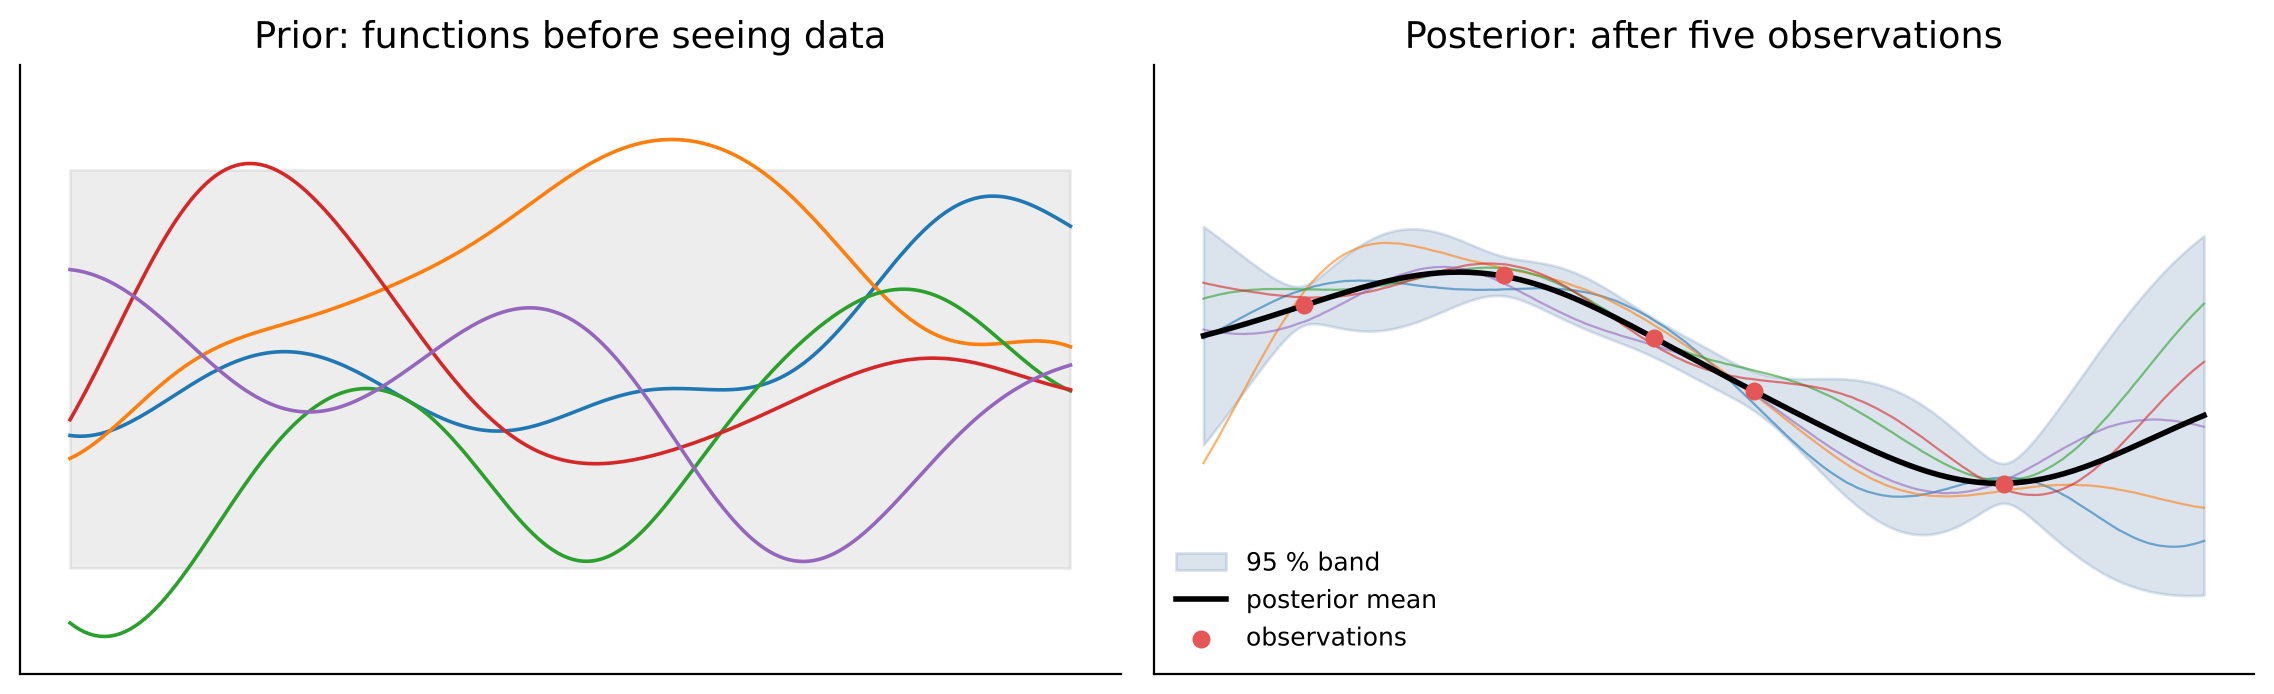
\includegraphics[width=1\linewidth,height=\textheight,keepaspectratio]{notebooks/images/gp-prior-posterior.png}

}

\caption{\label{fig-gp}A Gaussian process before and after observing
data. Left: functions drawn from the prior. Right: after five noisy
observations, the posterior mean interpolates the data and the
uncertainty band is narrow near the observations and wide in between and
outside.}

\end{figure}%

GPs are popular as \textbf{surrogate models} for expensive simulations
and experiments, where data are scarce and knowing the uncertainty
matters. Their limitation: the computational cost grows with \(n^3\), so
they suit datasets up to a few thousand points.

We first look at a one-dimensional example: the power output of the
combined cycle power plant as a function of ambient temperature, learned
from only 15 measurements.

\begin{Shaded}
\begin{Highlighting}[]
\ImportTok{from}\NormalTok{ sklearn.gaussian\_process }\ImportTok{import}\NormalTok{ GaussianProcessRegressor}
\ImportTok{from}\NormalTok{ sklearn.gaussian\_process.kernels }\ImportTok{import}\NormalTok{ RBF, WhiteKernel, ConstantKernel }\ImportTok{as}\NormalTok{ C}

\NormalTok{ccpp }\OperatorTok{=}\NormalTok{ fetch\_ucirepo(}\BuiltInTok{id}\OperatorTok{=}\DecValTok{294}\NormalTok{)}
\NormalTok{pp }\OperatorTok{=}\NormalTok{ pd.concat([ccpp.data.features, ccpp.data.targets], axis}\OperatorTok{=}\DecValTok{1}\NormalTok{)}
\NormalTok{few }\OperatorTok{=}\NormalTok{ pp.sample(}\DecValTok{15}\NormalTok{, random\_state}\OperatorTok{=}\DecValTok{1}\NormalTok{)}

\NormalTok{kernel }\OperatorTok{=}\NormalTok{ C(}\FloatTok{100.0}\NormalTok{) }\OperatorTok{*}\NormalTok{ RBF(length\_scale}\OperatorTok{=}\FloatTok{10.0}\NormalTok{) }\OperatorTok{+}\NormalTok{ WhiteKernel(noise\_level}\OperatorTok{=}\FloatTok{10.0}\NormalTok{)}
\NormalTok{gp }\OperatorTok{=}\NormalTok{ GaussianProcessRegressor(kernel}\OperatorTok{=}\NormalTok{kernel, normalize\_y}\OperatorTok{=}\VariableTok{True}\NormalTok{, random\_state}\OperatorTok{=}\DecValTok{0}\NormalTok{)}
\NormalTok{gp.fit(few[[}\StringTok{"AT"}\NormalTok{]], few[}\StringTok{"PE"}\NormalTok{])}
\BuiltInTok{print}\NormalTok{(}\StringTok{"Fitted kernel:"}\NormalTok{, gp.kernel\_)}

\NormalTok{T }\OperatorTok{=}\NormalTok{ np.linspace(}\OperatorTok{{-}}\DecValTok{5}\NormalTok{, }\DecValTok{45}\NormalTok{, }\DecValTok{300}\NormalTok{).reshape(}\OperatorTok{{-}}\DecValTok{1}\NormalTok{, }\DecValTok{1}\NormalTok{)}
\NormalTok{mean, std }\OperatorTok{=}\NormalTok{ gp.predict(pd.DataFrame(T, columns}\OperatorTok{=}\NormalTok{[}\StringTok{"AT"}\NormalTok{]), return\_std}\OperatorTok{=}\VariableTok{True}\NormalTok{)}
\NormalTok{plt.scatter(pp[}\StringTok{"AT"}\NormalTok{], pp[}\StringTok{"PE"}\NormalTok{], s}\OperatorTok{=}\DecValTok{2}\NormalTok{, c}\OperatorTok{=}\StringTok{"lightgray"}\NormalTok{, label}\OperatorTok{=}\StringTok{"all data (unknown to the model)"}\NormalTok{)}
\NormalTok{plt.scatter(few[}\StringTok{"AT"}\NormalTok{], few[}\StringTok{"PE"}\NormalTok{], c}\OperatorTok{=}\StringTok{"C3"}\NormalTok{, zorder}\OperatorTok{=}\DecValTok{3}\NormalTok{, label}\OperatorTok{=}\StringTok{"15 training points"}\NormalTok{)}
\NormalTok{plt.plot(T, mean, label}\OperatorTok{=}\StringTok{"GP mean"}\NormalTok{)}
\NormalTok{plt.fill\_between(T.ravel(), mean }\OperatorTok{{-}} \FloatTok{1.96} \OperatorTok{*}\NormalTok{ std, mean }\OperatorTok{+} \FloatTok{1.96} \OperatorTok{*}\NormalTok{ std, alpha}\OperatorTok{=}\FloatTok{0.3}\NormalTok{, label}\OperatorTok{=}\StringTok{"95 }\SpecialCharTok{\% i}\StringTok{nterval"}\NormalTok{)}
\NormalTok{plt.xlabel(}\StringTok{"Ambient temperature (°C)"}\NormalTok{)}\OperatorTok{;}\NormalTok{ plt.ylabel(}\StringTok{"Power output (MW)"}\NormalTok{)}\OperatorTok{;}\NormalTok{ plt.legend()}
\NormalTok{plt.show()}
\end{Highlighting}
\end{Shaded}

\begin{verbatim}
Fitted kernel: 2.27**2 * RBF(length_scale=29.5) + WhiteKernel(noise_level=0.118)
\end{verbatim}

\pandocbounded{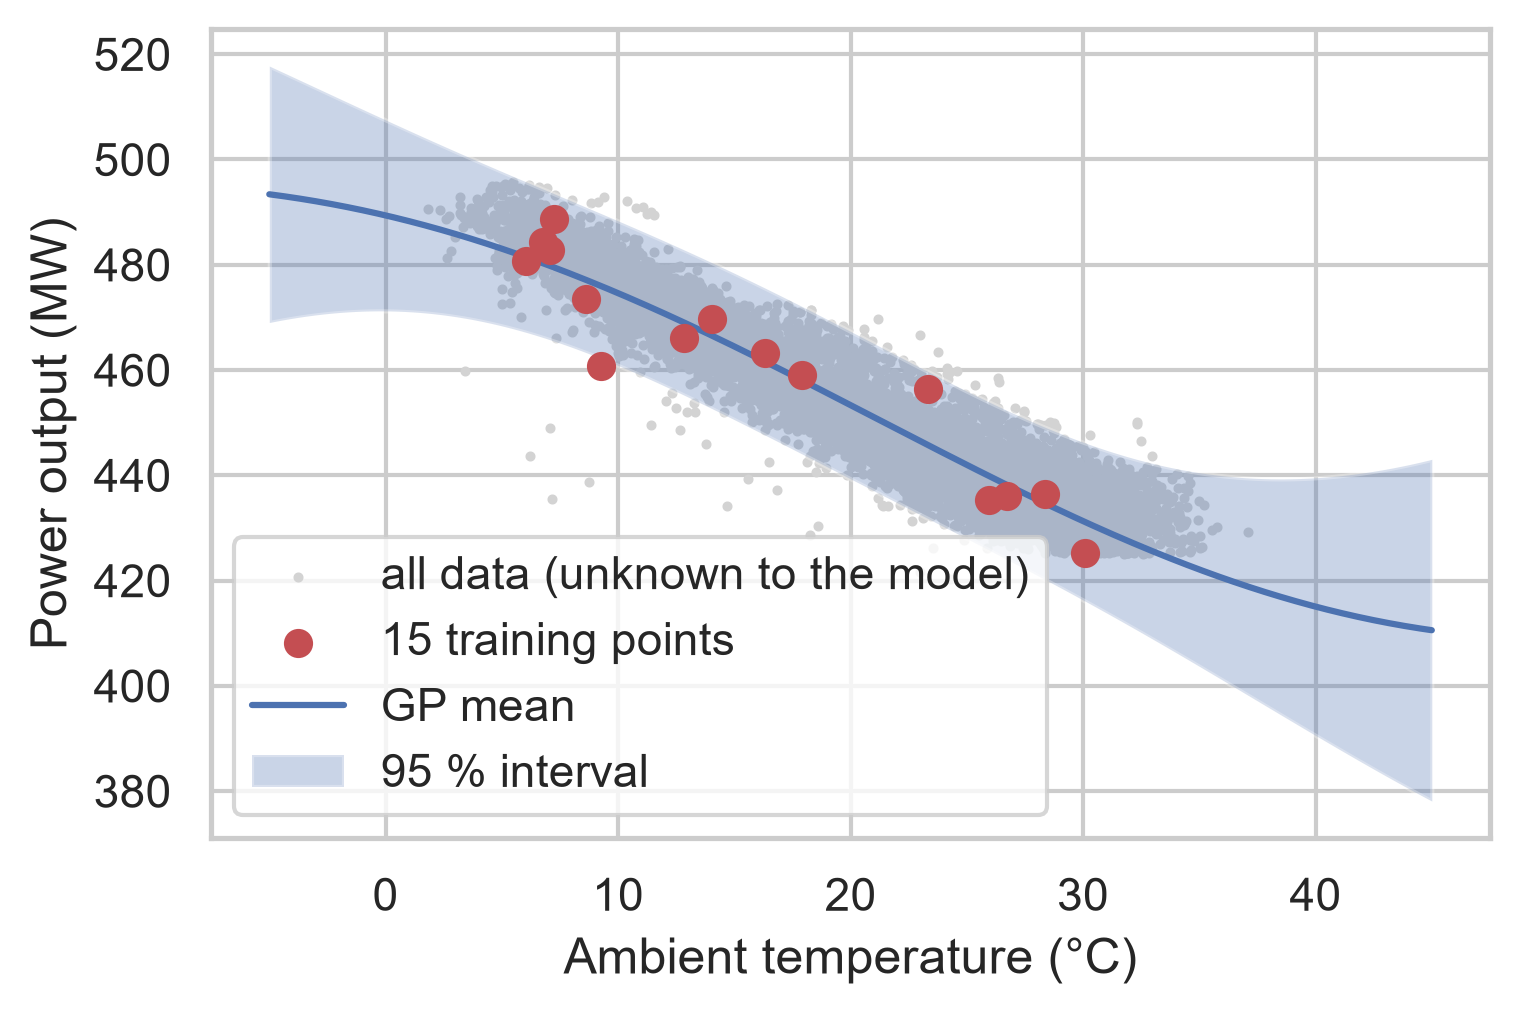
\includegraphics[keepaspectratio]{notebooks/06-model-selection_files/figure-pdf/cell-6-output-2.png}}

\textbf{Discussion.} With only 15 points, the GP recovers the almost
linear trend. The fitted \texttt{WhiteKernel} noise level estimates the
scatter of the individual measurements, the RBF length scale how quickly
the function can change. Outside the measured temperature range (below
the coldest and above the warmest training point), the band widens: the
model honestly reports that it does not know. A polynomial would
extrapolate with the same confidence everywhere.

\begin{Shaded}
\begin{Highlighting}[]
\CommentTok{\# GP on the full airfoil problem (5 inputs), compared with the polynomial ridge model}
\NormalTok{gp\_air }\OperatorTok{=}\NormalTok{ make\_pipeline(StandardScaler(), GaussianProcessRegressor(}
\NormalTok{    kernel}\OperatorTok{=}\NormalTok{C(}\FloatTok{1.0}\NormalTok{) }\OperatorTok{*}\NormalTok{ RBF(length\_scale}\OperatorTok{=}\NormalTok{np.ones(}\DecValTok{5}\NormalTok{)) }\OperatorTok{+}\NormalTok{ WhiteKernel(}\FloatTok{0.1}\NormalTok{), normalize\_y}\OperatorTok{=}\VariableTok{True}\NormalTok{))}
\NormalTok{res\_gp }\OperatorTok{=}\NormalTok{ cross\_validate(gp\_air, X, y, cv}\OperatorTok{=}\NormalTok{cv, scoring}\OperatorTok{=}\StringTok{"neg\_root\_mean\_squared\_error"}\NormalTok{)}
\BuiltInTok{print}\NormalTok{(}\SpecialStringTok{f"Gaussian process: CV RMSE = }\SpecialCharTok{\{}\OperatorTok{{-}}\NormalTok{res\_gp[}\StringTok{\textquotesingle{}test\_score\textquotesingle{}}\NormalTok{]}\SpecialCharTok{.}\NormalTok{mean()}\SpecialCharTok{:.2f\}}\SpecialStringTok{ dB"}\NormalTok{)}
\end{Highlighting}
\end{Shaded}

\begin{verbatim}
Gaussian process: CV RMSE = 1.89 dB
\end{verbatim}

Here we use one length scale per input (an \emph{anisotropic} or ARD
kernel). After fitting, a long length scale indicates that the output
changes slowly with that input -- a built-in measure of relevance.

\section{Back to the decision}\label{back-to-the-decision-5}

The requirement refers to new conditions, so we compare the
cross-validation errors -- never the training errors. Among the models
that meet the 2 dB requirement, we release the simplest one; if none
meets it, the tunnel cannot yet be replaced.

\begin{Shaded}
\begin{Highlighting}[]
\NormalTok{cv\_rmse }\OperatorTok{=}\NormalTok{ \{}
    \StringTok{"linear model"}\NormalTok{: scores.loc[}\DecValTok{1}\NormalTok{, }\StringTok{"CV RMSE"}\NormalTok{],}
    \SpecialStringTok{f"polynomial (degree }\SpecialCharTok{\{}\NormalTok{scores[}\StringTok{\textquotesingle{}CV RMSE\textquotesingle{}}\NormalTok{]}\SpecialCharTok{.}\NormalTok{idxmin()}\SpecialCharTok{\}}\SpecialStringTok{)"}\NormalTok{: scores[}\StringTok{"CV RMSE"}\NormalTok{].}\BuiltInTok{min}\NormalTok{(),}
    \StringTok{"polynomial degree 5 + Ridge"}\NormalTok{: }\OperatorTok{{-}}\NormalTok{res\_ridge[}\StringTok{"test\_score"}\NormalTok{].mean(),}
    \StringTok{"Gaussian process"}\NormalTok{: }\OperatorTok{{-}}\NormalTok{res\_gp[}\StringTok{"test\_score"}\NormalTok{].mean(),}
\NormalTok{\}}
\ControlFlowTok{for}\NormalTok{ name, e }\KeywordTok{in}\NormalTok{ cv\_rmse.items():}
    \BuiltInTok{print}\NormalTok{(}\SpecialStringTok{f"}\SpecialCharTok{\{}\NormalTok{name}\SpecialCharTok{:32s\}}\SpecialStringTok{ CV RMSE = }\SpecialCharTok{\{}\NormalTok{e}\SpecialCharTok{:.2f\}}\SpecialStringTok{ dB }\SpecialCharTok{\{}\StringTok{\textquotesingle{}✓\textquotesingle{}} \ControlFlowTok{if}\NormalTok{ e }\OperatorTok{\textless{}} \FloatTok{2.0} \ControlFlowTok{else} \StringTok{\textquotesingle{}✗\textquotesingle{}}\SpecialCharTok{\}}\SpecialStringTok{"}\NormalTok{)}
\NormalTok{ok }\OperatorTok{=}\NormalTok{ [name }\ControlFlowTok{for}\NormalTok{ name, e }\KeywordTok{in}\NormalTok{ cv\_rmse.items() }\ControlFlowTok{if}\NormalTok{ e }\OperatorTok{\textless{}} \FloatTok{2.0}\NormalTok{]}
\BuiltInTok{print}\NormalTok{(}\StringTok{"Decision:"}\NormalTok{, }\SpecialStringTok{f"release \textquotesingle{}}\SpecialCharTok{\{}\NormalTok{ok[}\DecValTok{0}\NormalTok{]}\SpecialCharTok{\}}\SpecialStringTok{\textquotesingle{} for the screening."} \ControlFlowTok{if}\NormalTok{ ok }\ControlFlowTok{else} \StringTok{"no model is accurate enough – keep using the tunnel."}\NormalTok{)}
\end{Highlighting}
\end{Shaded}

\begin{verbatim}
linear model                     CV RMSE = 4.83 dB ✗
polynomial (degree 4)            CV RMSE = 3.19 dB ✗
polynomial degree 5 + Ridge      CV RMSE = 3.14 dB ✗
Gaussian process                 CV RMSE = 1.89 dB ✓
Decision: release 'Gaussian process' for the screening.
\end{verbatim}

The models are listed from simple to complex, so the first model that
meets the requirement is released. Two caveats belong in the
recommendation: cross-validation estimates the error for conditions
\emph{similar} to the measured ones -- for configurations outside the
measured ranges (e.g.~larger chords or higher speeds) the error can be
much larger, and the Gaussian process at least signals this through its
uncertainty. And the best candidates of the screening should still be
confirmed in the tunnel.

\section{Extension: Bayesian optimisation -- design of experiments with
a
GP}\label{extension-bayesian-optimisation-design-of-experiments-with-a-gp}

\emph{Extension -- optional material, not required for the exam.}

When every experiment is expensive -- a test bench run, a CFD
simulation, a production trial -- we want to find the optimum with as
few runs as possible. \textbf{Bayesian optimisation} fits a GP to the
runs so far and chooses the next run where an \emph{acquisition
function} is largest. The popular \textbf{expected improvement} (EI) is

\[\text{EI}(x) = (\mu(x) - y^*)\,\Phi(z) + \sigma(x)\,\varphi(z), \qquad z = \frac{\mu(x) - y^*}{\sigma(x)},\]

where \(\mu(x)\) and \(\sigma(x)\) are the GP's predicted mean and
standard deviation at \(x\), \(y^*\) is the best result so far and
\(\Phi, \varphi\) are the standard normal CDF and PDF. EI is large where
the predicted mean is high (\emph{exploitation}) or the uncertainty is
large (\emph{exploration}).

The example uses a simulated ``experiment'': the yield of a process as a
function of temperature, which the algorithm does not know.

\begin{Shaded}
\begin{Highlighting}[]
\ImportTok{from}\NormalTok{ scipy.stats }\ImportTok{import}\NormalTok{ norm}

\KeywordTok{def}\NormalTok{ experiment(temp):                       }\CommentTok{\# unknown to the optimiser}
    \ControlFlowTok{return} \DecValTok{40} \OperatorTok{+} \DecValTok{45} \OperatorTok{*}\NormalTok{ np.exp(}\OperatorTok{{-}}\NormalTok{((temp }\OperatorTok{{-}} \DecValTok{172}\NormalTok{) }\OperatorTok{/} \DecValTok{25}\NormalTok{) }\OperatorTok{**} \DecValTok{2}\NormalTok{) }\OperatorTok{+} \DecValTok{5} \OperatorTok{*}\NormalTok{ np.sin(temp }\OperatorTok{/} \DecValTok{9}\NormalTok{)}

\NormalTok{grid }\OperatorTok{=}\NormalTok{ np.linspace(}\DecValTok{100}\NormalTok{, }\DecValTok{250}\NormalTok{, }\DecValTok{500}\NormalTok{).reshape(}\OperatorTok{{-}}\DecValTok{1}\NormalTok{, }\DecValTok{1}\NormalTok{)}
\NormalTok{X\_runs }\OperatorTok{=}\NormalTok{ np.array([[}\FloatTok{110.0}\NormalTok{], [}\FloatTok{180.0}\NormalTok{], [}\FloatTok{240.0}\NormalTok{]])            }\CommentTok{\# three initial runs}
\NormalTok{y\_runs }\OperatorTok{=}\NormalTok{ experiment(X\_runs.ravel())}

\NormalTok{fig, axes }\OperatorTok{=}\NormalTok{ plt.subplots(}\DecValTok{2}\NormalTok{, }\DecValTok{3}\NormalTok{, figsize}\OperatorTok{=}\NormalTok{(}\DecValTok{14}\NormalTok{, }\DecValTok{6}\NormalTok{), sharex}\OperatorTok{=}\VariableTok{True}\NormalTok{, sharey}\OperatorTok{=}\VariableTok{True}\NormalTok{)}
\ControlFlowTok{for}\NormalTok{ ax }\KeywordTok{in}\NormalTok{ axes.ravel():}
\NormalTok{    gp\_bo }\OperatorTok{=}\NormalTok{ GaussianProcessRegressor(C(}\FloatTok{1.0}\NormalTok{) }\OperatorTok{*}\NormalTok{ RBF(}\FloatTok{20.0}\NormalTok{), normalize\_y}\OperatorTok{=}\VariableTok{True}\NormalTok{, alpha}\OperatorTok{=}\FloatTok{1e{-}6}\NormalTok{)}
\NormalTok{    gp\_bo.fit(X\_runs, y\_runs)}
\NormalTok{    mu, sd }\OperatorTok{=}\NormalTok{ gp\_bo.predict(grid, return\_std}\OperatorTok{=}\VariableTok{True}\NormalTok{)}
\NormalTok{    best }\OperatorTok{=}\NormalTok{ y\_runs.}\BuiltInTok{max}\NormalTok{()}
\NormalTok{    z }\OperatorTok{=}\NormalTok{ (mu }\OperatorTok{{-}}\NormalTok{ best) }\OperatorTok{/}\NormalTok{ np.maximum(sd, }\FloatTok{1e{-}9}\NormalTok{)}
\NormalTok{    ei }\OperatorTok{=}\NormalTok{ (mu }\OperatorTok{{-}}\NormalTok{ best) }\OperatorTok{*}\NormalTok{ norm.cdf(z) }\OperatorTok{+}\NormalTok{ sd }\OperatorTok{*}\NormalTok{ norm.pdf(z)       }\CommentTok{\# expected improvement}
\NormalTok{    x\_next }\OperatorTok{=}\NormalTok{ grid[np.argmax(ei)]}

\NormalTok{    ax.plot(grid, experiment(grid.ravel()), }\StringTok{"k:"}\NormalTok{, lw}\OperatorTok{=}\DecValTok{1}\NormalTok{, label}\OperatorTok{=}\StringTok{"true (unknown)"}\NormalTok{)}
\NormalTok{    ax.plot(grid, mu, label}\OperatorTok{=}\StringTok{"GP mean"}\NormalTok{)}
\NormalTok{    ax.fill\_between(grid.ravel(), mu }\OperatorTok{{-}} \FloatTok{1.96} \OperatorTok{*}\NormalTok{ sd, mu }\OperatorTok{+} \FloatTok{1.96} \OperatorTok{*}\NormalTok{ sd, alpha}\OperatorTok{=}\FloatTok{0.25}\NormalTok{)}
\NormalTok{    ax.scatter(X\_runs, y\_runs, c}\OperatorTok{=}\StringTok{"C3"}\NormalTok{, zorder}\OperatorTok{=}\DecValTok{3}\NormalTok{, label}\OperatorTok{=}\StringTok{"runs"}\NormalTok{)}
\NormalTok{    ax.axvline(x\_next[}\DecValTok{0}\NormalTok{], c}\OperatorTok{=}\StringTok{"C2"}\NormalTok{, ls}\OperatorTok{=}\StringTok{"{-}{-}"}\NormalTok{, label}\OperatorTok{=}\StringTok{"next run"}\NormalTok{)}
\NormalTok{    ax.set\_title(}\SpecialStringTok{f"}\SpecialCharTok{\{}\BuiltInTok{len}\NormalTok{(y\_runs)}\SpecialCharTok{\}}\SpecialStringTok{ runs, best yield }\SpecialCharTok{\{}\NormalTok{best}\SpecialCharTok{:.1f\}}\SpecialStringTok{"}\NormalTok{)}

\NormalTok{    X\_runs }\OperatorTok{=}\NormalTok{ np.vstack([X\_runs, x\_next])}
\NormalTok{    y\_runs }\OperatorTok{=}\NormalTok{ np.append(y\_runs, experiment(x\_next[}\DecValTok{0}\NormalTok{]))}
\NormalTok{axes[}\DecValTok{0}\NormalTok{, }\DecValTok{0}\NormalTok{].legend(fontsize}\OperatorTok{=}\DecValTok{8}\NormalTok{)}
\NormalTok{fig.supxlabel(}\StringTok{"Temperature (°C)"}\NormalTok{)}\OperatorTok{;}\NormalTok{ fig.supylabel(}\StringTok{"Yield (\%)"}\NormalTok{)}
\NormalTok{plt.tight\_layout()}\OperatorTok{;}\NormalTok{ plt.show()}
\end{Highlighting}
\end{Shaded}

\pandocbounded{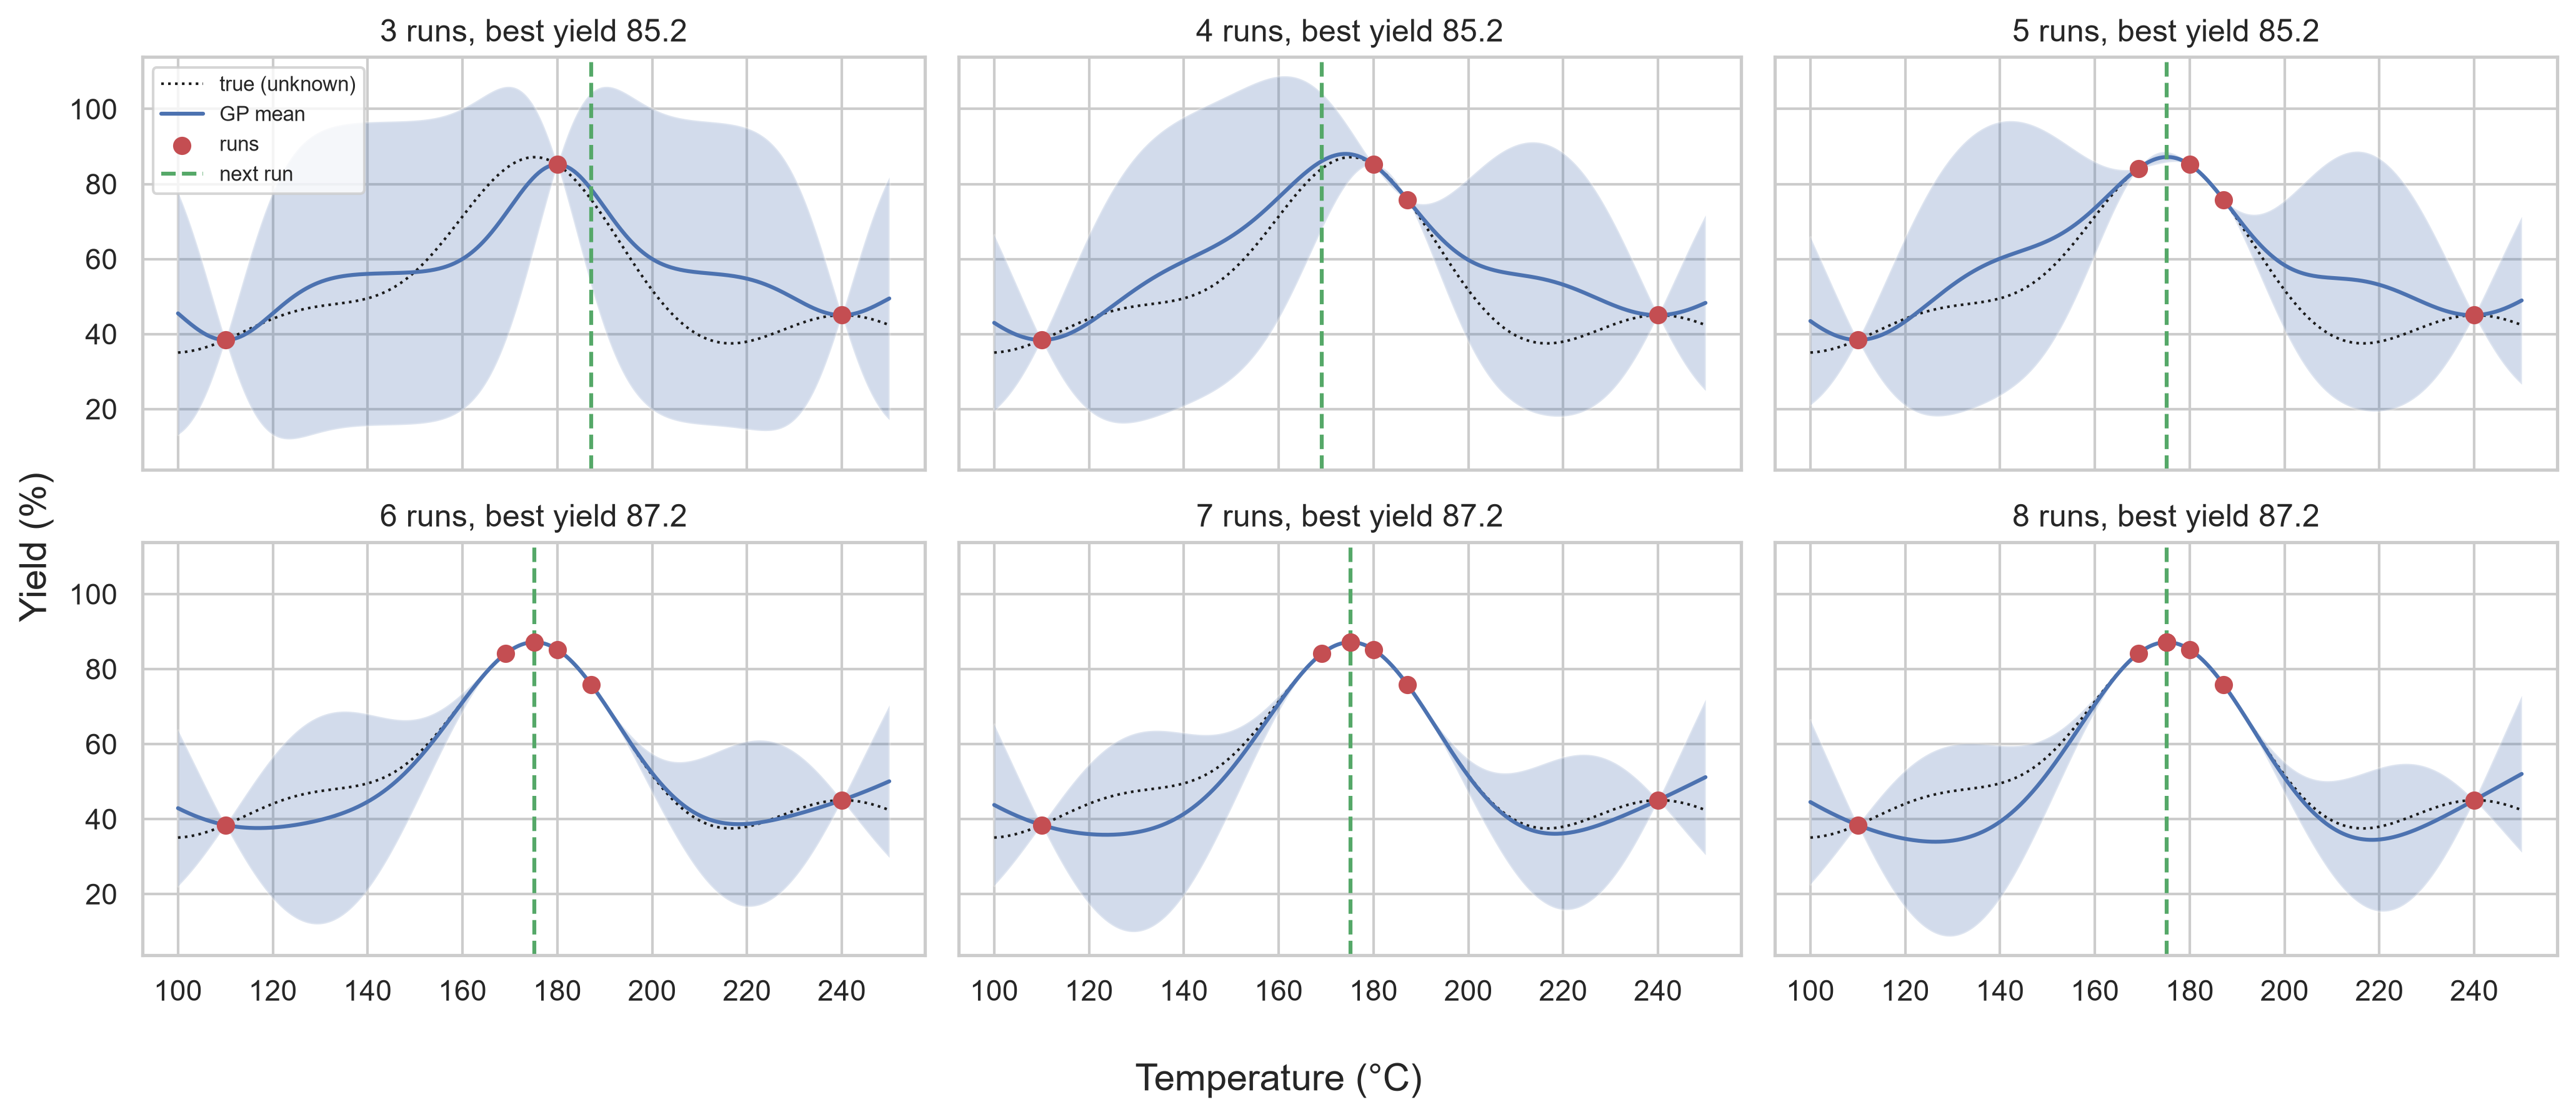
\includegraphics[keepaspectratio]{notebooks/06-model-selection_files/figure-pdf/cell-9-output-1.png}}

\textbf{Discussion.} After a few iterations the algorithm concentrates
its runs near the optimum, while regions that cannot contain a better
result are not explored further. Compared with a classical grid (Chapter
5), Bayesian optimisation adapts the design sequentially to the results
-- very efficient when runs are expensive and can be done one after
another. Once the optimum is found, EI becomes small everywhere and the
proposals cluster; in practice one stops when the expected improvement
falls below a threshold.

\begin{tcolorbox}[enhanced jigsaw, colframe=quarto-callout-important-color-frame, toprule=.15mm, rightrule=.15mm, title=\textcolor{quarto-callout-important-color}{\faExclamation}\hspace{0.5em}{Key takeaways}, colbacktitle=quarto-callout-important-color!10!white, left=2mm, titlerule=0mm, bottomtitle=1mm, toptitle=1mm, opacityback=0, bottomrule=.15mm, breakable, arc=.35mm, opacitybacktitle=0.6, colback=white, coltitle=black, leftrule=.75mm]

\begin{itemize}
\tightlist
\item
  The training error is optimistic; judge models by their error on
  unseen data.
\item
  The test error is U-shaped in model complexity: too simple → bias, too
  flexible → variance.
\item
  k-fold cross-validation selects models and hyperparameters;
  preprocessing belongs inside the pipeline.
\item
  Ridge and Lasso control complexity by penalising coefficients
  (standardise first!).
\item
  Gaussian processes give predictions with uncertainty -- valuable for
  small data and expensive experiments.
\end{itemize}

\end{tcolorbox}

\section{Exercises}\label{exercises-5}

\begin{enumerate}
\def\labelenumi{\arabic{enumi}.}
\tightlist
\item
  Repeat the degree study for the power plant data (\texttt{pp}, target
  \texttt{PE}). Why does the curve look so different from the airfoil
  case?
\item
  Why must the \texttt{StandardScaler} be part of the pipeline instead
  of being fitted on all data beforehand? Construct an example in which
  the difference becomes visible.
\item
  Plot predicted vs.~measured sound pressure level for the Ridge model,
  using \texttt{cross\_val\_predict}. In which range does the model
  fail?
\item
  GP: increase the number of training points from 15 to 50 and 200. How
  does the uncertainty band change? What happens outside the measured
  temperature range?
\item
  (Extension) Replace Ridge by \texttt{LassoCV} (degree 3). How many of
  the polynomial features survive?
\item
  (Extension) Bayesian optimisation: start with a different set of three
  runs. Does the algorithm still find the optimum? Compare with a
  regular grid of the same number of runs.
\end{enumerate}

\subsection{Solutions}\label{solutions-5}

\begin{tcolorbox}[enhanced jigsaw, colframe=quarto-callout-caution-color-frame, toprule=.15mm, rightrule=.15mm, title=\textcolor{quarto-callout-caution-color}{\faFire}\hspace{0.5em}{Solution to Exercise 1}, colbacktitle=quarto-callout-caution-color!10!white, left=2mm, titlerule=0mm, bottomtitle=1mm, toptitle=1mm, opacityback=0, bottomrule=.15mm, breakable, arc=.35mm, opacitybacktitle=0.6, colback=white, coltitle=black, leftrule=.75mm]

\begin{Shaded}
\begin{Highlighting}[]
\NormalTok{X\_pp, y\_pp }\OperatorTok{=}\NormalTok{ pp[[}\StringTok{"AT"}\NormalTok{, }\StringTok{"V"}\NormalTok{, }\StringTok{"AP"}\NormalTok{, }\StringTok{"RH"}\NormalTok{]], pp[}\StringTok{"PE"}\NormalTok{]}
\NormalTok{rows }\OperatorTok{=}\NormalTok{ []}
\ControlFlowTok{for}\NormalTok{ degree }\KeywordTok{in} \BuiltInTok{range}\NormalTok{(}\DecValTok{1}\NormalTok{, }\DecValTok{6}\NormalTok{):}
\NormalTok{    pipe }\OperatorTok{=}\NormalTok{ make\_pipeline(PolynomialFeatures(degree), StandardScaler(), LinearRegression())}
\NormalTok{    res }\OperatorTok{=}\NormalTok{ cross\_validate(pipe, X\_pp, y\_pp, cv}\OperatorTok{=}\NormalTok{cv, scoring}\OperatorTok{=}\StringTok{"neg\_root\_mean\_squared\_error"}\NormalTok{,}
\NormalTok{                         return\_train\_score}\OperatorTok{=}\VariableTok{True}\NormalTok{)}
\NormalTok{    rows.append(\{}\StringTok{"degree"}\NormalTok{: degree, }\StringTok{"train RMSE"}\NormalTok{: }\OperatorTok{{-}}\NormalTok{res[}\StringTok{"train\_score"}\NormalTok{].mean(),}
                 \StringTok{"CV RMSE"}\NormalTok{: }\OperatorTok{{-}}\NormalTok{res[}\StringTok{"test\_score"}\NormalTok{].mean()\})}
\NormalTok{pd.DataFrame(rows).set\_index(}\StringTok{"degree"}\NormalTok{).}\BuiltInTok{round}\NormalTok{(}\DecValTok{3}\NormalTok{)}
\end{Highlighting}
\end{Shaded}

\begin{longtable}[]{@{}lll@{}}
\toprule\noalign{}
& train RMSE & CV RMSE \\
degree & & \\
\midrule\noalign{}
\endhead
\bottomrule\noalign{}
\endlastfoot
1 & 4.557 & 4.559 \\
2 & 4.254 & 4.260 \\
3 & 4.149 & 4.162 \\
4 & 4.088 & 4.118 \\
5 & 4.030 & 4.073 \\
\end{longtable}

The power plant relationship is nearly linear, there are only four
inputs and almost 10,000 observations. Higher degrees improve the fit
only slightly, and training and CV errors stay close together -- with
this much data relative to the number of parameters, overfitting hardly
occurs. The remaining error is dominated by the irreducible noise. The
airfoil problem is more nonlinear and has six times less data, so
flexibility helps first and then overfits.

\end{tcolorbox}

\begin{tcolorbox}[enhanced jigsaw, colframe=quarto-callout-caution-color-frame, toprule=.15mm, rightrule=.15mm, title=\textcolor{quarto-callout-caution-color}{\faFire}\hspace{0.5em}{Solution to Exercise 2}, colbacktitle=quarto-callout-caution-color!10!white, left=2mm, titlerule=0mm, bottomtitle=1mm, toptitle=1mm, opacityback=0, bottomrule=.15mm, breakable, arc=.35mm, opacitybacktitle=0.6, colback=white, coltitle=black, leftrule=.75mm]

Fitting the scaler on all data uses the means and standard deviations of
the test folds -- a (here mild) form of leakage. The effect is small for
scaling with many observations but becomes large for steps that use the
target, e.g.~selecting the features most correlated with \(y\) before
cross-validation:

\begin{Shaded}
\begin{Highlighting}[]
\ImportTok{from}\NormalTok{ sklearn.feature\_selection }\ImportTok{import}\NormalTok{ SelectKBest, f\_regression}

\NormalTok{rng }\OperatorTok{=}\NormalTok{ np.random.default\_rng(}\DecValTok{0}\NormalTok{)}
\NormalTok{noise }\OperatorTok{=}\NormalTok{ pd.DataFrame(rng.normal(size}\OperatorTok{=}\NormalTok{(}\DecValTok{100}\NormalTok{, }\DecValTok{2000}\NormalTok{)))          }\CommentTok{\# pure noise features}
\NormalTok{target }\OperatorTok{=}\NormalTok{ pd.Series(rng.normal(size}\OperatorTok{=}\DecValTok{100}\NormalTok{))                     }\CommentTok{\# unrelated target}

\NormalTok{leaky\_X }\OperatorTok{=}\NormalTok{ SelectKBest(f\_regression, k}\OperatorTok{=}\DecValTok{20}\NormalTok{).fit\_transform(noise, target)   }\CommentTok{\# selection on ALL data}
\NormalTok{leaky }\OperatorTok{=}\NormalTok{ cross\_validate(LinearRegression(), leaky\_X, target, cv}\OperatorTok{=}\NormalTok{cv, scoring}\OperatorTok{=}\StringTok{"r2"}\NormalTok{)[}\StringTok{"test\_score"}\NormalTok{].mean()}
\NormalTok{proper }\OperatorTok{=}\NormalTok{ cross\_validate(make\_pipeline(SelectKBest(f\_regression, k}\OperatorTok{=}\DecValTok{20}\NormalTok{), LinearRegression()),}
\NormalTok{                        noise, target, cv}\OperatorTok{=}\NormalTok{cv, scoring}\OperatorTok{=}\StringTok{"r2"}\NormalTok{)[}\StringTok{"test\_score"}\NormalTok{].mean()}
\BuiltInTok{print}\NormalTok{(}\SpecialStringTok{f"CV R² with leaky selection: }\SpecialCharTok{\{}\NormalTok{leaky}\SpecialCharTok{:.2f\}}\SpecialStringTok{,  inside the pipeline: }\SpecialCharTok{\{}\NormalTok{proper}\SpecialCharTok{:.2f\}}\SpecialStringTok{"}\NormalTok{)}
\end{Highlighting}
\end{Shaded}

\begin{verbatim}
CV R² with leaky selection: 0.47,  inside the pipeline: -0.32
\end{verbatim}

With selection outside the pipeline, the ``model'' appears to predict
pure noise; inside the pipeline the CV R² is correctly around zero or
negative.

\end{tcolorbox}

\begin{tcolorbox}[enhanced jigsaw, colframe=quarto-callout-caution-color-frame, toprule=.15mm, rightrule=.15mm, title=\textcolor{quarto-callout-caution-color}{\faFire}\hspace{0.5em}{Solution to Exercise 3}, colbacktitle=quarto-callout-caution-color!10!white, left=2mm, titlerule=0mm, bottomtitle=1mm, toptitle=1mm, opacityback=0, bottomrule=.15mm, breakable, arc=.35mm, opacitybacktitle=0.6, colback=white, coltitle=black, leftrule=.75mm]

\begin{Shaded}
\begin{Highlighting}[]
\ImportTok{from}\NormalTok{ sklearn.model\_selection }\ImportTok{import}\NormalTok{ cross\_val\_predict}

\NormalTok{y\_hat }\OperatorTok{=}\NormalTok{ cross\_val\_predict(ridge, X, y, cv}\OperatorTok{=}\NormalTok{cv)}
\NormalTok{plt.scatter(y, y\_hat, s}\OperatorTok{=}\DecValTok{8}\NormalTok{, alpha}\OperatorTok{=}\FloatTok{0.5}\NormalTok{)}
\NormalTok{lims }\OperatorTok{=}\NormalTok{ [y.}\BuiltInTok{min}\NormalTok{(), y.}\BuiltInTok{max}\NormalTok{()]}
\NormalTok{plt.plot(lims, lims, }\StringTok{"k{-}{-}"}\NormalTok{)}
\NormalTok{plt.xlabel(}\StringTok{"Measured SPL (dB)"}\NormalTok{)}\OperatorTok{;}\NormalTok{ plt.ylabel(}\StringTok{"Predicted SPL (dB)"}\NormalTok{)}
\NormalTok{plt.show()}
\end{Highlighting}
\end{Shaded}

\pandocbounded{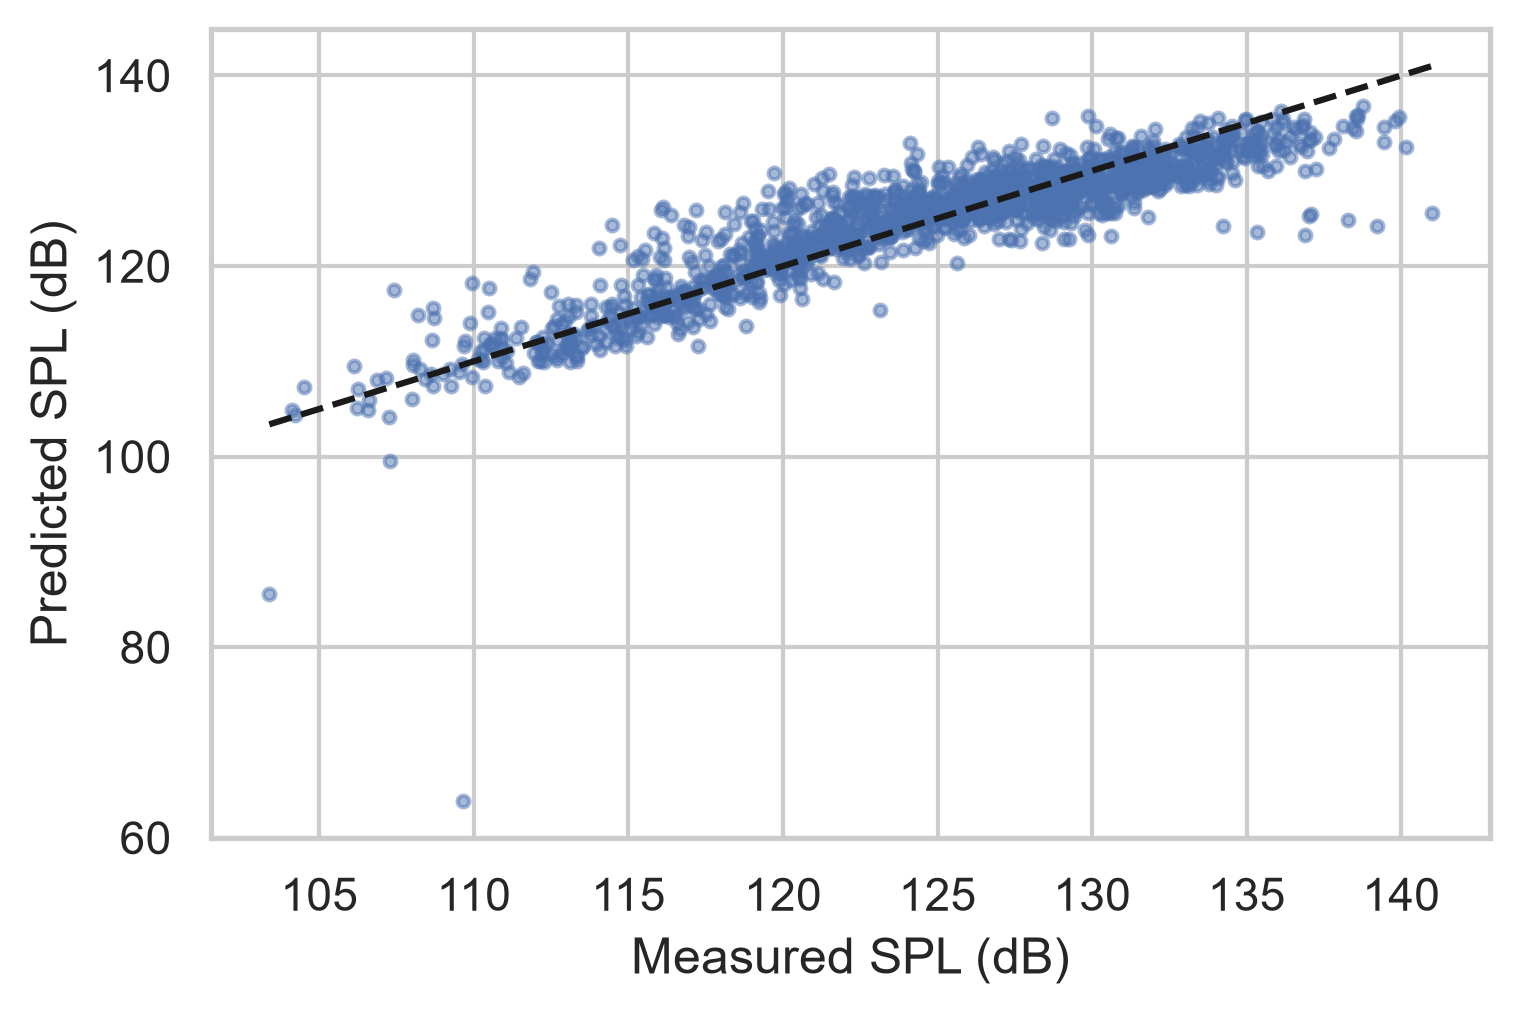
\includegraphics[keepaspectratio]{notebooks/06-model-selection_files/figure-pdf/cell-12-output-1.png}}

\texttt{cross\_val\_predict} returns for each observation the prediction
of the model that did \emph{not} see it during training. Deviations are
typically largest at the extremes -- the quietest and loudest conditions
are underrepresented, and the model shrinks predictions towards the mean
(a typical effect of regularisation). Plotting the residuals against
frequency shows that some frequency ranges are captured less well than
others.

\end{tcolorbox}

\begin{tcolorbox}[enhanced jigsaw, colframe=quarto-callout-caution-color-frame, toprule=.15mm, rightrule=.15mm, title=\textcolor{quarto-callout-caution-color}{\faFire}\hspace{0.5em}{Solution to Exercise 4}, colbacktitle=quarto-callout-caution-color!10!white, left=2mm, titlerule=0mm, bottomtitle=1mm, toptitle=1mm, opacityback=0, bottomrule=.15mm, breakable, arc=.35mm, opacitybacktitle=0.6, colback=white, coltitle=black, leftrule=.75mm]

\begin{Shaded}
\begin{Highlighting}[]
\NormalTok{fig, axes }\OperatorTok{=}\NormalTok{ plt.subplots(}\DecValTok{1}\NormalTok{, }\DecValTok{3}\NormalTok{, figsize}\OperatorTok{=}\NormalTok{(}\DecValTok{15}\NormalTok{, }\DecValTok{4}\NormalTok{), sharey}\OperatorTok{=}\VariableTok{True}\NormalTok{)}
\ControlFlowTok{for}\NormalTok{ ax, n\_train }\KeywordTok{in} \BuiltInTok{zip}\NormalTok{(axes, [}\DecValTok{15}\NormalTok{, }\DecValTok{50}\NormalTok{, }\DecValTok{200}\NormalTok{]):}
\NormalTok{    sub }\OperatorTok{=}\NormalTok{ pp.sample(n\_train, random\_state}\OperatorTok{=}\DecValTok{1}\NormalTok{)}
\NormalTok{    g }\OperatorTok{=}\NormalTok{ GaussianProcessRegressor(kernel}\OperatorTok{=}\NormalTok{kernel, normalize\_y}\OperatorTok{=}\VariableTok{True}\NormalTok{, random\_state}\OperatorTok{=}\DecValTok{0}\NormalTok{).fit(sub[[}\StringTok{"AT"}\NormalTok{]], sub[}\StringTok{"PE"}\NormalTok{])}
\NormalTok{    m, s }\OperatorTok{=}\NormalTok{ g.predict(pd.DataFrame(T, columns}\OperatorTok{=}\NormalTok{[}\StringTok{"AT"}\NormalTok{]), return\_std}\OperatorTok{=}\VariableTok{True}\NormalTok{)}
\NormalTok{    ax.scatter(sub[}\StringTok{"AT"}\NormalTok{], sub[}\StringTok{"PE"}\NormalTok{], s}\OperatorTok{=}\DecValTok{8}\NormalTok{, c}\OperatorTok{=}\StringTok{"C3"}\NormalTok{)}
\NormalTok{    ax.plot(T, m)}\OperatorTok{;}\NormalTok{ ax.fill\_between(T.ravel(), m }\OperatorTok{{-}} \FloatTok{1.96} \OperatorTok{*}\NormalTok{ s, m }\OperatorTok{+} \FloatTok{1.96} \OperatorTok{*}\NormalTok{ s, alpha}\OperatorTok{=}\FloatTok{0.3}\NormalTok{)}
\NormalTok{    ax.}\BuiltInTok{set}\NormalTok{(title}\OperatorTok{=}\SpecialStringTok{f"n = }\SpecialCharTok{\{}\NormalTok{n\_train}\SpecialCharTok{\}}\SpecialStringTok{"}\NormalTok{, xlabel}\OperatorTok{=}\StringTok{"AT (°C)"}\NormalTok{)}
\NormalTok{axes[}\DecValTok{0}\NormalTok{].set\_ylabel(}\StringTok{"PE (MW)"}\NormalTok{)}
\NormalTok{plt.tight\_layout()}\OperatorTok{;}\NormalTok{ plt.show()}
\end{Highlighting}
\end{Shaded}

\pandocbounded{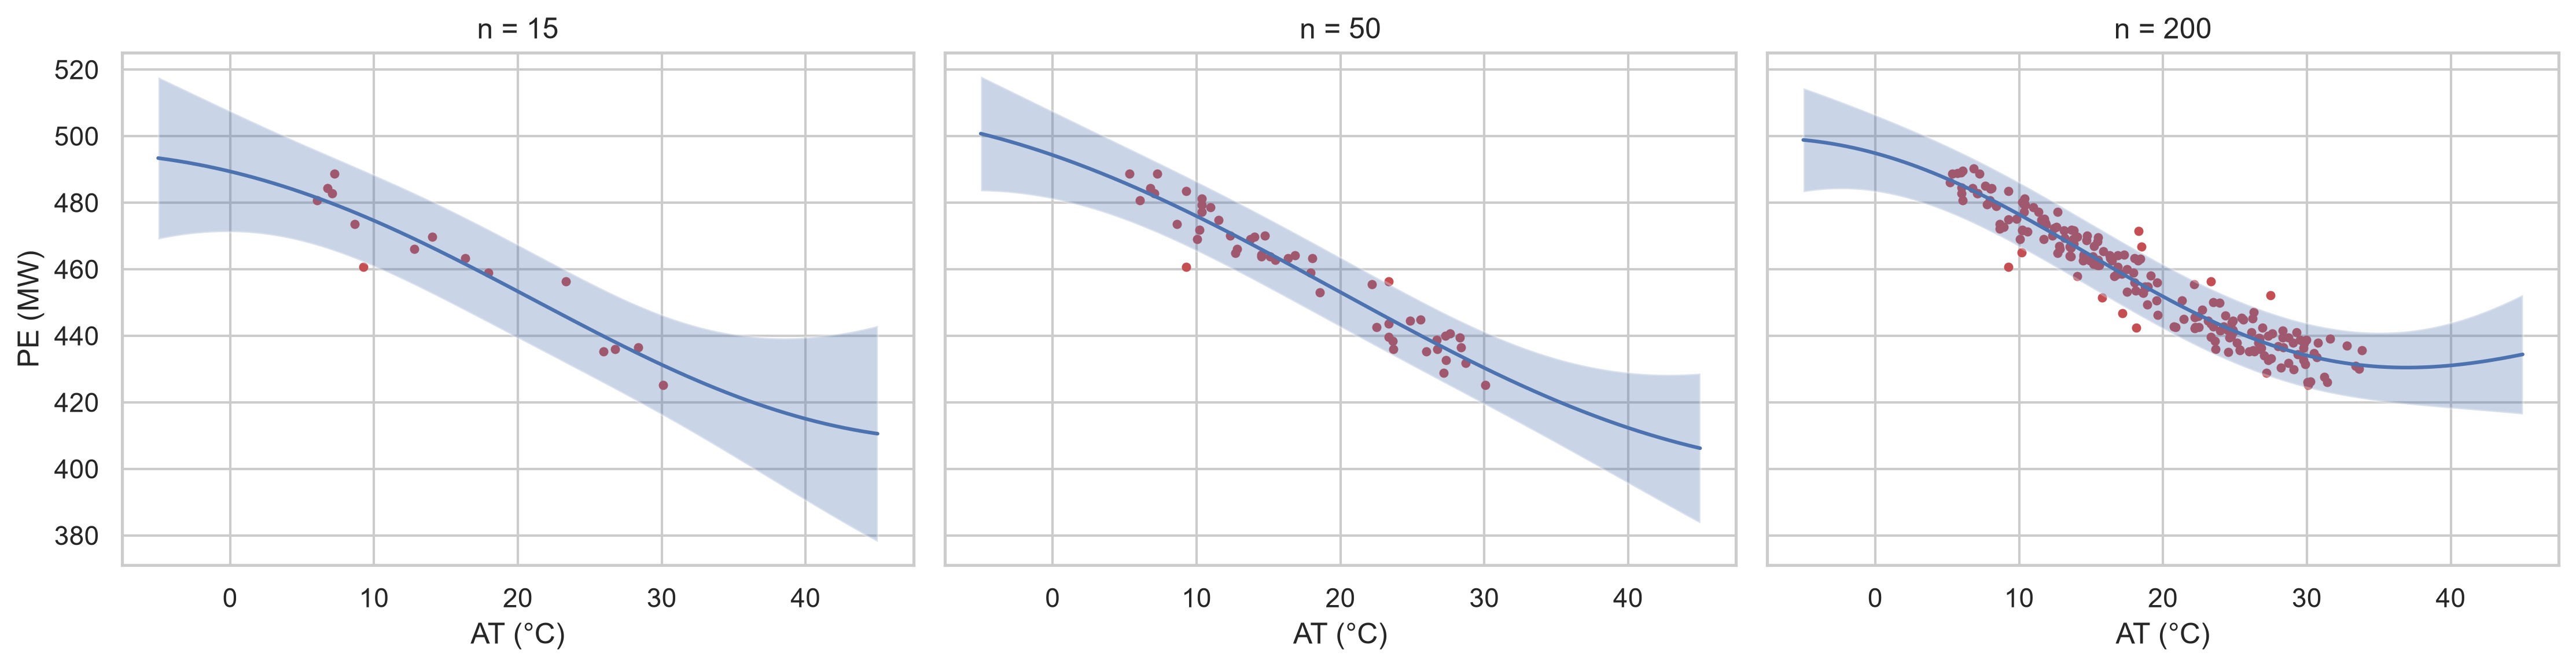
\includegraphics[keepaspectratio]{notebooks/06-model-selection_files/figure-pdf/cell-13-output-1.png}}

With more data the band becomes narrower, but it does not shrink to
zero: because the kernel contains a \texttt{WhiteKernel}, the predicted
standard deviation includes the measurement noise, so the band
approaches the scatter of individual observations (similar to a
prediction interval). The uncertainty about the \emph{trend} itself,
however, decreases. Outside the data range the band still widens; with
more points the trend is better determined, so the widening is less
dramatic. Where there are no data at all, data elsewhere can only reduce
the uncertainty as far as the kernel assumes smoothness.

\end{tcolorbox}

\begin{tcolorbox}[enhanced jigsaw, colframe=quarto-callout-caution-color-frame, toprule=.15mm, rightrule=.15mm, title=\textcolor{quarto-callout-caution-color}{\faFire}\hspace{0.5em}{Solution to Exercise 5}, colbacktitle=quarto-callout-caution-color!10!white, left=2mm, titlerule=0mm, bottomtitle=1mm, toptitle=1mm, opacityback=0, bottomrule=.15mm, breakable, arc=.35mm, opacitybacktitle=0.6, colback=white, coltitle=black, leftrule=.75mm]

\begin{Shaded}
\begin{Highlighting}[]
\ImportTok{from}\NormalTok{ sklearn.linear\_model }\ImportTok{import}\NormalTok{ LassoCV}

\NormalTok{lasso }\OperatorTok{=}\NormalTok{ make\_pipeline(PolynomialFeatures(}\DecValTok{3}\NormalTok{), StandardScaler(),}
\NormalTok{                      LassoCV(cv}\OperatorTok{=}\DecValTok{5}\NormalTok{, random\_state}\OperatorTok{=}\DecValTok{0}\NormalTok{, max\_iter}\OperatorTok{=}\DecValTok{50000}\NormalTok{)).fit(X, y)}
\NormalTok{coefs }\OperatorTok{=}\NormalTok{ lasso[}\OperatorTok{{-}}\DecValTok{1}\NormalTok{].coef\_}
\NormalTok{names }\OperatorTok{=}\NormalTok{ lasso[}\DecValTok{0}\NormalTok{].get\_feature\_names\_out(X.columns)}
\BuiltInTok{print}\NormalTok{(}\SpecialStringTok{f"}\SpecialCharTok{\{}\NormalTok{(coefs }\OperatorTok{!=} \DecValTok{0}\NormalTok{)}\SpecialCharTok{.}\BuiltInTok{sum}\NormalTok{()}\SpecialCharTok{\}}\SpecialStringTok{ of }\SpecialCharTok{\{}\BuiltInTok{len}\NormalTok{(coefs)}\SpecialCharTok{\}}\SpecialStringTok{ features survive"}\NormalTok{)}
\NormalTok{pd.Series(coefs, index}\OperatorTok{=}\NormalTok{names)[coefs }\OperatorTok{!=} \DecValTok{0}\NormalTok{].sort\_values(key}\OperatorTok{=}\BuiltInTok{abs}\NormalTok{, ascending}\OperatorTok{=}\VariableTok{False}\NormalTok{).head(}\DecValTok{10}\NormalTok{).}\BuiltInTok{round}\NormalTok{(}\DecValTok{3}\NormalTok{)}
\end{Highlighting}
\end{Shaded}

\begin{verbatim}
22 of 56 features survive
\end{verbatim}

\begin{verbatim}
frequency chord         -5.804
frequency thickness     -4.006
frequency^2 chord        1.969
frequency angle chord   -1.947
angle                   -1.946
angle chord velocity     1.935
frequency chord^2        1.800
chord                   -1.715
frequency thickness^2    1.547
frequency^2             -1.390
dtype: float64
\end{verbatim}

Lasso keeps only part of the polynomial terms. The surviving terms show
which inputs and interactions matter most; frequency usually dominates,
since the noise spectrum depends strongly on it. Note that with
correlated features Lasso picks one of a group somewhat arbitrarily --
the selection is not a proof of physical relevance.

\end{tcolorbox}

\begin{tcolorbox}[enhanced jigsaw, colframe=quarto-callout-caution-color-frame, toprule=.15mm, rightrule=.15mm, title=\textcolor{quarto-callout-caution-color}{\faFire}\hspace{0.5em}{Solution to Exercise 6}, colbacktitle=quarto-callout-caution-color!10!white, left=2mm, titlerule=0mm, bottomtitle=1mm, toptitle=1mm, opacityback=0, bottomrule=.15mm, breakable, arc=.35mm, opacitybacktitle=0.6, colback=white, coltitle=black, leftrule=.75mm]

Change \texttt{X\_runs} to, e.g.,
\texttt{{[}{[}100.0{]},\ {[}130.0{]},\ {[}250.0{]}{]}} and rerun the
loop. Usually the algorithm still finds the region of the optimum,
because the large uncertainty in unexplored regions makes EI large
there. With an unlucky start and a misleading local maximum (the sine
term), it may need more iterations. A regular grid of 8 runs over
100--250 °C has a spacing of about 21 °C; the best grid point can easily
be several percent below the true optimum, and the grid cannot refine
itself. Bayesian optimisation pays off when each run is expensive and
runs can be performed one after another.

\end{tcolorbox}

\part{Part C -- Machine Learning}

\chapter{Classification}\label{classification}

Many engineering decisions are categorical: a part is OK or not OK, a
machine will fail within the next shift or not, a fault belongs to type
A, B or C. Predicting such a category from measured data is called
\textbf{classification}. It is the core of automated quality inspection,
predictive maintenance and fault diagnosis.

Classification raises questions that regression does not. How do we
measure the quality of a classifier when failures are rare? What is
worse -- a false alarm or a missed failure? And how do we choose the
decision threshold that turns a predicted probability into an action?
This chapter introduces three basic classifiers and, just as
importantly, the metrics to evaluate them honestly.

\textbf{Scenario: should we install the failure alarm?}

A milling line runs 10,000 operations per period. Every machine failure
that is not anticipated costs about 10,000 € (scrap, repair, downtime).
A vendor offers to install a failure alarm: when it fires, the machine
is stopped and inspected, which costs about 500 € -- whether or not a
failure was imminent. Today there is no alarm at all, so every failure
is unplanned. The plant manager wants a clear answer.

\textbf{Your decision:} Install an alarm -- and if so, based on which
model?

\textbf{Learning goals.} After this chapter you can

\begin{itemize}
\tightlist
\item
  explain how logistic regression, k-nearest neighbours and decision
  trees classify,
\item
  evaluate classifiers with confusion matrix, precision, recall, F1, ROC
  and precision--recall curves,
\item
  handle strongly imbalanced classes with class weights, suitable
  metrics and threshold choice,
\item
  choose a decision threshold based on the costs of errors,
\item
  recognise and avoid data leakage.
\end{itemize}

\textbf{Datasets in this chapter}

\begin{itemize}
\tightlist
\item
  \href{https://archive.ics.uci.edu/dataset/601/ai4i+2020+predictive+maintenance+dataset}{AI4I
  2020 Predictive Maintenance (UCI)}
\end{itemize}

\section{Three ways to classify}\label{three-ways-to-classify}

In classification, the response \(y\) takes one of \(K\) classes; in the
\textbf{binary} case \(y \in \{0, 1\}\) (e.g.~1 = failure). Most
classifiers estimate the probability \(P(y = 1 \mid x)\) and predict
class 1 if this probability exceeds a \textbf{threshold}, by default
0.5.

\subsection{Logistic regression}\label{logistic-regression}

\begin{tcolorbox}[enhanced jigsaw, colframe=quarto-callout-note-color-frame, toprule=.15mm, rightrule=.15mm, title=\textcolor{quarto-callout-note-color}{\faInfo}\hspace{0.5em}{Definition: Logistic regression}, colbacktitle=quarto-callout-note-color!10!white, left=2mm, titlerule=0mm, bottomtitle=1mm, toptitle=1mm, opacityback=0, bottomrule=.15mm, breakable, arc=.35mm, opacitybacktitle=0.6, colback=white, coltitle=black, leftrule=.75mm]

The probability of class 1 is modelled as
\[P(y = 1 \mid x) = \sigma(\beta_0 + \beta^\top x), \qquad \sigma(z) = \frac{1}{1 + e^{-z}}.\]
Equivalently, the \textbf{log-odds} are linear in the inputs:
\(\ln\frac{P(y=1\mid x)}{1 - P(y=1\mid x)} = \beta_0 + \beta^\top x\).
The parameters are estimated by maximum likelihood.

\end{tcolorbox}

Logistic regression is the classification counterpart of linear
regression: simple, fast, interpretable. A coefficient \(\beta_j\) means
that one unit more of \(x_j\) multiplies the odds of failure by
\(e^{\beta_j}\) (the \textbf{odds ratio}). Its decision boundary -- the
set of \(x\) where the probability equals the threshold -- is a straight
line (a hyperplane). Nonlinear boundaries require engineered features
such as products or squares.

\subsection{k-nearest neighbours (kNN)}\label{k-nearest-neighbours-knn}

kNN stores the training data and classifies a new point by majority vote
of its \(k\) nearest training points. It makes no assumption about the
shape of the boundary, but it depends entirely on the \textbf{distance
measure} -- inputs must be standardised, otherwise the input with the
largest numerical range dominates. Small \(k\) gives ragged boundaries
(high variance), large \(k\) smooth ones (high bias).

\subsection{Decision trees}\label{decision-trees}

A decision tree splits the input space step by step with simple rules
such as ``torque \textgreater{} 55 Nm''. At each node, the split is
chosen that makes the resulting groups as \textbf{pure} as possible,
measured e.g.~by the Gini impurity \(G = 1 - \sum_k p_k^2\), where
\(p_k\) is the share of class \(k\) in the node. Trees are easy to
explain to colleagues and can capture interactions and thresholds, but a
single deep tree overfits strongly; its depth must be limited. Chapter 8
shows how combining many trees fixes this.

\begin{figure}[H]

\centering{

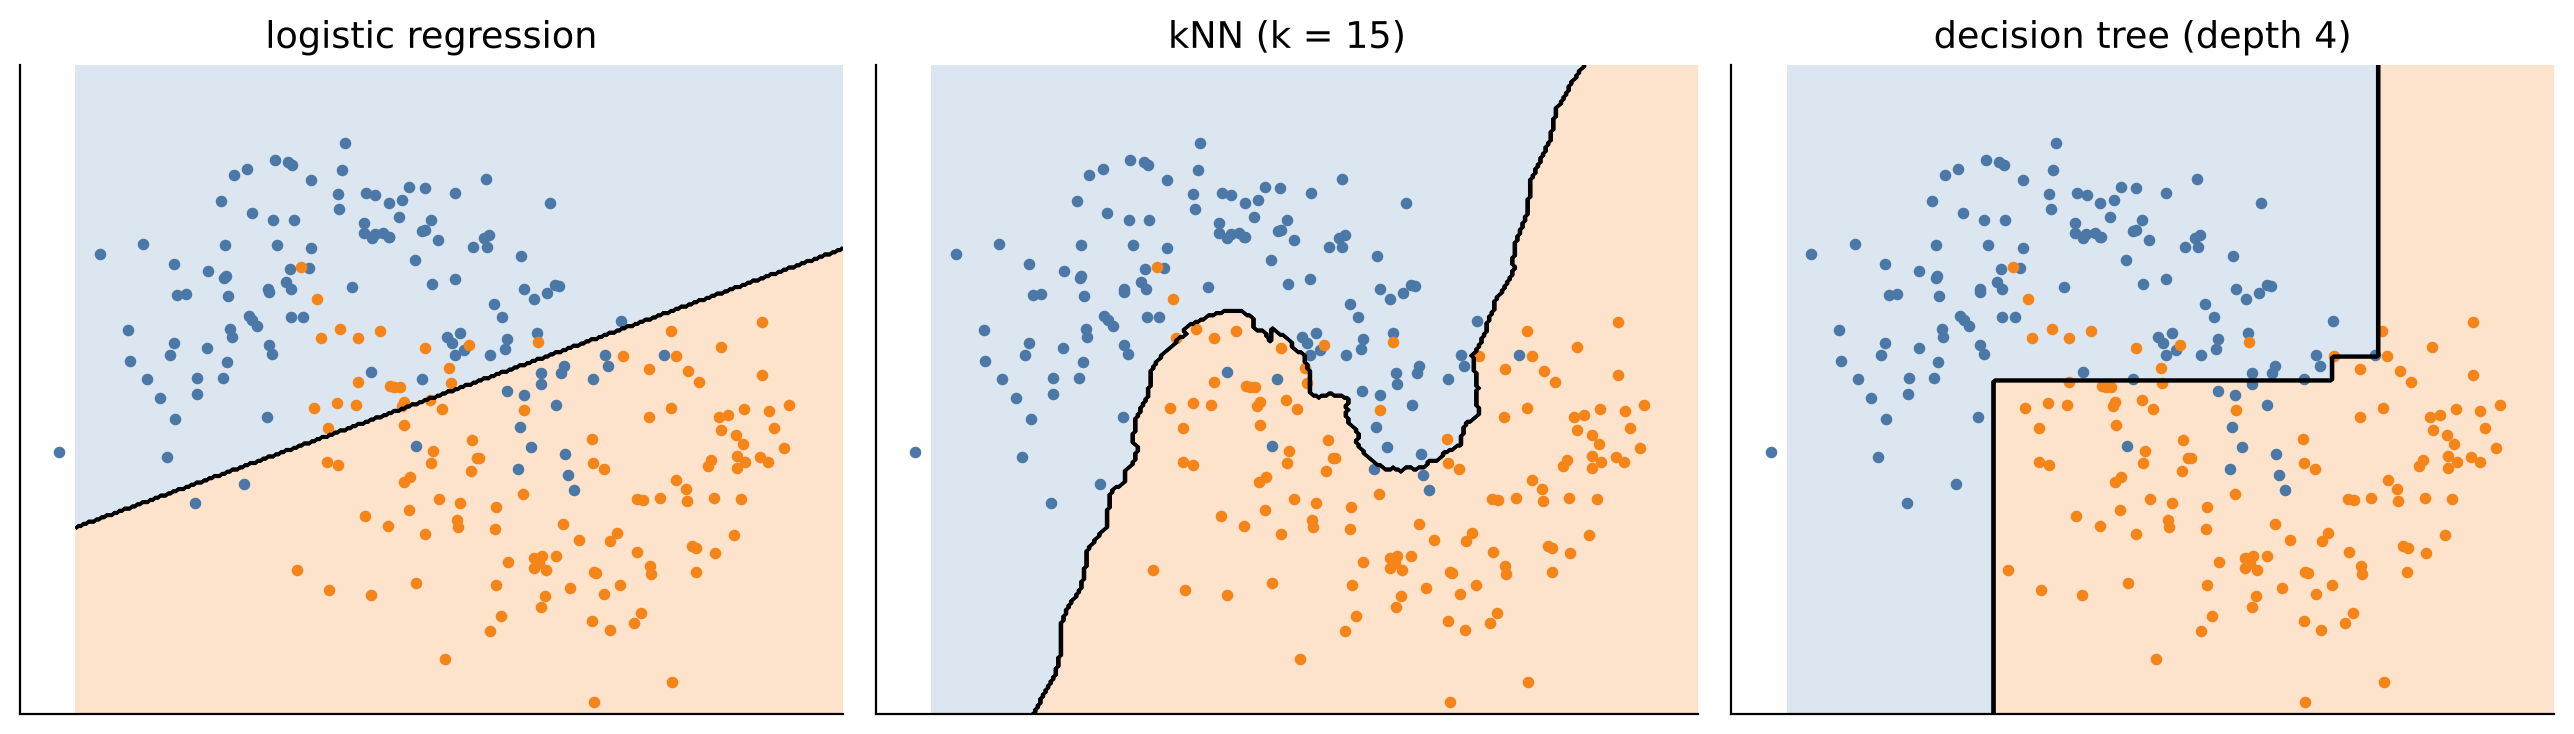
\includegraphics[width=1\linewidth,height=\textheight,keepaspectratio]{notebooks/images/decision-boundaries.png}

}

\caption{\label{fig-boundaries}Decision boundaries of the three
classifiers on a two-dimensional toy problem. Logistic regression draws
a straight line, kNN follows the local structure of the data, and a
decision tree uses axis-parallel steps.}

\end{figure}%

\section{Evaluating classifiers}\label{evaluating-classifiers}

\begin{tcolorbox}[enhanced jigsaw, colframe=quarto-callout-note-color-frame, toprule=.15mm, rightrule=.15mm, title=\textcolor{quarto-callout-note-color}{\faInfo}\hspace{0.5em}{Definition: Confusion matrix and derived metrics}, colbacktitle=quarto-callout-note-color!10!white, left=2mm, titlerule=0mm, bottomtitle=1mm, toptitle=1mm, opacityback=0, bottomrule=.15mm, breakable, arc=.35mm, opacitybacktitle=0.6, colback=white, coltitle=black, leftrule=.75mm]

\begin{longtable}[]{@{}
  >{\raggedright\arraybackslash}p{(\linewidth - 4\tabcolsep) * \real{0.3333}}
  >{\raggedright\arraybackslash}p{(\linewidth - 4\tabcolsep) * \real{0.3333}}
  >{\raggedright\arraybackslash}p{(\linewidth - 4\tabcolsep) * \real{0.3333}}@{}}
\toprule\noalign{}
\begin{minipage}[b]{\linewidth}\raggedright
\end{minipage} & \begin{minipage}[b]{\linewidth}\raggedright
predicted OK (0)
\end{minipage} & \begin{minipage}[b]{\linewidth}\raggedright
predicted failure (1)
\end{minipage} \\
\midrule\noalign{}
\endhead
\bottomrule\noalign{}
\endlastfoot
\textbf{actual OK (0)} & true negative (TN) & false positive (FP) --
false alarm \\
\textbf{actual failure (1)} & false negative (FN) -- missed failure &
true positive (TP) \\
\end{longtable}

\begin{itemize}
\tightlist
\item
  \textbf{Accuracy} = (TP + TN) / all
\item
  \textbf{Precision} = TP / (TP + FP): how many alarms are real?
\item
  \textbf{Recall} (sensitivity, detection rate) = TP / (TP + FN): how
  many failures are detected?
\item
  \textbf{F1 score} = harmonic mean of precision and recall
\item
  \textbf{Balanced accuracy} = mean of the recall of both classes
\end{itemize}

\end{tcolorbox}

\begin{tcolorbox}[enhanced jigsaw, colframe=quarto-callout-warning-color-frame, toprule=.15mm, rightrule=.15mm, title=\textcolor{quarto-callout-warning-color}{\faExclamationTriangle}\hspace{0.5em}{Pitfall: accuracy on imbalanced data}, colbacktitle=quarto-callout-warning-color!10!white, left=2mm, titlerule=0mm, bottomtitle=1mm, toptitle=1mm, opacityback=0, bottomrule=.15mm, breakable, arc=.35mm, opacitybacktitle=0.6, colback=white, coltitle=black, leftrule=.75mm]

If 3 \% of the records are failures, a ``model'' that always predicts
``OK'' reaches 97 \% accuracy -- and detects nothing. With rare events,
accuracy is almost meaningless. Use precision, recall, F1 or balanced
accuracy, and always look at the confusion matrix.

\end{tcolorbox}

Precision is nothing but \(P(\text{failure} \mid \text{alarm})\) --
Bayes' theorem from Chapter 3. When failures are rare, even a detector
with high recall and a low false alarm rate can have a low precision.

\subsection{Thresholds, ROC and precision--recall
curves}\label{thresholds-roc-and-precisionrecall-curves}

Lowering the threshold produces more alarms: recall increases, precision
usually decreases. Instead of judging a single threshold, we can look at
all thresholds at once:

\begin{itemize}
\tightlist
\item
  The \textbf{ROC curve} plots the true positive rate (recall) against
  the false positive rate FP/(FP + TN). The area under the curve
  (\textbf{ROC AUC}) is the probability that a randomly chosen failure
  gets a higher score than a randomly chosen OK record; 0.5 = random
  guessing, 1 = perfect ranking.
\item
  The \textbf{precision--recall curve} plots precision against recall.
  For rare events it is more informative than ROC, because the false
  positive \emph{rate} stays small even when the false alarms far
  outnumber the true alarms.
\end{itemize}

\begin{tcolorbox}[enhanced jigsaw, colframe=quarto-callout-tip-color-frame, toprule=.15mm, rightrule=.15mm, title=\textcolor{quarto-callout-tip-color}{\faLightbulb}\hspace{0.5em}{Engineering practice: choose the threshold by costs}, colbacktitle=quarto-callout-tip-color!10!white, left=2mm, titlerule=0mm, bottomtitle=1mm, toptitle=1mm, opacityback=0, bottomrule=.15mm, breakable, arc=.35mm, opacitybacktitle=0.6, colback=white, coltitle=black, leftrule=.75mm]

The threshold 0.5 is arbitrary. If a missed failure costs \(c_{FN}\) and
a false alarm \(c_{FP}\), choose the threshold that minimises the total
cost \(c_{FN} \cdot \text{FN} + c_{FP} \cdot \text{FP}\) -- on
validation data, not on the test data. For well-calibrated
probabilities, the optimal threshold is \(c_{FP}/(c_{FP} + c_{FN})\): if
a miss is 20 times as expensive as a false alarm, alarm already at a
failure probability of about 5 \%.

\end{tcolorbox}

\subsection{Strategies for imbalanced
classes}\label{strategies-for-imbalanced-classes}

\begin{itemize}
\tightlist
\item
  \textbf{Stratified splitting:} keep the class proportions equal in
  training and test data (\texttt{stratify=y}).
\item
  \textbf{Class weights:} weight errors on the rare class more strongly
  during training (\texttt{class\_weight="balanced"}).
\item
  \textbf{Resampling:} undersample the majority class or oversample the
  minority class (only in the training data!).
\item
  \textbf{Threshold adjustment} as described above -- often the simplest
  and most effective measure.
\end{itemize}

\begin{Shaded}
\begin{Highlighting}[]
\CommentTok{\# Setup: works locally and in Google Colab}
\ImportTok{import}\NormalTok{ importlib.util, subprocess, sys}
\ControlFlowTok{for}\NormalTok{ pkg }\KeywordTok{in}\NormalTok{ [}\StringTok{"ucimlrepo"}\NormalTok{]:}
    \ControlFlowTok{if}\NormalTok{ importlib.util.find\_spec(pkg) }\KeywordTok{is} \VariableTok{None}\NormalTok{:}
\NormalTok{        subprocess.run([sys.executable, }\StringTok{"{-}m"}\NormalTok{, }\StringTok{"pip"}\NormalTok{, }\StringTok{"install"}\NormalTok{, }\StringTok{"{-}q"}\NormalTok{, pkg], check}\OperatorTok{=}\VariableTok{True}\NormalTok{)}

\ImportTok{import}\NormalTok{ numpy }\ImportTok{as}\NormalTok{ np}
\ImportTok{import}\NormalTok{ pandas }\ImportTok{as}\NormalTok{ pd}
\ImportTok{import}\NormalTok{ matplotlib.pyplot }\ImportTok{as}\NormalTok{ plt}
\ImportTok{import}\NormalTok{ seaborn }\ImportTok{as}\NormalTok{ sns}

\NormalTok{sns.set\_theme(style}\OperatorTok{=}\StringTok{"whitegrid"}\NormalTok{)}
\end{Highlighting}
\end{Shaded}

\section{Live coding: predictive
maintenance}\label{live-coding-predictive-maintenance}

The AI4I 2020 dataset is a synthetic dataset that reflects a real
milling process. Each of the 10,000 records contains the product quality
variant (L/M/H), air and process temperature, rotational speed, torque
and tool wear, and the label \texttt{Machine\ failure}. The failures are
generated by five documented mechanisms: tool wear failure (TWF), heat
dissipation failure (HDF), power failure (PWF), overstrain failure (OSF)
and random failures (RNF). Because the mechanisms are known, the dataset
is ideal to check whether a model has learned something physically
sensible.

\begin{Shaded}
\begin{Highlighting}[]
\ImportTok{from}\NormalTok{ ucimlrepo }\ImportTok{import}\NormalTok{ fetch\_ucirepo}

\NormalTok{ai4i }\OperatorTok{=}\NormalTok{ fetch\_ucirepo(}\BuiltInTok{id}\OperatorTok{=}\DecValTok{601}\NormalTok{).data.original}

\CommentTok{\# Column names differ between versions of the dataset (with or without units in brackets,}
\CommentTok{\# blanks or underscores). We map them to one canonical spelling with units.}
\ImportTok{import}\NormalTok{ re}
\NormalTok{canonical }\OperatorTok{=}\NormalTok{ \{}\StringTok{"air temperature"}\NormalTok{: }\StringTok{"Air temperature [K]"}\NormalTok{, }\StringTok{"process temperature"}\NormalTok{: }\StringTok{"Process temperature [K]"}\NormalTok{,}
             \StringTok{"rotational speed"}\NormalTok{: }\StringTok{"Rotational speed [rpm]"}\NormalTok{, }\StringTok{"torque"}\NormalTok{: }\StringTok{"Torque [Nm]"}\NormalTok{,}
             \StringTok{"tool wear"}\NormalTok{: }\StringTok{"Tool wear [min]"}\NormalTok{, }\StringTok{"machine failure"}\NormalTok{: }\StringTok{"Machine failure"}\NormalTok{, }\StringTok{"type"}\NormalTok{: }\StringTok{"Type"}\NormalTok{\}}
\KeywordTok{def}\NormalTok{ standardise(col):}
\NormalTok{    base }\OperatorTok{=}\NormalTok{ re.sub(}\VerbatimStringTok{r"[\_\textbackslash{}s]+"}\NormalTok{, }\StringTok{" "}\NormalTok{, }\BuiltInTok{str}\NormalTok{(col).split(}\StringTok{"["}\NormalTok{)[}\DecValTok{0}\NormalTok{]).strip().lower()}
    \ControlFlowTok{return}\NormalTok{ canonical.get(base, col)}
\NormalTok{ai4i }\OperatorTok{=}\NormalTok{ ai4i.rename(columns}\OperatorTok{=}\NormalTok{standardise)}
\BuiltInTok{print}\NormalTok{(}\StringTok{"Columns:"}\NormalTok{, ai4i.columns.tolist())}

\NormalTok{features }\OperatorTok{=}\NormalTok{ [}\StringTok{"Type"}\NormalTok{, }\StringTok{"Air temperature [K]"}\NormalTok{, }\StringTok{"Process temperature [K]"}\NormalTok{,}
            \StringTok{"Rotational speed [rpm]"}\NormalTok{, }\StringTok{"Torque [Nm]"}\NormalTok{, }\StringTok{"Tool wear [min]"}\NormalTok{]}
\NormalTok{X }\OperatorTok{=}\NormalTok{ pd.get\_dummies(ai4i[features], columns}\OperatorTok{=}\NormalTok{[}\StringTok{"Type"}\NormalTok{], drop\_first}\OperatorTok{=}\VariableTok{True}\NormalTok{)}
\NormalTok{y }\OperatorTok{=}\NormalTok{ ai4i[}\StringTok{"Machine failure"}\NormalTok{]}
\BuiltInTok{print}\NormalTok{(}\SpecialStringTok{f"Failure rate: }\SpecialCharTok{\{}\NormalTok{y}\SpecialCharTok{.}\NormalTok{mean()}\SpecialCharTok{:.1\%\}}\SpecialStringTok{"}\NormalTok{)}
\CommentTok{\# }\AlertTok{NOTE}\CommentTok{: the columns TWF, HDF, PWF, OSF, RNF describe the failure mode.}
\CommentTok{\# Using them as features would be data leakage!}
\end{Highlighting}
\end{Shaded}

\begin{verbatim}
Columns: ['UID', 'Product ID', 'Type', 'Air temperature [K]', 'Process temperature [K]', 'Rotational speed [rpm]', 'Torque [Nm]', 'Tool wear [min]', 'Machine failure', 'TWF', 'HDF', 'PWF', 'OSF', 'RNF']
Failure rate: 3.4%
\end{verbatim}

\begin{Shaded}
\begin{Highlighting}[]
\NormalTok{sns.scatterplot(data}\OperatorTok{=}\NormalTok{ai4i.sample(}\DecValTok{3000}\NormalTok{, random\_state}\OperatorTok{=}\DecValTok{0}\NormalTok{), x}\OperatorTok{=}\StringTok{"Rotational speed [rpm]"}\NormalTok{, y}\OperatorTok{=}\StringTok{"Torque [Nm]"}\NormalTok{,}
\NormalTok{                hue}\OperatorTok{=}\StringTok{"Machine failure"}\NormalTok{, s}\OperatorTok{=}\DecValTok{10}\NormalTok{, alpha}\OperatorTok{=}\FloatTok{0.6}\NormalTok{, palette}\OperatorTok{=}\NormalTok{[}\StringTok{"lightgray"}\NormalTok{, }\StringTok{"C3"}\NormalTok{])}
\NormalTok{plt.show()}
\end{Highlighting}
\end{Shaded}

\pandocbounded{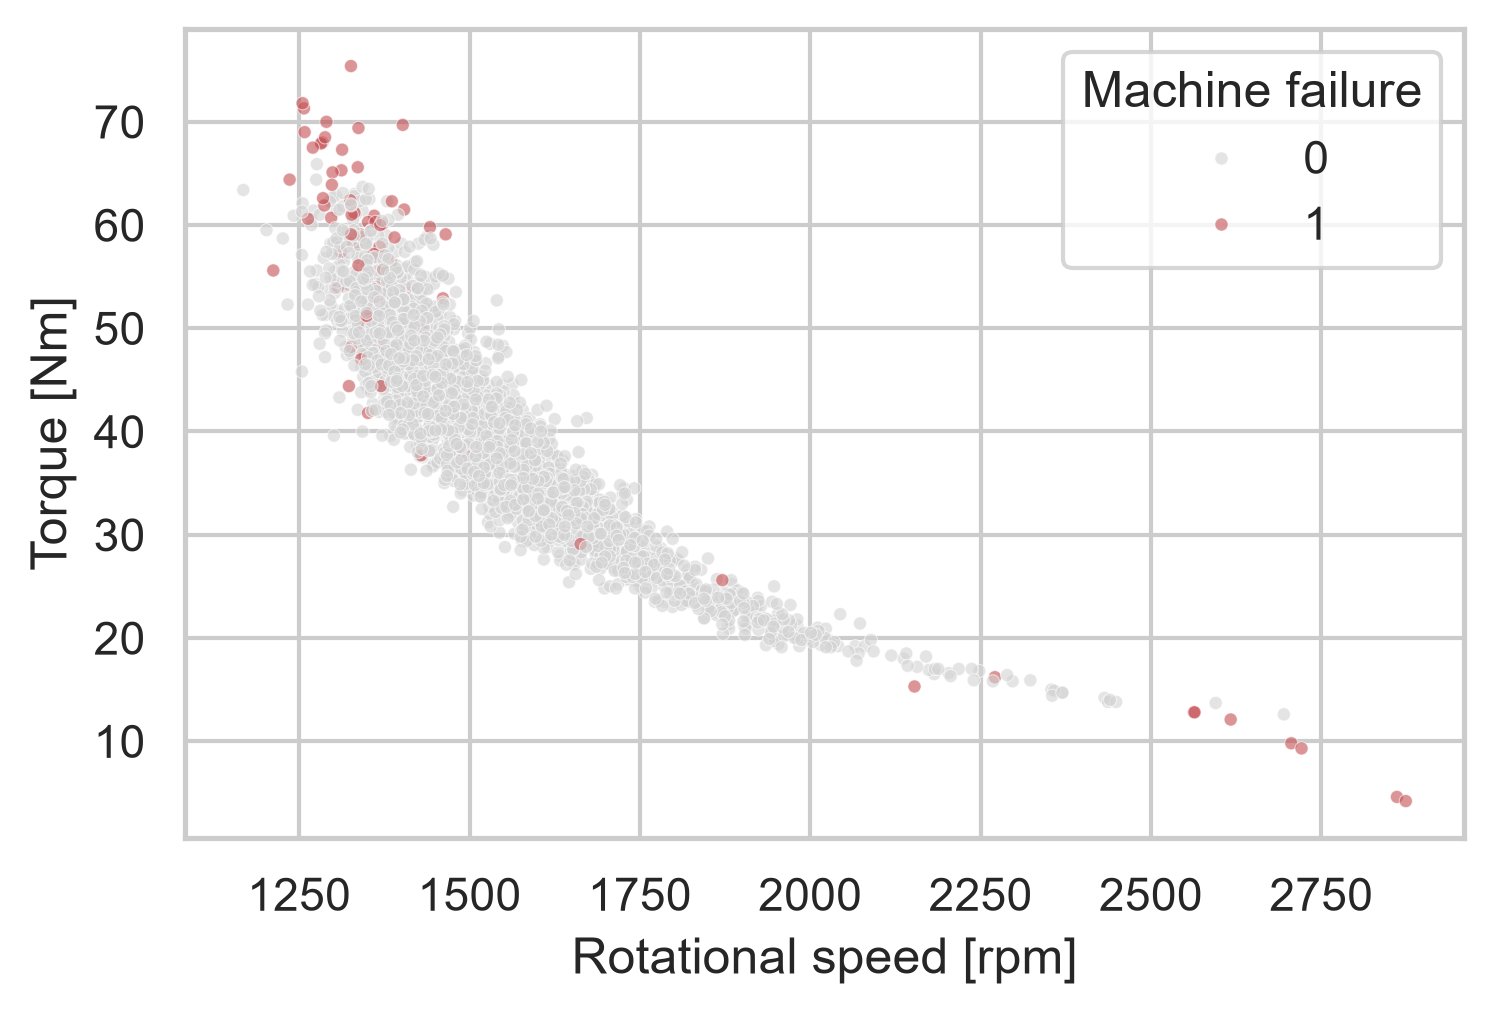
\includegraphics[keepaspectratio]{notebooks/07-classification_files/figure-pdf/cell-4-output-1.png}}

The failures are not spread randomly: they concentrate at very high
torque with low speed and at very low torque with high speed -- regions
of high and low mechanical power. A linear boundary in this plane cannot
separate them; this matters for the choice of model.

\begin{Shaded}
\begin{Highlighting}[]
\ImportTok{from}\NormalTok{ sklearn.model\_selection }\ImportTok{import}\NormalTok{ train\_test\_split}
\ImportTok{from}\NormalTok{ sklearn.pipeline }\ImportTok{import}\NormalTok{ make\_pipeline}
\ImportTok{from}\NormalTok{ sklearn.preprocessing }\ImportTok{import}\NormalTok{ StandardScaler}
\ImportTok{from}\NormalTok{ sklearn.linear\_model }\ImportTok{import}\NormalTok{ LogisticRegression}
\ImportTok{from}\NormalTok{ sklearn.neighbors }\ImportTok{import}\NormalTok{ KNeighborsClassifier}
\ImportTok{from}\NormalTok{ sklearn.tree }\ImportTok{import}\NormalTok{ DecisionTreeClassifier}
\ImportTok{from}\NormalTok{ sklearn.metrics }\ImportTok{import}\NormalTok{ classification\_report}

\NormalTok{X\_train, X\_test, y\_train, y\_test }\OperatorTok{=}\NormalTok{ train\_test\_split(}
\NormalTok{    X, y, test\_size}\OperatorTok{=}\FloatTok{0.25}\NormalTok{, stratify}\OperatorTok{=}\NormalTok{y, random\_state}\OperatorTok{=}\DecValTok{0}\NormalTok{)}

\NormalTok{models }\OperatorTok{=}\NormalTok{ \{}
    \StringTok{"logistic regression"}\NormalTok{: make\_pipeline(StandardScaler(), LogisticRegression(class\_weight}\OperatorTok{=}\StringTok{"balanced"}\NormalTok{, max\_iter}\OperatorTok{=}\DecValTok{1000}\NormalTok{)),}
    \StringTok{"kNN (k=5)"}\NormalTok{: make\_pipeline(StandardScaler(), KNeighborsClassifier(}\DecValTok{5}\NormalTok{)),}
    \StringTok{"decision tree"}\NormalTok{: DecisionTreeClassifier(max\_depth}\OperatorTok{=}\DecValTok{5}\NormalTok{, class\_weight}\OperatorTok{=}\StringTok{"balanced"}\NormalTok{, random\_state}\OperatorTok{=}\DecValTok{0}\NormalTok{),}
\NormalTok{\}}
\ControlFlowTok{for}\NormalTok{ name, m }\KeywordTok{in}\NormalTok{ models.items():}
\NormalTok{    m.fit(X\_train, y\_train)}
    \BuiltInTok{print}\NormalTok{(}\SpecialStringTok{f"{-}{-}{-} }\SpecialCharTok{\{}\NormalTok{name}\SpecialCharTok{\}}\SpecialStringTok{"}\NormalTok{)}
    \BuiltInTok{print}\NormalTok{(classification\_report(y\_test, m.predict(X\_test), digits}\OperatorTok{=}\DecValTok{3}\NormalTok{))}
\end{Highlighting}
\end{Shaded}

\begin{verbatim}
--- logistic regression
              precision    recall  f1-score   support

           0      0.990     0.827     0.901      2415
           1      0.135     0.765     0.229        85

    accuracy                          0.825      2500
   macro avg      0.562     0.796     0.565      2500
weighted avg      0.961     0.825     0.878      2500

--- kNN (k=5)
              precision    recall  f1-score   support

           0      0.977     0.996     0.986      2415
           1      0.737     0.329     0.455        85

    accuracy                          0.973      2500
   macro avg      0.857     0.663     0.721      2500
weighted avg      0.969     0.973     0.968      2500

--- decision tree
              precision    recall  f1-score   support

           0      0.994     0.935     0.964      2415
           1      0.311     0.835     0.454        85

    accuracy                          0.932      2500
   macro avg      0.653     0.885     0.709      2500
weighted avg      0.971     0.932     0.946      2500
\end{verbatim}

\textbf{Discussion.} Read the reports row by row: the line for class 1
(failure) is the interesting one. Typically, logistic regression with
class weights detects many failures (high recall) but raises many false
alarms (low precision), because its linear boundary cannot isolate the
failure regions. kNN without class weights is conservative: few false
alarms, but many missed failures. The decision tree can represent the
thresholds in torque, speed and tool wear that generate the failures and
usually achieves the best balance. The accuracy row is high for all
models -- and says little.

\begin{Shaded}
\begin{Highlighting}[]
\ImportTok{from}\NormalTok{ sklearn.metrics }\ImportTok{import}\NormalTok{ ConfusionMatrixDisplay, PrecisionRecallDisplay, RocCurveDisplay}

\NormalTok{fig, axes }\OperatorTok{=}\NormalTok{ plt.subplots(}\DecValTok{1}\NormalTok{, }\DecValTok{3}\NormalTok{, figsize}\OperatorTok{=}\NormalTok{(}\DecValTok{16}\NormalTok{, }\FloatTok{4.5}\NormalTok{))}
\NormalTok{ConfusionMatrixDisplay.from\_estimator(models[}\StringTok{"decision tree"}\NormalTok{], X\_test, y\_test, ax}\OperatorTok{=}\NormalTok{axes[}\DecValTok{0}\NormalTok{], colorbar}\OperatorTok{=}\VariableTok{False}\NormalTok{)}
\NormalTok{axes[}\DecValTok{0}\NormalTok{].set\_title(}\StringTok{"Decision tree"}\NormalTok{)}
\ControlFlowTok{for}\NormalTok{ name, m }\KeywordTok{in}\NormalTok{ models.items():}
\NormalTok{    RocCurveDisplay.from\_estimator(m, X\_test, y\_test, ax}\OperatorTok{=}\NormalTok{axes[}\DecValTok{1}\NormalTok{], name}\OperatorTok{=}\NormalTok{name)}
\NormalTok{    PrecisionRecallDisplay.from\_estimator(m, X\_test, y\_test, ax}\OperatorTok{=}\NormalTok{axes[}\DecValTok{2}\NormalTok{], name}\OperatorTok{=}\NormalTok{name)}
\NormalTok{axes[}\DecValTok{1}\NormalTok{].set\_title(}\StringTok{"ROC curves"}\NormalTok{)}\OperatorTok{;}\NormalTok{ axes[}\DecValTok{2}\NormalTok{].set\_title(}\StringTok{"Precision–recall curves"}\NormalTok{)}
\NormalTok{plt.tight\_layout()}\OperatorTok{;}\NormalTok{ plt.show()}
\end{Highlighting}
\end{Shaded}

\pandocbounded{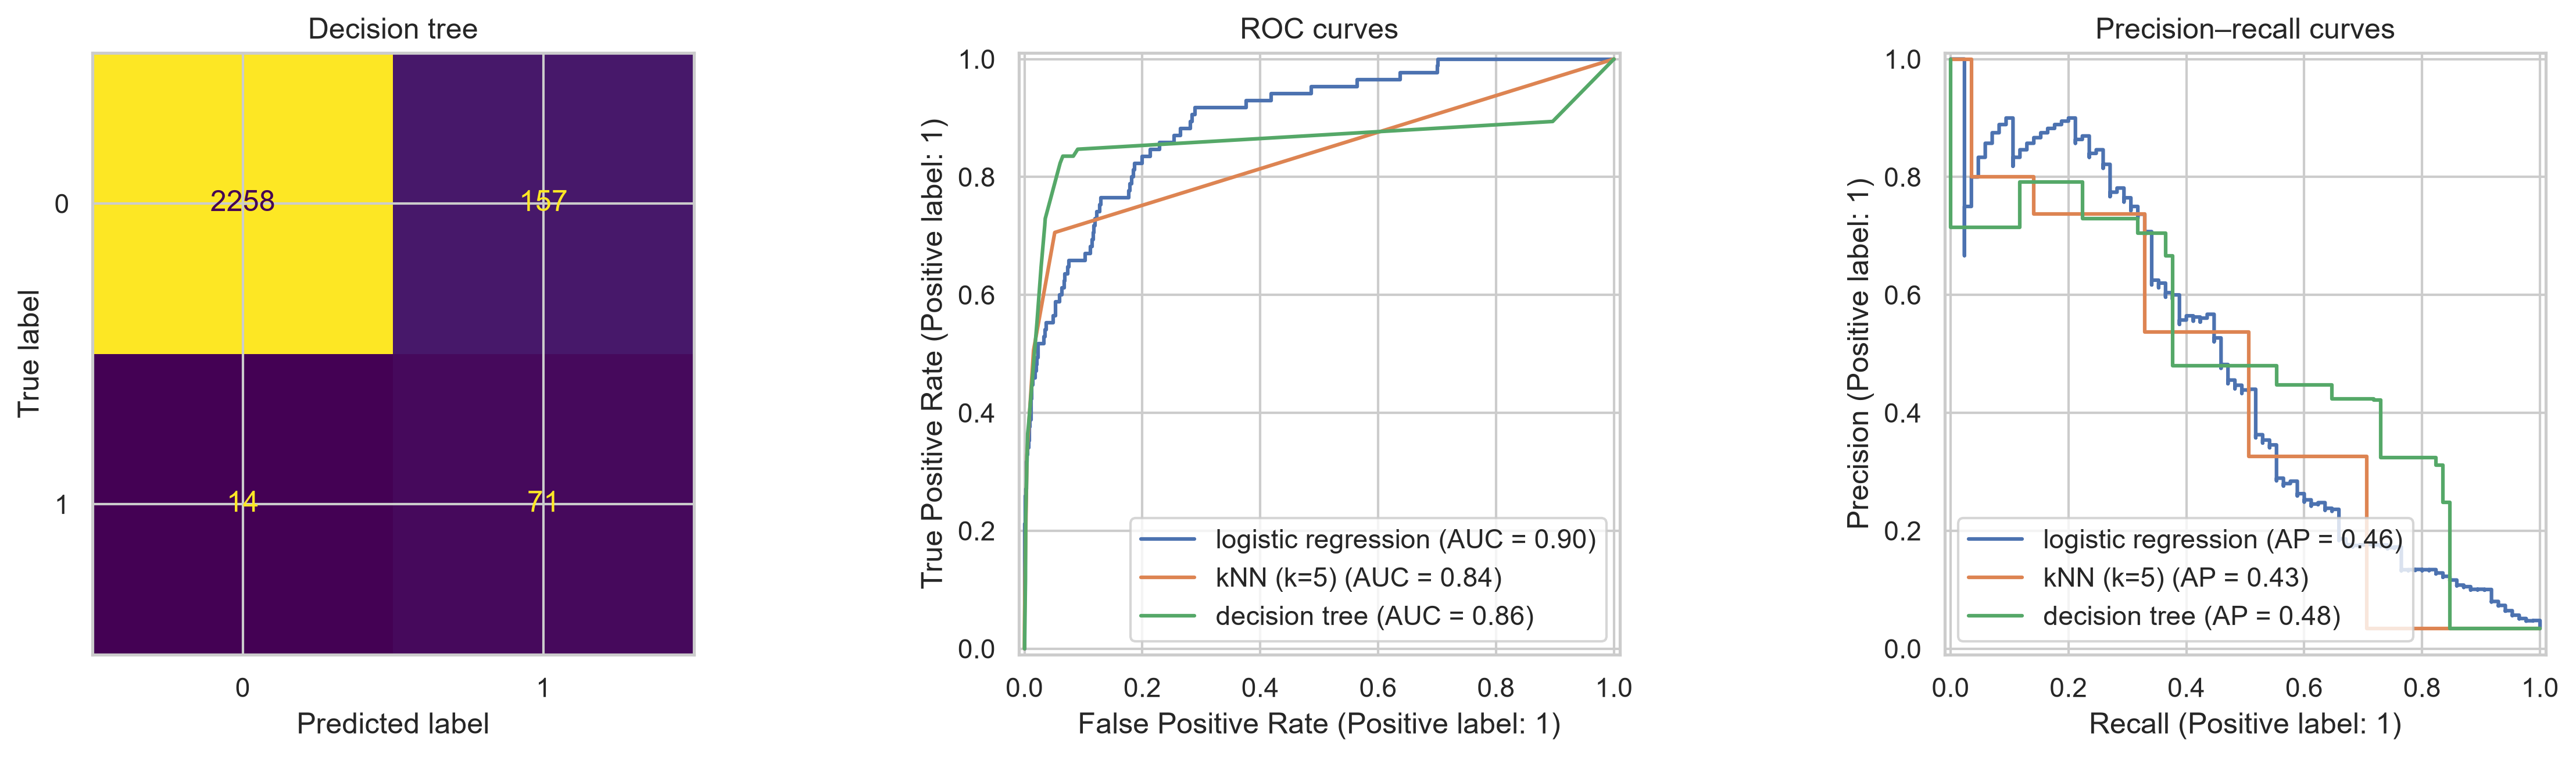
\includegraphics[keepaspectratio]{notebooks/07-classification_files/figure-pdf/cell-6-output-1.png}}

\textbf{Discussion.} The ROC curves may look reassuringly good for all
models, while the precision--recall curves reveal clear differences --
the typical picture for rare events. The precision--recall curve
directly shows the trade-off an engineer faces: ``If I want to catch 80
\% of the failures, how many of my alarms will be false?''

\section{Back to the decision}\label{back-to-the-decision-6}

We compare the total cost per test period for the status quo (every
failure is a missed failure) and for each model at its default
threshold. A missed failure costs 10,000 €, a false alarm 500 €.
Detected failures are assumed to be prevented and to cost only the
inspection.

\begin{Shaded}
\begin{Highlighting}[]
\ImportTok{from}\NormalTok{ sklearn.metrics }\ImportTok{import}\NormalTok{ confusion\_matrix}

\NormalTok{c\_fn, c\_fp }\OperatorTok{=} \DecValTok{10\_000}\NormalTok{, }\DecValTok{500}
\NormalTok{status\_quo }\OperatorTok{=}\NormalTok{ c\_fn }\OperatorTok{*} \BuiltInTok{int}\NormalTok{(y\_test.}\BuiltInTok{sum}\NormalTok{())}
\NormalTok{costs }\OperatorTok{=}\NormalTok{ \{\}}
\ControlFlowTok{for}\NormalTok{ name, m }\KeywordTok{in}\NormalTok{ models.items():}
\NormalTok{    tn, fp, fn, tp }\OperatorTok{=}\NormalTok{ confusion\_matrix(y\_test, m.predict(X\_test)).ravel()}
\NormalTok{    costs[name] }\OperatorTok{=}\NormalTok{ c\_fn }\OperatorTok{*}\NormalTok{ fn }\OperatorTok{+}\NormalTok{ c\_fp }\OperatorTok{*}\NormalTok{ (fp }\OperatorTok{+}\NormalTok{ tp)          }\CommentTok{\# every alarm triggers an inspection}
\BuiltInTok{print}\NormalTok{(}\SpecialStringTok{f"}\SpecialCharTok{\{}\StringTok{\textquotesingle{}status quo (no alarm)\textquotesingle{}}\SpecialCharTok{:22s\}}\SpecialStringTok{ }\SpecialCharTok{\{}\NormalTok{status\_quo }\OperatorTok{/} \DecValTok{1000}\SpecialCharTok{:8.1f\}}\SpecialStringTok{ k€"}\NormalTok{)}
\ControlFlowTok{for}\NormalTok{ name, c }\KeywordTok{in}\NormalTok{ costs.items():}
    \BuiltInTok{print}\NormalTok{(}\SpecialStringTok{f"}\SpecialCharTok{\{}\NormalTok{name}\SpecialCharTok{:22s\}}\SpecialStringTok{ }\SpecialCharTok{\{}\NormalTok{c }\OperatorTok{/} \DecValTok{1000}\SpecialCharTok{:8.1f\}}\SpecialStringTok{ k€"}\NormalTok{)}
\NormalTok{best }\OperatorTok{=} \BuiltInTok{min}\NormalTok{(costs, key}\OperatorTok{=}\NormalTok{costs.get)}
\ControlFlowTok{if}\NormalTok{ costs[best] }\OperatorTok{\textless{}}\NormalTok{ status\_quo:}
    \BuiltInTok{print}\NormalTok{(}\SpecialStringTok{f"Decision: install the alarm based on the }\SpecialCharTok{\{}\NormalTok{best}\SpecialCharTok{\}}\SpecialStringTok{ – saving }\SpecialCharTok{\{}\NormalTok{(status\_quo }\OperatorTok{{-}}\NormalTok{ costs[best]) }\OperatorTok{/} \DecValTok{1000}\SpecialCharTok{:.1f\}}\SpecialStringTok{ k€ "}
          \SpecialStringTok{f"(}\SpecialCharTok{\{}\DecValTok{1} \OperatorTok{{-}}\NormalTok{ costs[best] }\OperatorTok{/}\NormalTok{ status\_quo}\SpecialCharTok{:.0\%\}}\SpecialStringTok{) per test period."}\NormalTok{)}
\ControlFlowTok{else}\NormalTok{:}
    \BuiltInTok{print}\NormalTok{(}\StringTok{"Decision: no model beats the status quo – do not install."}\NormalTok{)}
\end{Highlighting}
\end{Shaded}

\begin{verbatim}
status quo (no alarm)     850.0 k€
logistic regression       441.5 k€
kNN (k=5)                 589.0 k€
decision tree             254.0 k€
Decision: install the alarm based on the decision tree – saving 596.0 k€ (70%) per test period.
\end{verbatim}

The cost comparison translates the confusion matrix into the language of
the plant manager. Exercise 2 shows that choosing the threshold by cost
improves the result further. Before the final decision, two things
should be checked: the AI4I data are \emph{simulated}, so the savings
must be confirmed in a pilot on the real line; and the assumption that
every detected failure can be prevented is optimistic.

\begin{tcolorbox}[enhanced jigsaw, colframe=quarto-callout-important-color-frame, toprule=.15mm, rightrule=.15mm, title=\textcolor{quarto-callout-important-color}{\faExclamation}\hspace{0.5em}{Key takeaways}, colbacktitle=quarto-callout-important-color!10!white, left=2mm, titlerule=0mm, bottomtitle=1mm, toptitle=1mm, opacityback=0, bottomrule=.15mm, breakable, arc=.35mm, opacitybacktitle=0.6, colback=white, coltitle=black, leftrule=.75mm]

\begin{itemize}
\tightlist
\item
  Classifiers estimate class probabilities; a threshold turns them into
  decisions -- choose it by the costs of errors.
\item
  Logistic regression: linear boundary, interpretable; kNN: local, needs
  scaling; trees: thresholds and interactions, must be kept shallow.
\item
  With rare events, accuracy and ROC can look good while the model is
  useless -- use precision, recall and precision--recall curves.
\item
  Features that encode the outcome (here: the failure mode columns)
  cause data leakage.
\end{itemize}

\end{tcolorbox}

\section{Exercises}\label{exercises-6}

\begin{enumerate}
\def\labelenumi{\arabic{enumi}.}
\tightlist
\item
  Add the failure mode columns (TWF, HDF, PWF, OSF, RNF) as features and
  retrain the decision tree. What happens to the scores -- and why is
  this result worthless?
\item
  Assume a missed failure costs 10,000 € and a false alarm 500 €. Choose
  the decision threshold of the logistic regression that minimises the
  total cost. Use a validation split of the training data, not the test
  data.
\item
  Visualise the decision tree (\texttt{sklearn.tree.plot\_tree}, depth
  3). Do the rules make physical sense?
\item
  Construct the feature \texttt{power\ {[}W{]}} = torque × angular
  velocity and the temperature difference between process and air. Do
  they improve the logistic regression? Why?
\item
  A test set has TN = 950, FP = 30, FN = 5, TP = 15. Compute accuracy,
  precision, recall and F1 by hand. Is the model useful?
\end{enumerate}

\subsection{Solutions}\label{solutions-6}

\begin{tcolorbox}[enhanced jigsaw, colframe=quarto-callout-caution-color-frame, toprule=.15mm, rightrule=.15mm, title=\textcolor{quarto-callout-caution-color}{\faFire}\hspace{0.5em}{Solution to Exercise 1}, colbacktitle=quarto-callout-caution-color!10!white, left=2mm, titlerule=0mm, bottomtitle=1mm, toptitle=1mm, opacityback=0, bottomrule=.15mm, breakable, arc=.35mm, opacitybacktitle=0.6, colback=white, coltitle=black, leftrule=.75mm]

\begin{Shaded}
\begin{Highlighting}[]
\NormalTok{X\_leak }\OperatorTok{=}\NormalTok{ X.join(ai4i[[}\StringTok{"TWF"}\NormalTok{, }\StringTok{"HDF"}\NormalTok{, }\StringTok{"PWF"}\NormalTok{, }\StringTok{"OSF"}\NormalTok{, }\StringTok{"RNF"}\NormalTok{]])}
\NormalTok{Xl\_tr, Xl\_te, yl\_tr, yl\_te }\OperatorTok{=}\NormalTok{ train\_test\_split(X\_leak, y, test\_size}\OperatorTok{=}\FloatTok{0.25}\NormalTok{, stratify}\OperatorTok{=}\NormalTok{y, random\_state}\OperatorTok{=}\DecValTok{0}\NormalTok{)}
\NormalTok{tree\_leak }\OperatorTok{=}\NormalTok{ DecisionTreeClassifier(max\_depth}\OperatorTok{=}\DecValTok{5}\NormalTok{, random\_state}\OperatorTok{=}\DecValTok{0}\NormalTok{).fit(Xl\_tr, yl\_tr)}
\BuiltInTok{print}\NormalTok{(classification\_report(yl\_te, tree\_leak.predict(Xl\_te), digits}\OperatorTok{=}\DecValTok{3}\NormalTok{))}
\end{Highlighting}
\end{Shaded}

\begin{verbatim}
              precision    recall  f1-score   support

           0      0.998     1.000     0.999      2415
           1      1.000     0.941     0.970        85

    accuracy                          0.998      2500
   macro avg      0.999     0.971     0.984      2500
weighted avg      0.998     0.998     0.998      2500
\end{verbatim}

Precision and recall jump to nearly 100 \%. The failure mode columns are
only known \emph{after} a failure has been diagnosed -- they essentially
encode the label. In operation, at prediction time, they are not
available. Such leakage produces impressive but completely useless
models. Rule: for each feature, ask ``Would I know this value at the
moment I need the prediction?''

\end{tcolorbox}

\begin{tcolorbox}[enhanced jigsaw, colframe=quarto-callout-caution-color-frame, toprule=.15mm, rightrule=.15mm, title=\textcolor{quarto-callout-caution-color}{\faFire}\hspace{0.5em}{Solution to Exercise 2}, colbacktitle=quarto-callout-caution-color!10!white, left=2mm, titlerule=0mm, bottomtitle=1mm, toptitle=1mm, opacityback=0, bottomrule=.15mm, breakable, arc=.35mm, opacitybacktitle=0.6, colback=white, coltitle=black, leftrule=.75mm]

\begin{Shaded}
\begin{Highlighting}[]
\NormalTok{X\_fit, X\_val, y\_fit, y\_val }\OperatorTok{=}\NormalTok{ train\_test\_split(X\_train, y\_train, test\_size}\OperatorTok{=}\FloatTok{0.3}\NormalTok{,}
\NormalTok{                                              stratify}\OperatorTok{=}\NormalTok{y\_train, random\_state}\OperatorTok{=}\DecValTok{1}\NormalTok{)}
\NormalTok{logreg }\OperatorTok{=}\NormalTok{ make\_pipeline(StandardScaler(), LogisticRegression(class\_weight}\OperatorTok{=}\StringTok{"balanced"}\NormalTok{, max\_iter}\OperatorTok{=}\DecValTok{1000}\NormalTok{))}
\NormalTok{logreg.fit(X\_fit, y\_fit)}
\NormalTok{p\_val }\OperatorTok{=}\NormalTok{ logreg.predict\_proba(X\_val)[:, }\DecValTok{1}\NormalTok{]}

\NormalTok{c\_fn, c\_fp }\OperatorTok{=} \DecValTok{10\_000}\NormalTok{, }\DecValTok{500}
\NormalTok{thresholds }\OperatorTok{=}\NormalTok{ np.linspace(}\FloatTok{0.01}\NormalTok{, }\FloatTok{0.99}\NormalTok{, }\DecValTok{99}\NormalTok{)}
\NormalTok{cost }\OperatorTok{=}\NormalTok{ [c\_fn }\OperatorTok{*}\NormalTok{ ((p\_val }\OperatorTok{\textless{}}\NormalTok{ t) }\OperatorTok{\&}\NormalTok{ (y\_val }\OperatorTok{==} \DecValTok{1}\NormalTok{)).}\BuiltInTok{sum}\NormalTok{() }\OperatorTok{+}\NormalTok{ c\_fp }\OperatorTok{*}\NormalTok{ ((p\_val }\OperatorTok{\textgreater{}=}\NormalTok{ t) }\OperatorTok{\&}\NormalTok{ (y\_val }\OperatorTok{==} \DecValTok{0}\NormalTok{)).}\BuiltInTok{sum}\NormalTok{()}
        \ControlFlowTok{for}\NormalTok{ t }\KeywordTok{in}\NormalTok{ thresholds]}
\NormalTok{t\_best }\OperatorTok{=}\NormalTok{ thresholds[np.argmin(cost)]}
\NormalTok{plt.plot(thresholds, np.array(cost) }\OperatorTok{/} \DecValTok{1000}\NormalTok{)}
\NormalTok{plt.axvline(t\_best, ls}\OperatorTok{=}\StringTok{"{-}{-}"}\NormalTok{, c}\OperatorTok{=}\StringTok{"k"}\NormalTok{)}
\NormalTok{plt.xlabel(}\StringTok{"Threshold"}\NormalTok{)}\OperatorTok{;}\NormalTok{ plt.ylabel(}\StringTok{"Total cost on validation data (k€)"}\NormalTok{)}
\NormalTok{plt.show()}

\NormalTok{p\_test }\OperatorTok{=}\NormalTok{ logreg.predict\_proba(X\_test)[:, }\DecValTok{1}\NormalTok{]}
\NormalTok{cost\_test }\OperatorTok{=}\NormalTok{ c\_fn }\OperatorTok{*}\NormalTok{ ((p\_test }\OperatorTok{\textless{}}\NormalTok{ t\_best) }\OperatorTok{\&}\NormalTok{ (y\_test }\OperatorTok{==} \DecValTok{1}\NormalTok{)).}\BuiltInTok{sum}\NormalTok{() }\OperatorTok{+}\NormalTok{ c\_fp }\OperatorTok{*}\NormalTok{ ((p\_test }\OperatorTok{\textgreater{}=}\NormalTok{ t\_best) }\OperatorTok{\&}\NormalTok{ (y\_test }\OperatorTok{==} \DecValTok{0}\NormalTok{)).}\BuiltInTok{sum}\NormalTok{()}
\BuiltInTok{print}\NormalTok{(}\SpecialStringTok{f"best threshold }\SpecialCharTok{\{}\NormalTok{t\_best}\SpecialCharTok{:.2f\}}\SpecialStringTok{, cost on test data }\SpecialCharTok{\{}\NormalTok{cost\_test }\OperatorTok{/} \DecValTok{1000}\SpecialCharTok{:.0f\}}\SpecialStringTok{ k€"}\NormalTok{)}
\end{Highlighting}
\end{Shaded}

\pandocbounded{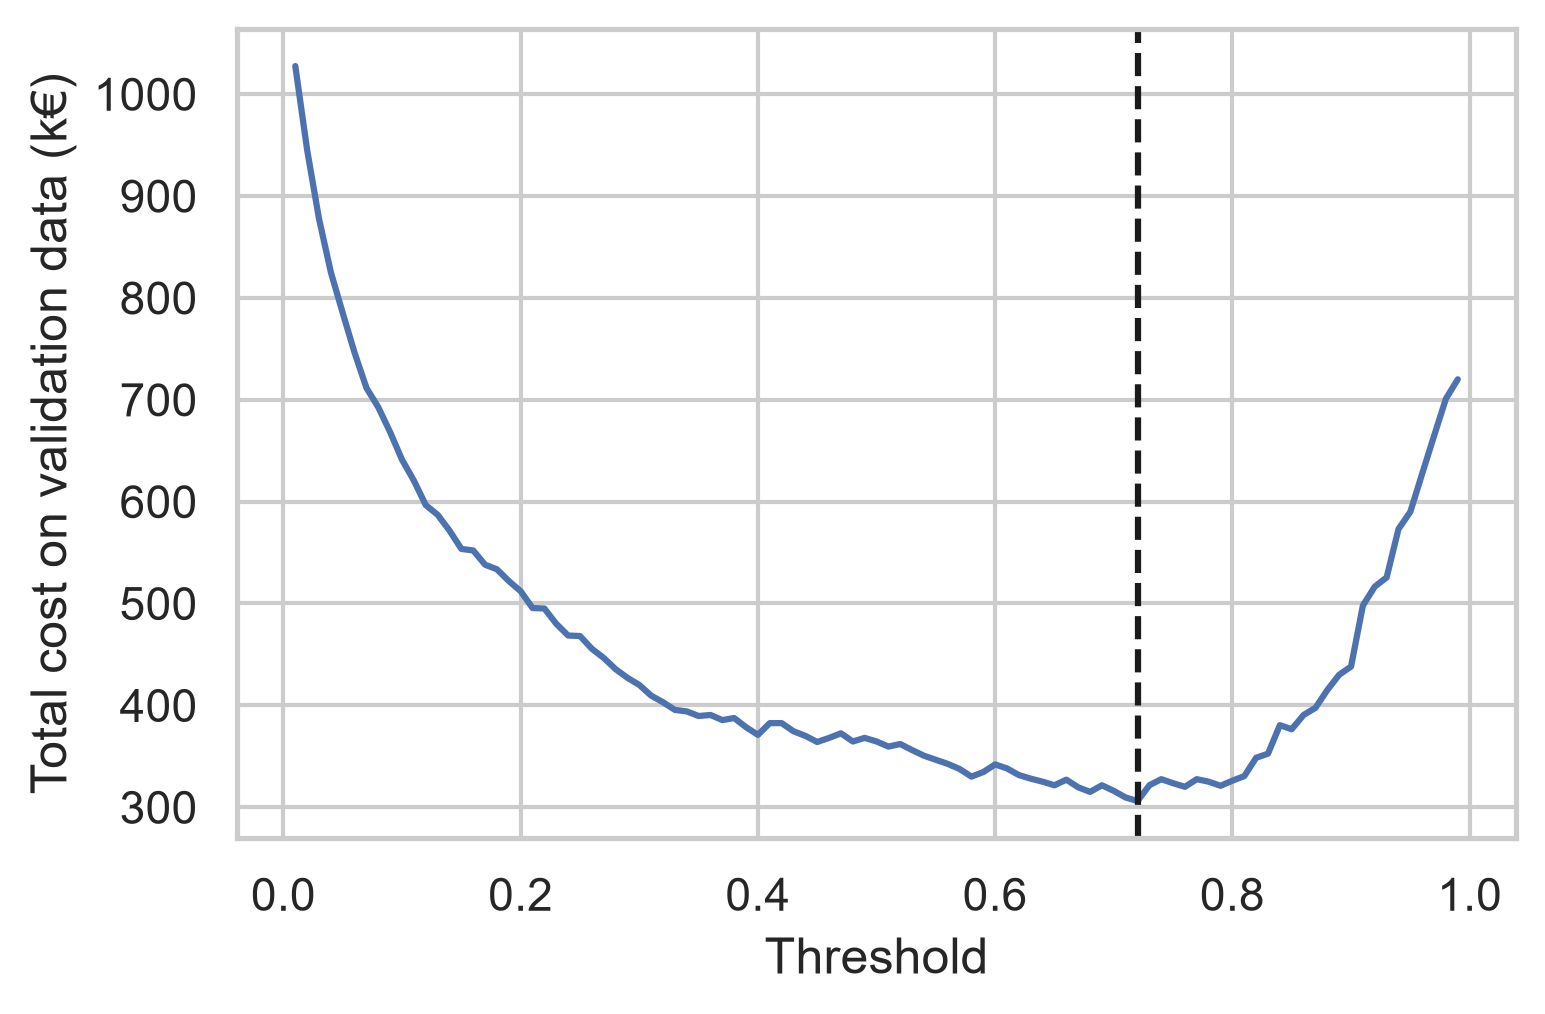
\includegraphics[keepaspectratio]{notebooks/07-classification_files/figure-pdf/cell-9-output-1.png}}

\begin{verbatim}
best threshold 0.72, cost on test data 404 k€
\end{verbatim}

The cost curve typically has a broad minimum. Note that with
\texttt{class\_weight="balanced"} the predicted probabilities are no
longer calibrated (the model behaves as if failures were as frequent as
OK records), so the optimal threshold differs from the theoretical
\(c_{FP}/(c_{FP}+c_{FN}) \approx 0.048\). Choosing the threshold on
validation data and reporting the cost on the untouched test data keeps
the evaluation honest.

\end{tcolorbox}

\begin{tcolorbox}[enhanced jigsaw, colframe=quarto-callout-caution-color-frame, toprule=.15mm, rightrule=.15mm, title=\textcolor{quarto-callout-caution-color}{\faFire}\hspace{0.5em}{Solution to Exercise 3}, colbacktitle=quarto-callout-caution-color!10!white, left=2mm, titlerule=0mm, bottomtitle=1mm, toptitle=1mm, opacityback=0, bottomrule=.15mm, breakable, arc=.35mm, opacitybacktitle=0.6, colback=white, coltitle=black, leftrule=.75mm]

\begin{Shaded}
\begin{Highlighting}[]
\ImportTok{from}\NormalTok{ sklearn.tree }\ImportTok{import}\NormalTok{ plot\_tree}

\NormalTok{tree3 }\OperatorTok{=}\NormalTok{ DecisionTreeClassifier(max\_depth}\OperatorTok{=}\DecValTok{3}\NormalTok{, class\_weight}\OperatorTok{=}\StringTok{"balanced"}\NormalTok{, random\_state}\OperatorTok{=}\DecValTok{0}\NormalTok{).fit(X\_train, y\_train)}
\NormalTok{plt.figure(figsize}\OperatorTok{=}\NormalTok{(}\DecValTok{16}\NormalTok{, }\DecValTok{7}\NormalTok{))}
\NormalTok{plot\_tree(tree3, feature\_names}\OperatorTok{=}\NormalTok{X.columns, class\_names}\OperatorTok{=}\NormalTok{[}\StringTok{"OK"}\NormalTok{, }\StringTok{"failure"}\NormalTok{], filled}\OperatorTok{=}\VariableTok{True}\NormalTok{,}
\NormalTok{          impurity}\OperatorTok{=}\VariableTok{False}\NormalTok{, proportion}\OperatorTok{=}\VariableTok{True}\NormalTok{, fontsize}\OperatorTok{=}\DecValTok{9}\NormalTok{)}
\NormalTok{plt.show()}
\end{Highlighting}
\end{Shaded}

\pandocbounded{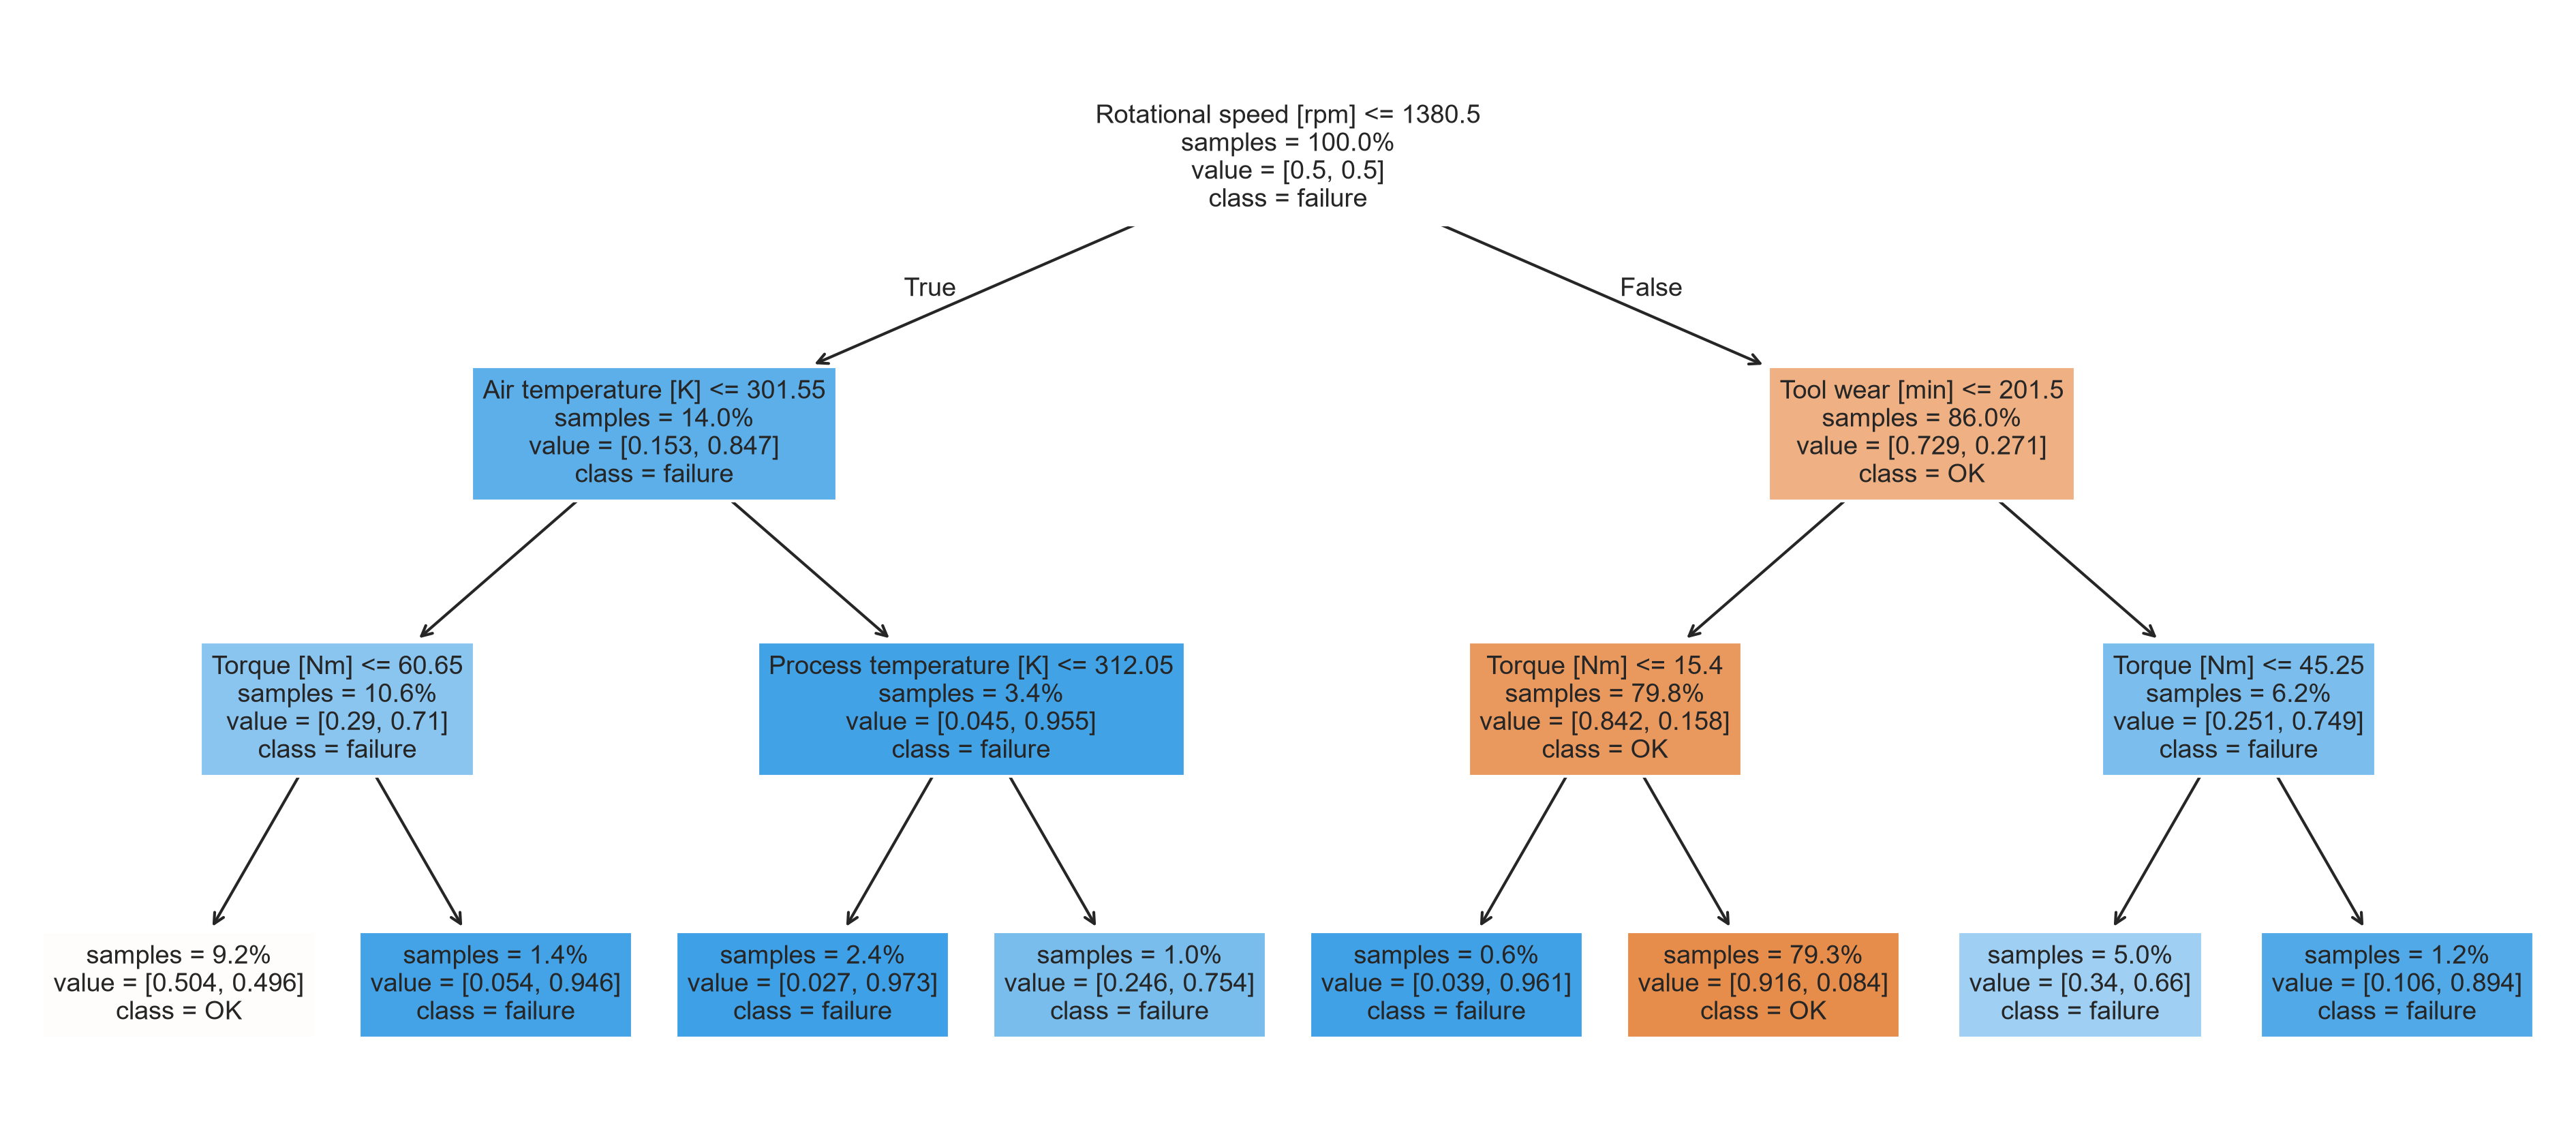
\includegraphics[keepaspectratio]{notebooks/07-classification_files/figure-pdf/cell-10-output-1.png}}

The top splits typically use torque, rotational speed and tool wear --
exactly the quantities behind the documented failure mechanisms:
overstrain (high torque × tool wear), power failure (power too low or
too high, i.e.~extreme torque--speed combinations) and tool wear failure
(large tool wear). A tree that splits mainly on product ID or random
variables would be suspicious. Checking learned rules against physics is
one of the best plausibility tests for a model.

\end{tcolorbox}

\begin{tcolorbox}[enhanced jigsaw, colframe=quarto-callout-caution-color-frame, toprule=.15mm, rightrule=.15mm, title=\textcolor{quarto-callout-caution-color}{\faFire}\hspace{0.5em}{Solution to Exercise 4}, colbacktitle=quarto-callout-caution-color!10!white, left=2mm, titlerule=0mm, bottomtitle=1mm, toptitle=1mm, opacityback=0, bottomrule=.15mm, breakable, arc=.35mm, opacitybacktitle=0.6, colback=white, coltitle=black, leftrule=.75mm]

\begin{Shaded}
\begin{Highlighting}[]
\NormalTok{X\_eng }\OperatorTok{=}\NormalTok{ X.copy()}
\NormalTok{X\_eng[}\StringTok{"power [W]"}\NormalTok{] }\OperatorTok{=}\NormalTok{ ai4i[}\StringTok{"Torque [Nm]"}\NormalTok{] }\OperatorTok{*}\NormalTok{ ai4i[}\StringTok{"Rotational speed [rpm]"}\NormalTok{] }\OperatorTok{*} \DecValTok{2} \OperatorTok{*}\NormalTok{ np.pi }\OperatorTok{/} \DecValTok{60}
\NormalTok{X\_eng[}\StringTok{"delta T [K]"}\NormalTok{] }\OperatorTok{=}\NormalTok{ ai4i[}\StringTok{"Process temperature [K]"}\NormalTok{] }\OperatorTok{{-}}\NormalTok{ ai4i[}\StringTok{"Air temperature [K]"}\NormalTok{]}
\NormalTok{X\_eng[}\StringTok{"strain [min Nm]"}\NormalTok{] }\OperatorTok{=}\NormalTok{ ai4i[}\StringTok{"Tool wear [min]"}\NormalTok{] }\OperatorTok{*}\NormalTok{ ai4i[}\StringTok{"Torque [Nm]"}\NormalTok{]}

\ImportTok{from}\NormalTok{ sklearn.model\_selection }\ImportTok{import}\NormalTok{ cross\_val\_score, StratifiedKFold}
\NormalTok{skf }\OperatorTok{=}\NormalTok{ StratifiedKFold(}\DecValTok{5}\NormalTok{, shuffle}\OperatorTok{=}\VariableTok{True}\NormalTok{, random\_state}\OperatorTok{=}\DecValTok{0}\NormalTok{)}
\ControlFlowTok{for}\NormalTok{ name, data }\KeywordTok{in}\NormalTok{ [(}\StringTok{"original features"}\NormalTok{, X), (}\StringTok{"with engineered features"}\NormalTok{, X\_eng)]:}
\NormalTok{    s }\OperatorTok{=}\NormalTok{ cross\_val\_score(make\_pipeline(StandardScaler(), LogisticRegression(class\_weight}\OperatorTok{=}\StringTok{"balanced"}\NormalTok{, max\_iter}\OperatorTok{=}\DecValTok{2000}\NormalTok{)),}
\NormalTok{                        data, y, cv}\OperatorTok{=}\NormalTok{skf, scoring}\OperatorTok{=}\StringTok{"average\_precision"}\NormalTok{)}
    \BuiltInTok{print}\NormalTok{(}\SpecialStringTok{f"}\SpecialCharTok{\{}\NormalTok{name}\SpecialCharTok{:26s\}}\SpecialStringTok{ average precision = }\SpecialCharTok{\{}\NormalTok{s}\SpecialCharTok{.}\NormalTok{mean()}\SpecialCharTok{:.3f\}}\SpecialStringTok{"}\NormalTok{)}
\end{Highlighting}
\end{Shaded}

\begin{verbatim}
original features          average precision = 0.429
with engineered features   average precision = 0.453
\end{verbatim}

Engineered features based on physics can help logistic regression a lot,
because they turn curved boundaries into simpler ones. But power
failures occur for \emph{both} too low and too high power -- a linear
model in \texttt{power} can only represent one side. Squared or binned
terms, or a tree-based model, are needed to capture both. This is a
typical example of how domain knowledge and model choice interact.

\end{tcolorbox}

\begin{tcolorbox}[enhanced jigsaw, colframe=quarto-callout-caution-color-frame, toprule=.15mm, rightrule=.15mm, title=\textcolor{quarto-callout-caution-color}{\faFire}\hspace{0.5em}{Solution to Exercise 5}, colbacktitle=quarto-callout-caution-color!10!white, left=2mm, titlerule=0mm, bottomtitle=1mm, toptitle=1mm, opacityback=0, bottomrule=.15mm, breakable, arc=.35mm, opacitybacktitle=0.6, colback=white, coltitle=black, leftrule=.75mm]

Total = 1000. Accuracy = (950 + 15)/1000 = 96.5 \%. Precision = 15/(15 +
30) = 33 \%. Recall = 15/(15 + 5) = 75 \%. F1 = 2 · 0.33 · 0.75/(0.33 +
0.75) ≈ 0.46.

The accuracy is lower than that of the trivial model ``always OK'' (98
\%)! Still, the model may be useful: it detects three of four failures,
at the price of two false alarms per real one. Whether that is
acceptable depends on the costs -- if a missed failure is expensive and
checking an alarm is cheap, this model is valuable despite its ``bad''
accuracy.

\end{tcolorbox}

\chapter{Ensembles and
Interpretability}\label{ensembles-and-interpretability}

A single decision tree is easy to understand but a poor predictor: it
overfits, and a small change in the data can produce a completely
different tree. The remedy is surprisingly simple -- combine many trees.
\textbf{Ensemble methods} such as random forests and gradient boosting
are, for tabular data, among the most accurate general-purpose methods
available. In industrial practice they are often the first choice for
quality prediction, fault classification and virtual sensors.

Their accuracy comes at a price: an ensemble of hundreds of trees is no
longer transparent. Yet engineers need to know \emph{why} a model
predicts a defect -- to trust it, to check it against physics and to
derive process improvements. The second half of this chapter therefore
introduces methods to interpret such models.

\textbf{Scenario: which defects can be classified automatically?}

The automatic inspection line of a steel mill detects surface defects
reliably, but a human inspector still has to assign every defect to a
defect class -- the class decides whether a plate is reworked,
downgraded or scrapped. The inspectors are overloaded. The quality
manager proposes to let a model classify those defect classes it
recognises reliably and to send only the rest to the inspectors.
``Reliable'' means: precision and recall of at least 90 \% for that
class.

\textbf{Your decision:} Which defect classes may be classified
automatically, and how much inspector workload does that save?

\textbf{Learning goals.} After this chapter you can

\begin{itemize}
\tightlist
\item
  explain bagging and boosting and why they improve on a single tree,
\item
  train random forests and gradient boosting models and tune their
  hyperparameters with cross-validated search,
\item
  solve and evaluate multi-class problems,
\item
  interpret models with permutation importance and partial dependence
  plots, knowing their limitations,
\item
  (extension) explain individual predictions with SHAP values.
\end{itemize}

\textbf{Datasets in this chapter}

\begin{itemize}
\tightlist
\item
  \href{https://archive.ics.uci.edu/dataset/198/steel+plates+faults}{Steel
  Plates Faults (UCI)}
\end{itemize}

\section{Why ensembles work}\label{why-ensembles-work}

Recall the bias--variance decomposition from Chapter 6. A deep decision
tree has low bias but high variance. If we could average many trees
trained on \emph{different} datasets from the same process, the variance
would shrink while the bias stays low. Ensembles approximate this idea
in two different ways.

\begin{figure}[H]

\centering{

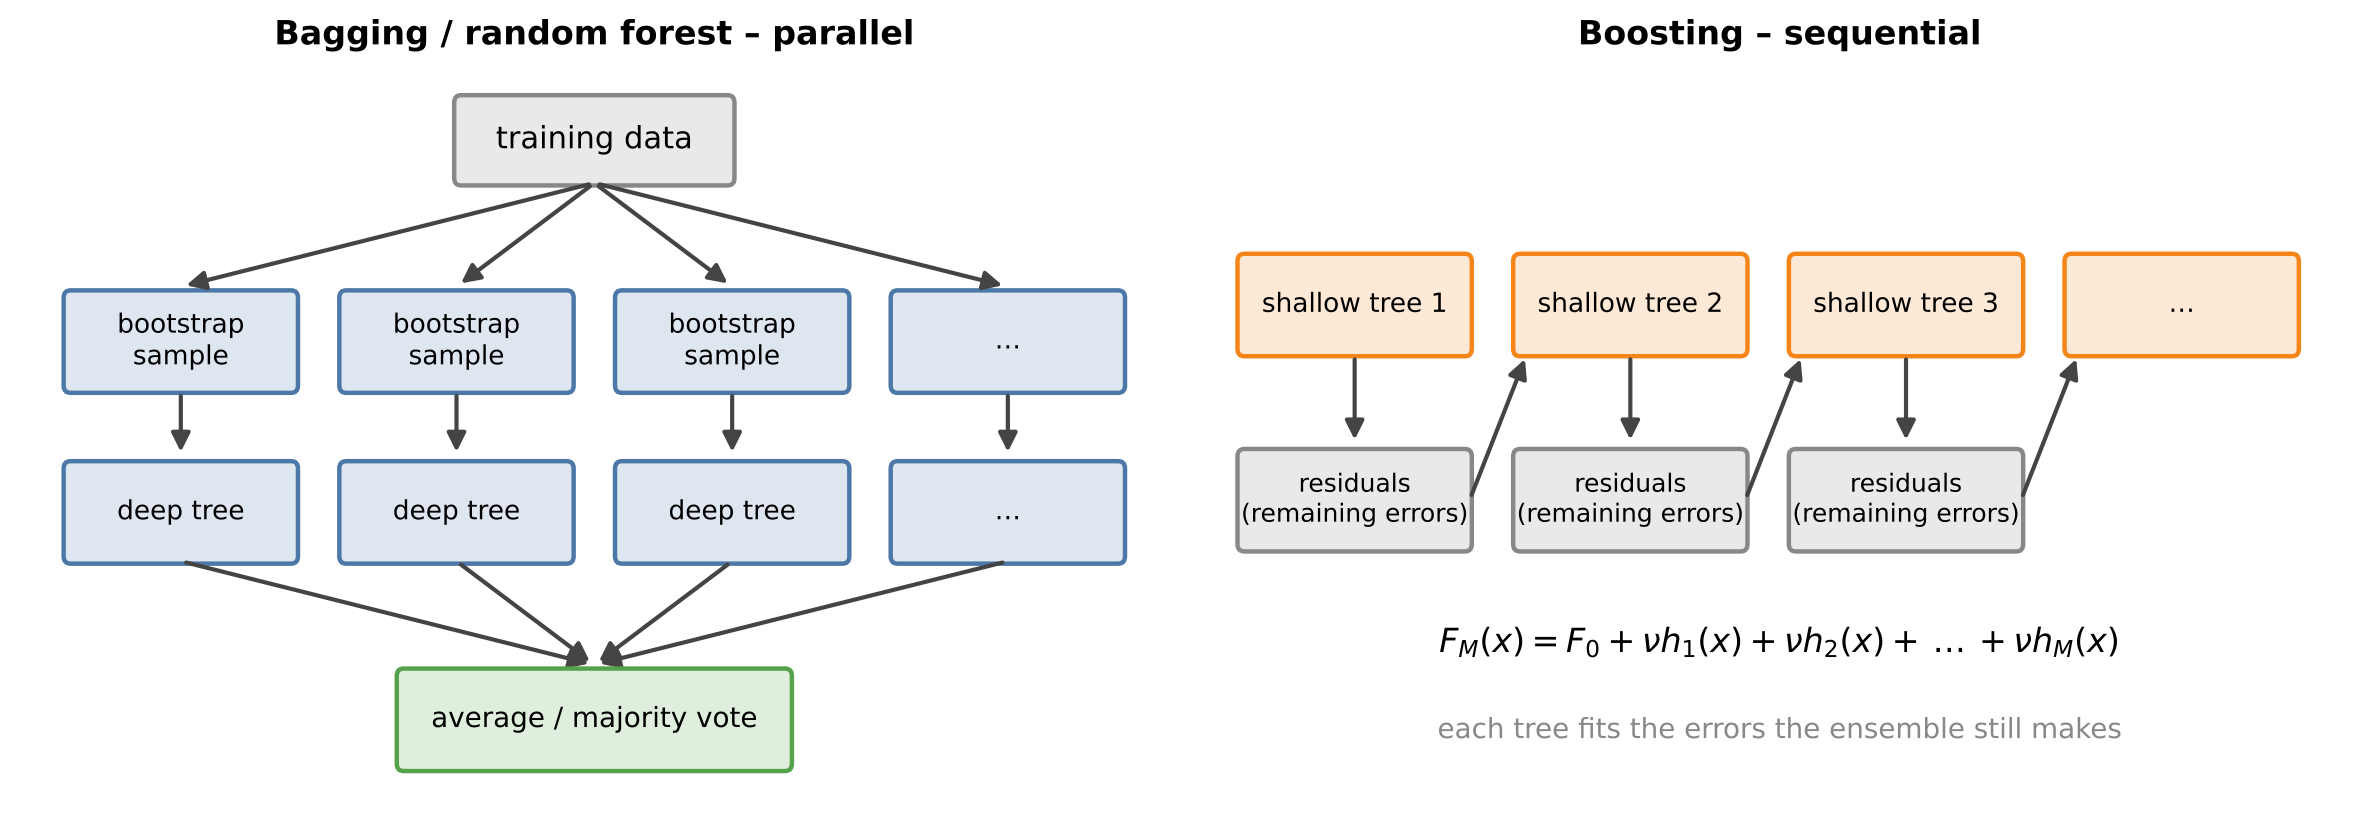
\includegraphics[width=1\linewidth,height=\textheight,keepaspectratio]{notebooks/images/bagging-boosting.png}

}

\caption{\label{fig-ensembles}Bagging and boosting. Bagging trains many
deep trees independently on bootstrap samples and averages them
(variance reduction). Boosting trains shallow trees one after another,
each one correcting the remaining errors of the ensemble so far (bias
reduction).}

\end{figure}%

\subsection{Bagging and random
forests}\label{bagging-and-random-forests}

\begin{tcolorbox}[enhanced jigsaw, colframe=quarto-callout-note-color-frame, toprule=.15mm, rightrule=.15mm, title=\textcolor{quarto-callout-note-color}{\faInfo}\hspace{0.5em}{Definition: Bagging and random forest}, colbacktitle=quarto-callout-note-color!10!white, left=2mm, titlerule=0mm, bottomtitle=1mm, toptitle=1mm, opacityback=0, bottomrule=.15mm, breakable, arc=.35mm, opacitybacktitle=0.6, colback=white, coltitle=black, leftrule=.75mm]

\textbf{Bagging} (bootstrap aggregating) trains \(B\) models on \(B\)
bootstrap samples of the training data and averages their predictions
(regression) or takes a majority vote (classification). A \textbf{random
forest} is bagging with decision trees plus one additional trick: at
each split, only a random subset of the features (e.g.~\(\sqrt{p}\) of
\(p\) features) is considered. This decorrelates the trees and makes the
averaging more effective.

\end{tcolorbox}

Why the extra randomness helps: averaging \(B\) predictions with
variance \(\sigma^2\) and pairwise correlation \(\rho\) gives a variance
of \(\rho\sigma^2 + \frac{1-\rho}{B}\sigma^2\). More trees reduce only
the second term; reducing the correlation \(\rho\) between the trees
reduces the first. Random forests have few critical hyperparameters,
rarely overfit when more trees are added, and provide a free validation
estimate: each tree did not see about a third of the data
(\emph{out-of-bag} samples), on which it can be evaluated.

\subsection{Boosting}\label{boosting}

\begin{tcolorbox}[enhanced jigsaw, colframe=quarto-callout-note-color-frame, toprule=.15mm, rightrule=.15mm, title=\textcolor{quarto-callout-note-color}{\faInfo}\hspace{0.5em}{Definition: Gradient boosting}, colbacktitle=quarto-callout-note-color!10!white, left=2mm, titlerule=0mm, bottomtitle=1mm, toptitle=1mm, opacityback=0, bottomrule=.15mm, breakable, arc=.35mm, opacitybacktitle=0.6, colback=white, coltitle=black, leftrule=.75mm]

Gradient boosting builds the model step by step:
\[F_m(x) = F_{m-1}(x) + \nu\, h_m(x),\] where each new tree \(h_m\) is
fitted to the negative gradient of the loss with respect to the current
predictions -- for squared error simply the \textbf{residuals} of
\(F_{m-1}\). The \textbf{learning rate} \(0 < \nu \le 1\) shrinks each
step.

\end{tcolorbox}

Boosting uses shallow trees (depth 3--8) that individually are weak, and
reduces mainly the bias. Unlike random forests, boosting \emph{can}
overfit if too many trees are added; the number of trees, the learning
rate and the tree depth must be tuned together, typically with early
stopping on validation data. Modern implementations (scikit-learn's
\texttt{HistGradientBoostingClassifier}, XGBoost, LightGBM) are very
fast and handle missing values natively.

\begin{tcolorbox}[enhanced jigsaw, colframe=quarto-callout-tip-color-frame, toprule=.15mm, rightrule=.15mm, title=\textcolor{quarto-callout-tip-color}{\faLightbulb}\hspace{0.5em}{Engineering practice: which method first?}, colbacktitle=quarto-callout-tip-color!10!white, left=2mm, titlerule=0mm, bottomtitle=1mm, toptitle=1mm, opacityback=0, bottomrule=.15mm, breakable, arc=.35mm, opacitybacktitle=0.6, colback=white, coltitle=black, leftrule=.75mm]

For a new tabular problem, a random forest with default settings is a
robust first model that needs almost no tuning. Gradient boosting is
often a few percent more accurate but requires tuning. A linear or
logistic model remains the essential baseline -- if the ensemble is only
marginally better, the simpler model may be preferable for transparency.

\end{tcolorbox}

\section{Multi-class problems}\label{multi-class-problems}

With \(K > 2\) classes, the confusion matrix becomes \(K \times K\), and
precision and recall are computed per class. They can be averaged in two
ways: the \textbf{macro} average treats every class equally (important
if rare classes matter), the \textbf{weighted} average weights them by
their frequency. Balanced accuracy is the macro average of the recalls.

\section{Interpreting models}\label{interpreting-models}

\begin{tcolorbox}[enhanced jigsaw, colframe=quarto-callout-note-color-frame, toprule=.15mm, rightrule=.15mm, title=\textcolor{quarto-callout-note-color}{\faInfo}\hspace{0.5em}{Definition: Permutation importance}, colbacktitle=quarto-callout-note-color!10!white, left=2mm, titlerule=0mm, bottomtitle=1mm, toptitle=1mm, opacityback=0, bottomrule=.15mm, breakable, arc=.35mm, opacitybacktitle=0.6, colback=white, coltitle=black, leftrule=.75mm]

The importance of feature \(j\) is the decrease in a performance score
(on validation or test data) when the values of feature \(j\) are
randomly shuffled, which destroys its relationship with the target while
keeping its distribution.

\end{tcolorbox}

Permutation importance works for any model. The impurity-based
\texttt{feature\_importances\_} of tree models are cheaper but biased
towards features with many distinct values and computed on training
data.

\begin{tcolorbox}[enhanced jigsaw, colframe=quarto-callout-warning-color-frame, toprule=.15mm, rightrule=.15mm, title=\textcolor{quarto-callout-warning-color}{\faExclamationTriangle}\hspace{0.5em}{Pitfall: importance is not causality -- and correlated features share
importance}, colbacktitle=quarto-callout-warning-color!10!white, left=2mm, titlerule=0mm, bottomtitle=1mm, toptitle=1mm, opacityback=0, bottomrule=.15mm, breakable, arc=.35mm, opacitybacktitle=0.6, colback=white, coltitle=black, leftrule=.75mm]

A high importance means that the \emph{model} relies on a feature, not
that the feature \emph{causes} the defect. If two features are strongly
correlated (e.g.~two dimensions of a defect), shuffling one of them
hurts little because the other still carries the information -- both may
appear unimportant although the information is essential.

\end{tcolorbox}

A \textbf{partial dependence plot} (PDP) shows how the predicted
probability changes on average when one feature is varied over its range
while the others keep their observed values. It answers the engineering
question ``in which direction and how strongly does this measurement
influence the prediction?'' and reveals thresholds and nonlinearities.

\begin{Shaded}
\begin{Highlighting}[]
\CommentTok{\# Setup: works locally and in Google Colab}
\ImportTok{import}\NormalTok{ importlib.util, subprocess, sys}
\ControlFlowTok{for}\NormalTok{ pkg }\KeywordTok{in}\NormalTok{ [}\StringTok{"ucimlrepo"}\NormalTok{, }\StringTok{"shap"}\NormalTok{]:}
    \ControlFlowTok{if}\NormalTok{ importlib.util.find\_spec(pkg) }\KeywordTok{is} \VariableTok{None}\NormalTok{:}
\NormalTok{        subprocess.run([sys.executable, }\StringTok{"{-}m"}\NormalTok{, }\StringTok{"pip"}\NormalTok{, }\StringTok{"install"}\NormalTok{, }\StringTok{"{-}q"}\NormalTok{, pkg], check}\OperatorTok{=}\VariableTok{True}\NormalTok{)}

\ImportTok{import}\NormalTok{ numpy }\ImportTok{as}\NormalTok{ np}
\ImportTok{import}\NormalTok{ pandas }\ImportTok{as}\NormalTok{ pd}
\ImportTok{import}\NormalTok{ matplotlib.pyplot }\ImportTok{as}\NormalTok{ plt}
\ImportTok{import}\NormalTok{ seaborn }\ImportTok{as}\NormalTok{ sns}

\NormalTok{sns.set\_theme(style}\OperatorTok{=}\StringTok{"whitegrid"}\NormalTok{)}
\end{Highlighting}
\end{Shaded}

\section{Live coding: steel plate
faults}\label{live-coding-steel-plate-faults}

The dataset comes from the automatic inspection of steel plates. For
1,941 detected surface defects, 27 features were extracted from the
inspection images and the production data: position and size of the
defect (\texttt{X\_Minimum}, \texttt{Pixels\_Areas},
\texttt{Length\_of\_Conveyer}, \ldots), luminosity statistics, shape
indices, the steel type and the plate thickness. Each defect belongs to
one of seven classes: \emph{Pastry}, \emph{Z\_Scratch},
\emph{K\_Scatch}, \emph{Stains}, \emph{Dirtiness}, \emph{Bumps} and
\emph{Other\_Faults}.

\begin{Shaded}
\begin{Highlighting}[]
\ImportTok{from}\NormalTok{ ucimlrepo }\ImportTok{import}\NormalTok{ fetch\_ucirepo}

\NormalTok{steel }\OperatorTok{=}\NormalTok{ fetch\_ucirepo(}\BuiltInTok{id}\OperatorTok{=}\DecValTok{198}\NormalTok{)}
\NormalTok{X }\OperatorTok{=}\NormalTok{ steel.data.features}
\NormalTok{y }\OperatorTok{=}\NormalTok{ steel.data.targets.idxmax(axis}\OperatorTok{=}\DecValTok{1}\NormalTok{)      }\CommentTok{\# 7 one{-}hot columns {-}\textgreater{} one label}
\NormalTok{y.value\_counts()}
\end{Highlighting}
\end{Shaded}

\begin{verbatim}
Other_Faults    673
Bumps           402
K_Scratch       391
Z_Scratch       190
Pastry          158
Stains           72
Dirtiness        55
Name: count, dtype: int64
\end{verbatim}

The classes are imbalanced: \emph{Other\_Faults} is by far the largest
class, while \emph{Dirtiness} and \emph{Stains} are rare. ``Other
faults'' is a heterogeneous rest category -- we must expect it to be
hard to classify.

\begin{Shaded}
\begin{Highlighting}[]
\ImportTok{from}\NormalTok{ sklearn.model\_selection }\ImportTok{import}\NormalTok{ train\_test\_split, cross\_val\_score, StratifiedKFold}
\ImportTok{from}\NormalTok{ sklearn.ensemble }\ImportTok{import}\NormalTok{ RandomForestClassifier, HistGradientBoostingClassifier}
\ImportTok{from}\NormalTok{ sklearn.linear\_model }\ImportTok{import}\NormalTok{ LogisticRegression}
\ImportTok{from}\NormalTok{ sklearn.pipeline }\ImportTok{import}\NormalTok{ make\_pipeline}
\ImportTok{from}\NormalTok{ sklearn.preprocessing }\ImportTok{import}\NormalTok{ StandardScaler}

\NormalTok{X\_train, X\_test, y\_train, y\_test }\OperatorTok{=}\NormalTok{ train\_test\_split(X, y, test\_size}\OperatorTok{=}\FloatTok{0.25}\NormalTok{, stratify}\OperatorTok{=}\NormalTok{y, random\_state}\OperatorTok{=}\DecValTok{0}\NormalTok{)}
\NormalTok{cv }\OperatorTok{=}\NormalTok{ StratifiedKFold(}\DecValTok{5}\NormalTok{, shuffle}\OperatorTok{=}\VariableTok{True}\NormalTok{, random\_state}\OperatorTok{=}\DecValTok{0}\NormalTok{)}

\NormalTok{candidates }\OperatorTok{=}\NormalTok{ \{}
    \StringTok{"logistic regression (baseline)"}\NormalTok{: make\_pipeline(StandardScaler(), LogisticRegression(max\_iter}\OperatorTok{=}\DecValTok{3000}\NormalTok{)),}
    \StringTok{"random forest"}\NormalTok{: RandomForestClassifier(n\_estimators}\OperatorTok{=}\DecValTok{300}\NormalTok{, random\_state}\OperatorTok{=}\DecValTok{0}\NormalTok{, n\_jobs}\OperatorTok{={-}}\DecValTok{1}\NormalTok{),}
    \StringTok{"gradient boosting"}\NormalTok{: HistGradientBoostingClassifier(random\_state}\OperatorTok{=}\DecValTok{0}\NormalTok{),}
\NormalTok{\}}
\ControlFlowTok{for}\NormalTok{ name, m }\KeywordTok{in}\NormalTok{ candidates.items():}
\NormalTok{    s }\OperatorTok{=}\NormalTok{ cross\_val\_score(m, X\_train, y\_train, cv}\OperatorTok{=}\NormalTok{cv, scoring}\OperatorTok{=}\StringTok{"balanced\_accuracy"}\NormalTok{)}
    \BuiltInTok{print}\NormalTok{(}\SpecialStringTok{f"}\SpecialCharTok{\{}\NormalTok{name}\SpecialCharTok{:32s\}}\SpecialStringTok{ balanced accuracy = }\SpecialCharTok{\{}\NormalTok{s}\SpecialCharTok{.}\NormalTok{mean()}\SpecialCharTok{:.3f\}}\SpecialStringTok{ ± }\SpecialCharTok{\{}\NormalTok{s}\SpecialCharTok{.}\NormalTok{std()}\SpecialCharTok{:.3f\}}\SpecialStringTok{"}\NormalTok{)}
\end{Highlighting}
\end{Shaded}

\begin{verbatim}
logistic regression (baseline)   balanced accuracy = 0.717 ± 0.019
random forest                    balanced accuracy = 0.750 ± 0.019
gradient boosting                balanced accuracy = 0.785 ± 0.022
\end{verbatim}

\textbf{Discussion.} Both ensembles should clearly outperform the
logistic regression baseline. The standard deviation across folds
indicates how much of the difference between the ensembles is real --
differences smaller than this spread should not be over-interpreted.
With seven classes, guessing would reach a balanced accuracy of about
1/7 ≈ 0.14.

\begin{Shaded}
\begin{Highlighting}[]
\ImportTok{from}\NormalTok{ sklearn.metrics }\ImportTok{import}\NormalTok{ classification\_report, ConfusionMatrixDisplay}

\NormalTok{rf }\OperatorTok{=}\NormalTok{ candidates[}\StringTok{"random forest"}\NormalTok{].fit(X\_train, y\_train)}
\BuiltInTok{print}\NormalTok{(classification\_report(y\_test, rf.predict(X\_test), digits}\OperatorTok{=}\DecValTok{3}\NormalTok{))}
\NormalTok{ConfusionMatrixDisplay.from\_estimator(rf, X\_test, y\_test, xticks\_rotation}\OperatorTok{=}\DecValTok{45}\NormalTok{, colorbar}\OperatorTok{=}\VariableTok{False}\NormalTok{,}
\NormalTok{                                      normalize}\OperatorTok{=}\StringTok{"true"}\NormalTok{, values\_format}\OperatorTok{=}\StringTok{".2f"}\NormalTok{)}
\NormalTok{plt.show()}
\end{Highlighting}
\end{Shaded}

\begin{verbatim}
              precision    recall  f1-score   support

       Bumps      0.771     0.733     0.751       101
   Dirtiness      0.833     0.714     0.769        14
   K_Scratch      0.967     0.908     0.937        98
Other_Faults      0.692     0.804     0.744       168
      Pastry      0.656     0.538     0.592        39
      Stains      1.000     0.944     0.971        18
   Z_Scratch      0.929     0.812     0.867        48

    accuracy                          0.792       486
   macro avg      0.836     0.779     0.804       486
weighted avg      0.800     0.792     0.793       486
\end{verbatim}

\pandocbounded{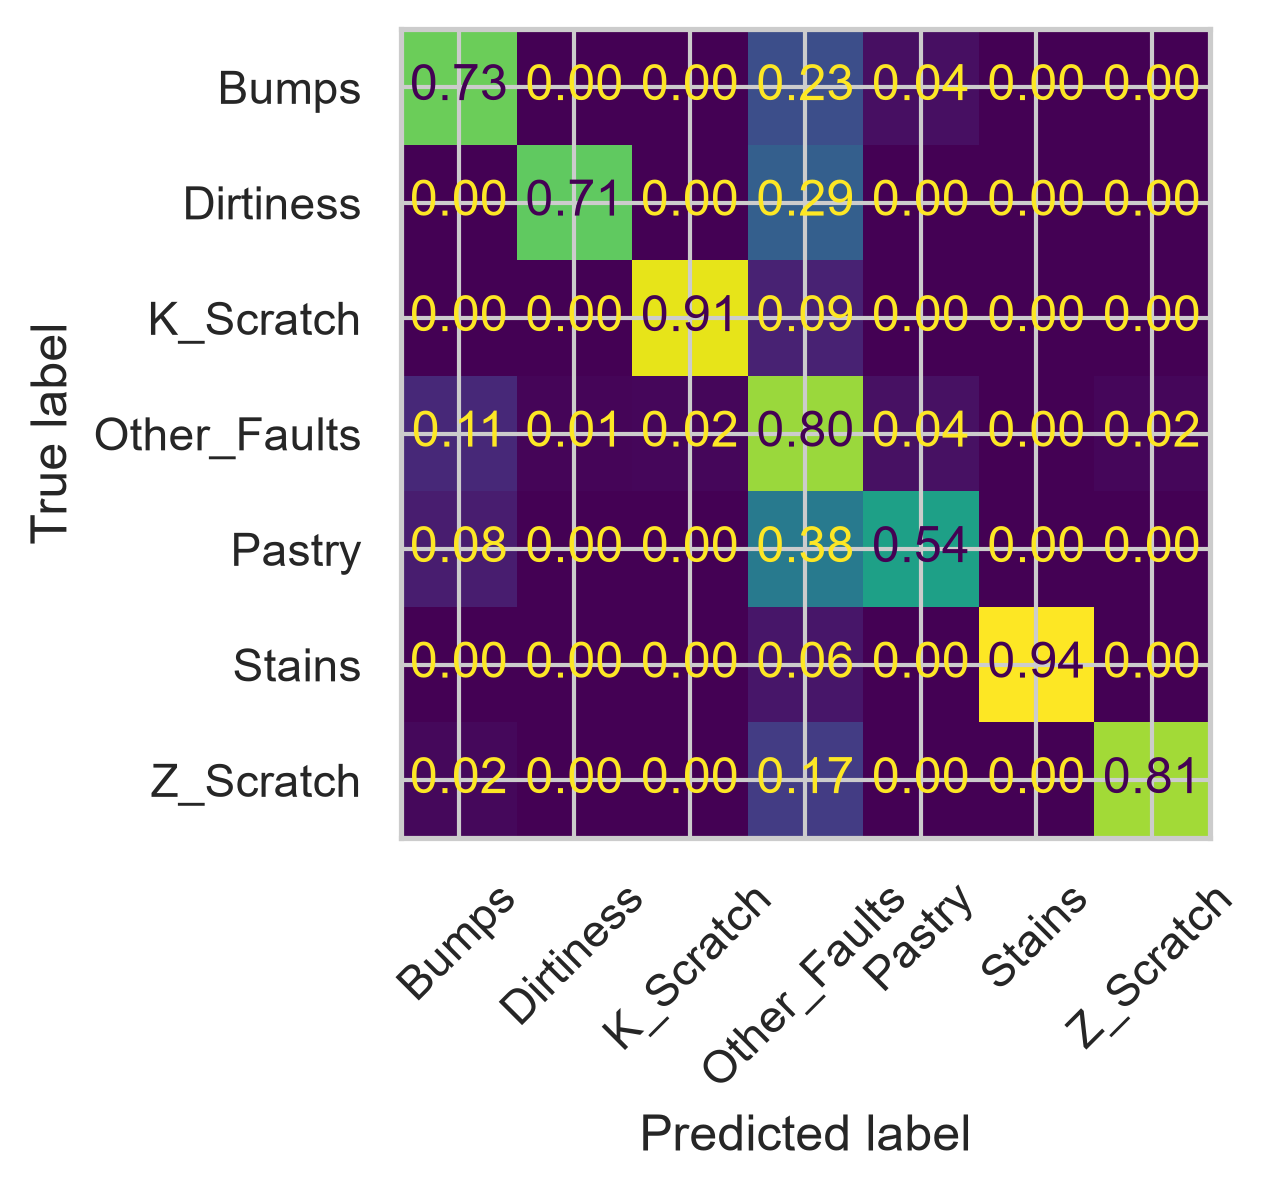
\includegraphics[keepaspectratio]{notebooks/08-ensembles_files/figure-pdf/cell-5-output-2.png}}

The row-normalised confusion matrix shows for each true class where its
defects end up. Typically, geometrically distinctive defects (scratches,
pastry) are recognised well, while \emph{Other\_Faults} and \emph{Bumps}
are confused with each other.

\begin{Shaded}
\begin{Highlighting}[]
\ImportTok{from}\NormalTok{ sklearn.inspection }\ImportTok{import}\NormalTok{ permutation\_importance}

\NormalTok{pi }\OperatorTok{=}\NormalTok{ permutation\_importance(rf, X\_test, y\_test, n\_repeats}\OperatorTok{=}\DecValTok{10}\NormalTok{, random\_state}\OperatorTok{=}\DecValTok{0}\NormalTok{,}
\NormalTok{                            scoring}\OperatorTok{=}\StringTok{"balanced\_accuracy"}\NormalTok{)}
\NormalTok{imp }\OperatorTok{=}\NormalTok{ pd.Series(pi.importances\_mean, index}\OperatorTok{=}\NormalTok{X.columns).sort\_values()}
\NormalTok{imp.tail(}\DecValTok{10}\NormalTok{).plot.barh(xlabel}\OperatorTok{=}\StringTok{"Drop in balanced accuracy when shuffled"}\NormalTok{)}
\NormalTok{plt.show()}
\end{Highlighting}
\end{Shaded}

\pandocbounded{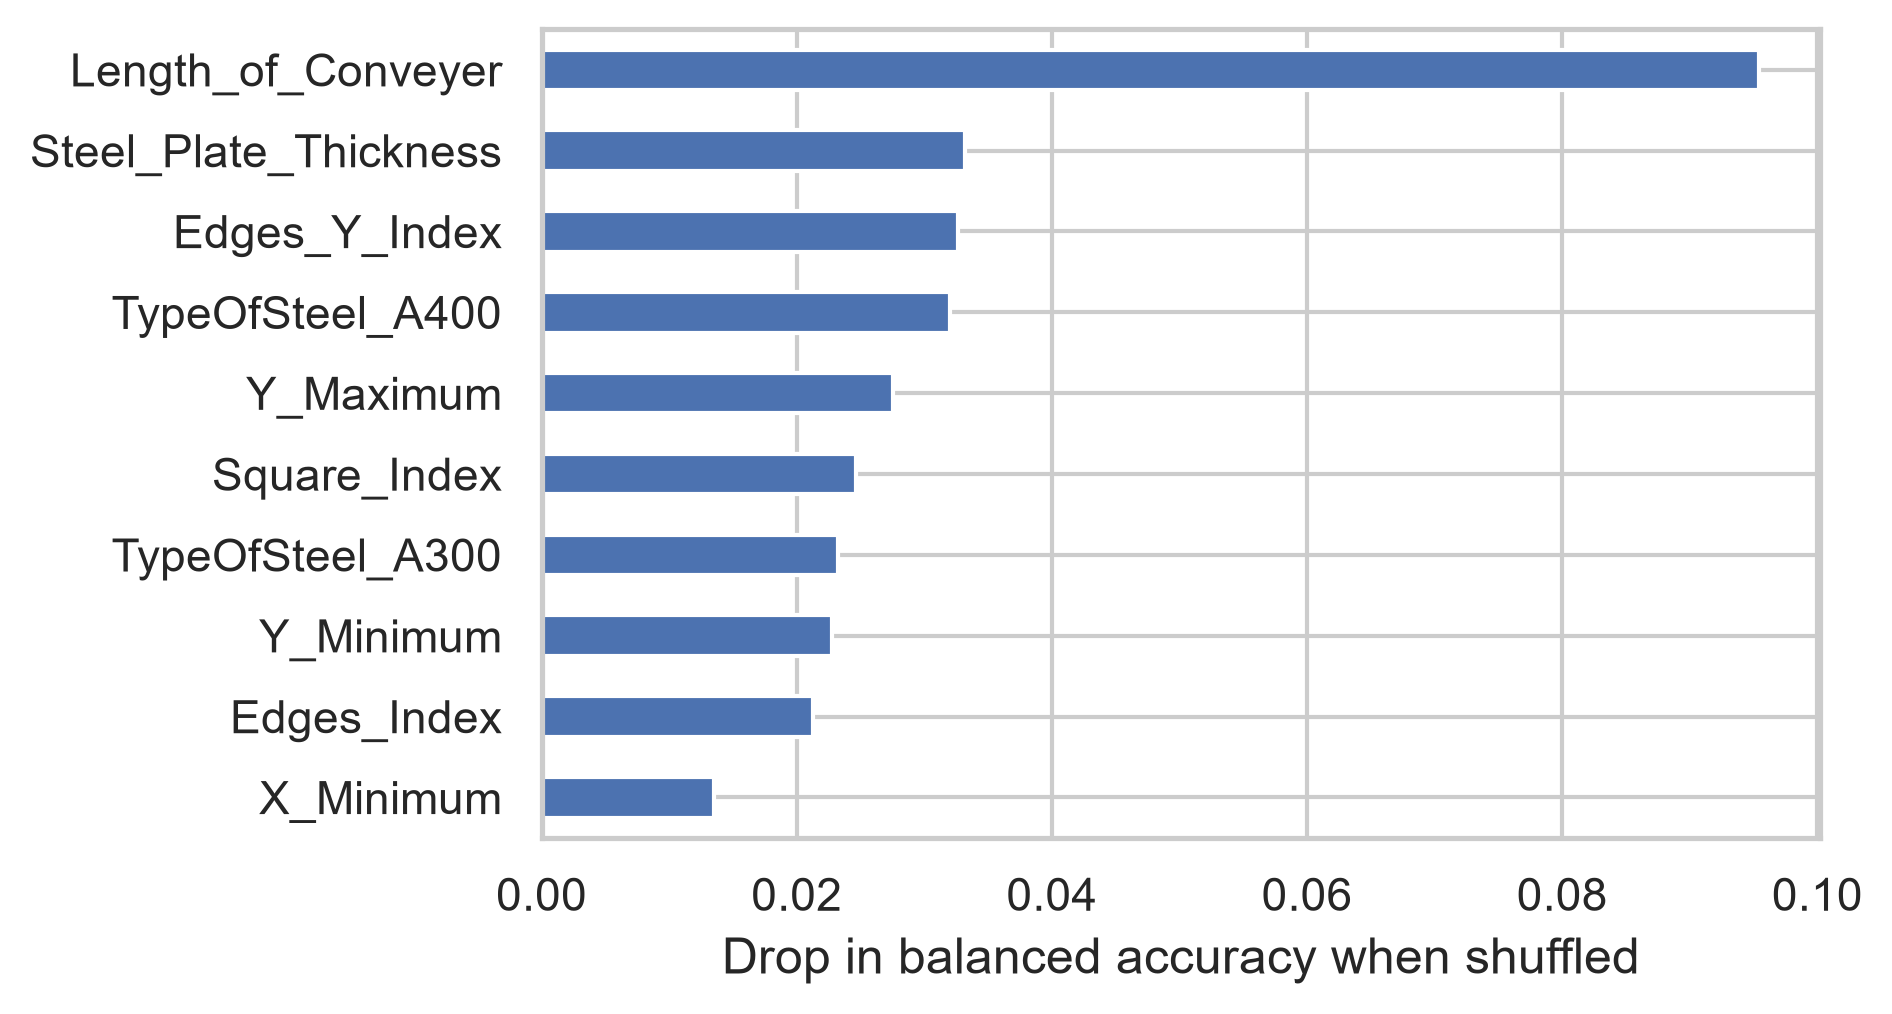
\includegraphics[keepaspectratio]{notebooks/08-ensembles_files/figure-pdf/cell-6-output-1.png}}

\begin{Shaded}
\begin{Highlighting}[]
\ImportTok{from}\NormalTok{ sklearn.inspection }\ImportTok{import}\NormalTok{ PartialDependenceDisplay}

\CommentTok{\# The most important feature with a continuous range of values (binary features such as}
\CommentTok{\# the steel type have no meaningful curve). Partial dependence needs floating{-}point data.}
\NormalTok{top }\OperatorTok{=} \BuiltInTok{next}\NormalTok{(c }\ControlFlowTok{for}\NormalTok{ c }\KeywordTok{in}\NormalTok{ imp.index[::}\OperatorTok{{-}}\DecValTok{1}\NormalTok{] }\ControlFlowTok{if}\NormalTok{ X\_test[c].nunique() }\OperatorTok{\textgreater{}} \DecValTok{10}\NormalTok{)}
\BuiltInTok{print}\NormalTok{(}\StringTok{"Feature:"}\NormalTok{, top)}
\NormalTok{PartialDependenceDisplay.from\_estimator(rf, X\_test.astype(}\BuiltInTok{float}\NormalTok{), [top], target}\OperatorTok{=}\NormalTok{rf.classes\_[}\DecValTok{0}\NormalTok{], kind}\OperatorTok{=}\StringTok{"average"}\NormalTok{)}
\NormalTok{plt.title(}\SpecialStringTok{f"Partial dependence for class \textquotesingle{}}\SpecialCharTok{\{}\NormalTok{rf}\SpecialCharTok{.}\NormalTok{classes\_[}\DecValTok{0}\NormalTok{]}\SpecialCharTok{\}}\SpecialStringTok{\textquotesingle{}"}\NormalTok{)}
\NormalTok{plt.show()}
\end{Highlighting}
\end{Shaded}

\begin{verbatim}
Feature: Length_of_Conveyer
\end{verbatim}

\pandocbounded{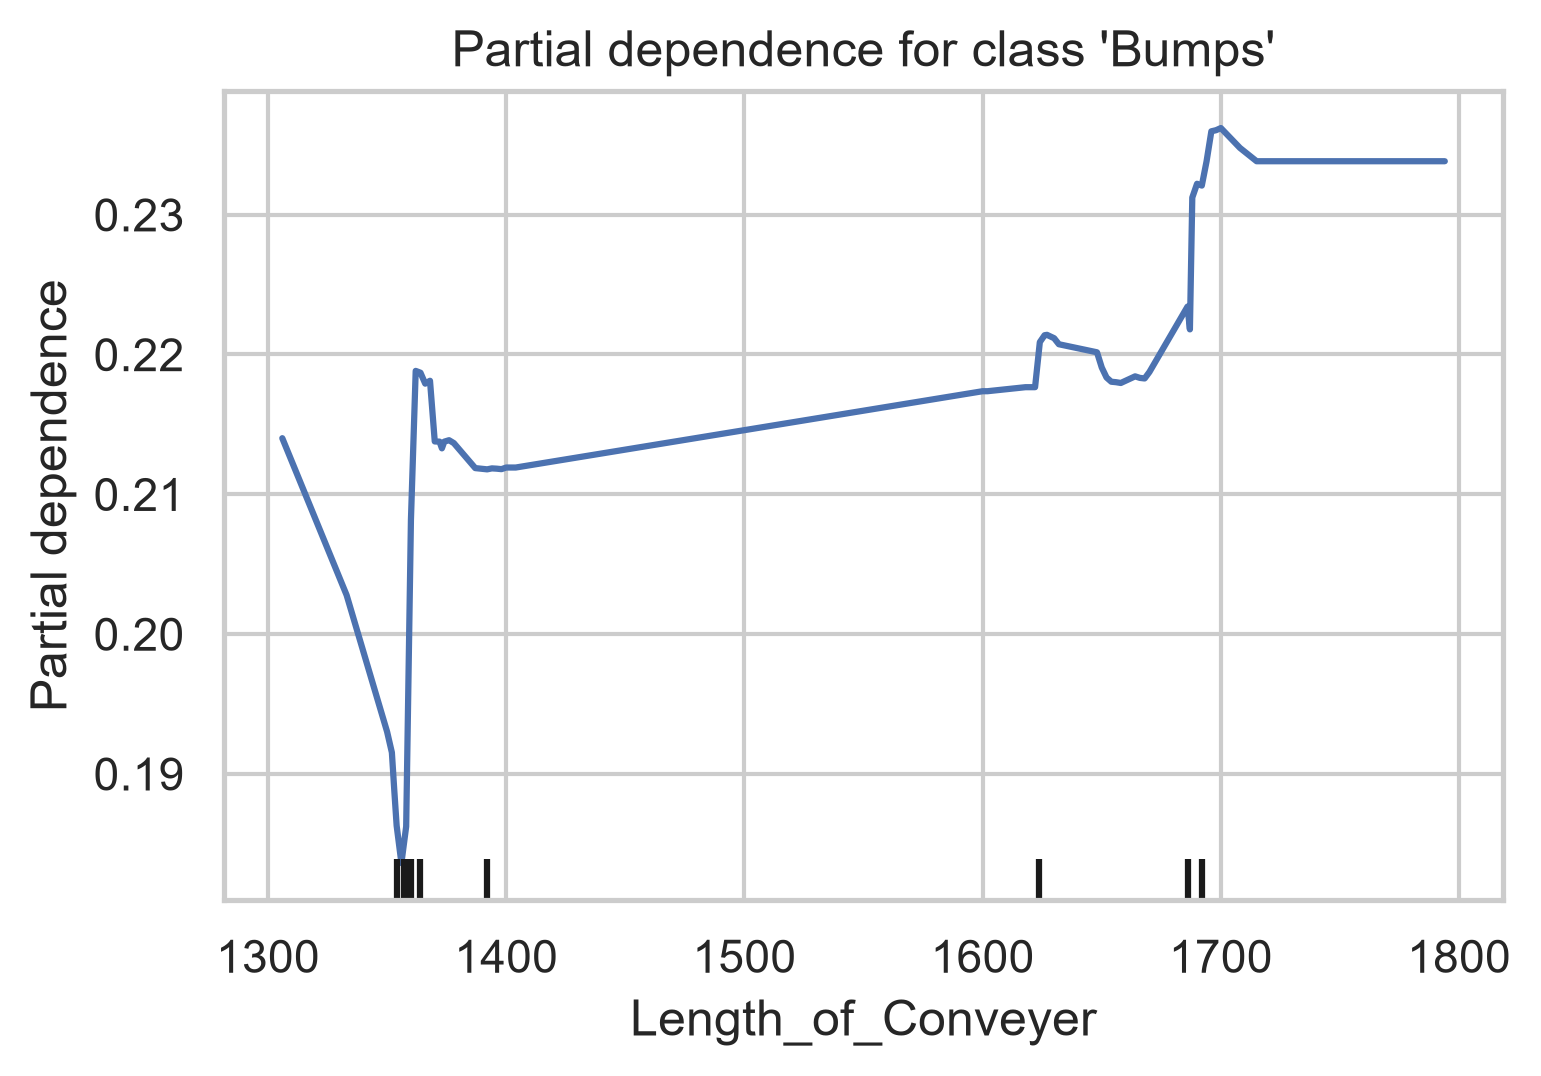
\includegraphics[keepaspectratio]{notebooks/08-ensembles_files/figure-pdf/cell-7-output-2.png}}

\textbf{Discussion.} The importance ranking tells us which measurements
the model relies on -- for steel defects typically luminosity and
geometry features as well as the steel type and plate thickness. The
partial dependence plot shows \emph{how} the predicted probability of
one class changes along the most important continuous feature. Look for
thresholds: a steep step suggests a physical limit or a property of the
inspection system worth discussing with the process engineers.

\section{Back to the decision}\label{back-to-the-decision-7}

For each class we need both high precision (when the model says
``scratch'', it really is one) and high recall (it finds the scratches).
We read both from the test set and apply the 90 \% criterion.

\begin{Shaded}
\begin{Highlighting}[]
\ImportTok{from}\NormalTok{ sklearn.metrics }\ImportTok{import}\NormalTok{ precision\_recall\_fscore\_support}

\NormalTok{prec, rec, \_, support }\OperatorTok{=}\NormalTok{ precision\_recall\_fscore\_support(y\_test, rf.predict(X\_test), labels}\OperatorTok{=}\NormalTok{rf.classes\_, zero\_division}\OperatorTok{=}\DecValTok{0}\NormalTok{)}
\NormalTok{per\_class }\OperatorTok{=}\NormalTok{ pd.DataFrame(\{}\StringTok{"precision"}\NormalTok{: prec, }\StringTok{"recall"}\NormalTok{: rec, }\StringTok{"test cases"}\NormalTok{: support\}, index}\OperatorTok{=}\NormalTok{rf.classes\_)}
\NormalTok{per\_class[}\StringTok{"automate"}\NormalTok{] }\OperatorTok{=}\NormalTok{ (per\_class[}\StringTok{"precision"}\NormalTok{] }\OperatorTok{\textgreater{}=} \FloatTok{0.9}\NormalTok{) }\OperatorTok{\&}\NormalTok{ (per\_class[}\StringTok{"recall"}\NormalTok{] }\OperatorTok{\textgreater{}=} \FloatTok{0.9}\NormalTok{)}
\BuiltInTok{print}\NormalTok{(per\_class.}\BuiltInTok{round}\NormalTok{(}\DecValTok{2}\NormalTok{))}
\NormalTok{share }\OperatorTok{=}\NormalTok{ per\_class.loc[per\_class[}\StringTok{"automate"}\NormalTok{], }\StringTok{"test cases"}\NormalTok{].}\BuiltInTok{sum}\NormalTok{() }\OperatorTok{/}\NormalTok{ per\_class[}\StringTok{"test cases"}\NormalTok{].}\BuiltInTok{sum}\NormalTok{()}
\NormalTok{auto }\OperatorTok{=} \BuiltInTok{list}\NormalTok{(per\_class.index[per\_class[}\StringTok{"automate"}\NormalTok{]])}
\BuiltInTok{print}\NormalTok{(}\SpecialStringTok{f"Decision: automate }\SpecialCharTok{\{}\NormalTok{auto }\ControlFlowTok{if}\NormalTok{ auto }\ControlFlowTok{else} \StringTok{\textquotesingle{}no class yet\textquotesingle{}}\SpecialCharTok{\}}\SpecialStringTok{ – about }\SpecialCharTok{\{}\NormalTok{share}\SpecialCharTok{:.0\%\}}\SpecialStringTok{ of the defects would no longer need an inspector."}\NormalTok{)}
\end{Highlighting}
\end{Shaded}

\begin{verbatim}
              precision  recall  test cases  automate
Bumps              0.77    0.73         101     False
Dirtiness          0.83    0.71          14     False
K_Scratch          0.97    0.91          98      True
Other_Faults       0.69    0.80         168     False
Pastry             0.66    0.54          39     False
Stains             1.00    0.94          18      True
Z_Scratch          0.93    0.81          48     False
Decision: automate ['K_Scratch', 'Stains'] – about 24% of the defects would no longer need an inspector.
\end{verbatim}

With only a few dozen test cases per class, precision and recall are
themselves uncertain -- a class that just passes the 90 \% mark should
be monitored closely after go-live, for example by having inspectors
check a random sample of automatically classified plates. Classes that
fail the criterion are good candidates for better labels or additional
features.

\section{Extension: SHAP values}\label{extension-shap-values}

\emph{Extension -- optional material, not required for the exam.}

SHAP (\emph{SHapley Additive exPlanations}) distributes a single
prediction among the features, based on the Shapley value from
cooperative game theory: each feature receives its average marginal
contribution over all possible orders in which features could be added.
The contributions add up exactly to the difference between the
prediction and the average prediction. SHAP answers the question:
\emph{why} did the model classify \textbf{this} plate as K\_Scatch?

\begin{Shaded}
\begin{Highlighting}[]
\ImportTok{import}\NormalTok{ shap}

\NormalTok{explainer }\OperatorTok{=}\NormalTok{ shap.TreeExplainer(rf)}
\NormalTok{sv }\OperatorTok{=}\NormalTok{ explainer(X\_test.iloc[:}\DecValTok{200}\NormalTok{])}
\CommentTok{\# SHAP values for one class, e.g. "K\_Scatch"}
\NormalTok{cls }\OperatorTok{=} \BuiltInTok{list}\NormalTok{(rf.classes\_).index(}\StringTok{"K\_Scatch"}\NormalTok{) }\ControlFlowTok{if} \StringTok{"K\_Scatch"} \KeywordTok{in}\NormalTok{ rf.classes\_ }\ControlFlowTok{else} \DecValTok{0}
\BuiltInTok{print}\NormalTok{(}\StringTok{"SHAP values for class:"}\NormalTok{, rf.classes\_[cls])}
\NormalTok{shap.plots.beeswarm(sv[:, :, cls], max\_display}\OperatorTok{=}\DecValTok{10}\NormalTok{)}
\end{Highlighting}
\end{Shaded}

\begin{verbatim}
SHAP values for class: Bumps
\end{verbatim}

\pandocbounded{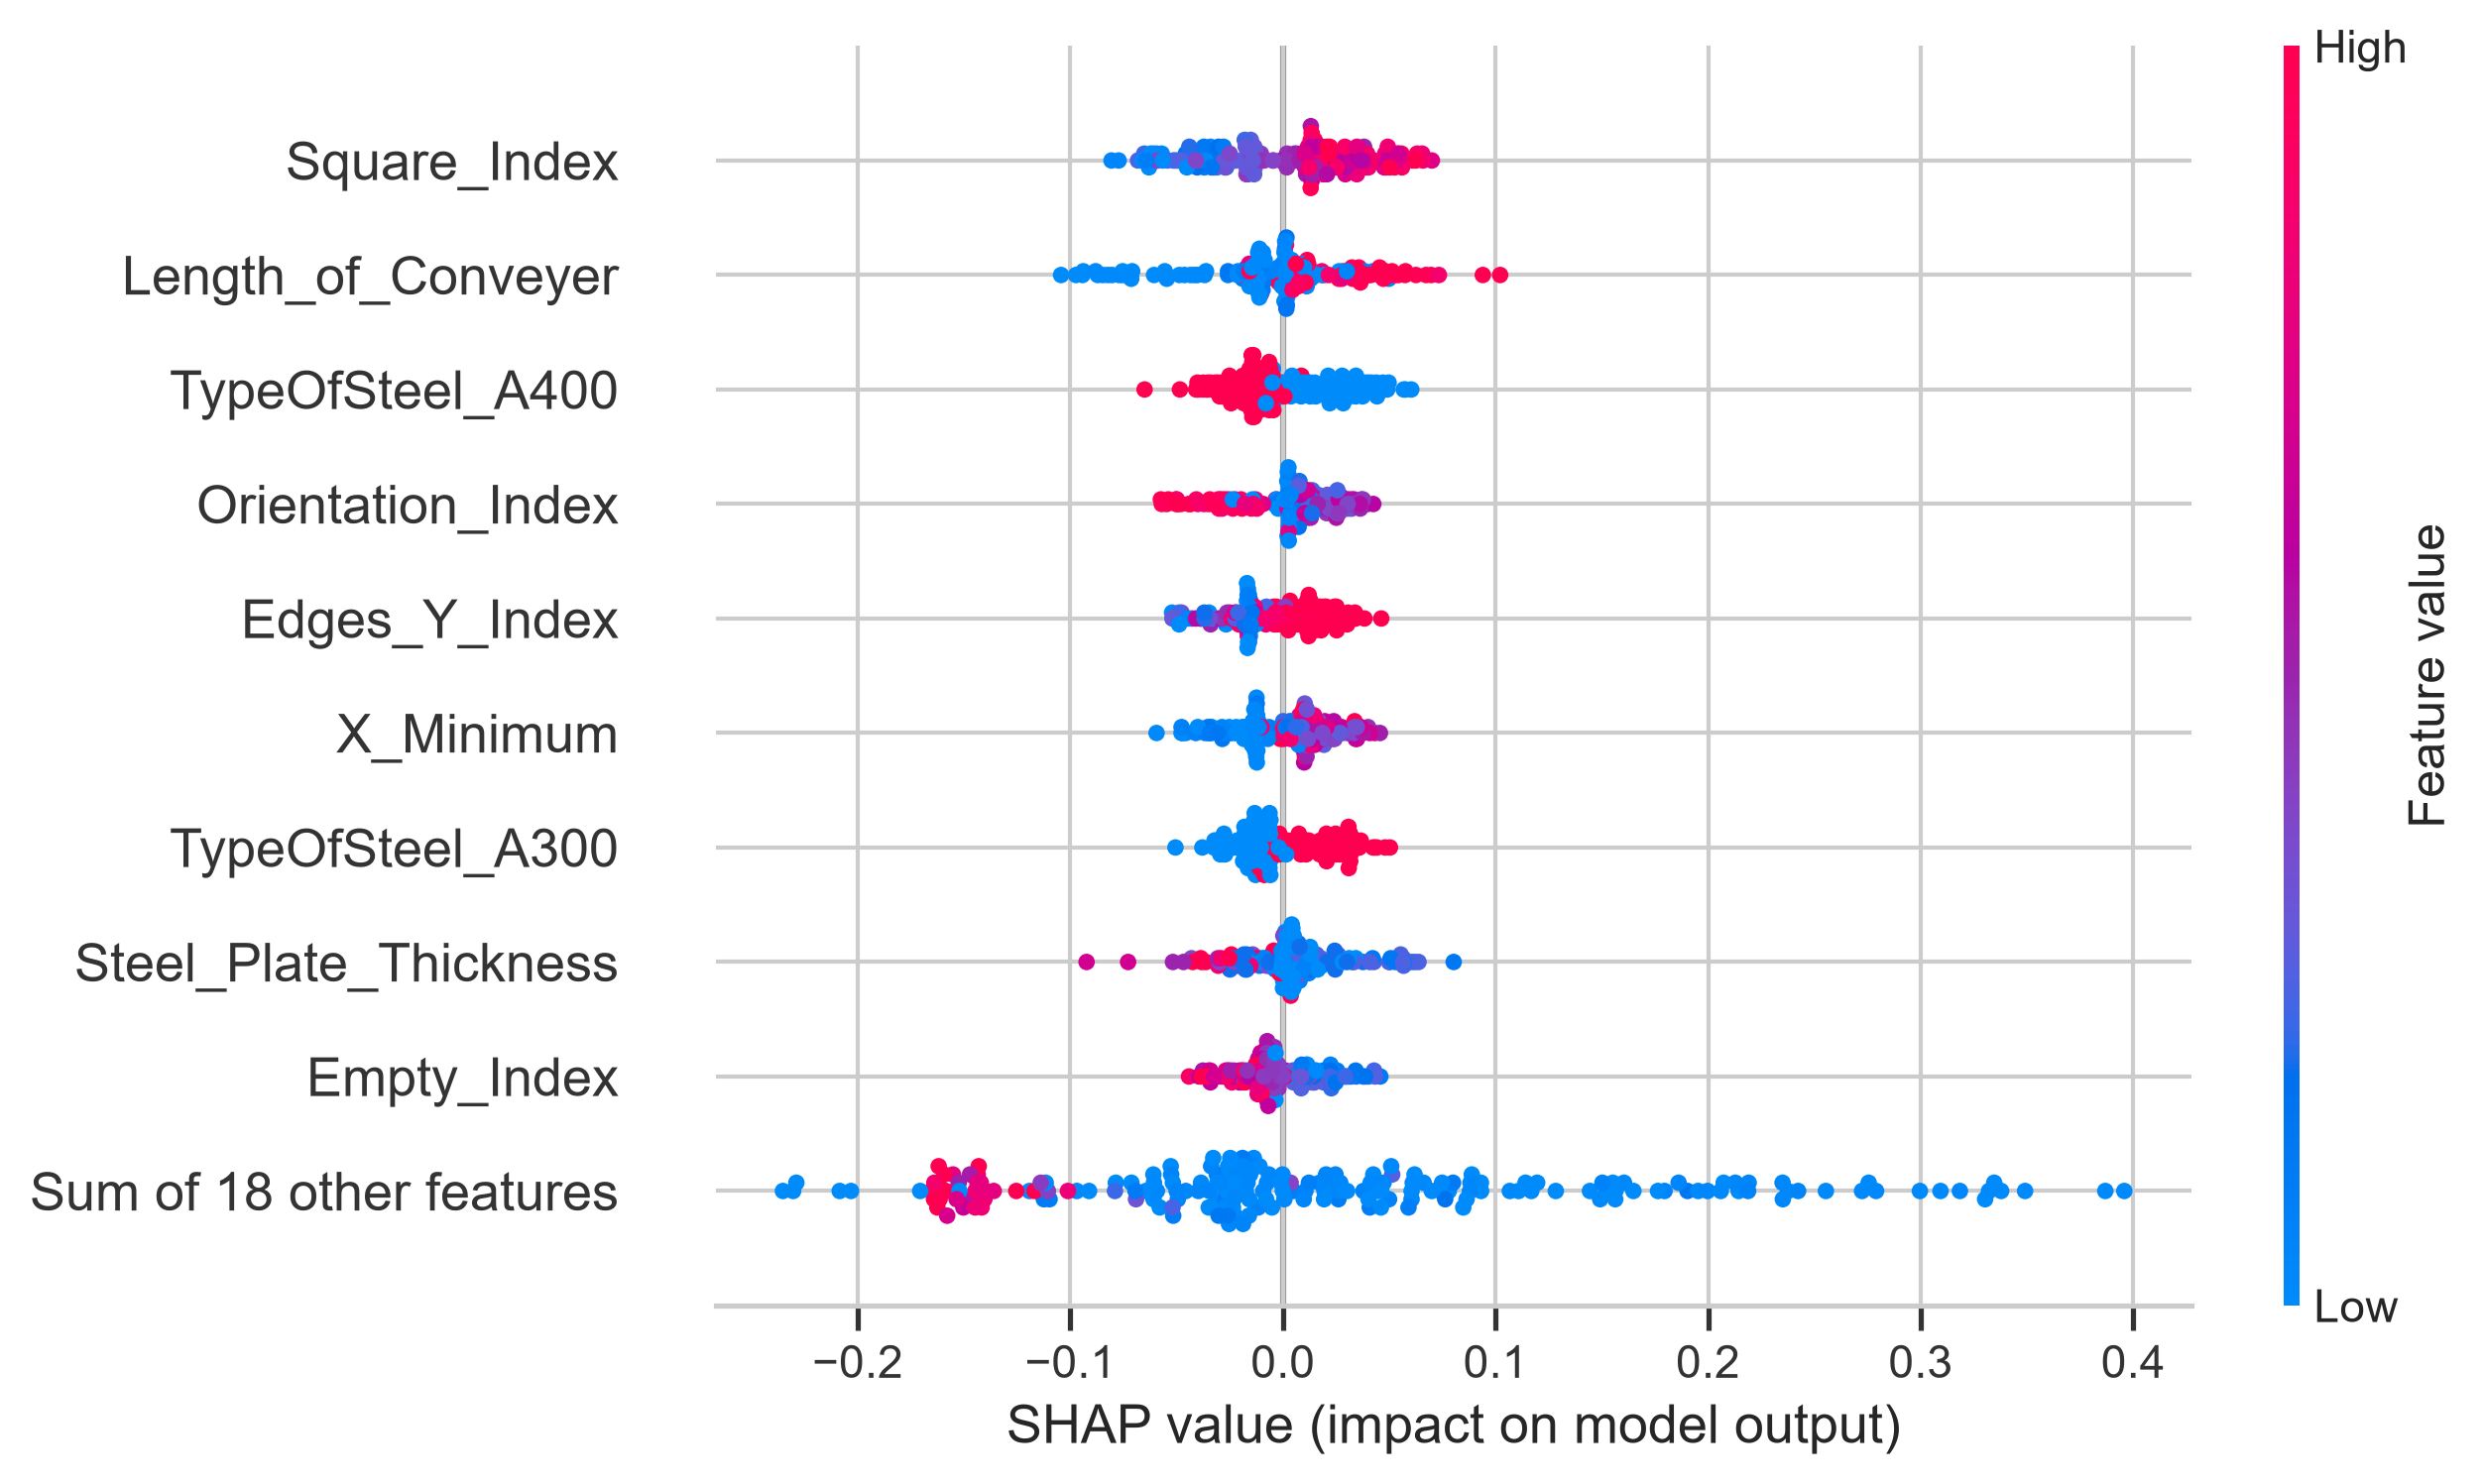
\includegraphics[keepaspectratio]{notebooks/08-ensembles_files/figure-pdf/cell-9-output-2.png}}

Each dot is one plate; its horizontal position is the contribution of
the feature to the K\_Scatch score, its colour the feature value.
Features at the top have the largest overall influence. Unlike
permutation importance, the beeswarm plot also shows the
\emph{direction} of the effect.

\begin{tcolorbox}[enhanced jigsaw, colframe=quarto-callout-important-color-frame, toprule=.15mm, rightrule=.15mm, title=\textcolor{quarto-callout-important-color}{\faExclamation}\hspace{0.5em}{Key takeaways}, colbacktitle=quarto-callout-important-color!10!white, left=2mm, titlerule=0mm, bottomtitle=1mm, toptitle=1mm, opacityback=0, bottomrule=.15mm, breakable, arc=.35mm, opacitybacktitle=0.6, colback=white, coltitle=black, leftrule=.75mm]

\begin{itemize}
\tightlist
\item
  Bagging/random forests reduce variance by averaging decorrelated deep
  trees; boosting reduces bias by adding shallow trees sequentially.
\item
  Random forests are robust defaults; gradient boosting needs tuning but
  is often slightly more accurate.
\item
  In multi-class problems, use per-class metrics and the confusion
  matrix; macro averages protect rare classes.
\item
  Permutation importance and partial dependence make black-box models
  inspectable -- but importance is not causality.
\end{itemize}

\end{tcolorbox}

\section{Exercises}\label{exercises-7}

\begin{enumerate}
\def\labelenumi{\arabic{enumi}.}
\tightlist
\item
  Tune \texttt{max\_depth}, \texttt{learning\_rate} and
  \texttt{max\_iter} of the gradient boosting model with
  \texttt{RandomizedSearchCV}. How much does the tuning gain compared
  with the default?
\item
  Which fault classes are confused most often? Look at the
  row-normalised confusion matrix and discuss whether the confusions are
  plausible.
\item
  Compare impurity-based importance (\texttt{rf.feature\_importances\_})
  with permutation importance. Why can they differ?
\item
  Train the random forest with \texttt{class\_weight="balanced"}. How do
  the recalls of the rare classes \emph{Dirtiness} and \emph{Stains}
  change?
\item
  (Extension) Explain one single prediction with a SHAP waterfall plot,
  as you would to a quality engineer.
\end{enumerate}

\subsection{Solutions}\label{solutions-7}

\begin{tcolorbox}[enhanced jigsaw, colframe=quarto-callout-caution-color-frame, toprule=.15mm, rightrule=.15mm, title=\textcolor{quarto-callout-caution-color}{\faFire}\hspace{0.5em}{Solution to Exercise 1}, colbacktitle=quarto-callout-caution-color!10!white, left=2mm, titlerule=0mm, bottomtitle=1mm, toptitle=1mm, opacityback=0, bottomrule=.15mm, breakable, arc=.35mm, opacitybacktitle=0.6, colback=white, coltitle=black, leftrule=.75mm]

\begin{Shaded}
\begin{Highlighting}[]
\ImportTok{from}\NormalTok{ sklearn.model\_selection }\ImportTok{import}\NormalTok{ RandomizedSearchCV}
\ImportTok{from}\NormalTok{ scipy.stats }\ImportTok{import}\NormalTok{ loguniform, randint}

\NormalTok{search }\OperatorTok{=}\NormalTok{ RandomizedSearchCV(}
\NormalTok{    HistGradientBoostingClassifier(random\_state}\OperatorTok{=}\DecValTok{0}\NormalTok{),}
\NormalTok{    \{}\StringTok{"learning\_rate"}\NormalTok{: loguniform(}\FloatTok{0.01}\NormalTok{, }\FloatTok{0.3}\NormalTok{), }\StringTok{"max\_depth"}\NormalTok{: randint(}\DecValTok{2}\NormalTok{, }\DecValTok{10}\NormalTok{),}
     \StringTok{"max\_iter"}\NormalTok{: randint(}\DecValTok{100}\NormalTok{, }\DecValTok{600}\NormalTok{), }\StringTok{"l2\_regularization"}\NormalTok{: loguniform(}\FloatTok{1e{-}4}\NormalTok{, }\DecValTok{1}\NormalTok{)\},}
\NormalTok{    n\_iter}\OperatorTok{=}\DecValTok{25}\NormalTok{, cv}\OperatorTok{=}\NormalTok{cv, scoring}\OperatorTok{=}\StringTok{"balanced\_accuracy"}\NormalTok{, random\_state}\OperatorTok{=}\DecValTok{0}\NormalTok{, n\_jobs}\OperatorTok{={-}}\DecValTok{1}\NormalTok{)}
\NormalTok{search.fit(X\_train, y\_train)}
\BuiltInTok{print}\NormalTok{(}\StringTok{"best parameters:"}\NormalTok{, search.best\_params\_)}
\BuiltInTok{print}\NormalTok{(}\SpecialStringTok{f"CV balanced accuracy: tuned }\SpecialCharTok{\{}\NormalTok{search}\SpecialCharTok{.}\NormalTok{best\_score\_}\SpecialCharTok{:.3f\}}\SpecialStringTok{"}\NormalTok{)}
\end{Highlighting}
\end{Shaded}

\begin{verbatim}
best parameters: {'l2_regularization': np.float64(0.028079081078857277), 'learning_rate': np.float64(0.0815241575370242), 'max_depth': 9, 'max_iter': 488}
CV balanced accuracy: tuned 0.783
\end{verbatim}

Random search samples hyperparameter combinations instead of trying a
full grid -- usually more efficient when only a few parameters matter.
The gain over the default is often modest (a few percentage points);
compare it with the fold-to-fold standard deviation before concluding
that tuning was worthwhile. The CV score of the best configuration is
slightly optimistic, because it was selected among 25 candidates -- an
untouched test set gives the honest estimate.

\end{tcolorbox}

\begin{tcolorbox}[enhanced jigsaw, colframe=quarto-callout-caution-color-frame, toprule=.15mm, rightrule=.15mm, title=\textcolor{quarto-callout-caution-color}{\faFire}\hspace{0.5em}{Solution to Exercise 2}, colbacktitle=quarto-callout-caution-color!10!white, left=2mm, titlerule=0mm, bottomtitle=1mm, toptitle=1mm, opacityback=0, bottomrule=.15mm, breakable, arc=.35mm, opacitybacktitle=0.6, colback=white, coltitle=black, leftrule=.75mm]

The largest off-diagonal entries of the normalised confusion matrix show
the most frequent confusions. Typically, \emph{Other\_Faults} is
confused with \emph{Bumps} and vice versa: both are less distinct in
shape, and ``other'' is a collection of different defect types without a
common signature. Geometrically clear defects such as \emph{K\_Scatch}
or \emph{Pastry} are rarely confused. From a process point of view,
refining the \emph{Other\_Faults} category (better labels) may improve
the classification more than any change of the algorithm.

\end{tcolorbox}

\begin{tcolorbox}[enhanced jigsaw, colframe=quarto-callout-caution-color-frame, toprule=.15mm, rightrule=.15mm, title=\textcolor{quarto-callout-caution-color}{\faFire}\hspace{0.5em}{Solution to Exercise 3}, colbacktitle=quarto-callout-caution-color!10!white, left=2mm, titlerule=0mm, bottomtitle=1mm, toptitle=1mm, opacityback=0, bottomrule=.15mm, breakable, arc=.35mm, opacitybacktitle=0.6, colback=white, coltitle=black, leftrule=.75mm]

\begin{Shaded}
\begin{Highlighting}[]
\BuiltInTok{cmp} \OperatorTok{=}\NormalTok{ pd.DataFrame(\{}\StringTok{"impurity"}\NormalTok{: pd.Series(rf.feature\_importances\_, index}\OperatorTok{=}\NormalTok{X.columns),}
                    \StringTok{"permutation"}\NormalTok{: imp\})}
\BuiltInTok{cmp}\NormalTok{.rank(ascending}\OperatorTok{=}\VariableTok{False}\NormalTok{).sort\_values(}\StringTok{"permutation"}\NormalTok{).head(}\DecValTok{10}\NormalTok{)}
\end{Highlighting}
\end{Shaded}

\begin{longtable}[]{@{}lll@{}}
\toprule\noalign{}
& impurity & permutation \\
\midrule\noalign{}
\endhead
\bottomrule\noalign{}
\endlastfoot
Length\_of\_Conveyer & 2.0 & 1.0 \\
Steel\_Plate\_Thickness & 6.0 & 2.0 \\
Edges\_Y\_Index & 18.0 & 3.0 \\
TypeOfSteel\_A400 & 25.0 & 4.0 \\
Y\_Maximum & 17.0 & 5.0 \\
Square\_Index & 14.0 & 6.0 \\
TypeOfSteel\_A300 & 26.0 & 7.0 \\
Y\_Minimum & 19.0 & 8.0 \\
Edges\_Index & 13.0 & 9.0 \\
X\_Minimum & 8.0 & 10.0 \\
\end{longtable}

Impurity importance is computed on the training data during tree
building and favours continuous features with many possible split
points; it also distributes importance over correlated features.
Permutation importance is computed on test data and measures what the
model actually needs for its predictions. Strongly correlated features
(e.g.~different measures of the defect size) can have high impurity
importance but low permutation importance, because shuffling one leaves
the others intact.

\end{tcolorbox}

\begin{tcolorbox}[enhanced jigsaw, colframe=quarto-callout-caution-color-frame, toprule=.15mm, rightrule=.15mm, title=\textcolor{quarto-callout-caution-color}{\faFire}\hspace{0.5em}{Solution to Exercise 4}, colbacktitle=quarto-callout-caution-color!10!white, left=2mm, titlerule=0mm, bottomtitle=1mm, toptitle=1mm, opacityback=0, bottomrule=.15mm, breakable, arc=.35mm, opacitybacktitle=0.6, colback=white, coltitle=black, leftrule=.75mm]

\begin{Shaded}
\begin{Highlighting}[]
\ImportTok{from}\NormalTok{ sklearn.metrics }\ImportTok{import}\NormalTok{ recall\_score}

\NormalTok{rf\_bal }\OperatorTok{=}\NormalTok{ RandomForestClassifier(n\_estimators}\OperatorTok{=}\DecValTok{300}\NormalTok{, class\_weight}\OperatorTok{=}\StringTok{"balanced"}\NormalTok{, random\_state}\OperatorTok{=}\DecValTok{0}\NormalTok{, n\_jobs}\OperatorTok{={-}}\DecValTok{1}\NormalTok{)}
\NormalTok{rf\_bal.fit(X\_train, y\_train)}
\NormalTok{pd.DataFrame(\{}
    \StringTok{"recall (unweighted)"}\NormalTok{: recall\_score(y\_test, rf.predict(X\_test), average}\OperatorTok{=}\VariableTok{None}\NormalTok{, labels}\OperatorTok{=}\NormalTok{rf.classes\_),}
    \StringTok{"recall (balanced)"}\NormalTok{: recall\_score(y\_test, rf\_bal.predict(X\_test), average}\OperatorTok{=}\VariableTok{None}\NormalTok{, labels}\OperatorTok{=}\NormalTok{rf.classes\_),}
\NormalTok{\}, index}\OperatorTok{=}\NormalTok{rf.classes\_).}\BuiltInTok{round}\NormalTok{(}\DecValTok{2}\NormalTok{)}
\end{Highlighting}
\end{Shaded}

\begin{longtable}[]{@{}lll@{}}
\toprule\noalign{}
& recall (unweighted) & recall (balanced) \\
\midrule\noalign{}
\endhead
\bottomrule\noalign{}
\endlastfoot
Bumps & 0.73 & 0.81 \\
Dirtiness & 0.71 & 0.86 \\
K\_Scratch & 0.91 & 0.91 \\
Other\_Faults & 0.80 & 0.62 \\
Pastry & 0.54 & 0.77 \\
Stains & 0.94 & 1.00 \\
Z\_Scratch & 0.81 & 0.92 \\
\end{longtable}

Class weights often increase the recall of rare classes slightly at the
expense of frequent ones. For random forests the effect is usually
small, because deep trees fit even small classes in the training data.
With few test examples per rare class (only a dozen or so), recall
estimates are very uncertain -- one more or one fewer correct plate
changes them by several percentage points.

\end{tcolorbox}

\begin{tcolorbox}[enhanced jigsaw, colframe=quarto-callout-caution-color-frame, toprule=.15mm, rightrule=.15mm, title=\textcolor{quarto-callout-caution-color}{\faFire}\hspace{0.5em}{Solution to Exercise 5}, colbacktitle=quarto-callout-caution-color!10!white, left=2mm, titlerule=0mm, bottomtitle=1mm, toptitle=1mm, opacityback=0, bottomrule=.15mm, breakable, arc=.35mm, opacitybacktitle=0.6, colback=white, coltitle=black, leftrule=.75mm]

\begin{Shaded}
\begin{Highlighting}[]
\NormalTok{i }\OperatorTok{=} \DecValTok{0}
\NormalTok{pred\_class }\OperatorTok{=}\NormalTok{ rf.predict(X\_test.iloc[[i]])[}\DecValTok{0}\NormalTok{]}
\NormalTok{k }\OperatorTok{=} \BuiltInTok{list}\NormalTok{(rf.classes\_).index(pred\_class)}
\BuiltInTok{print}\NormalTok{(}\StringTok{"predicted class:"}\NormalTok{, pred\_class, }\StringTok{" true class:"}\NormalTok{, y\_test.iloc[i])}
\NormalTok{shap.plots.waterfall(sv[i, :, k], max\_display}\OperatorTok{=}\DecValTok{8}\NormalTok{)}
\end{Highlighting}
\end{Shaded}

\begin{verbatim}
predicted class: Stains  true class: Stains
\end{verbatim}

\pandocbounded{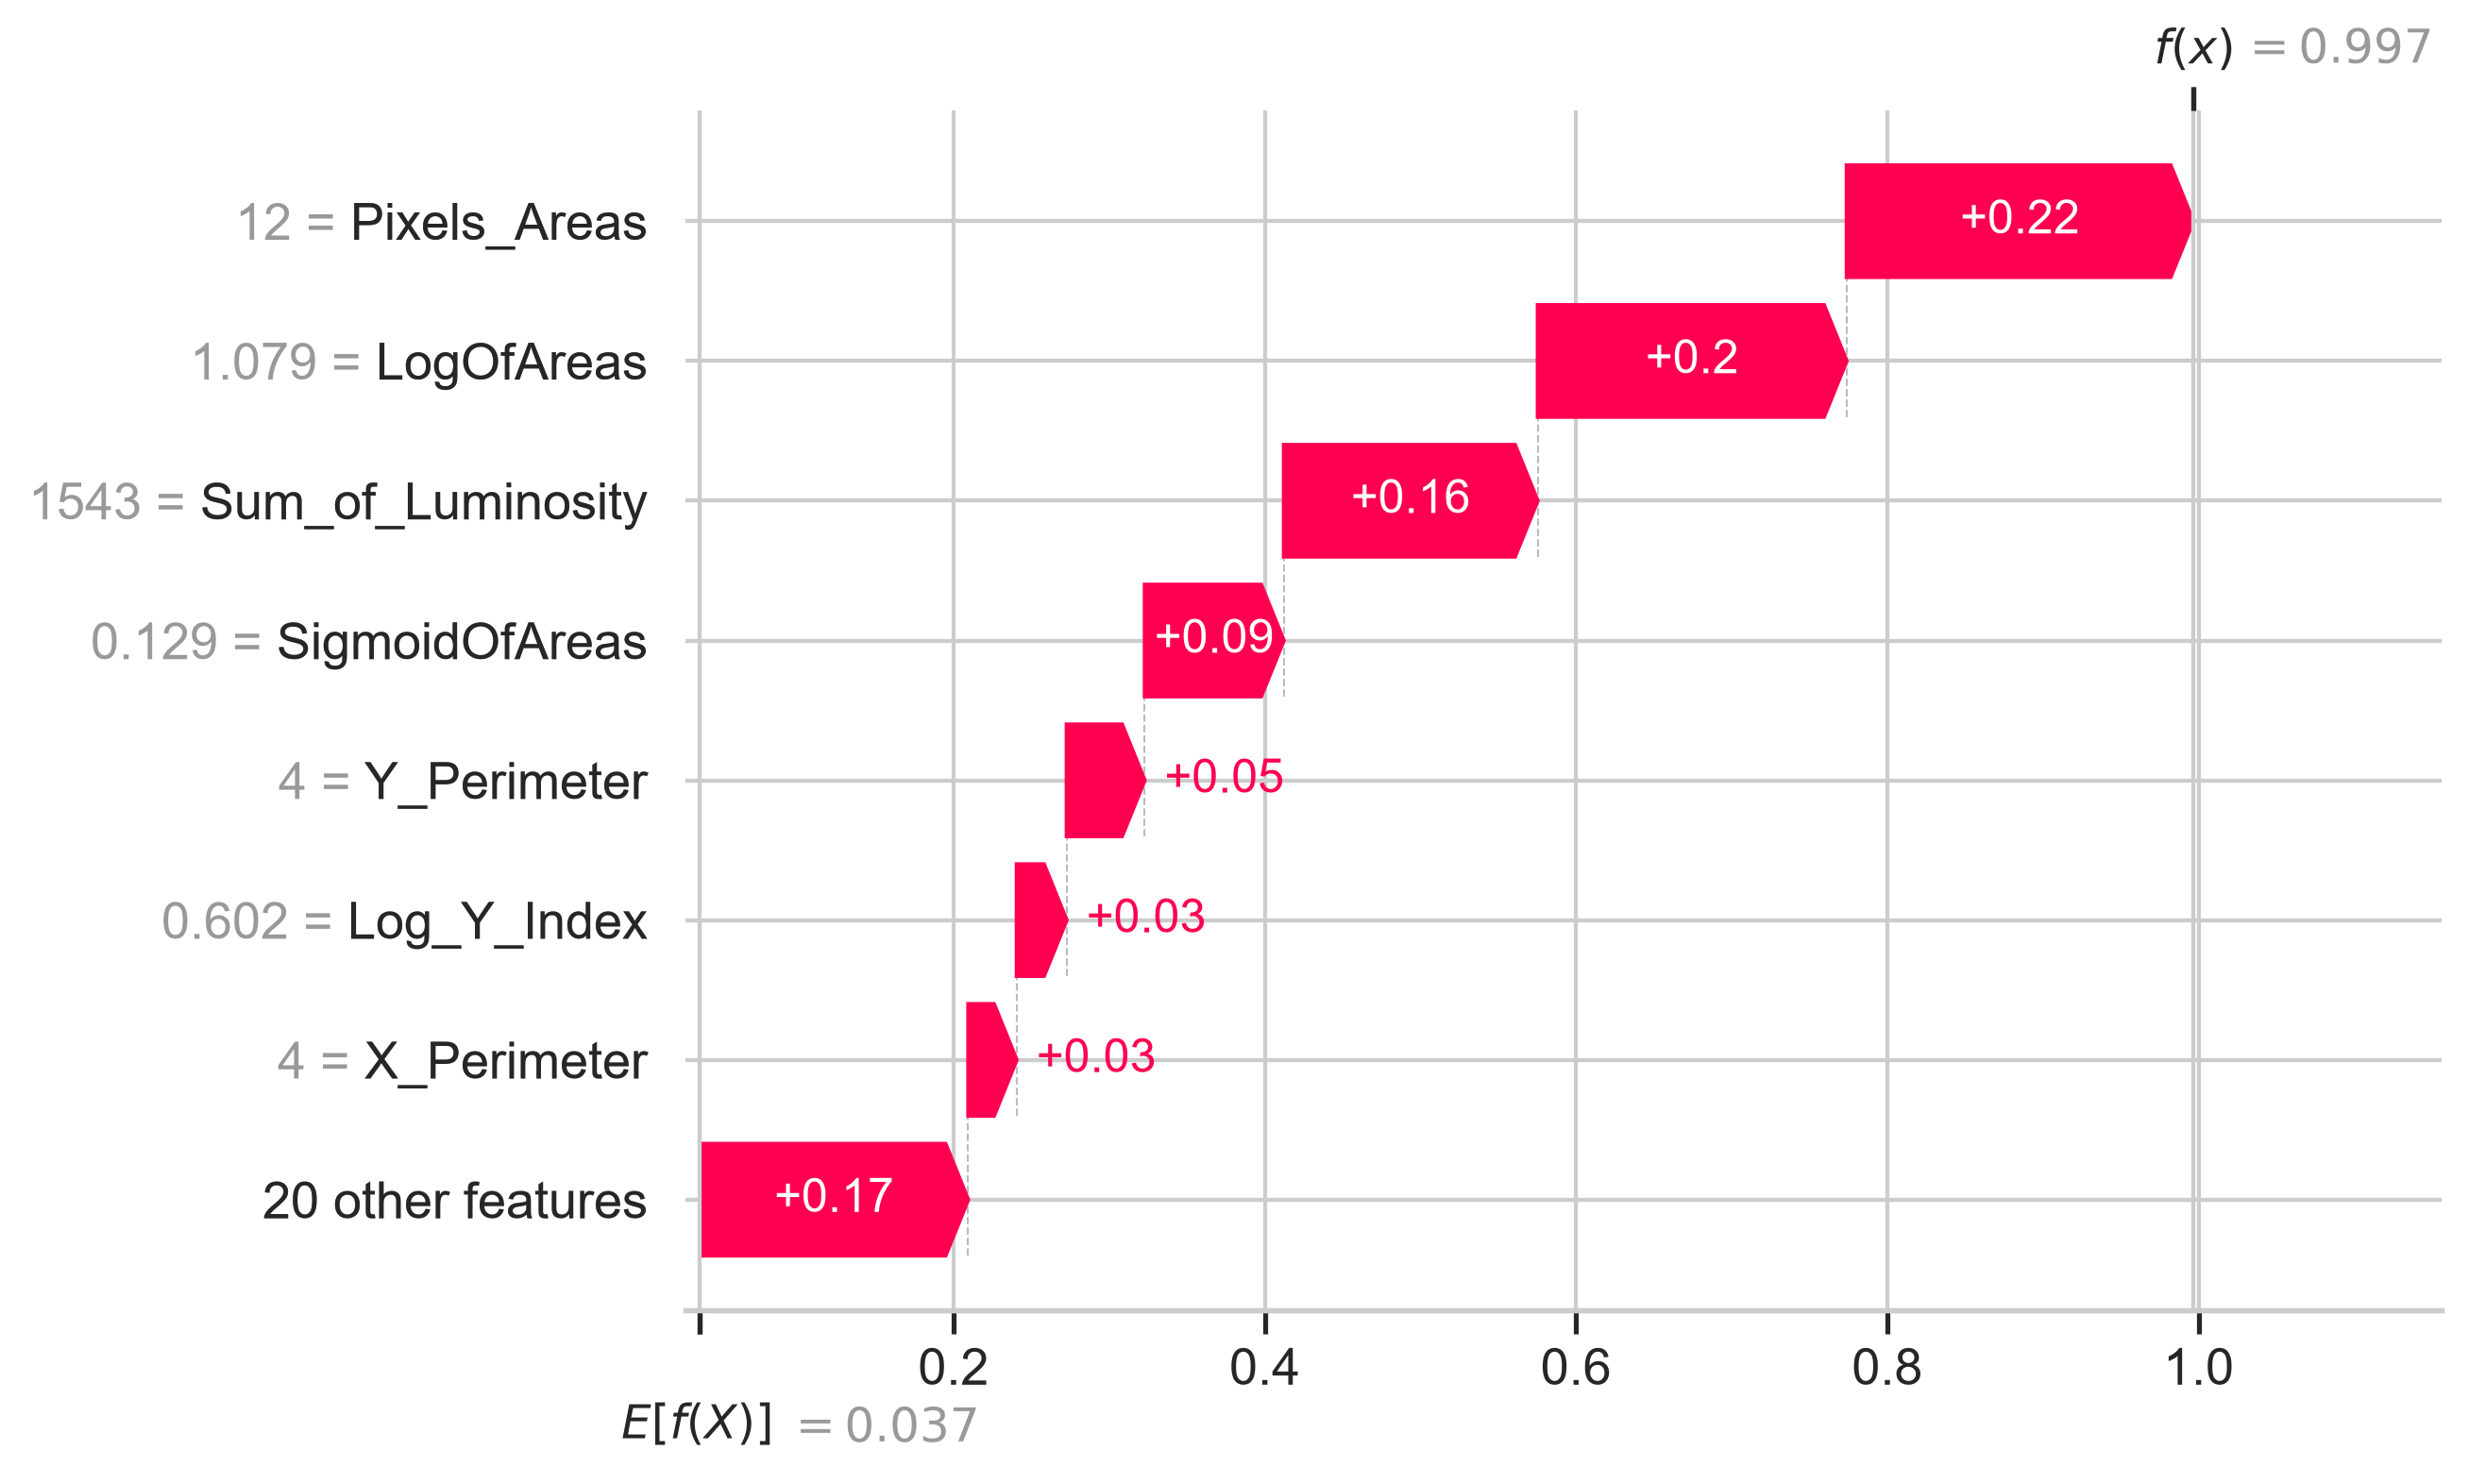
\includegraphics[keepaspectratio]{notebooks/08-ensembles_files/figure-pdf/cell-13-output-2.png}}

The waterfall plot starts at the average model output for this class and
adds the contribution of each feature until the prediction for this
plate is reached. A good explanation for a quality engineer names the
two or three largest contributions in physical terms, for example: ``The
model considers this a scratch mainly because the defect is long and
narrow and its luminosity is low -- typical for K\_Scatch.'' It should
also state what the explanation is \emph{not}: a causal statement about
the production process.

\end{tcolorbox}

\chapter{Unsupervised Learning and Anomaly
Detection}\label{unsupervised-learning-and-anomaly-detection}

In the previous chapters every training example came with a label: the
strength of the concrete, the failure of the machine, the type of
defect. In engineering, labels are often the scarcest resource. Failures
are rare, new fault types appear that nobody has seen before, and expert
labelling is slow and expensive. Yet we usually have plenty of data from
\textbf{normal operation}.

Unsupervised learning finds structure in data without labels. In this
chapter we use it for three purposes: to compress hundreds of correlated
sensor signals into a few meaningful components (PCA), to monitor a
process by detecting deviations from its normal behaviour, and to group
operating states or products into clusters.

\textbf{Scenario: an online alarm for the fab}

After the analysis in Chapter 2, the semiconductor fab decided to try an
unsupervised approach: a monitoring system that learns normal runs and
raises an alarm for unusual ones, without needing labelled failures.
Process engineering accepts an alarm only if it catches at least half of
the failed runs while raising false alarms on at most 5 \% of the good
runs -- otherwise operators will ignore it.

\textbf{Your decision:} Install the PCA-based alarm in the production
line?

\textbf{Learning goals.} After this chapter you can

\begin{itemize}
\tightlist
\item
  distinguish supervised and unsupervised learning and name engineering
  uses of the latter,
\item
  reduce high-dimensional process data with principal component analysis
  (PCA) and interpret scores, loadings and explained variance,
\item
  monitor a process with PCA-based statistics (Hotelling's T², SPE) and
  control limits,
\item
  group data with k-means and DBSCAN and choose the number of clusters,
\item
  detect anomalies with Isolation Forest and evaluate detectors when a
  few labels are available.
\end{itemize}

\textbf{Datasets in this chapter}

\begin{itemize}
\tightlist
\item
  \href{https://archive.ics.uci.edu/dataset/179/secom}{SECOM (UCI)}
\item
  \href{https://archive.ics.uci.edu/dataset/447/condition+monitoring+of+hydraulic+systems}{Condition
  Monitoring of Hydraulic Systems (UCI)}
\end{itemize}

\section{Principal component
analysis}\label{principal-component-analysis}

Process data are highly redundant: dozens of temperatures in the same
furnace, pressures along the same line, currents of coupled drives all
move together. PCA exploits this redundancy.

\begin{tcolorbox}[enhanced jigsaw, colframe=quarto-callout-note-color-frame, toprule=.15mm, rightrule=.15mm, title=\textcolor{quarto-callout-note-color}{\faInfo}\hspace{0.5em}{Definition: Principal component analysis (PCA)}, colbacktitle=quarto-callout-note-color!10!white, left=2mm, titlerule=0mm, bottomtitle=1mm, toptitle=1mm, opacityback=0, bottomrule=.15mm, breakable, arc=.35mm, opacitybacktitle=0.6, colback=white, coltitle=black, leftrule=.75mm]

Given standardised data \(Z \in \mathbb{R}^{n \times p}\) (each column
with mean 0 and standard deviation 1), PCA finds orthogonal directions
\(v_1, v_2, \dots\) (the \textbf{loadings}) such that the projection of
the data onto \(v_1\) has maximal variance, the projection onto \(v_2\)
has maximal variance among all directions orthogonal to \(v_1\), and so
on. The projections \(Z v_j\) of the data onto the loadings are the
\textbf{scores} of component \(j\). Computationally, PCA is the singular
value decomposition \[Z = U \Sigma V^\top,\] where the columns of \(V\)
are the loadings and the variance explained by component \(j\) is
proportional to the squared singular value \(\sigma_j^2\).

\end{tcolorbox}

Keeping the first \(k\) components gives the best possible approximation
of the data by a \(k\)-dimensional plane (in the least-squares sense).
The \textbf{scree plot} (explained variance per component) and the
cumulative explained variance help to choose \(k\).

\begin{tcolorbox}[enhanced jigsaw, colframe=quarto-callout-warning-color-frame, toprule=.15mm, rightrule=.15mm, title=\textcolor{quarto-callout-warning-color}{\faExclamationTriangle}\hspace{0.5em}{Pitfall: standardise before PCA}, colbacktitle=quarto-callout-warning-color!10!white, left=2mm, titlerule=0mm, bottomtitle=1mm, toptitle=1mm, opacityback=0, bottomrule=.15mm, breakable, arc=.35mm, opacitybacktitle=0.6, colback=white, coltitle=black, leftrule=.75mm]

PCA maximises variance, and variance depends on units. Without
standardisation, a pressure in Pa (values around \(10^5\)) dominates a
temperature in °C. Standardise unless all variables share a unit and
their natural variances are meaningful.

\end{tcolorbox}

\section{Process monitoring with PCA}\label{process-monitoring-with-pca}

The idea of multivariate statistical process control: build a PCA model
from data of \textbf{normal operation} (phase I) and then check every
new observation against it (phase II). Two complementary statistics
measure the deviation:

\begin{figure}[H]

\centering{

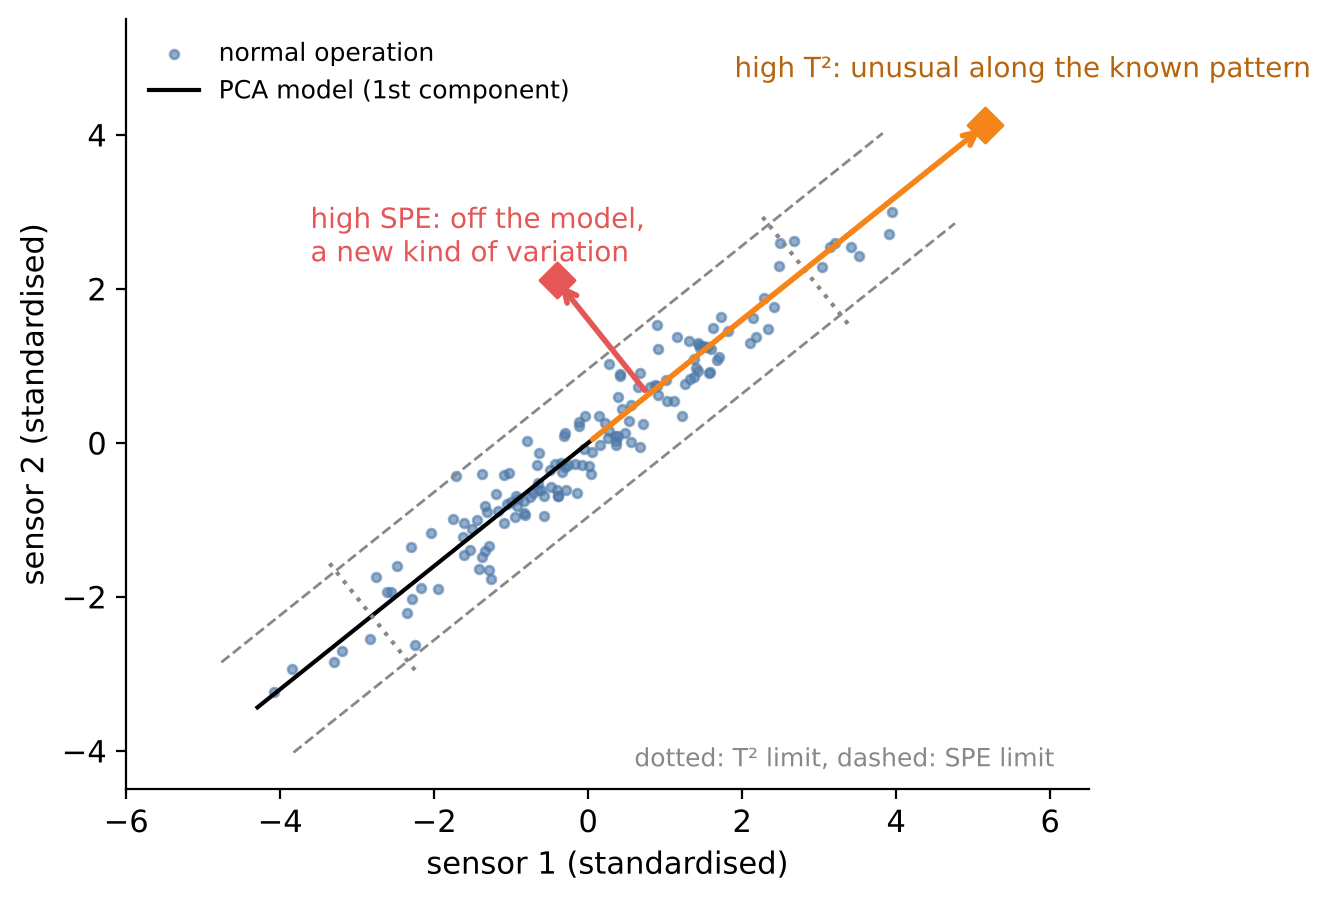
\includegraphics[width=0.75\linewidth,height=\textheight,keepaspectratio]{notebooks/images/pca-monitoring.png}

}

\caption{\label{fig-pcamon}Geometry of PCA monitoring, shown for two
correlated sensors and a one-component model (in practice: many sensors
and a model plane of several components). Hotelling's T² measures how
unusual an observation is \emph{within} the model (an extreme value
along the known pattern); the squared prediction error SPE measures its
distance \emph{from} the model (a new kind of variation the model has
never seen).}

\end{figure}%

\begin{tcolorbox}[enhanced jigsaw, colframe=quarto-callout-note-color-frame, toprule=.15mm, rightrule=.15mm, title=\textcolor{quarto-callout-note-color}{\faInfo}\hspace{0.5em}{Definition: Hotelling's T² and SPE}, colbacktitle=quarto-callout-note-color!10!white, left=2mm, titlerule=0mm, bottomtitle=1mm, toptitle=1mm, opacityback=0, bottomrule=.15mm, breakable, arc=.35mm, opacitybacktitle=0.6, colback=white, coltitle=black, leftrule=.75mm]

Let \(V_k = [v_1, \dots, v_k]\) contain the first \(k\) loadings and
\(\lambda_j\) be the variance of the scores of component \(j\) in the
normal-operation data. For a new standardised observation \(z\) with
scores \(t = V_k^\top z = (t_1, \dots, t_k)^\top\):
\[T^2 = \sum_{j=1}^k \frac{t_j^2}{\lambda_j}, \qquad \text{SPE} = \|z - V_k t\|^2 .\]
Control limits are derived from the normal-operation data, e.g.~as the
99 \% quantile of each statistic.

\end{tcolorbox}

When an alarm occurs, \textbf{contribution plots} show which original
variables contribute most to the large T² or SPE value -- a first hint
for the operator where to look.

\section{Clustering}\label{clustering}

Clustering groups observations so that members of a group are similar
and different groups are dissimilar. Engineering uses: identifying
operating modes of a machine (idle, part load, full load), grouping
products or customers, finding families of similar faults.

\begin{tcolorbox}[enhanced jigsaw, colframe=quarto-callout-note-color-frame, toprule=.15mm, rightrule=.15mm, title=\textcolor{quarto-callout-note-color}{\faInfo}\hspace{0.5em}{Definition: k-means}, colbacktitle=quarto-callout-note-color!10!white, left=2mm, titlerule=0mm, bottomtitle=1mm, toptitle=1mm, opacityback=0, bottomrule=.15mm, breakable, arc=.35mm, opacitybacktitle=0.6, colback=white, coltitle=black, leftrule=.75mm]

k-means partitions the data into \(k\) clusters by minimising the
within-cluster sum of squared distances to the cluster centres. The
algorithm alternates two steps until convergence: (1) assign each point
to the nearest centre, (2) move each centre to the mean of its points.
The result depends on the starting centres, so the algorithm is run
several times.

\end{tcolorbox}

k-means assumes roughly spherical clusters of similar size, and \(k\)
must be chosen: the \textbf{elbow} of the within-cluster sum of squares
or the \textbf{silhouette score} (how much closer a point is to its own
cluster than to the next one, between −1 and 1) help. \textbf{DBSCAN}
instead defines clusters as dense regions: it finds clusters of
arbitrary shape, determines their number itself and labels points in
sparse regions as noise -- a natural link to anomaly detection.

\section{Anomaly detection}\label{anomaly-detection}

\begin{tcolorbox}[enhanced jigsaw, colframe=quarto-callout-note-color-frame, toprule=.15mm, rightrule=.15mm, title=\textcolor{quarto-callout-note-color}{\faInfo}\hspace{0.5em}{Definition: Isolation Forest}, colbacktitle=quarto-callout-note-color!10!white, left=2mm, titlerule=0mm, bottomtitle=1mm, toptitle=1mm, opacityback=0, bottomrule=.15mm, breakable, arc=.35mm, opacitybacktitle=0.6, colback=white, coltitle=black, leftrule=.75mm]

An Isolation Forest builds random trees that split the data at random
features and random thresholds. Anomalies are ``few and different'':
they are isolated after few splits. The \textbf{anomaly score} is
derived from the average path length needed to isolate a point -- short
paths mean anomalous.

\end{tcolorbox}

\begin{tcolorbox}[enhanced jigsaw, colframe=quarto-callout-tip-color-frame, toprule=.15mm, rightrule=.15mm, title=\textcolor{quarto-callout-tip-color}{\faLightbulb}\hspace{0.5em}{Engineering practice: evaluating unsupervised detectors}, colbacktitle=quarto-callout-tip-color!10!white, left=2mm, titlerule=0mm, bottomtitle=1mm, toptitle=1mm, opacityback=0, bottomrule=.15mm, breakable, arc=.35mm, opacitybacktitle=0.6, colback=white, coltitle=black, leftrule=.75mm]

Even if the detector is trained without labels, a few labelled faults
are invaluable for \textbf{evaluating} it. Use them only for evaluation
and threshold selection, never for training -- and fit the model on
normal data that is separate from the normal data used for evaluation.

\end{tcolorbox}

\begin{Shaded}
\begin{Highlighting}[]
\CommentTok{\# Setup: works locally and in Google Colab}
\ImportTok{import}\NormalTok{ importlib.util, subprocess, sys}
\ControlFlowTok{for}\NormalTok{ pkg }\KeywordTok{in}\NormalTok{ [}\StringTok{"ucimlrepo"}\NormalTok{]:}
    \ControlFlowTok{if}\NormalTok{ importlib.util.find\_spec(pkg) }\KeywordTok{is} \VariableTok{None}\NormalTok{:}
\NormalTok{        subprocess.run([sys.executable, }\StringTok{"{-}m"}\NormalTok{, }\StringTok{"pip"}\NormalTok{, }\StringTok{"install"}\NormalTok{, }\StringTok{"{-}q"}\NormalTok{, pkg], check}\OperatorTok{=}\VariableTok{True}\NormalTok{)}

\ImportTok{import}\NormalTok{ numpy }\ImportTok{as}\NormalTok{ np}
\ImportTok{import}\NormalTok{ pandas }\ImportTok{as}\NormalTok{ pd}
\ImportTok{import}\NormalTok{ matplotlib.pyplot }\ImportTok{as}\NormalTok{ plt}
\ImportTok{import}\NormalTok{ seaborn }\ImportTok{as}\NormalTok{ sns}

\NormalTok{sns.set\_theme(style}\OperatorTok{=}\StringTok{"whitegrid"}\NormalTok{)}
\end{Highlighting}
\end{Shaded}

\section{Live coding: PCA monitoring of semiconductor
production}\label{live-coding-pca-monitoring-of-semiconductor-production}

We use the SECOM data introduced in Chapter 2: 1,567 production runs,
590 process measurements, and a pass/fail label. Following the
preparation from Chapter 2, we remove sparse and constant features,
impute the remaining gaps with the median and standardise. All
preprocessing steps and the PCA model are fitted on \textbf{passed runs
only} -- this is our model of normal operation.

\begin{Shaded}
\begin{Highlighting}[]
\ImportTok{from}\NormalTok{ ucimlrepo }\ImportTok{import}\NormalTok{ fetch\_ucirepo}
\ImportTok{from}\NormalTok{ sklearn.pipeline }\ImportTok{import}\NormalTok{ make\_pipeline}
\ImportTok{from}\NormalTok{ sklearn.impute }\ImportTok{import}\NormalTok{ SimpleImputer}
\ImportTok{from}\NormalTok{ sklearn.feature\_selection }\ImportTok{import}\NormalTok{ VarianceThreshold}
\ImportTok{from}\NormalTok{ sklearn.preprocessing }\ImportTok{import}\NormalTok{ StandardScaler}
\ImportTok{from}\NormalTok{ sklearn.decomposition }\ImportTok{import}\NormalTok{ PCA}

\KeywordTok{def}\NormalTok{ load\_secom():}
    \CommentTok{"""SECOM: return the process measurements X and the label y ({-}1 = pass, 1 = fail).}

\CommentTok{    In the UCI repository the label is not marked as target variable, so we find it}
\CommentTok{    ourselves: the only numeric column whose values are exactly {-}1 and 1.}
\CommentTok{    """}
\NormalTok{    df }\OperatorTok{=}\NormalTok{ fetch\_ucirepo(}\BuiltInTok{id}\OperatorTok{=}\DecValTok{179}\NormalTok{).data.original}
\NormalTok{    num }\OperatorTok{=}\NormalTok{ df.select\_dtypes(}\StringTok{"number"}\NormalTok{)}
\NormalTok{    labels }\OperatorTok{=}\NormalTok{ [c }\ControlFlowTok{for}\NormalTok{ c }\KeywordTok{in}\NormalTok{ num.columns }\ControlFlowTok{if} \BuiltInTok{set}\NormalTok{(num[c].dropna().unique()) }\OperatorTok{==}\NormalTok{ \{}\OperatorTok{{-}}\DecValTok{1}\NormalTok{, }\DecValTok{1}\NormalTok{\}]}
    \ControlFlowTok{if} \BuiltInTok{len}\NormalTok{(labels) }\OperatorTok{!=} \DecValTok{1}\NormalTok{:}
\NormalTok{        labels }\OperatorTok{=}\NormalTok{ [c }\ControlFlowTok{for}\NormalTok{ c }\KeywordTok{in}\NormalTok{ df.columns }\ControlFlowTok{if} \BuiltInTok{any}\NormalTok{(k }\KeywordTok{in} \BuiltInTok{str}\NormalTok{(c).lower() }\ControlFlowTok{for}\NormalTok{ k }\KeywordTok{in}\NormalTok{ (}\StringTok{"pass"}\NormalTok{, }\StringTok{"fail"}\NormalTok{, }\StringTok{"label"}\NormalTok{))]}
    \ControlFlowTok{assert} \BuiltInTok{len}\NormalTok{(labels) }\OperatorTok{==} \DecValTok{1}\NormalTok{, }\SpecialStringTok{f"Label column not found unambiguously: }\SpecialCharTok{\{}\NormalTok{labels}\SpecialCharTok{\}}\SpecialStringTok{"}
\NormalTok{    y }\OperatorTok{=}\NormalTok{ df[labels[}\DecValTok{0}\NormalTok{]].astype(}\BuiltInTok{int}\NormalTok{)}
\NormalTok{    X }\OperatorTok{=}\NormalTok{ num.drop(columns}\OperatorTok{=}\NormalTok{labels, errors}\OperatorTok{=}\StringTok{"ignore"}\NormalTok{)}
    \BuiltInTok{print}\NormalTok{(}\SpecialStringTok{f"Label column: }\SpecialCharTok{\{}\NormalTok{labels[}\DecValTok{0}\NormalTok{]}\SpecialCharTok{!r\}}\SpecialStringTok{, measurement columns: }\SpecialCharTok{\{}\NormalTok{X}\SpecialCharTok{.}\NormalTok{shape[}\DecValTok{1}\NormalTok{]}\SpecialCharTok{\}}\SpecialStringTok{, "}
          \SpecialStringTok{f"ignored non{-}numeric columns: }\SpecialCharTok{\{}\NormalTok{[c }\ControlFlowTok{for}\NormalTok{ c }\KeywordTok{in}\NormalTok{ df.columns }\ControlFlowTok{if}\NormalTok{ c }\KeywordTok{not} \KeywordTok{in}\NormalTok{ num.columns]}\SpecialCharTok{\}}\SpecialStringTok{"}\NormalTok{)}
    \ControlFlowTok{return}\NormalTok{ X, y}

\NormalTok{X, y }\OperatorTok{=}\NormalTok{ load\_secom()                          }\CommentTok{\# helper from Chapter 2}
\NormalTok{X }\OperatorTok{=}\NormalTok{ X.loc[:, X.isna().mean() }\OperatorTok{\textless{}} \FloatTok{0.5}\NormalTok{]          }\CommentTok{\# drop features with \textgreater{} 50 \% missing}

\NormalTok{prep }\OperatorTok{=}\NormalTok{ make\_pipeline(SimpleImputer(strategy}\OperatorTok{=}\StringTok{"median"}\NormalTok{), VarianceThreshold(}\FloatTok{1e{-}8}\NormalTok{), StandardScaler())}
\NormalTok{Z }\OperatorTok{=}\NormalTok{ prep.fit\_transform(X[y }\OperatorTok{==} \OperatorTok{{-}}\DecValTok{1}\NormalTok{])           }\CommentTok{\# model of normal operation}
\NormalTok{pca }\OperatorTok{=}\NormalTok{ PCA().fit(Z)}
\NormalTok{cum }\OperatorTok{=}\NormalTok{ np.cumsum(pca.explained\_variance\_ratio\_)}
\NormalTok{k }\OperatorTok{=} \BuiltInTok{int}\NormalTok{(np.searchsorted(cum, }\FloatTok{0.80}\NormalTok{) }\OperatorTok{+} \DecValTok{1}\NormalTok{)}
\NormalTok{plt.plot(np.arange(}\DecValTok{1}\NormalTok{, }\DecValTok{101}\NormalTok{), cum[:}\DecValTok{100}\NormalTok{])}\OperatorTok{;}\NormalTok{ plt.axhline(}\FloatTok{0.8}\NormalTok{, ls}\OperatorTok{=}\StringTok{"{-}{-}"}\NormalTok{, c}\OperatorTok{=}\StringTok{"k"}\NormalTok{)}
\NormalTok{plt.xlabel(}\StringTok{"Number of components"}\NormalTok{)}\OperatorTok{;}\NormalTok{ plt.ylabel(}\StringTok{"Cumulative explained variance"}\NormalTok{)}
\NormalTok{plt.show()}
\BuiltInTok{print}\NormalTok{(}\StringTok{"Components for 80 \% variance:"}\NormalTok{, k)}
\end{Highlighting}
\end{Shaded}

\begin{verbatim}
Label column: 'class', measurement columns: 590, ignored non-numeric columns: ['timestamp']
\end{verbatim}

\pandocbounded{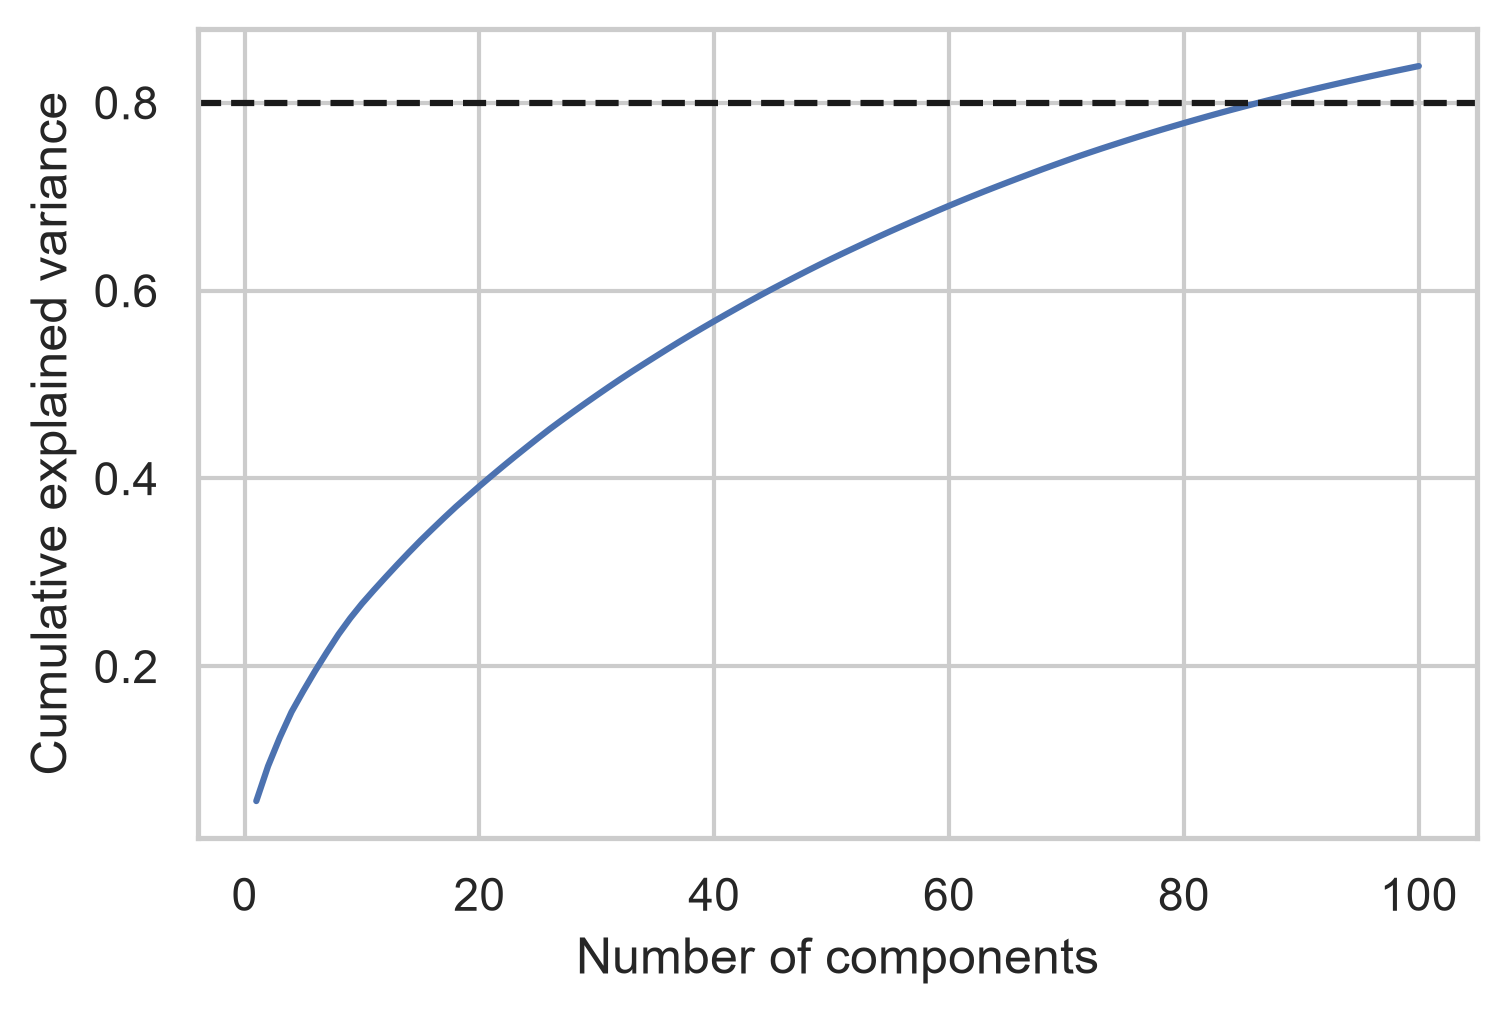
\includegraphics[keepaspectratio]{notebooks/09-unsupervised_files/figure-pdf/cell-3-output-2.png}}

\begin{verbatim}
Components for 80 % variance: 87
\end{verbatim}

\textbf{Discussion.} The cumulative explained variance rises steeply for
the first components and then slowly. For SECOM, many components are
needed to reach 80 \% -- the process has many partly independent sources
of variation, and much of the variance is noise. The choice of 80 \% is
a convention; in monitoring, the number of components is often chosen by
cross-validation of the reconstruction error or by the scree plot's
elbow.

\begin{Shaded}
\begin{Highlighting}[]
\NormalTok{pca\_k }\OperatorTok{=}\NormalTok{ PCA(k).fit(Z)}

\KeywordTok{def}\NormalTok{ t2\_spe(Zx):}
\NormalTok{    scores }\OperatorTok{=}\NormalTok{ pca\_k.transform(Zx)}
\NormalTok{    t2 }\OperatorTok{=}\NormalTok{ np.}\BuiltInTok{sum}\NormalTok{(scores}\OperatorTok{**}\DecValTok{2} \OperatorTok{/}\NormalTok{ pca\_k.explained\_variance\_, axis}\OperatorTok{=}\DecValTok{1}\NormalTok{)}
\NormalTok{    spe }\OperatorTok{=}\NormalTok{ np.}\BuiltInTok{sum}\NormalTok{((Zx }\OperatorTok{{-}}\NormalTok{ pca\_k.inverse\_transform(scores))}\OperatorTok{**}\DecValTok{2}\NormalTok{, axis}\OperatorTok{=}\DecValTok{1}\NormalTok{)}
    \ControlFlowTok{return}\NormalTok{ t2, spe}

\NormalTok{t2, spe }\OperatorTok{=}\NormalTok{ t2\_spe(prep.transform(X))}
\NormalTok{t2\_lim, spe\_lim }\OperatorTok{=}\NormalTok{ np.percentile(t2[y }\OperatorTok{==} \OperatorTok{{-}}\DecValTok{1}\NormalTok{], }\DecValTok{99}\NormalTok{), np.percentile(spe[y }\OperatorTok{==} \OperatorTok{{-}}\DecValTok{1}\NormalTok{], }\DecValTok{99}\NormalTok{)}

\NormalTok{plt.scatter(t2, spe, c}\OperatorTok{=}\NormalTok{(y }\OperatorTok{==} \DecValTok{1}\NormalTok{), cmap}\OperatorTok{=}\StringTok{"coolwarm"}\NormalTok{, s}\OperatorTok{=}\DecValTok{8}\NormalTok{, alpha}\OperatorTok{=}\FloatTok{0.6}\NormalTok{)}
\NormalTok{plt.axvline(t2\_lim, c}\OperatorTok{=}\StringTok{"k"}\NormalTok{, ls}\OperatorTok{=}\StringTok{"{-}{-}"}\NormalTok{)}\OperatorTok{;}\NormalTok{ plt.axhline(spe\_lim, c}\OperatorTok{=}\StringTok{"k"}\NormalTok{, ls}\OperatorTok{=}\StringTok{"{-}{-}"}\NormalTok{)}
\NormalTok{plt.xscale(}\StringTok{"log"}\NormalTok{)}\OperatorTok{;}\NormalTok{ plt.yscale(}\StringTok{"log"}\NormalTok{)}\OperatorTok{;}\NormalTok{ plt.xlabel(}\StringTok{"Hotelling T²"}\NormalTok{)}\OperatorTok{;}\NormalTok{ plt.ylabel(}\StringTok{"SPE"}\NormalTok{)}
\NormalTok{plt.title(}\StringTok{"Red: failed runs, dashed: 99 }\SpecialCharTok{\% li}\StringTok{mits of normal runs"}\NormalTok{)}
\NormalTok{plt.show()}
\end{Highlighting}
\end{Shaded}

\pandocbounded{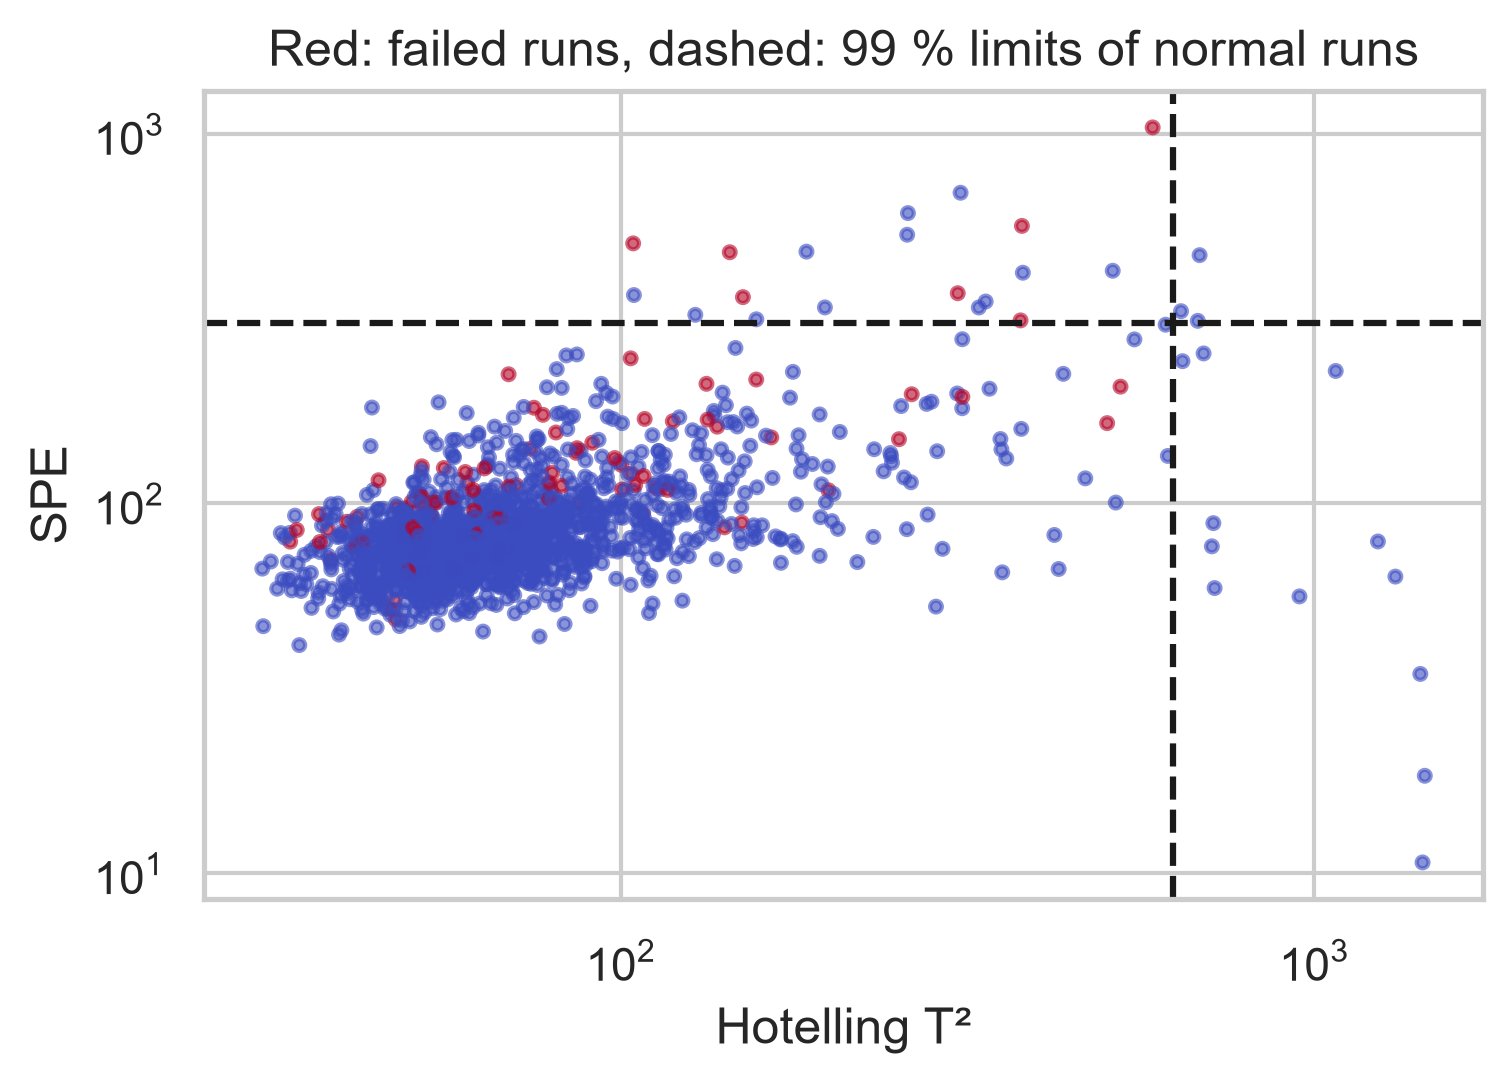
\includegraphics[keepaspectratio]{notebooks/09-unsupervised_files/figure-pdf/cell-4-output-1.png}}

\textbf{Discussion.} The dashed lines are the 99 \% limits of the normal
runs, so about 1 \% of normal runs exceed each limit by construction
(false alarms). Failed runs that exceed a limit are detected; those
inside the limits look normal to the model. If most failures lie inside
the limits, the measured variables may not contain the cause of the
failure, or the failure manifests itself in variables that were removed,
or in a way that PCA does not capture.

\begin{Shaded}
\begin{Highlighting}[]
\ImportTok{from}\NormalTok{ sklearn.ensemble }\ImportTok{import}\NormalTok{ IsolationForest}
\ImportTok{from}\NormalTok{ sklearn.metrics }\ImportTok{import}\NormalTok{ roc\_auc\_score}

\NormalTok{iso }\OperatorTok{=}\NormalTok{ IsolationForest(n\_estimators}\OperatorTok{=}\DecValTok{300}\NormalTok{, random\_state}\OperatorTok{=}\DecValTok{0}\NormalTok{).fit(Z)}
\NormalTok{score }\OperatorTok{=} \OperatorTok{{-}}\NormalTok{iso.score\_samples(prep.transform(X))}
\BuiltInTok{print}\NormalTok{(}\SpecialStringTok{f"ROC AUC  Isolation Forest: }\SpecialCharTok{\{}\NormalTok{roc\_auc\_score(y }\OperatorTok{==} \DecValTok{1}\NormalTok{, score)}\SpecialCharTok{:.3f\}}\SpecialStringTok{"}\NormalTok{)}
\BuiltInTok{print}\NormalTok{(}\SpecialStringTok{f"ROC AUC  T²:               }\SpecialCharTok{\{}\NormalTok{roc\_auc\_score(y }\OperatorTok{==} \DecValTok{1}\NormalTok{, t2)}\SpecialCharTok{:.3f\}}\SpecialStringTok{"}\NormalTok{)}
\BuiltInTok{print}\NormalTok{(}\SpecialStringTok{f"ROC AUC  SPE:              }\SpecialCharTok{\{}\NormalTok{roc\_auc\_score(y }\OperatorTok{==} \DecValTok{1}\NormalTok{, spe)}\SpecialCharTok{:.3f\}}\SpecialStringTok{"}\NormalTok{)}
\end{Highlighting}
\end{Shaded}

\begin{verbatim}
ROC AUC  Isolation Forest: 0.571
ROC AUC  T²:               0.528
ROC AUC  SPE:              0.741
\end{verbatim}

\begin{tcolorbox}[enhanced jigsaw, colframe=quarto-callout-warning-color-frame, toprule=.15mm, rightrule=.15mm, title=\textcolor{quarto-callout-warning-color}{\faExclamationTriangle}\hspace{0.5em}{Pitfall: evaluating on the training data}, colbacktitle=quarto-callout-warning-color!10!white, left=2mm, titlerule=0mm, bottomtitle=1mm, toptitle=1mm, opacityback=0, bottomrule=.15mm, breakable, arc=.35mm, opacitybacktitle=0.6, colback=white, coltitle=black, leftrule=.75mm]

In this quick comparison, the normal runs used to fit the models are
also part of the evaluation. They naturally look ``very normal'' to the
models, which makes the result optimistic. Exercise 1 repeats the
evaluation properly with separate normal runs.

\end{tcolorbox}

For SECOM, expect modest AUC values: fault detection in semiconductor
manufacturing from summary process data is known to be hard. This is a
realistic lesson -- many sensors do not guarantee that the relevant
information is in the data.

\section{Back to the decision}\label{back-to-the-decision-8}

The requirement fixes the false alarm rate at 5 \%, so we set the alarm
limit at the 95 \% quantile of the statistic on \emph{good} runs and
then measure which share of the failed runs exceeds it. To avoid the
optimism discussed above, we fit preprocessing and PCA on 70 \% of the
good runs and evaluate on the remaining good runs plus all failed runs.

\begin{Shaded}
\begin{Highlighting}[]
\ImportTok{from}\NormalTok{ sklearn.model\_selection }\ImportTok{import}\NormalTok{ train\_test\_split}

\NormalTok{X\_good\_fit, X\_good\_eval }\OperatorTok{=}\NormalTok{ train\_test\_split(X[y }\OperatorTok{==} \OperatorTok{{-}}\DecValTok{1}\NormalTok{], test\_size}\OperatorTok{=}\FloatTok{0.3}\NormalTok{, random\_state}\OperatorTok{=}\DecValTok{0}\NormalTok{)}
\NormalTok{prep\_d }\OperatorTok{=}\NormalTok{ make\_pipeline(SimpleImputer(strategy}\OperatorTok{=}\StringTok{"median"}\NormalTok{), VarianceThreshold(}\FloatTok{1e{-}8}\NormalTok{), StandardScaler())}
\NormalTok{Z\_fit }\OperatorTok{=}\NormalTok{ prep\_d.fit\_transform(X\_good\_fit)}
\NormalTok{pca\_d }\OperatorTok{=}\NormalTok{ PCA(k).fit(Z\_fit)}

\KeywordTok{def}\NormalTok{ spe\_of(Zx):}
    \ControlFlowTok{return}\NormalTok{ np.}\BuiltInTok{sum}\NormalTok{((Zx }\OperatorTok{{-}}\NormalTok{ pca\_d.inverse\_transform(pca\_d.transform(Zx)))}\OperatorTok{**}\DecValTok{2}\NormalTok{, axis}\OperatorTok{=}\DecValTok{1}\NormalTok{)}

\NormalTok{limit }\OperatorTok{=}\NormalTok{ np.percentile(spe\_of(prep\_d.transform(X\_good\_eval)), }\DecValTok{95}\NormalTok{)}
\NormalTok{detection }\OperatorTok{=}\NormalTok{ (spe\_of(prep\_d.transform(X[y }\OperatorTok{==} \DecValTok{1}\NormalTok{])) }\OperatorTok{\textgreater{}}\NormalTok{ limit).mean()}
\BuiltInTok{print}\NormalTok{(}\SpecialStringTok{f"False alarm rate on good runs: 5 \% (by construction), detection rate of failed runs: }\SpecialCharTok{\{}\NormalTok{detection}\SpecialCharTok{:.0\%\}}\SpecialStringTok{"}\NormalTok{)}
\BuiltInTok{print}\NormalTok{(}\StringTok{"Decision:"}\NormalTok{, }\StringTok{"install the alarm."} \ControlFlowTok{if}\NormalTok{ detection }\OperatorTok{\textgreater{}=} \FloatTok{0.5} \ControlFlowTok{else} \StringTok{"do not install – the alarm would miss too many failures."}\NormalTok{)}
\end{Highlighting}
\end{Shaded}

\begin{verbatim}
False alarm rate on good runs: 5 % (by construction), detection rate of failed runs: 11%
Decision: do not install – the alarm would miss too many failures.
\end{verbatim}

(Strictly, the limit should be set on one part of the held-out good runs
and the false alarm rate checked on another; with a few hundred good
runs we accept this simplification.) If the detection rate falls short,
the result is still valuable: it tells the fab that the summary data do
not contain enough information about the failures -- and that investing
in different measurements is more promising than tuning the algorithm.

\section{Live coding: operating states of a hydraulic test
rig}\label{live-coding-operating-states-of-a-hydraulic-test-rig}

The hydraulic dataset was recorded on a test rig in which the condition
of four components -- cooler, valve, pump and accumulator -- was varied
deliberately. Each of the 2,205 load cycles lasts 60 seconds; 17 sensors
were recorded at up to 100 Hz. The file \texttt{profile.txt} contains
the component conditions, e.g.~the cooler efficiency (3 \%, 20 \% or 100
\%). We compute simple features per cycle from the temperature sensors
and the cooling efficiency and see whether PCA and k-means recover the
cooler condition \textbf{without} using the labels.

\begin{Shaded}
\begin{Highlighting}[]
\ImportTok{import}\NormalTok{ zipfile, io, requests}
\ImportTok{from}\NormalTok{ pathlib }\ImportTok{import}\NormalTok{ Path}

\NormalTok{DATA }\OperatorTok{=}\NormalTok{ Path(}\StringTok{"data"}\NormalTok{)}\OperatorTok{;}\NormalTok{ DATA.mkdir(exist\_ok}\OperatorTok{=}\VariableTok{True}\NormalTok{)}
\NormalTok{hz }\OperatorTok{=}\NormalTok{ DATA }\OperatorTok{/} \StringTok{"hydraulic.zip"}
\ControlFlowTok{if} \KeywordTok{not}\NormalTok{ hz.exists():}
\NormalTok{    hz.write\_bytes(requests.get(}\StringTok{"https://archive.ics.uci.edu/static/public/447/"}
                                \StringTok{"condition+monitoring+of+hydraulic+systems.zip"}\NormalTok{, timeout}\OperatorTok{=}\DecValTok{300}\NormalTok{).content)}

\KeywordTok{def}\NormalTok{ read\_sensor(z, name):}
\NormalTok{    member }\OperatorTok{=} \BuiltInTok{next}\NormalTok{(n }\ControlFlowTok{for}\NormalTok{ n }\KeywordTok{in}\NormalTok{ z.namelist() }\ControlFlowTok{if}\NormalTok{ n.endswith(name))}
    \ControlFlowTok{return}\NormalTok{ pd.read\_csv(z.}\BuiltInTok{open}\NormalTok{(member), sep}\OperatorTok{=}\StringTok{"}\CharTok{\textbackslash{}t}\StringTok{"}\NormalTok{, header}\OperatorTok{=}\VariableTok{None}\NormalTok{).values}

\ControlFlowTok{with}\NormalTok{ zipfile.ZipFile(hz) }\ImportTok{as}\NormalTok{ z:}
\NormalTok{    sensors }\OperatorTok{=}\NormalTok{ \{s: read\_sensor(z, }\SpecialStringTok{f"}\SpecialCharTok{\{}\NormalTok{s}\SpecialCharTok{\}}\SpecialStringTok{.txt"}\NormalTok{) }\ControlFlowTok{for}\NormalTok{ s }\KeywordTok{in}\NormalTok{ [}\StringTok{"TS1"}\NormalTok{, }\StringTok{"TS2"}\NormalTok{, }\StringTok{"TS3"}\NormalTok{, }\StringTok{"TS4"}\NormalTok{, }\StringTok{"CE"}\NormalTok{, }\StringTok{"CP"}\NormalTok{]\}}
\NormalTok{    profile }\OperatorTok{=}\NormalTok{ pd.DataFrame(read\_sensor(z, }\StringTok{"profile.txt"}\NormalTok{),}
\NormalTok{                           columns}\OperatorTok{=}\NormalTok{[}\StringTok{"cooler"}\NormalTok{, }\StringTok{"valve"}\NormalTok{, }\StringTok{"pump\_leak"}\NormalTok{, }\StringTok{"accumulator"}\NormalTok{, }\StringTok{"stable"}\NormalTok{])}

\NormalTok{feat }\OperatorTok{=}\NormalTok{ pd.DataFrame(\{}\SpecialStringTok{f"}\SpecialCharTok{\{}\NormalTok{s}\SpecialCharTok{\}}\SpecialStringTok{\_}\SpecialCharTok{\{}\NormalTok{stat}\SpecialCharTok{\}}\SpecialStringTok{"}\NormalTok{: }\BuiltInTok{getattr}\NormalTok{(np, stat)(v, axis}\OperatorTok{=}\DecValTok{1}\NormalTok{)}
                     \ControlFlowTok{for}\NormalTok{ s, v }\KeywordTok{in}\NormalTok{ sensors.items() }\ControlFlowTok{for}\NormalTok{ stat }\KeywordTok{in}\NormalTok{ [}\StringTok{"mean"}\NormalTok{, }\StringTok{"std"}\NormalTok{]\})}
\NormalTok{feat.shape}
\end{Highlighting}
\end{Shaded}

\begin{verbatim}
(2205, 12)
\end{verbatim}

\begin{Shaded}
\begin{Highlighting}[]
\ImportTok{from}\NormalTok{ sklearn.cluster }\ImportTok{import}\NormalTok{ KMeans}
\ImportTok{from}\NormalTok{ sklearn.metrics }\ImportTok{import}\NormalTok{ silhouette\_score}

\NormalTok{Zh }\OperatorTok{=}\NormalTok{ StandardScaler().fit\_transform(feat)}
\NormalTok{scores\_h }\OperatorTok{=}\NormalTok{ PCA(}\DecValTok{2}\NormalTok{).fit\_transform(Zh)}

\NormalTok{sil }\OperatorTok{=}\NormalTok{ \{k\_: silhouette\_score(Zh, KMeans(k\_, n\_init}\OperatorTok{=}\DecValTok{10}\NormalTok{, random\_state}\OperatorTok{=}\DecValTok{0}\NormalTok{).fit\_predict(Zh)) }\ControlFlowTok{for}\NormalTok{ k\_ }\KeywordTok{in} \BuiltInTok{range}\NormalTok{(}\DecValTok{2}\NormalTok{, }\DecValTok{7}\NormalTok{)\}}
\BuiltInTok{print}\NormalTok{(}\StringTok{"Silhouette scores:"}\NormalTok{, \{k\_: }\BuiltInTok{round}\NormalTok{(v, }\DecValTok{3}\NormalTok{) }\ControlFlowTok{for}\NormalTok{ k\_, v }\KeywordTok{in}\NormalTok{ sil.items()\})}
\NormalTok{clusters }\OperatorTok{=}\NormalTok{ KMeans(}\DecValTok{3}\NormalTok{, n\_init}\OperatorTok{=}\DecValTok{10}\NormalTok{, random\_state}\OperatorTok{=}\DecValTok{0}\NormalTok{).fit\_predict(Zh)}

\NormalTok{fig, axes }\OperatorTok{=}\NormalTok{ plt.subplots(}\DecValTok{1}\NormalTok{, }\DecValTok{2}\NormalTok{, figsize}\OperatorTok{=}\NormalTok{(}\DecValTok{12}\NormalTok{, }\FloatTok{4.5}\NormalTok{))}
\NormalTok{sns.scatterplot(x}\OperatorTok{=}\NormalTok{scores\_h[:, }\DecValTok{0}\NormalTok{], y}\OperatorTok{=}\NormalTok{scores\_h[:, }\DecValTok{1}\NormalTok{], hue}\OperatorTok{=}\NormalTok{profile[}\StringTok{"cooler"}\NormalTok{].astype(}\BuiltInTok{int}\NormalTok{).astype(}\BuiltInTok{str}\NormalTok{),}
\NormalTok{                ax}\OperatorTok{=}\NormalTok{axes[}\DecValTok{0}\NormalTok{], s}\OperatorTok{=}\DecValTok{12}\NormalTok{).}\BuiltInTok{set}\NormalTok{(title}\OperatorTok{=}\StringTok{"Coloured by true cooler condition (\%)"}\NormalTok{, xlabel}\OperatorTok{=}\StringTok{"PC 1"}\NormalTok{, ylabel}\OperatorTok{=}\StringTok{"PC 2"}\NormalTok{)}
\NormalTok{sns.scatterplot(x}\OperatorTok{=}\NormalTok{scores\_h[:, }\DecValTok{0}\NormalTok{], y}\OperatorTok{=}\NormalTok{scores\_h[:, }\DecValTok{1}\NormalTok{], hue}\OperatorTok{=}\NormalTok{clusters.astype(}\BuiltInTok{str}\NormalTok{), ax}\OperatorTok{=}\NormalTok{axes[}\DecValTok{1}\NormalTok{], s}\OperatorTok{=}\DecValTok{12}\NormalTok{,}
\NormalTok{                palette}\OperatorTok{=}\StringTok{"Set2"}\NormalTok{).}\BuiltInTok{set}\NormalTok{(title}\OperatorTok{=}\StringTok{"Coloured by k{-}means cluster"}\NormalTok{, xlabel}\OperatorTok{=}\StringTok{"PC 1"}\NormalTok{, ylabel}\OperatorTok{=}\StringTok{"PC 2"}\NormalTok{)}
\NormalTok{plt.tight\_layout()}\OperatorTok{;}\NormalTok{ plt.show()}
\NormalTok{pd.crosstab(profile[}\StringTok{"cooler"}\NormalTok{], clusters, rownames}\OperatorTok{=}\NormalTok{[}\StringTok{"cooler \%"}\NormalTok{], colnames}\OperatorTok{=}\NormalTok{[}\StringTok{"cluster"}\NormalTok{])}
\end{Highlighting}
\end{Shaded}

\begin{verbatim}
C:\Tools\Anaconda\Lib\site-packages\sklearn\cluster\_kmeans.py:1424: UserWarning: KMeans is known to have a memory leak on Windows with MKL, when there are less chunks than available threads. You can avoid it by setting the environment variable OMP_NUM_THREADS=9.
  warnings.warn(
C:\Tools\Anaconda\Lib\site-packages\sklearn\cluster\_kmeans.py:1424: UserWarning: KMeans is known to have a memory leak on Windows with MKL, when there are less chunks than available threads. You can avoid it by setting the environment variable OMP_NUM_THREADS=9.
  warnings.warn(
C:\Tools\Anaconda\Lib\site-packages\sklearn\cluster\_kmeans.py:1424: UserWarning: KMeans is known to have a memory leak on Windows with MKL, when there are less chunks than available threads. You can avoid it by setting the environment variable OMP_NUM_THREADS=9.
  warnings.warn(
C:\Tools\Anaconda\Lib\site-packages\sklearn\cluster\_kmeans.py:1424: UserWarning: KMeans is known to have a memory leak on Windows with MKL, when there are less chunks than available threads. You can avoid it by setting the environment variable OMP_NUM_THREADS=9.
  warnings.warn(
C:\Tools\Anaconda\Lib\site-packages\sklearn\cluster\_kmeans.py:1424: UserWarning: KMeans is known to have a memory leak on Windows with MKL, when there are less chunks than available threads. You can avoid it by setting the environment variable OMP_NUM_THREADS=9.
  warnings.warn(
\end{verbatim}

\begin{verbatim}
Silhouette scores: {2: 0.543, 3: 0.551, 4: 0.542, 5: 0.558, 6: 0.563}
\end{verbatim}

\begin{verbatim}
C:\Tools\Anaconda\Lib\site-packages\sklearn\cluster\_kmeans.py:1424: UserWarning: KMeans is known to have a memory leak on Windows with MKL, when there are less chunks than available threads. You can avoid it by setting the environment variable OMP_NUM_THREADS=9.
  warnings.warn(
\end{verbatim}

\pandocbounded{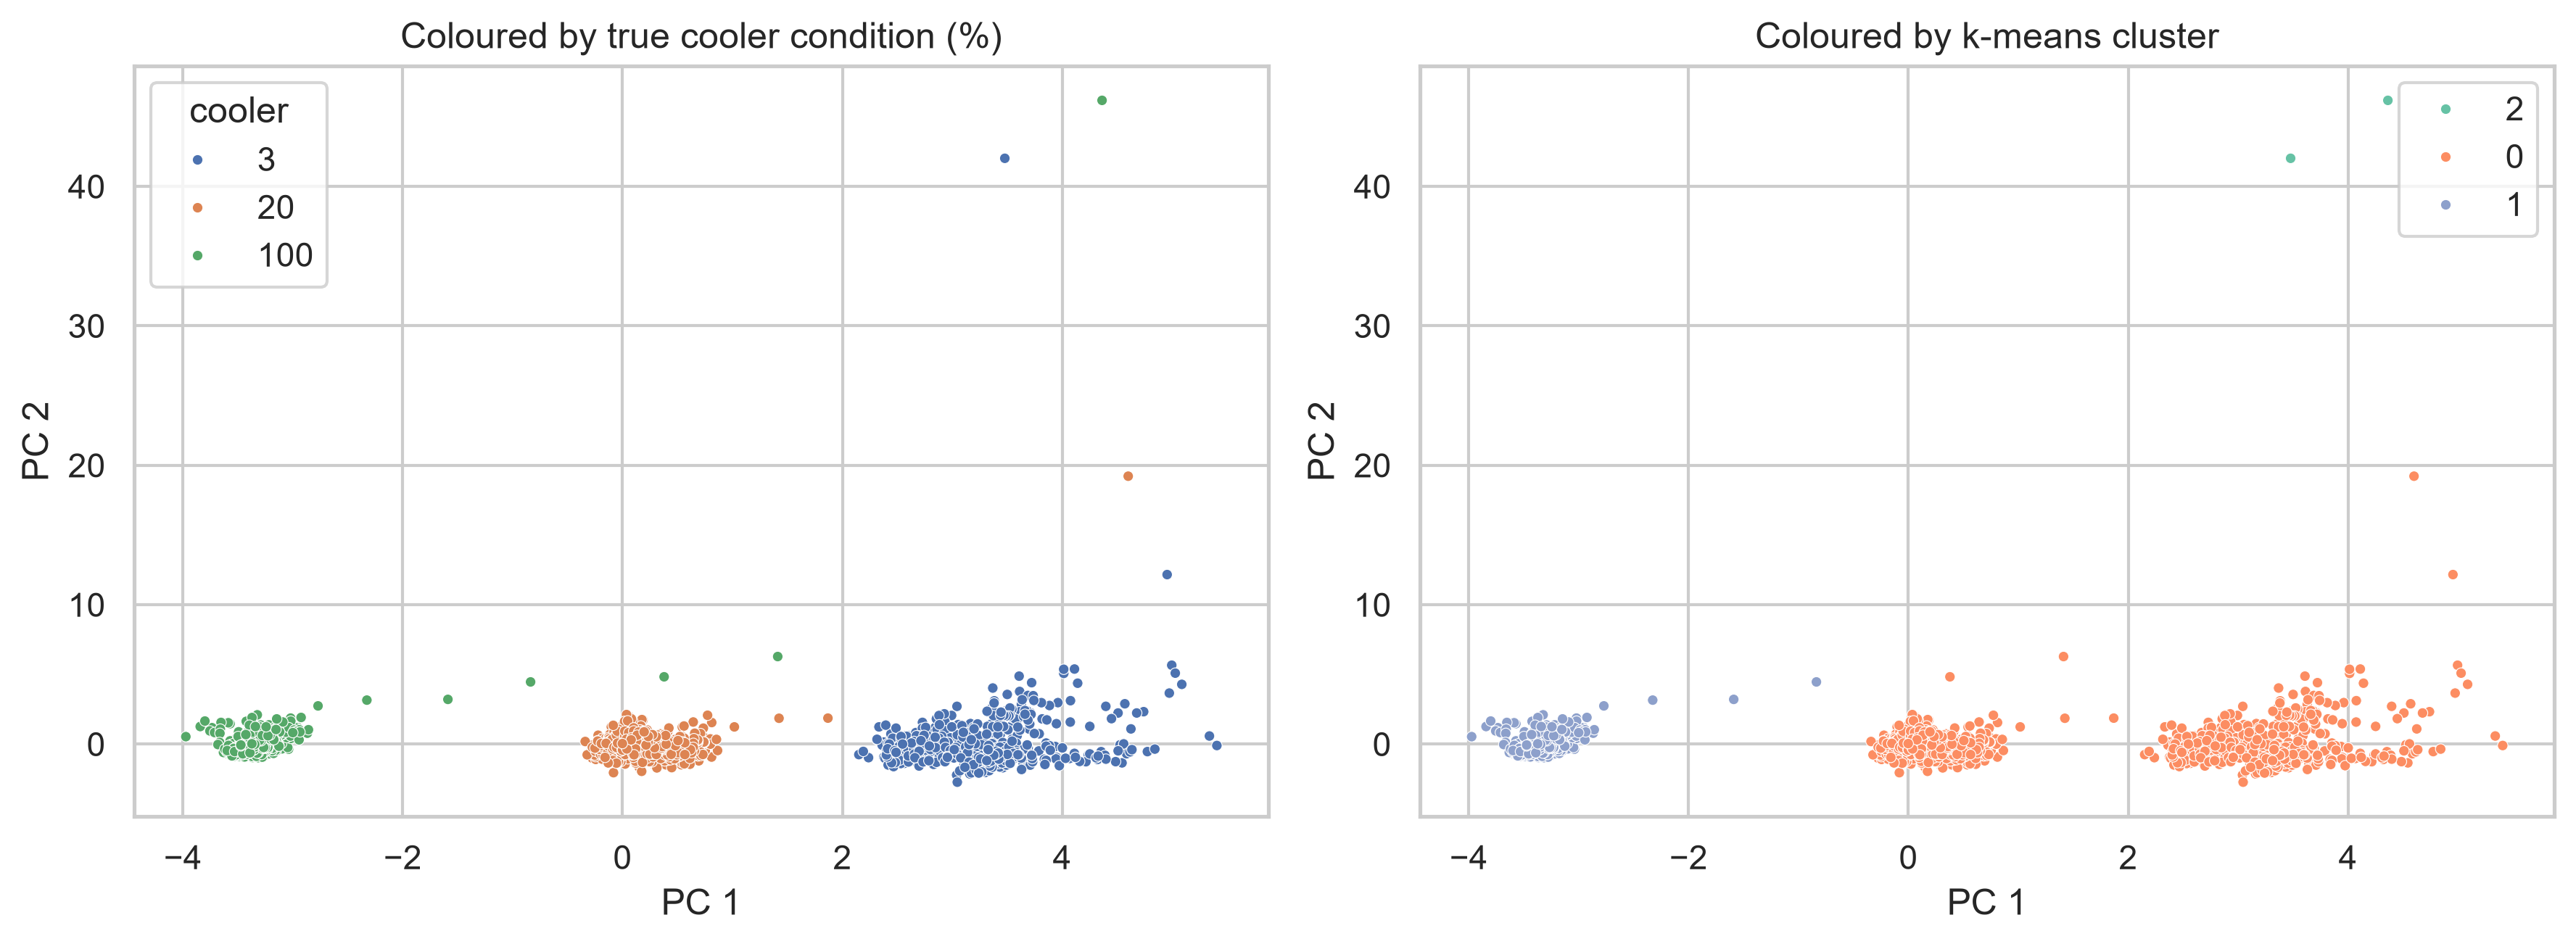
\includegraphics[keepaspectratio]{notebooks/09-unsupervised_files/figure-pdf/cell-8-output-4.png}}

\begin{longtable}[]{@{}llll@{}}
\toprule\noalign{}
cluster & 0 & 1 & 2 \\
cooler \% & & & \\
\midrule\noalign{}
\endhead
\bottomrule\noalign{}
\endlastfoot
3 & 731 & 0 & 1 \\
20 & 732 & 0 & 0 \\
100 & 2 & 738 & 1 \\
\end{longtable}

\textbf{Discussion.} Temperatures and cooling efficiency depend directly
on the cooler condition, so the operating states form well-separated
groups in the score plot, and k-means finds them without ever seeing the
labels. The cross-table compares clusters and true conditions. This is
the ideal case for unsupervised learning: the dominant source of
variation in the chosen features \emph{is} the condition of interest.
With features dominated by other influences, clusters would reflect
those instead -- feature choice is decisive.

\begin{tcolorbox}[enhanced jigsaw, colframe=quarto-callout-important-color-frame, toprule=.15mm, rightrule=.15mm, title=\textcolor{quarto-callout-important-color}{\faExclamation}\hspace{0.5em}{Key takeaways}, colbacktitle=quarto-callout-important-color!10!white, left=2mm, titlerule=0mm, bottomtitle=1mm, toptitle=1mm, opacityback=0, bottomrule=.15mm, breakable, arc=.35mm, opacitybacktitle=0.6, colback=white, coltitle=black, leftrule=.75mm]

\begin{itemize}
\tightlist
\item
  Unsupervised learning finds structure without labels: compression
  (PCA), grouping (clustering), deviations (anomaly detection).
\item
  PCA on standardised data summarises correlated sensors; T² and SPE
  monitor a process against its normal behaviour.
\item
  k-means needs a chosen \(k\) and spherical clusters; DBSCAN finds
  arbitrary shapes and noise.
\item
  Fit detectors on normal data, evaluate them with held-out normal data
  and a few labelled faults.
\end{itemize}

\end{tcolorbox}

\section{Exercises}\label{exercises-8}

\begin{enumerate}
\def\labelenumi{\arabic{enumi}.}
\tightlist
\item
  Split the passed SECOM runs into a training part (70 \%) and a test
  part (30 \%). Fit preprocessing, PCA and Isolation Forest on the
  training part only and evaluate on the test part plus all failed runs.
  How much does the AUC change compared with the optimistic evaluation?
\item
  Plot the first two principal component scores of SECOM coloured by
  pass/fail. Then run k-means with 2--6 clusters. Do clusters correspond
  to failures?
\item
  Hydraulic system: repeat the analysis with the pressure sensors
  \texttt{PS1}--\texttt{PS6} instead of the temperatures. Which
  component condition (cooler, valve, pump, accumulator) do the clusters
  now reflect best?
\item
  Discuss: why is failure detection in SECOM so hard, even though there
  are almost 600 sensors?
\end{enumerate}

\subsection{Solutions}\label{solutions-8}

\begin{tcolorbox}[enhanced jigsaw, colframe=quarto-callout-caution-color-frame, toprule=.15mm, rightrule=.15mm, title=\textcolor{quarto-callout-caution-color}{\faFire}\hspace{0.5em}{Solution to Exercise 1}, colbacktitle=quarto-callout-caution-color!10!white, left=2mm, titlerule=0mm, bottomtitle=1mm, toptitle=1mm, opacityback=0, bottomrule=.15mm, breakable, arc=.35mm, opacitybacktitle=0.6, colback=white, coltitle=black, leftrule=.75mm]

\begin{Shaded}
\begin{Highlighting}[]
\ImportTok{from}\NormalTok{ sklearn.model\_selection }\ImportTok{import}\NormalTok{ train\_test\_split}

\NormalTok{X\_pass, X\_fail }\OperatorTok{=}\NormalTok{ X[y }\OperatorTok{==} \OperatorTok{{-}}\DecValTok{1}\NormalTok{], X[y }\OperatorTok{==} \DecValTok{1}\NormalTok{]}
\NormalTok{X\_pass\_tr, X\_pass\_te }\OperatorTok{=}\NormalTok{ train\_test\_split(X\_pass, test\_size}\OperatorTok{=}\FloatTok{0.3}\NormalTok{, random\_state}\OperatorTok{=}\DecValTok{0}\NormalTok{)}

\NormalTok{prep2 }\OperatorTok{=}\NormalTok{ make\_pipeline(SimpleImputer(strategy}\OperatorTok{=}\StringTok{"median"}\NormalTok{), VarianceThreshold(}\FloatTok{1e{-}8}\NormalTok{), StandardScaler())}
\NormalTok{Z\_tr }\OperatorTok{=}\NormalTok{ prep2.fit\_transform(X\_pass\_tr)}
\NormalTok{X\_eval }\OperatorTok{=}\NormalTok{ pd.concat([X\_pass\_te, X\_fail])}
\NormalTok{y\_eval }\OperatorTok{=}\NormalTok{ np.r\_[np.zeros(}\BuiltInTok{len}\NormalTok{(X\_pass\_te)), np.ones(}\BuiltInTok{len}\NormalTok{(X\_fail))]}
\NormalTok{Z\_eval }\OperatorTok{=}\NormalTok{ prep2.transform(X\_eval)}

\NormalTok{iso2 }\OperatorTok{=}\NormalTok{ IsolationForest(n\_estimators}\OperatorTok{=}\DecValTok{300}\NormalTok{, random\_state}\OperatorTok{=}\DecValTok{0}\NormalTok{).fit(Z\_tr)}
\NormalTok{pca2 }\OperatorTok{=}\NormalTok{ PCA(k).fit(Z\_tr)}
\NormalTok{spe2 }\OperatorTok{=}\NormalTok{ np.}\BuiltInTok{sum}\NormalTok{((Z\_eval }\OperatorTok{{-}}\NormalTok{ pca2.inverse\_transform(pca2.transform(Z\_eval)))}\OperatorTok{**}\DecValTok{2}\NormalTok{, axis}\OperatorTok{=}\DecValTok{1}\NormalTok{)}
\BuiltInTok{print}\NormalTok{(}\SpecialStringTok{f"ROC AUC Isolation Forest (proper): }\SpecialCharTok{\{}\NormalTok{roc\_auc\_score(y\_eval, }\OperatorTok{{-}}\NormalTok{iso2.score\_samples(Z\_eval))}\SpecialCharTok{:.3f\}}\SpecialStringTok{"}\NormalTok{)}
\BuiltInTok{print}\NormalTok{(}\SpecialStringTok{f"ROC AUC SPE (proper):              }\SpecialCharTok{\{}\NormalTok{roc\_auc\_score(y\_eval, spe2)}\SpecialCharTok{:.3f\}}\SpecialStringTok{"}\NormalTok{)}
\end{Highlighting}
\end{Shaded}

\begin{verbatim}
ROC AUC Isolation Forest (proper): 0.577
ROC AUC SPE (proper):              0.596
\end{verbatim}

The SPE in particular drops when evaluated properly: the PCA model
reconstructs its own training runs better than new runs, so in the
optimistic evaluation the normal runs looked ``too normal'' compared
with the failed ones. Proper separation of training and evaluation data
is just as important in unsupervised as in supervised learning.

\end{tcolorbox}

\begin{tcolorbox}[enhanced jigsaw, colframe=quarto-callout-caution-color-frame, toprule=.15mm, rightrule=.15mm, title=\textcolor{quarto-callout-caution-color}{\faFire}\hspace{0.5em}{Solution to Exercise 2}, colbacktitle=quarto-callout-caution-color!10!white, left=2mm, titlerule=0mm, bottomtitle=1mm, toptitle=1mm, opacityback=0, bottomrule=.15mm, breakable, arc=.35mm, opacitybacktitle=0.6, colback=white, coltitle=black, leftrule=.75mm]

\begin{Shaded}
\begin{Highlighting}[]
\NormalTok{scores\_s }\OperatorTok{=}\NormalTok{ pca\_k.transform(prep.transform(X))[:, :}\DecValTok{2}\NormalTok{]}
\NormalTok{plt.scatter(scores\_s[:, }\DecValTok{0}\NormalTok{], scores\_s[:, }\DecValTok{1}\NormalTok{], c}\OperatorTok{=}\NormalTok{(y }\OperatorTok{==} \DecValTok{1}\NormalTok{), cmap}\OperatorTok{=}\StringTok{"coolwarm"}\NormalTok{, s}\OperatorTok{=}\DecValTok{8}\NormalTok{, alpha}\OperatorTok{=}\FloatTok{0.6}\NormalTok{)}
\NormalTok{plt.xlabel(}\StringTok{"PC 1"}\NormalTok{)}\OperatorTok{;}\NormalTok{ plt.ylabel(}\StringTok{"PC 2"}\NormalTok{)}\OperatorTok{;}\NormalTok{ plt.title(}\StringTok{"SECOM scores, red = fail"}\NormalTok{)}
\NormalTok{plt.show()}

\NormalTok{Zall }\OperatorTok{=}\NormalTok{ prep.transform(X)}
\ControlFlowTok{for}\NormalTok{ k\_ }\KeywordTok{in} \BuiltInTok{range}\NormalTok{(}\DecValTok{2}\NormalTok{, }\DecValTok{7}\NormalTok{):}
\NormalTok{    lab }\OperatorTok{=}\NormalTok{ KMeans(k\_, n\_init}\OperatorTok{=}\DecValTok{10}\NormalTok{, random\_state}\OperatorTok{=}\DecValTok{0}\NormalTok{).fit\_predict(Zall)}
\NormalTok{    rates }\OperatorTok{=}\NormalTok{ pd.Series(y.values }\OperatorTok{==} \DecValTok{1}\NormalTok{).groupby(lab).mean()}
    \BuiltInTok{print}\NormalTok{(}\SpecialStringTok{f"k = }\SpecialCharTok{\{}\NormalTok{k\_}\SpecialCharTok{\}}\SpecialStringTok{: failure rate per cluster"}\NormalTok{, rates.}\BuiltInTok{round}\NormalTok{(}\DecValTok{3}\NormalTok{).tolist())}
\end{Highlighting}
\end{Shaded}

\pandocbounded{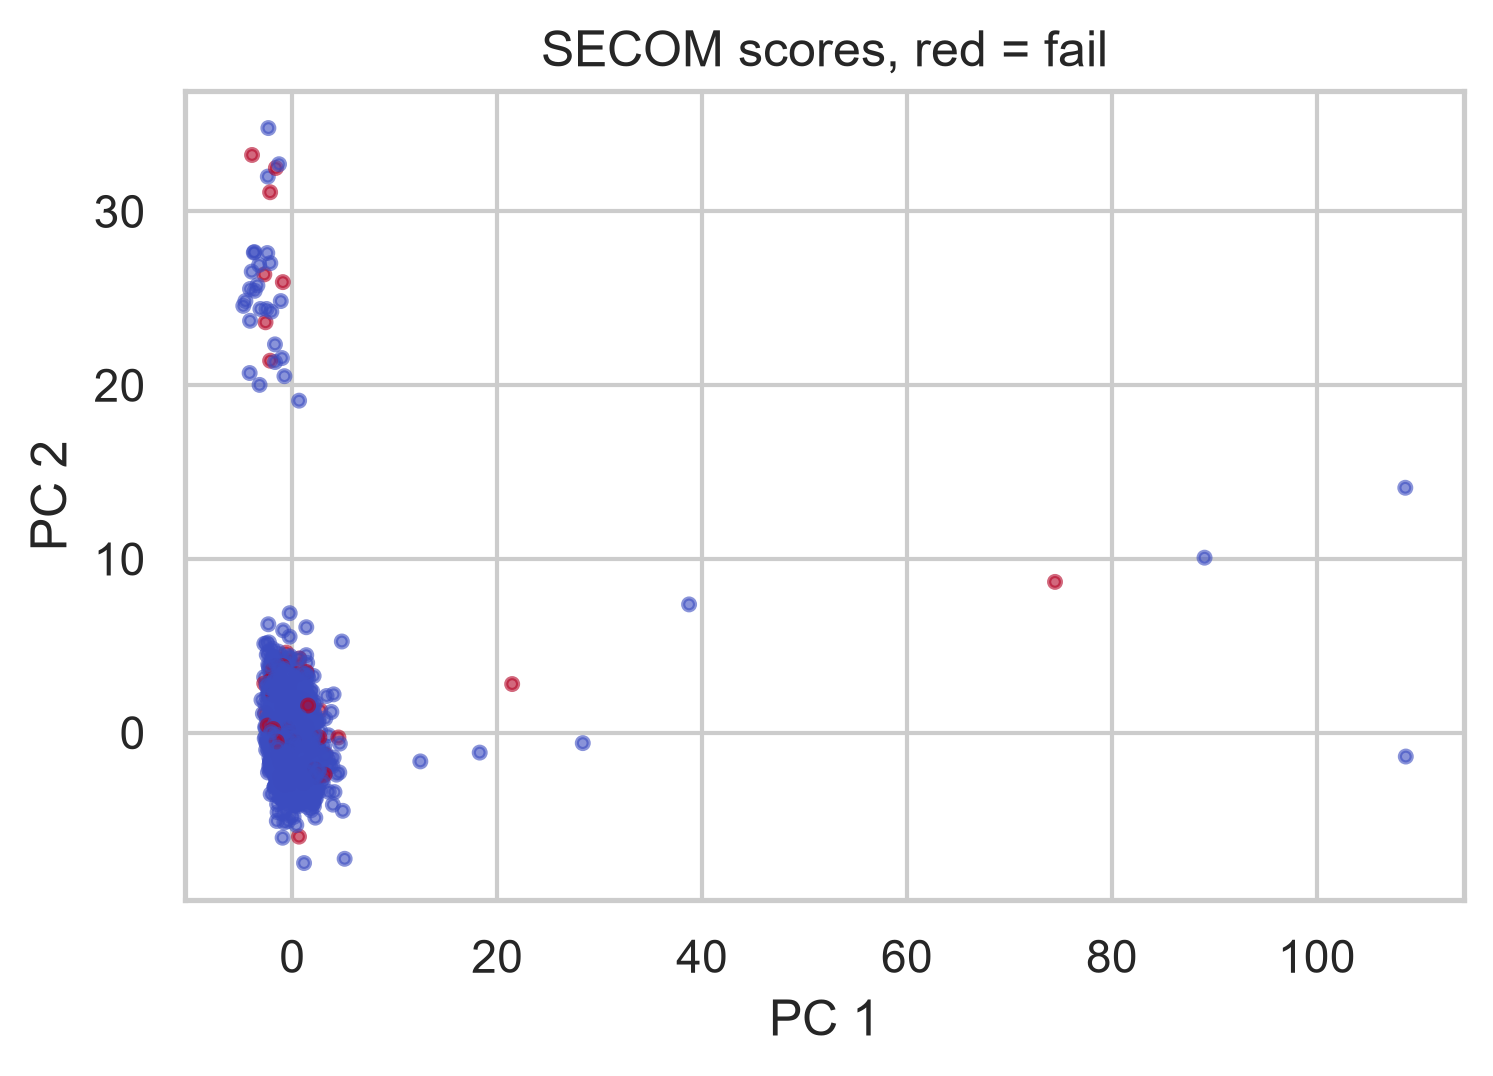
\includegraphics[keepaspectratio]{notebooks/09-unsupervised_files/figure-pdf/cell-10-output-1.png}}

\begin{verbatim}
C:\Tools\Anaconda\Lib\site-packages\sklearn\cluster\_kmeans.py:1424: UserWarning: KMeans is known to have a memory leak on Windows with MKL, when there are less chunks than available threads. You can avoid it by setting the environment variable OMP_NUM_THREADS=7.
  warnings.warn(
C:\Tools\Anaconda\Lib\site-packages\sklearn\cluster\_kmeans.py:1424: UserWarning: KMeans is known to have a memory leak on Windows with MKL, when there are less chunks than available threads. You can avoid it by setting the environment variable OMP_NUM_THREADS=7.
  warnings.warn(
\end{verbatim}

\begin{verbatim}
k = 2: failure rate per cluster [0.2, 0.066]
k = 3: failure rate per cluster [0.049, 0.084, 0.25]
\end{verbatim}

\begin{verbatim}
C:\Tools\Anaconda\Lib\site-packages\sklearn\cluster\_kmeans.py:1424: UserWarning: KMeans is known to have a memory leak on Windows with MKL, when there are less chunks than available threads. You can avoid it by setting the environment variable OMP_NUM_THREADS=7.
  warnings.warn(
C:\Tools\Anaconda\Lib\site-packages\sklearn\cluster\_kmeans.py:1424: UserWarning: KMeans is known to have a memory leak on Windows with MKL, when there are less chunks than available threads. You can avoid it by setting the environment variable OMP_NUM_THREADS=7.
  warnings.warn(
\end{verbatim}

\begin{verbatim}
k = 4: failure rate per cluster [0.08, 0.25, 0.047, 0.212]
k = 5: failure rate per cluster [0.06, 0.072, 0.05, 0.25, 0.219]
k = 6: failure rate per cluster [0.137, 0.041, 0.055, 0.219, 0.051, 0.25]
\end{verbatim}

\begin{verbatim}
C:\Tools\Anaconda\Lib\site-packages\sklearn\cluster\_kmeans.py:1424: UserWarning: KMeans is known to have a memory leak on Windows with MKL, when there are less chunks than available threads. You can avoid it by setting the environment variable OMP_NUM_THREADS=7.
  warnings.warn(
\end{verbatim}

The failed runs are scattered among the passed ones in the first two
components, and the failure rate per cluster stays close to the overall
rate of about 6--7 \%. The dominant sources of variation in SECOM
(e.g.~tool or recipe changes) are not related to the pass/fail outcome.
Clustering finds the largest structure in the data -- which need not be
the structure we are interested in.

\end{tcolorbox}

\begin{tcolorbox}[enhanced jigsaw, colframe=quarto-callout-caution-color-frame, toprule=.15mm, rightrule=.15mm, title=\textcolor{quarto-callout-caution-color}{\faFire}\hspace{0.5em}{Solution to Exercise 3}, colbacktitle=quarto-callout-caution-color!10!white, left=2mm, titlerule=0mm, bottomtitle=1mm, toptitle=1mm, opacityback=0, bottomrule=.15mm, breakable, arc=.35mm, opacitybacktitle=0.6, colback=white, coltitle=black, leftrule=.75mm]

\begin{Shaded}
\begin{Highlighting}[]
\ControlFlowTok{with}\NormalTok{ zipfile.ZipFile(hz) }\ImportTok{as}\NormalTok{ z:}
\NormalTok{    ps }\OperatorTok{=}\NormalTok{ \{s: read\_sensor(z, }\SpecialStringTok{f"}\SpecialCharTok{\{}\NormalTok{s}\SpecialCharTok{\}}\SpecialStringTok{.txt"}\NormalTok{) }\ControlFlowTok{for}\NormalTok{ s }\KeywordTok{in}\NormalTok{ [}\StringTok{"PS1"}\NormalTok{, }\StringTok{"PS2"}\NormalTok{, }\StringTok{"PS3"}\NormalTok{, }\StringTok{"PS4"}\NormalTok{, }\StringTok{"PS5"}\NormalTok{, }\StringTok{"PS6"}\NormalTok{]\}}
\NormalTok{feat\_ps }\OperatorTok{=}\NormalTok{ pd.DataFrame(\{}\SpecialStringTok{f"}\SpecialCharTok{\{}\NormalTok{s}\SpecialCharTok{\}}\SpecialStringTok{\_}\SpecialCharTok{\{}\NormalTok{stat}\SpecialCharTok{\}}\SpecialStringTok{"}\NormalTok{: }\BuiltInTok{getattr}\NormalTok{(np, stat)(v, axis}\OperatorTok{=}\DecValTok{1}\NormalTok{)}
                        \ControlFlowTok{for}\NormalTok{ s, v }\KeywordTok{in}\NormalTok{ ps.items() }\ControlFlowTok{for}\NormalTok{ stat }\KeywordTok{in}\NormalTok{ [}\StringTok{"mean"}\NormalTok{, }\StringTok{"std"}\NormalTok{, }\StringTok{"max"}\NormalTok{]\})}
\NormalTok{Zp }\OperatorTok{=}\NormalTok{ StandardScaler().fit\_transform(feat\_ps)}
\NormalTok{lab\_ps }\OperatorTok{=}\NormalTok{ KMeans(}\DecValTok{4}\NormalTok{, n\_init}\OperatorTok{=}\DecValTok{10}\NormalTok{, random\_state}\OperatorTok{=}\DecValTok{0}\NormalTok{).fit\_predict(Zp)}

\ImportTok{from}\NormalTok{ sklearn.metrics }\ImportTok{import}\NormalTok{ adjusted\_rand\_score}
\NormalTok{\{c: }\BuiltInTok{round}\NormalTok{(adjusted\_rand\_score(profile[c], lab\_ps), }\DecValTok{3}\NormalTok{) }\ControlFlowTok{for}\NormalTok{ c }\KeywordTok{in}\NormalTok{ [}\StringTok{"cooler"}\NormalTok{, }\StringTok{"valve"}\NormalTok{, }\StringTok{"pump\_leak"}\NormalTok{, }\StringTok{"accumulator"}\NormalTok{]\}}
\end{Highlighting}
\end{Shaded}

\begin{verbatim}
C:\Tools\Anaconda\Lib\site-packages\sklearn\cluster\_kmeans.py:1424: UserWarning: KMeans is known to have a memory leak on Windows with MKL, when there are less chunks than available threads. You can avoid it by setting the environment variable OMP_NUM_THREADS=9.
  warnings.warn(
\end{verbatim}

\begin{verbatim}
{'cooler': 0.585, 'valve': 0.034, 'pump_leak': 0.094, 'accumulator': 0.04}
\end{verbatim}

The adjusted Rand index (0 = random agreement, 1 = identical grouping)
shows which component condition the clusters reflect. Pressure features
respond strongly to the valve condition (switching behaviour) and the
accumulator pre-charge pressure, while the temperatures reflected the
cooler. Different sensors ``see'' different faults -- a central insight
for designing condition monitoring systems.

\end{tcolorbox}

\begin{tcolorbox}[enhanced jigsaw, colframe=quarto-callout-caution-color-frame, toprule=.15mm, rightrule=.15mm, title=\textcolor{quarto-callout-caution-color}{\faFire}\hspace{0.5em}{Solution to Exercise 4}, colbacktitle=quarto-callout-caution-color!10!white, left=2mm, titlerule=0mm, bottomtitle=1mm, toptitle=1mm, opacityback=0, bottomrule=.15mm, breakable, arc=.35mm, opacitybacktitle=0.6, colback=white, coltitle=black, leftrule=.75mm]

Possible reasons: (1) the measurements are summary values per run and
may not capture the physical cause of the failure; (2) the failures may
have several different causes, so there is no single ``failure
direction''; (3) many features are noise, and in high dimensions the
distance to normal data grows for \emph{every} point, which dilutes
anomaly scores; (4) only about 100 failures are available, and labels
may be noisy; (5) part of the failures may originate in later process
steps that are not measured at all. More sensors do not help if they do
not measure the right thing.

\end{tcolorbox}

\chapter{Signals and Feature
Engineering}\label{signals-and-feature-engineering}

Condition monitoring systems record vibration, current, pressure or
acoustic signals at sampling rates of several kilohertz. A single minute
of vibration data from one accelerometer at 12 kHz contains 720,000
numbers. Machine learning models cannot -- and should not -- work on
such raw data directly. They need a small set of \textbf{features} that
capture the information relevant for the question at hand.

This chapter shows how to get from a raw signal to meaningful features.
We look at signals in the time and in the frequency domain, use the
physics of rolling bearings to know \emph{where} in the spectrum a fault
should appear, and compute statistical features that summarise a signal
window. Feature engineering is where engineering knowledge pays off most
in data science.

\textbf{Scenario: a cheap sensor for the pump station}

A water utility operates dozens of pumps with rolling bearings. A full
condition monitoring system is too expensive, but the maintenance team
could fit each pump with a low-cost vibration sensor that computes a
single number per second and raises an alarm above a threshold. The team
asks: which number, which threshold -- and will it work?

\textbf{Your decision:} Is a simple threshold on one statistical feature
good enough to detect an inner-race fault, and which threshold do you
set?

\textbf{Learning goals.} After this chapter you can

\begin{itemize}
\tightlist
\item
  explain sampling, the Nyquist frequency and aliasing,
\item
  compute and interpret amplitude spectra with the FFT, including
  frequency resolution and leakage,
\item
  calculate characteristic bearing fault frequencies and relate spectral
  peaks to them,
\item
  extract statistical features (RMS, peak, crest factor, kurtosis) from
  signal windows,
\item
  split windowed data correctly for training and testing,
\item
  (extension) explain and apply envelope analysis.
\end{itemize}

\textbf{Datasets in this chapter}

\begin{itemize}
\tightlist
\item
  \href{https://engineering.case.edu/bearingdatacenter}{CWRU Bearing
  Data Center}
\item
  \href{https://archive.ics.uci.edu/dataset/447/condition+monitoring+of+hydraulic+systems}{Condition
  Monitoring of Hydraulic Systems (UCI)}
\end{itemize}

\section{Sampling and aliasing}\label{sampling-and-aliasing}

A sensor signal is continuous; the data acquisition system samples it at
discrete times \(t_n = n/f_s\) with the \textbf{sampling rate} \(f_s\).

\begin{tcolorbox}[enhanced jigsaw, colframe=quarto-callout-important-color-frame, toprule=.15mm, rightrule=.15mm, title=\textcolor{quarto-callout-important-color}{\faExclamation}\hspace{0.5em}{Sampling theorem (Nyquist--Shannon)}, colbacktitle=quarto-callout-important-color!10!white, left=2mm, titlerule=0mm, bottomtitle=1mm, toptitle=1mm, opacityback=0, bottomrule=.15mm, breakable, arc=.35mm, opacitybacktitle=0.6, colback=white, coltitle=black, leftrule=.75mm]

A signal can be reconstructed from its samples if it contains no
frequencies at or above half the sampling rate, the \textbf{Nyquist
frequency} \(f_N = f_s/2\). Frequencies above \(f_N\) are not lost
silently -- they are folded back and appear as false lower frequencies
(\textbf{aliasing}).

\end{tcolorbox}

\begin{figure}[H]

\centering{

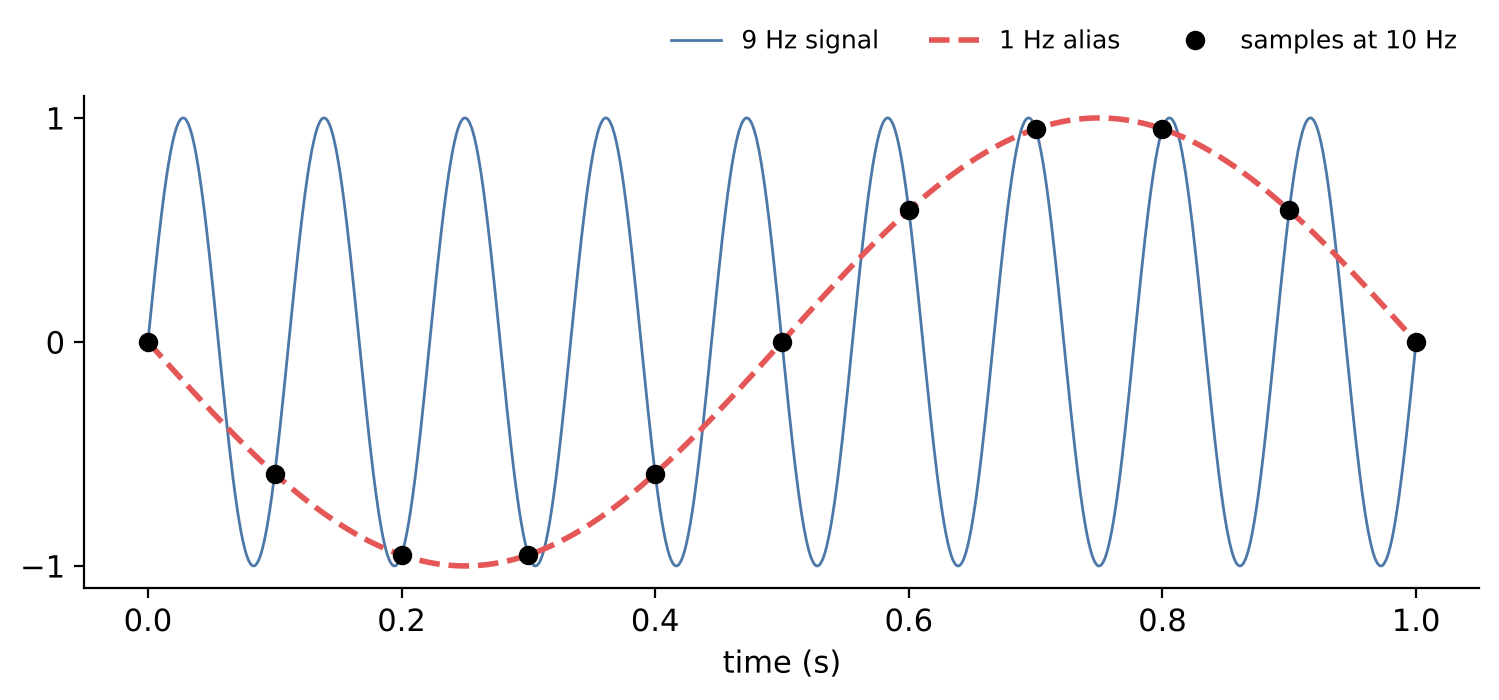
\includegraphics[width=0.85\linewidth,height=\textheight,keepaspectratio]{notebooks/images/aliasing.png}

}

\caption{\label{fig-aliasing}Aliasing. A 9 Hz sine sampled at 10 Hz
(dots) produces exactly the same samples as a 1 Hz sine. After sampling,
the two cannot be distinguished.}

\end{figure}%

A component at frequency \(f\) with \(f_N < f < f_s\) appears at
\(|f - f_s|\). This is why data acquisition systems use an analogue
\textbf{anti-aliasing filter} before the A/D converter. Once aliasing
has happened, no digital processing can undo it.

\section{The frequency domain}\label{the-frequency-domain}

Rotating machines produce periodic excitations: imbalance at the shaft
frequency, gear meshing at the tooth frequency, bearing defects at
characteristic frequencies. In the time domain these components overlap;
in the frequency domain they separate into peaks.

\begin{tcolorbox}[enhanced jigsaw, colframe=quarto-callout-note-color-frame, toprule=.15mm, rightrule=.15mm, title=\textcolor{quarto-callout-note-color}{\faInfo}\hspace{0.5em}{Definition: Discrete Fourier transform and amplitude spectrum}, colbacktitle=quarto-callout-note-color!10!white, left=2mm, titlerule=0mm, bottomtitle=1mm, toptitle=1mm, opacityback=0, bottomrule=.15mm, breakable, arc=.35mm, opacitybacktitle=0.6, colback=white, coltitle=black, leftrule=.75mm]

For \(N\) samples \(x_0, \dots, x_{N-1}\), the discrete Fourier
transform is
\[X_k = \sum_{n=0}^{N-1} x_n\, e^{-2\pi i\,kn/N}, \qquad k = 0, \dots, N-1,\]
computed efficiently by the \textbf{fast Fourier transform (FFT)}. Bin
\(k\) corresponds to the frequency \(f_k = k\,f_s/N\). The single-sided
\textbf{amplitude spectrum} \(A_k = 2|X_k|/N\) (for \(0 < k < N/2\))
gives the amplitude of a sine component at \(f_k\).

\end{tcolorbox}

Two practical facts:

\begin{itemize}
\tightlist
\item
  \textbf{Frequency resolution} \(\Delta f = f_s/N = 1/T\): it depends
  only on the measurement duration \(T\). To separate two peaks 1 Hz
  apart, you need at least one second of data.
\item
  \textbf{Leakage:} the FFT assumes the signal window repeats
  periodically. If a component does not complete an integer number of
  periods in the window, its energy ``leaks'' into neighbouring bins.
  Multiplying the window by a smooth \textbf{window function}
  (e.g.~Hann) reduces leakage at the price of slightly wider peaks.
\end{itemize}

\section{Bearing fault frequencies}\label{bearing-fault-frequencies}

When a rolling element passes a local defect on a raceway, it produces a
short impact. These impacts repeat at frequencies that follow from the
bearing geometry: with shaft frequency \(f_r\), number of rolling
elements \(n_b\), rolling element diameter \(d\), pitch diameter \(D\)
and contact angle \(\phi\),

\[\text{BPFO} = \frac{n_b f_r}{2}\left(1 - \frac{d}{D}\cos\phi\right), \qquad \text{BPFI} = \frac{n_b f_r}{2}\left(1 + \frac{d}{D}\cos\phi\right).\]

BPFO and BPFI are the \emph{ball pass frequencies} of the outer and
inner race. For the drive-end bearing of the CWRU test rig (SKF 6205),
the CWRU documentation gives BPFI ≈ 5.415 \(f_r\) and BPFO ≈ 3.585
\(f_r\) -- check the bearing specification page before relying on these
factors.

\begin{tcolorbox}[enhanced jigsaw, colframe=quarto-callout-tip-color-frame, toprule=.15mm, rightrule=.15mm, title=\textcolor{quarto-callout-tip-color}{\faLightbulb}\hspace{0.5em}{Engineering practice: let physics tell you where to look}, colbacktitle=quarto-callout-tip-color!10!white, left=2mm, titlerule=0mm, bottomtitle=1mm, toptitle=1mm, opacityback=0, bottomrule=.15mm, breakable, arc=.35mm, opacitybacktitle=0.6, colback=white, coltitle=black, leftrule=.75mm]

Knowing the fault frequencies turns a vague search (``is the spectrum
different?'') into a targeted test (``is there a peak at BPFI and its
harmonics?''). Features built from physics -- the amplitude at BPFI, the
energy in a resonance band -- are more robust and easier to explain than
features found by blind search.

\end{tcolorbox}

\section{Statistical features of a signal
window}\label{statistical-features-of-a-signal-window}

\begin{tcolorbox}[enhanced jigsaw, colframe=quarto-callout-note-color-frame, toprule=.15mm, rightrule=.15mm, title=\textcolor{quarto-callout-note-color}{\faInfo}\hspace{0.5em}{Definition: Common time-domain features}, colbacktitle=quarto-callout-note-color!10!white, left=2mm, titlerule=0mm, bottomtitle=1mm, toptitle=1mm, opacityback=0, bottomrule=.15mm, breakable, arc=.35mm, opacitybacktitle=0.6, colback=white, coltitle=black, leftrule=.75mm]

For a window \(x_1, \dots, x_N\):

\begin{itemize}
\tightlist
\item
  \textbf{RMS} \(= \sqrt{\frac{1}{N}\sum x_i^2}\) -- overall vibration
  energy,
\item
  \textbf{peak} \(= \max |x_i|\),
\item
  \textbf{crest factor} \(=\) peak / RMS -- impulsiveness,
\item
  \textbf{kurtosis} \(= m_4/m_2^2 - 3\) (excess kurtosis), with the
  central moments \(m_r = \frac1N\sum_{i=1}^N (x_i - \bar x)^r\) --
  ``spikiness''; 0 for a normal distribution, large for signals with
  short impacts,
\item
  \textbf{skewness} -- asymmetry of the amplitude distribution.
\end{itemize}

\end{tcolorbox}

Early bearing damage produces short impacts: kurtosis and crest factor
rise while the RMS hardly changes. As damage progresses and spreads, the
impacts become less distinct, kurtosis may fall again and RMS rises -- a
reason to use several features together.

\begin{tcolorbox}[enhanced jigsaw, colframe=quarto-callout-warning-color-frame, toprule=.15mm, rightrule=.15mm, title=\textcolor{quarto-callout-warning-color}{\faExclamationTriangle}\hspace{0.5em}{Pitfall: splitting windows of the same recording}, colbacktitle=quarto-callout-warning-color!10!white, left=2mm, titlerule=0mm, bottomtitle=1mm, toptitle=1mm, opacityback=0, bottomrule=.15mm, breakable, arc=.35mm, opacitybacktitle=0.6, colback=white, coltitle=black, leftrule=.75mm]

When a long recording is cut into windows, neighbouring windows are
almost identical. If windows of the same recording end up in both
training and test set, the model recognises the \emph{recording}, not
the fault -- the test accuracy is meaningless. Split by recording,
machine or time period (e.g.~with \texttt{GroupKFold}), never randomly
by window.

\end{tcolorbox}

\begin{Shaded}
\begin{Highlighting}[]
\CommentTok{\# Setup: works locally and in Google Colab}
\ImportTok{import}\NormalTok{ numpy }\ImportTok{as}\NormalTok{ np}
\ImportTok{import}\NormalTok{ pandas }\ImportTok{as}\NormalTok{ pd}
\ImportTok{import}\NormalTok{ matplotlib.pyplot }\ImportTok{as}\NormalTok{ plt}
\ImportTok{import}\NormalTok{ seaborn }\ImportTok{as}\NormalTok{ sns}
\ImportTok{from}\NormalTok{ scipy }\ImportTok{import}\NormalTok{ signal, stats}
\ImportTok{from}\NormalTok{ scipy.io }\ImportTok{import}\NormalTok{ loadmat}

\NormalTok{sns.set\_theme(style}\OperatorTok{=}\StringTok{"whitegrid"}\NormalTok{)}
\end{Highlighting}
\end{Shaded}

\begin{Shaded}
\begin{Highlighting}[]
\ImportTok{from}\NormalTok{ pathlib }\ImportTok{import}\NormalTok{ Path}
\ImportTok{import}\NormalTok{ requests}

\NormalTok{DATA }\OperatorTok{=}\NormalTok{ Path(}\StringTok{"data"}\NormalTok{)}
\NormalTok{DATA.mkdir(exist\_ok}\OperatorTok{=}\VariableTok{True}\NormalTok{)}

\KeywordTok{def}\NormalTok{ download(url, fname}\OperatorTok{=}\VariableTok{None}\NormalTok{):}
    \CommentTok{"""Download a file once and cache it in ./data."""}
\NormalTok{    path }\OperatorTok{=}\NormalTok{ DATA }\OperatorTok{/}\NormalTok{ (fname }\KeywordTok{or}\NormalTok{ url.split(}\StringTok{"/"}\NormalTok{)[}\OperatorTok{{-}}\DecValTok{1}\NormalTok{])}
    \ControlFlowTok{if} \KeywordTok{not}\NormalTok{ path.exists():}
\NormalTok{        r }\OperatorTok{=}\NormalTok{ requests.get(url, timeout}\OperatorTok{=}\DecValTok{120}\NormalTok{)}
\NormalTok{        r.raise\_for\_status()}
\NormalTok{        path.write\_bytes(r.content)}
    \ControlFlowTok{return}\NormalTok{ path}
\end{Highlighting}
\end{Shaded}

\section{Live coding: healthy vs.~inner-race
fault}\label{live-coding-healthy-vs.-inner-race-fault}

The Case Western Reserve University (CWRU) bearing data are a widely
used benchmark. Faults of defined size were introduced into the bearings
of a 2 hp motor test rig by electro-discharge machining; vibration was
measured with accelerometers at the drive end and fan end. We use two
files: normal baseline (\texttt{97.mat}) and a 0.007-inch inner race
fault at the drive end (\texttt{105.mat}), both at 0 hp motor load
(approx. 1797 rpm).

\textbf{Check the file numbers and the sampling rates (12 kHz or 48 kHz)
on the CWRU download pages before using them} -- the values below are
set accordingly and marked.

\begin{Shaded}
\begin{Highlighting}[]
\NormalTok{FILES }\OperatorTok{=}\NormalTok{ \{}\StringTok{"normal"}\NormalTok{: (}\StringTok{"97.mat"}\NormalTok{, }\DecValTok{48\_000}\NormalTok{), }\StringTok{"inner race"}\NormalTok{: (}\StringTok{"105.mat"}\NormalTok{, }\DecValTok{12\_000}\NormalTok{)\}   }\CommentTok{\# file, sampling rate (Hz) – verify!}
\NormalTok{BASE\_URL }\OperatorTok{=} \StringTok{"https://engineering.case.edu/sites/default/files/"}

\NormalTok{signals }\OperatorTok{=}\NormalTok{ \{\}}
\ControlFlowTok{for}\NormalTok{ label, (fname, fs) }\KeywordTok{in}\NormalTok{ FILES.items():}
\NormalTok{    mat }\OperatorTok{=}\NormalTok{ loadmat(download(BASE\_URL }\OperatorTok{+}\NormalTok{ fname))}
\NormalTok{    key }\OperatorTok{=} \BuiltInTok{next}\NormalTok{(k }\ControlFlowTok{for}\NormalTok{ k }\KeywordTok{in}\NormalTok{ mat }\ControlFlowTok{if}\NormalTok{ k.endswith(}\StringTok{"\_DE\_time"}\NormalTok{))     }\CommentTok{\# drive{-}end accelerometer}
\NormalTok{    signals[label] }\OperatorTok{=}\NormalTok{ (mat[key].ravel(), fs)}

\NormalTok{fig, axes }\OperatorTok{=}\NormalTok{ plt.subplots(}\DecValTok{2}\NormalTok{, }\DecValTok{1}\NormalTok{, figsize}\OperatorTok{=}\NormalTok{(}\DecValTok{10}\NormalTok{, }\DecValTok{5}\NormalTok{), sharex}\OperatorTok{=}\VariableTok{True}\NormalTok{)}
\ControlFlowTok{for}\NormalTok{ ax, (label, (x, fs)) }\KeywordTok{in} \BuiltInTok{zip}\NormalTok{(axes, signals.items()):}
\NormalTok{    t }\OperatorTok{=}\NormalTok{ np.arange(}\BuiltInTok{len}\NormalTok{(x)) }\OperatorTok{/}\NormalTok{ fs}
\NormalTok{    ax.plot(t, x, lw}\OperatorTok{=}\FloatTok{0.5}\NormalTok{)}\OperatorTok{;}\NormalTok{ ax.}\BuiltInTok{set}\NormalTok{(title}\OperatorTok{=}\NormalTok{label, ylabel}\OperatorTok{=}\StringTok{"Acceleration (g)"}\NormalTok{)}
\NormalTok{axes[}\DecValTok{1}\NormalTok{].}\BuiltInTok{set}\NormalTok{(xlim}\OperatorTok{=}\NormalTok{(}\DecValTok{0}\NormalTok{, }\FloatTok{0.2}\NormalTok{), xlabel}\OperatorTok{=}\StringTok{"Time (s)"}\NormalTok{)}
\NormalTok{plt.tight\_layout()}\OperatorTok{;}\NormalTok{ plt.show()}
\end{Highlighting}
\end{Shaded}

\pandocbounded{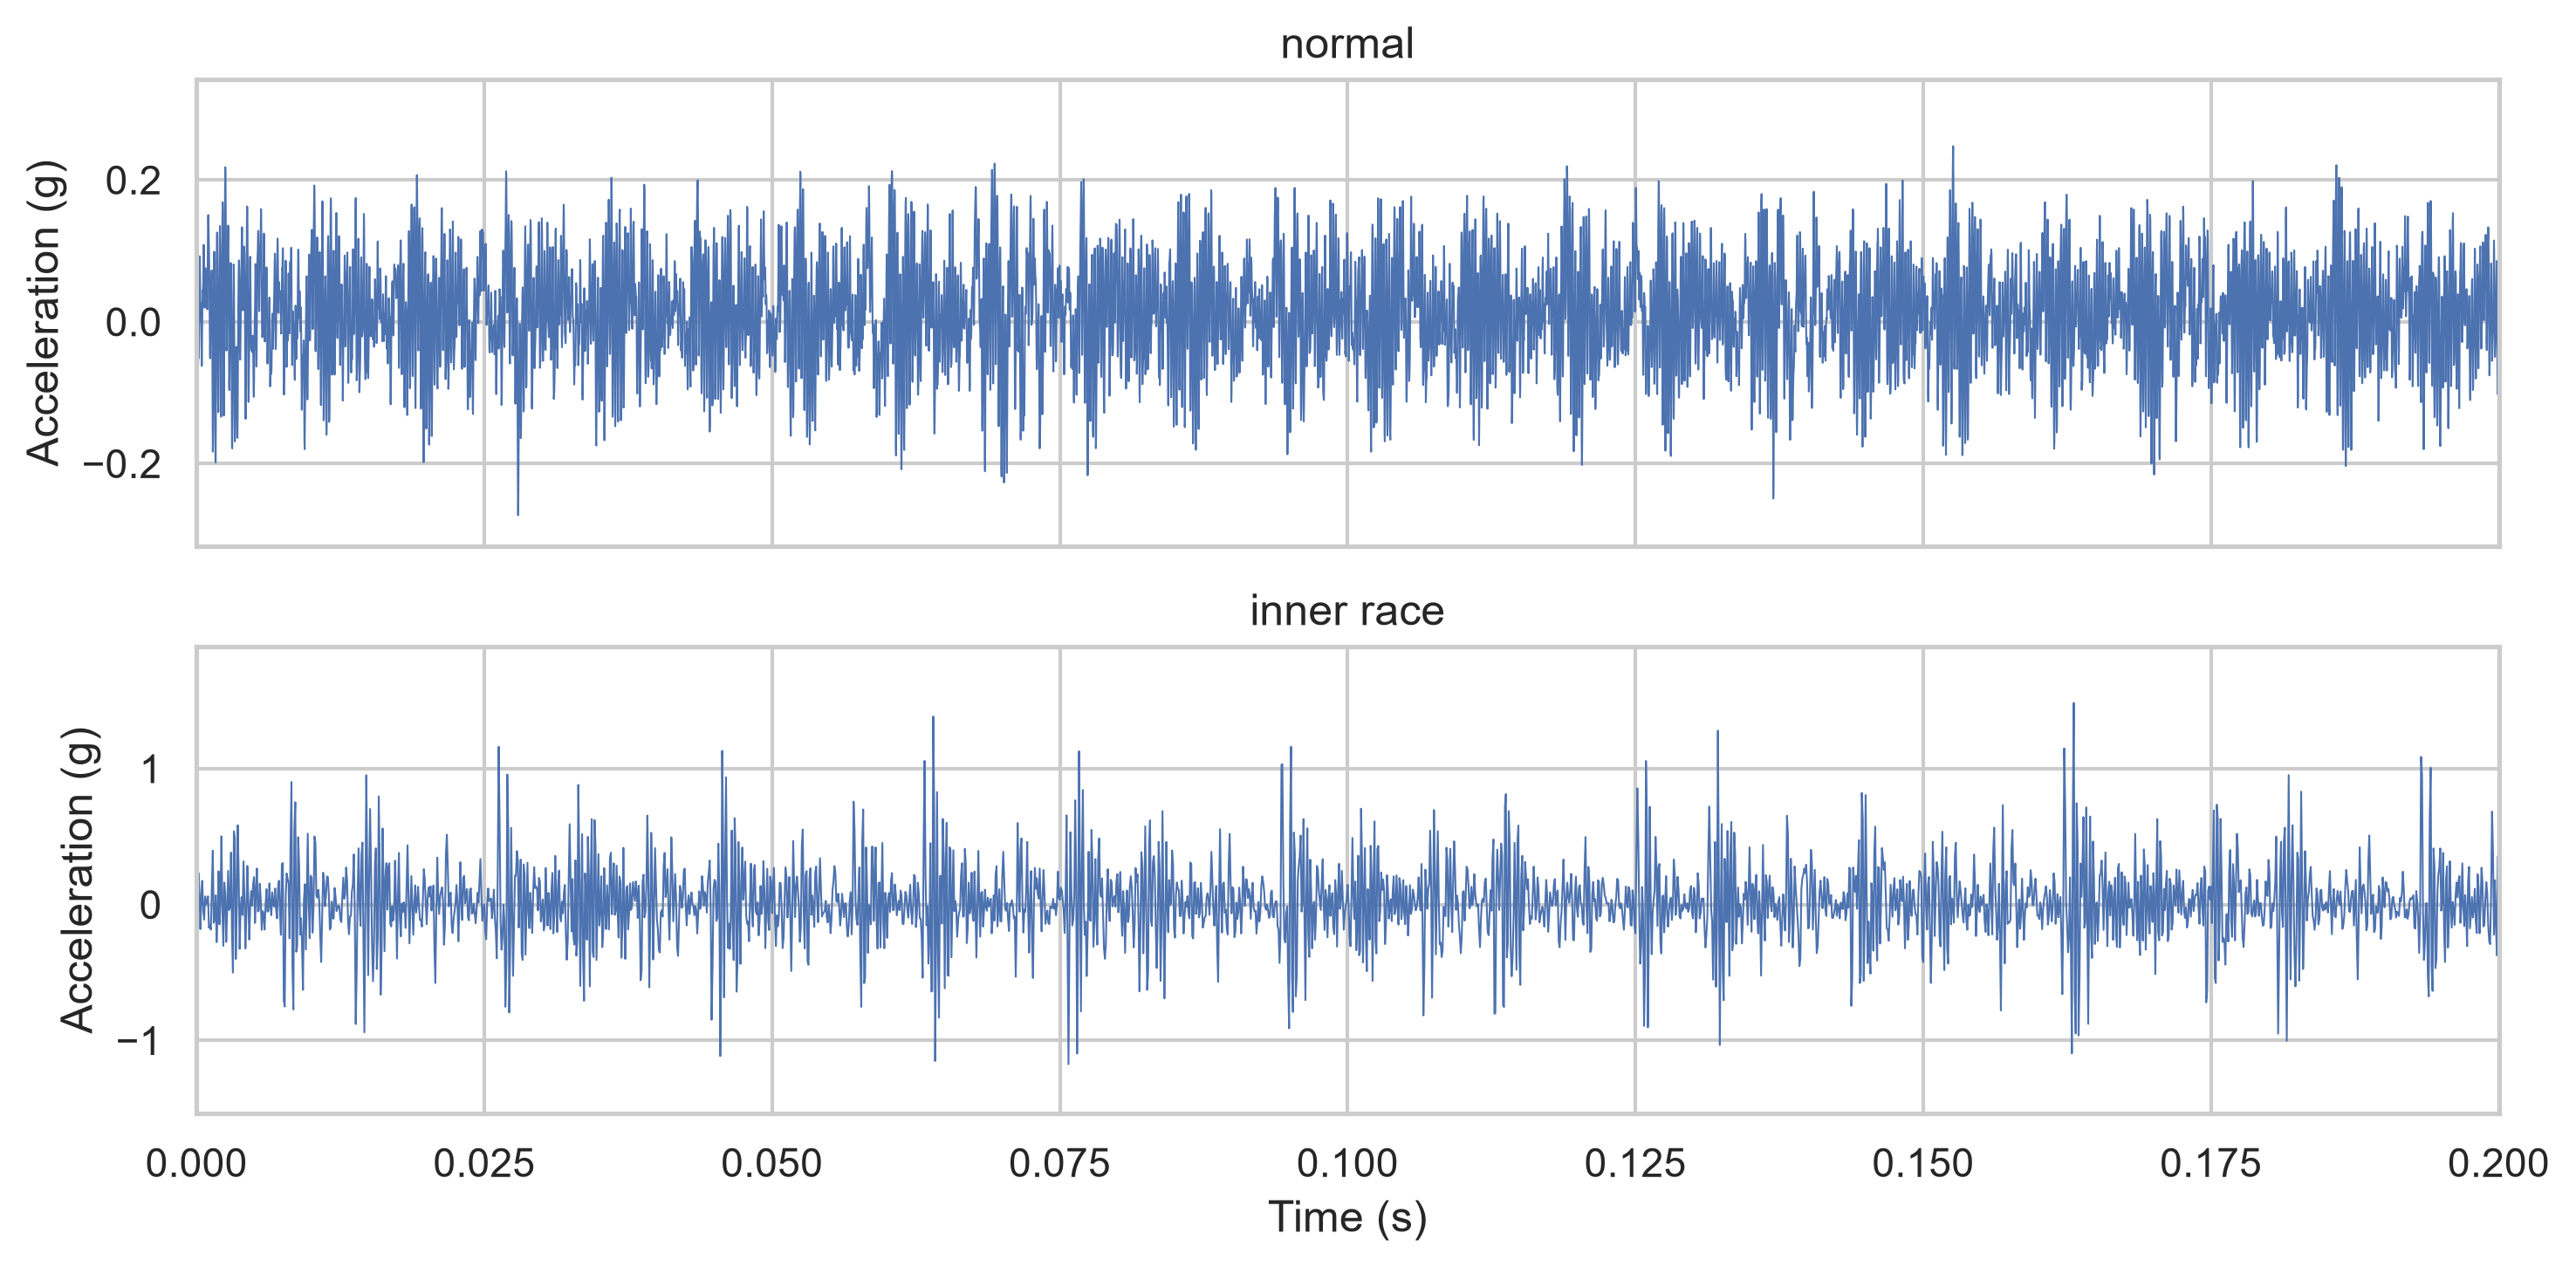
\includegraphics[keepaspectratio]{notebooks/10-signals_files/figure-pdf/cell-4-output-1.png}}

\textbf{Discussion.} Already in the time domain the faulty bearing looks
different: short, regularly spaced impacts are visible on top of the
background vibration. Count the impacts in 0.1 s -- their rate should
match the BPFI of about 5.4 × 30 Hz ≈ 162 Hz.

\section{Live coding: amplitude
spectrum}\label{live-coding-amplitude-spectrum}

\begin{Shaded}
\begin{Highlighting}[]
\NormalTok{fig, ax }\OperatorTok{=}\NormalTok{ plt.subplots(figsize}\OperatorTok{=}\NormalTok{(}\DecValTok{10}\NormalTok{, }\DecValTok{4}\NormalTok{))}
\ControlFlowTok{for}\NormalTok{ label, (x, fs) }\KeywordTok{in}\NormalTok{ signals.items():}
\NormalTok{    f }\OperatorTok{=}\NormalTok{ np.fft.rfftfreq(}\BuiltInTok{len}\NormalTok{(x), }\DecValTok{1} \OperatorTok{/}\NormalTok{ fs)}
\NormalTok{    A }\OperatorTok{=} \DecValTok{2} \OperatorTok{*}\NormalTok{ np.}\BuiltInTok{abs}\NormalTok{(np.fft.rfft(x)) }\OperatorTok{/} \BuiltInTok{len}\NormalTok{(x)}
\NormalTok{    ax.plot(f, A, label}\OperatorTok{=}\NormalTok{label, lw}\OperatorTok{=}\FloatTok{0.6}\NormalTok{)}
\NormalTok{ax.}\BuiltInTok{set}\NormalTok{(xlim}\OperatorTok{=}\NormalTok{(}\DecValTok{0}\NormalTok{, }\DecValTok{6000}\NormalTok{), xlabel}\OperatorTok{=}\StringTok{"Frequency (Hz)"}\NormalTok{, ylabel}\OperatorTok{=}\StringTok{"Amplitude (g)"}\NormalTok{,}
\NormalTok{       title}\OperatorTok{=}\StringTok{"Amplitude spectrum of the raw signals"}\NormalTok{)}
\NormalTok{ax.legend()}\OperatorTok{;}\NormalTok{ plt.show()}
\end{Highlighting}
\end{Shaded}

\pandocbounded{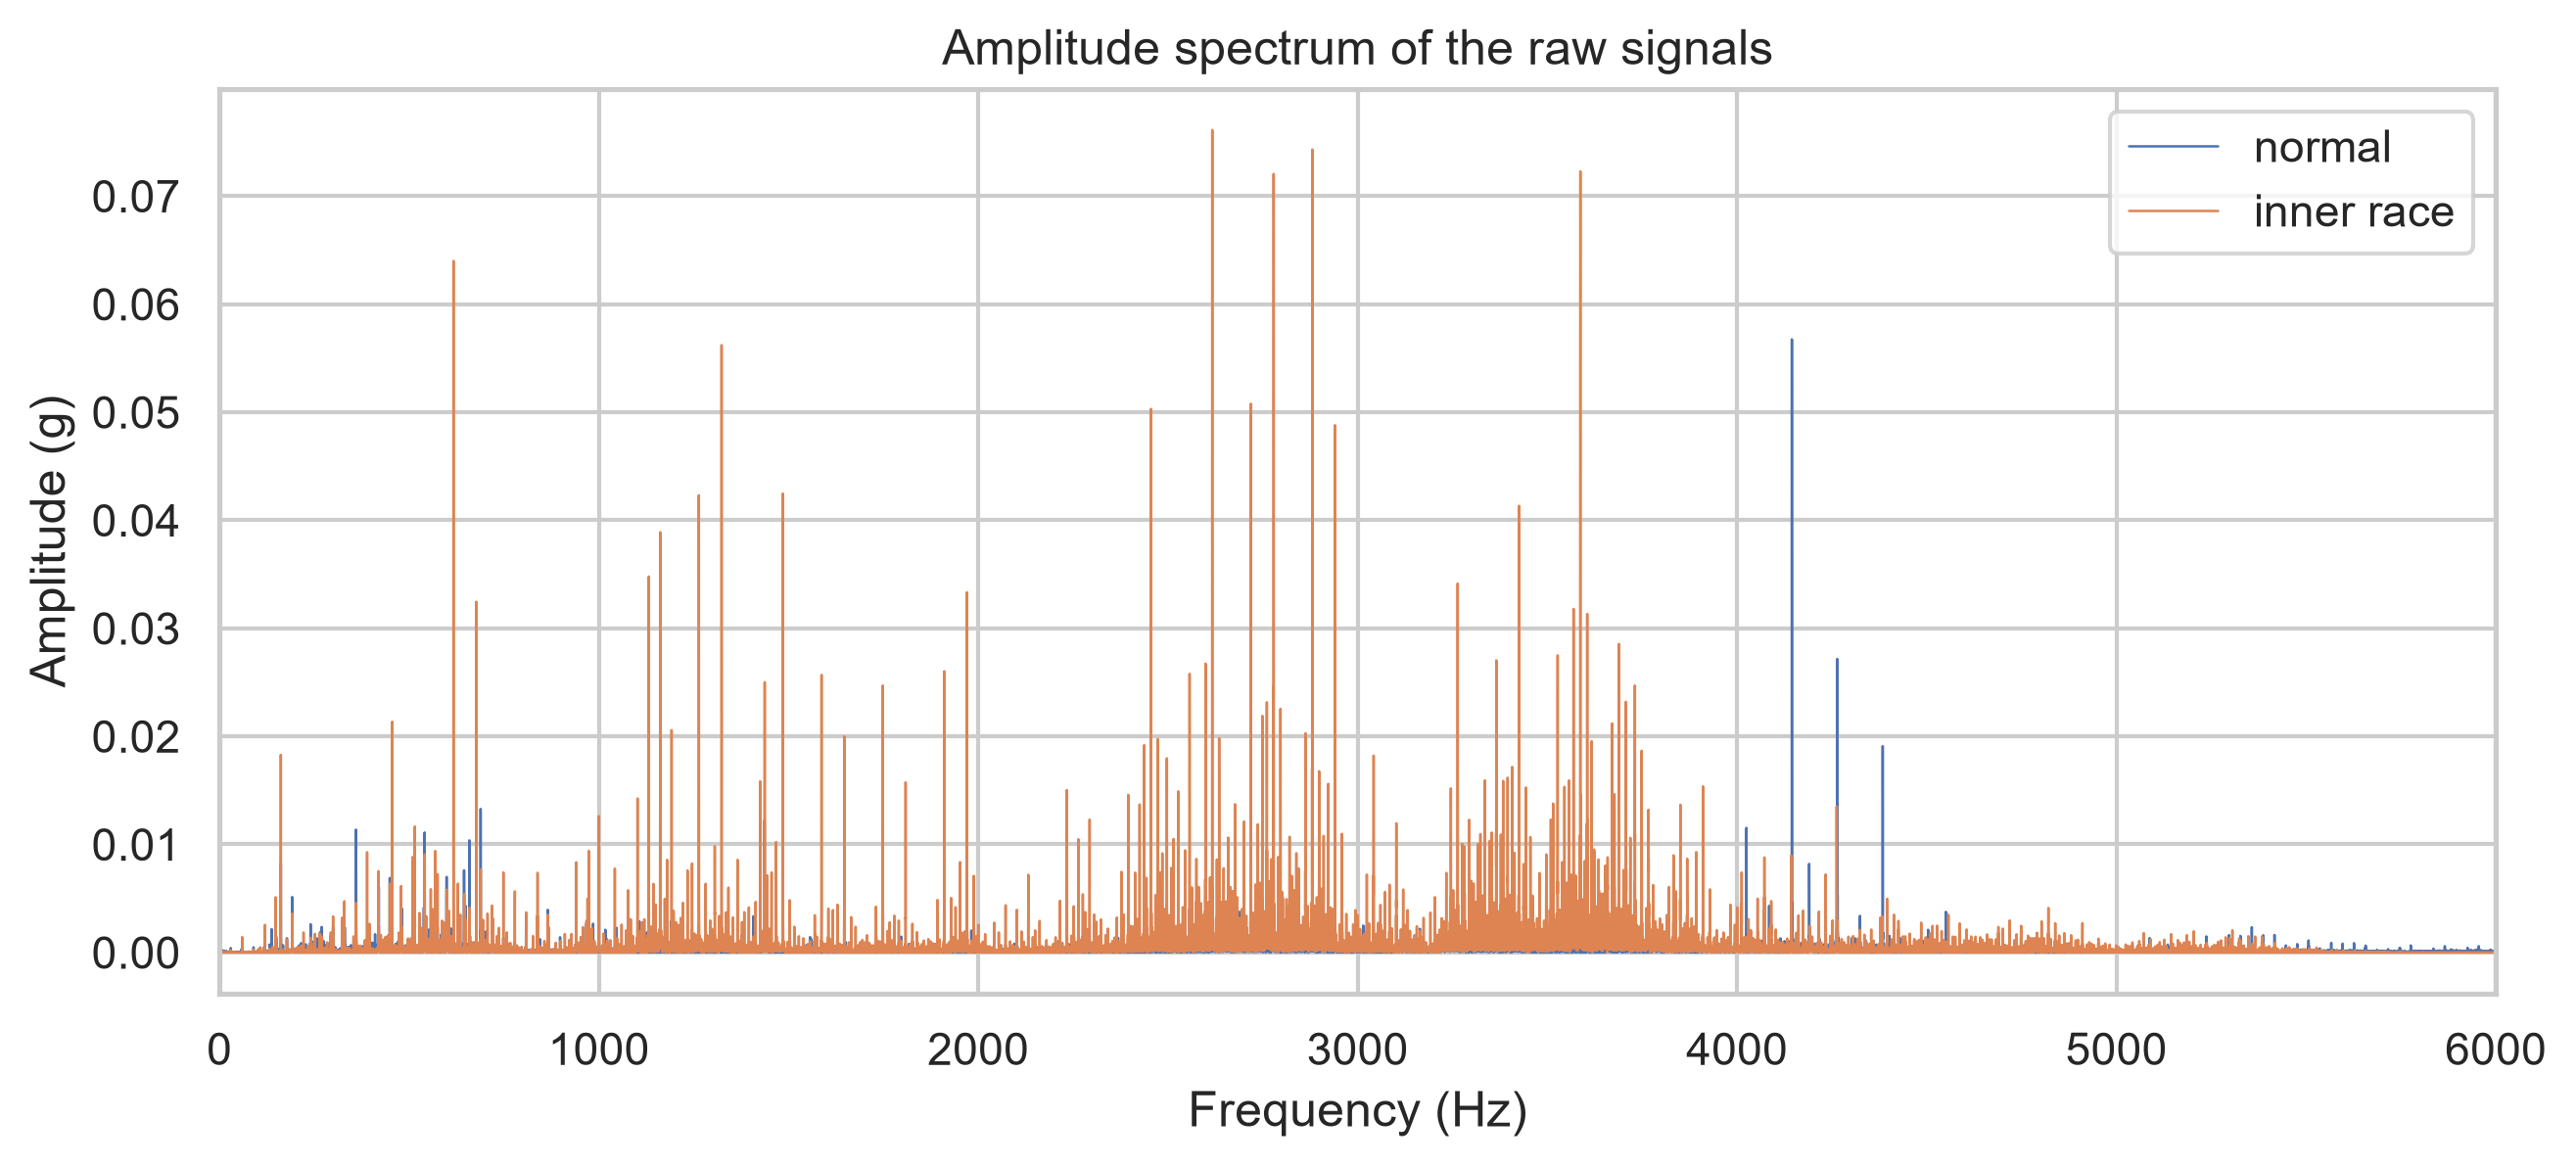
\includegraphics[keepaspectratio]{notebooks/10-signals_files/figure-pdf/cell-5-output-1.png}}

\textbf{Discussion.} The faulty bearing shows much more energy at high
frequencies, in the range of several kilohertz. These are
\textbf{structural resonances} of the bearing and housing, excited by
the impacts -- not the fault frequency itself. The impact rate of about
162 Hz modulates these resonances but is hard to see directly in this
spectrum. Envelope analysis makes it visible.

\section{Extension: envelope
analysis}\label{extension-envelope-analysis}

\emph{Extension -- optional material, not required for the exam.}

\begin{figure}[H]

\centering{

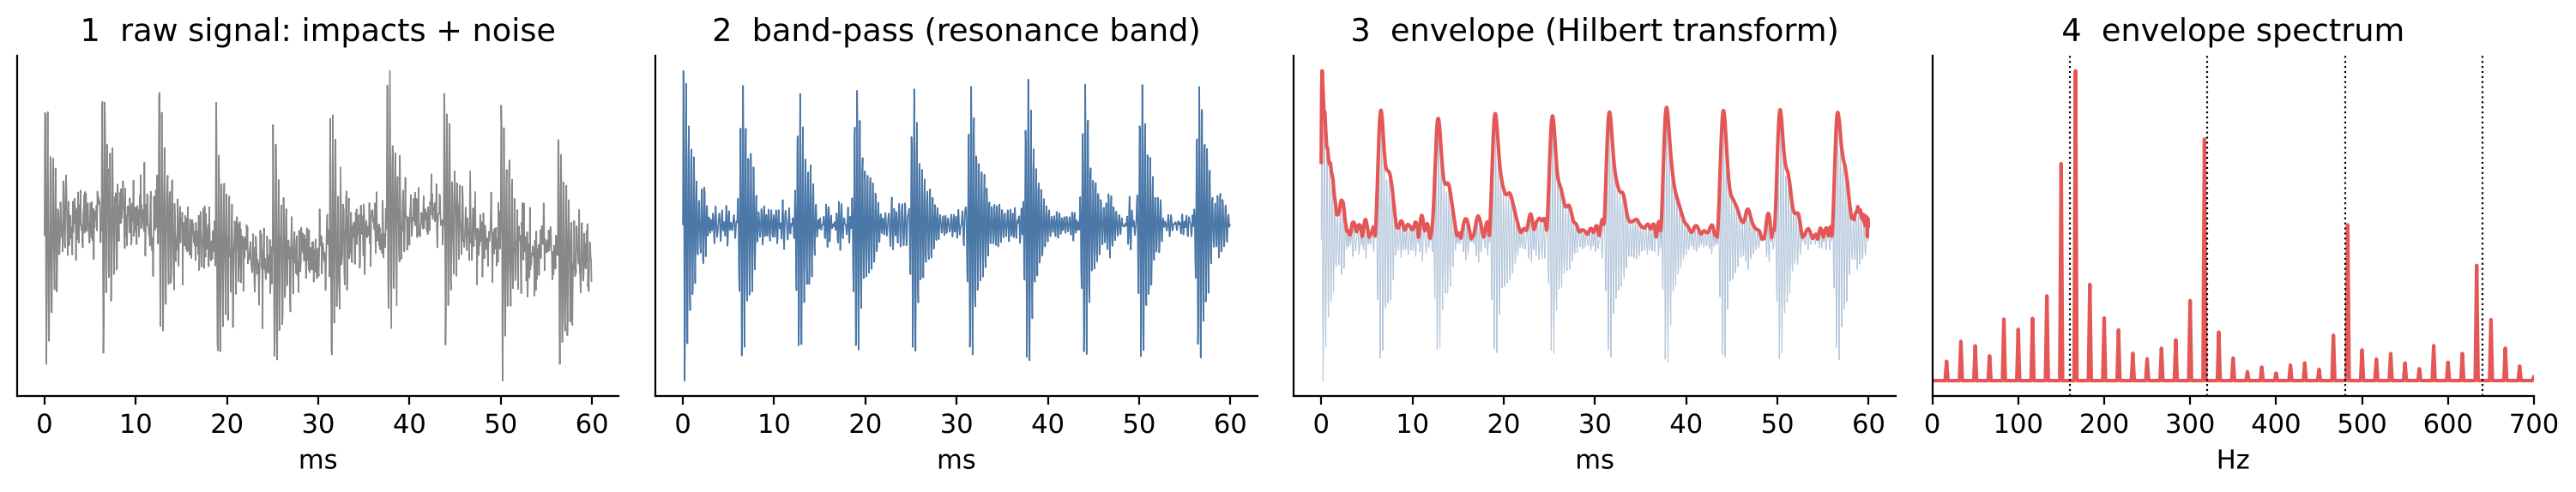
\includegraphics[width=1\linewidth,height=\textheight,keepaspectratio]{notebooks/images/envelope.png}

}

\caption{\label{fig-envelope}Envelope analysis. Periodic impacts excite
a high-frequency resonance (1). A band-pass filter isolates the
resonance band (2). The envelope -- the magnitude of the analytic signal
from the Hilbert transform -- recovers the impact pattern (3). Its
spectrum shows peaks at the impact frequency and its harmonics (4).}

\end{figure}%

The plain spectrum shows \emph{that} the faulty bearing excites
high-frequency resonances, but not \emph{why}. The envelope spectrum
reveals the repetition rate of the impacts -- and thus the damaged
component.

\begin{Shaded}
\begin{Highlighting}[]
\NormalTok{f\_r }\OperatorTok{=} \DecValTok{1797} \OperatorTok{/} \DecValTok{60}          \CommentTok{\# shaft frequency (Hz)}
\NormalTok{bpfi }\OperatorTok{=} \FloatTok{5.4152} \OperatorTok{*}\NormalTok{ f\_r}

\KeywordTok{def}\NormalTok{ envelope\_spectrum(x, fs, band}\OperatorTok{=}\NormalTok{(}\DecValTok{2000}\NormalTok{, }\DecValTok{5000}\NormalTok{)):}
\NormalTok{    b, a }\OperatorTok{=}\NormalTok{ signal.butter(}\DecValTok{4}\NormalTok{, band, btype}\OperatorTok{=}\StringTok{"bandpass"}\NormalTok{, fs}\OperatorTok{=}\NormalTok{fs)}
\NormalTok{    env }\OperatorTok{=}\NormalTok{ np.}\BuiltInTok{abs}\NormalTok{(signal.hilbert(signal.filtfilt(b, a, x)))}
\NormalTok{    env }\OperatorTok{{-}=}\NormalTok{ env.mean()}
\NormalTok{    f }\OperatorTok{=}\NormalTok{ np.fft.rfftfreq(}\BuiltInTok{len}\NormalTok{(env), }\DecValTok{1} \OperatorTok{/}\NormalTok{ fs)}
    \ControlFlowTok{return}\NormalTok{ f, np.}\BuiltInTok{abs}\NormalTok{(np.fft.rfft(env)) }\OperatorTok{/} \BuiltInTok{len}\NormalTok{(env)}

\NormalTok{fig, ax }\OperatorTok{=}\NormalTok{ plt.subplots(figsize}\OperatorTok{=}\NormalTok{(}\DecValTok{10}\NormalTok{, }\DecValTok{4}\NormalTok{))}
\ControlFlowTok{for}\NormalTok{ label, (x, fs) }\KeywordTok{in}\NormalTok{ signals.items():}
\NormalTok{    f, A }\OperatorTok{=}\NormalTok{ envelope\_spectrum(x, fs)}
\NormalTok{    ax.plot(f, A, label}\OperatorTok{=}\NormalTok{label, lw}\OperatorTok{=}\FloatTok{0.8}\NormalTok{)}
\ControlFlowTok{for}\NormalTok{ k }\KeywordTok{in}\NormalTok{ (}\DecValTok{1}\NormalTok{, }\DecValTok{2}\NormalTok{, }\DecValTok{3}\NormalTok{):}
\NormalTok{    ax.axvline(k }\OperatorTok{*}\NormalTok{ bpfi, c}\OperatorTok{=}\StringTok{"k"}\NormalTok{, ls}\OperatorTok{=}\StringTok{":"}\NormalTok{, lw}\OperatorTok{=}\DecValTok{1}\NormalTok{)}
\NormalTok{ax.}\BuiltInTok{set}\NormalTok{(xlim}\OperatorTok{=}\NormalTok{(}\DecValTok{0}\NormalTok{, }\DecValTok{600}\NormalTok{), xlabel}\OperatorTok{=}\StringTok{"Frequency (Hz)"}\NormalTok{, ylabel}\OperatorTok{=}\StringTok{"Envelope amplitude"}\NormalTok{,}
\NormalTok{       title}\OperatorTok{=}\StringTok{"Envelope spectrum, dotted: BPFI harmonics"}\NormalTok{)}
\NormalTok{ax.legend()}\OperatorTok{;}\NormalTok{ plt.show()}
\end{Highlighting}
\end{Shaded}

\pandocbounded{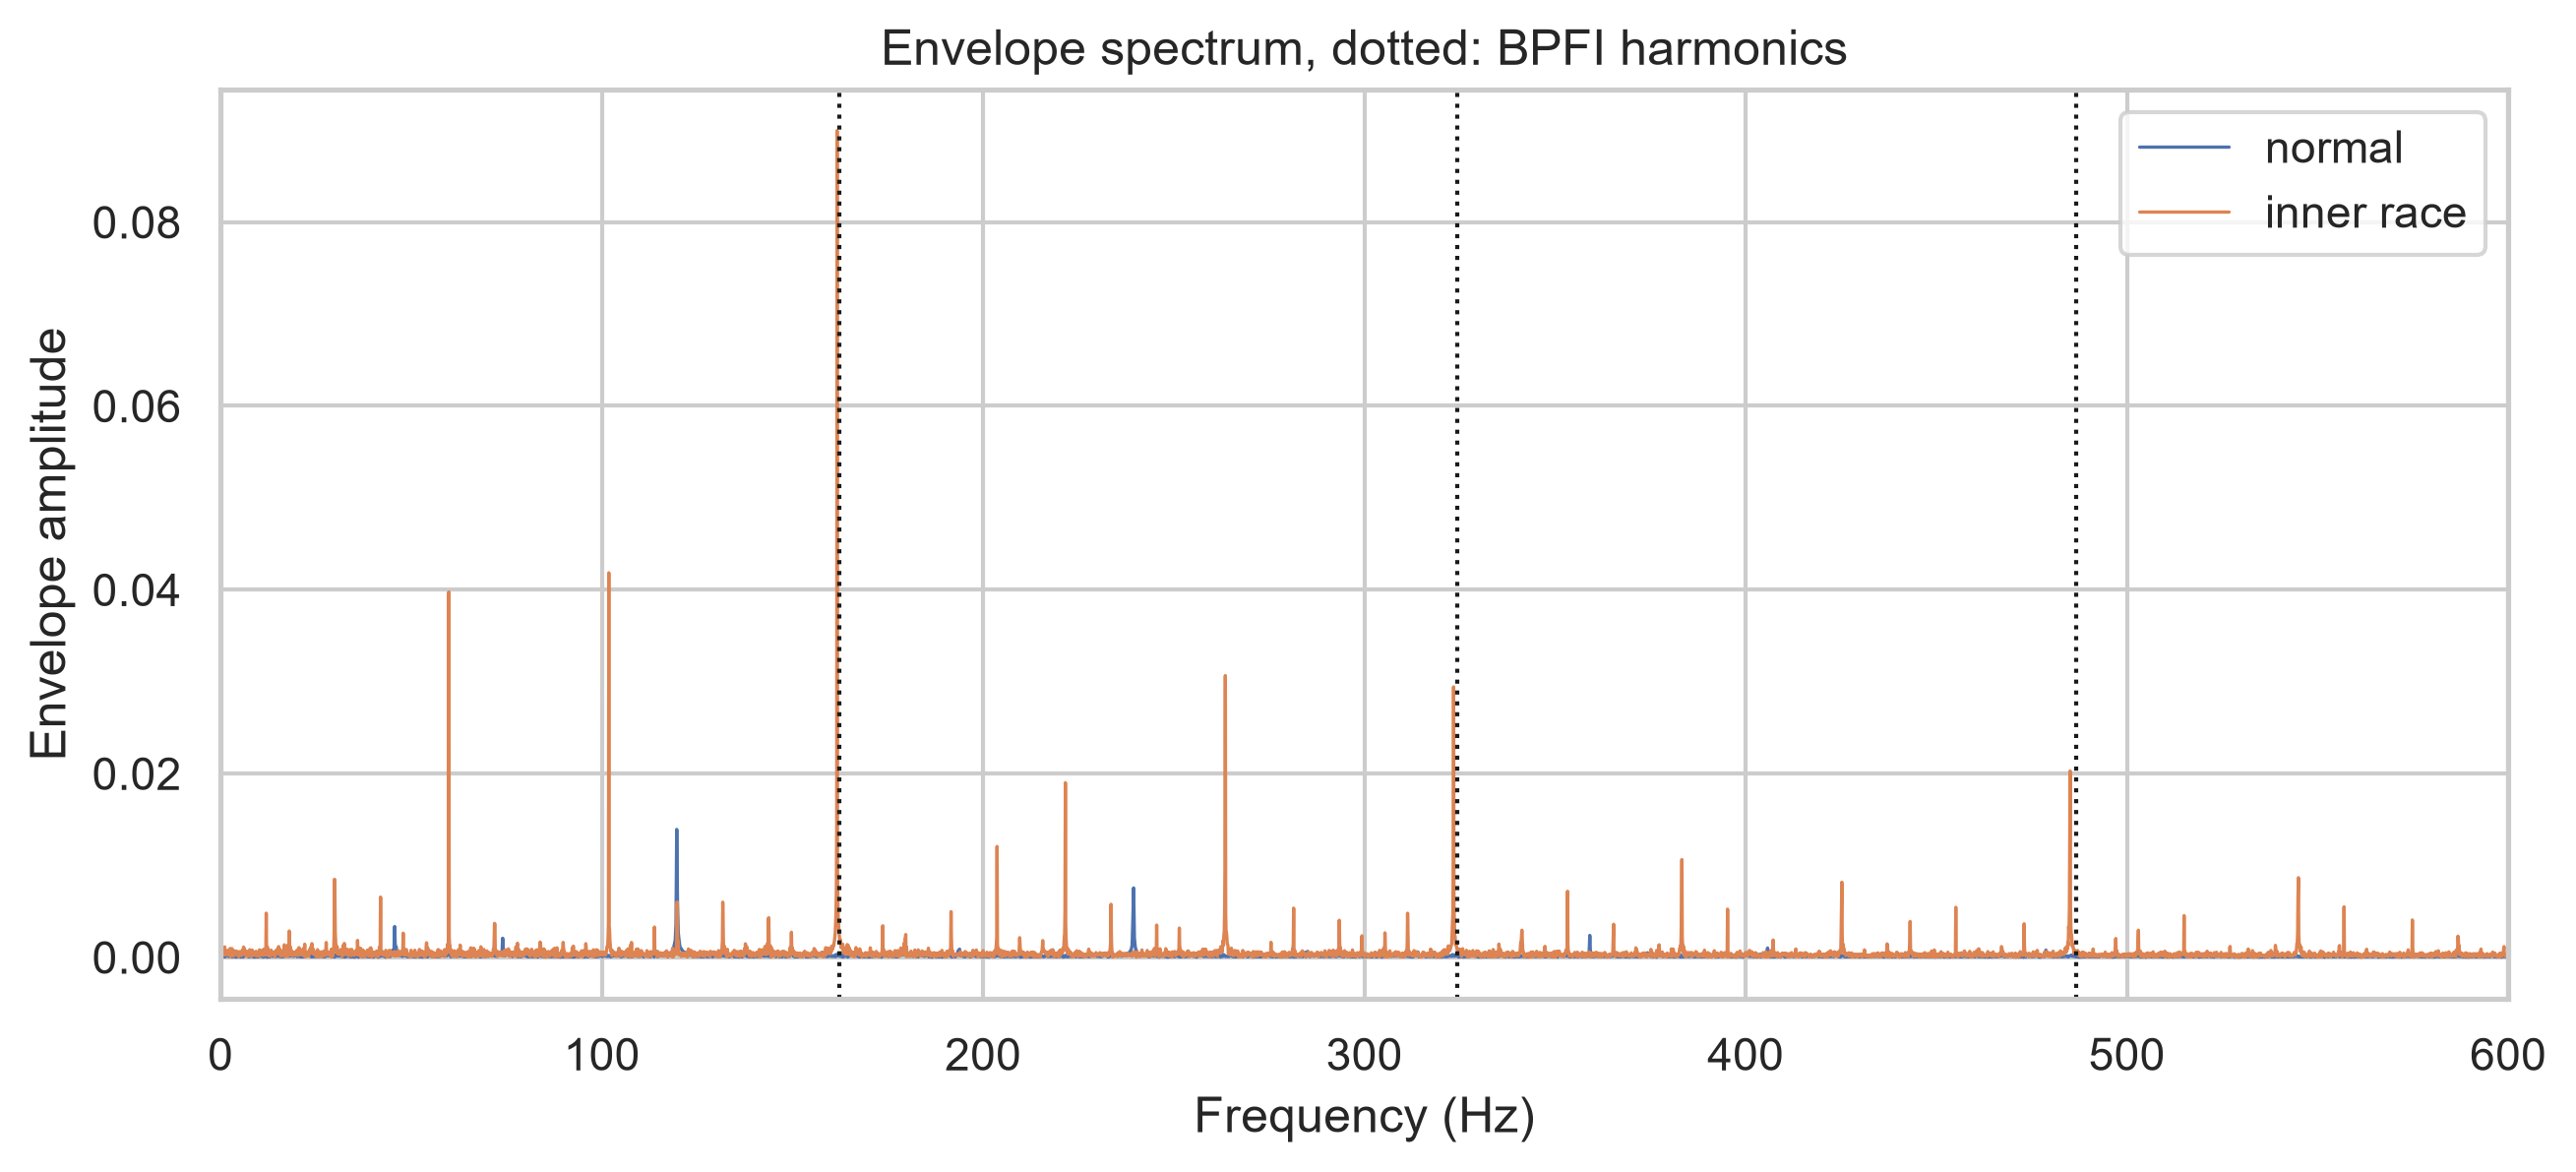
\includegraphics[keepaspectratio]{notebooks/10-signals_files/figure-pdf/cell-6-output-1.png}}

For the inner race fault, peaks appear at BPFI and its harmonics; often
there are also sidebands spaced at the shaft frequency, because the
defect on the rotating inner ring moves in and out of the load zone once
per revolution. The choice of the band (here 2--5 kHz) matters: it
should contain the resonance excited by the impacts. Methods such as the
\emph{kurtogram} select it automatically.

\section{Live coding: statistical
features}\label{live-coding-statistical-features}

\begin{Shaded}
\begin{Highlighting}[]
\KeywordTok{def}\NormalTok{ features(x):}
\NormalTok{    rms }\OperatorTok{=}\NormalTok{ np.sqrt(np.mean(x}\OperatorTok{**}\DecValTok{2}\NormalTok{))}
    \ControlFlowTok{return}\NormalTok{ \{}\StringTok{"rms"}\NormalTok{: rms, }\StringTok{"peak"}\NormalTok{: np.}\BuiltInTok{max}\NormalTok{(np.}\BuiltInTok{abs}\NormalTok{(x)), }\StringTok{"crest"}\NormalTok{: np.}\BuiltInTok{max}\NormalTok{(np.}\BuiltInTok{abs}\NormalTok{(x)) }\OperatorTok{/}\NormalTok{ rms,}
            \StringTok{"kurtosis"}\NormalTok{: stats.kurtosis(x), }\StringTok{"skewness"}\NormalTok{: stats.skew(x)\}}

\CommentTok{\# features on 1{-}second windows}
\NormalTok{rows }\OperatorTok{=}\NormalTok{ []}
\ControlFlowTok{for}\NormalTok{ label, (x, fs) }\KeywordTok{in}\NormalTok{ signals.items():}
    \ControlFlowTok{for}\NormalTok{ start }\KeywordTok{in} \BuiltInTok{range}\NormalTok{(}\DecValTok{0}\NormalTok{, }\BuiltInTok{len}\NormalTok{(x) }\OperatorTok{{-}}\NormalTok{ fs, fs):}
\NormalTok{        rows.append(\{}\StringTok{"condition"}\NormalTok{: label, }\OperatorTok{**}\NormalTok{features(x[start:start }\OperatorTok{+}\NormalTok{ fs])\})}
\NormalTok{feat }\OperatorTok{=}\NormalTok{ pd.DataFrame(rows)}
\NormalTok{feat.groupby(}\StringTok{"condition"}\NormalTok{).mean().}\BuiltInTok{round}\NormalTok{(}\DecValTok{3}\NormalTok{)}
\end{Highlighting}
\end{Shaded}

\begin{longtable}[]{@{}llllll@{}}
\toprule\noalign{}
& rms & peak & crest & kurtosis & skewness \\
condition & & & & & \\
\midrule\noalign{}
\endhead
\bottomrule\noalign{}
\endlastfoot
inner race & 0.291 & 1.601 & 5.494 & 2.397 & 0.164 \\
normal & 0.074 & 0.279 & 3.787 & -0.235 & -0.035 \\
\end{longtable}

\textbf{Discussion.} The faulty bearing has a clearly higher kurtosis
and crest factor -- the signature of impacts. Such features can feed a
classifier (Exercise 3). They are cheap to compute, which matters for
monitoring systems running on embedded hardware, and they have an
intuitive meaning that maintenance staff understand.

\section{Back to the decision}\label{back-to-the-decision-9}

A single-feature threshold works if the feature values of healthy and
faulty windows do not overlap. We check kurtosis and crest factor and,
if they separate, place the threshold in the middle of the gap.

\begin{Shaded}
\begin{Highlighting}[]
\ControlFlowTok{for}\NormalTok{ f\_name }\KeywordTok{in}\NormalTok{ [}\StringTok{"kurtosis"}\NormalTok{, }\StringTok{"crest"}\NormalTok{]:}
\NormalTok{    healthy\_max }\OperatorTok{=}\NormalTok{ feat.loc[feat.condition }\OperatorTok{==} \StringTok{"normal"}\NormalTok{, f\_name].}\BuiltInTok{max}\NormalTok{()}
\NormalTok{    faulty\_min }\OperatorTok{=}\NormalTok{ feat.loc[feat.condition }\OperatorTok{==} \StringTok{"inner race"}\NormalTok{, f\_name].}\BuiltInTok{min}\NormalTok{()}
    \ControlFlowTok{if}\NormalTok{ faulty\_min }\OperatorTok{\textgreater{}}\NormalTok{ healthy\_max:}
        \BuiltInTok{print}\NormalTok{(}\SpecialStringTok{f"}\SpecialCharTok{\{}\NormalTok{f\_name}\SpecialCharTok{:9s\}}\SpecialStringTok{: separates (healthy max }\SpecialCharTok{\{}\NormalTok{healthy\_max}\SpecialCharTok{:.2f\}}\SpecialStringTok{ \textless{} faulty min }\SpecialCharTok{\{}\NormalTok{faulty\_min}\SpecialCharTok{:.2f\}}\SpecialStringTok{) "}
              \SpecialStringTok{f"{-}\textgreater{} threshold }\SpecialCharTok{\{}\NormalTok{(healthy\_max }\OperatorTok{+}\NormalTok{ faulty\_min) }\OperatorTok{/} \DecValTok{2}\SpecialCharTok{:.2f\}}\SpecialStringTok{"}\NormalTok{)}
    \ControlFlowTok{else}\NormalTok{:}
        \BuiltInTok{print}\NormalTok{(}\SpecialStringTok{f"}\SpecialCharTok{\{}\NormalTok{f\_name}\SpecialCharTok{:9s\}}\SpecialStringTok{: overlap (healthy max }\SpecialCharTok{\{}\NormalTok{healthy\_max}\SpecialCharTok{:.2f\}}\SpecialStringTok{ \textgreater{}= faulty min }\SpecialCharTok{\{}\NormalTok{faulty\_min}\SpecialCharTok{:.2f\}}\SpecialStringTok{)"}\NormalTok{)}
\end{Highlighting}
\end{Shaded}

\begin{verbatim}
kurtosis : separates (healthy max -0.20 < faulty min 2.05) -> threshold 0.92
crest    : separates (healthy max 4.27 < faulty min 5.15) -> threshold 4.71
\end{verbatim}

If a feature separates the two recordings, the decision looks easy --
but it rests on \textbf{one} healthy and \textbf{one} faulty recording
at one load. Before ordering sensors for dozens of pumps, the threshold
must be checked on other loads, other fault types and sizes, and above
all on healthy pumps in the field, whose kurtosis can be raised by
cavitation or electrical interference. The recommendation is therefore:
a pilot on a few pumps with the chosen feature, logging the values for
some months before alarms are switched on.

\begin{tcolorbox}[enhanced jigsaw, colframe=quarto-callout-important-color-frame, toprule=.15mm, rightrule=.15mm, title=\textcolor{quarto-callout-important-color}{\faExclamation}\hspace{0.5em}{Key takeaways}, colbacktitle=quarto-callout-important-color!10!white, left=2mm, titlerule=0mm, bottomtitle=1mm, toptitle=1mm, opacityback=0, bottomrule=.15mm, breakable, arc=.35mm, opacitybacktitle=0.6, colback=white, coltitle=black, leftrule=.75mm]

\begin{itemize}
\tightlist
\item
  Sample at more than twice the highest relevant frequency and filter
  before sampling -- aliasing cannot be undone.
\item
  The FFT reveals periodic components; frequency resolution is \(1/T\),
  leakage is reduced by window functions.
\item
  Bearing geometry determines where fault frequencies appear;
  physics-based features are robust and explainable.
\item
  RMS, crest factor and kurtosis summarise signal windows; split windows
  by recording, not randomly.
\end{itemize}

\end{tcolorbox}

\section{Exercises}\label{exercises-9}

\begin{enumerate}
\def\labelenumi{\arabic{enumi}.}
\tightlist
\item
  A vibration signal contains a component at 7 kHz. It is sampled at 10
  kHz without anti-aliasing filter. At which frequency does the
  component appear in the spectrum? What sampling rate would be needed?
\item
  You record 0.5 s of vibration data at 12 kHz. What is the frequency
  resolution? Can you separate the BPFI (≈ 162.3 Hz) from its sideband
  at BPFI + \(f_r\)?
\item
  Build a classifier for normal / inner race / ball / outer race faults
  on the statistical window features. Split each recording in time
  (first 70 \% of the windows for training, last 30 \% for testing). Why
  is a random split of the windows wrong?
\item
  Hydraulic system: compute features per cycle (mean, std, max) for the
  100 Hz pressure sensors and predict the valve condition with a random
  forest. Use stratified cross-validation.
\item
  (Extension) Compare the plain amplitude spectrum with the envelope
  spectrum around BPFI. Then download an outer race fault file and check
  whether a peak appears at BPFO.
\end{enumerate}

\subsection{Solutions}\label{solutions-9}

\begin{tcolorbox}[enhanced jigsaw, colframe=quarto-callout-caution-color-frame, toprule=.15mm, rightrule=.15mm, title=\textcolor{quarto-callout-caution-color}{\faFire}\hspace{0.5em}{Solution to Exercise 1}, colbacktitle=quarto-callout-caution-color!10!white, left=2mm, titlerule=0mm, bottomtitle=1mm, toptitle=1mm, opacityback=0, bottomrule=.15mm, breakable, arc=.35mm, opacitybacktitle=0.6, colback=white, coltitle=black, leftrule=.75mm]

The Nyquist frequency is 5 kHz. The 7 kHz component is folded back to
\(|7 - 10| = 3\) kHz -- it appears as a false peak at 3 kHz. To capture
7 kHz correctly, the sampling rate must exceed 14 kHz; in practice one
chooses about 2.5 times the highest frequency of interest (≥ 17.5 kHz)
and uses an anti-aliasing filter with its cut-off below the Nyquist
frequency.

\end{tcolorbox}

\begin{tcolorbox}[enhanced jigsaw, colframe=quarto-callout-caution-color-frame, toprule=.15mm, rightrule=.15mm, title=\textcolor{quarto-callout-caution-color}{\faFire}\hspace{0.5em}{Solution to Exercise 2}, colbacktitle=quarto-callout-caution-color!10!white, left=2mm, titlerule=0mm, bottomtitle=1mm, toptitle=1mm, opacityback=0, bottomrule=.15mm, breakable, arc=.35mm, opacitybacktitle=0.6, colback=white, coltitle=black, leftrule=.75mm]

\(\Delta f = 1/T = 1/0.5\,\text{s} = 2\) Hz. The sideband lies
\(f_r \approx 30\) Hz from the BPFI peak, i.e.~15 bins away -- easily
separable. Peaks closer than about 2--3 bins (here 4--6 Hz) could not be
separated, especially with a window function that widens the peaks. Note
that the sampling rate does not affect the resolution; only the duration
does.

\end{tcolorbox}

\begin{tcolorbox}[enhanced jigsaw, colframe=quarto-callout-caution-color-frame, toprule=.15mm, rightrule=.15mm, title=\textcolor{quarto-callout-caution-color}{\faFire}\hspace{0.5em}{Solution to Exercise 3}, colbacktitle=quarto-callout-caution-color!10!white, left=2mm, titlerule=0mm, bottomtitle=1mm, toptitle=1mm, opacityback=0, bottomrule=.15mm, breakable, arc=.35mm, opacitybacktitle=0.6, colback=white, coltitle=black, leftrule=.75mm]

\begin{Shaded}
\begin{Highlighting}[]
\ImportTok{from}\NormalTok{ sklearn.ensemble }\ImportTok{import}\NormalTok{ RandomForestClassifier}
\ImportTok{from}\NormalTok{ sklearn.metrics }\ImportTok{import}\NormalTok{ classification\_report}

\NormalTok{FILES4 }\OperatorTok{=}\NormalTok{ \{}\StringTok{"normal"}\NormalTok{: (}\StringTok{"97.mat"}\NormalTok{, }\DecValTok{48\_000}\NormalTok{), }\StringTok{"inner race"}\NormalTok{: (}\StringTok{"105.mat"}\NormalTok{, }\DecValTok{12\_000}\NormalTok{),}
          \StringTok{"ball"}\NormalTok{: (}\StringTok{"118.mat"}\NormalTok{, }\DecValTok{12\_000}\NormalTok{), }\StringTok{"outer race"}\NormalTok{: (}\StringTok{"130.mat"}\NormalTok{, }\DecValTok{12\_000}\NormalTok{)\}   }\CommentTok{\# verify on the CWRU pages!}
\NormalTok{rows }\OperatorTok{=}\NormalTok{ []}
\ControlFlowTok{for}\NormalTok{ label, (fname, fs) }\KeywordTok{in}\NormalTok{ FILES4.items():}
\NormalTok{    mat }\OperatorTok{=}\NormalTok{ loadmat(download(BASE\_URL }\OperatorTok{+}\NormalTok{ fname))}
\NormalTok{    x }\OperatorTok{=}\NormalTok{ mat[}\BuiltInTok{next}\NormalTok{(k }\ControlFlowTok{for}\NormalTok{ k }\KeywordTok{in}\NormalTok{ mat }\ControlFlowTok{if}\NormalTok{ k.endswith(}\StringTok{"\_DE\_time"}\NormalTok{))].ravel()}
    \ControlFlowTok{if}\NormalTok{ fs }\OperatorTok{==} \DecValTok{48\_000}\NormalTok{:                                   }\CommentTok{\# bring all signals to 12 kHz}
\NormalTok{        x, fs }\OperatorTok{=}\NormalTok{ signal.decimate(x, }\DecValTok{4}\NormalTok{), }\DecValTok{12\_000}
\NormalTok{    win }\OperatorTok{=}\NormalTok{ fs }\OperatorTok{//} \DecValTok{4}                                      \CommentTok{\# 0.25 s windows}
\NormalTok{    starts }\OperatorTok{=} \BuiltInTok{range}\NormalTok{(}\DecValTok{0}\NormalTok{, }\BuiltInTok{len}\NormalTok{(x) }\OperatorTok{{-}}\NormalTok{ win, win)}
\NormalTok{    n\_train }\OperatorTok{=} \BuiltInTok{int}\NormalTok{(}\FloatTok{0.7} \OperatorTok{*} \BuiltInTok{len}\NormalTok{(starts))}
    \ControlFlowTok{for}\NormalTok{ i, s }\KeywordTok{in} \BuiltInTok{enumerate}\NormalTok{(starts):}
\NormalTok{        rows.append(\{}\StringTok{"condition"}\NormalTok{: label, }\StringTok{"train"}\NormalTok{: i }\OperatorTok{\textless{}}\NormalTok{ n\_train, }\OperatorTok{**}\NormalTok{features(x[s:s }\OperatorTok{+}\NormalTok{ win])\})}
\NormalTok{fw }\OperatorTok{=}\NormalTok{ pd.DataFrame(rows)}
\NormalTok{feat\_cols }\OperatorTok{=}\NormalTok{ [}\StringTok{"rms"}\NormalTok{, }\StringTok{"peak"}\NormalTok{, }\StringTok{"crest"}\NormalTok{, }\StringTok{"kurtosis"}\NormalTok{, }\StringTok{"skewness"}\NormalTok{]}
\NormalTok{clf }\OperatorTok{=}\NormalTok{ RandomForestClassifier(}\DecValTok{300}\NormalTok{, random\_state}\OperatorTok{=}\DecValTok{0}\NormalTok{).fit(fw.loc[fw.train, feat\_cols], fw.loc[fw.train, }\StringTok{"condition"}\NormalTok{])}
\BuiltInTok{print}\NormalTok{(classification\_report(fw.loc[}\OperatorTok{\textasciitilde{}}\NormalTok{fw.train, }\StringTok{"condition"}\NormalTok{], clf.predict(fw.loc[}\OperatorTok{\textasciitilde{}}\NormalTok{fw.train, feat\_cols])))}
\end{Highlighting}
\end{Shaded}

\begin{verbatim}
              precision    recall  f1-score   support

        ball       1.00      1.00      1.00        12
  inner race       1.00      1.00      1.00        12
      normal       1.00      1.00      1.00         6
  outer race       1.00      1.00      1.00        12

    accuracy                           1.00        42
   macro avg       1.00      1.00      1.00        42
weighted avg       1.00      1.00      1.00        42
\end{verbatim}

All signals are first brought to the same sampling rate, because
features such as peak and RMS depend on the bandwidth. A random split
would put neighbouring, nearly identical windows into training and test,
so the test accuracy would measure memorisation. The time split is
better, but still optimistic: there is only one recording per condition,
so the model may learn properties of the individual test run (sensor
mounting, load) rather than the fault. A convincing evaluation needs
several recordings per class -- e.g.~train on 0 and 1 hp, test on 2 and
3 hp.

\end{tcolorbox}

\begin{tcolorbox}[enhanced jigsaw, colframe=quarto-callout-caution-color-frame, toprule=.15mm, rightrule=.15mm, title=\textcolor{quarto-callout-caution-color}{\faFire}\hspace{0.5em}{Solution to Exercise 4}, colbacktitle=quarto-callout-caution-color!10!white, left=2mm, titlerule=0mm, bottomtitle=1mm, toptitle=1mm, opacityback=0, bottomrule=.15mm, breakable, arc=.35mm, opacitybacktitle=0.6, colback=white, coltitle=black, leftrule=.75mm]

\begin{Shaded}
\begin{Highlighting}[]
\ImportTok{import}\NormalTok{ zipfile}
\ImportTok{from}\NormalTok{ sklearn.model\_selection }\ImportTok{import}\NormalTok{ cross\_val\_score, StratifiedKFold}

\NormalTok{hz }\OperatorTok{=}\NormalTok{ download(}\StringTok{"https://archive.ics.uci.edu/static/public/447/condition+monitoring+of+hydraulic+systems.zip"}\NormalTok{,}
              \StringTok{"hydraulic.zip"}\NormalTok{)}

\KeywordTok{def}\NormalTok{ read\_sensor(z, name):}
\NormalTok{    member }\OperatorTok{=} \BuiltInTok{next}\NormalTok{(n }\ControlFlowTok{for}\NormalTok{ n }\KeywordTok{in}\NormalTok{ z.namelist() }\ControlFlowTok{if}\NormalTok{ n.endswith(name))}
    \ControlFlowTok{return}\NormalTok{ pd.read\_csv(z.}\BuiltInTok{open}\NormalTok{(member), sep}\OperatorTok{=}\StringTok{"}\CharTok{\textbackslash{}t}\StringTok{"}\NormalTok{, header}\OperatorTok{=}\VariableTok{None}\NormalTok{).values}

\ControlFlowTok{with}\NormalTok{ zipfile.ZipFile(hz) }\ImportTok{as}\NormalTok{ z:}
\NormalTok{    ps }\OperatorTok{=}\NormalTok{ \{s: read\_sensor(z, }\SpecialStringTok{f"}\SpecialCharTok{\{}\NormalTok{s}\SpecialCharTok{\}}\SpecialStringTok{.txt"}\NormalTok{) }\ControlFlowTok{for}\NormalTok{ s }\KeywordTok{in}\NormalTok{ [}\StringTok{"PS1"}\NormalTok{, }\StringTok{"PS2"}\NormalTok{, }\StringTok{"PS3"}\NormalTok{, }\StringTok{"PS4"}\NormalTok{, }\StringTok{"PS5"}\NormalTok{, }\StringTok{"PS6"}\NormalTok{]\}}
\NormalTok{    profile }\OperatorTok{=}\NormalTok{ pd.DataFrame(read\_sensor(z, }\StringTok{"profile.txt"}\NormalTok{),}
\NormalTok{                           columns}\OperatorTok{=}\NormalTok{[}\StringTok{"cooler"}\NormalTok{, }\StringTok{"valve"}\NormalTok{, }\StringTok{"pump\_leak"}\NormalTok{, }\StringTok{"accumulator"}\NormalTok{, }\StringTok{"stable"}\NormalTok{])}
\NormalTok{feat\_ps }\OperatorTok{=}\NormalTok{ pd.DataFrame(\{}\SpecialStringTok{f"}\SpecialCharTok{\{}\NormalTok{s}\SpecialCharTok{\}}\SpecialStringTok{\_}\SpecialCharTok{\{}\NormalTok{stat}\SpecialCharTok{\}}\SpecialStringTok{"}\NormalTok{: }\BuiltInTok{getattr}\NormalTok{(np, stat)(v, axis}\OperatorTok{=}\DecValTok{1}\NormalTok{)}
                        \ControlFlowTok{for}\NormalTok{ s, v }\KeywordTok{in}\NormalTok{ ps.items() }\ControlFlowTok{for}\NormalTok{ stat }\KeywordTok{in}\NormalTok{ [}\StringTok{"mean"}\NormalTok{, }\StringTok{"std"}\NormalTok{, }\StringTok{"max"}\NormalTok{]\})}
\NormalTok{acc }\OperatorTok{=}\NormalTok{ cross\_val\_score(RandomForestClassifier(}\DecValTok{300}\NormalTok{, random\_state}\OperatorTok{=}\DecValTok{0}\NormalTok{), feat\_ps, profile[}\StringTok{"valve"}\NormalTok{].astype(}\BuiltInTok{int}\NormalTok{),}
\NormalTok{                      cv}\OperatorTok{=}\NormalTok{StratifiedKFold(}\DecValTok{5}\NormalTok{, shuffle}\OperatorTok{=}\VariableTok{True}\NormalTok{, random\_state}\OperatorTok{=}\DecValTok{0}\NormalTok{))}
\BuiltInTok{print}\NormalTok{(}\SpecialStringTok{f"Valve condition accuracy: }\SpecialCharTok{\{}\NormalTok{acc}\SpecialCharTok{.}\NormalTok{mean()}\SpecialCharTok{:.3f\}}\SpecialStringTok{ ± }\SpecialCharTok{\{}\NormalTok{acc}\SpecialCharTok{.}\NormalTok{std()}\SpecialCharTok{:.3f\}}\SpecialStringTok{"}\NormalTok{)}
\end{Highlighting}
\end{Shaded}

\begin{verbatim}
Valve condition accuracy: 0.987 ± 0.008
\end{verbatim}

Simple pressure statistics per cycle usually predict the valve condition
well, because a degraded valve changes the switching behaviour and thus
the pressure curves. Caution: the conditions were changed in blocks over
the duration of the experiment, so neighbouring cycles share conditions
\emph{and} drifting factors such as oil temperature. A time-based split
would give a more conservative estimate than the shuffled
cross-validation used here.

\end{tcolorbox}

\begin{tcolorbox}[enhanced jigsaw, colframe=quarto-callout-caution-color-frame, toprule=.15mm, rightrule=.15mm, title=\textcolor{quarto-callout-caution-color}{\faFire}\hspace{0.5em}{Solution to Exercise 5}, colbacktitle=quarto-callout-caution-color!10!white, left=2mm, titlerule=0mm, bottomtitle=1mm, toptitle=1mm, opacityback=0, bottomrule=.15mm, breakable, arc=.35mm, opacitybacktitle=0.6, colback=white, coltitle=black, leftrule=.75mm]

\begin{Shaded}
\begin{Highlighting}[]
\NormalTok{x\_ir, fs\_ir }\OperatorTok{=}\NormalTok{ signals[}\StringTok{"inner race"}\NormalTok{]}
\NormalTok{f\_plain }\OperatorTok{=}\NormalTok{ np.fft.rfftfreq(}\BuiltInTok{len}\NormalTok{(x\_ir), }\DecValTok{1} \OperatorTok{/}\NormalTok{ fs\_ir)}
\NormalTok{A\_plain }\OperatorTok{=} \DecValTok{2} \OperatorTok{*}\NormalTok{ np.}\BuiltInTok{abs}\NormalTok{(np.fft.rfft(x\_ir)) }\OperatorTok{/} \BuiltInTok{len}\NormalTok{(x\_ir)}
\NormalTok{f\_env, A\_env }\OperatorTok{=}\NormalTok{ envelope\_spectrum(x\_ir, fs\_ir)}
\NormalTok{fig, axes }\OperatorTok{=}\NormalTok{ plt.subplots(}\DecValTok{1}\NormalTok{, }\DecValTok{2}\NormalTok{, figsize}\OperatorTok{=}\NormalTok{(}\DecValTok{12}\NormalTok{, }\DecValTok{4}\NormalTok{))}
\NormalTok{axes[}\DecValTok{0}\NormalTok{].plot(f\_plain, A\_plain)}\OperatorTok{;}\NormalTok{ axes[}\DecValTok{0}\NormalTok{].}\BuiltInTok{set}\NormalTok{(xlim}\OperatorTok{=}\NormalTok{(}\DecValTok{0}\NormalTok{, }\DecValTok{600}\NormalTok{), title}\OperatorTok{=}\StringTok{"Plain spectrum"}\NormalTok{, xlabel}\OperatorTok{=}\StringTok{"Hz"}\NormalTok{)}
\NormalTok{axes[}\DecValTok{1}\NormalTok{].plot(f\_env, A\_env)}\OperatorTok{;}\NormalTok{ axes[}\DecValTok{1}\NormalTok{].}\BuiltInTok{set}\NormalTok{(xlim}\OperatorTok{=}\NormalTok{(}\DecValTok{0}\NormalTok{, }\DecValTok{600}\NormalTok{), title}\OperatorTok{=}\StringTok{"Envelope spectrum"}\NormalTok{, xlabel}\OperatorTok{=}\StringTok{"Hz"}\NormalTok{)}
\ControlFlowTok{for}\NormalTok{ ax }\KeywordTok{in}\NormalTok{ axes:}
\NormalTok{    ax.axvline(bpfi, c}\OperatorTok{=}\StringTok{"k"}\NormalTok{, ls}\OperatorTok{=}\StringTok{":"}\NormalTok{)}
\NormalTok{plt.tight\_layout()}\OperatorTok{;}\NormalTok{ plt.show()}

\NormalTok{mat }\OperatorTok{=}\NormalTok{ loadmat(download(BASE\_URL }\OperatorTok{+} \StringTok{"130.mat"}\NormalTok{))                 }\CommentTok{\# outer race fault (verify!)}
\NormalTok{x\_or }\OperatorTok{=}\NormalTok{ mat[}\BuiltInTok{next}\NormalTok{(k }\ControlFlowTok{for}\NormalTok{ k }\KeywordTok{in}\NormalTok{ mat }\ControlFlowTok{if}\NormalTok{ k.endswith(}\StringTok{"\_DE\_time"}\NormalTok{))].ravel()}
\NormalTok{f\_o, A\_o }\OperatorTok{=}\NormalTok{ envelope\_spectrum(x\_or, }\DecValTok{12\_000}\NormalTok{)}
\NormalTok{bpfo }\OperatorTok{=} \FloatTok{3.5848} \OperatorTok{*}\NormalTok{ f\_r}
\NormalTok{plt.plot(f\_o, A\_o)}\OperatorTok{;}\NormalTok{ plt.xlim(}\DecValTok{0}\NormalTok{, }\DecValTok{600}\NormalTok{)}
\ControlFlowTok{for}\NormalTok{ k }\KeywordTok{in}\NormalTok{ (}\DecValTok{1}\NormalTok{, }\DecValTok{2}\NormalTok{, }\DecValTok{3}\NormalTok{):}
\NormalTok{    plt.axvline(k }\OperatorTok{*}\NormalTok{ bpfo, c}\OperatorTok{=}\StringTok{"k"}\NormalTok{, ls}\OperatorTok{=}\StringTok{":"}\NormalTok{)}
\NormalTok{plt.title(}\StringTok{"Outer race fault: envelope spectrum, dotted: BPFO harmonics"}\NormalTok{)}\OperatorTok{;}\NormalTok{ plt.xlabel(}\StringTok{"Hz"}\NormalTok{)}
\NormalTok{plt.show()}
\end{Highlighting}
\end{Shaded}

\pandocbounded{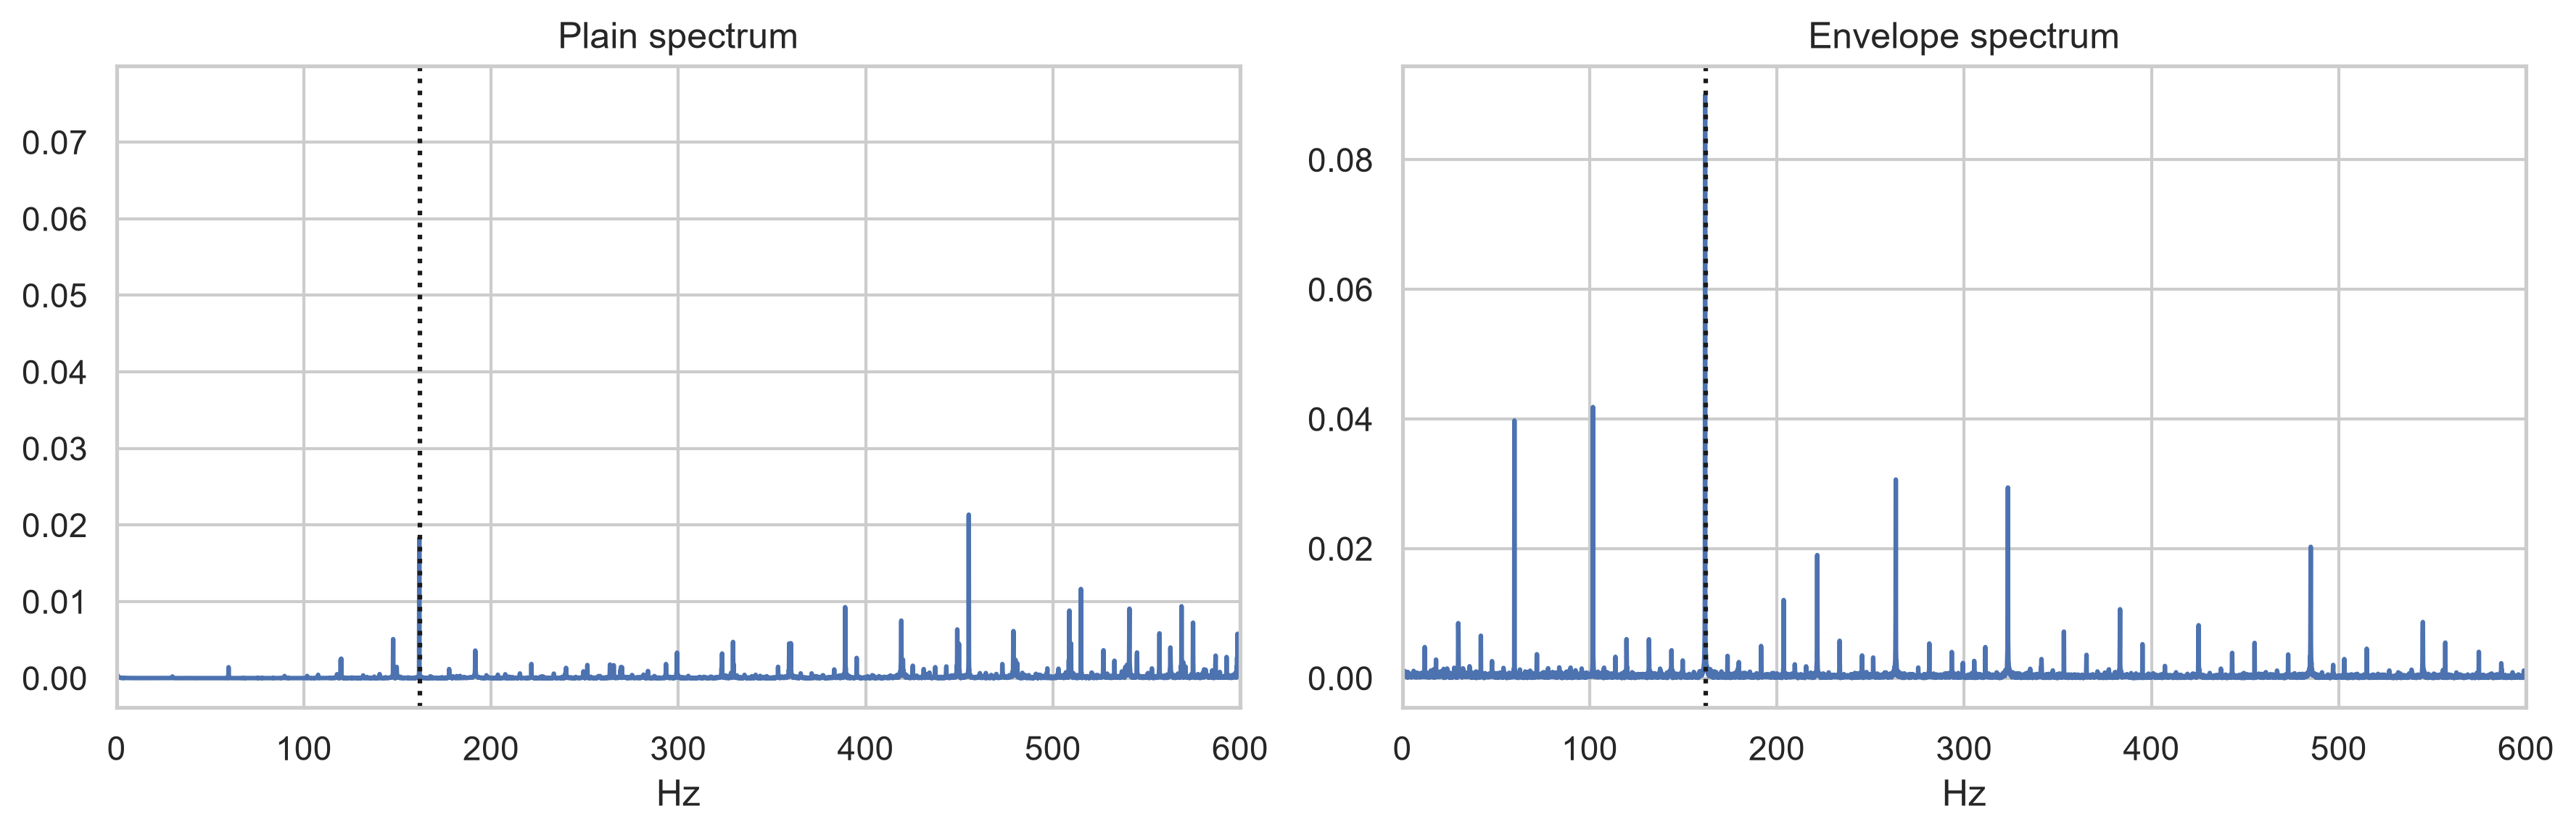
\includegraphics[keepaspectratio]{notebooks/10-signals_files/figure-pdf/cell-11-output-1.png}}

\pandocbounded{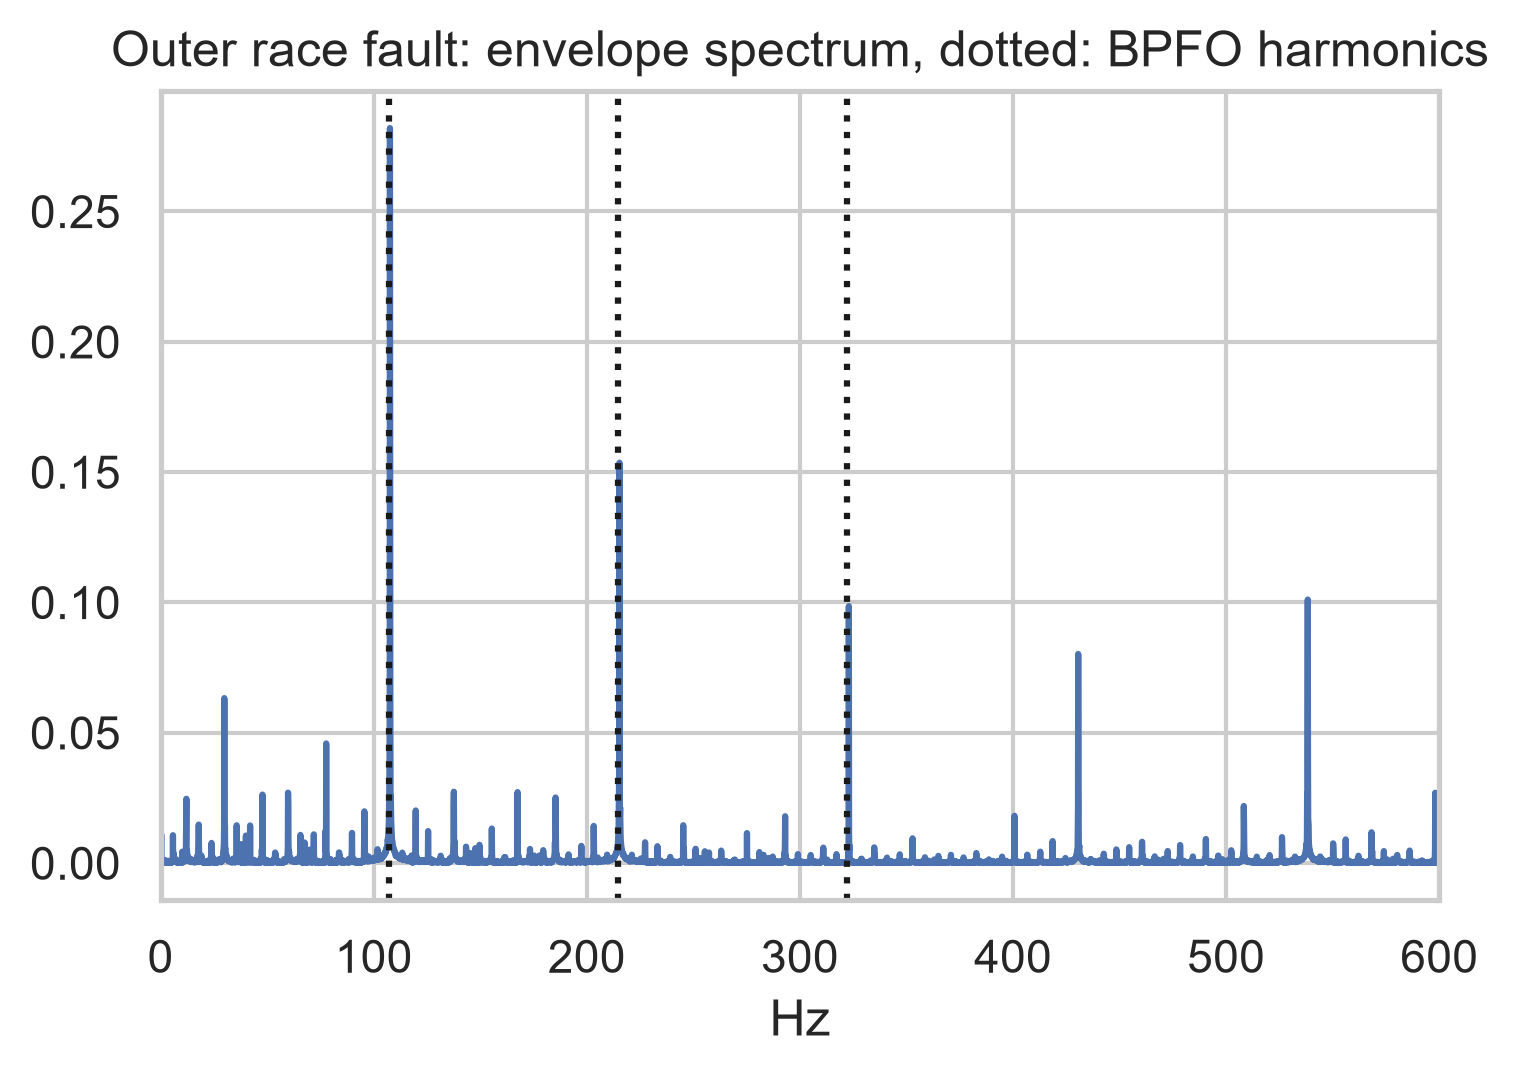
\includegraphics[keepaspectratio]{notebooks/10-signals_files/figure-pdf/cell-11-output-2.png}}

In the plain spectrum, the low-frequency range is dominated by shaft
harmonics and noise, and the impact rate hardly shows, because the
impacts carry their energy at the resonance frequencies. The envelope
spectrum demodulates the resonance and reveals BPFI clearly. For the
outer race fault, the peaks appear at BPFO; since the outer ring is
stationary, the defect stays in the same position relative to the load
zone, and shaft-frequency sidebands are typically weaker than for inner
race faults.

\end{tcolorbox}

\part{Part D -- Time Series, Deep Learning and Review}

\chapter{Time Series Forecasting}\label{time-series-forecasting}

Grid operators must know tomorrow's electricity demand to schedule power
plants; a factory plans shifts based on forecast orders; an energy
manager wants to know the peak load of next week. All of these are
\textbf{forecasting} problems on time series -- sequences of
measurements ordered in time.

Time series differ from the tabular data of the previous chapters in one
fundamental way: the observations are not independent. Today's load is
strongly related to yesterday's and to the load one week ago. This
dependence is what makes forecasting possible -- and it changes the
rules for model validation. The single most common mistake in practical
forecasting is to evaluate a model with information it would not have
had at forecast time.

\textbf{Scenario: a better day-ahead forecast?}

The planning department of a transmission system operator currently
forecasts tomorrow's daily load with the seasonal naive method: ``same
as the same weekday last week''. Forecast errors must be balanced with
expensive reserve power. A data scientist proposes a gradient boosting
model with lags and calendar features. Changing the operational
forecasting process costs effort, so the head of planning sets a
condition: the new model must reduce the mean absolute error by at least
10 \% over a full year.

\textbf{Your decision:} Replace the seasonal naive forecast with the
model?

\textbf{Learning goals.} After this chapter you can

\begin{itemize}
\tightlist
\item
  describe a time series by trend, seasonality and noise, and analyse it
  with the autocorrelation function,
\item
  define the forecasting task precisely (horizon, available information)
  and build naive and seasonal-naive baselines,
\item
  turn forecasting into a regression problem with lag, calendar and
  exogenous features,
\item
  validate forecasts correctly in time and compare them with MAE, RMSE
  and MAPE,
\item
  (extension) fit seasonal ARIMA (SARIMA) models.
\end{itemize}

\textbf{Datasets in this chapter}

\begin{itemize}
\tightlist
\item
  \href{https://data.open-power-system-data.org/time_series/}{Open Power
  System Data -- Time Series}
\item
  \href{https://opendata.dwd.de/climate_environment/CDC/}{DWD Climate
  Data Center}
\end{itemize}

\section{Components and
autocorrelation}\label{components-and-autocorrelation}

A time series \(y_1, y_2, \dots, y_T\) is often thought of as a
combination of

\begin{itemize}
\tightlist
\item
  a \textbf{trend} (slow change of the level, e.g.~growing
  electrification),
\item
  one or several \textbf{seasonal} patterns (daily, weekly, yearly
  cycles),
\item
  \textbf{exogenous} influences (temperature, holidays, production
  plans),
\item
  and an irregular \textbf{noise} component.
\end{itemize}

\begin{tcolorbox}[enhanced jigsaw, colframe=quarto-callout-note-color-frame, toprule=.15mm, rightrule=.15mm, title=\textcolor{quarto-callout-note-color}{\faInfo}\hspace{0.5em}{Definition: Autocorrelation function (ACF)}, colbacktitle=quarto-callout-note-color!10!white, left=2mm, titlerule=0mm, bottomtitle=1mm, toptitle=1mm, opacityback=0, bottomrule=.15mm, breakable, arc=.35mm, opacitybacktitle=0.6, colback=white, coltitle=black, leftrule=.75mm]

The autocorrelation at lag \(h\) is the correlation of the series with
itself shifted by \(h\) time steps:
\[\rho(h) = \frac{\text{Cov}(y_t, y_{t-h})}{\text{Var}(y_t)}.\] Peaks of
the ACF at lags 7, 14, 21 (for daily data) indicate a weekly cycle; a
slow decay indicates a trend or strong persistence.

\end{tcolorbox}

Many classical models assume \textbf{stationarity}: mean, variance and
autocorrelation do not change over time. Trends and seasonal patterns
violate this; \textbf{differencing} (\(y_t - y_{t-1}\), or
\(y_t - y_{t-7}\) for a weekly season) removes them.

\section{Defining the forecasting
task}\label{defining-the-forecasting-task}

Before choosing a model, answer three questions:

\begin{enumerate}
\def\labelenumi{\arabic{enumi}.}
\tightlist
\item
  \textbf{Horizon:} how far ahead must we forecast -- one hour, one day,
  one week?
\item
  \textbf{Information set:} which data are available \emph{at the time
  the forecast is made}? Yesterday's load is known for a day-ahead
  forecast; today's load is not.
\item
  \textbf{Granularity and metric:} hourly or daily values? Which error
  matters -- average error, peaks, under- or overestimation?
\end{enumerate}

\begin{tcolorbox}[enhanced jigsaw, colframe=quarto-callout-note-color-frame, toprule=.15mm, rightrule=.15mm, title=\textcolor{quarto-callout-note-color}{\faInfo}\hspace{0.5em}{Definition: Forecast error metrics}, colbacktitle=quarto-callout-note-color!10!white, left=2mm, titlerule=0mm, bottomtitle=1mm, toptitle=1mm, opacityback=0, bottomrule=.15mm, breakable, arc=.35mm, opacitybacktitle=0.6, colback=white, coltitle=black, leftrule=.75mm]

For forecasts \(\hat y_t\) and actual values \(y_t\) over a test period:
\[\text{MAE} = \frac1n\sum_{t}|y_t - \hat y_t|, \qquad \text{RMSE} = \sqrt{\frac1n\sum_{t}(y_t - \hat y_t)^2}, \qquad \text{MAPE} = \frac1n\sum_{t}\left|\frac{y_t - \hat y_t}{y_t}\right|,\]
where the sums run over the \(n\) time steps of the test period. RMSE
penalises large errors more strongly; MAPE is scale-free but undefined
for \(y_t = 0\).

\end{tcolorbox}

\begin{tcolorbox}[enhanced jigsaw, colframe=quarto-callout-tip-color-frame, toprule=.15mm, rightrule=.15mm, title=\textcolor{quarto-callout-tip-color}{\faLightbulb}\hspace{0.5em}{Engineering practice: always compare with naive forecasts}, colbacktitle=quarto-callout-tip-color!10!white, left=2mm, titlerule=0mm, bottomtitle=1mm, toptitle=1mm, opacityback=0, bottomrule=.15mm, breakable, arc=.35mm, opacitybacktitle=0.6, colback=white, coltitle=black, leftrule=.75mm]

The \textbf{naive} forecast predicts the last observed value; the
\textbf{seasonal naive} forecast predicts the value one season ago
(e.g.~the same weekday last week). They are free, robust and
surprisingly hard to beat. A sophisticated model that does not clearly
outperform the seasonal naive forecast is not worth its complexity.

\end{tcolorbox}

\section{Forecasting as regression}\label{forecasting-as-regression}

The most flexible approach in practice: build a table in which each row
is one time step and the columns contain information available at
forecast time -- \textbf{lagged values} (\(y_{t-1}\), \(y_{t-7}\),
\ldots), \textbf{rolling statistics} (mean of the last 7 days),
\textbf{calendar features} (weekday, month, holiday) and
\textbf{exogenous variables} (temperature forecast). Any regression
method from the previous chapters can then be used; gradient boosting is
a strong default.

\begin{tcolorbox}[enhanced jigsaw, colframe=quarto-callout-warning-color-frame, toprule=.15mm, rightrule=.15mm, title=\textcolor{quarto-callout-warning-color}{\faExclamationTriangle}\hspace{0.5em}{Pitfall: information from the future}, colbacktitle=quarto-callout-warning-color!10!white, left=2mm, titlerule=0mm, bottomtitle=1mm, toptitle=1mm, opacityback=0, bottomrule=.15mm, breakable, arc=.35mm, opacitybacktitle=0.6, colback=white, coltitle=black, leftrule=.75mm]

\begin{itemize}
\tightlist
\item
  \textbf{Random splits} put future observations into the training set
  and past observations into the test set. The model then
  ``interpolates'' instead of forecasting, and the error is
  unrealistically small.
\item
  \textbf{Lags shorter than the horizon:} for a forecast 24 hours ahead,
  the lag 1 hour is not available at forecast time.
\item
  \textbf{Measured instead of forecast exogenous data:} training with
  the \emph{measured} temperature of tomorrow overstates the accuracy --
  in operation only a weather \emph{forecast} is available.
\end{itemize}

\end{tcolorbox}

\begin{figure}[H]

\centering{

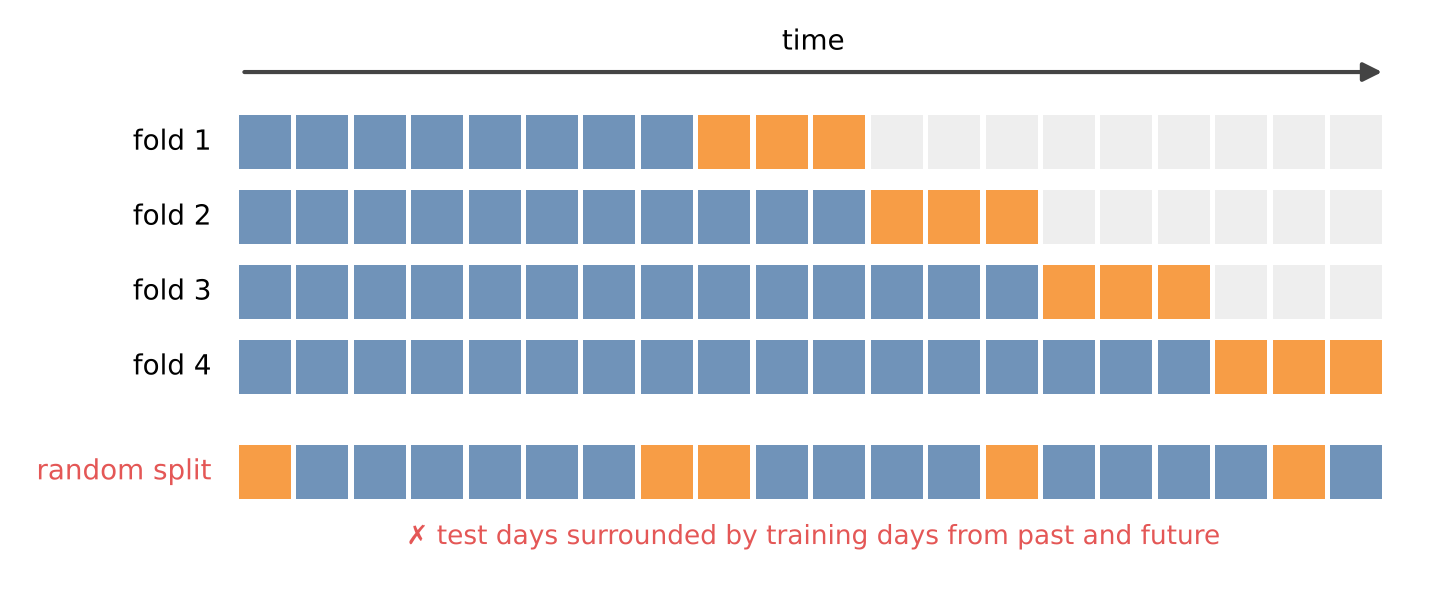
\includegraphics[width=0.9\linewidth,height=\textheight,keepaspectratio]{notebooks/images/ts-split.png}

}

\caption{\label{fig-tssplit}Time series cross-validation with an
expanding window. The model is always trained on the past (blue) and
tested on the period that immediately follows (orange). In a random
split (bottom), test observations are surrounded by training
observations from before and after.}

\end{figure}%

\begin{Shaded}
\begin{Highlighting}[]
\CommentTok{\# Setup: works locally and in Google Colab}
\ImportTok{import}\NormalTok{ importlib.util, subprocess, sys}
\ControlFlowTok{for}\NormalTok{ pkg }\KeywordTok{in}\NormalTok{ [}\StringTok{"statsmodels"}\NormalTok{, }\StringTok{"holidays"}\NormalTok{]:}
    \ControlFlowTok{if}\NormalTok{ importlib.util.find\_spec(pkg) }\KeywordTok{is} \VariableTok{None}\NormalTok{:}
\NormalTok{        subprocess.run([sys.executable, }\StringTok{"{-}m"}\NormalTok{, }\StringTok{"pip"}\NormalTok{, }\StringTok{"install"}\NormalTok{, }\StringTok{"{-}q"}\NormalTok{, pkg], check}\OperatorTok{=}\VariableTok{True}\NormalTok{)}

\ImportTok{import}\NormalTok{ numpy }\ImportTok{as}\NormalTok{ np}
\ImportTok{import}\NormalTok{ pandas }\ImportTok{as}\NormalTok{ pd}
\ImportTok{import}\NormalTok{ matplotlib.pyplot }\ImportTok{as}\NormalTok{ plt}
\ImportTok{import}\NormalTok{ seaborn }\ImportTok{as}\NormalTok{ sns}

\NormalTok{sns.set\_theme(style}\OperatorTok{=}\StringTok{"whitegrid"}\NormalTok{)}
\end{Highlighting}
\end{Shaded}

\begin{Shaded}
\begin{Highlighting}[]
\ImportTok{from}\NormalTok{ pathlib }\ImportTok{import}\NormalTok{ Path}
\ImportTok{import}\NormalTok{ requests}

\NormalTok{DATA }\OperatorTok{=}\NormalTok{ Path(}\StringTok{"data"}\NormalTok{)}
\NormalTok{DATA.mkdir(exist\_ok}\OperatorTok{=}\VariableTok{True}\NormalTok{)}

\KeywordTok{def}\NormalTok{ download(url, fname}\OperatorTok{=}\VariableTok{None}\NormalTok{):}
    \CommentTok{"""Download a file once and cache it in ./data."""}
\NormalTok{    path }\OperatorTok{=}\NormalTok{ DATA }\OperatorTok{/}\NormalTok{ (fname }\KeywordTok{or}\NormalTok{ url.split(}\StringTok{"/"}\NormalTok{)[}\OperatorTok{{-}}\DecValTok{1}\NormalTok{])}
    \ControlFlowTok{if} \KeywordTok{not}\NormalTok{ path.exists():}
\NormalTok{        r }\OperatorTok{=}\NormalTok{ requests.get(url, timeout}\OperatorTok{=}\DecValTok{300}\NormalTok{)}
\NormalTok{        r.raise\_for\_status()}
\NormalTok{        path.write\_bytes(r.content)}
    \ControlFlowTok{return}\NormalTok{ path}
\end{Highlighting}
\end{Shaded}

\section{Live coding: German electricity
load}\label{live-coding-german-electricity-load}

The Open Power System Data (OPSD) time series package collects load,
wind and solar generation and prices for 32 European countries from the
ENTSO-E Transparency Platform and other sources. We use version
2020-10-06 (2015 to mid-2020) and only the column with the actual German
load. The full CSV file is about 124 MB; we read only the two columns we
need.

\begin{Shaded}
\begin{Highlighting}[]
\NormalTok{url }\OperatorTok{=}\NormalTok{ (}\StringTok{"https://data.open{-}power{-}system{-}data.org/time\_series/2020{-}10{-}06/"}
       \StringTok{"time\_series\_60min\_singleindex.csv"}\NormalTok{)}
\NormalTok{load }\OperatorTok{=}\NormalTok{ pd.read\_csv(download(url), usecols}\OperatorTok{=}\NormalTok{[}\StringTok{"utc\_timestamp"}\NormalTok{, }\StringTok{"DE\_load\_actual\_entsoe\_transparency"}\NormalTok{],}
\NormalTok{                   parse\_dates}\OperatorTok{=}\NormalTok{[}\StringTok{"utc\_timestamp"}\NormalTok{], index\_col}\OperatorTok{=}\StringTok{"utc\_timestamp"}\NormalTok{)}
\NormalTok{load }\OperatorTok{=}\NormalTok{ load.rename(columns}\OperatorTok{=}\NormalTok{\{}\StringTok{"DE\_load\_actual\_entsoe\_transparency"}\NormalTok{: }\StringTok{"load\_MW"}\NormalTok{\})[}\StringTok{"load\_MW"}\NormalTok{]}
\NormalTok{daily }\OperatorTok{=}\NormalTok{ load.resample(}\StringTok{"D"}\NormalTok{).mean().loc[}\StringTok{"2015{-}01{-}01"}\NormalTok{:}\StringTok{"2019{-}12{-}31"}\NormalTok{] }\OperatorTok{/} \DecValTok{1000}   \CommentTok{\# GW}
\NormalTok{ax }\OperatorTok{=}\NormalTok{ daily.plot(figsize}\OperatorTok{=}\NormalTok{(}\DecValTok{10}\NormalTok{, }\DecValTok{3}\NormalTok{), ylabel}\OperatorTok{=}\StringTok{"Mean load (GW)"}\NormalTok{)}
\NormalTok{plt.show()}
\end{Highlighting}
\end{Shaded}

\pandocbounded{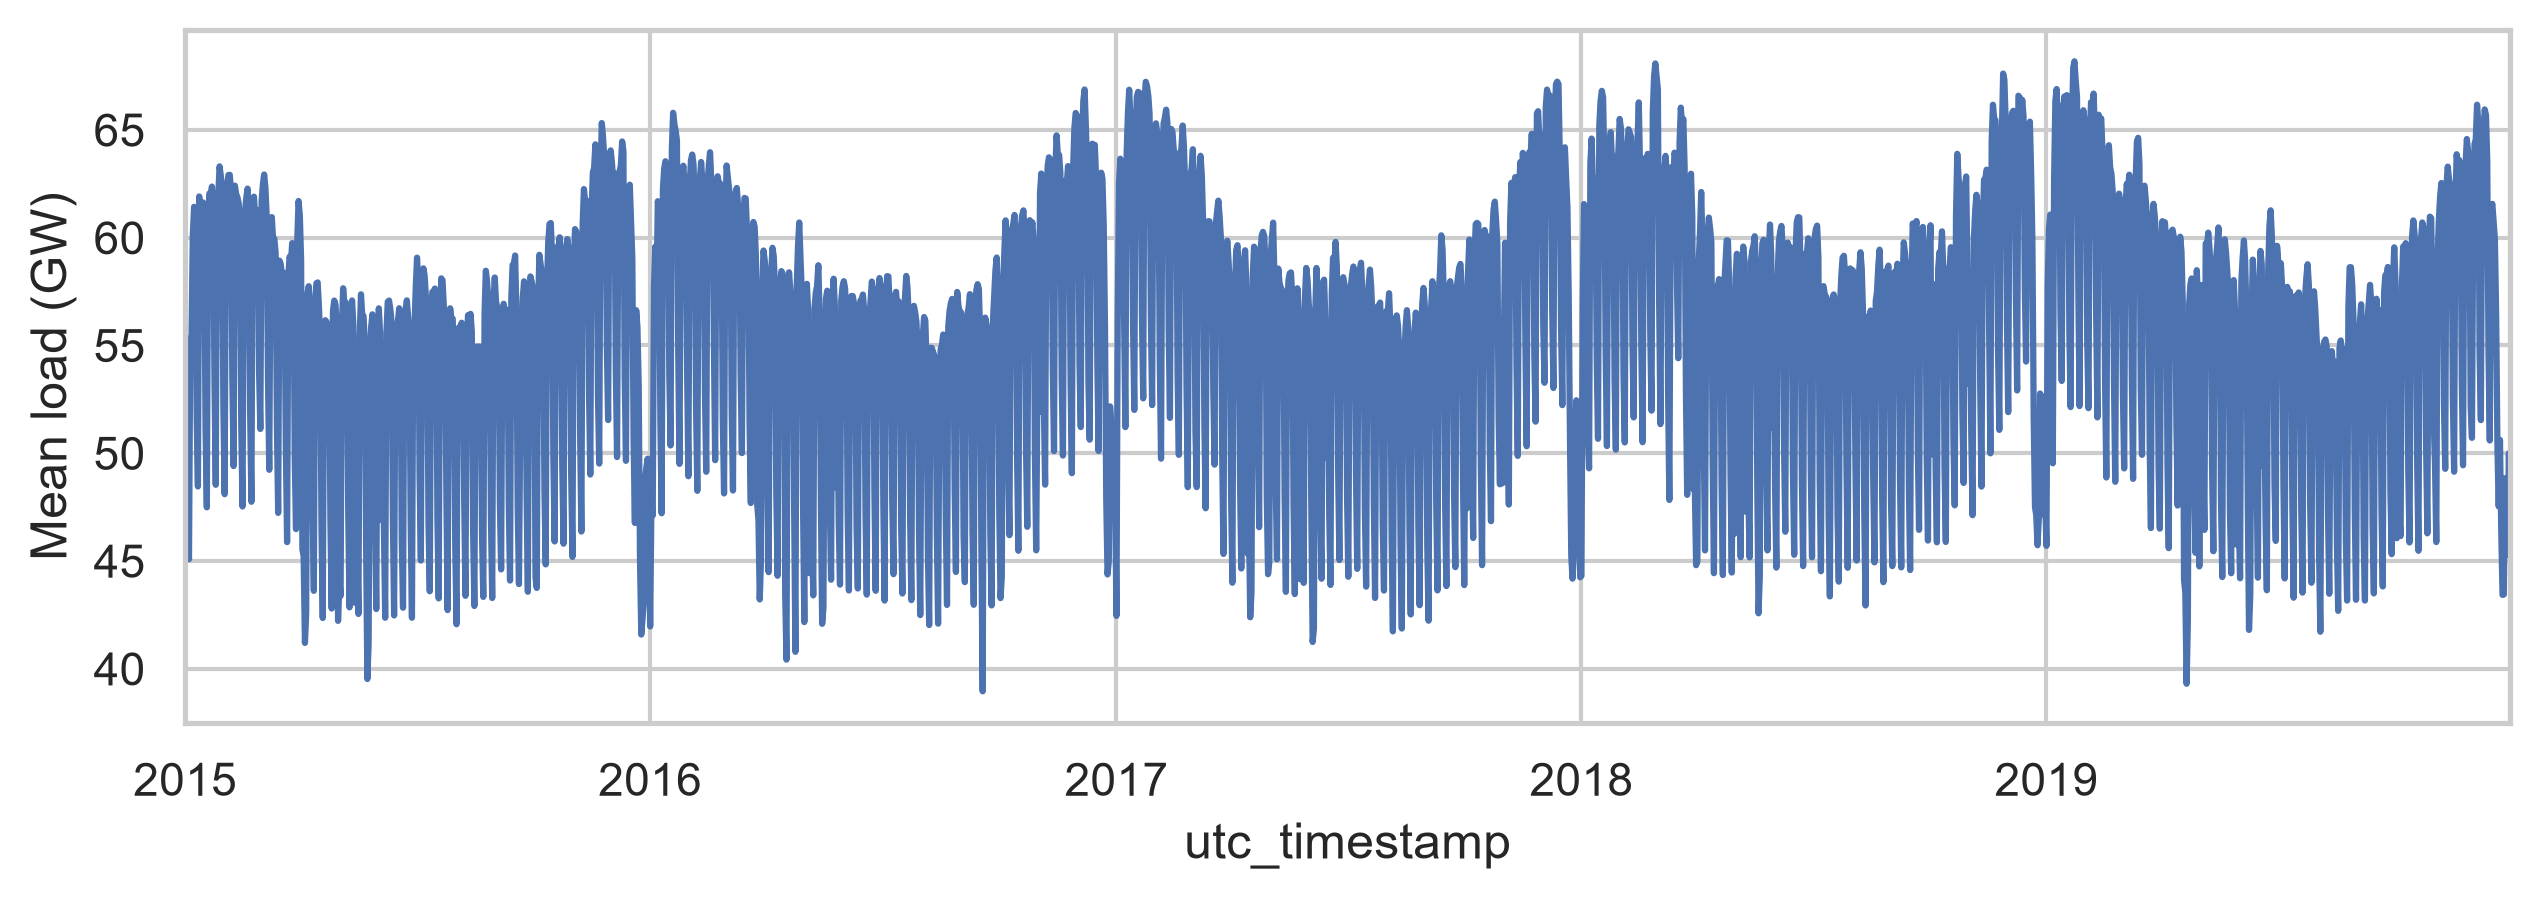
\includegraphics[keepaspectratio]{notebooks/11-time-series_files/figure-pdf/cell-4-output-1.png}}

\textbf{Discussion.} The daily mean load shows a yearly cycle (higher in
winter: lighting, heating), a strong weekly cycle (lower on weekends)
and sharp drops around Christmas and public holidays. We restrict
ourselves to 2015--2019 to avoid the exceptional Covid-19 period of 2020
-- a reminder that structural breaks can make historical data
unrepresentative.

\begin{Shaded}
\begin{Highlighting}[]
\ImportTok{from}\NormalTok{ statsmodels.graphics.tsaplots }\ImportTok{import}\NormalTok{ plot\_acf}
\NormalTok{plot\_acf(daily, lags}\OperatorTok{=}\DecValTok{40}\NormalTok{)}\OperatorTok{;}\NormalTok{ plt.show()}
\end{Highlighting}
\end{Shaded}

\pandocbounded{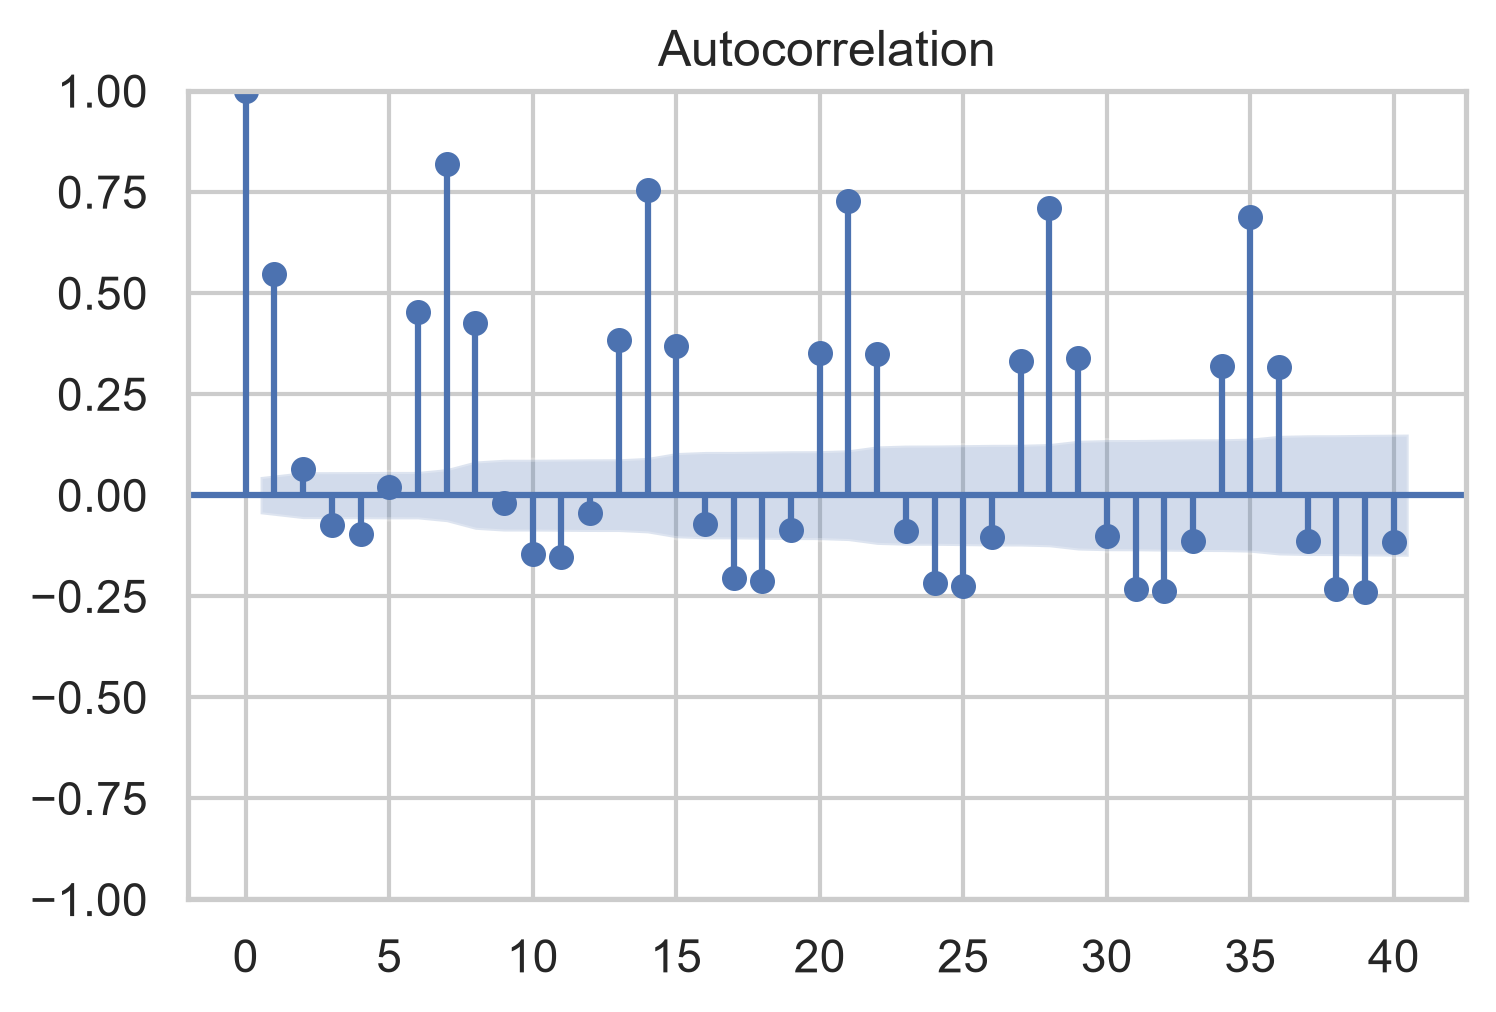
\includegraphics[keepaspectratio]{notebooks/11-time-series_files/figure-pdf/cell-5-output-1.png}}

The ACF has pronounced peaks at lags 7, 14, 21, \ldots{} -- the weekly
cycle -- and decays slowly overall, reflecting the yearly cycle and
persistence.

\subsection{Baselines}\label{baselines}

We forecast each day of the test period one day ahead (horizon 1 day)
and use the last year as test period.

\begin{Shaded}
\begin{Highlighting}[]
\NormalTok{test\_start }\OperatorTok{=} \StringTok{"2019{-}01{-}01"}
\NormalTok{y\_test }\OperatorTok{=}\NormalTok{ daily[test\_start:]}
\NormalTok{naive }\OperatorTok{=}\NormalTok{ daily.shift(}\DecValTok{1}\NormalTok{)[test\_start:]                 }\CommentTok{\# yesterday}
\NormalTok{seasonal\_naive }\OperatorTok{=}\NormalTok{ daily.shift(}\DecValTok{7}\NormalTok{)[test\_start:]        }\CommentTok{\# same weekday last week}

\KeywordTok{def}\NormalTok{ report(name, pred):}
\NormalTok{    err }\OperatorTok{=}\NormalTok{ y\_test }\OperatorTok{{-}}\NormalTok{ pred}
    \BuiltInTok{print}\NormalTok{(}\SpecialStringTok{f"}\SpecialCharTok{\{}\NormalTok{name}\SpecialCharTok{:22s\}}\SpecialStringTok{ MAE = }\SpecialCharTok{\{}\NormalTok{err}\SpecialCharTok{.}\BuiltInTok{abs}\NormalTok{()}\SpecialCharTok{.}\NormalTok{mean()}\SpecialCharTok{:.2f\}}\SpecialStringTok{ GW,  MAPE = }\SpecialCharTok{\{}\NormalTok{(err.}\BuiltInTok{abs}\NormalTok{() }\OperatorTok{/}\NormalTok{ y\_test)}\SpecialCharTok{.}\NormalTok{mean()}\SpecialCharTok{:.1\%\}}\SpecialStringTok{"}\NormalTok{)}

\NormalTok{report(}\StringTok{"naive (yesterday)"}\NormalTok{, naive)}
\NormalTok{report(}\StringTok{"seasonal naive (t{-}7)"}\NormalTok{, seasonal\_naive)}
\end{Highlighting}
\end{Shaded}

\begin{verbatim}
naive (yesterday)      MAE = 4.31 GW,  MAPE = 8.0%
seasonal naive (t-7)   MAE = 2.30 GW,  MAPE = 4.3%
\end{verbatim}

The naive forecast fails at every weekday/weekend transition; the
seasonal naive forecast handles these well and fails mainly on holidays
and around them.

\subsection{Feature-based forecasting with gradient
boosting}\label{feature-based-forecasting-with-gradient-boosting}

\begin{Shaded}
\begin{Highlighting}[]
\ImportTok{import}\NormalTok{ holidays}
\ImportTok{from}\NormalTok{ sklearn.ensemble }\ImportTok{import}\NormalTok{ HistGradientBoostingRegressor}
\ImportTok{from}\NormalTok{ sklearn.model\_selection }\ImportTok{import}\NormalTok{ TimeSeriesSplit, cross\_val\_score}

\NormalTok{df }\OperatorTok{=}\NormalTok{ daily.to\_frame(}\StringTok{"load"}\NormalTok{)}
\ControlFlowTok{for}\NormalTok{ lag }\KeywordTok{in}\NormalTok{ (}\DecValTok{1}\NormalTok{, }\DecValTok{7}\NormalTok{, }\DecValTok{14}\NormalTok{):}
\NormalTok{    df[}\SpecialStringTok{f"lag\_}\SpecialCharTok{\{}\NormalTok{lag}\SpecialCharTok{\}}\SpecialStringTok{"}\NormalTok{] }\OperatorTok{=}\NormalTok{ df[}\StringTok{"load"}\NormalTok{].shift(lag)}
\NormalTok{df[}\StringTok{"dow"}\NormalTok{] }\OperatorTok{=}\NormalTok{ df.index.dayofweek}
\NormalTok{df[}\StringTok{"doy"}\NormalTok{] }\OperatorTok{=}\NormalTok{ df.index.dayofyear}
\NormalTok{de\_holidays }\OperatorTok{=}\NormalTok{ holidays.Germany(years}\OperatorTok{=}\BuiltInTok{range}\NormalTok{(}\DecValTok{2015}\NormalTok{, }\DecValTok{2021}\NormalTok{))}
\NormalTok{df[}\StringTok{"holiday"}\NormalTok{] }\OperatorTok{=}\NormalTok{ [d.date() }\KeywordTok{in}\NormalTok{ de\_holidays }\ControlFlowTok{for}\NormalTok{ d }\KeywordTok{in}\NormalTok{ df.index]}
\NormalTok{df }\OperatorTok{=}\NormalTok{ df.dropna()}

\NormalTok{X, y }\OperatorTok{=}\NormalTok{ df.drop(columns}\OperatorTok{=}\StringTok{"load"}\NormalTok{), df[}\StringTok{"load"}\NormalTok{]}
\NormalTok{gbr }\OperatorTok{=}\NormalTok{ HistGradientBoostingRegressor(random\_state}\OperatorTok{=}\DecValTok{0}\NormalTok{)}
\NormalTok{scores }\OperatorTok{=}\NormalTok{ cross\_val\_score(gbr, X, y, cv}\OperatorTok{=}\NormalTok{TimeSeriesSplit(}\DecValTok{5}\NormalTok{), scoring}\OperatorTok{=}\StringTok{"neg\_mean\_absolute\_percentage\_error"}\NormalTok{)}
\BuiltInTok{print}\NormalTok{(}\StringTok{"MAPE per fold (time series CV):"}\NormalTok{, np.}\BuiltInTok{round}\NormalTok{(}\OperatorTok{{-}}\NormalTok{scores, }\DecValTok{3}\NormalTok{))}

\NormalTok{gbr.fit(X[:test\_start].iloc[:}\OperatorTok{{-}}\DecValTok{1}\NormalTok{], y[:test\_start].iloc[:}\OperatorTok{{-}}\DecValTok{1}\NormalTok{])}
\NormalTok{report(}\StringTok{"gradient boosting"}\NormalTok{, pd.Series(gbr.predict(X[test\_start:]), index}\OperatorTok{=}\NormalTok{X[test\_start:].index))}
\end{Highlighting}
\end{Shaded}

\begin{verbatim}
MAPE per fold (time series CV): [0.032 0.029 0.018 0.016 0.016]
gradient boosting      MAE = 0.88 GW,  MAPE = 1.6%
\end{verbatim}

\textbf{Discussion.} All features are available at forecast time: lags
1, 7 and 14 days, the calendar and the holiday calendar, which is known
in advance. \texttt{TimeSeriesSplit} trains on an expanding window and
always tests on the following block; the error per fold shows how stable
the model is over time. The comparison with the baselines on the same
test year shows how much the model really adds.

\textbf{Weather as an input.} Temperature drives heating and cooling
demand. Historical hourly temperatures are available from the DWD (see
Chapter 2 and Exercise 2). For a real day-ahead forecast, the model must
be trained and operated with temperature \emph{forecasts} -- using
measured temperatures overstates the accuracy.

\section{Back to the decision}\label{back-to-the-decision-10}

We compare both methods on the test year 2019, which was not used for
training. The model must reduce the MAE by at least 10 \%.

\begin{Shaded}
\begin{Highlighting}[]
\NormalTok{pred\_gb }\OperatorTok{=}\NormalTok{ pd.Series(gbr.predict(X[test\_start:]), index}\OperatorTok{=}\NormalTok{X[test\_start:].index)}
\NormalTok{common }\OperatorTok{=}\NormalTok{ pred\_gb.index.intersection(seasonal\_naive.dropna().index)}
\NormalTok{mae\_naive }\OperatorTok{=}\NormalTok{ (y\_test[common] }\OperatorTok{{-}}\NormalTok{ seasonal\_naive[common]).}\BuiltInTok{abs}\NormalTok{().mean()}
\NormalTok{mae\_model }\OperatorTok{=}\NormalTok{ (y\_test[common] }\OperatorTok{{-}}\NormalTok{ pred\_gb[common]).}\BuiltInTok{abs}\NormalTok{().mean()}
\NormalTok{gain }\OperatorTok{=} \DecValTok{1} \OperatorTok{{-}}\NormalTok{ mae\_model }\OperatorTok{/}\NormalTok{ mae\_naive}
\BuiltInTok{print}\NormalTok{(}\SpecialStringTok{f"MAE seasonal naive: }\SpecialCharTok{\{}\NormalTok{mae\_naive}\SpecialCharTok{:.2f\}}\SpecialStringTok{ GW,  MAE gradient boosting: }\SpecialCharTok{\{}\NormalTok{mae\_model}\SpecialCharTok{:.2f\}}\SpecialStringTok{ GW,  improvement: }\SpecialCharTok{\{}\NormalTok{gain}\SpecialCharTok{:.0\%\}}\SpecialStringTok{"}\NormalTok{)}
\BuiltInTok{print}\NormalTok{(}\StringTok{"Decision:"}\NormalTok{, }\StringTok{"replace the seasonal naive forecast."} \ControlFlowTok{if}\NormalTok{ gain }\OperatorTok{\textgreater{}=} \FloatTok{0.10} \ControlFlowTok{else} \StringTok{"keep the seasonal naive forecast."}\NormalTok{)}
\end{Highlighting}
\end{Shaded}

\begin{verbatim}
MAE seasonal naive: 2.30 GW,  MAE gradient boosting: 0.88 GW,  improvement: 62%
Decision: replace the seasonal naive forecast.
\end{verbatim}

A one-year test is a good basis, but the recommendation should add: the
improvement comes mainly from holidays and transitions -- check the
error on those days separately; the model should be monitored after
go-live, because structural changes (such as the drop in demand in 2020)
can make it worse than the simple method; and adding temperature
forecasts (Exercise 2) is the obvious next step.

\section{Extension: seasonal ARIMA}\label{extension-seasonal-arima}

\emph{Extension -- optional material, not required for the exam.}

ARIMA models describe a series by its own past values (\textbf{AR},
autoregressive part), past forecast errors (\textbf{MA}, moving average
part) after differencing \(d\) times (\textbf{I}, integrated). The
seasonal extension SARIMA\((p,d,q)(P,D,Q)_s\) adds the same terms at the
seasonal lag \(s\) (here \(s = 7\) days). ARIMA models are the classical
statistical approach: compact, with well-founded prediction intervals,
but harder to extend with many exogenous variables than the regression
approach.

\begin{Shaded}
\begin{Highlighting}[]
\ImportTok{from}\NormalTok{ statsmodels.tsa.statespace.sarimax }\ImportTok{import}\NormalTok{ SARIMAX}

\NormalTok{train, test }\OperatorTok{=}\NormalTok{ daily[:}\StringTok{"2019{-}10{-}31"}\NormalTok{], daily[}\StringTok{"2019{-}11{-}01"}\NormalTok{:}\StringTok{"2019{-}11{-}30"}\NormalTok{]}
\NormalTok{sarima }\OperatorTok{=}\NormalTok{ SARIMAX(train, order}\OperatorTok{=}\NormalTok{(}\DecValTok{1}\NormalTok{, }\DecValTok{0}\NormalTok{, }\DecValTok{1}\NormalTok{), seasonal\_order}\OperatorTok{=}\NormalTok{(}\DecValTok{1}\NormalTok{, }\DecValTok{1}\NormalTok{, }\DecValTok{1}\NormalTok{, }\DecValTok{7}\NormalTok{)).fit(disp}\OperatorTok{=}\VariableTok{False}\NormalTok{)}
\NormalTok{fc }\OperatorTok{=}\NormalTok{ sarima.get\_forecast(}\BuiltInTok{len}\NormalTok{(test))}
\NormalTok{ax }\OperatorTok{=}\NormalTok{ train[}\StringTok{"2019{-}09{-}01"}\NormalTok{:].plot(label}\OperatorTok{=}\StringTok{"train"}\NormalTok{, figsize}\OperatorTok{=}\NormalTok{(}\DecValTok{10}\NormalTok{, }\DecValTok{3}\NormalTok{))}
\NormalTok{test.plot(ax}\OperatorTok{=}\NormalTok{ax, label}\OperatorTok{=}\StringTok{"actual"}\NormalTok{)}
\NormalTok{fc.predicted\_mean.plot(ax}\OperatorTok{=}\NormalTok{ax, label}\OperatorTok{=}\StringTok{"SARIMA forecast"}\NormalTok{)}
\NormalTok{ci }\OperatorTok{=}\NormalTok{ fc.conf\_int()}
\NormalTok{ax.fill\_between(ci.index, ci.iloc[:, }\DecValTok{0}\NormalTok{], ci.iloc[:, }\DecValTok{1}\NormalTok{], alpha}\OperatorTok{=}\FloatTok{0.2}\NormalTok{)}
\NormalTok{ax.legend()}\OperatorTok{;}\NormalTok{ plt.show()}
\NormalTok{mape }\OperatorTok{=}\NormalTok{ (}\BuiltInTok{abs}\NormalTok{(fc.predicted\_mean }\OperatorTok{{-}}\NormalTok{ test) }\OperatorTok{/}\NormalTok{ test).mean()}
\BuiltInTok{print}\NormalTok{(}\SpecialStringTok{f"MAPE November 2019 (forecast up to 30 days ahead): }\SpecialCharTok{\{}\NormalTok{mape}\SpecialCharTok{:.1\%\}}\SpecialStringTok{"}\NormalTok{)}
\end{Highlighting}
\end{Shaded}

\pandocbounded{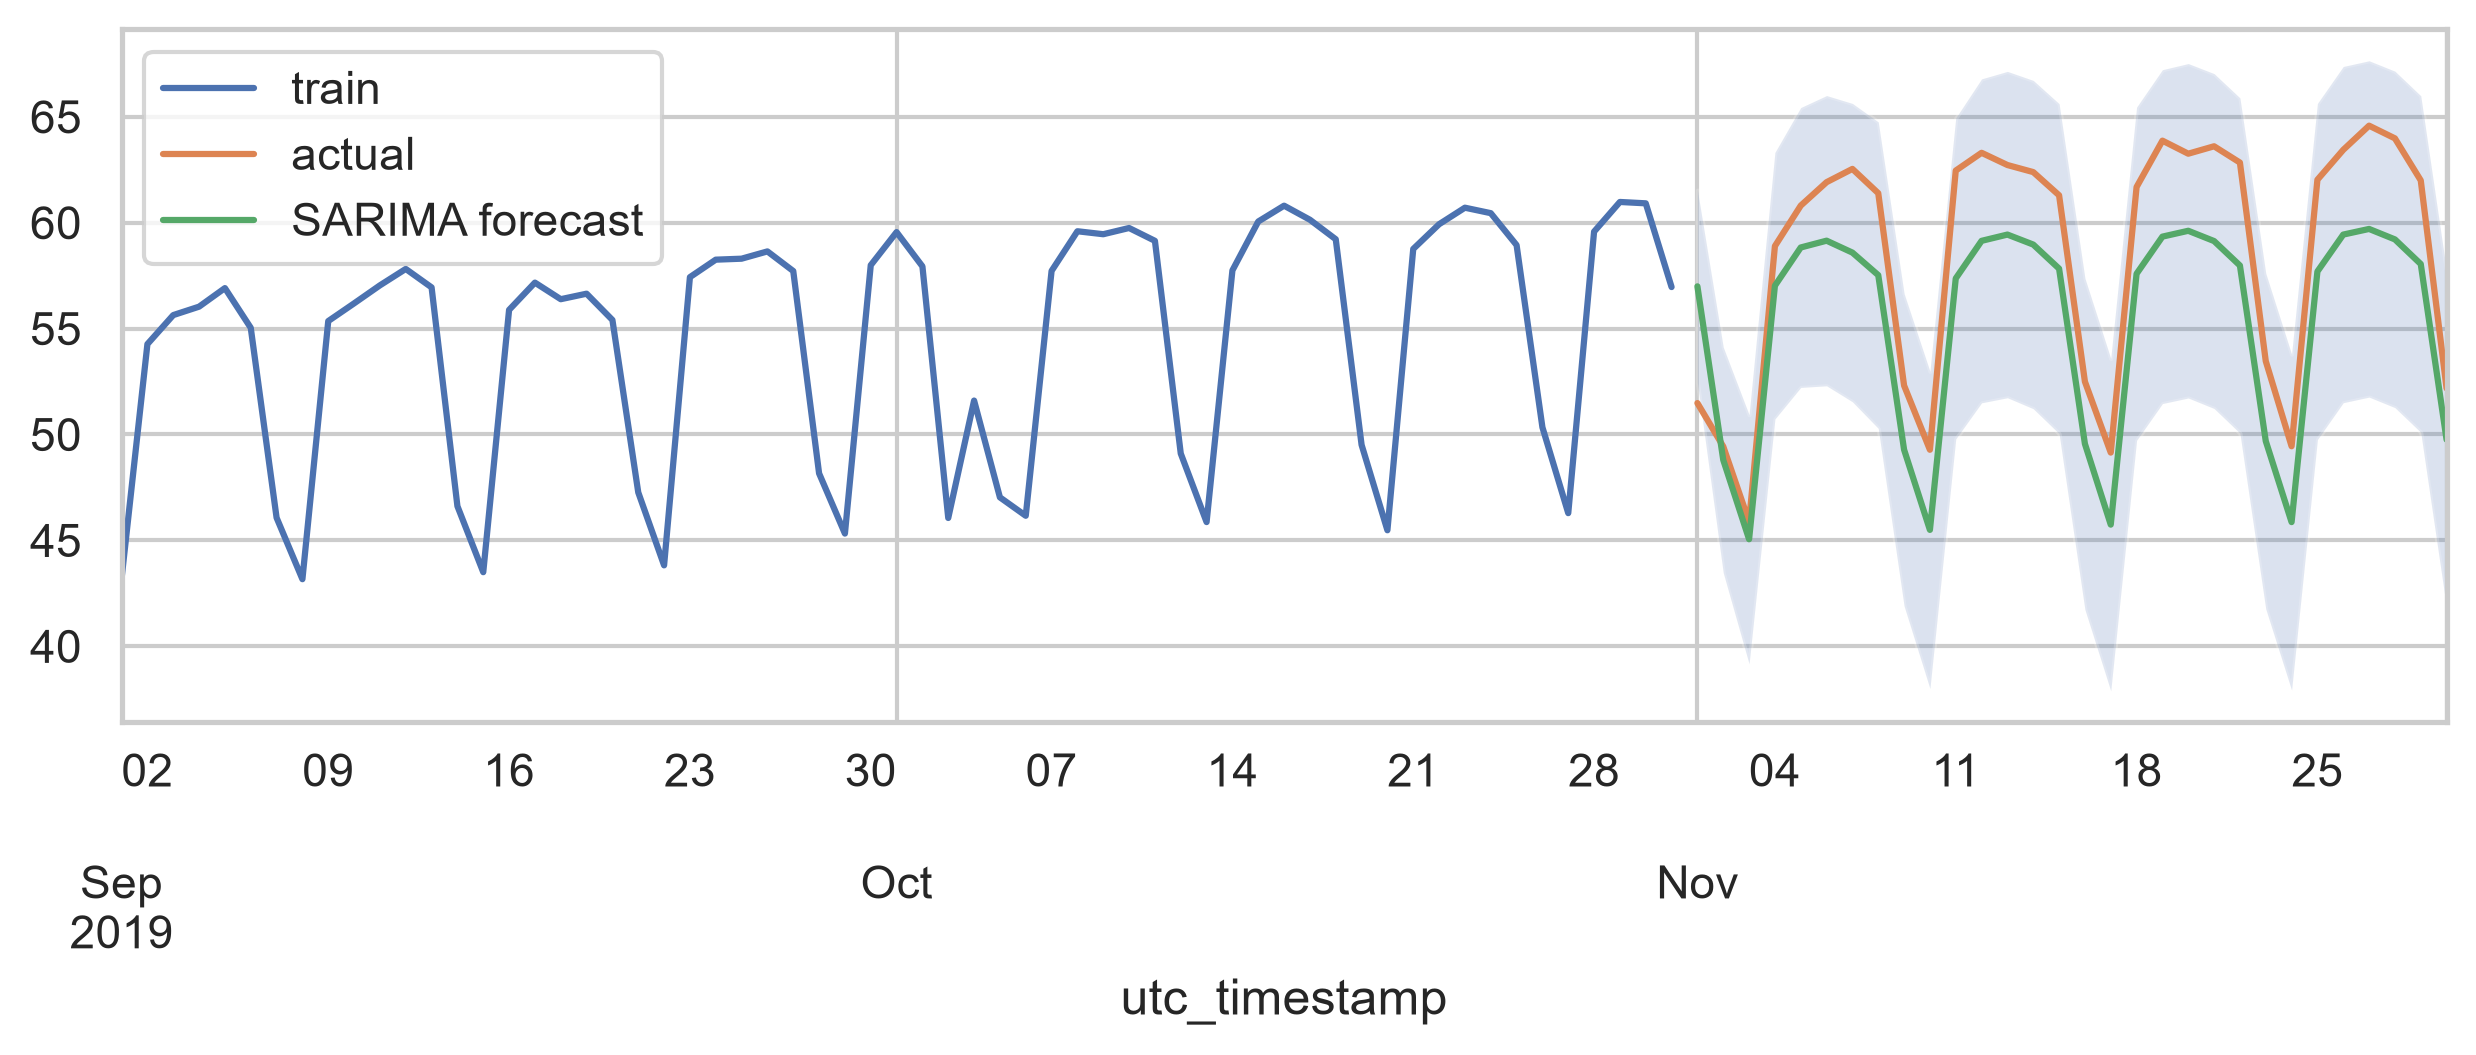
\includegraphics[keepaspectratio]{notebooks/11-time-series_files/figure-pdf/cell-9-output-1.png}}

\begin{verbatim}
MAPE November 2019 (forecast up to 30 days ahead): 6.1%
\end{verbatim}

Note that this is a \emph{multi-step} forecast: all 30 days are forecast
at once from the end of October, so the horizon grows from 1 to 30 days,
and the prediction interval widens accordingly. It is therefore not
directly comparable with the one-day-ahead forecasts above.

\begin{tcolorbox}[enhanced jigsaw, colframe=quarto-callout-important-color-frame, toprule=.15mm, rightrule=.15mm, title=\textcolor{quarto-callout-important-color}{\faExclamation}\hspace{0.5em}{Key takeaways}, colbacktitle=quarto-callout-important-color!10!white, left=2mm, titlerule=0mm, bottomtitle=1mm, toptitle=1mm, opacityback=0, bottomrule=.15mm, breakable, arc=.35mm, opacitybacktitle=0.6, colback=white, coltitle=black, leftrule=.75mm]

\begin{itemize}
\tightlist
\item
  Define horizon and information set first; they determine which
  features are legal.
\item
  Always compare with naive and seasonal naive baselines.
\item
  Lag, calendar and exogenous features turn forecasting into regression;
  gradient boosting is a strong default.
\item
  Validate in time order (\texttt{TimeSeriesSplit}); random splits and
  future information produce misleadingly small errors.
\end{itemize}

\end{tcolorbox}

\section{Exercises}\label{exercises-10}

\begin{enumerate}
\def\labelenumi{\arabic{enumi}.}
\tightlist
\item
  Use a random 5-fold \texttt{KFold} with shuffling instead of
  \texttt{TimeSeriesSplit} for the gradient boosting model. Why does the
  error look better -- and why is that wrong?
\item
  Add the daily mean temperature of the DWD station Trier-Petrisberg
  (historical hourly data) as a feature. How much does the error
  improve? Why is this improvement optimistic for real operation?
\item
  Remove the \texttt{holiday} feature. On which days does the error
  increase most?
\item
  Build a forecast for 7 days ahead (e.g.~for weekly planning). Which
  lag features may you still use? How does the error compare with the
  1-day-ahead forecast?
\item
  You want to forecast \emph{hourly} load one day ahead. Which seasonal
  periods and which lags are relevant now?
\end{enumerate}

\subsection{Solutions}\label{solutions-10}

\begin{tcolorbox}[enhanced jigsaw, colframe=quarto-callout-caution-color-frame, toprule=.15mm, rightrule=.15mm, title=\textcolor{quarto-callout-caution-color}{\faFire}\hspace{0.5em}{Solution to Exercise 1}, colbacktitle=quarto-callout-caution-color!10!white, left=2mm, titlerule=0mm, bottomtitle=1mm, toptitle=1mm, opacityback=0, bottomrule=.15mm, breakable, arc=.35mm, opacitybacktitle=0.6, colback=white, coltitle=black, leftrule=.75mm]

\begin{Shaded}
\begin{Highlighting}[]
\ImportTok{from}\NormalTok{ sklearn.model\_selection }\ImportTok{import}\NormalTok{ KFold}

\NormalTok{random\_scores }\OperatorTok{=}\NormalTok{ cross\_val\_score(gbr, X, y, cv}\OperatorTok{=}\NormalTok{KFold(}\DecValTok{5}\NormalTok{, shuffle}\OperatorTok{=}\VariableTok{True}\NormalTok{, random\_state}\OperatorTok{=}\DecValTok{0}\NormalTok{),}
\NormalTok{                                scoring}\OperatorTok{=}\StringTok{"neg\_mean\_absolute\_percentage\_error"}\NormalTok{)}
\BuiltInTok{print}\NormalTok{(}\StringTok{"MAPE random KFold:      "}\NormalTok{, np.}\BuiltInTok{round}\NormalTok{(}\OperatorTok{{-}}\NormalTok{random\_scores, }\DecValTok{3}\NormalTok{))}
\BuiltInTok{print}\NormalTok{(}\StringTok{"MAPE TimeSeriesSplit:   "}\NormalTok{, np.}\BuiltInTok{round}\NormalTok{(}\OperatorTok{{-}}\NormalTok{scores, }\DecValTok{3}\NormalTok{))}
\end{Highlighting}
\end{Shaded}

\begin{verbatim}
MAPE random KFold:       [0.016 0.016 0.015 0.014 0.016]
MAPE TimeSeriesSplit:    [0.032 0.029 0.018 0.016 0.016]
\end{verbatim}

With random folds, every test day is surrounded by training days from
just before and just after. The model effectively interpolates within
known periods -- it has, for instance, seen the Christmas holidays of
the same year. In operation, the future is never available for training.
The time-ordered split measures what we need: the error on a period that
lies entirely after the training data.

\end{tcolorbox}

\begin{tcolorbox}[enhanced jigsaw, colframe=quarto-callout-caution-color-frame, toprule=.15mm, rightrule=.15mm, title=\textcolor{quarto-callout-caution-color}{\faFire}\hspace{0.5em}{Solution to Exercise 2}, colbacktitle=quarto-callout-caution-color!10!white, left=2mm, titlerule=0mm, bottomtitle=1mm, toptitle=1mm, opacityback=0, bottomrule=.15mm, breakable, arc=.35mm, opacitybacktitle=0.6, colback=white, coltitle=black, leftrule=.75mm]

\begin{Shaded}
\begin{Highlighting}[]
\ImportTok{import}\NormalTok{ re, zipfile}

\NormalTok{hist\_dir }\OperatorTok{=}\NormalTok{ (}\StringTok{"https://opendata.dwd.de/climate\_environment/CDC/observations\_germany/"}
            \StringTok{"climate/hourly/air\_temperature/historical/"}\NormalTok{)}
\NormalTok{listing }\OperatorTok{=}\NormalTok{ download(hist\_dir, }\StringTok{"dwd\_hist\_index.html"}\NormalTok{).read\_text()}
\NormalTok{fname }\OperatorTok{=}\NormalTok{ re.search(}\VerbatimStringTok{r"stundenwerte\_TU\_05100\_\textbackslash{}d+\_\textbackslash{}d+\_hist\textbackslash{}.zip"}\NormalTok{, listing).group(}\DecValTok{0}\NormalTok{)}
\ControlFlowTok{with}\NormalTok{ zipfile.ZipFile(download(hist\_dir }\OperatorTok{+}\NormalTok{ fname)) }\ImportTok{as}\NormalTok{ z:}
\NormalTok{    name }\OperatorTok{=} \BuiltInTok{next}\NormalTok{(n }\ControlFlowTok{for}\NormalTok{ n }\KeywordTok{in}\NormalTok{ z.namelist() }\ControlFlowTok{if}\NormalTok{ n.startswith(}\StringTok{"produkt"}\NormalTok{))}
\NormalTok{    dwd }\OperatorTok{=}\NormalTok{ pd.read\_csv(z.}\BuiltInTok{open}\NormalTok{(name), sep}\OperatorTok{=}\StringTok{";"}\NormalTok{, na\_values}\OperatorTok{=}\NormalTok{[}\OperatorTok{{-}}\DecValTok{999}\NormalTok{], skipinitialspace}\OperatorTok{=}\VariableTok{True}\NormalTok{)}
\NormalTok{dwd.columns }\OperatorTok{=}\NormalTok{ dwd.columns.}\BuiltInTok{str}\NormalTok{.strip()}
\NormalTok{dwd[}\StringTok{"time"}\NormalTok{] }\OperatorTok{=}\NormalTok{ pd.to\_datetime(dwd[}\StringTok{"MESS\_DATUM"}\NormalTok{].astype(}\BuiltInTok{str}\NormalTok{), }\BuiltInTok{format}\OperatorTok{=}\StringTok{"\%Y\%m}\SpecialCharTok{\%d}\StringTok{\%H"}\NormalTok{)}
\NormalTok{temp }\OperatorTok{=}\NormalTok{ dwd.set\_index(}\StringTok{"time"}\NormalTok{)[}\StringTok{"TT\_TU"}\NormalTok{].resample(}\StringTok{"D"}\NormalTok{).mean().rename(}\StringTok{"temp"}\NormalTok{)}
\NormalTok{temp.index }\OperatorTok{=}\NormalTok{ temp.index.tz\_localize(}\StringTok{"UTC"}\NormalTok{)          }\CommentTok{\# DWD time stamps are UTC, like the OPSD index}

\NormalTok{df\_t }\OperatorTok{=}\NormalTok{ df.join(temp, how}\OperatorTok{=}\StringTok{"inner"}\NormalTok{).dropna()}
\NormalTok{X\_t, y\_t }\OperatorTok{=}\NormalTok{ df\_t.drop(columns}\OperatorTok{=}\StringTok{"load"}\NormalTok{), df\_t[}\StringTok{"load"}\NormalTok{]}
\NormalTok{s\_t }\OperatorTok{=}\NormalTok{ cross\_val\_score(gbr, X\_t, y\_t, cv}\OperatorTok{=}\NormalTok{TimeSeriesSplit(}\DecValTok{5}\NormalTok{), scoring}\OperatorTok{=}\StringTok{"neg\_mean\_absolute\_percentage\_error"}\NormalTok{)}
\BuiltInTok{print}\NormalTok{(}\SpecialStringTok{f"MAPE without temperature: }\SpecialCharTok{\{}\OperatorTok{{-}}\NormalTok{scores}\SpecialCharTok{.}\NormalTok{mean()}\SpecialCharTok{:.3f\}}\SpecialStringTok{,  with temperature: }\SpecialCharTok{\{}\OperatorTok{{-}}\NormalTok{s\_t}\SpecialCharTok{.}\NormalTok{mean()}\SpecialCharTok{:.3f\}}\SpecialStringTok{"}\NormalTok{)}
\end{Highlighting}
\end{Shaded}

\begin{verbatim}
MAPE without temperature: 0.022,  with temperature: 0.022
\end{verbatim}

The temperature helps mostly in the heating season. The improvement is
optimistic for two reasons: we use the \emph{measured} temperature of
the forecast day, which is not known one day in advance (in operation
one would use a weather forecast with its own error), and one station is
only a rough proxy for the temperature relevant to German demand -- a
population-weighted average of many stations would be better.

\end{tcolorbox}

\begin{tcolorbox}[enhanced jigsaw, colframe=quarto-callout-caution-color-frame, toprule=.15mm, rightrule=.15mm, title=\textcolor{quarto-callout-caution-color}{\faFire}\hspace{0.5em}{Solution to Exercise 3}, colbacktitle=quarto-callout-caution-color!10!white, left=2mm, titlerule=0mm, bottomtitle=1mm, toptitle=1mm, opacityback=0, bottomrule=.15mm, breakable, arc=.35mm, opacitybacktitle=0.6, colback=white, coltitle=black, leftrule=.75mm]

\begin{Shaded}
\begin{Highlighting}[]
\NormalTok{X\_nh }\OperatorTok{=}\NormalTok{ X.drop(columns}\OperatorTok{=}\StringTok{"holiday"}\NormalTok{)}
\NormalTok{m\_h }\OperatorTok{=}\NormalTok{ HistGradientBoostingRegressor(random\_state}\OperatorTok{=}\DecValTok{0}\NormalTok{).fit(X[:test\_start].iloc[:}\OperatorTok{{-}}\DecValTok{1}\NormalTok{], y[:test\_start].iloc[:}\OperatorTok{{-}}\DecValTok{1}\NormalTok{])}
\NormalTok{m\_nh }\OperatorTok{=}\NormalTok{ HistGradientBoostingRegressor(random\_state}\OperatorTok{=}\DecValTok{0}\NormalTok{).fit(X\_nh[:test\_start].iloc[:}\OperatorTok{{-}}\DecValTok{1}\NormalTok{], y[:test\_start].iloc[:}\OperatorTok{{-}}\DecValTok{1}\NormalTok{])}
\NormalTok{err\_h }\OperatorTok{=}\NormalTok{ (y[test\_start:] }\OperatorTok{{-}}\NormalTok{ m\_h.predict(X[test\_start:])).}\BuiltInTok{abs}\NormalTok{()}
\NormalTok{err\_nh }\OperatorTok{=}\NormalTok{ (y[test\_start:] }\OperatorTok{{-}}\NormalTok{ m\_nh.predict(X\_nh[test\_start:])).}\BuiltInTok{abs}\NormalTok{()}
\NormalTok{(err\_nh }\OperatorTok{{-}}\NormalTok{ err\_h).sort\_values(ascending}\OperatorTok{=}\VariableTok{False}\NormalTok{).head(}\DecValTok{10}\NormalTok{).}\BuiltInTok{round}\NormalTok{(}\DecValTok{2}\NormalTok{)}
\end{Highlighting}
\end{Shaded}

\begin{verbatim}
utc_timestamp
2019-05-01 00:00:00+00:00    12.21
2019-01-01 00:00:00+00:00    11.70
2019-10-03 00:00:00+00:00    10.18
2019-04-19 00:00:00+00:00     9.58
2019-06-10 00:00:00+00:00     9.51
2019-04-23 00:00:00+00:00     5.61
2019-04-22 00:00:00+00:00     4.81
2019-12-25 00:00:00+00:00     4.00
2019-05-02 00:00:00+00:00     3.24
2019-05-27 00:00:00+00:00     2.95
Name: load, dtype: float64
\end{verbatim}

The largest increases occur on public holidays (Easter, Whit Monday,
Christmas, New Year) and often on the following days, because the lag-1
and lag-7 features then contain the unusual holiday load. A ``bridge
day'' feature or a feature ``holiday 7 days ago'' can reduce these
after-effects.

\end{tcolorbox}

\begin{tcolorbox}[enhanced jigsaw, colframe=quarto-callout-caution-color-frame, toprule=.15mm, rightrule=.15mm, title=\textcolor{quarto-callout-caution-color}{\faFire}\hspace{0.5em}{Solution to Exercise 4}, colbacktitle=quarto-callout-caution-color!10!white, left=2mm, titlerule=0mm, bottomtitle=1mm, toptitle=1mm, opacityback=0, bottomrule=.15mm, breakable, arc=.35mm, opacitybacktitle=0.6, colback=white, coltitle=black, leftrule=.75mm]

\begin{Shaded}
\begin{Highlighting}[]
\NormalTok{h }\OperatorTok{=} \DecValTok{7}
\NormalTok{df7 }\OperatorTok{=}\NormalTok{ daily.to\_frame(}\StringTok{"load"}\NormalTok{)}
\ControlFlowTok{for}\NormalTok{ lag }\KeywordTok{in}\NormalTok{ (h, h }\OperatorTok{+} \DecValTok{7}\NormalTok{, }\DecValTok{364}\NormalTok{):}
\NormalTok{    df7[}\SpecialStringTok{f"lag\_}\SpecialCharTok{\{}\NormalTok{lag}\SpecialCharTok{\}}\SpecialStringTok{"}\NormalTok{] }\OperatorTok{=}\NormalTok{ df7[}\StringTok{"load"}\NormalTok{].shift(lag)}
\NormalTok{df7[}\StringTok{"dow"}\NormalTok{], df7[}\StringTok{"doy"}\NormalTok{] }\OperatorTok{=}\NormalTok{ df7.index.dayofweek, df7.index.dayofyear}
\NormalTok{df7[}\StringTok{"holiday"}\NormalTok{] }\OperatorTok{=}\NormalTok{ [d.date() }\KeywordTok{in}\NormalTok{ de\_holidays }\ControlFlowTok{for}\NormalTok{ d }\KeywordTok{in}\NormalTok{ df7.index]}
\NormalTok{df7 }\OperatorTok{=}\NormalTok{ df7.dropna()}
\NormalTok{s7 }\OperatorTok{=}\NormalTok{ cross\_val\_score(HistGradientBoostingRegressor(random\_state}\OperatorTok{=}\DecValTok{0}\NormalTok{), df7.drop(columns}\OperatorTok{=}\StringTok{"load"}\NormalTok{), df7[}\StringTok{"load"}\NormalTok{],}
\NormalTok{                     cv}\OperatorTok{=}\NormalTok{TimeSeriesSplit(}\DecValTok{5}\NormalTok{), scoring}\OperatorTok{=}\StringTok{"neg\_mean\_absolute\_percentage\_error"}\NormalTok{)}
\BuiltInTok{print}\NormalTok{(}\SpecialStringTok{f"MAPE 1 day ahead: }\SpecialCharTok{\{}\OperatorTok{{-}}\NormalTok{scores}\SpecialCharTok{.}\NormalTok{mean()}\SpecialCharTok{:.3f\}}\SpecialStringTok{,  7 days ahead: }\SpecialCharTok{\{}\OperatorTok{{-}}\NormalTok{s7}\SpecialCharTok{.}\NormalTok{mean()}\SpecialCharTok{:.3f\}}\SpecialStringTok{"}\NormalTok{)}
\end{Highlighting}
\end{Shaded}

\begin{verbatim}
MAPE 1 day ahead: 0.022,  7 days ahead: 0.033
\end{verbatim}

For a 7-day horizon, the most recent load we can use is from 7 days
before the target day, so lags 1 to 6 are forbidden. Lags 7, 14 and the
same day one year ago (lag 364, which keeps the weekday) remain. The
error typically increases because recent changes -- a cold spell, a
holiday period -- are not yet visible in the data.

\end{tcolorbox}

\begin{tcolorbox}[enhanced jigsaw, colframe=quarto-callout-caution-color-frame, toprule=.15mm, rightrule=.15mm, title=\textcolor{quarto-callout-caution-color}{\faFire}\hspace{0.5em}{Solution to Exercise 5}, colbacktitle=quarto-callout-caution-color!10!white, left=2mm, titlerule=0mm, bottomtitle=1mm, toptitle=1mm, opacityback=0, bottomrule=.15mm, breakable, arc=.35mm, opacitybacktitle=0.6, colback=white, coltitle=black, leftrule=.75mm]

Hourly load has a \textbf{daily} cycle (period 24 h), a \textbf{weekly}
cycle (168 h) and a yearly cycle (8760 h), and the daily profile itself
differs between weekdays and weekends and between summer and winter
(interaction of calendar features). For a day-ahead forecast made, say,
at noon for all 24 hours of the next day, the most recent usable lags
are around 24--36 hours, plus 168 hours (same hour last week). Useful
features: hour of day, weekday, holiday, lags of 24, 48 and 168 hours,
and temperature forecasts. Also note daylight saving time: in local
time, one day per year has 23 and one 25 hours -- working in UTC and
adding local-time calendar features avoids errors.

\end{tcolorbox}

\chapter{Deep Learning in
Engineering}\label{deep-learning-in-engineering}

Neural networks are behind most of the recent headlines about artificial
intelligence: image recognition, speech assistants, large language
models. In engineering, they are used for visual quality inspection, for
virtual sensors, for surrogate models of simulations and for predicting
the remaining useful life of machines. Their strength is that they can
learn suitable features from raw data -- pixels, signal samples,
sequences -- by themselves, where the methods of the previous chapters
needed hand-crafted features.

This chapter gives a compact, application-oriented introduction. We
build a neural network from its smallest unit, the neuron, train it with
gradient descent and apply it to predict the remaining useful life of
jet engines. An extension section shows how pretrained networks detect
defects on images. Neural networks in depth are the subject of a
separate course; here the goal is to understand the principles and to
judge when deep learning is worth its cost.

\textbf{Scenario: from fixed intervals to condition-based maintenance}

In Chapter 3, the airline set a fixed overhaul interval for its engines.
The fleet manager now wants to go further: every engine streams its
sensor data, and a model predicts its remaining useful life (RUL). An
engine should be scheduled for overhaul when its predicted RUL falls
below the planning horizon of 20 cycles. Safety demands that at most 5
\% of the engines are scheduled too late. The model, of course, is not
perfect.

\textbf{Your decision:} Which safety margin must be added to the
predicted RUL so that the safety requirement holds?

\textbf{Learning goals.} After this chapter you can

\begin{itemize}
\tightlist
\item
  explain neurons, layers, activation functions, loss functions and
  backpropagation,
\item
  train a neural network in PyTorch with mini-batch gradient descent and
  monitor training with a validation set,
\item
  prepare sensor time series as sliding windows for remaining useful
  life (RUL) prediction,
\item
  judge when deep learning is worth it compared with classical methods,
\item
  (extension) use a pretrained CNN as a feature extractor for visual
  anomaly detection.
\end{itemize}

\textbf{Datasets in this chapter}

\begin{itemize}
\tightlist
\item
  \href{https://data.nasa.gov/dataset/cmapss-jet-engine-simulated-data}{NASA
  C-MAPSS turbofan degradation data}
\item
  \href{https://www.mvtec.com/company/research/datasets/mvtec-ad}{MVTec
  Anomaly Detection (MVTec AD)}
\end{itemize}

\section{From linear regression to neural
networks}\label{from-linear-regression-to-neural-networks}

A linear regression computes a weighted sum of its inputs. A
\textbf{neuron} does the same and then applies a nonlinear
\textbf{activation function}:

\begin{tcolorbox}[enhanced jigsaw, colframe=quarto-callout-note-color-frame, toprule=.15mm, rightrule=.15mm, title=\textcolor{quarto-callout-note-color}{\faInfo}\hspace{0.5em}{Definition: Neuron, layer, multilayer perceptron}, colbacktitle=quarto-callout-note-color!10!white, left=2mm, titlerule=0mm, bottomtitle=1mm, toptitle=1mm, opacityback=0, bottomrule=.15mm, breakable, arc=.35mm, opacitybacktitle=0.6, colback=white, coltitle=black, leftrule=.75mm]

A \textbf{neuron} computes \(a = \sigma(w^\top x + b)\) with weights
\(w\), bias \(b\) and activation function \(\sigma\). A \textbf{layer}
applies many neurons to the same input: \(a = \sigma(Wx + b)\). A
\textbf{multilayer perceptron (MLP)} stacks layers:
\[\hat y = W_3\,\sigma\big(W_2\,\sigma(W_1 x + b_1) + b_2\big) + b_3.\]
Common activations are ReLU, \(\sigma(z) = \max(0, z)\), and the sigmoid
\(1/(1+e^{-z})\).

\end{tcolorbox}

\begin{figure}[H]

\centering{

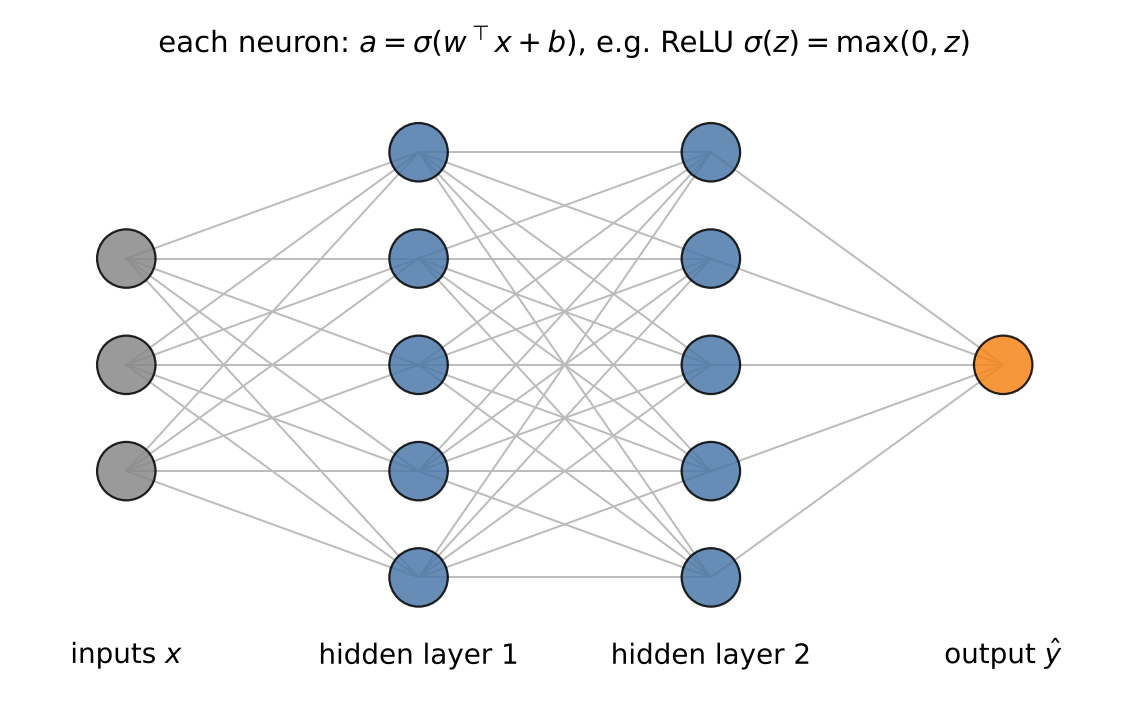
\includegraphics[width=0.8\linewidth,height=\textheight,keepaspectratio]{notebooks/images/mlp.png}

}

\caption{\label{fig-mlp}A multilayer perceptron with two hidden layers.
Each arrow carries a weight; each neuron computes a weighted sum of its
inputs and applies an activation function. Without the nonlinear
activations, the whole network would collapse into a single linear
model.}

\end{figure}%

\begin{tcolorbox}[enhanced jigsaw, colframe=quarto-callout-important-color-frame, toprule=.15mm, rightrule=.15mm, title=\textcolor{quarto-callout-important-color}{\faExclamation}\hspace{0.5em}{Universal approximation}, colbacktitle=quarto-callout-important-color!10!white, left=2mm, titlerule=0mm, bottomtitle=1mm, toptitle=1mm, opacityback=0, bottomrule=.15mm, breakable, arc=.35mm, opacitybacktitle=0.6, colback=white, coltitle=black, leftrule=.75mm]

An MLP with one hidden layer and enough neurons can approximate any
continuous function on a bounded region arbitrarily well. The theorem
guarantees that a suitable network \emph{exists} -- not that training
will find it, nor how much data is needed. In practice, deeper networks
with fewer neurons per layer often learn more efficiently.

\end{tcolorbox}

\section{Training: loss, gradients and
backpropagation}\label{training-loss-gradients-and-backpropagation}

The network's weights and biases, collected in a parameter vector
\(\theta\), are found by minimising a \textbf{loss function}
\(\mathcal{L}(\theta)\) on the training data, e.g.~the mean squared
error for regression or the cross-entropy for classification. Since the
loss is a nonconvex function of possibly millions of weights, we use
\textbf{gradient descent}:

\[\theta \leftarrow \theta - \eta\,\nabla_\theta \mathcal{L}(\theta),\]

with the \textbf{learning rate} \(\eta\). The gradient is computed by
\textbf{backpropagation} -- the chain rule of calculus applied layer by
layer from the output back to the input. Frameworks like PyTorch do this
automatically (\emph{automatic differentiation}).

Practical ingredients:

\begin{itemize}
\tightlist
\item
  \textbf{Mini-batches:} each step uses a small random subset of the
  data (e.g.~256 examples) -- \emph{stochastic} gradient descent. One
  pass through all data is an \textbf{epoch}.
\item
  \textbf{Optimisers} like Adam adapt the step size per weight and
  usually work well with default settings.
\item
  \textbf{Scaling:} inputs should be standardised; otherwise training is
  slow or unstable.
\item
  \textbf{Validation and early stopping:} monitor the loss on a
  validation set during training and stop when it no longer improves --
  the most important protection against overfitting.
\end{itemize}

\begin{tcolorbox}[enhanced jigsaw, colframe=quarto-callout-tip-color-frame, toprule=.15mm, rightrule=.15mm, title=\textcolor{quarto-callout-tip-color}{\faLightbulb}\hspace{0.5em}{Engineering practice: when is deep learning worth it?}, colbacktitle=quarto-callout-tip-color!10!white, left=2mm, titlerule=0mm, bottomtitle=1mm, toptitle=1mm, opacityback=0, bottomrule=.15mm, breakable, arc=.35mm, opacitybacktitle=0.6, colback=white, coltitle=black, leftrule=.75mm]

\begin{itemize}
\tightlist
\item
  \textbf{Raw, high-dimensional data} (images, spectrograms, long
  signals, text): yes -- neural networks learn the features.
\item
  \textbf{Tabular data with meaningful engineered features:} usually no
  -- gradient boosting is typically as good or better, faster to train
  and easier to explain.
\item
  \textbf{Little data:} usually no, unless a \textbf{pretrained} network
  can be reused (transfer learning).
\item
  Always compare with a classical baseline and consider the costs:
  training time, hardware, expertise, explainability, certification.
\end{itemize}

\end{tcolorbox}

\section{Remaining useful life from sensor
sequences}\label{remaining-useful-life-from-sensor-sequences}

The \textbf{remaining useful life (RUL)} of a machine is the time it can
still operate before failure. Predicting it is the core of predictive
maintenance: replace parts shortly before they fail, not too early
(wasted life) and not too late (unplanned failure).

Two modelling choices are typical for RUL prediction:

\begin{itemize}
\tightlist
\item
  \textbf{Sliding windows:} the input for a prediction at cycle \(t\) is
  the sensor history of the last \(L\) cycles, an \(L \times p\) matrix
  (\(p\) sensors). Each trajectory provides many overlapping windows for
  training.
\item
  \textbf{Piecewise linear target:} early in life, degradation is not
  observable in the sensors -- a new engine with 300 remaining cycles
  looks like one with 200. The RUL target is therefore capped at a
  constant (commonly 125 cycles) and decreases linearly afterwards.
\end{itemize}

\begin{figure}[H]

\centering{

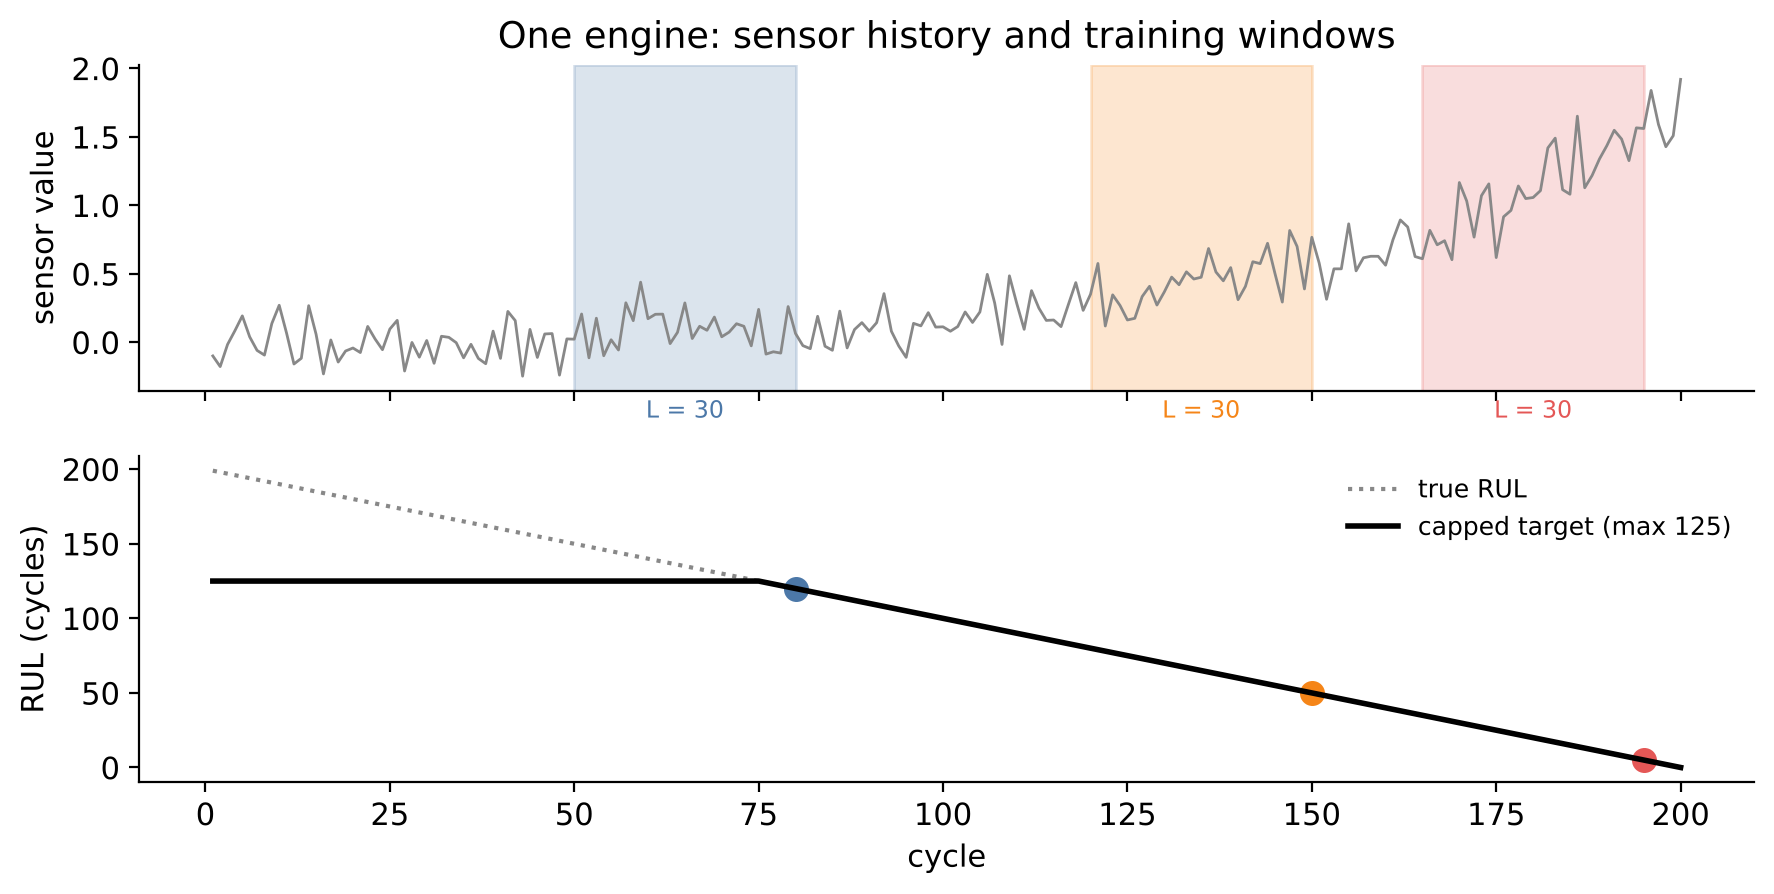
\includegraphics[width=1\linewidth,height=\textheight,keepaspectratio]{notebooks/images/rul-windows.png}

}

\caption{\label{fig-rul}Sliding windows and capped RUL target. From each
engine's sensor history, windows of L cycles are cut; the target of a
window is the RUL at its last cycle. The RUL is capped at 125 cycles
because early degradation is invisible in the data.}

\end{figure}%

Windows of the same engine are highly correlated -- exactly like signal
windows in Chapter 10. Training and validation data must be split
\textbf{by engine}.

\begin{Shaded}
\begin{Highlighting}[]
\CommentTok{\# Setup: works locally and in Google Colab}
\ImportTok{import}\NormalTok{ importlib.util, os, subprocess, sys}
\ControlFlowTok{for}\NormalTok{ pkg }\KeywordTok{in}\NormalTok{ [}\StringTok{"torch"}\NormalTok{, }\StringTok{"torchvision"}\NormalTok{]:}
    \ControlFlowTok{if}\NormalTok{ importlib.util.find\_spec(pkg) }\KeywordTok{is} \VariableTok{None}\NormalTok{:}
\NormalTok{        subprocess.run([sys.executable, }\StringTok{"{-}m"}\NormalTok{, }\StringTok{"pip"}\NormalTok{, }\StringTok{"install"}\NormalTok{, }\StringTok{"{-}q"}\NormalTok{, pkg], check}\OperatorTok{=}\VariableTok{True}\NormalTok{)}

\CommentTok{\# Windows + Anaconda: the pip build of PyTorch brings its own copy of the OpenMP runtime}
\CommentTok{\# (libiomp5md.dll), which clashes with the one used by Anaconda\textquotesingle{}s NumPy/MKL and kills the}
\CommentTok{\# kernel ("OMP: Error \#15"). This switch lets both copies coexist; it has no effect elsewhere.}
\NormalTok{os.environ.setdefault(}\StringTok{"KMP\_DUPLICATE\_LIB\_OK"}\NormalTok{, }\StringTok{"TRUE"}\NormalTok{)}

\ImportTok{import}\NormalTok{ numpy }\ImportTok{as}\NormalTok{ np}
\ImportTok{import}\NormalTok{ pandas }\ImportTok{as}\NormalTok{ pd}
\ImportTok{import}\NormalTok{ matplotlib.pyplot }\ImportTok{as}\NormalTok{ plt}
\ImportTok{import}\NormalTok{ seaborn }\ImportTok{as}\NormalTok{ sns}
\ImportTok{import}\NormalTok{ torch}
\ImportTok{from}\NormalTok{ torch }\ImportTok{import}\NormalTok{ nn}

\NormalTok{sns.set\_theme(style}\OperatorTok{=}\StringTok{"whitegrid"}\NormalTok{)}
\end{Highlighting}
\end{Shaded}

\section{Live coding: remaining useful
life}\label{live-coding-remaining-useful-life}

The data are downloaded automatically as in Chapter 3. Subset FD001 has
one operating condition and one fault mode (degradation of the
high-pressure compressor). The test file contains trajectories that end
some time \emph{before} failure; \texttt{RUL\_FD001.txt} gives the true
RUL at the end of each test trajectory.

\begin{Shaded}
\begin{Highlighting}[]
\ImportTok{from}\NormalTok{ pathlib }\ImportTok{import}\NormalTok{ Path}
\ImportTok{import}\NormalTok{ zipfile, io, requests}

\KeywordTok{def}\NormalTok{ cmapss\_dir(root}\OperatorTok{=}\NormalTok{Path(}\StringTok{"data"}\NormalTok{)):}
    \CommentTok{"""Download and extract the NASA C{-}MAPSS data once; return the folder with train\_FD001.txt."""}
\NormalTok{    root.mkdir(exist\_ok}\OperatorTok{=}\VariableTok{True}\NormalTok{)}
\NormalTok{    target }\OperatorTok{=}\NormalTok{ root }\OperatorTok{/} \StringTok{"CMAPSSData"}
    \ControlFlowTok{if} \KeywordTok{not} \BuiltInTok{any}\NormalTok{(target.rglob(}\StringTok{"train\_FD001.txt"}\NormalTok{)):}
\NormalTok{        zip\_path }\OperatorTok{=}\NormalTok{ root }\OperatorTok{/} \StringTok{"CMAPSSData.zip"}
        \ControlFlowTok{if} \KeywordTok{not}\NormalTok{ zip\_path.exists():}
\NormalTok{            r }\OperatorTok{=}\NormalTok{ requests.get(}\StringTok{"https://data.nasa.gov/docs/legacy/CMAPSSData.zip"}\NormalTok{, timeout}\OperatorTok{=}\DecValTok{300}\NormalTok{)}
\NormalTok{            r.raise\_for\_status()}
\NormalTok{            zip\_path.write\_bytes(r.content)}
        \ControlFlowTok{with}\NormalTok{ zipfile.ZipFile(zip\_path) }\ImportTok{as}\NormalTok{ z:}
\NormalTok{            z.extractall(target)}
        \ControlFlowTok{for}\NormalTok{ inner }\KeywordTok{in} \BuiltInTok{list}\NormalTok{(target.rglob(}\StringTok{"*.zip"}\NormalTok{)):          }\CommentTok{\# some versions contain a nested zip}
\NormalTok{            zipfile.ZipFile(inner).extractall(inner.parent)}
    \ControlFlowTok{return} \BuiltInTok{next}\NormalTok{(target.rglob(}\StringTok{"train\_FD001.txt"}\NormalTok{)).parent}

\NormalTok{DATA }\OperatorTok{=}\NormalTok{ cmapss\_dir()}
\NormalTok{cols }\OperatorTok{=}\NormalTok{ [}\StringTok{"unit"}\NormalTok{, }\StringTok{"cycle"}\NormalTok{, }\StringTok{"op1"}\NormalTok{, }\StringTok{"op2"}\NormalTok{, }\StringTok{"op3"}\NormalTok{] }\OperatorTok{+}\NormalTok{ [}\SpecialStringTok{f"s}\SpecialCharTok{\{}\NormalTok{i}\SpecialCharTok{\}}\SpecialStringTok{"} \ControlFlowTok{for}\NormalTok{ i }\KeywordTok{in} \BuiltInTok{range}\NormalTok{(}\DecValTok{1}\NormalTok{, }\DecValTok{22}\NormalTok{)]}
\NormalTok{read }\OperatorTok{=} \KeywordTok{lambda}\NormalTok{ f: pd.read\_csv(DATA }\OperatorTok{/}\NormalTok{ f, sep}\OperatorTok{=}\VerbatimStringTok{r"\textbackslash{}s+"}\NormalTok{, header}\OperatorTok{=}\VariableTok{None}\NormalTok{, names}\OperatorTok{=}\NormalTok{cols)}

\NormalTok{train, test }\OperatorTok{=}\NormalTok{ read(}\StringTok{"train\_FD001.txt"}\NormalTok{), read(}\StringTok{"test\_FD001.txt"}\NormalTok{)}
\NormalTok{rul\_test }\OperatorTok{=}\NormalTok{ pd.read\_csv(DATA }\OperatorTok{/} \StringTok{"RUL\_FD001.txt"}\NormalTok{, header}\OperatorTok{=}\VariableTok{None}\NormalTok{).iloc[:, }\DecValTok{0}\NormalTok{].values}

\NormalTok{train[}\StringTok{"rul"}\NormalTok{] }\OperatorTok{=}\NormalTok{ (train.groupby(}\StringTok{"unit"}\NormalTok{)[}\StringTok{"cycle"}\NormalTok{].transform(}\StringTok{"max"}\NormalTok{) }\OperatorTok{{-}}\NormalTok{ train[}\StringTok{"cycle"}\NormalTok{]).clip(upper}\OperatorTok{=}\DecValTok{125}\NormalTok{)}
\NormalTok{sensors }\OperatorTok{=}\NormalTok{ [c }\ControlFlowTok{for}\NormalTok{ c }\KeywordTok{in}\NormalTok{ cols[}\DecValTok{5}\NormalTok{:] }\ControlFlowTok{if}\NormalTok{ train[c].std() }\OperatorTok{\textgreater{}} \FloatTok{1e{-}3}\NormalTok{]       }\CommentTok{\# drop constant sensors}
\NormalTok{mu, sd }\OperatorTok{=}\NormalTok{ train[sensors].mean(), train[sensors].std()}
\NormalTok{train[sensors] }\OperatorTok{=}\NormalTok{ (train[sensors] }\OperatorTok{{-}}\NormalTok{ mu) }\OperatorTok{/}\NormalTok{ sd}
\NormalTok{test[sensors] }\OperatorTok{=}\NormalTok{ (test[sensors] }\OperatorTok{{-}}\NormalTok{ mu) }\OperatorTok{/}\NormalTok{ sd}
\BuiltInTok{print}\NormalTok{(}\StringTok{"Sensors used:"}\NormalTok{, sensors)}
\end{Highlighting}
\end{Shaded}

\begin{verbatim}
Sensors used: ['s2', 's3', 's4', 's6', 's7', 's8', 's9', 's11', 's12', 's13', 's14', 's15', 's17', 's20', 's21']
\end{verbatim}

\begin{Shaded}
\begin{Highlighting}[]
\NormalTok{fig, axes }\OperatorTok{=}\NormalTok{ plt.subplots(}\DecValTok{1}\NormalTok{, }\DecValTok{3}\NormalTok{, figsize}\OperatorTok{=}\NormalTok{(}\DecValTok{15}\NormalTok{, }\FloatTok{3.5}\NormalTok{))}
\ControlFlowTok{for}\NormalTok{ ax, s }\KeywordTok{in} \BuiltInTok{zip}\NormalTok{(axes, sensors[:}\DecValTok{3}\NormalTok{]):}
    \ControlFlowTok{for}\NormalTok{ u }\KeywordTok{in}\NormalTok{ [}\DecValTok{1}\NormalTok{, }\DecValTok{2}\NormalTok{, }\DecValTok{3}\NormalTok{, }\DecValTok{4}\NormalTok{, }\DecValTok{5}\NormalTok{]:}
\NormalTok{        g }\OperatorTok{=}\NormalTok{ train[train.unit }\OperatorTok{==}\NormalTok{ u]}
\NormalTok{        ax.plot(g[}\StringTok{"cycle"}\NormalTok{] }\OperatorTok{{-}}\NormalTok{ g[}\StringTok{"cycle"}\NormalTok{].}\BuiltInTok{max}\NormalTok{(), g[s], lw}\OperatorTok{=}\FloatTok{0.8}\NormalTok{)}
\NormalTok{    ax.}\BuiltInTok{set}\NormalTok{(title}\OperatorTok{=}\NormalTok{s, xlabel}\OperatorTok{=}\StringTok{"Cycles before failure"}\NormalTok{, ylabel}\OperatorTok{=}\StringTok{"standardised value"}\NormalTok{)}
\NormalTok{plt.tight\_layout()}\OperatorTok{;}\NormalTok{ plt.show()}
\end{Highlighting}
\end{Shaded}

\pandocbounded{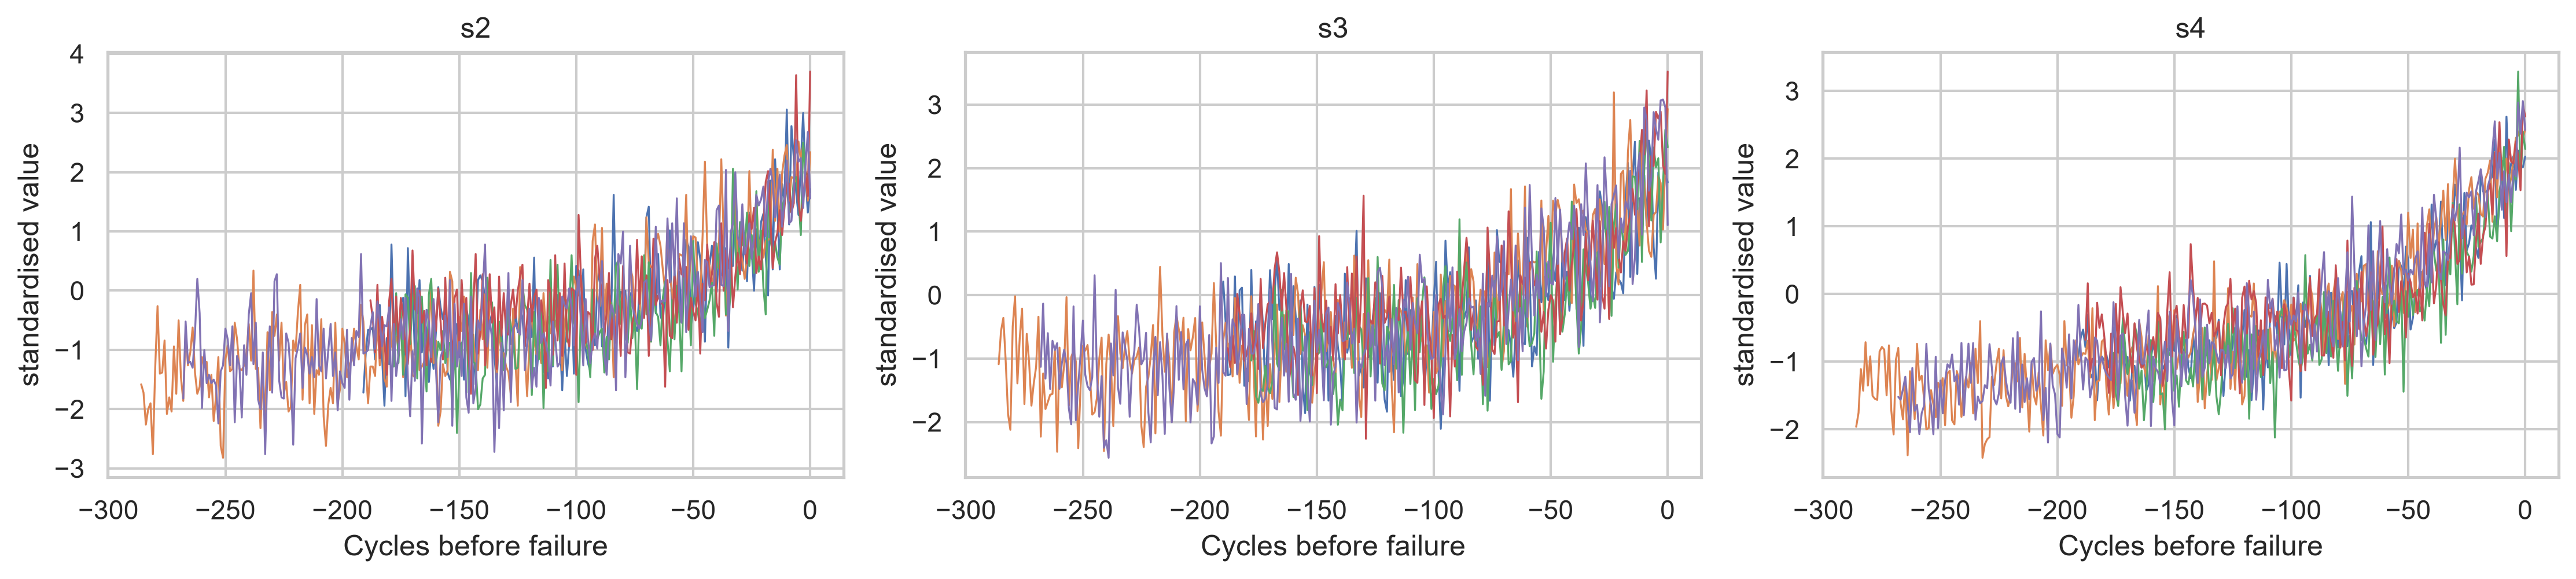
\includegraphics[keepaspectratio]{notebooks/12-neural-networks_files/figure-pdf/cell-4-output-1.png}}

Plotted against the cycles \emph{before failure}, several sensors show a
clear trend that accelerates towards the end of life -- the degradation
signature the network must learn. Some sensors are constant in FD001 and
were removed.

\begin{Shaded}
\begin{Highlighting}[]
\NormalTok{L }\OperatorTok{=} \DecValTok{30}   \CommentTok{\# window length (cycles)}

\KeywordTok{def}\NormalTok{ windows(df, with\_target}\OperatorTok{=}\VariableTok{True}\NormalTok{):}
\NormalTok{    X, y }\OperatorTok{=}\NormalTok{ [], []}
    \ControlFlowTok{for}\NormalTok{ \_, g }\KeywordTok{in}\NormalTok{ df.groupby(}\StringTok{"unit"}\NormalTok{):}
\NormalTok{        v }\OperatorTok{=}\NormalTok{ g[sensors].values}
        \ControlFlowTok{if} \BuiltInTok{len}\NormalTok{(v) }\OperatorTok{\textless{}}\NormalTok{ L:                                   }\CommentTok{\# pad short test series}
\NormalTok{            v }\OperatorTok{=}\NormalTok{ np.vstack([np.repeat(v[:}\DecValTok{1}\NormalTok{], L }\OperatorTok{{-}} \BuiltInTok{len}\NormalTok{(v), axis}\OperatorTok{=}\DecValTok{0}\NormalTok{), v])}
        \ControlFlowTok{if}\NormalTok{ with\_target:}
\NormalTok{            r }\OperatorTok{=}\NormalTok{ g[}\StringTok{"rul"}\NormalTok{].values}
            \ControlFlowTok{for}\NormalTok{ end }\KeywordTok{in} \BuiltInTok{range}\NormalTok{(L, }\BuiltInTok{len}\NormalTok{(v) }\OperatorTok{+} \DecValTok{1}\NormalTok{):}
\NormalTok{                X.append(v[end }\OperatorTok{{-}}\NormalTok{ L:end])}\OperatorTok{;}\NormalTok{ y.append(r[end }\OperatorTok{{-}} \DecValTok{1}\NormalTok{])}
        \ControlFlowTok{else}\NormalTok{:}
\NormalTok{            X.append(v[}\OperatorTok{{-}}\NormalTok{L:])}
    \ControlFlowTok{return}\NormalTok{ np.array(X, dtype}\OperatorTok{=}\NormalTok{np.float32), np.array(y, dtype}\OperatorTok{=}\NormalTok{np.float32)}

\NormalTok{X\_tr, y\_tr }\OperatorTok{=}\NormalTok{ windows(train)}
\NormalTok{X\_te, \_ }\OperatorTok{=}\NormalTok{ windows(test, with\_target}\OperatorTok{=}\VariableTok{False}\NormalTok{)}
\NormalTok{X\_tr.shape, X\_te.shape}
\end{Highlighting}
\end{Shaded}

\begin{verbatim}
((17731, 30, 15), (100, 30, 15))
\end{verbatim}

\begin{Shaded}
\begin{Highlighting}[]
\NormalTok{torch.manual\_seed(}\DecValTok{0}\NormalTok{)}
\NormalTok{model }\OperatorTok{=}\NormalTok{ nn.Sequential(}
\NormalTok{    nn.Flatten(),}
\NormalTok{    nn.Linear(L }\OperatorTok{*} \BuiltInTok{len}\NormalTok{(sensors), }\DecValTok{64}\NormalTok{), nn.ReLU(),}
\NormalTok{    nn.Linear(}\DecValTok{64}\NormalTok{, }\DecValTok{32}\NormalTok{), nn.ReLU(),}
\NormalTok{    nn.Linear(}\DecValTok{32}\NormalTok{, }\DecValTok{1}\NormalTok{),}
\NormalTok{)}
\NormalTok{opt }\OperatorTok{=}\NormalTok{ torch.optim.Adam(model.parameters(), lr}\OperatorTok{=}\FloatTok{1e{-}3}\NormalTok{)}
\NormalTok{loss\_fn }\OperatorTok{=}\NormalTok{ nn.MSELoss()}

\NormalTok{Xt, yt }\OperatorTok{=}\NormalTok{ torch.tensor(X\_tr), torch.tensor(y\_tr).unsqueeze(}\DecValTok{1}\NormalTok{)}
\NormalTok{loader }\OperatorTok{=}\NormalTok{ torch.utils.data.DataLoader(torch.utils.data.TensorDataset(Xt, yt),}
\NormalTok{                                     batch\_size}\OperatorTok{=}\DecValTok{256}\NormalTok{, shuffle}\OperatorTok{=}\VariableTok{True}\NormalTok{)}
\NormalTok{history }\OperatorTok{=}\NormalTok{ []}
\ControlFlowTok{for}\NormalTok{ epoch }\KeywordTok{in} \BuiltInTok{range}\NormalTok{(}\DecValTok{30}\NormalTok{):}
\NormalTok{    model.train()}
\NormalTok{    epoch\_loss }\OperatorTok{=} \FloatTok{0.0}
    \ControlFlowTok{for}\NormalTok{ xb, yb }\KeywordTok{in}\NormalTok{ loader:}
\NormalTok{        opt.zero\_grad()}
\NormalTok{        loss }\OperatorTok{=}\NormalTok{ loss\_fn(model(xb), yb)}
\NormalTok{        loss.backward()}
\NormalTok{        opt.step()}
\NormalTok{        epoch\_loss }\OperatorTok{+=}\NormalTok{ loss.item() }\OperatorTok{*} \BuiltInTok{len}\NormalTok{(xb)}
\NormalTok{    history.append(epoch\_loss }\OperatorTok{/} \BuiltInTok{len}\NormalTok{(Xt))}

\NormalTok{model.}\BuiltInTok{eval}\NormalTok{()}
\ControlFlowTok{with}\NormalTok{ torch.no\_grad():}
\NormalTok{    pred }\OperatorTok{=}\NormalTok{ model(torch.tensor(X\_te)).squeeze().numpy()}
\NormalTok{rmse }\OperatorTok{=}\NormalTok{ np.sqrt(np.mean((pred }\OperatorTok{{-}}\NormalTok{ np.minimum(rul\_test, }\DecValTok{125}\NormalTok{))}\OperatorTok{**}\DecValTok{2}\NormalTok{))}
\BuiltInTok{print}\NormalTok{(}\SpecialStringTok{f"Test RMSE: }\SpecialCharTok{\{}\NormalTok{rmse}\SpecialCharTok{:.1f\}}\SpecialStringTok{ cycles"}\NormalTok{)}
\end{Highlighting}
\end{Shaded}

\begin{verbatim}
Test RMSE: 15.2 cycles
\end{verbatim}

The training loop is the same in every PyTorch project: forward pass,
loss, \texttt{backward()} to compute gradients, \texttt{step()} to
update the weights. The network has a few tens of thousands of weights
-- small by deep learning standards.

\begin{Shaded}
\begin{Highlighting}[]
\NormalTok{fig, axes }\OperatorTok{=}\NormalTok{ plt.subplots(}\DecValTok{1}\NormalTok{, }\DecValTok{2}\NormalTok{, figsize}\OperatorTok{=}\NormalTok{(}\DecValTok{11}\NormalTok{, }\DecValTok{4}\NormalTok{))}
\NormalTok{axes[}\DecValTok{0}\NormalTok{].plot(history)}\OperatorTok{;}\NormalTok{ axes[}\DecValTok{0}\NormalTok{].}\BuiltInTok{set}\NormalTok{(xlabel}\OperatorTok{=}\StringTok{"Epoch"}\NormalTok{, ylabel}\OperatorTok{=}\StringTok{"Training loss (MSE)"}\NormalTok{, yscale}\OperatorTok{=}\StringTok{"log"}\NormalTok{)}
\NormalTok{axes[}\DecValTok{1}\NormalTok{].scatter(np.minimum(rul\_test, }\DecValTok{125}\NormalTok{), pred, s}\OperatorTok{=}\DecValTok{12}\NormalTok{)}
\NormalTok{axes[}\DecValTok{1}\NormalTok{].plot([}\DecValTok{0}\NormalTok{, }\DecValTok{125}\NormalTok{], [}\DecValTok{0}\NormalTok{, }\DecValTok{125}\NormalTok{], }\StringTok{"k{-}{-}"}\NormalTok{)}
\NormalTok{axes[}\DecValTok{1}\NormalTok{].}\BuiltInTok{set}\NormalTok{(xlabel}\OperatorTok{=}\StringTok{"True RUL (cycles, capped)"}\NormalTok{, ylabel}\OperatorTok{=}\StringTok{"Predicted RUL (cycles)"}\NormalTok{)}
\NormalTok{plt.tight\_layout()}\OperatorTok{;}\NormalTok{ plt.show()}
\end{Highlighting}
\end{Shaded}

\pandocbounded{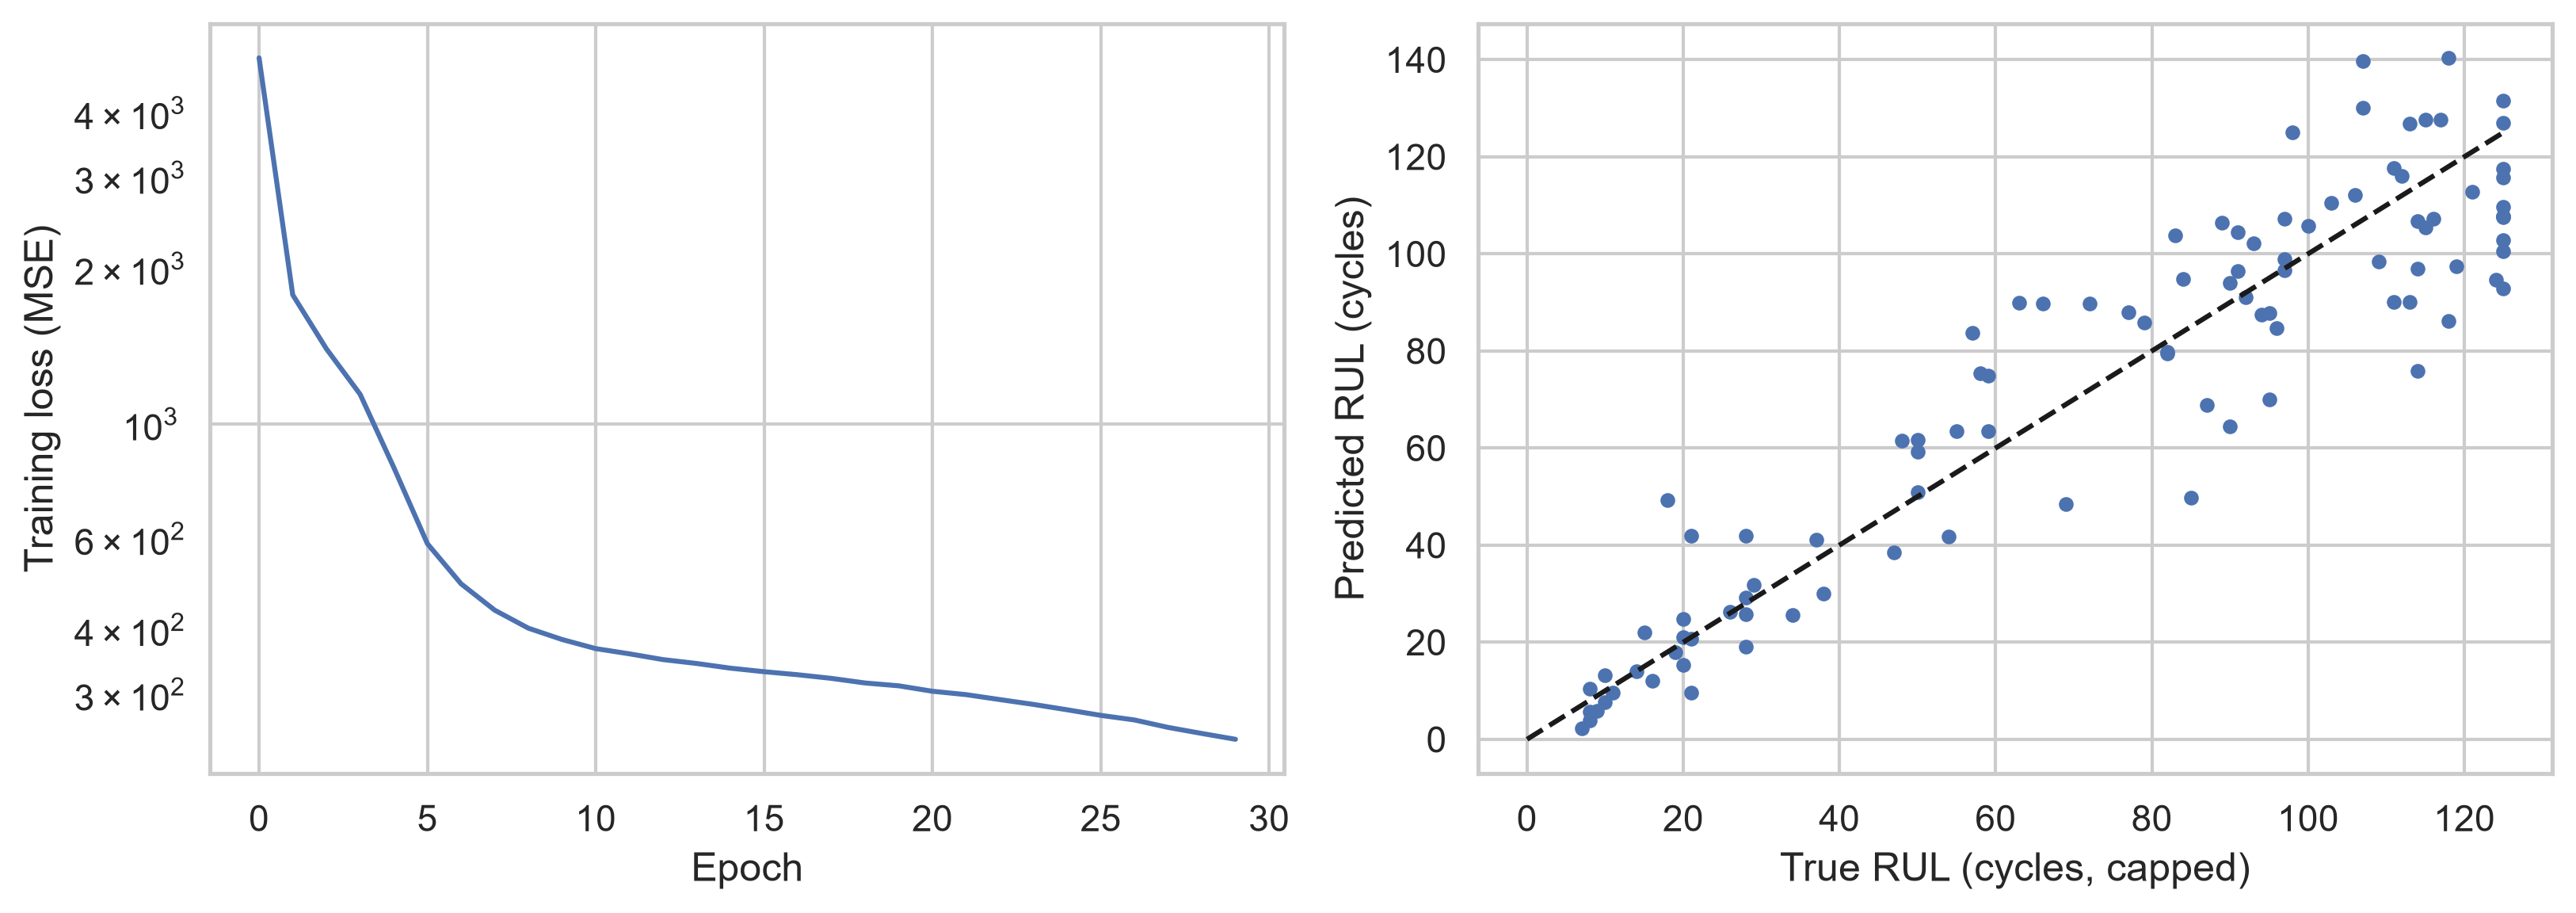
\includegraphics[keepaspectratio]{notebooks/12-neural-networks_files/figure-pdf/cell-7-output-1.png}}

\textbf{Discussion.} The predictions follow the diagonal, with larger
scatter at high RUL, where degradation is barely visible, and smaller
scatter near the end of life -- fortunately the region where accurate
predictions matter most. The training loss alone says nothing about
overfitting; we did not use a validation set here (Exercise 2 fixes
this). Also note that the test RMSE is computed on only 100 engines and
therefore has considerable uncertainty itself. Whether the network beats
a gradient boosting model on window statistics is an open question --
Exercise 1.

\section{Back to the decision}\label{back-to-the-decision-11}

An engine is scheduled too late if the model \textbf{overestimates} its
RUL. If we schedule an overhaul when \emph{predicted RUL − margin} falls
below the planning horizon, the margin must cover the overestimates of
95 \% of the engines -- i.e.~it must equal the 95 \% quantile of the
prediction error \(\hat y - y\) on the test engines.

\begin{Shaded}
\begin{Highlighting}[]
\NormalTok{true\_rul }\OperatorTok{=}\NormalTok{ np.minimum(rul\_test, }\DecValTok{125}\NormalTok{)}
\NormalTok{err }\OperatorTok{=}\NormalTok{ pred }\OperatorTok{{-}}\NormalTok{ true\_rul                                   }\CommentTok{\# \textgreater{} 0: overestimate (dangerous)}
\NormalTok{margin }\OperatorTok{=} \BuiltInTok{max}\NormalTok{(}\FloatTok{0.0}\NormalTok{, }\BuiltInTok{float}\NormalTok{(np.quantile(err, }\FloatTok{0.95}\NormalTok{)))}
\BuiltInTok{print}\NormalTok{(}\SpecialStringTok{f"Overestimated engines: }\SpecialCharTok{\{}\NormalTok{(err }\OperatorTok{\textgreater{}} \DecValTok{0}\NormalTok{)}\SpecialCharTok{.}\NormalTok{mean()}\SpecialCharTok{:.0\%\}}\SpecialStringTok{, 95 \% quantile of the error: }\SpecialCharTok{\{}\NormalTok{np}\SpecialCharTok{.}\NormalTok{quantile(err, }\FloatTok{0.95}\NormalTok{)}\SpecialCharTok{:.1f\}}\SpecialStringTok{ cycles"}\NormalTok{)}
\BuiltInTok{print}\NormalTok{(}\SpecialStringTok{f"Decision: schedule an overhaul when the predicted RUL falls below 20 + }\SpecialCharTok{\{}\NormalTok{margin}\SpecialCharTok{:.0f\}}\SpecialStringTok{ = }\SpecialCharTok{\{}\DecValTok{20} \OperatorTok{+}\NormalTok{ margin}\SpecialCharTok{:.0f\}}\SpecialStringTok{ cycles."}\NormalTok{)}
\end{Highlighting}
\end{Shaded}

\begin{verbatim}
Overestimated engines: 50%, 95 % quantile of the error: 23.9 cycles
Decision: schedule an overhaul when the predicted RUL falls below 20 + 24 = 44 cycles.
\end{verbatim}

The margin is the price of the model's uncertainty: the more accurate
the model, the smaller the margin and the more useful life is used. Note
that the quantile is estimated from only 100 test engines -- the fleet
manager should add a reserve and refine the margin with field
experience. And as in Chapter 3: C-MAPSS is a simulation, so the
procedure must be validated on real engine data before it replaces the
fixed interval.

\section{Extension: CNNs and transfer learning for visual
inspection}\label{extension-cnns-and-transfer-learning-for-visual-inspection}

\emph{Extension -- optional material, not required for the exam.}

\textbf{Convolutional neural networks (CNNs)} process images with small
learnable filters (e.g.~3 × 3 pixels) that slide across the image. Early
layers detect edges and simple textures, deeper layers combine them into
complex patterns. Because the same filter is applied everywhere, CNNs
need far fewer weights than an MLP on raw pixels.

Training a CNN from scratch requires many thousands of labelled images.
\textbf{Transfer learning} avoids this: a network pretrained on millions
of everyday images (ImageNet) already provides general visual features
that transfer surprisingly well to industrial images. For anomaly
detection, a simple but strong approach is: embed all good training
images with the pretrained CNN and score a test image by its distance to
the nearest good image in this feature space. No defective images are
needed for training.

\subsection{Live coding: anomaly detection on one MVTec
category}\label{live-coding-anomaly-detection-on-one-mvtec-category}

\textbf{Data access.} MVTec AD is free for non-commercial use (CC
BY-NC-SA 4.0) and is downloaded from the MVTec website after accepting
the license. Download one category (e.g.~\texttt{bottle}, a few hundred
MB) and extract it to \texttt{data/mvtec/bottle/}. A GPU (Colab:
\emph{Runtime → Change runtime type}) speeds things up but is not
required. Because of the manual download, the two MVTec cells are
\textbf{not executed} when the script is built -- run them yourself
after downloading the data.

\begin{Shaded}
\begin{Highlighting}[]
\ImportTok{from}\NormalTok{ pathlib }\ImportTok{import}\NormalTok{ Path}
\ImportTok{from}\NormalTok{ torchvision }\ImportTok{import}\NormalTok{ models}
\ImportTok{from}\NormalTok{ PIL }\ImportTok{import}\NormalTok{ Image}

\NormalTok{ROOT }\OperatorTok{=}\NormalTok{ Path(}\StringTok{"data/mvtec/bottle"}\NormalTok{)}
\NormalTok{device }\OperatorTok{=} \StringTok{"cuda"} \ControlFlowTok{if}\NormalTok{ torch.cuda.is\_available() }\ControlFlowTok{else} \StringTok{"cpu"}

\NormalTok{weights }\OperatorTok{=}\NormalTok{ models.ResNet18\_Weights.DEFAULT}
\NormalTok{backbone }\OperatorTok{=}\NormalTok{ models.resnet18(weights}\OperatorTok{=}\NormalTok{weights)}
\NormalTok{backbone.fc }\OperatorTok{=}\NormalTok{ torch.nn.Identity()           }\CommentTok{\# use the 512{-}d feature vector}
\NormalTok{backbone.}\BuiltInTok{eval}\NormalTok{().to(device)}
\NormalTok{tf }\OperatorTok{=}\NormalTok{ weights.transforms()}

\AttributeTok{@torch.no\_grad}\NormalTok{()}
\KeywordTok{def}\NormalTok{ embed(paths):}
\NormalTok{    feats }\OperatorTok{=}\NormalTok{ []}
    \ControlFlowTok{for}\NormalTok{ p }\KeywordTok{in}\NormalTok{ paths:}
\NormalTok{        x }\OperatorTok{=}\NormalTok{ tf(Image.}\BuiltInTok{open}\NormalTok{(p).convert(}\StringTok{"RGB"}\NormalTok{)).unsqueeze(}\DecValTok{0}\NormalTok{).to(device)}
\NormalTok{        feats.append(backbone(x).cpu().numpy()[}\DecValTok{0}\NormalTok{])}
    \ControlFlowTok{return}\NormalTok{ np.array(feats)}

\NormalTok{train\_paths }\OperatorTok{=} \BuiltInTok{sorted}\NormalTok{((ROOT }\OperatorTok{/} \StringTok{"train"} \OperatorTok{/} \StringTok{"good"}\NormalTok{).glob(}\StringTok{"*.png"}\NormalTok{))}
\NormalTok{test\_paths }\OperatorTok{=} \BuiltInTok{sorted}\NormalTok{((ROOT }\OperatorTok{/} \StringTok{"test"}\NormalTok{).glob(}\StringTok{"*/*.png"}\NormalTok{))}
\NormalTok{labels }\OperatorTok{=}\NormalTok{ np.array([p.parent.name }\OperatorTok{!=} \StringTok{"good"} \ControlFlowTok{for}\NormalTok{ p }\KeywordTok{in}\NormalTok{ test\_paths])}
\NormalTok{F\_train, F\_test }\OperatorTok{=}\NormalTok{ embed(train\_paths), embed(test\_paths)}
\end{Highlighting}
\end{Shaded}

\begin{Shaded}
\begin{Highlighting}[]
\ImportTok{from}\NormalTok{ sklearn.neighbors }\ImportTok{import}\NormalTok{ NearestNeighbors}
\ImportTok{from}\NormalTok{ sklearn.metrics }\ImportTok{import}\NormalTok{ roc\_auc\_score}

\NormalTok{nn\_model }\OperatorTok{=}\NormalTok{ NearestNeighbors(n\_neighbors}\OperatorTok{=}\DecValTok{1}\NormalTok{).fit(F\_train)}
\NormalTok{score }\OperatorTok{=}\NormalTok{ nn\_model.kneighbors(F\_test)[}\DecValTok{0}\NormalTok{][:, }\DecValTok{0}\NormalTok{]}
\BuiltInTok{print}\NormalTok{(}\SpecialStringTok{f"Image{-}level ROC AUC: }\SpecialCharTok{\{}\NormalTok{roc\_auc\_score(labels, score)}\SpecialCharTok{:.3f\}}\SpecialStringTok{"}\NormalTok{)}

\NormalTok{order }\OperatorTok{=}\NormalTok{ np.argsort(score)[::}\OperatorTok{{-}}\DecValTok{1}\NormalTok{][:}\DecValTok{5}\NormalTok{]}
\NormalTok{fig, axes }\OperatorTok{=}\NormalTok{ plt.subplots(}\DecValTok{1}\NormalTok{, }\DecValTok{5}\NormalTok{, figsize}\OperatorTok{=}\NormalTok{(}\DecValTok{15}\NormalTok{, }\DecValTok{3}\NormalTok{))}
\ControlFlowTok{for}\NormalTok{ ax, i }\KeywordTok{in} \BuiltInTok{zip}\NormalTok{(axes, order):}
\NormalTok{    ax.imshow(Image.}\BuiltInTok{open}\NormalTok{(test\_paths[i]))}\OperatorTok{;}\NormalTok{ ax.axis(}\StringTok{"off"}\NormalTok{)}
\NormalTok{    ax.set\_title(}\SpecialStringTok{f"}\SpecialCharTok{\{}\NormalTok{test\_paths[i]}\SpecialCharTok{.}\NormalTok{parent}\SpecialCharTok{.}\NormalTok{name}\SpecialCharTok{\}}\CharTok{\textbackslash{}n}\SpecialStringTok{score }\SpecialCharTok{\{}\NormalTok{score[i]}\SpecialCharTok{:.1f\}}\SpecialStringTok{"}\NormalTok{)}
\NormalTok{plt.show()}
\end{Highlighting}
\end{Shaded}

The five most anomalous test images should mostly be defective bottles.
State-of-the-art methods (e.g.~PatchCore) refine this idea by comparing
local image patches instead of whole images, which also localises the
defect.

\section{Outlook}\label{outlook}

\begin{itemize}
\tightlist
\item
  \textbf{Physics-informed machine learning:} physical laws enter the
  model as constraints or as terms of the loss function -- useful when
  data are scarce and extrapolation matters.
\item
  \textbf{Surrogate models:} neural networks or Gaussian processes
  replace expensive FEM or CFD simulations in optimisation loops.
\item
  \textbf{Foundation models:} large pretrained models for time series,
  images and text, adapted to specific tasks with little data; large
  language models as assistants for coding and documentation.
\item
  \textbf{Deployment and MLOps:} models in production must be monitored
  for \emph{data drift} (the input data change, e.g.~a new sensor or a
  new product), retrained, versioned and -- in safety-relevant
  applications -- validated and certified.
\end{itemize}

\begin{tcolorbox}[enhanced jigsaw, colframe=quarto-callout-important-color-frame, toprule=.15mm, rightrule=.15mm, title=\textcolor{quarto-callout-important-color}{\faExclamation}\hspace{0.5em}{Key takeaways}, colbacktitle=quarto-callout-important-color!10!white, left=2mm, titlerule=0mm, bottomtitle=1mm, toptitle=1mm, opacityback=0, bottomrule=.15mm, breakable, arc=.35mm, opacitybacktitle=0.6, colback=white, coltitle=black, leftrule=.75mm]

\begin{itemize}
\tightlist
\item
  A neural network is a stack of linear maps and nonlinear activations,
  trained by gradient descent with backpropagation.
\item
  Monitor a validation set and stop early; split by unit (engine,
  machine), not by window.
\item
  For RUL prediction, sliding windows and a capped target are standard;
  errors near end of life matter most.
\item
  Deep learning shines on raw images, signals and text; for tabular
  features, compare with gradient boosting first.
\end{itemize}

\end{tcolorbox}

\section{Exercises}\label{exercises-11}

\begin{enumerate}
\def\labelenumi{\arabic{enumi}.}
\tightlist
\item
  Build a baseline: gradient boosting on features of each window (last
  value, mean and slope of each sensor). Is the neural network better?
\item
  Hold out 20 training engines as a validation set (split by engine, not
  by window!) and implement early stopping. Plot training and validation
  loss.
\item
  Why is an \emph{underestimate} of the RUL less critical than an
  overestimate? Design an asymmetric loss function and discuss its
  effect.
\item
  (Extension) Replace the MLP by a 1D convolutional network
  (\texttt{nn.Conv1d}). Mind the tensor shape (batch, channels, time).
\item
  (Extension) MVTec: repeat the anomaly detection for a texture category
  (e.g.~\texttt{carpet}) and an object category (e.g.~\texttt{screw}).
  Where does the method work better? Choose a threshold so that no
  defective part passes -- what fraction of good parts is rejected?
\end{enumerate}

\subsection{Solutions}\label{solutions-11}

\begin{tcolorbox}[enhanced jigsaw, colframe=quarto-callout-caution-color-frame, toprule=.15mm, rightrule=.15mm, title=\textcolor{quarto-callout-caution-color}{\faFire}\hspace{0.5em}{Solution to Exercise 1}, colbacktitle=quarto-callout-caution-color!10!white, left=2mm, titlerule=0mm, bottomtitle=1mm, toptitle=1mm, opacityback=0, bottomrule=.15mm, breakable, arc=.35mm, opacitybacktitle=0.6, colback=white, coltitle=black, leftrule=.75mm]

\begin{Shaded}
\begin{Highlighting}[]
\ImportTok{from}\NormalTok{ sklearn.ensemble }\ImportTok{import}\NormalTok{ HistGradientBoostingRegressor}

\KeywordTok{def}\NormalTok{ window\_features(Xw):}
\NormalTok{    t }\OperatorTok{=}\NormalTok{ np.arange(L) }\OperatorTok{{-}}\NormalTok{ (L }\OperatorTok{{-}} \DecValTok{1}\NormalTok{) }\OperatorTok{/} \DecValTok{2}
\NormalTok{    slope }\OperatorTok{=}\NormalTok{ (Xw }\OperatorTok{*}\NormalTok{ t[}\VariableTok{None}\NormalTok{, :, }\VariableTok{None}\NormalTok{]).}\BuiltInTok{sum}\NormalTok{(axis}\OperatorTok{=}\DecValTok{1}\NormalTok{) }\OperatorTok{/}\NormalTok{ (t}\OperatorTok{**}\DecValTok{2}\NormalTok{).}\BuiltInTok{sum}\NormalTok{()}
    \ControlFlowTok{return}\NormalTok{ np.hstack([Xw[:, }\OperatorTok{{-}}\DecValTok{1}\NormalTok{, :], Xw.mean(axis}\OperatorTok{=}\DecValTok{1}\NormalTok{), slope])}

\NormalTok{gb }\OperatorTok{=}\NormalTok{ HistGradientBoostingRegressor(random\_state}\OperatorTok{=}\DecValTok{0}\NormalTok{).fit(window\_features(X\_tr), y\_tr)}
\NormalTok{pred\_gb }\OperatorTok{=}\NormalTok{ gb.predict(window\_features(X\_te))}
\NormalTok{rmse\_gb }\OperatorTok{=}\NormalTok{ np.sqrt(np.mean((pred\_gb }\OperatorTok{{-}}\NormalTok{ np.minimum(rul\_test, }\DecValTok{125}\NormalTok{))}\OperatorTok{**}\DecValTok{2}\NormalTok{))}
\BuiltInTok{print}\NormalTok{(}\SpecialStringTok{f"Test RMSE: MLP }\SpecialCharTok{\{}\NormalTok{rmse}\SpecialCharTok{:.1f\}}\SpecialStringTok{ cycles, gradient boosting }\SpecialCharTok{\{}\NormalTok{rmse\_gb}\SpecialCharTok{:.1f\}}\SpecialStringTok{ cycles"}\NormalTok{)}
\end{Highlighting}
\end{Shaded}

\begin{verbatim}
Test RMSE: MLP 15.2 cycles, gradient boosting 12.5 cycles
\end{verbatim}

With well-chosen window features (level, mean and trend per sensor),
gradient boosting is often on par with a small MLP on FD001 -- a
reminder that deep learning is not automatically better on sensor data
with few channels. Neural networks gain an advantage on the more complex
subsets (FD002/FD004 with six operating conditions) and with
architectures that exploit the sequence structure, such as 1D CNNs or
LSTMs.

\end{tcolorbox}

\begin{tcolorbox}[enhanced jigsaw, colframe=quarto-callout-caution-color-frame, toprule=.15mm, rightrule=.15mm, title=\textcolor{quarto-callout-caution-color}{\faFire}\hspace{0.5em}{Solution to Exercise 2}, colbacktitle=quarto-callout-caution-color!10!white, left=2mm, titlerule=0mm, bottomtitle=1mm, toptitle=1mm, opacityback=0, bottomrule=.15mm, breakable, arc=.35mm, opacitybacktitle=0.6, colback=white, coltitle=black, leftrule=.75mm]

\begin{Shaded}
\begin{Highlighting}[]
\NormalTok{rng }\OperatorTok{=}\NormalTok{ np.random.default\_rng(}\DecValTok{0}\NormalTok{)}
\NormalTok{val\_units }\OperatorTok{=}\NormalTok{ rng.choice(train[}\StringTok{"unit"}\NormalTok{].unique(), size}\OperatorTok{=}\DecValTok{20}\NormalTok{, replace}\OperatorTok{=}\VariableTok{False}\NormalTok{)}
\NormalTok{Xa, ya }\OperatorTok{=}\NormalTok{ windows(train[}\OperatorTok{\textasciitilde{}}\NormalTok{train.unit.isin(val\_units)])}
\NormalTok{Xv, yv }\OperatorTok{=}\NormalTok{ windows(train[train.unit.isin(val\_units)])}
\NormalTok{Xa\_t, ya\_t }\OperatorTok{=}\NormalTok{ torch.tensor(Xa), torch.tensor(ya).unsqueeze(}\DecValTok{1}\NormalTok{)}
\NormalTok{Xv\_t, yv\_t }\OperatorTok{=}\NormalTok{ torch.tensor(Xv), torch.tensor(yv).unsqueeze(}\DecValTok{1}\NormalTok{)}

\KeywordTok{def}\NormalTok{ make\_mlp():}
    \ControlFlowTok{return}\NormalTok{ nn.Sequential(nn.Flatten(), nn.Linear(L }\OperatorTok{*} \BuiltInTok{len}\NormalTok{(sensors), }\DecValTok{64}\NormalTok{), nn.ReLU(),}
\NormalTok{                         nn.Linear(}\DecValTok{64}\NormalTok{, }\DecValTok{32}\NormalTok{), nn.ReLU(), nn.Linear(}\DecValTok{32}\NormalTok{, }\DecValTok{1}\NormalTok{))}

\NormalTok{torch.manual\_seed(}\DecValTok{0}\NormalTok{)}
\NormalTok{net, best, best\_state, patience, wait }\OperatorTok{=}\NormalTok{ make\_mlp(), np.inf, }\VariableTok{None}\NormalTok{, }\DecValTok{5}\NormalTok{, }\DecValTok{0}
\NormalTok{opt2 }\OperatorTok{=}\NormalTok{ torch.optim.Adam(net.parameters(), lr}\OperatorTok{=}\FloatTok{1e{-}3}\NormalTok{)}
\NormalTok{dl }\OperatorTok{=}\NormalTok{ torch.utils.data.DataLoader(torch.utils.data.TensorDataset(Xa\_t, ya\_t), batch\_size}\OperatorTok{=}\DecValTok{256}\NormalTok{, shuffle}\OperatorTok{=}\VariableTok{True}\NormalTok{)}
\NormalTok{tr\_hist, va\_hist }\OperatorTok{=}\NormalTok{ [], []}
\ControlFlowTok{for}\NormalTok{ epoch }\KeywordTok{in} \BuiltInTok{range}\NormalTok{(}\DecValTok{100}\NormalTok{):}
\NormalTok{    net.train()}
    \ControlFlowTok{for}\NormalTok{ xb, yb }\KeywordTok{in}\NormalTok{ dl:}
\NormalTok{        opt2.zero\_grad()}\OperatorTok{;}\NormalTok{ l }\OperatorTok{=}\NormalTok{ loss\_fn(net(xb), yb)}\OperatorTok{;}\NormalTok{ l.backward()}\OperatorTok{;}\NormalTok{ opt2.step()}
\NormalTok{    net.}\BuiltInTok{eval}\NormalTok{()}
    \ControlFlowTok{with}\NormalTok{ torch.no\_grad():}
\NormalTok{        tr\_hist.append(loss\_fn(net(Xa\_t), ya\_t).item())}\OperatorTok{;}\NormalTok{ va\_hist.append(loss\_fn(net(Xv\_t), yv\_t).item())}
    \ControlFlowTok{if}\NormalTok{ va\_hist[}\OperatorTok{{-}}\DecValTok{1}\NormalTok{] }\OperatorTok{\textless{}}\NormalTok{ best:}
\NormalTok{        best, best\_state, wait }\OperatorTok{=}\NormalTok{ va\_hist[}\OperatorTok{{-}}\DecValTok{1}\NormalTok{], \{k: v.clone() }\ControlFlowTok{for}\NormalTok{ k, v }\KeywordTok{in}\NormalTok{ net.state\_dict().items()\}, }\DecValTok{0}
    \ControlFlowTok{else}\NormalTok{:}
\NormalTok{        wait }\OperatorTok{+=} \DecValTok{1}
        \ControlFlowTok{if}\NormalTok{ wait }\OperatorTok{\textgreater{}=}\NormalTok{ patience:}
            \ControlFlowTok{break}
\NormalTok{net.load\_state\_dict(best\_state)}
\NormalTok{plt.plot(tr\_hist, label}\OperatorTok{=}\StringTok{"training"}\NormalTok{)}\OperatorTok{;}\NormalTok{ plt.plot(va\_hist, label}\OperatorTok{=}\StringTok{"validation"}\NormalTok{)}
\NormalTok{plt.yscale(}\StringTok{"log"}\NormalTok{)}\OperatorTok{;}\NormalTok{ plt.xlabel(}\StringTok{"Epoch"}\NormalTok{)}\OperatorTok{;}\NormalTok{ plt.ylabel(}\StringTok{"MSE"}\NormalTok{)}\OperatorTok{;}\NormalTok{ plt.legend()}\OperatorTok{;}\NormalTok{ plt.show()}
\BuiltInTok{print}\NormalTok{(}\SpecialStringTok{f"stopped after }\SpecialCharTok{\{}\BuiltInTok{len}\NormalTok{(va\_hist)}\SpecialCharTok{\}}\SpecialStringTok{ epochs, best validation RMSE }\SpecialCharTok{\{}\NormalTok{np}\SpecialCharTok{.}\NormalTok{sqrt(best)}\SpecialCharTok{:.1f\}}\SpecialStringTok{ cycles"}\NormalTok{)}
\end{Highlighting}
\end{Shaded}

\pandocbounded{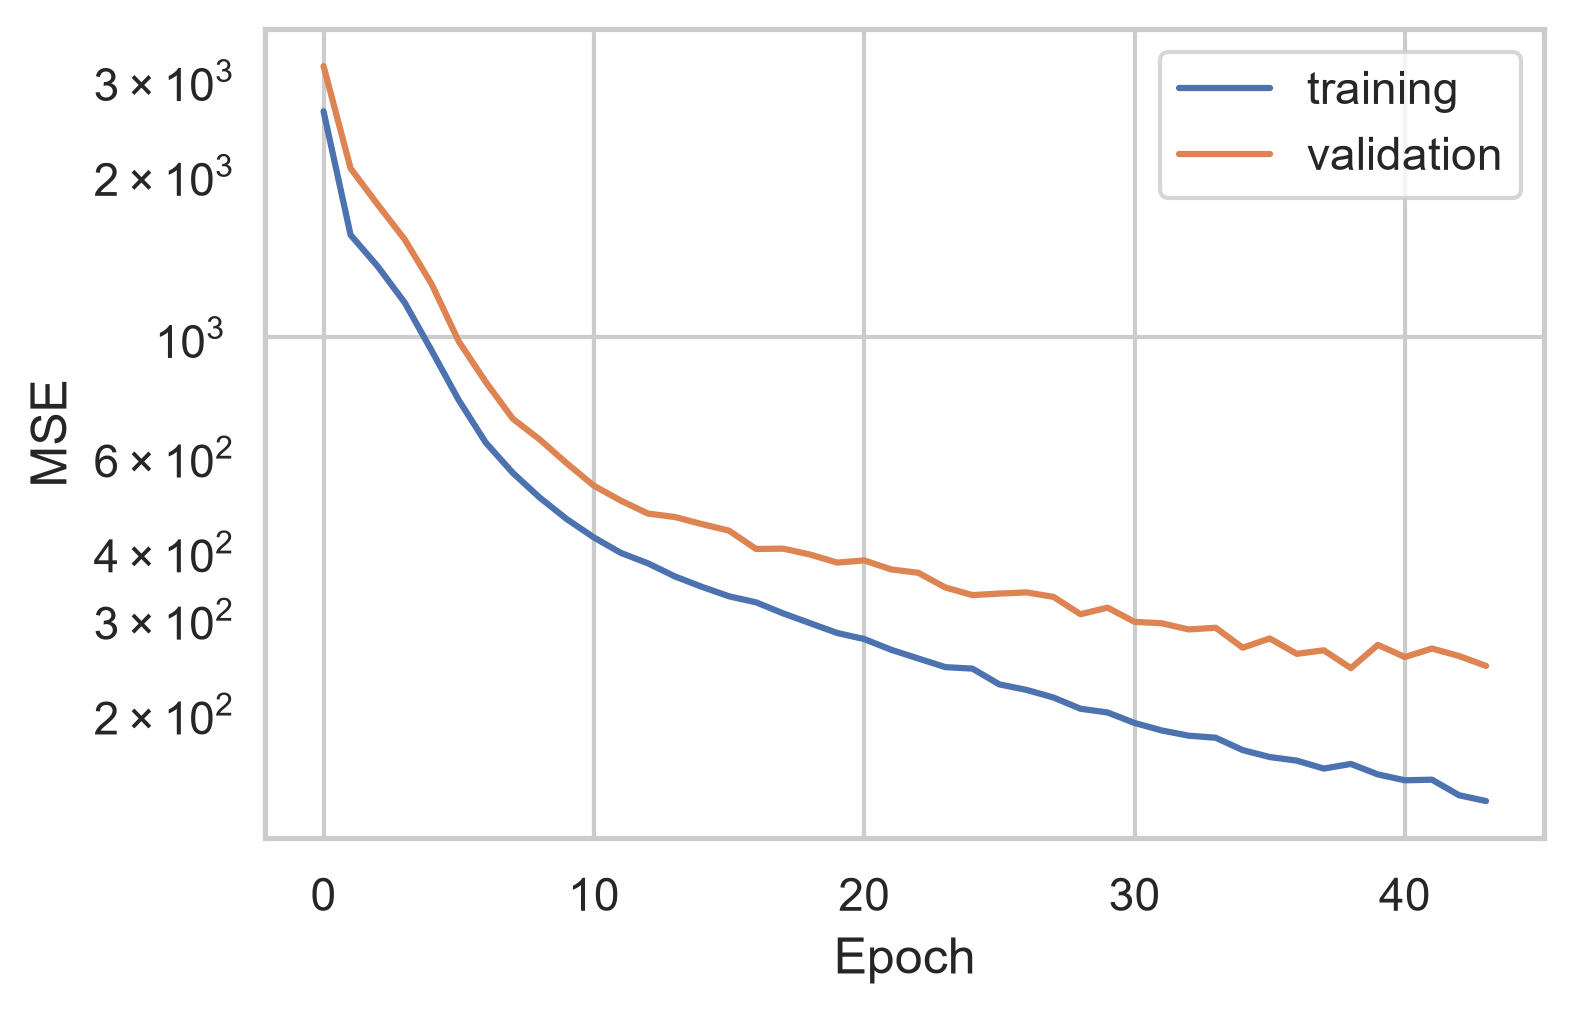
\includegraphics[keepaspectratio]{notebooks/12-neural-networks_files/figure-pdf/cell-12-output-1.png}}

\begin{verbatim}
stopped after 44 epochs, best validation RMSE 15.6 cycles
\end{verbatim}

The validation loss typically decreases at first and then flattens or
rises while the training loss keeps falling -- overfitting. Early
stopping keeps the weights of the best validation epoch. Splitting by
engine is essential: with a random window split, validation windows
would be near-copies of training windows from the same engine, and the
validation loss would keep falling.

\end{tcolorbox}

\begin{tcolorbox}[enhanced jigsaw, colframe=quarto-callout-caution-color-frame, toprule=.15mm, rightrule=.15mm, title=\textcolor{quarto-callout-caution-color}{\faFire}\hspace{0.5em}{Solution to Exercise 3}, colbacktitle=quarto-callout-caution-color!10!white, left=2mm, titlerule=0mm, bottomtitle=1mm, toptitle=1mm, opacityback=0, bottomrule=.15mm, breakable, arc=.35mm, opacitybacktitle=0.6, colback=white, coltitle=black, leftrule=.75mm]

An underestimate leads to maintenance too early: some useful life is
wasted, a cost that can be planned. An overestimate means the machine
may fail before maintenance: unplanned downtime, secondary damage,
possibly a safety risk. An asymmetric loss penalises late predictions
(predicted RUL \textgreater{} true RUL) more strongly, e.g.~the score of
the PHM 2008 challenge with \(d = \hat y - y\):
\[s(d) = \begin{cases} e^{-d/13} - 1, & d < 0 \\ e^{d/10} - 1, & d \ge 0. \end{cases}\]
A simpler differentiable variant for training is a weighted squared
error:

\begin{Shaded}
\begin{Highlighting}[]
\KeywordTok{def}\NormalTok{ asymmetric\_mse(pred, target, w\_late}\OperatorTok{=}\FloatTok{4.0}\NormalTok{):}
\NormalTok{    d }\OperatorTok{=}\NormalTok{ pred }\OperatorTok{{-}}\NormalTok{ target}
    \ControlFlowTok{return}\NormalTok{ torch.mean(torch.where(d }\OperatorTok{\textgreater{}} \DecValTok{0}\NormalTok{, w\_late }\OperatorTok{*}\NormalTok{ d}\OperatorTok{**}\DecValTok{2}\NormalTok{, d}\OperatorTok{**}\DecValTok{2}\NormalTok{))}
\end{Highlighting}
\end{Shaded}

Training with such a loss shifts the predictions towards lower RUL
values -- the model becomes deliberately conservative. The weight should
reflect the real cost ratio of late and early maintenance.

\end{tcolorbox}

\begin{tcolorbox}[enhanced jigsaw, colframe=quarto-callout-caution-color-frame, toprule=.15mm, rightrule=.15mm, title=\textcolor{quarto-callout-caution-color}{\faFire}\hspace{0.5em}{Solution to Exercise 4}, colbacktitle=quarto-callout-caution-color!10!white, left=2mm, titlerule=0mm, bottomtitle=1mm, toptitle=1mm, opacityback=0, bottomrule=.15mm, breakable, arc=.35mm, opacitybacktitle=0.6, colback=white, coltitle=black, leftrule=.75mm]

\begin{Shaded}
\begin{Highlighting}[]
\KeywordTok{class}\NormalTok{ CNN1D(nn.Module):}
    \KeywordTok{def} \FunctionTok{\_\_init\_\_}\NormalTok{(}\VariableTok{self}\NormalTok{, n\_sensors):}
        \BuiltInTok{super}\NormalTok{().}\FunctionTok{\_\_init\_\_}\NormalTok{()}
        \VariableTok{self}\NormalTok{.net }\OperatorTok{=}\NormalTok{ nn.Sequential(}
\NormalTok{            nn.Conv1d(n\_sensors, }\DecValTok{32}\NormalTok{, kernel\_size}\OperatorTok{=}\DecValTok{5}\NormalTok{, padding}\OperatorTok{=}\DecValTok{2}\NormalTok{), nn.ReLU(),}
\NormalTok{            nn.Conv1d(}\DecValTok{32}\NormalTok{, }\DecValTok{32}\NormalTok{, kernel\_size}\OperatorTok{=}\DecValTok{5}\NormalTok{, padding}\OperatorTok{=}\DecValTok{2}\NormalTok{), nn.ReLU(),}
\NormalTok{            nn.AdaptiveAvgPool1d(}\DecValTok{1}\NormalTok{), nn.Flatten(), nn.Linear(}\DecValTok{32}\NormalTok{, }\DecValTok{1}\NormalTok{))}

    \KeywordTok{def}\NormalTok{ forward(}\VariableTok{self}\NormalTok{, x):                  }\CommentTok{\# x: (batch, time, sensors)}
        \ControlFlowTok{return} \VariableTok{self}\NormalTok{.net(x.transpose(}\DecValTok{1}\NormalTok{, }\DecValTok{2}\NormalTok{))  }\CommentTok{\# Conv1d expects (batch, channels, time)}

\NormalTok{torch.manual\_seed(}\DecValTok{0}\NormalTok{)}
\NormalTok{cnn }\OperatorTok{=}\NormalTok{ CNN1D(}\BuiltInTok{len}\NormalTok{(sensors))}
\NormalTok{opt3 }\OperatorTok{=}\NormalTok{ torch.optim.Adam(cnn.parameters(), lr}\OperatorTok{=}\FloatTok{1e{-}3}\NormalTok{)}
\ControlFlowTok{for}\NormalTok{ epoch }\KeywordTok{in} \BuiltInTok{range}\NormalTok{(}\DecValTok{30}\NormalTok{):}
\NormalTok{    cnn.train()}
    \ControlFlowTok{for}\NormalTok{ xb, yb }\KeywordTok{in}\NormalTok{ loader:}
\NormalTok{        opt3.zero\_grad()}\OperatorTok{;}\NormalTok{ l }\OperatorTok{=}\NormalTok{ loss\_fn(cnn(xb), yb)}\OperatorTok{;}\NormalTok{ l.backward()}\OperatorTok{;}\NormalTok{ opt3.step()}
\NormalTok{cnn.}\BuiltInTok{eval}\NormalTok{()}
\ControlFlowTok{with}\NormalTok{ torch.no\_grad():}
\NormalTok{    pred\_cnn }\OperatorTok{=}\NormalTok{ cnn(torch.tensor(X\_te)).squeeze().numpy()}
\BuiltInTok{print}\NormalTok{(}\SpecialStringTok{f"Test RMSE 1D CNN: }\SpecialCharTok{\{}\NormalTok{np}\SpecialCharTok{.}\NormalTok{sqrt(np.mean((pred\_cnn }\OperatorTok{{-}}\NormalTok{ np.minimum(rul\_test, }\DecValTok{125}\NormalTok{))}\OperatorTok{**}\DecValTok{2}\NormalTok{))}\SpecialCharTok{:.1f\}}\SpecialStringTok{ cycles"}\NormalTok{)}
\end{Highlighting}
\end{Shaded}

\begin{verbatim}
Test RMSE 1D CNN: 18.2 cycles
\end{verbatim}

The convolution filters slide along the time axis and share their
weights over time, so the network detects local patterns (e.g.~a
steepening trend) wherever they occur in the window. The sensors are the
input \emph{channels} -- hence the transposition from (batch, time,
sensors) to (batch, sensors, time).

\end{tcolorbox}

\begin{tcolorbox}[enhanced jigsaw, colframe=quarto-callout-caution-color-frame, toprule=.15mm, rightrule=.15mm, title=\textcolor{quarto-callout-caution-color}{\faFire}\hspace{0.5em}{Solution to Exercise 5}, colbacktitle=quarto-callout-caution-color!10!white, left=2mm, titlerule=0mm, bottomtitle=1mm, toptitle=1mm, opacityback=0, bottomrule=.15mm, breakable, arc=.35mm, opacitybacktitle=0.6, colback=white, coltitle=black, leftrule=.75mm]

Change \texttt{ROOT} to the new category and rerun the two cells.
Image-level anomaly detection with global features typically works very
well for objects with consistent appearance (bottle) and for many
textures, but less well for categories with small, local defects on
objects with varying pose (screw), because a global feature vector
averages over the whole image. For a threshold that lets no defective
part pass:

\begin{Shaded}
\begin{Highlighting}[]
\NormalTok{thr }\OperatorTok{=}\NormalTok{ score[labels].}\BuiltInTok{min}\NormalTok{()                          }\CommentTok{\# lowest score among defective images}
\NormalTok{false\_reject }\OperatorTok{=}\NormalTok{ (score[}\OperatorTok{\textasciitilde{}}\NormalTok{labels] }\OperatorTok{\textgreater{}=}\NormalTok{ thr).mean()}
\BuiltInTok{print}\NormalTok{(}\SpecialStringTok{f"threshold }\SpecialCharTok{\{}\NormalTok{thr}\SpecialCharTok{:.2f\}}\SpecialStringTok{: }\SpecialCharTok{\{}\NormalTok{false\_reject}\SpecialCharTok{:.0\%\}}\SpecialStringTok{ of good parts rejected"}\NormalTok{)}
\end{Highlighting}
\end{Shaded}

The resulting false reject rate shows the price of zero slip. Note that
this threshold was chosen on the test set itself and is therefore
optimistic; in practice it must be set on separate validation images.

\end{tcolorbox}

\chapter{Review and Exam Preparation}\label{review-and-exam-preparation}

This chapter collects the methods of the course in one map, lists the
most important pitfalls and offers practice questions in the style of
the exam. The exam is written, without a computer: it tests
understanding, interpretation and method choice -- not programming
routine. Sections marked \emph{Extension} in the chapters are not part
of the exam; in the tables below they are marked (ext.).

\section{Which method when?}\label{which-method-when}

\begin{longtable}[]{@{}
  >{\raggedright\arraybackslash}p{(\linewidth - 6\tabcolsep) * \real{0.2500}}
  >{\raggedright\arraybackslash}p{(\linewidth - 6\tabcolsep) * \real{0.2500}}
  >{\raggedright\arraybackslash}p{(\linewidth - 6\tabcolsep) * \real{0.2500}}
  >{\raggedright\arraybackslash}p{(\linewidth - 6\tabcolsep) * \real{0.2500}}@{}}
\toprule\noalign{}
\begin{minipage}[b]{\linewidth}\raggedright
Engineering question
\end{minipage} & \begin{minipage}[b]{\linewidth}\raggedright
Data
\end{minipage} & \begin{minipage}[b]{\linewidth}\raggedright
Method
\end{minipage} & \begin{minipage}[b]{\linewidth}\raggedright
Chapter
\end{minipage} \\
\midrule\noalign{}
\endhead
\bottomrule\noalign{}
\endlastfoot
How reliable is a component? & lifetimes & Weibull fit, B10 life,
bootstrap & 3 \\
How much can we trust an alarm? & detection and false alarm rates, base
rate & Bayes' theorem & 3, 7 \\
Few tests, but prior knowledge & counts, earlier products & Bayesian
updating (beta--binomial) (ext.) & 3 \\
Did a change improve the process? & measurements of two or more groups &
t-test, ANOVA, effect size & 4 \\
How many samples do I need? & assumed effect and noise & power analysis
& 4 \\
How does an output depend on inputs? & continuous, few inputs & linear
regression, design of experiments (ext.) & 5 \\
Fit a physical or empirical law & measured curve & nonlinear least
squares (\texttt{curve\_fit}) & 5 \\
Predict a continuous quantity & many inputs & regularised regression,
gradient boosting & 6, 8 \\
Expensive experiments or simulations & few runs & Gaussian process,
Bayesian optimisation (ext.) & 6 \\
OK / not OK, fault type & labelled data & logistic regression, trees,
ensembles & 7, 8 \\
Why does the model decide this way? & trained model & permutation
importance, partial dependence, SHAP (ext.) & 8 \\
Detect unknown deviations & mostly normal data & PCA (T², SPE),
Isolation Forest & 9 \\
Find operating modes or groups & unlabelled data & k-means, DBSCAN &
9 \\
Diagnose rotating machinery & vibration signals & FFT, statistical
features, envelope spectrum (ext.) & 10 \\
Forecast demand or load & time series & baselines, lag features +
boosting, SARIMA (ext.) & 11 \\
Remaining useful life & multivariate sequences & neural networks,
boosting baseline & 12 \\
Inspect surfaces & images & pretrained CNN, anomaly detection (ext.) &
12 \\
\end{longtable}

\section{Core concepts at a glance}\label{core-concepts-at-a-glance}

\begin{longtable}[]{@{}
  >{\raggedright\arraybackslash}p{(\linewidth - 4\tabcolsep) * \real{0.3333}}
  >{\raggedright\arraybackslash}p{(\linewidth - 4\tabcolsep) * \real{0.3333}}
  >{\raggedright\arraybackslash}p{(\linewidth - 4\tabcolsep) * \real{0.3333}}@{}}
\toprule\noalign{}
\begin{minipage}[b]{\linewidth}\raggedright
Concept
\end{minipage} & \begin{minipage}[b]{\linewidth}\raggedright
In one sentence
\end{minipage} & \begin{minipage}[b]{\linewidth}\raggedright
Chapter
\end{minipage} \\
\midrule\noalign{}
\endhead
\bottomrule\noalign{}
\endlastfoot
CRISP-DM & Process model: understanding → data → preparation → modelling
→ evaluation → deployment, iterated. & 1 \\
Statistics vs.~ML & Statistics focuses on understanding and uncertainty,
ML on prediction for new data; they overlap in statistical learning. &
1 \\
Robust statistics & Median, IQR and MAD are barely affected by outliers,
mean and standard deviation are. & 2 \\
MCAR / MAR / MNAR & Whether missingness is random, depends on observed
data, or on the missing value itself. & 2 \\
Central limit theorem & Means of many independent observations are
approximately normal, with standard error \(\sigma/\sqrt{n}\). & 3 \\
Weibull shape \(\beta\) & \(<1\) early failures, \(=1\) random failures,
\(>1\) wear-out. & 3 \\
Confidence interval & A procedure that captures the true parameter in 95
\% of repetitions. & 3 \\
p-value & Probability of data at least as extreme as observed, assuming
\(H_0\). & 4 \\
Effect size & Size of a difference in physical units or standard
deviations; decides relevance. & 4 \\
Prediction interval & Interval for a single new observation; wider than
the confidence interval of the mean. & 5 \\
Bias--variance trade-off & Too simple models underfit, too flexible
models overfit; the test error is U-shaped. & 6 \\
Cross-validation & Estimate of the test error by rotating held-out
folds. & 6 \\
Precision / recall & Share of alarms that are real / share of failures
that are detected. & 7 \\
Bagging / boosting & Averaging decorrelated deep trees / adding shallow
trees that correct errors. & 8 \\
T² / SPE & Unusual within the PCA model plane / distance from the plane.
& 9 \\
Nyquist frequency & Half the sampling rate; higher frequencies alias. &
10 \\
Time series validation & Train on the past, test on the following
period. & 11 \\
Backpropagation & Chain rule to compute the gradient of the loss with
respect to all weights. & 12 \\
\end{longtable}

\section{Checklist: typical pitfalls}\label{checklist-typical-pitfalls}

\begin{tcolorbox}[enhanced jigsaw, colframe=quarto-callout-warning-color-frame, toprule=.15mm, rightrule=.15mm, title=\textcolor{quarto-callout-warning-color}{\faExclamationTriangle}\hspace{0.5em}{Before you trust a result, check \ldots{}}, colbacktitle=quarto-callout-warning-color!10!white, left=2mm, titlerule=0mm, bottomtitle=1mm, toptitle=1mm, opacityback=0, bottomrule=.15mm, breakable, arc=.35mm, opacitybacktitle=0.6, colback=white, coltitle=black, leftrule=.75mm]

\begin{itemize}
\tightlist
\item
  \textbf{Data leakage:} features that contain the answer, preprocessing
  fitted on all data, random splits of time series, windows or parts of
  the same unit in training and test.
\item
  \textbf{Wrong metric:} accuracy or ROC on imbalanced data; MAPE near
  zero values.
\item
  \textbf{Significance without relevance:} tiny effects with huge \(n\);
  dependent observations treated as independent.
\item
  \textbf{Extrapolation:} predictions outside the range (or the
  combinations) of the training data.
\item
  \textbf{Missing baseline:} no comparison with the mean, the seasonal
  naive forecast or a simple linear model.
\item
  \textbf{Correlation vs.~causation:} importance and correlation do not
  prove that a factor causes the effect.
\end{itemize}

\end{tcolorbox}

\section{Typical exam question types}\label{typical-exam-question-types}

\begin{enumerate}
\def\labelenumi{\arabic{enumi}.}
\tightlist
\item
  \textbf{Method choice:} given a scenario, choose and justify a method
  and an evaluation metric.
\item
  \textbf{Interpretation:} read a regression table, a confusion matrix,
  a scree plot, a probability plot or a learning curve.
\item
  \textbf{Calculation by hand:} confidence interval, test statistic,
  Bayes' theorem, precision/recall from a confusion matrix, aliasing
  frequency.
\item
  \textbf{Code reading:} find the error in a short Python snippet.
\end{enumerate}

\section{Practice questions}\label{practice-questions}

\begin{enumerate}
\def\labelenumi{\arabic{enumi}.}
\tightlist
\item
  A confusion matrix shows TN = 950, FP = 30, FN = 5, TP = 15. Compute
  accuracy, precision and recall. Is the model useful for failure
  detection?
\item
  A sensor detects 99 \% of all leaks and raises a false alarm in 2 \%
  of the leak-free tests; 0.5 \% of all parts leak. What is the
  probability that a part with an alarm really leaks?
\item
  Find the error:
  \texttt{X\ =\ StandardScaler().fit\_transform(X);\ X\_train,\ X\_test,\ y\_train,\ y\_test\ =\ train\_test\_split(X,\ y)}.
\item
  A t-test on 50,000 parts shows p \textless{} 0.001 for a 0.2 µm
  difference in mean diameter, tolerance ±20 µm. What do you tell the
  production manager?
\item
  Explain to a colleague, in five sentences, why a random train/test
  split is wrong for load forecasting.
\item
  Ten measurements of a shaft diameter give \(\bar x = 25.012\) mm and
  \(s = 0.004\) mm. Compute a 95 \% confidence interval for the mean
  diameter (\(t_{9,\,0.975} = 2.262\)).
\item
  A Weibull analysis of pump seals gives \(\beta = 0.8\). The
  maintenance manager wants to replace all seals preventively after
  2,000 hours. What do you advise?
\item
  A regression of tool wear on cutting speed gives \(R^2 = 0.95\) on the
  training data. The CV error is three times the training error. What do
  you conclude, and what do you do?
\item
  A vibration signal is sampled at 2 kHz. A gear mesh frequency of 1.6
  kHz is present. Where does it appear in the spectrum?
\item
  In a PCA monitoring chart, a new production run exceeds the SPE limit
  but not the T² limit. How do you interpret this?
\end{enumerate}

\subsection{Solutions}\label{solutions-12}

\begin{tcolorbox}[enhanced jigsaw, colframe=quarto-callout-caution-color-frame, toprule=.15mm, rightrule=.15mm, title=\textcolor{quarto-callout-caution-color}{\faFire}\hspace{0.5em}{Solution to Question 1}, colbacktitle=quarto-callout-caution-color!10!white, left=2mm, titlerule=0mm, bottomtitle=1mm, toptitle=1mm, opacityback=0, bottomrule=.15mm, breakable, arc=.35mm, opacitybacktitle=0.6, colback=white, coltitle=black, leftrule=.75mm]

Accuracy = 965/1000 = 96.5 \%, precision = 15/45 = 33 \%, recall = 15/20
= 75 \%. The trivial model ``always OK'' would reach 98 \% accuracy, so
accuracy is misleading here. The model detects three out of four
failures with two false alarms per real alarm. Whether it is useful
depends on the cost ratio of missed failures and false alarms -- often
yes.

\end{tcolorbox}

\begin{tcolorbox}[enhanced jigsaw, colframe=quarto-callout-caution-color-frame, toprule=.15mm, rightrule=.15mm, title=\textcolor{quarto-callout-caution-color}{\faFire}\hspace{0.5em}{Solution to Question 2}, colbacktitle=quarto-callout-caution-color!10!white, left=2mm, titlerule=0mm, bottomtitle=1mm, toptitle=1mm, opacityback=0, bottomrule=.15mm, breakable, arc=.35mm, opacitybacktitle=0.6, colback=white, coltitle=black, leftrule=.75mm]

\[P(\text{leak} \mid \text{alarm}) = \frac{0.99 \cdot 0.005}{0.99 \cdot 0.005 + 0.02 \cdot 0.995} = \frac{0.00495}{0.00495 + 0.0199} \approx 0.20.\]
Only about one in five alarms is a real leak -- the base rate effect.
Alarmed parts should be re-tested before scrapping.

\end{tcolorbox}

\begin{tcolorbox}[enhanced jigsaw, colframe=quarto-callout-caution-color-frame, toprule=.15mm, rightrule=.15mm, title=\textcolor{quarto-callout-caution-color}{\faFire}\hspace{0.5em}{Solution to Question 3}, colbacktitle=quarto-callout-caution-color!10!white, left=2mm, titlerule=0mm, bottomtitle=1mm, toptitle=1mm, opacityback=0, bottomrule=.15mm, breakable, arc=.35mm, opacitybacktitle=0.6, colback=white, coltitle=black, leftrule=.75mm]

The scaler is fitted on all data before the split, so means and standard
deviations of the test data leak into the preprocessing. Correct: split
first, then fit the scaler on the training data only -- best by putting
scaler and model into a \texttt{Pipeline}. (For time series,
additionally \texttt{shuffle=False} or a time-based split.)

\end{tcolorbox}

\begin{tcolorbox}[enhanced jigsaw, colframe=quarto-callout-caution-color-frame, toprule=.15mm, rightrule=.15mm, title=\textcolor{quarto-callout-caution-color}{\faFire}\hspace{0.5em}{Solution to Question 4}, colbacktitle=quarto-callout-caution-color!10!white, left=2mm, titlerule=0mm, bottomtitle=1mm, toptitle=1mm, opacityback=0, bottomrule=.15mm, breakable, arc=.35mm, opacitybacktitle=0.6, colback=white, coltitle=black, leftrule=.75mm]

The difference is statistically significant but practically irrelevant:
0.2 µm is 1 \% of the tolerance half-width. With 50,000 parts, the test
detects even tiny differences. No action is needed because of this
difference; what matters is whether the process stays within tolerance
(process capability).

\end{tcolorbox}

\begin{tcolorbox}[enhanced jigsaw, colframe=quarto-callout-caution-color-frame, toprule=.15mm, rightrule=.15mm, title=\textcolor{quarto-callout-caution-color}{\faFire}\hspace{0.5em}{Solution to Question 5}, colbacktitle=quarto-callout-caution-color!10!white, left=2mm, titlerule=0mm, bottomtitle=1mm, toptitle=1mm, opacityback=0, bottomrule=.15mm, breakable, arc=.35mm, opacitybacktitle=0.6, colback=white, coltitle=black, leftrule=.75mm]

Neighbouring hours and days are strongly correlated. With a random
split, the test days are surrounded by training days from before
\emph{and after}, so the model only interpolates. In operation, a
forecast must be made without knowing the future. The random split
therefore underestimates the real forecast error. A time-based split --
train on the past, test on the following period -- reproduces the real
situation.

\end{tcolorbox}

\begin{tcolorbox}[enhanced jigsaw, colframe=quarto-callout-caution-color-frame, toprule=.15mm, rightrule=.15mm, title=\textcolor{quarto-callout-caution-color}{\faFire}\hspace{0.5em}{Solution to Question 6}, colbacktitle=quarto-callout-caution-color!10!white, left=2mm, titlerule=0mm, bottomtitle=1mm, toptitle=1mm, opacityback=0, bottomrule=.15mm, breakable, arc=.35mm, opacitybacktitle=0.6, colback=white, coltitle=black, leftrule=.75mm]

\[25.012 \pm 2.262 \cdot \frac{0.004}{\sqrt{10}} = 25.012 \pm 0.0029\ \text{mm} \;\Rightarrow\; [25.0091,\ 25.0149]\ \text{mm}.\]
The interval describes the uncertainty of the \emph{mean} diameter, not
the spread of individual shafts (about ±2s = ±0.008 mm).

\end{tcolorbox}

\begin{tcolorbox}[enhanced jigsaw, colframe=quarto-callout-caution-color-frame, toprule=.15mm, rightrule=.15mm, title=\textcolor{quarto-callout-caution-color}{\faFire}\hspace{0.5em}{Solution to Question 7}, colbacktitle=quarto-callout-caution-color!10!white, left=2mm, titlerule=0mm, bottomtitle=1mm, toptitle=1mm, opacityback=0, bottomrule=.15mm, breakable, arc=.35mm, opacitybacktitle=0.6, colback=white, coltitle=black, leftrule=.75mm]

\(\beta < 1\) means a decreasing failure rate -- early failures dominate
(e.g.~installation errors, defective batches). A new seal is then
\emph{more} likely to fail soon than an old one, so preventive
replacement at 2,000 hours would increase the number of failures and
costs. Better: investigate the cause of the early failures
(installation, quality of supply) and possibly run-in tests.

\end{tcolorbox}

\begin{tcolorbox}[enhanced jigsaw, colframe=quarto-callout-caution-color-frame, toprule=.15mm, rightrule=.15mm, title=\textcolor{quarto-callout-caution-color}{\faFire}\hspace{0.5em}{Solution to Question 8}, colbacktitle=quarto-callout-caution-color!10!white, left=2mm, titlerule=0mm, bottomtitle=1mm, toptitle=1mm, opacityback=0, bottomrule=.15mm, breakable, arc=.35mm, opacitybacktitle=0.6, colback=white, coltitle=black, leftrule=.75mm]

The large gap between training and cross-validation error indicates
overfitting: the model is too flexible for the amount of data, and the
high training \(R^2\) is misleading. Actions: simpler model (fewer
terms, lower polynomial degree), regularisation, more data; select the
complexity by cross-validation and report the CV or test error, not the
training \(R^2\).

\end{tcolorbox}

\begin{tcolorbox}[enhanced jigsaw, colframe=quarto-callout-caution-color-frame, toprule=.15mm, rightrule=.15mm, title=\textcolor{quarto-callout-caution-color}{\faFire}\hspace{0.5em}{Solution to Question 9}, colbacktitle=quarto-callout-caution-color!10!white, left=2mm, titlerule=0mm, bottomtitle=1mm, toptitle=1mm, opacityback=0, bottomrule=.15mm, breakable, arc=.35mm, opacitybacktitle=0.6, colback=white, coltitle=black, leftrule=.75mm]

The Nyquist frequency is 1 kHz. The 1.6 kHz component aliases to
\(|1.6 - 2.0| = 0.4\) kHz = 400 Hz. The spectrum shows a false peak at
400 Hz. A sampling rate above 3.2 kHz (in practice ≥ 4 kHz) with an
anti-aliasing filter is needed.

\end{tcolorbox}

\begin{tcolorbox}[enhanced jigsaw, colframe=quarto-callout-caution-color-frame, toprule=.15mm, rightrule=.15mm, title=\textcolor{quarto-callout-caution-color}{\faFire}\hspace{0.5em}{Solution to Question 10}, colbacktitle=quarto-callout-caution-color!10!white, left=2mm, titlerule=0mm, bottomtitle=1mm, toptitle=1mm, opacityback=0, bottomrule=.15mm, breakable, arc=.35mm, opacitybacktitle=0.6, colback=white, coltitle=black, leftrule=.75mm]

A high SPE with normal T² means that the run shows a pattern of
variation that the PCA model of normal operation does not contain -- a
new kind of deviation, e.g.~a sensor fault, a broken correlation between
variables or a new fault type. The contribution plot of the SPE shows
which variables cause the deviation and is the starting point for the
root-cause analysis.

\end{tcolorbox}

\cleardoublepage
\phantomsection
\addcontentsline{toc}{part}{Appendices}
\appendix

\chapter{Datasets}\label{sec-datasets}

All datasets used in this script are publicly available. Please cite the
original sources when you use them.

\begin{longtable}[]{@{}
  >{\raggedright\arraybackslash}p{(\linewidth - 8\tabcolsep) * \real{0.2000}}
  >{\raggedright\arraybackslash}p{(\linewidth - 8\tabcolsep) * \real{0.2000}}
  >{\raggedright\arraybackslash}p{(\linewidth - 8\tabcolsep) * \real{0.2000}}
  >{\raggedright\arraybackslash}p{(\linewidth - 8\tabcolsep) * \real{0.2000}}
  >{\raggedright\arraybackslash}p{(\linewidth - 8\tabcolsep) * \real{0.2000}}@{}}
\toprule\noalign{}
\begin{minipage}[b]{\linewidth}\raggedright
Dataset
\end{minipage} & \begin{minipage}[b]{\linewidth}\raggedright
Domain
\end{minipage} & \begin{minipage}[b]{\linewidth}\raggedright
Size
\end{minipage} & \begin{minipage}[b]{\linewidth}\raggedright
License
\end{minipage} & \begin{minipage}[b]{\linewidth}\raggedright
Chapters
\end{minipage} \\
\midrule\noalign{}
\endhead
\bottomrule\noalign{}
\endlastfoot
\href{https://archive.ics.uci.edu/dataset/294/combined+cycle+power+plant}{Combined
Cycle Power Plant} & power generation & 9,568 rows, 4 features & CC BY
4.0 & 1, 6 \\
\href{https://archive.ics.uci.edu/dataset/374/appliances+energy+prediction}{Appliances
Energy Prediction} & building services, sensor network & 19,735 rows,
10-min intervals & CC BY 4.0 & 2 \\
\href{https://archive.ics.uci.edu/dataset/179/secom}{SECOM} &
semiconductor manufacturing & 1,567 rows, 591 features & CC BY 4.0 & 2,
9 \\
\href{https://data.nasa.gov/dataset/cmapss-jet-engine-simulated-data}{NASA
C-MAPSS} & turbofan degradation & 4 subsets, 21 sensors & NASA Open Data
& 3, 12 \\
\href{https://archive.ics.uci.edu/dataset/551/gas+turbine+co+and+nox+emission+data+set}{Gas
Turbine CO and NOx Emission} & gas turbine emissions & 36,733 rows,
2011--2015 & CC BY 4.0 & 4 \\
\href{https://archive.ics.uci.edu/dataset/601/ai4i+2020+predictive+maintenance+dataset}{AI4I
2020 Predictive Maintenance} & manufacturing (synthetic) & 10,000 rows,
5 failure modes & CC BY 4.0 & 4, 7 \\
\href{https://archive.ics.uci.edu/dataset/165/concrete+compressive+strength}{Concrete
Compressive Strength} & materials, civil engineering & 1,030 rows, 8
features & CC BY 4.0 & 5 \\
\href{https://archive.ics.uci.edu/dataset/291/airfoil+self+noise}{Airfoil
Self-Noise} & aerodynamics, acoustics & 1,503 rows, 5 features & CC BY
4.0 & 6 \\
\href{https://archive.ics.uci.edu/dataset/198/steel+plates+faults}{Steel
Plates Faults} & quality inspection & 1,941 rows, 27 features, 7 classes
& CC BY 4.0 & 8 \\
\href{https://archive.ics.uci.edu/dataset/447/condition+monitoring+of+hydraulic+systems}{Condition
Monitoring of Hydraulic Systems} & hydraulic test rig & 2,205 cycles, 17
sensors up to 100 Hz & CC BY 4.0 & 9, 10 \\
\href{https://engineering.case.edu/bearingdatacenter}{CWRU Bearing Data
Center} & rolling bearings, vibration & normal and faulty bearings, 0--3
hp & freely available & 10 \\
\href{https://data.open-power-system-data.org/time_series/}{Open Power
System Data -- Time Series} & European power grid & 32 countries,
2015--2020, hourly & open (sources: ENTSO-E and others) & 11 \\
\href{https://opendata.dwd.de/climate_environment/CDC/}{DWD Climate Data
Center} & weather in Germany & station data & DWD open data & 2, 11 \\
\href{https://www.mvtec.com/company/research/datasets/mvtec-ad}{MVTec
AD} & industrial visual inspection & \textgreater{} 5,000 images, 15
categories & CC BY-NC-SA 4.0 & 12 \\
\end{longtable}

\textbf{Loading.} UCI datasets are loaded with the package
\href{https://pypi.org/project/ucimlrepo/}{\texttt{ucimlrepo}}. MVTec AD
has to be downloaded manually after accepting its license (see Chapter
12). All other files are downloaded by the code of the respective
chapter and cached in a local \texttt{data/} folder.

\chapter{Further Reading}\label{sec-references}

\begin{itemize}
\tightlist
\item
  G. James, D. Witten, T. Hastie, R. Tibshirani, J. Taylor: \emph{An
  Introduction to Statistical Learning with Applications in Python}.
  Springer, 2023. Free PDF: \url{https://www.statlearning.com} -- core
  textbook for Chapters 5--10.
\item
  S. L. Brunton, J. N. Kutz: \emph{Data-Driven Science and Engineering}.
  2nd ed., Cambridge University Press, 2022 -- SVD/PCA, Fourier
  analysis, engineering perspective.
\item
  J. VanderPlas: \emph{Python Data Science Handbook}. Free online:
  \url{https://jakevdp.github.io/PythonDataScienceHandbook/} -- NumPy,
  pandas, Matplotlib (Chapters 1--2).
\item
  NIST/SEMATECH: \emph{e-Handbook of Statistical Methods}. Free online:
  \url{https://www.itl.nist.gov/div898/handbook/} -- distributions,
  tests, reliability, DoE (Chapters 3--5).
\item
  D. C. Montgomery: \emph{Design and Analysis of Experiments}. Wiley --
  design of experiments in depth.
\item
  A. Géron: \emph{Hands-On Machine Learning with Scikit-Learn, Keras,
  and TensorFlow}. 3rd ed., O'Reilly, 2022 -- practical machine
  learning.
\end{itemize}




\end{document}
